% Options for packages loaded elsewhere
\PassOptionsToPackage{unicode}{hyperref}
\PassOptionsToPackage{hyphens}{url}
%
\documentclass[
]{book}
\usepackage{lmodern}
\usepackage{amssymb,amsmath}
\usepackage{ifxetex,ifluatex}
\ifnum 0\ifxetex 1\fi\ifluatex 1\fi=0 % if pdftex
  \usepackage[T1]{fontenc}
  \usepackage[utf8]{inputenc}
  \usepackage{textcomp} % provide euro and other symbols
\else % if luatex or xetex
  \usepackage{unicode-math}
  \defaultfontfeatures{Scale=MatchLowercase}
  \defaultfontfeatures[\rmfamily]{Ligatures=TeX,Scale=1}
\fi
% Use upquote if available, for straight quotes in verbatim environments
\IfFileExists{upquote.sty}{\usepackage{upquote}}{}
\IfFileExists{microtype.sty}{% use microtype if available
  \usepackage[]{microtype}
  \UseMicrotypeSet[protrusion]{basicmath} % disable protrusion for tt fonts
}{}
\makeatletter
\@ifundefined{KOMAClassName}{% if non-KOMA class
  \IfFileExists{parskip.sty}{%
    \usepackage{parskip}
  }{% else
    \setlength{\parindent}{0pt}
    \setlength{\parskip}{6pt plus 2pt minus 1pt}}
}{% if KOMA class
  \KOMAoptions{parskip=half}}
\makeatother
\usepackage{xcolor}
\IfFileExists{xurl.sty}{\usepackage{xurl}}{} % add URL line breaks if available
\IfFileExists{bookmark.sty}{\usepackage{bookmark}}{\usepackage{hyperref}}
\hypersetup{
  pdftitle={Tree phenology analysis with R},
  pdfauthor={Eike Luedeling},
  hidelinks,
  pdfcreator={LaTeX via pandoc}}
\urlstyle{same} % disable monospaced font for URLs
\usepackage{color}
\usepackage{fancyvrb}
\newcommand{\VerbBar}{|}
\newcommand{\VERB}{\Verb[commandchars=\\\{\}]}
\DefineVerbatimEnvironment{Highlighting}{Verbatim}{commandchars=\\\{\}}
% Add ',fontsize=\small' for more characters per line
\usepackage{framed}
\definecolor{shadecolor}{RGB}{248,248,248}
\newenvironment{Shaded}{\begin{snugshade}}{\end{snugshade}}
\newcommand{\AlertTok}[1]{\textcolor[rgb]{0.94,0.16,0.16}{#1}}
\newcommand{\AnnotationTok}[1]{\textcolor[rgb]{0.56,0.35,0.01}{\textbf{\textit{#1}}}}
\newcommand{\AttributeTok}[1]{\textcolor[rgb]{0.77,0.63,0.00}{#1}}
\newcommand{\BaseNTok}[1]{\textcolor[rgb]{0.00,0.00,0.81}{#1}}
\newcommand{\BuiltInTok}[1]{#1}
\newcommand{\CharTok}[1]{\textcolor[rgb]{0.31,0.60,0.02}{#1}}
\newcommand{\CommentTok}[1]{\textcolor[rgb]{0.56,0.35,0.01}{\textit{#1}}}
\newcommand{\CommentVarTok}[1]{\textcolor[rgb]{0.56,0.35,0.01}{\textbf{\textit{#1}}}}
\newcommand{\ConstantTok}[1]{\textcolor[rgb]{0.00,0.00,0.00}{#1}}
\newcommand{\ControlFlowTok}[1]{\textcolor[rgb]{0.13,0.29,0.53}{\textbf{#1}}}
\newcommand{\DataTypeTok}[1]{\textcolor[rgb]{0.13,0.29,0.53}{#1}}
\newcommand{\DecValTok}[1]{\textcolor[rgb]{0.00,0.00,0.81}{#1}}
\newcommand{\DocumentationTok}[1]{\textcolor[rgb]{0.56,0.35,0.01}{\textbf{\textit{#1}}}}
\newcommand{\ErrorTok}[1]{\textcolor[rgb]{0.64,0.00,0.00}{\textbf{#1}}}
\newcommand{\ExtensionTok}[1]{#1}
\newcommand{\FloatTok}[1]{\textcolor[rgb]{0.00,0.00,0.81}{#1}}
\newcommand{\FunctionTok}[1]{\textcolor[rgb]{0.00,0.00,0.00}{#1}}
\newcommand{\ImportTok}[1]{#1}
\newcommand{\InformationTok}[1]{\textcolor[rgb]{0.56,0.35,0.01}{\textbf{\textit{#1}}}}
\newcommand{\KeywordTok}[1]{\textcolor[rgb]{0.13,0.29,0.53}{\textbf{#1}}}
\newcommand{\NormalTok}[1]{#1}
\newcommand{\OperatorTok}[1]{\textcolor[rgb]{0.81,0.36,0.00}{\textbf{#1}}}
\newcommand{\OtherTok}[1]{\textcolor[rgb]{0.56,0.35,0.01}{#1}}
\newcommand{\PreprocessorTok}[1]{\textcolor[rgb]{0.56,0.35,0.01}{\textit{#1}}}
\newcommand{\RegionMarkerTok}[1]{#1}
\newcommand{\SpecialCharTok}[1]{\textcolor[rgb]{0.00,0.00,0.00}{#1}}
\newcommand{\SpecialStringTok}[1]{\textcolor[rgb]{0.31,0.60,0.02}{#1}}
\newcommand{\StringTok}[1]{\textcolor[rgb]{0.31,0.60,0.02}{#1}}
\newcommand{\VariableTok}[1]{\textcolor[rgb]{0.00,0.00,0.00}{#1}}
\newcommand{\VerbatimStringTok}[1]{\textcolor[rgb]{0.31,0.60,0.02}{#1}}
\newcommand{\WarningTok}[1]{\textcolor[rgb]{0.56,0.35,0.01}{\textbf{\textit{#1}}}}
\usepackage{longtable,booktabs}
% Correct order of tables after \paragraph or \subparagraph
\usepackage{etoolbox}
\makeatletter
\patchcmd\longtable{\par}{\if@noskipsec\mbox{}\fi\par}{}{}
\makeatother
% Allow footnotes in longtable head/foot
\IfFileExists{footnotehyper.sty}{\usepackage{footnotehyper}}{\usepackage{footnote}}
\makesavenoteenv{longtable}
\usepackage{graphicx,grffile}
\makeatletter
\def\maxwidth{\ifdim\Gin@nat@width>\linewidth\linewidth\else\Gin@nat@width\fi}
\def\maxheight{\ifdim\Gin@nat@height>\textheight\textheight\else\Gin@nat@height\fi}
\makeatother
% Scale images if necessary, so that they will not overflow the page
% margins by default, and it is still possible to overwrite the defaults
% using explicit options in \includegraphics[width, height, ...]{}
\setkeys{Gin}{width=\maxwidth,height=\maxheight,keepaspectratio}
% Set default figure placement to htbp
\makeatletter
\def\fps@figure{htbp}
\makeatother
\setlength{\emergencystretch}{3em} % prevent overfull lines
\providecommand{\tightlist}{%
  \setlength{\itemsep}{0pt}\setlength{\parskip}{0pt}}
\setcounter{secnumdepth}{5}
\usepackage{booktabs}
\usepackage{longtable}
\usepackage{array}
\usepackage{multirow}
\usepackage{wrapfig}
\usepackage{float}
\usepackage{colortbl}
\usepackage{pdflscape}
\usepackage{tabu}
\usepackage{threeparttable}
\usepackage{threeparttablex}
\usepackage[normalem]{ulem}
\usepackage{makecell}
\usepackage{xcolor}

\title{Tree phenology analysis with R}
\author{Eike Luedeling}
\date{2021-03-01}

\begin{document}
\maketitle

{
\setcounter{tocdepth}{1}
\tableofcontents
}
\begin{Shaded}
\begin{Highlighting}[]
\KeywordTok{install.packages}\NormalTok{(}\StringTok{"bookdown"}\NormalTok{)}
\CommentTok{# or the development version}
\CommentTok{# devtools::install_github("rstudio/bookdown")}
\end{Highlighting}
\end{Shaded}

\hypertarget{introduction}{%
\chapter{Introduction}\label{introduction}}


\includegraphics[width=0.9\textwidth,height=\textheight]{chillR_hexSticker.png}

\textbf{\emph{Welcome to Tree phenology analysis with R!}}

My name is \href{https://twitter.com/EikeLuedeling}{Eike Luedeling}, and I lead the \href{www.hortibonn.de}{HortiBonn research group} within the \href{https://www.inres.uni-bonn.de/}{Institute of Crop Science and Resource Conservation (INRES)} at the \href{https://www.uni-bonn.de/}{University of Bonn}.

In this course/module/book, I will provide an overview of methods we can use to study the impact of climate - and climate change - on tree phenology. If you don't know what phenology is and you have no idea how to analyze climate change impacts, you've come to the right place. If you already know a bit about these topics, I hope you'll still be able to learn a few new things here. This course was developed for M.Sc. students in \href{https://www.lf.uni-bonn.de/en/studying/master/npw}{Crop Sciences} at the \href{https://www.uni-bonn.de/startpage?set_language=en}{University of Bonn}, but you're welcome to go through the materials even if you're not a member of this illustrious circle.

After some introduction of the subject matter, i.e.~phenology (with special focus on dormancy) and climate change, much of this course will consist of practical application of the \href{https://cran.r-project.org/web/packages/chillR/index.html}{\texttt{chillR}} package for \href{https://www.r-project.org/}{R}, which I have been developing since 2013 to facilitate this kind of analysis.

Some people have started using this package. Here are some statistics on package downloads directly from CRAN, the main server that hosts R packages:

\includegraphics[width=0.33\textwidth,height=\textheight]{http://www.r-pkg.org/badges/version/chillR?color=green}\includegraphics[width=0.33\textwidth,height=\textheight]{http://cranlogs.r-pkg.org/badges/grand-total/chillR?color=orange}

\includegraphics[width=0.33\textwidth,height=\textheight]{http://cranlogs.r-pkg.org/badges/last-month/chillR?color=blue}\includegraphics[width=0.33\textwidth,height=\textheight]{http://cranlogs.r-pkg.org/badges/last-week/chillR?color=yellow}

\hypertarget{objectives}{%
\section{Objectives}\label{objectives}}

In this course, I aim to provide you with the following skills and experiences:

\begin{itemize}
\tightlist
\item
  Knowledge about phenology
\item
  Knowledge about tree dormancy
\item
  Understanding of climate change impact projection methods
\item
  Appreciation for the importance of risks and uncertainty in climate change projection
\item
  Understanding of how to use some staple tools of R code development
\item
  Ability to use \texttt{chillR} functions for climate change impact projection
\item
  Ability to use \texttt{chillR} functions for tree phenology analysis
\item
  Understanding and ability to use the PhenoFlex dormancy analysis framework
\end{itemize}

\hypertarget{performance-assessment}{%
\section{Performance assessment}\label{performance-assessment}}

In this module, there will be no exam, but you'll still have to put in a bit of effort to pass and get a good grade here. Over the course of the semester, we'll be developing a \texttt{learning\ logbook}. This will be an \href{https://rmarkdown.rstudio.com/}{Rmarkdown} document (\href{https://static-content.springer.com/esm/art\%3A10.1007\%2Fs10584-020-02862-8/MediaObjects/10584_2020_2862_MOESM1_ESM.pdf}{here's an example of what this is}), where you'll record your learning and your coding work. This document will contain short thematic chapters on the lecture contents, as well as the code you'll produce and the outputs you'll generate. The final chapters will contain some discussion of the results you'll have obtained. This document will be evaluated, and it will be the major determinant of your final grade (participation in class will also count for some of the grade).

\hypertarget{house-rules}{%
\section{House rules}\label{house-rules}}

In this course, we'll gradually work our way into the \texttt{chillR} package. At the end of the semester, you should be able to do some state-of-the-art analyses in this space. Yet even if it's not your ambition to become a phenology analyst, you'll have picked up a bunch of useful skills along the way. I'll try to teach you how to use some staple programming tools and techniques that can be used for all kinds of programming challenges. These will include the use of github and Rmarkdown, as well the the ability to create, manipulate and use R functions and packages. You'll also gain familiarity with the challenges of modeling tree dormancy and making state-of-the-art climate change impact projections. For impacts that depend entirely on temperature, you'll learn how to use tools that can produce projections that (as far as I'm aware) are robust enough to be acceptable by an academic journal - even one specialized on the study of climate change impacts.

What is expected of you is to be engaged in this class, and to diligently complete the assignments you receive. Learning things in R requires practice, through which many things that seem cumbersome at first eventually become almost automatic. I'm absolutely convinced that the things you'll get exposed to in this class can be great assets in your scientific (or other) career. So please take the materials seriously!

\hypertarget{the-tools-we-use}{%
\chapter{The tools we use}\label{the-tools-we-use}}

This course not only aims to teach you things about tree phenology, climate change and related topics - it also provides hands-on exercises to illustrate the functions of the \texttt{chillR} package. You should also document everything you learn in a \texttt{learning\ logbook}. For all of these practical components, we need tools. \texttt{chillR} is an R package, so we'll need \href{https://www.r-project.org/}{R}, which is most comfortably operated through the \href{https://rstudio.com/}{RStudio} interface.

We could simply start running \href{https://rstudio.com/}{RStudio} on our local computer, save our files somewhere on our hard drive and generally operate the way we usually work with our computer. But this is not how real programmers work, and since this is what we're trying to be, we should familiarize ourselves with some code development tools that such people use. We'll therefore introduce you to \href{https://git-scm.com/}{git} and \href{https://github.com/}{github}, which are very useful for keeping code organized and secure (and to share it with the world, if that's what you want to do). Finally, we want to show you how to properly document what you do in R, and how to compile professional-looking reports of your work. This is what \href{https://rmarkdown.rstudio.com/}{Rmarkdown} helps us do. Some of this may be a bit confusing in the beginning, but you'll probably learn to appreciate the value of these tools, as we keep using them in this module.

\href{https://www.gartenbauwissenschaft.uni-bonn.de/department/contact/cory-whitney/cory-whitney-en}{Dr.~Cory Whitney} was volunteered to produce some nice tutorial videos to introduce you to all these tools. You'll find these below.

\hypertarget{r-and-rstudio}{%
\section{R and RStudio}\label{r-and-rstudio}}

The first video shows you how to install and run \href{https://www.r-project.org/}{R} and \href{https://rstudio.com/}{RStudio}

\hypertarget{git-and-github}{%
\section{git and github}\label{git-and-github}}

Now we look at the programming version control environment \href{https://git-scm.com/}{git} and the interface \href{https://github.com/}{github}, which we use to access these features.

\hypertarget{rmarkdown}{%
\section{Rmarkdown}\label{rmarkdown}}

Now let's check out \href{https://rmarkdown.rstudio.com/}{Rmarkdown}, a powerful tool that allows making fancy reports, websites etc. out of our R code. You're already looking at an example, by the way. This website was produced with Rmarkdown (and it wasn't hard at all)!

Now we're equipped with all the basic tools for this course. We'll start using them pretty soon. Below you'll find occasional references to your \texttt{learning\ logbook}. This is supposed to be produced with Rmarkdown, with subsequent versions of it stored on github.

\hypertarget{tree-dormancy}{%
\chapter{Tree dormancy}\label{tree-dormancy}}

This chapter is brought to you by \href{https://scholar.google.de/citations?hl=de\&user=MTmTnnsAAAAJ}{Dr.~Erica Fadón}, a researcher at HortiBonn from 2018-2021.

Dormancy in temperate fruit trees is a fascinating topic of which we still have a lot to discover before having a full understanding of the process. The main question on the minds of dormancy researchers is ``how do trees know when to flower?'' Perhaps the answer seems easy\ldots{} in spring!!! But there is much more behind this\ldots{} This chapter will help you understand dormancy and also develop the necessary skills with \texttt{chillR} to predict when trees will flower, even under the changing circumstances caused by global warming.

\hypertarget{learning-goals-for-this-lesson}{%
\section{Learning goals for this lesson:}\label{learning-goals-for-this-lesson}}

\begin{itemize}
\tightlist
\item
  Learn about dormancy in temperate fruit trees
\item
  Be able to identify the phenological stages of a fruit tree and understand phenology data sets
\item
  Describe and compare the two methodologies (empirical and statistical) to identify the chilling and forcing periods of a certain cultivar
\end{itemize}

\hypertarget{introduction-to-dormancy}{%
\section{Introduction to dormancy}\label{introduction-to-dormancy}}

First things first! In this introductory video, you will get the basic knowledge of dormancy.

\hypertarget{dormancy-physiology}{%
\section{Dormancy physiology}\label{dormancy-physiology}}

Now I'll give you a general overview of the most important physiological processes that occur during dormancy. Numerous approaches have tried to decipher the physiology of dormancy, but these efforts have usually remained relatively narrowly focused on particular regulatory or metabolic processes, recently integrated and linked by transcriptomic studies. We recently tried to synthesize existing knowledge on dormancy into a general conceptual framework to enhance dormancy comprehension. The proposed conceptual framework covers four physiological processes involved in dormancy progression:

\begin{enumerate}
\def\labelenumi{(\roman{enumi})}
\tightlist
\item
  transport at both whole-plant and cellular level
\item
  phytohormone dynamics
\item
  genetic and epigenetic regulation
\item
  dynamics of nonstructural carbohydrates
\end{enumerate}

We merged the regulatory levels into a seasonal framework integrating the environmental signals (i.e., temperature and photoperiod) that trigger each dormancy phase.

Also check out \href{https://www.mdpi.com/2073-4395/10/2/241/htm}{our paper on the conceptual model of tree dormancy} (Fadón et al. \protect\hyperlink{ref-fadon2020conceptual}{2020})

\hypertarget{experimental-and-statistical-determination-of-the-chilling-and-forcing-periods}{%
\section{Experimental and statistical determination of the chilling and forcing periods}\label{experimental-and-statistical-determination-of-the-chilling-and-forcing-periods}}

Dormancy presents two phases during which temperatures have opposite effect on flowering. High chill accumulation \emph{during endodormancy} advances flowering dates, but similarly cool temperatures \emph{during ecodormancy} may cause flowering delays. So how can we differentiate between these phases that occur while tree buds remain in the same developmental stage?

\hypertarget{phenology-record-and-bbch-scale}{%
\section{Phenology record and BBCH scale}\label{phenology-record-and-bbch-scale}}

In this module, you will eventually work with phenology data sets. We'll mostly focus on just one stage, usually budbreak, but trees go through many more developmental stages over the course of the year. These are usually referred to by a number code. The next video is about what these numbers indicate. It is important to know how to relate these stage numbers to image of trees full of flowers, trees with yellowish leaves, or trees with lots of sweet fruits ready to eat!

\hypertarget{exercises_dormancy}{%
\section*{\texorpdfstring{\texttt{Exercises} on tree dormancy}{Exercises on tree dormancy}}\label{exercises_dormancy}}
\addcontentsline{toc}{section}{\texttt{Exercises} on tree dormancy}

Please document all results of the following assignments in your \texttt{learning\ logbook}.

\begin{enumerate}
\def\labelenumi{\arabic{enumi})}
\tightlist
\item
  Put yourself in the place of a breeder who wants to calculate the temperature requirements of a newly released cultivar. Which method will you use to calculate the chilling and forcing periods? Please justify your answer.\\
\item
  Which are the advantages (2) of the BBCH scale compared with earlies scales?
\item
  Classify the following phenological stages of sweet cherry according to the BBCH scale:
\end{enumerate}

\begin{figure}
\centering
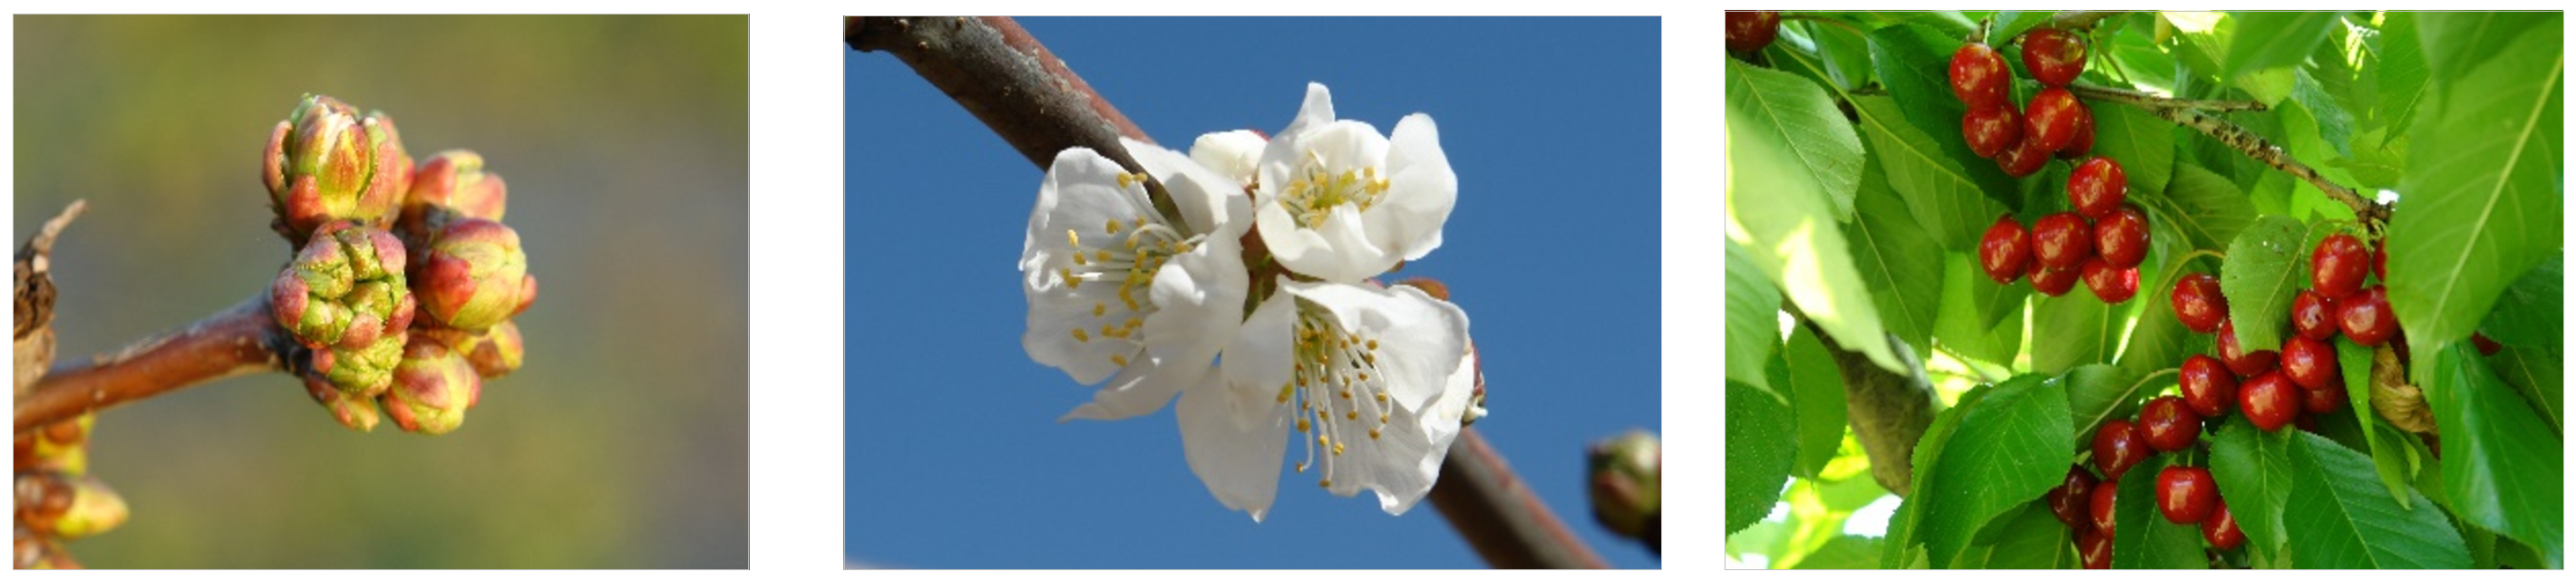
\includegraphics[width=0.9\textwidth,height=\textheight]{pictures/pheno_stages.png}
\caption{Phenological stages of cherry}
\end{figure}

\hypertarget{climate-change-and-impact-projection}{%
\chapter{Climate change and impact projection}\label{climate-change-and-impact-projection}}

Before we get started with \texttt{chillR}, I want to give you an overview of climate change, because much of the work that follows will be focused on forecasting how phenology-related metrics will be impacted by global warming.

\hypertarget{the-drivers-of-climate-change}{%
\section{The drivers of climate change}\label{the-drivers-of-climate-change}}

To fully appreciate what's currently happening to our planet, we need some basic understanding of the drivers of climate change. This also helps prepare us for misleading claims that the sun, urban heat islands or similar peripheral factors are responsible for the alarming global warming we're currently experiencing - or that this warming can be explained by the natural variation of our climate. Spoiler alert: it's totally uncontroversial by now that anthropogenic emissions of greenhouse gases are warming our planet, and the only way to stop this from happening is a drastic reduction of man-made emissions.

\href{https://uni-bonn.sciebo.de/s/b4iTBE82S1CVNx1}{Here are the slides that belong to this video.}

\hypertarget{what-weve-already-seen}{%
\section{What we've already seen}\label{what-weve-already-seen}}

This video presents climatic changes that we've already experienced, or which we have very robust evidence for. Spoiler alert: the planet has been warming dramatically for several decades already, almost everywhere.

\href{https://uni-bonn.sciebo.de/s/5kLiGT77nZyM21w}{Here are the slides that belong to this video.}

\hypertarget{future-scenarios}{%
\section{Future scenarios}\label{future-scenarios}}

When it comes to climate change, the worst is yet to come. This is because the rate of greenhouse gas emissions over the past few decades has been much greater than in the past, and it doesn't look like these emissions will stop very soon. In consequence, the man-made `forcing' effect on our climate has never been greater than now, which makes it likely that future changes will occur even more rapidly than what we've seen so far. This video introduces the methods that climate scientists use to gain a glimpse of the future. It also introduces climate scenarios produced by climate scientists, which can then be used by researchers from other disciplines to project climate change impacts on ecological or agricultural systems.

\href{https://uni-bonn.sciebo.de/s/69LVoQMPWXPFv5I}{Here are the slides that belong to this video.}

\hypertarget{impact-projection-approaches}{%
\section{Impact projection approaches}\label{impact-projection-approaches}}

Having good climate scenarios is important, but it only takes us part of the way towards reliable assessments of climate change impacts. A possibly greater challenge is the translation of climate scenarios into biological consequences. For this, we need impact models, or some other way to derive impacts from climate. This video provides an introduction to climate impact projection methods.

\href{https://uni-bonn.sciebo.de/s/IC87QhJb8hqnDhP}{Here are the slides that belong to this video.}

\hypertarget{exercises_climate_change}{%
\section*{\texorpdfstring{\texttt{Exercises} on climate change}{Exercises on climate change}}\label{exercises_climate_change}}
\addcontentsline{toc}{section}{\texttt{Exercises} on climate change}

Please document all results of the following assignents in your \texttt{learning\ logbook}.

\begin{enumerate}
\def\labelenumi{\arabic{enumi})}
\item
  List the main drivers of climate change at the decade to century scale, and briefly explain the mechanism through which the currently most important driver affects our climate.
\item
  Explain briefly what is special about temperature dynamics of the recent decades, and why we have good reasons to be concerned.
\item
  What does the abbreviation `RCP' stand for, how are RCPs defined, and what is their role in projecting future climates?
\item
  Briefly describe the 4 climate impact projection methods described in the fourth video.
\end{enumerate}

\hypertarget{winter-chill-projections}{%
\chapter{Winter chill projections}\label{winter-chill-projections}}

\hypertarget{goals_analysis_examples}{%
\section*{Learning goals for this lesson}\label{goals_analysis_examples}}
\addcontentsline{toc}{section}{Learning goals for this lesson}

\begin{itemize}
\tightlist
\item
  Be aware of past studies that have projected climate change impacts on winter chill
\item
  Get a rough idea of how such studies are done
\item
  Get curious about how to do such studies
\end{itemize}

\hypertarget{winter-chill-projections-1}{%
\section{Winter chill projections}\label{winter-chill-projections-1}}

This lesson will give you an overview of how winter chill can be modeled. More precisely, it will be a little tour of the studies I've done on this in the past. I'll lead you through these studies to help you understand how the methodological pieces of the puzzle fit together. If everything goes according to plan, you should be able to do most of the analyses that are behind these papers after completing this class.

\hypertarget{winter-chill-in-oman}{%
\subsection{Winter chill in Oman}\label{winter-chill-in-oman}}

As a student at the \href{https://www.uni-kassel.de/fb11agrar/fachgebiete-einrichtungen/opats/startseite.html}{University of Kassel}, I had the chance to participate in research projects focusing on mountain oases in the Sultanate of Oman. I also worked on these systems for my PhD, where I first started to get interested in winter chill. This wasn't the original study plan. We were going to calculate nutrient budgets for the oases, and this required measuring the yields of the various fruit trees there. Here's an impression of the oasis orchards:

\begin{figure}
\centering
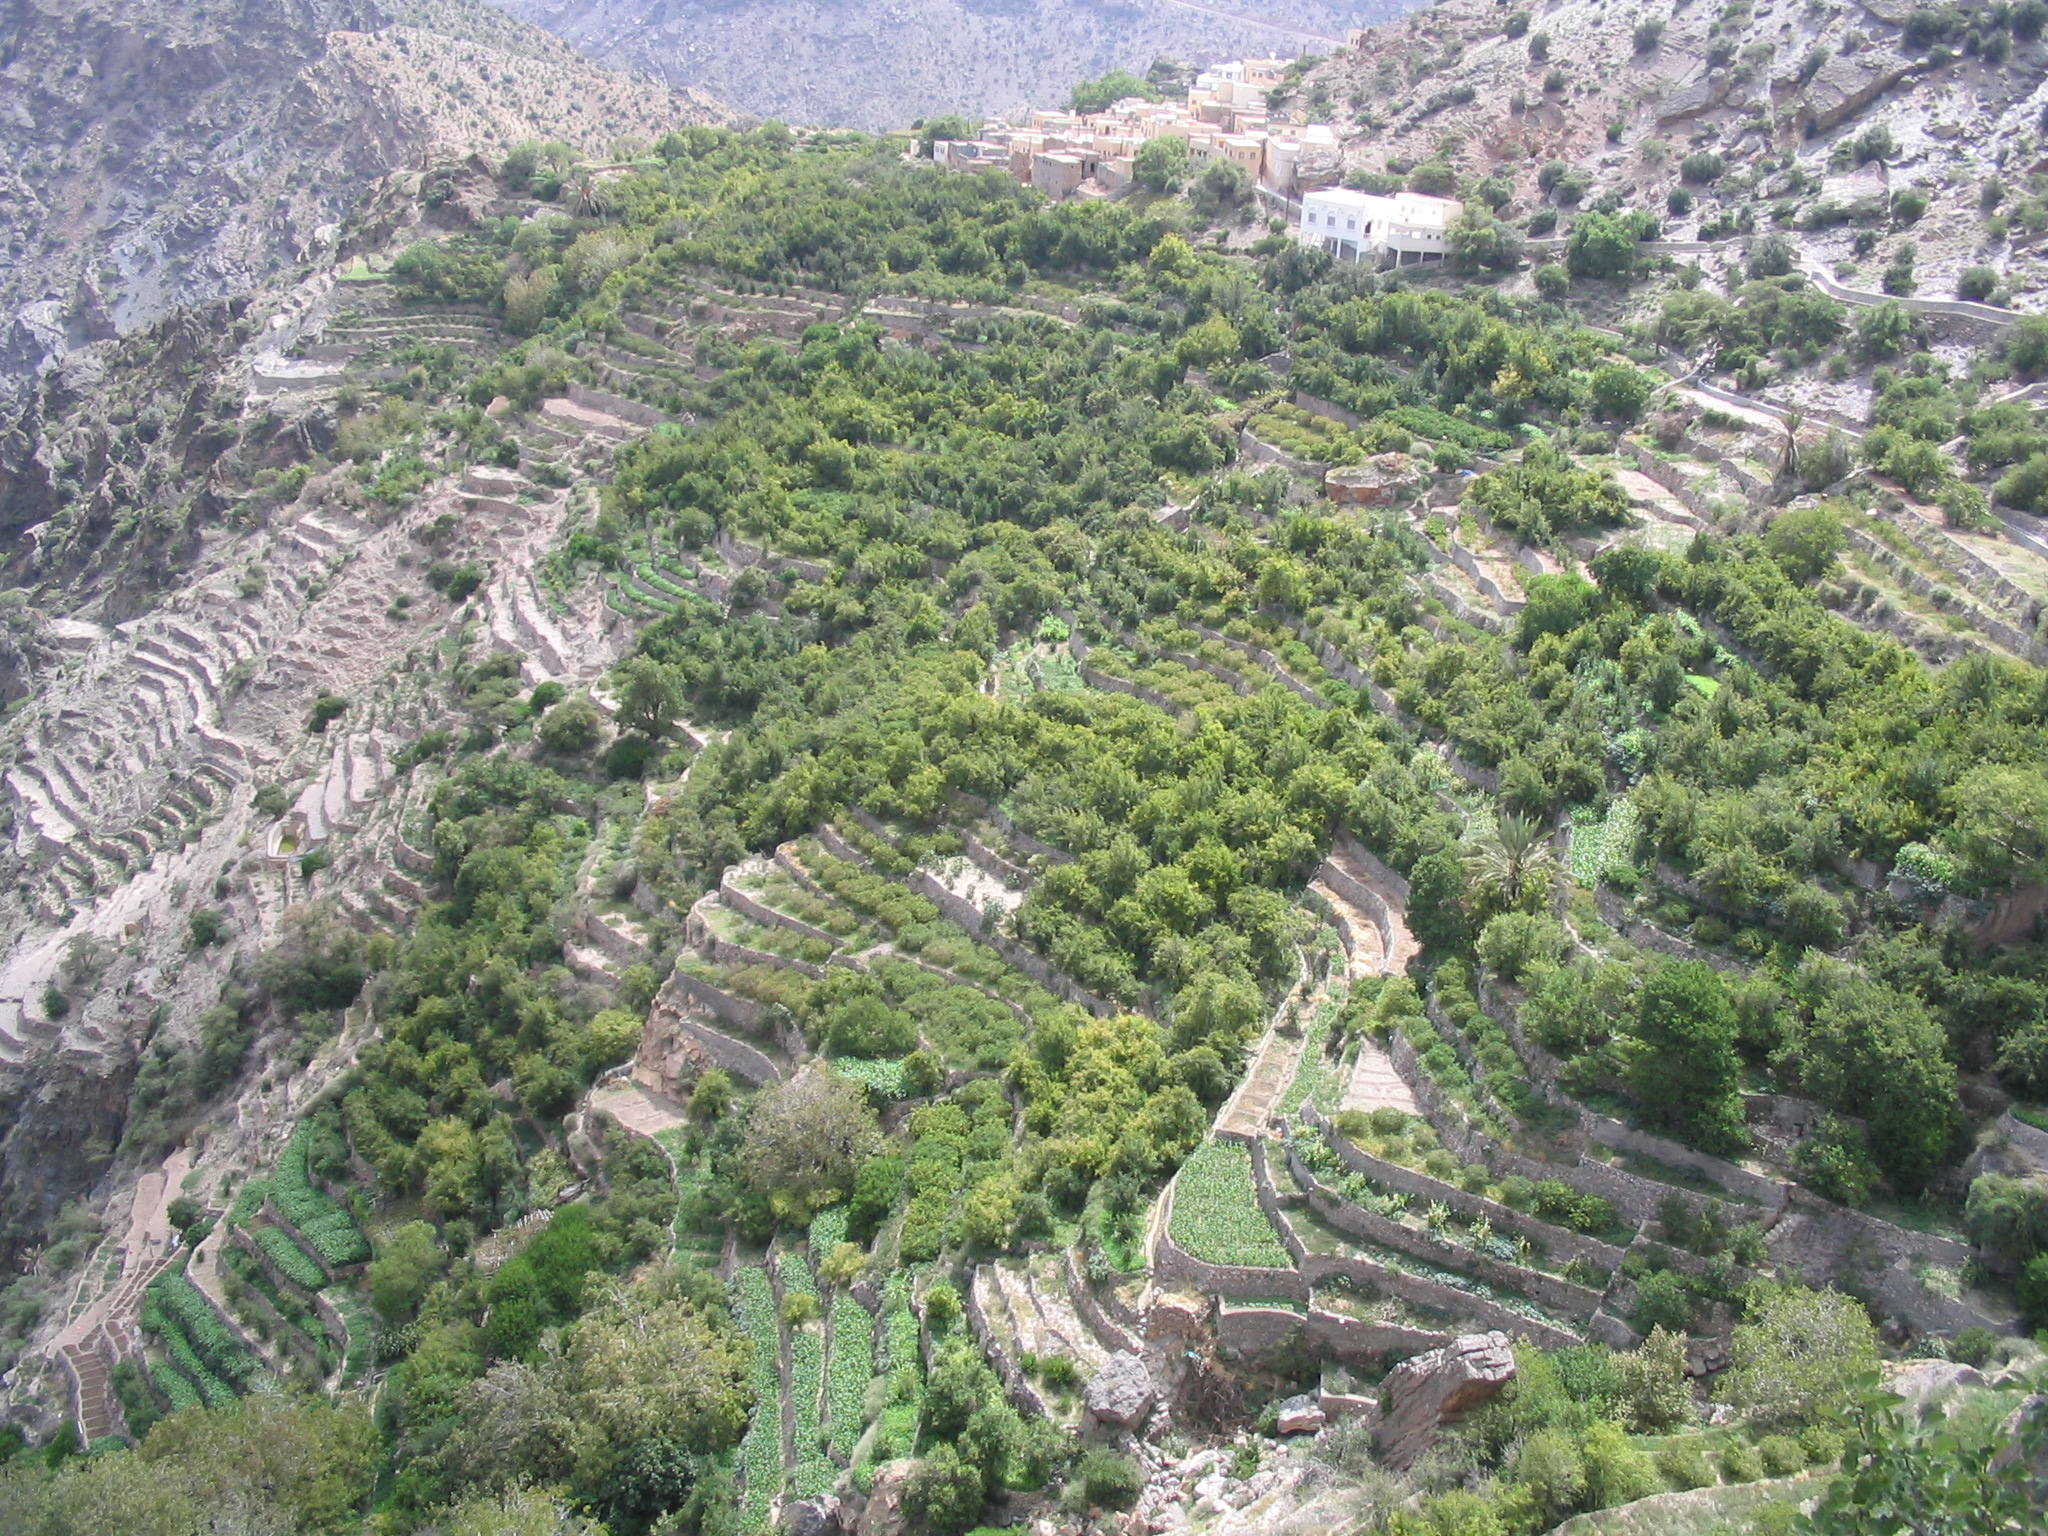
\includegraphics[width=0.9\textwidth,height=\textheight]{pictures/IMG_8538.JPG}
\caption{The `Hanging Gardens' of Ash Sharayjah, one of the oases of Al Jabal Al Akhdar}
\end{figure}

This is where you can find these beautiful villages:

\begin{figure}
\centering
\includegraphics{Book_files/figure-latex/unnamed-chunk-4-1.pdf}
\caption{\label{fig:unnamed-chunk-4}Location of the oases of Al Jabal Al Akhdar in the Sultanate of Oman}
\end{figure}

Unfortunately, many of the trees in the oasis system we worked in produced no fruits in the years we were there. One of my colleagues, \href{https://scholar.google.de/citations?user=2UgqSrEAAAAJ\&hl=en\&oi=ao}{Jens Gebauer} (now \href{https://www.hochschule-rhein-waal.de/en/faculties/life-sciences/organisation/professors/prof-dr-habil-jens-gebauer}{Professor of Horticultural Sciences at Rhine-Waal University of Applied Sciences}) suggested that this could have something to do with lack of chilling. This made sense, because most of the trees in these high-altitude oases were not the typical species of the Arabian Peninsula, but temperate trees, such as the pomegranates (\href{https://en.wikipedia.org/wiki/Pomegranate}{\emph{Punica granatum}}), walnuts (\href{https://en.wikipedia.org/wiki/Walnut}{\emph{Juglans regia}}) or apricots (\href{https://en.wikipedia.org/wiki/Apricot}{\emph{Prunus armeniaca}}), as you can see here:

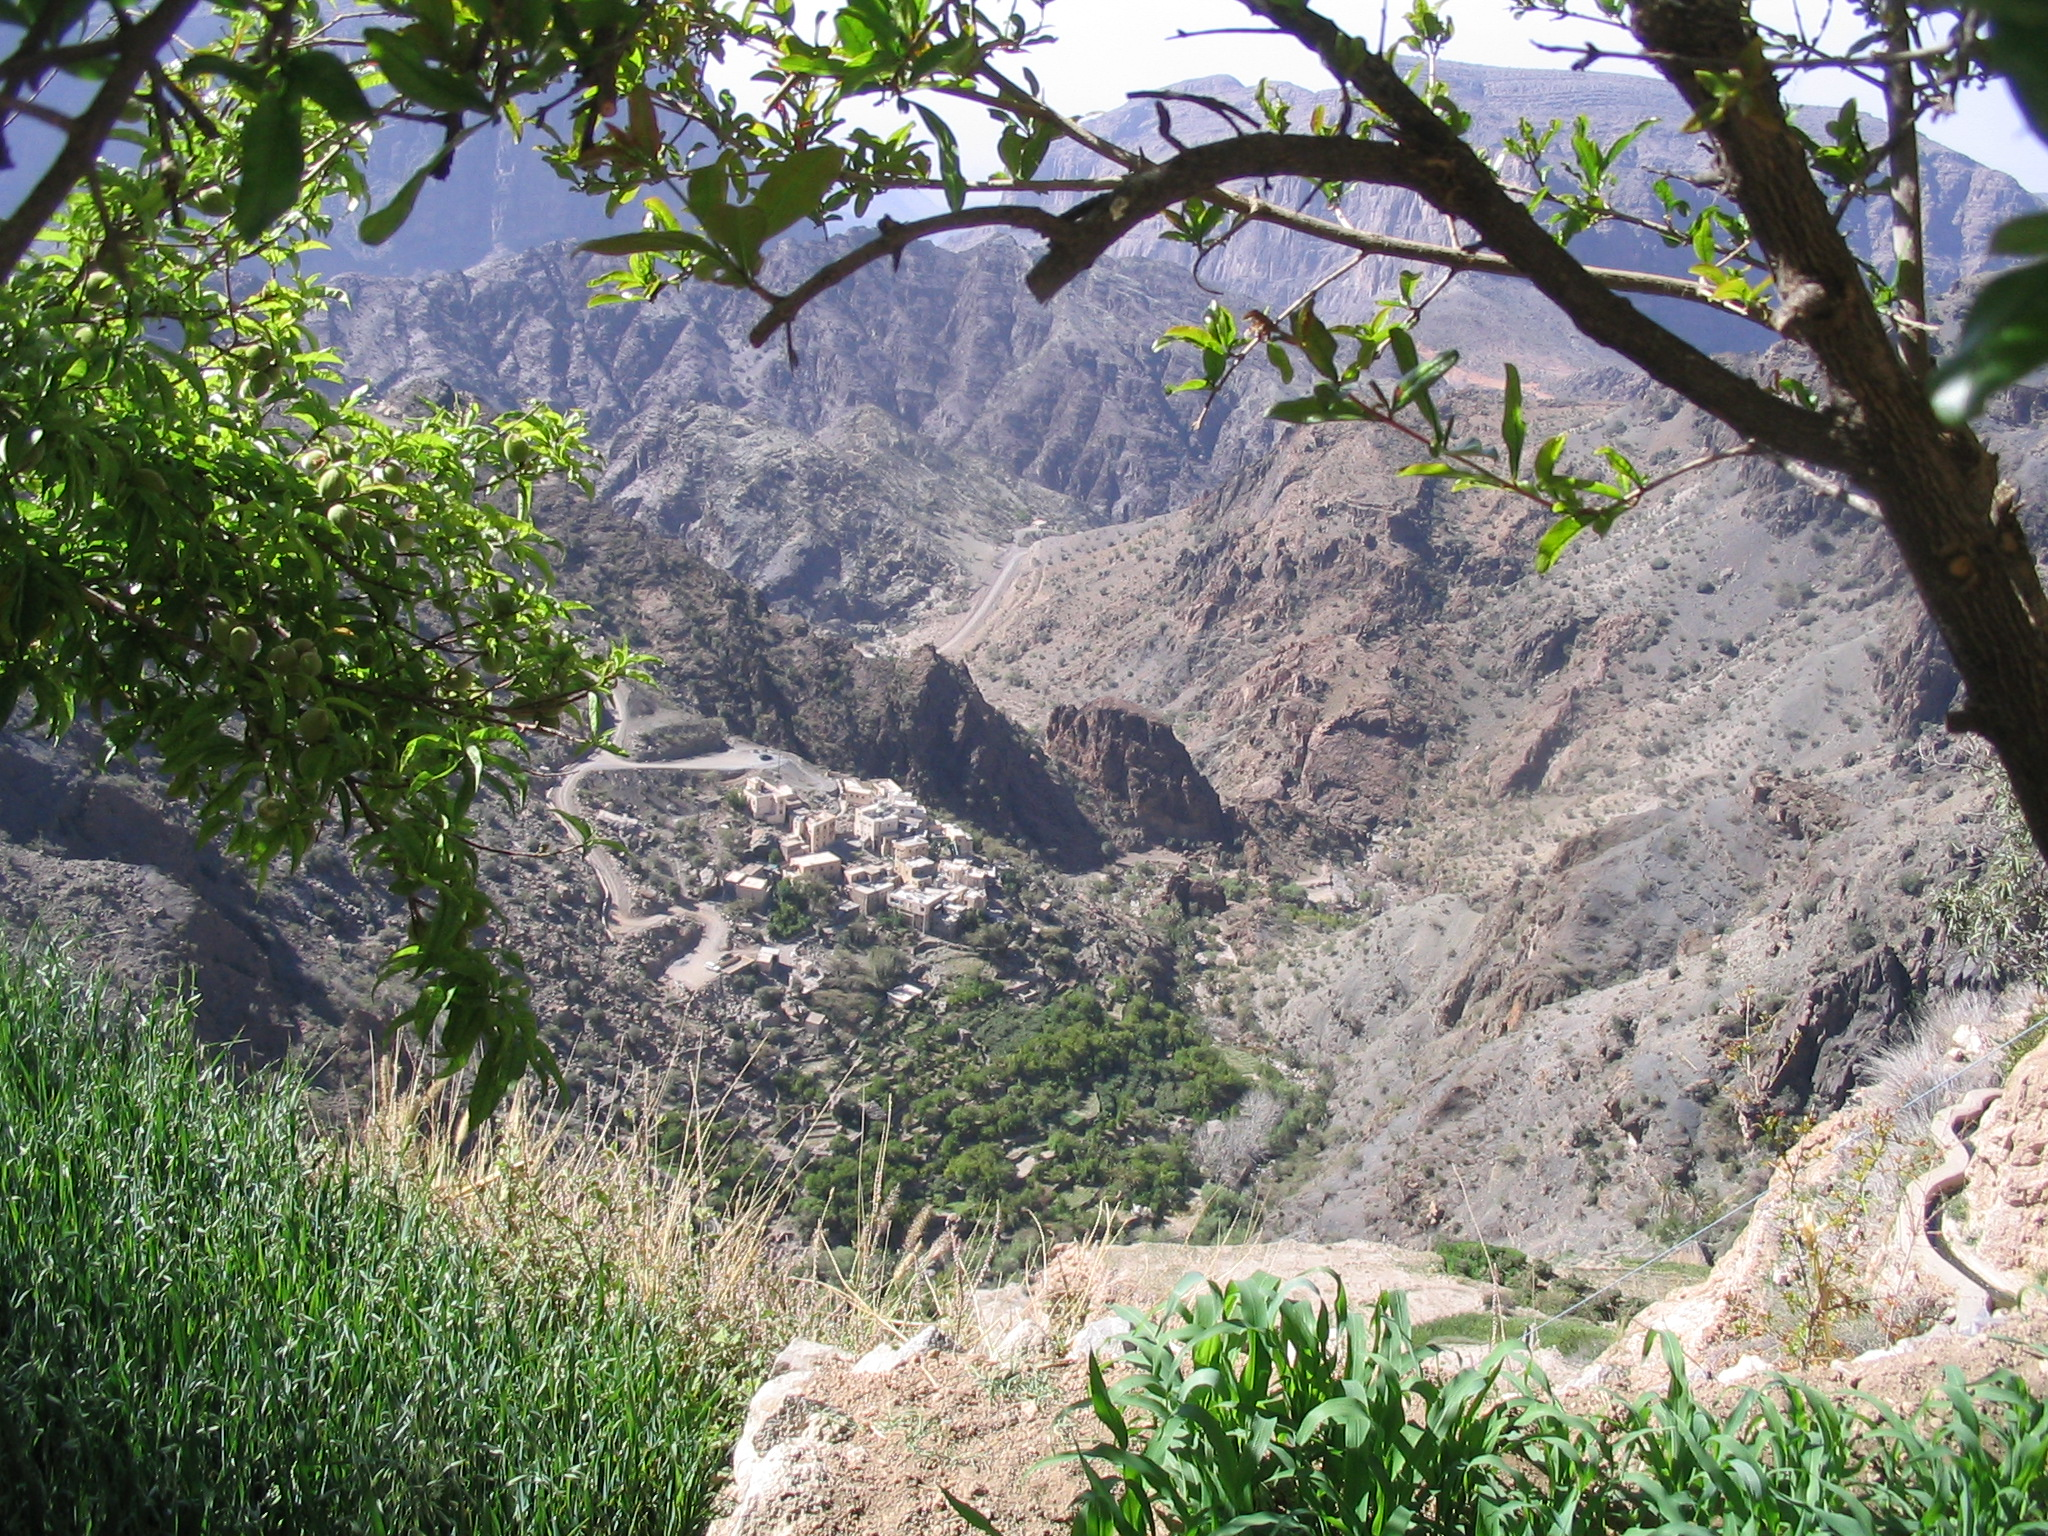
\includegraphics[width=0.33\textwidth,height=\textheight]{pictures/IMG_7190.JPG} 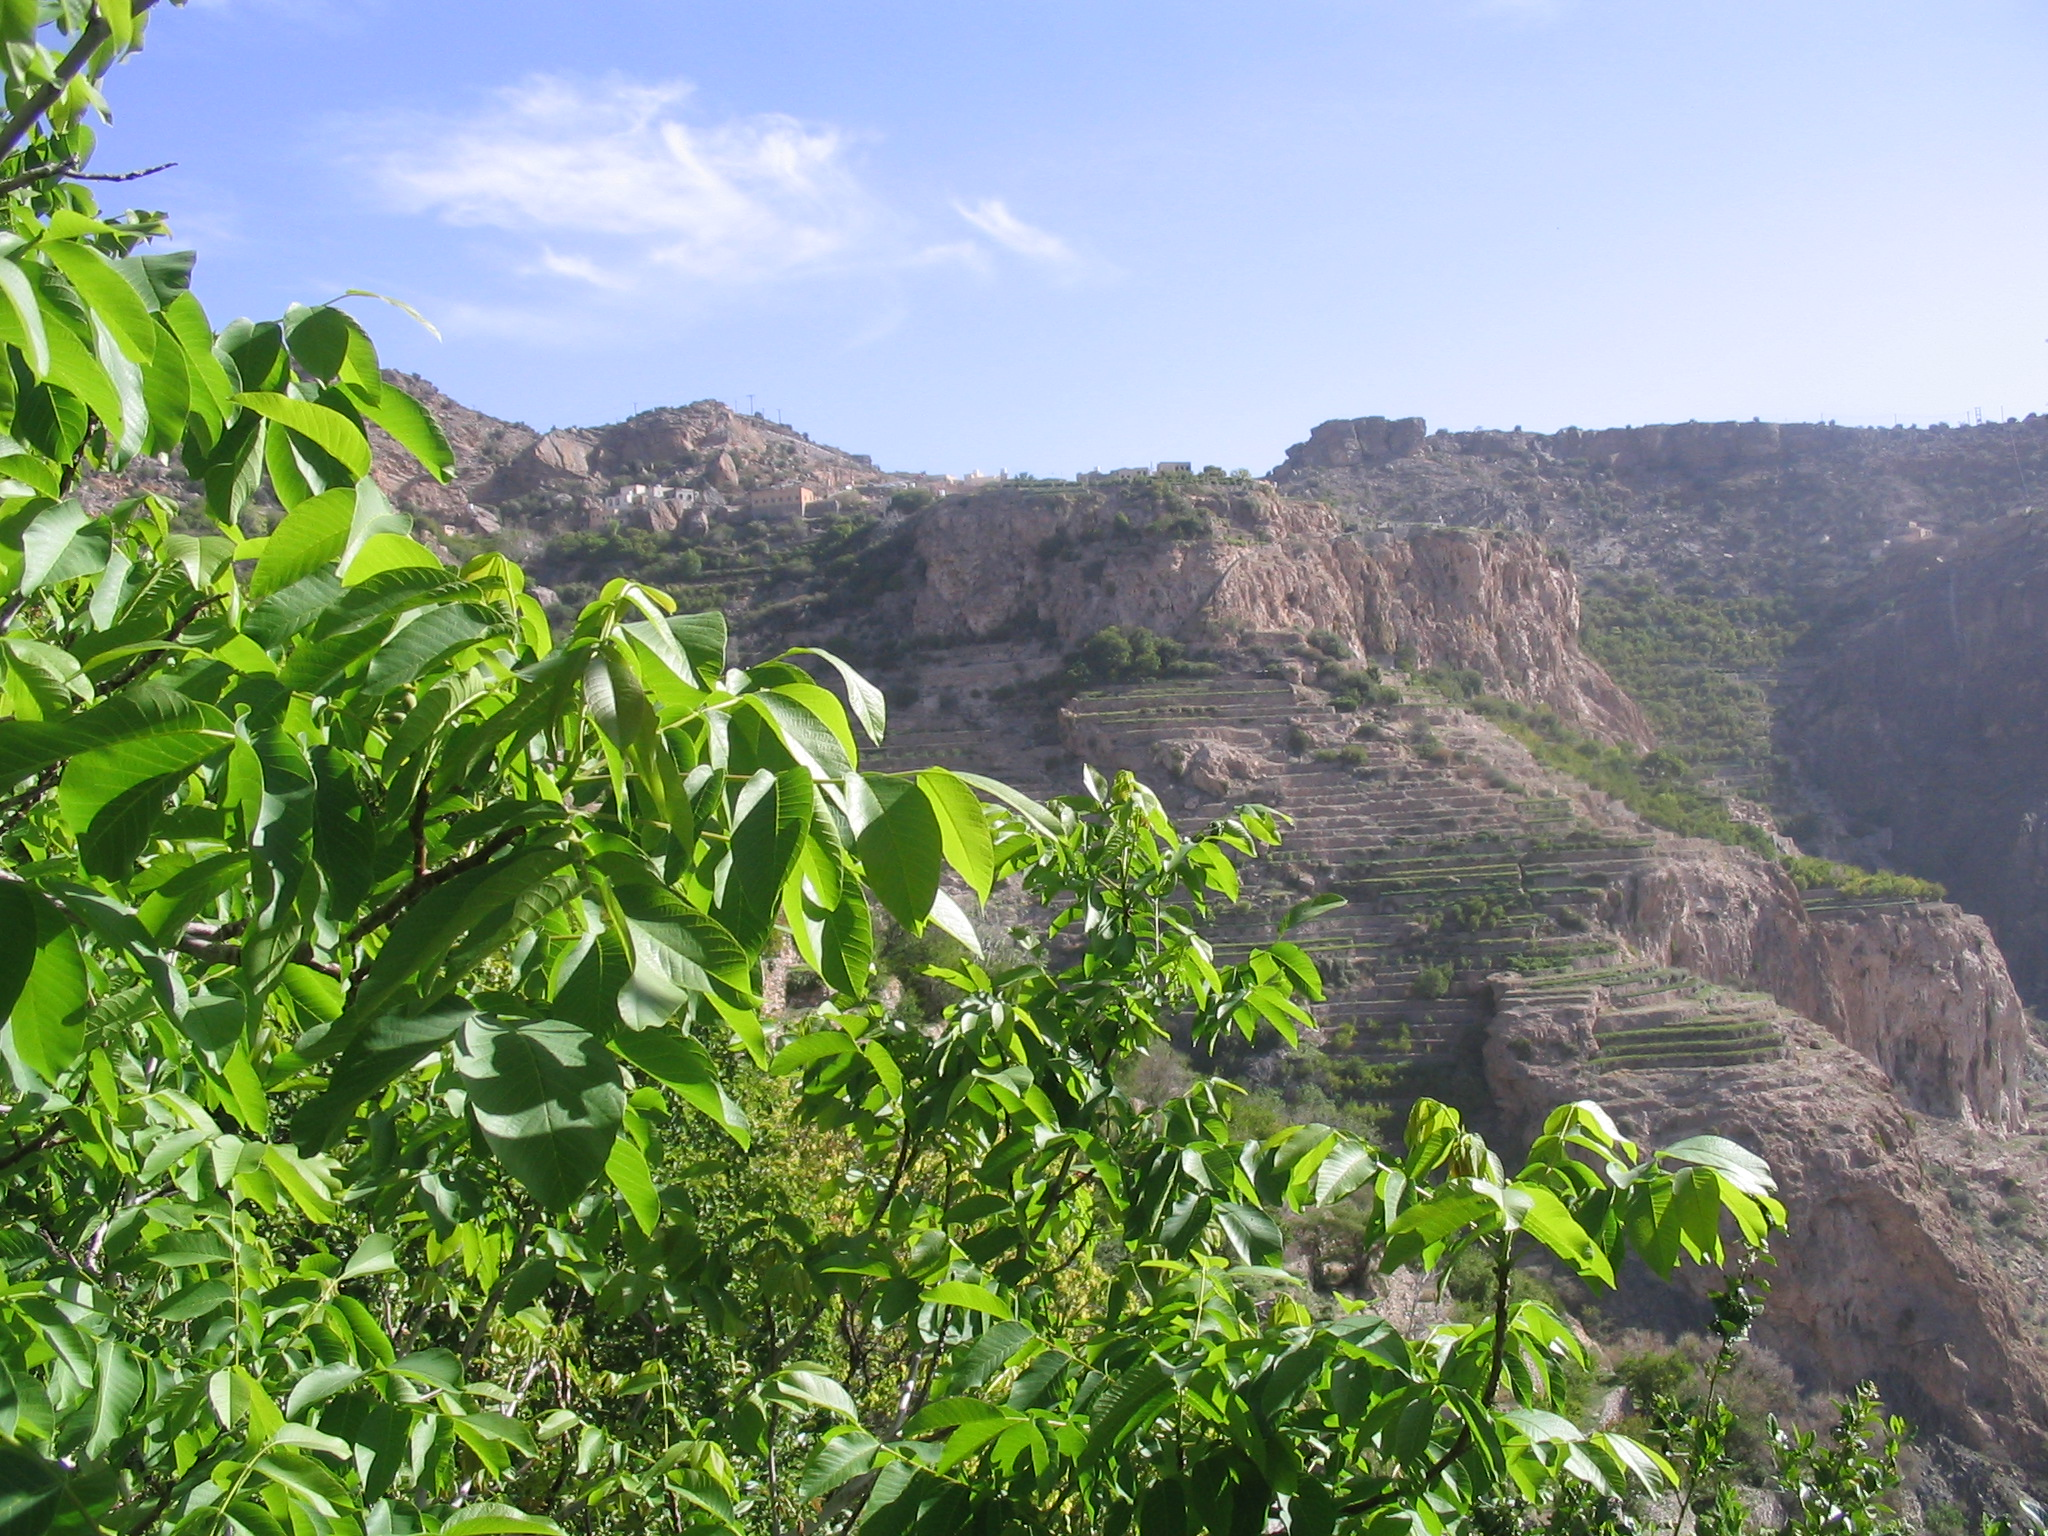
\includegraphics[width=0.33\textwidth,height=\textheight]{pictures/IMG_7332.JPG} 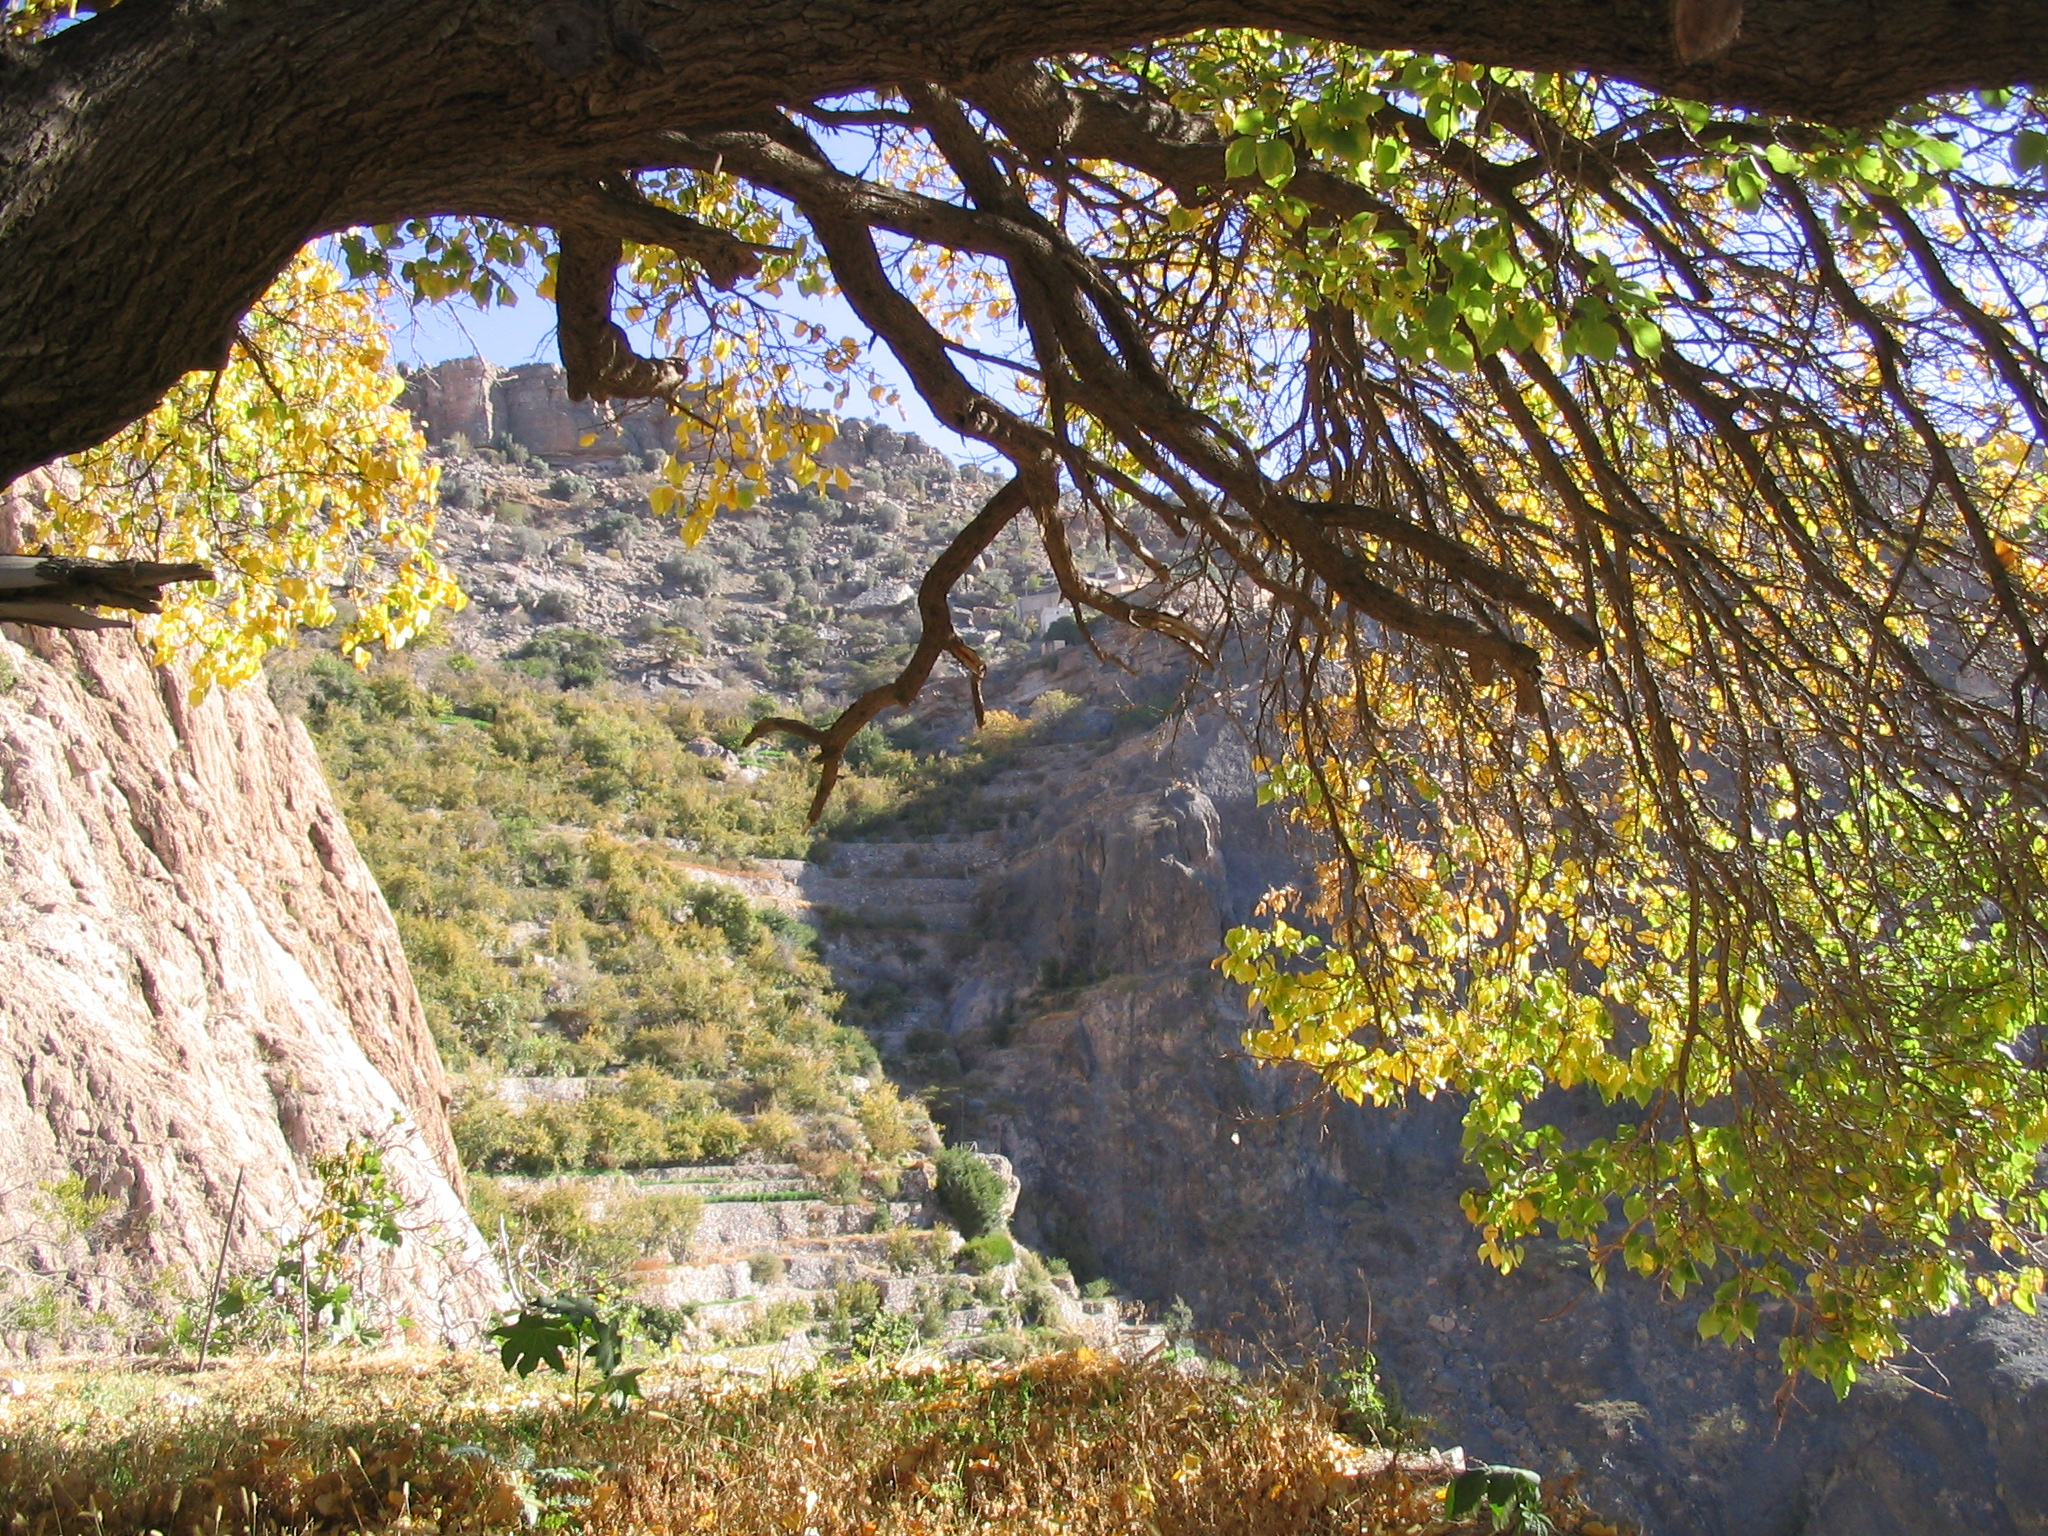
\includegraphics[width=0.33\textwidth,height=\textheight]{pictures/IMG_5690.JPG}

So, rather than focusing on the nutrient budgets, I started looking into this.

I quickly came across the Chilling Hours model, which I assumed would be a suitable model to quantify chill. I later realized that this model can't really be trusted, especially in such a warm location (we're at almost 2000 m of elevation here, but it's still pretty warm), but I didn't know that then (many people still don't seem to know this, even today).

We had placed temperature loggers in three oases at different levels of elevation, which allowed studying chill accumulation along an elevation gradient. Here's a map of the study area:

\begin{figure}
\centering
\includegraphics{pictures/Fig_01_gradient_map.jpg}
\caption{Map of oasis systems in Al Jabal Al Akhdar, Oman}
\end{figure}

The temperature loggers were installed in small sensor shelters, such as the one you see in the image below. Note that this is the one in Masayrat ar Ruwajah, the lowest oasis along the gradient. This is why in this picture, we see the heat-loving date palm (\href{https://en.wikipedia.org/wiki/Date_palm}{\emph{Phoenix dactylifera}}), rather than temperate trees.

\begin{figure}
\centering
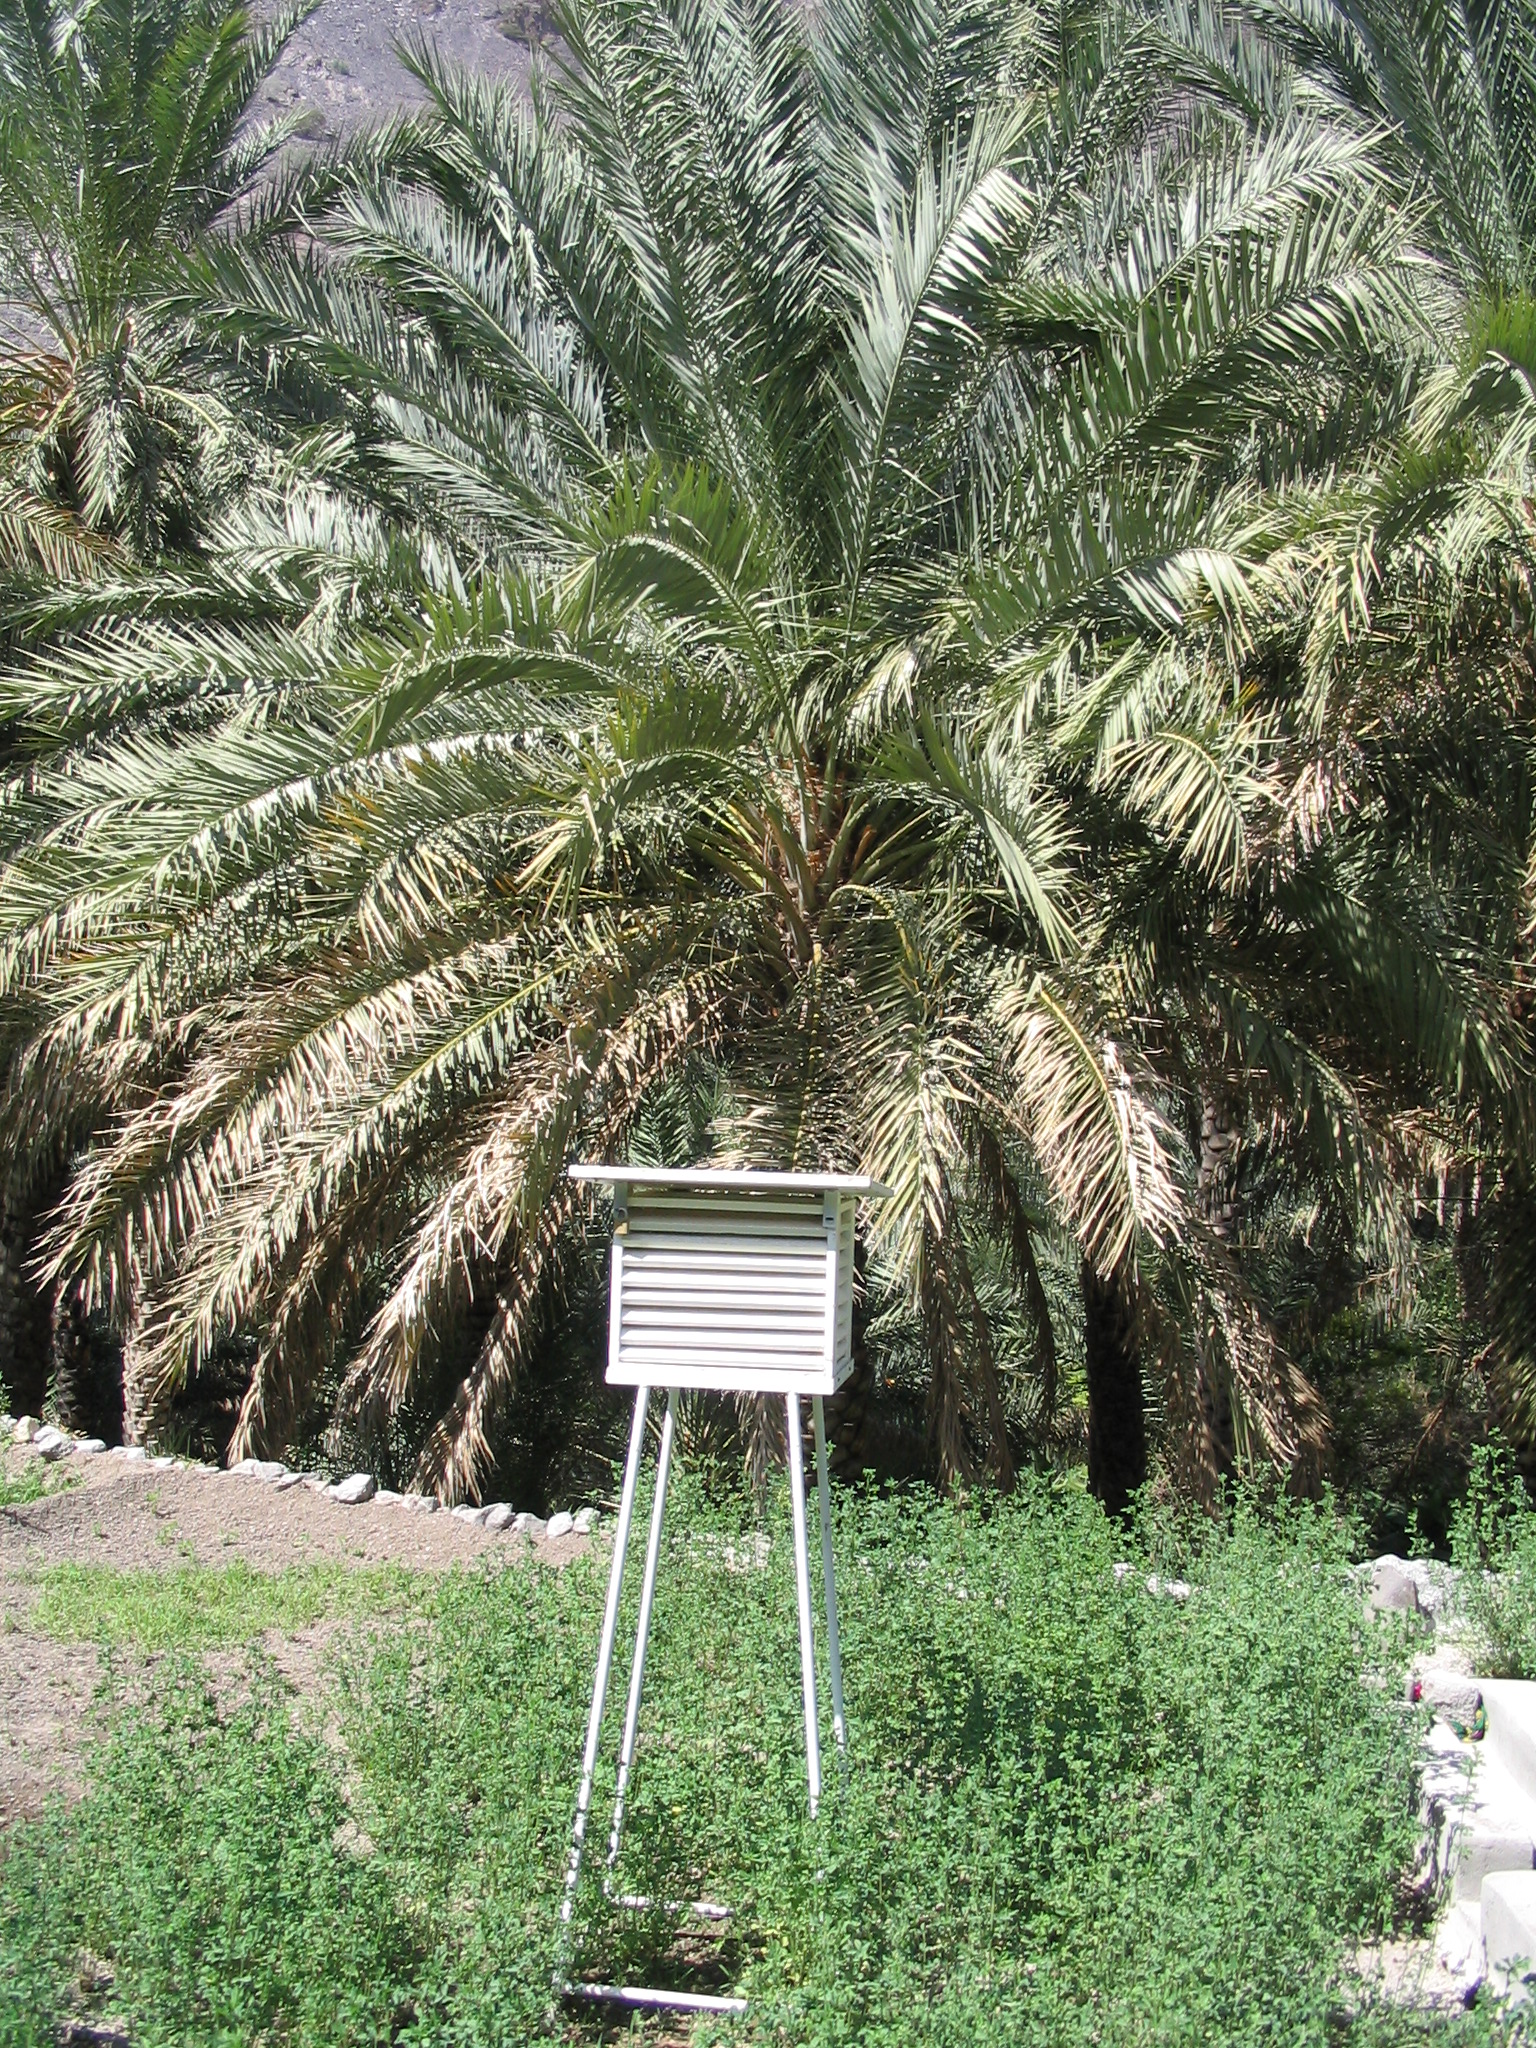
\includegraphics[width=0.5\textwidth,height=\textheight]{pictures/IMG_5298.JPG}
\caption{Temperature logger in Masayrat ar Ruwajah, Al Jabal Al Akhdar, Oman}
\end{figure}

If you want to do a climate change analysis, you can't really just put up a temperature sensor and hope to collect meaningful data in a reasonable period of time. Fortunately for us, an official long-term weather station is located in the vicinity, near the top of the valley. However, this station is roughly 1000 m above the lowest oasis, and it is clear that its readings aren't representative of all locations along the elevation gradient.

Since we had records from the oases, however, we were able to define transfer functions that allowed deriving oasis temperatures from the long-term data. We set these transfer functions up (using PLS regression, which in hindsight wasn't a very good idea) to directly calculate hourly temperatures in the oases from the daily records of the official station at Saiq.

\begin{figure}
\centering
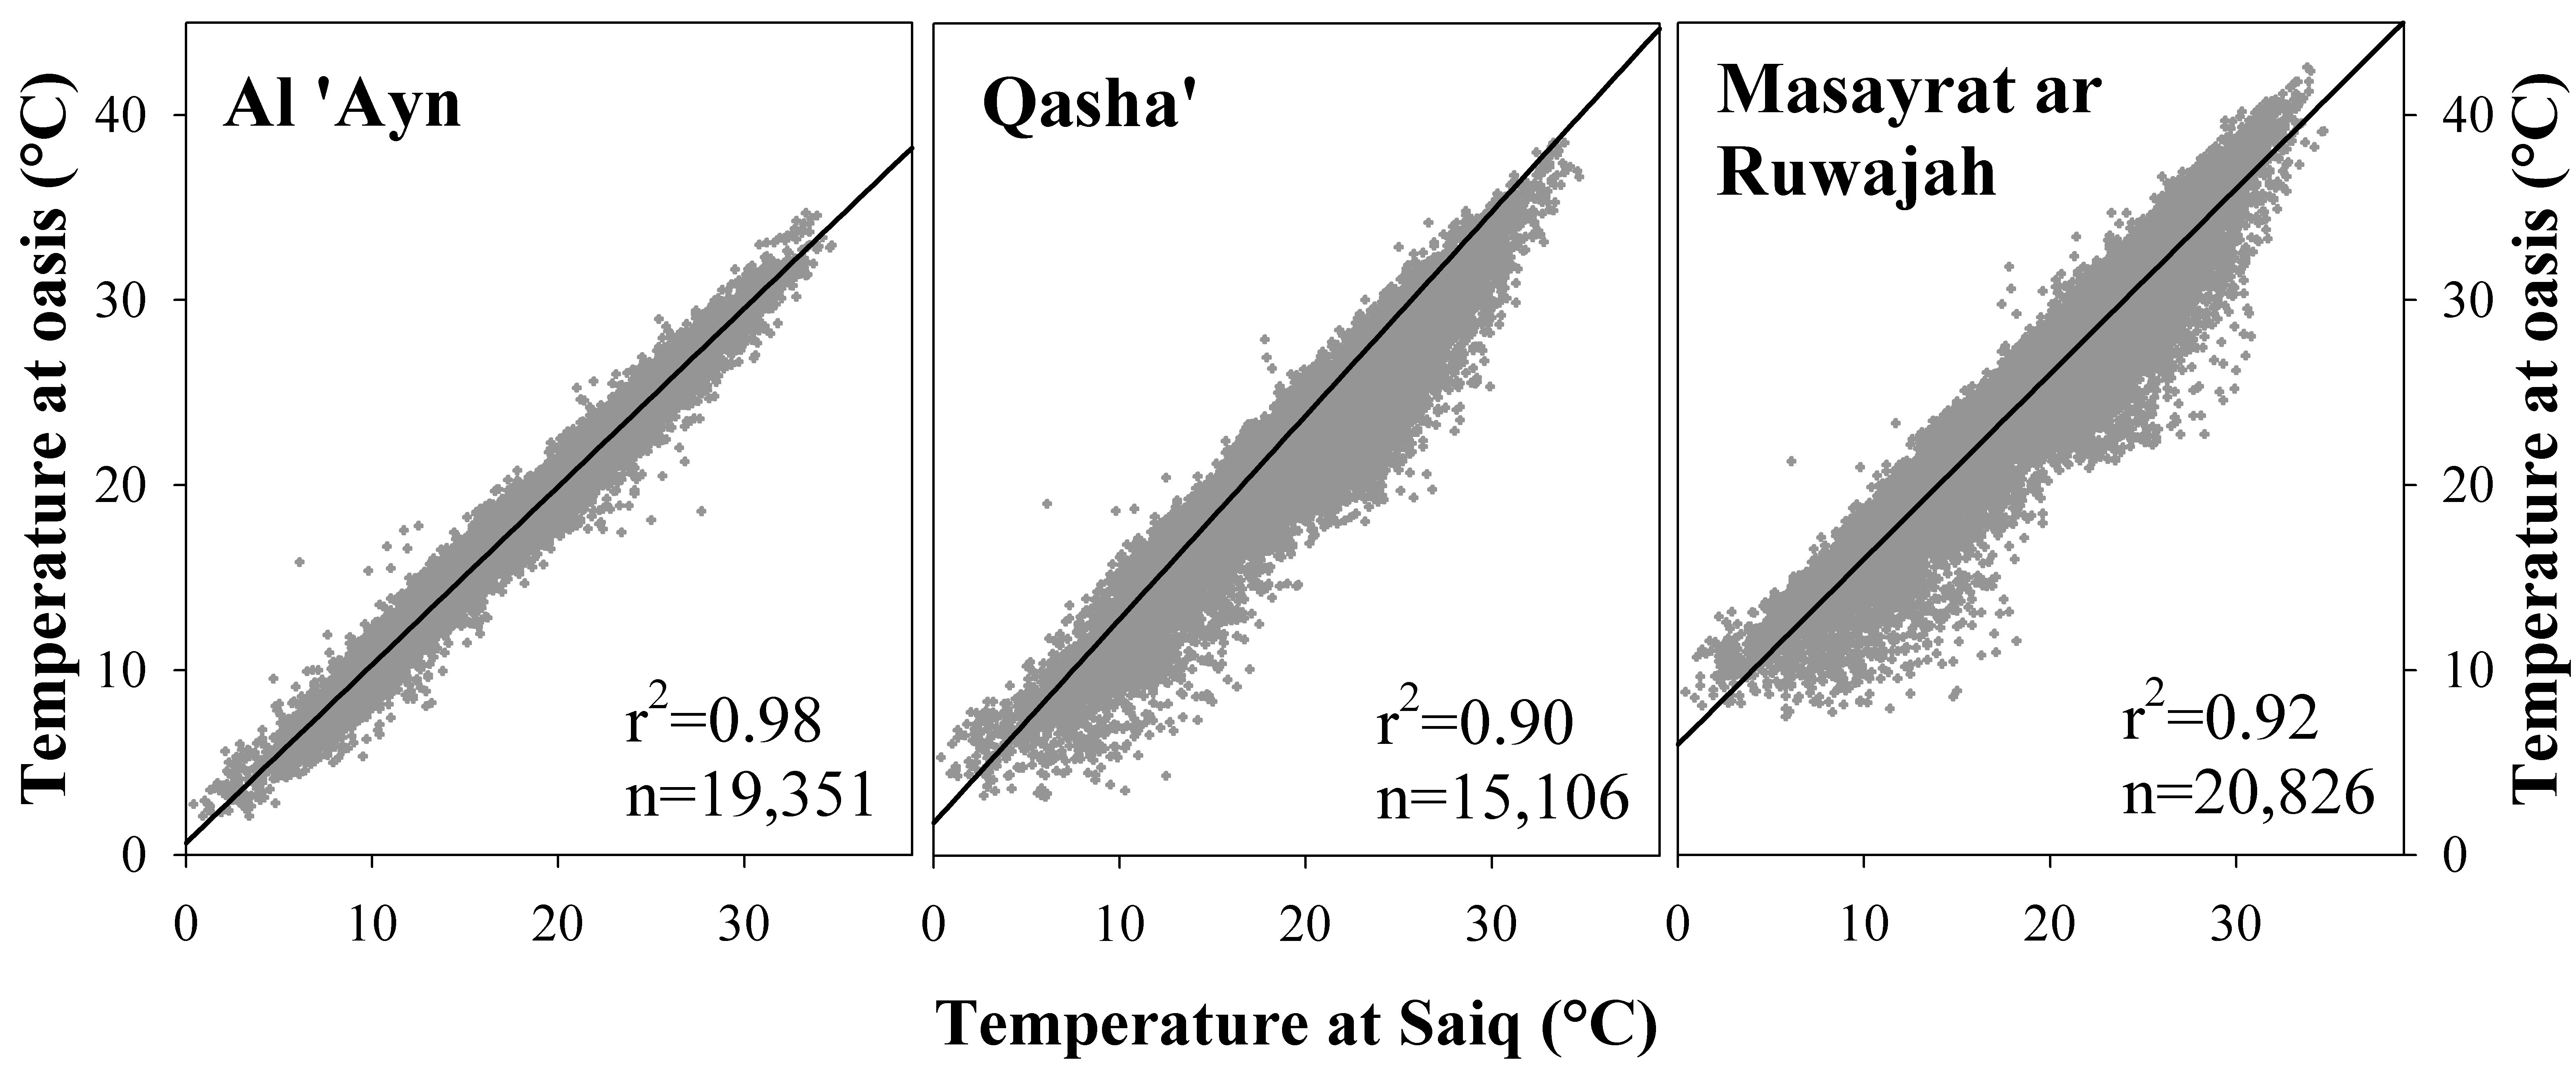
\includegraphics[width=0.9\textwidth,height=\textheight]{pictures/Luedeling_JPG_Figure_02_Hourly_regressions.JPG}
\caption{Regression between temperature at Saiq and temperature in three oases, Al Jabal Al Akhdar, Oman}
\end{figure}

Hourly data were needed to calculate the number of Chilling Hours, so this procedure allowed us to calculate winter chill dynamics over the entire time span covered by the official weather station:

\begin{figure}
\centering
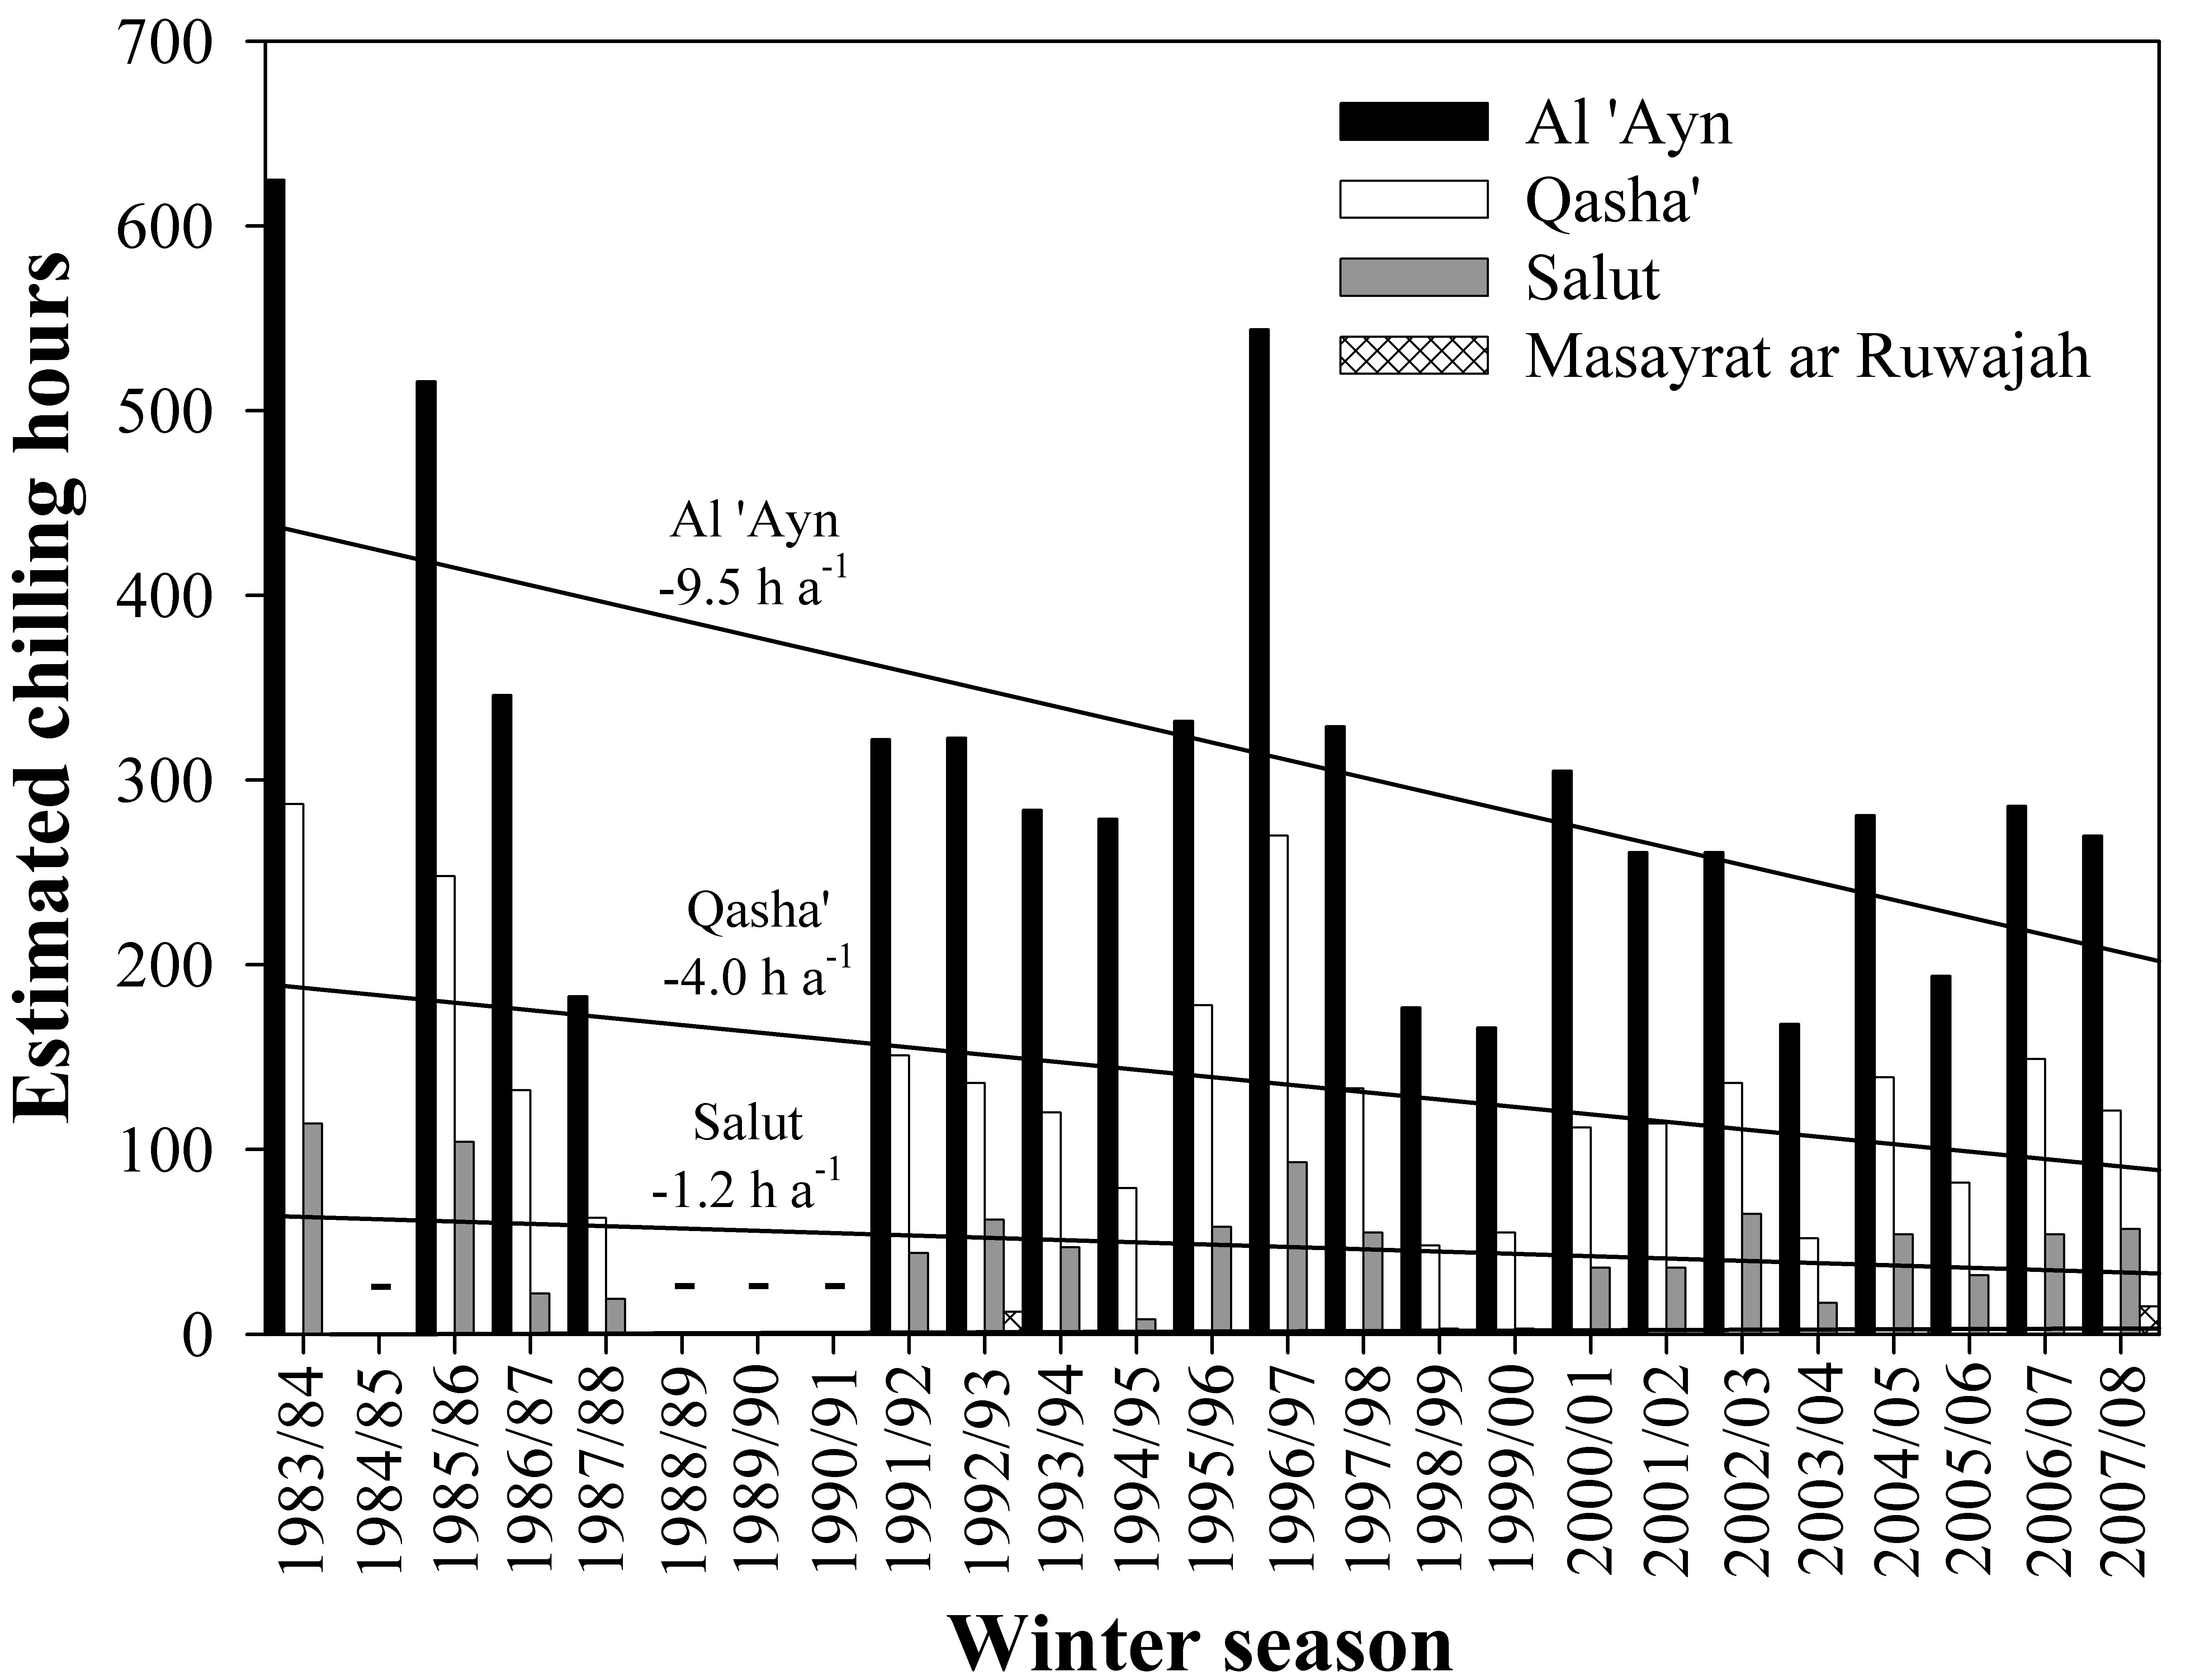
\includegraphics[width=0.9\textwidth,height=\textheight]{pictures/Luedeling_JPG_Figure_09_chilling_hours.JPG}
\caption{Chill dynamics between 1983 and 2007, Al Jabal Al Akhdar, Oman}
\end{figure}

We submitted a manuscript on this analysis to the journal \href{https://www.springer.com/journal/10584?gclid=EAIaIQobChMItKTqpKOF7AIVhZSyCh2taQD4EAAYASAAEgLRIfD_BwE}{Climatic Change}. The reviewers there generally liked the study, but they requested that we add future climate scenarios. This is when I first came across a weather generator. Weather generators are tools that can produce random draws of plausible weather, based on observed weather for a particular location.

So we fed such a weather generator (in this case the \href{https://sites.google.com/view/lars-wg/}{LARS-WG weather generator} maintained by \href{https://scholar.google.com/citations?user=FDj5OJMAAAAJ\&hl=en}{Mikhail Semenov}) with the data we had for the highest-elevation oasis and told it to generate plausible weather for a number of years for us. We also requested the generator to produce comparable records for possible future scenarios, where temperatures were 1 and 2°C higher than in the historic period. We used our transfer functions on these datasets, and got the following results:

\begin{figure}
\centering
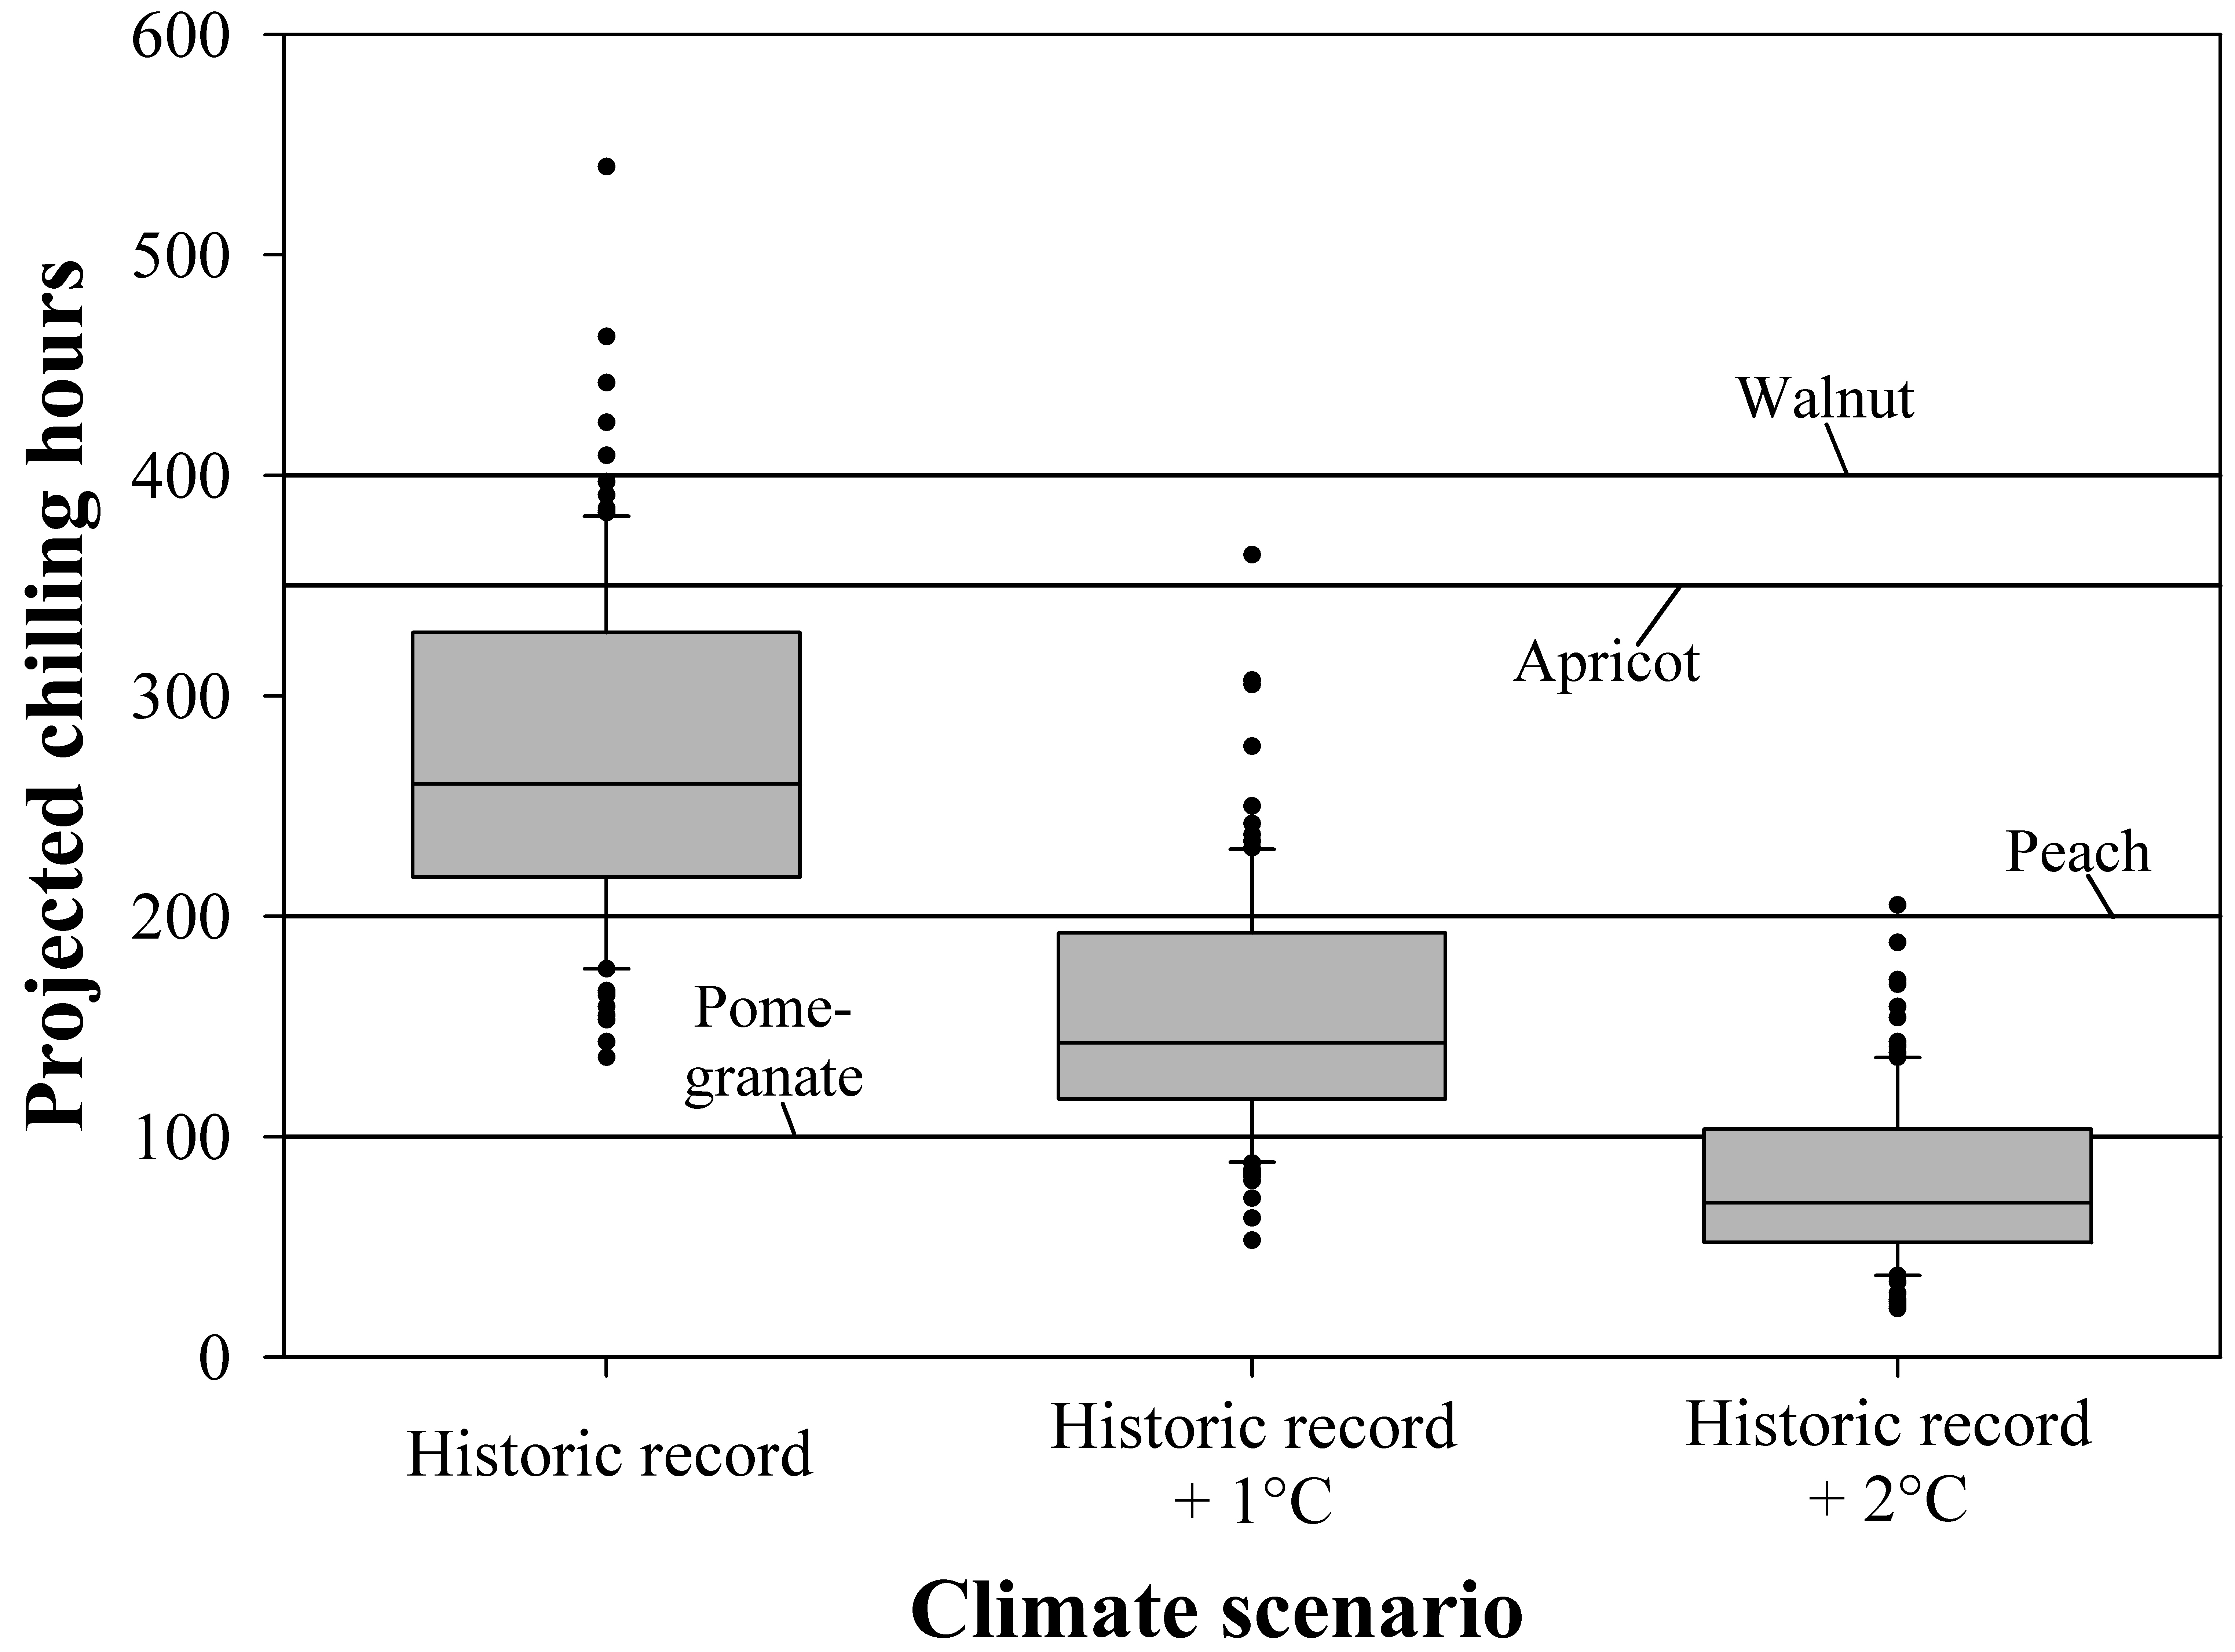
\includegraphics[width=0.9\textwidth,height=\textheight]{pictures/Luedeling_JPG_Figure_10_Future_chilling.JPG}
\caption{Chill prospects for 1°C and 2°C warming scenarios in Al Jabal Al Akhdar, Oman}
\end{figure}

This study, which was ultimately accepted by Climatic Change \href{https://link.springer.com/article/10.1007/s10584-009-9581-7}{(Luedeling, Gebauer, and Buerkert \protect\hyperlink{ref-luedeling_climate_2009}{2009})}, was the beginning of my chill modeling career. Turns our there was still a lot to learn\ldots{}

\hypertarget{chill-model-sensitivity}{%
\subsection{Chill model sensitivity}\label{chill-model-sensitivity}}

After finishing my PhD in Kassel, I moved to the \href{https://www.ucdavis.edu/}{University of California at Davis} to work as a Postdoctoral Scholar (I had already done an \href{https://iad.ucdavis.edu/}{MSc in International Agricultural Development} there, and I wrote a grant proposal with \href{http://agis.ucdavis.edu/people/minghua_zhang/index.html}{Prof.~Minghua Zhang}, whose lab I had been working in then). The new project was on projecting climate change impacts on winter chill in the Central Valley, one of the world's most productive regions for temperate fruit trees.

The first thing I noticed is that the choice of chill model matters - a lot! I had noticed that there are different models to quantify winter chill, but - like many modelers - I decided to go with the one that seemed easiest to handle. This may have been unavoidable at the time, because I had zero programming skills, but this is really not how we should choose models! We'll see a bit more evidence of what errors can result from this later.

After I arrived in California, one of the first things I did was disappear into the library for quite some time to read everything I could find on winter chill. What I found made it pretty clear that model choice was worth looking into. So I used the methodological knowledge I had gained in Oman, created a bunch of temperature scenarios for multiple locations and calculated how chill accumulation was likely to change in the future, according to multiple chill models.

I looked at what changes the various models predicted for the same locations and the same future scenarios. Here are the locations I looked at:

\begin{figure}
\centering
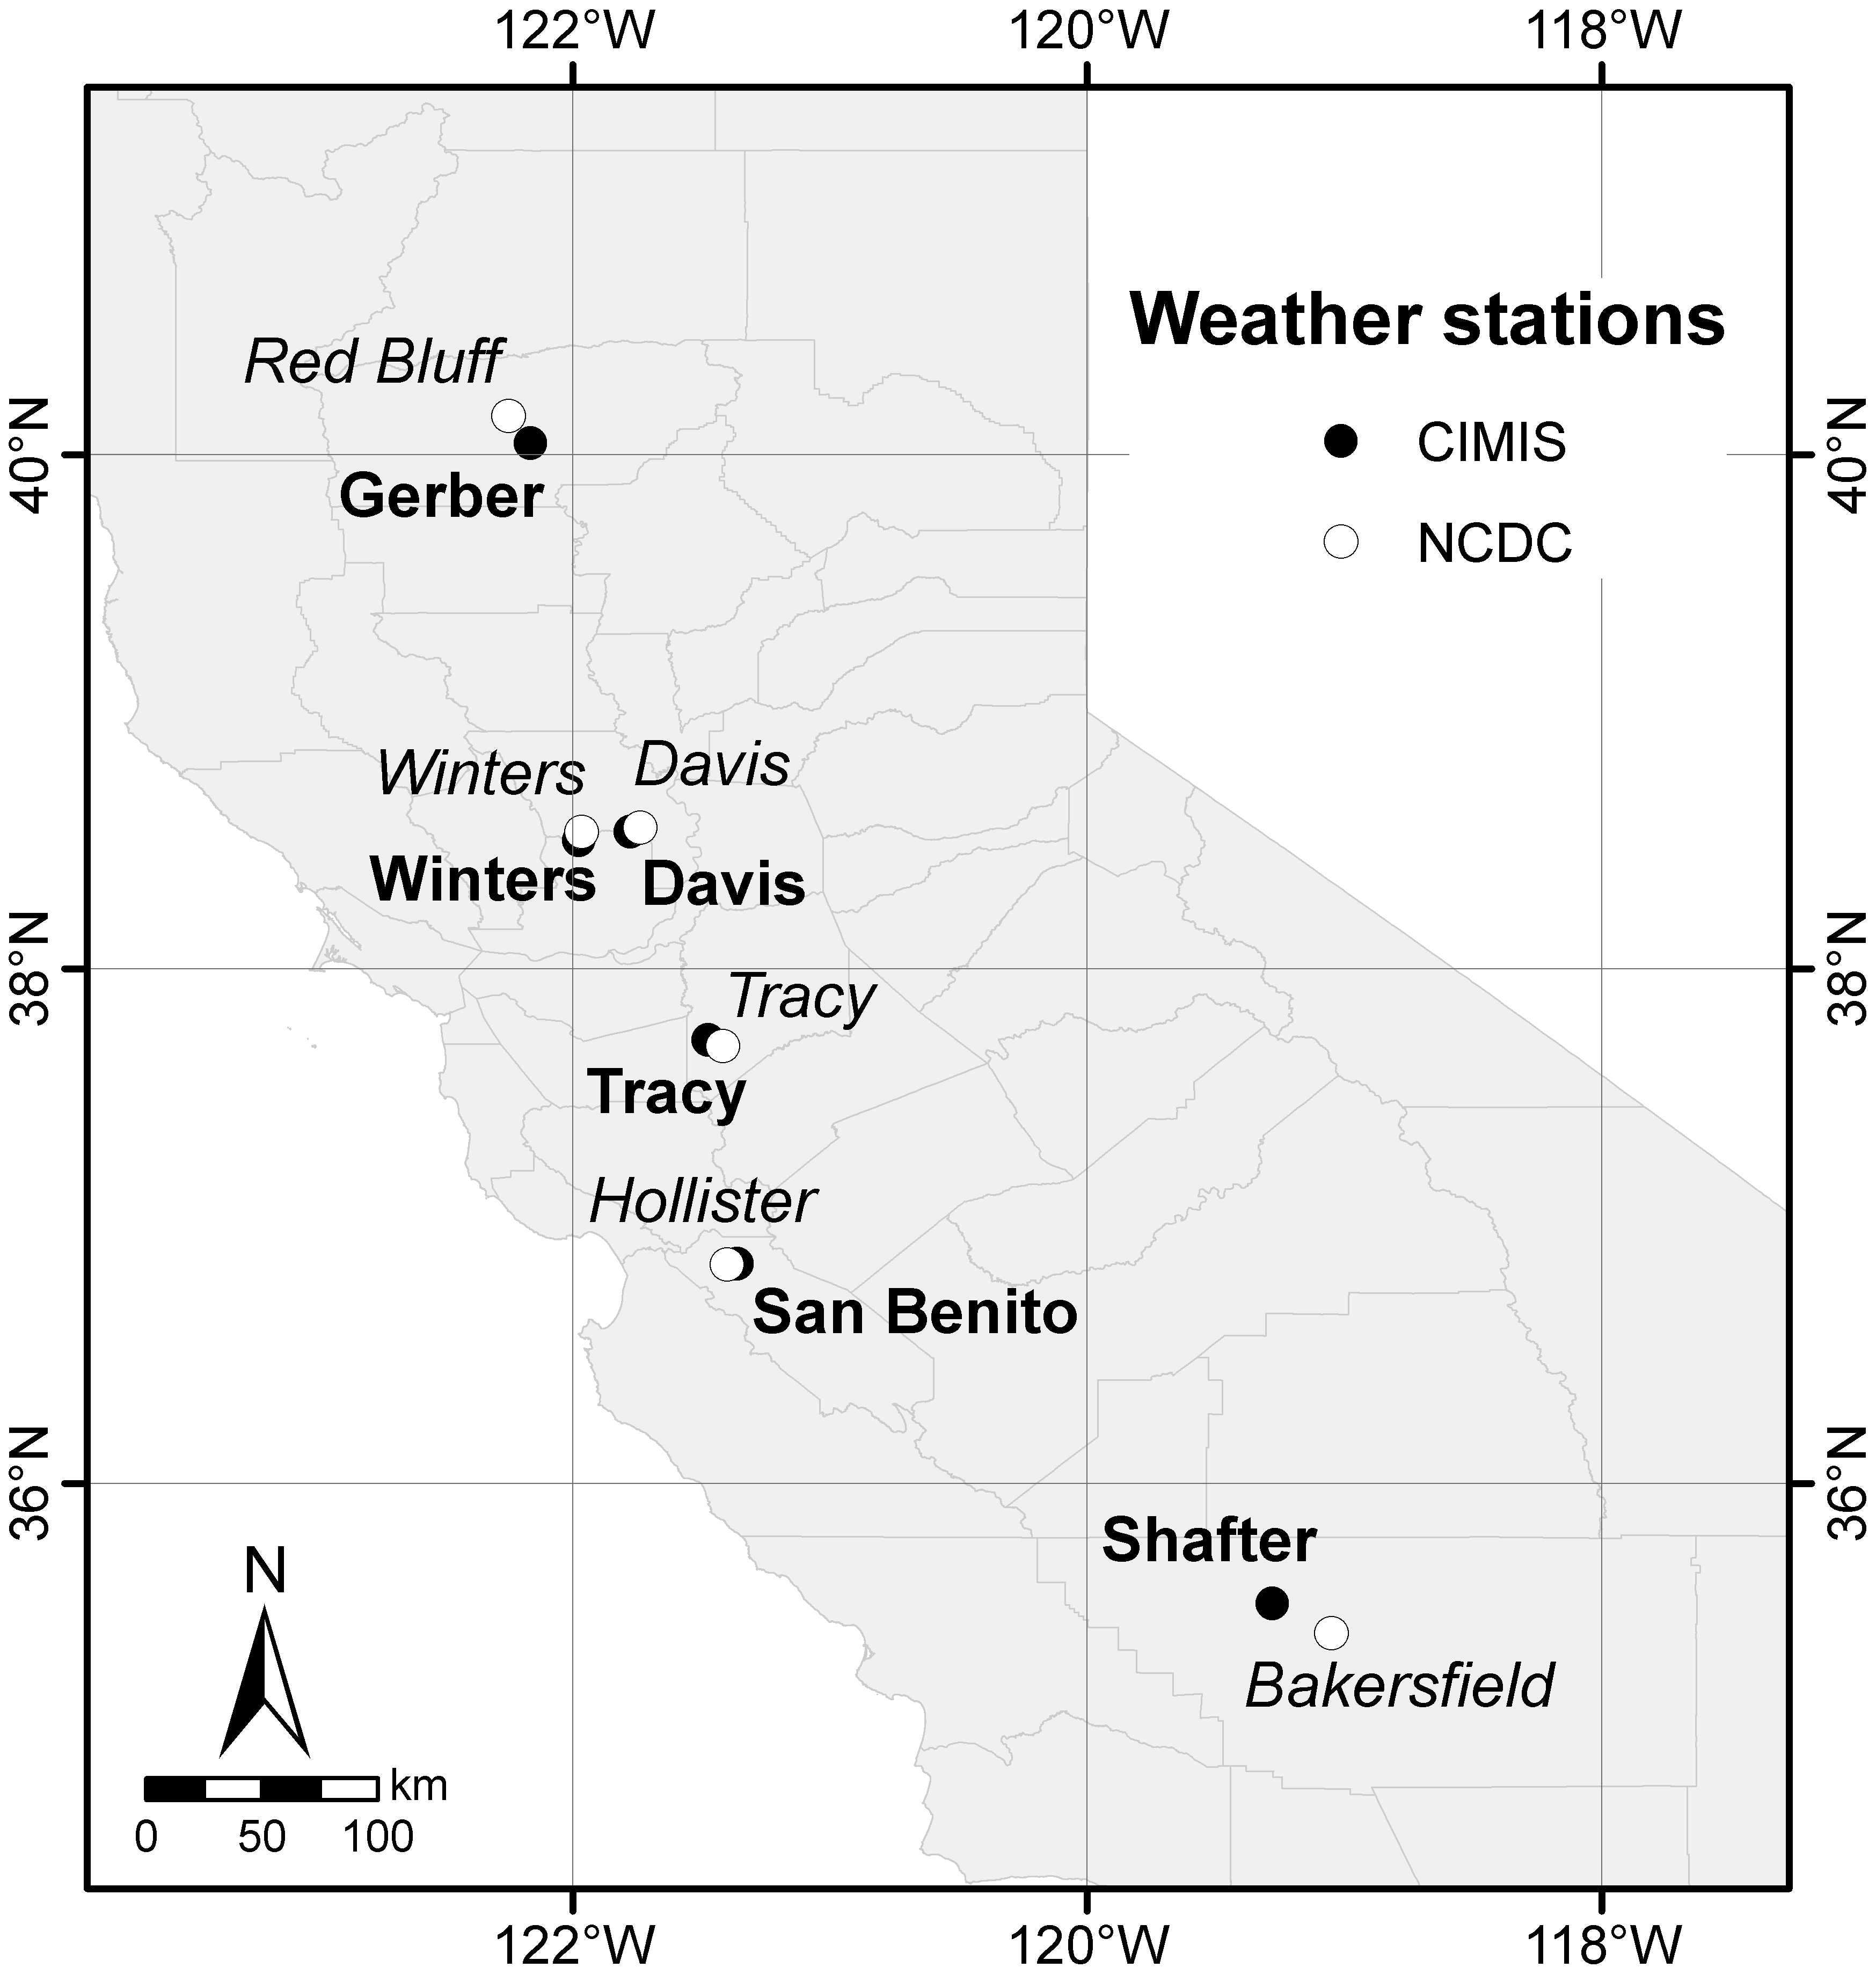
\includegraphics[width=0.9\textwidth,height=\textheight]{pictures/Luedeling_Figure_1.jpg}
\caption{Weather station locations in California}
\end{figure}

Note that `Hollister', a word many people like to display on their clothes in this age we have the privilege of living in, is actually a place in California where people grow walnuts.

Interestingly, the chill projection results varied considerably across the four models I looked at:

\begin{figure}
\centering
\includegraphics[width=0.9\textwidth,height=\textheight]{pictures/Luedeling_Figure_2.JPG}
\caption{Sensitivity of chill projections to model choice (CH - Chilling Hours; Utah - Utah Model; Utah+ - Positive Utah Model; Port. - Dynamic Model)}
\end{figure}

In this figure, the past distribution of winter chill is shown on the left, and estimates for 2000 on the second panel. The remaining three panels show three scenarios for 2050. All data are normalized by the median of the 1950 distribution. You can see that especially by 2050, the models differ strongly in the extent of chill losses they project. Since all models are trying to describe the same thing, this is a strong indication that not all models can be right! This study appeared in Agriculture, Ecosystems and Environment \href{https://www.sciencedirect.com/science/article/abs/pii/S0167880909001248}{(Luedeling, Zhang, Luedeling, et al. \protect\hyperlink{ref-luedeling_sensitivity_2009}{2009})}. I got some welcome help from my brother, who was able to program a little tool to implement the Dynamic Model.

Based on the literature, as well as on another study \href{https://www.sciencedirect.com/science/article/pii/S0168192309001580}{(Luedeling, Zhang, McGranahan, et al. \protect\hyperlink{ref-luedeling2009validation}{2009})} that I don't want to go into here, I concluded that the Dynamic Model was the most reliable one. So this is the model that will be used for the most part in this course.

By the time I did this study, I began to realize that I was running into a few major problems:

\begin{itemize}
\item
  The model that appeared most reliable - the Dynamic Model - was complicated, and I could only calculate Chill Portions (the unit of this model) with a decades-old Excel sheet (Erez and Fishman \protect\hyperlink{ref-ExcelDM}{1997}). This wasn't satisfying.
\item
  Going through the various data processing steps that were needed to produce credible temperature scenarios was cumbersome and error-prone - and boring.
\item
  I was going to have to learn programming\ldots{}
\end{itemize}

\hypertarget{winter-chill-in-california}{%
\subsection{Winter chill in California}\label{winter-chill-in-california}}

The main objective of my stay in California was to produce a winter chill projection for California's fruit and nut growing region - the Central Valley. Here's an impression of what some orchards there look like:

\includegraphics[width=0.45\textwidth,height=\textheight]{pictures/IMG_1087.JPG} 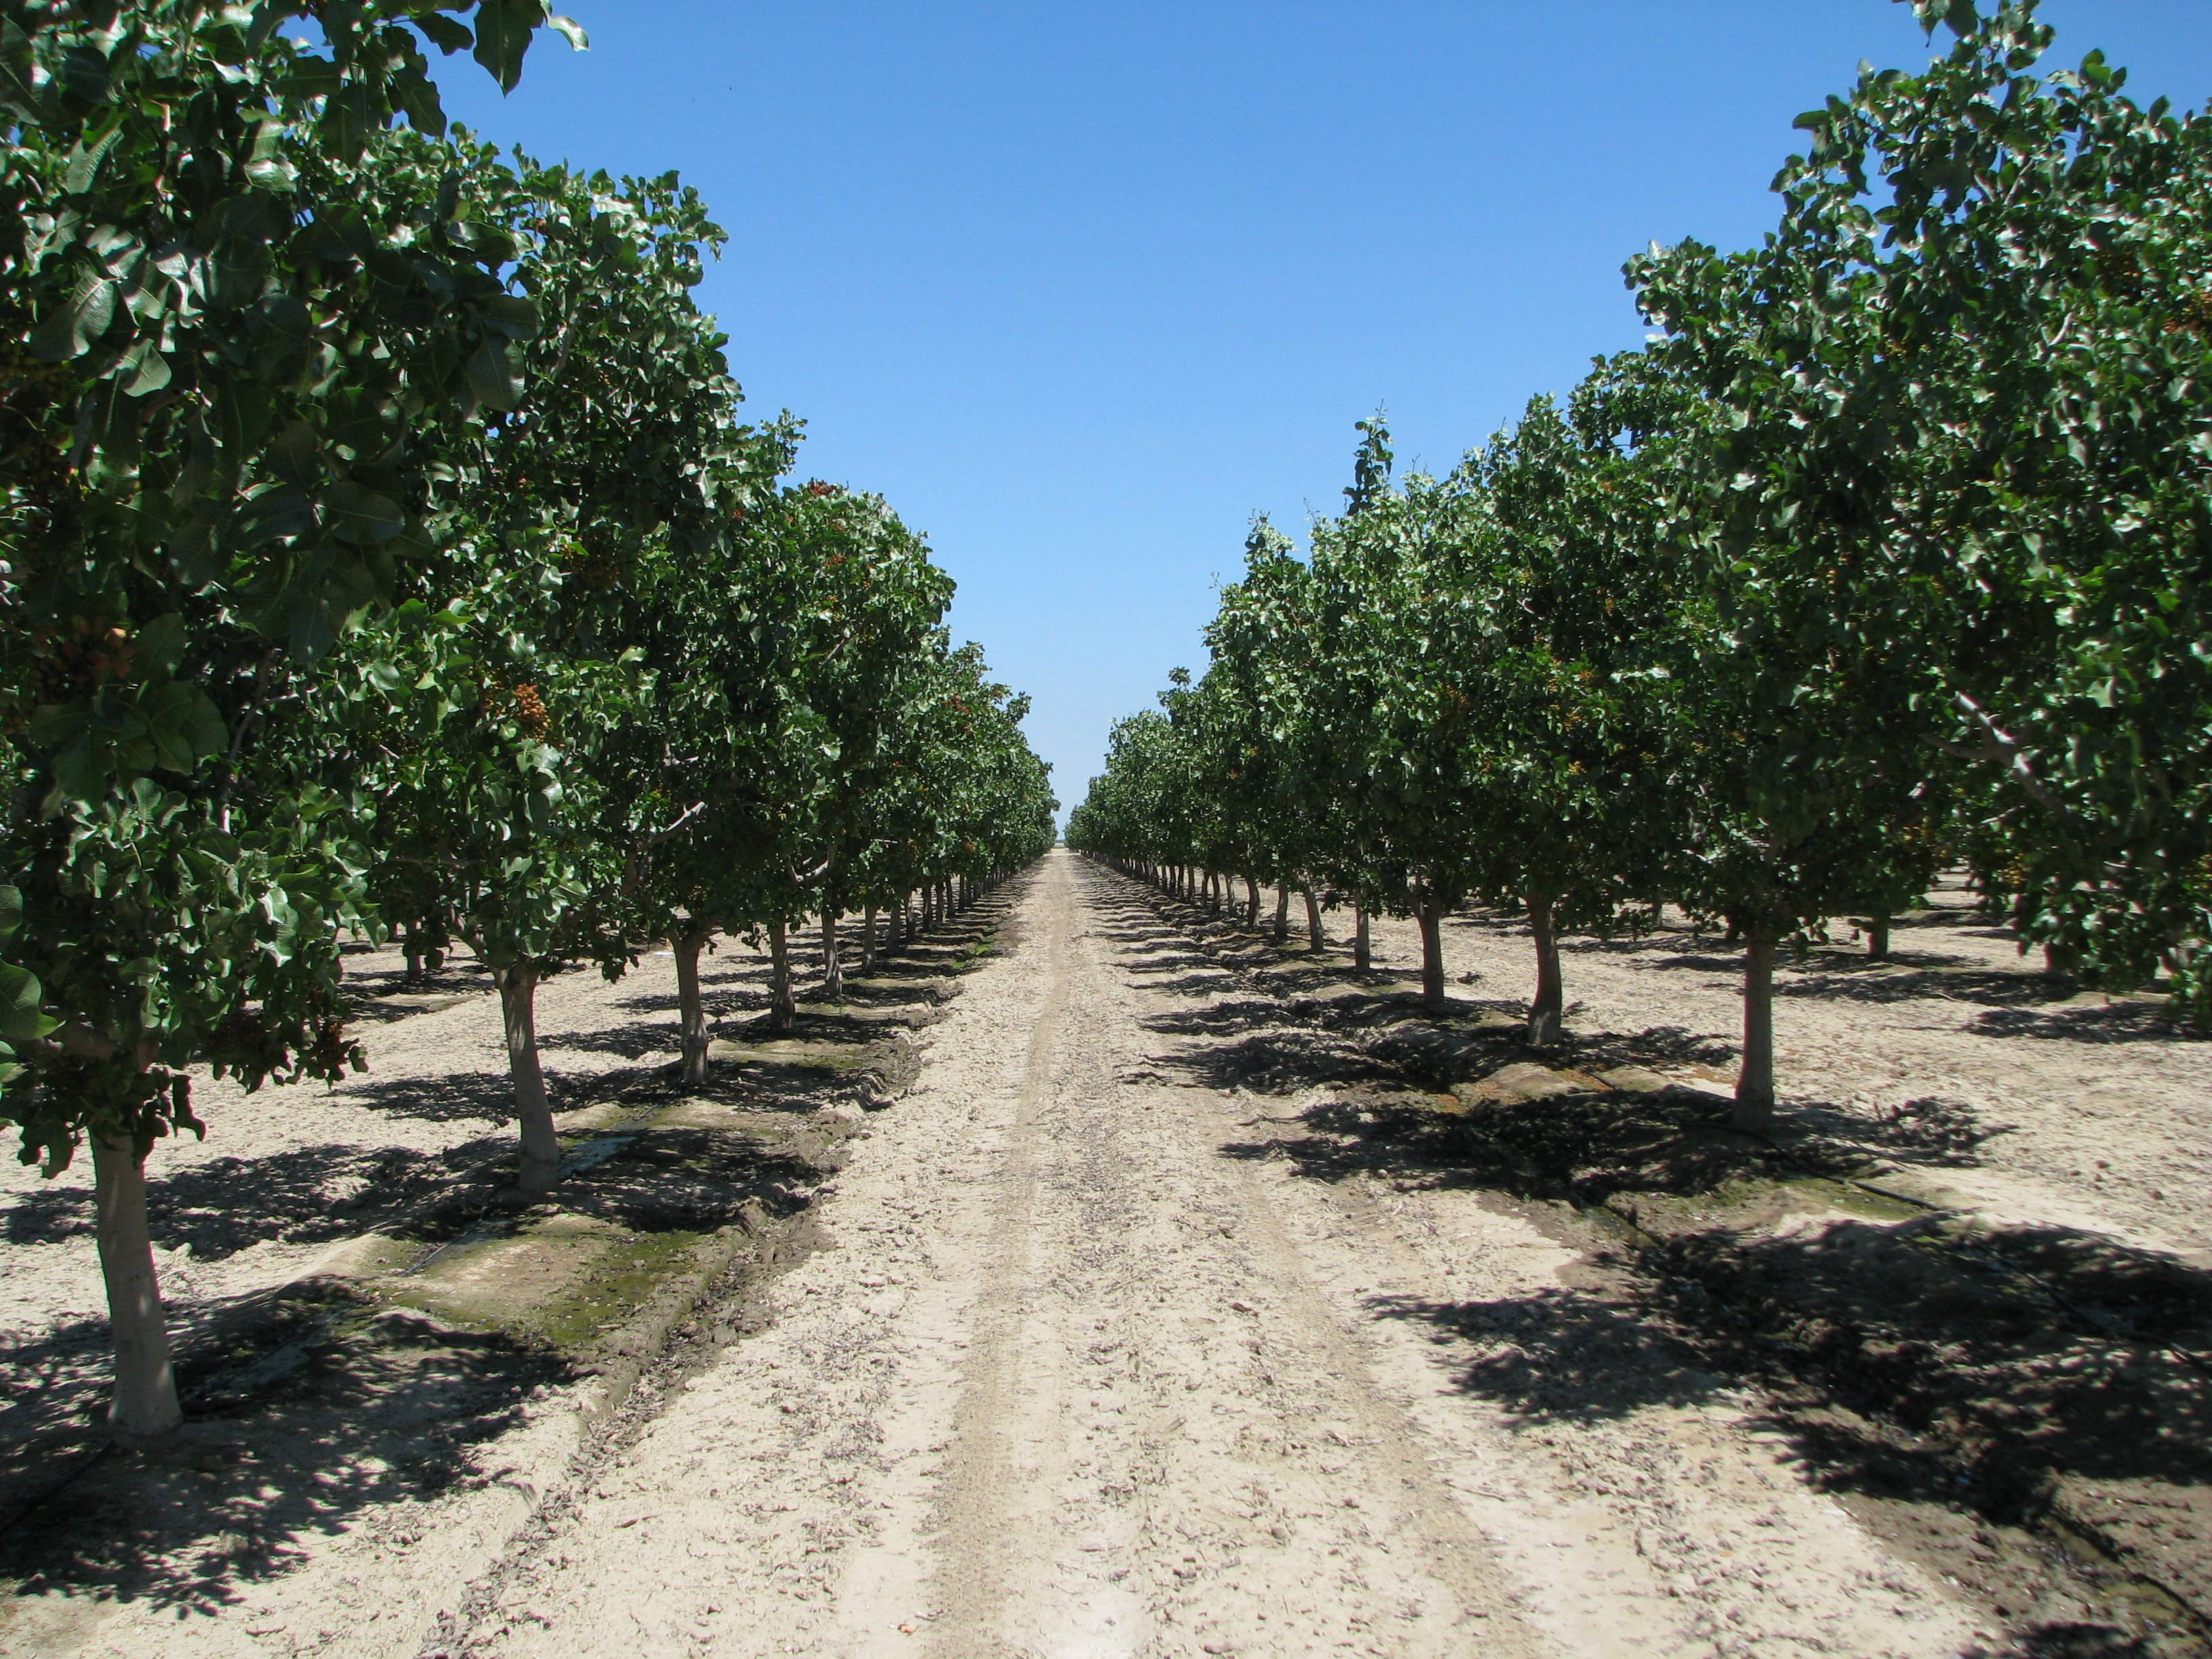
\includegraphics[width=0.45\textwidth,height=\textheight]{pictures/IMG_2969.JPG}

California has a fairly dense \href{https://cimis.water.ca.gov/}{network of weather stations}, and I wanted to use records from all of them. And for all of these 100+ stations, I wanted multiple climate scenarios (20 or so). This was going to take a long time! The only way to deal with this was to automate most of the process, which made me look into programming. For some reasons that now seem like a major mistake, I decided to automate many steps in JSL, the programming language of a statistics program called JMP. While this wasn't a very smart choice, it mostly worked, and I managed to automate most steps. The only step I still had to do manually was run the weather generator (20+ times for each of 100+ weather stations, so this was still pretty annoying\ldots).

In the end, I managed to produce projections for all stations that consisted of chill accumulation over 100 plausible winter seasons per scenario, generated with a weather generator. To condense these results into a format that could be shown in a map, I summarized the data by defining a metric called `Safe Winter Chill'. This is the 10\textsuperscript{th} percentile of the chill distribution, i.e.~the amount of chill that is exceeded in 90\% of all years. Economically, it may be feasible to grow a tree cultivar that requires this much chill. Here's an illustration of the Safe Winter Chill metric:

\begin{figure}
\centering
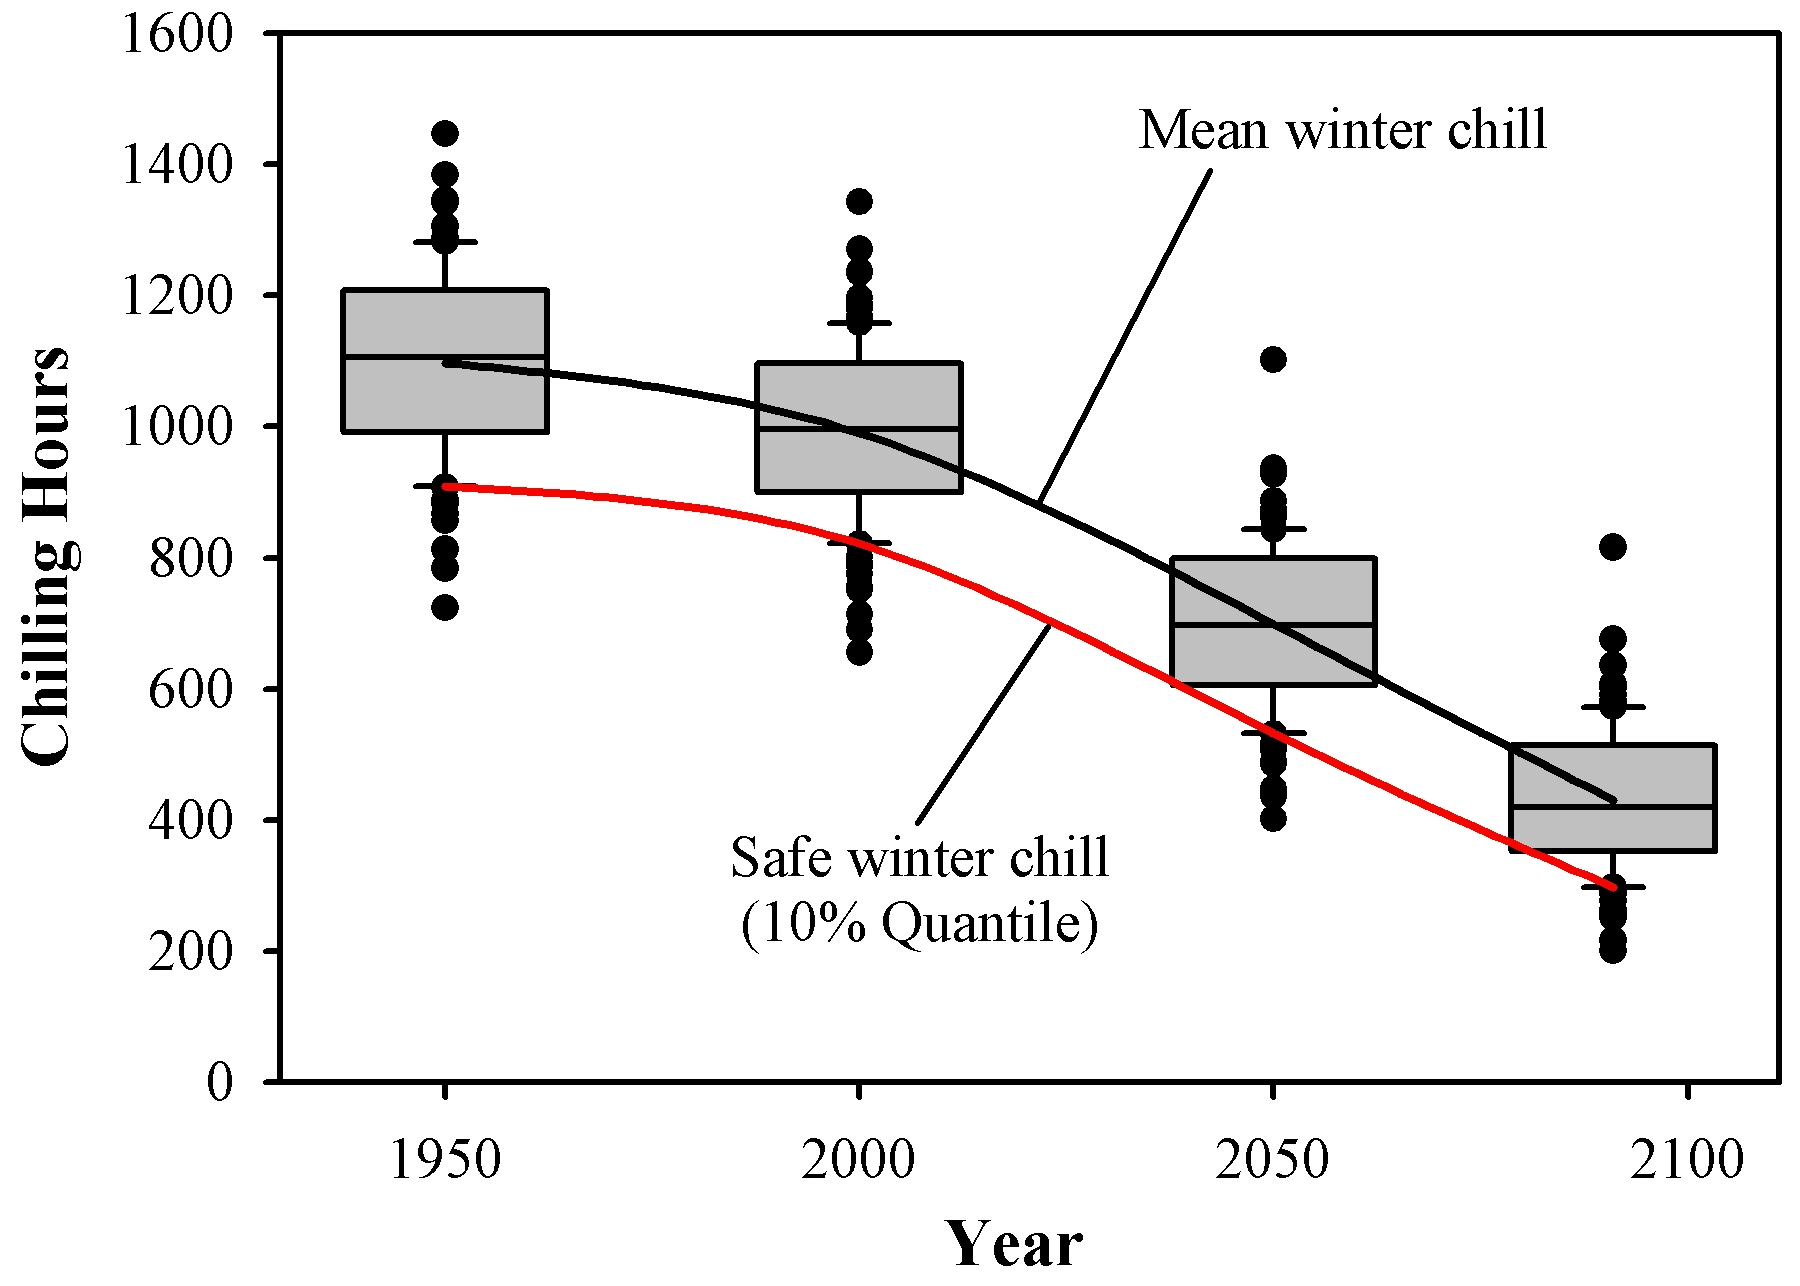
\includegraphics[width=0.9\textwidth,height=\textheight]{pictures/Figure_2_Boxplots_Davis_chilling_hours_a2.JPG}
\caption{Illustration of the Safe Winter Chill concept}
\end{figure}

I also figured out a way to spatially interpolate the station results. We'll get to this later, but here's one of the maps that resulted from this:

\begin{figure}
\centering
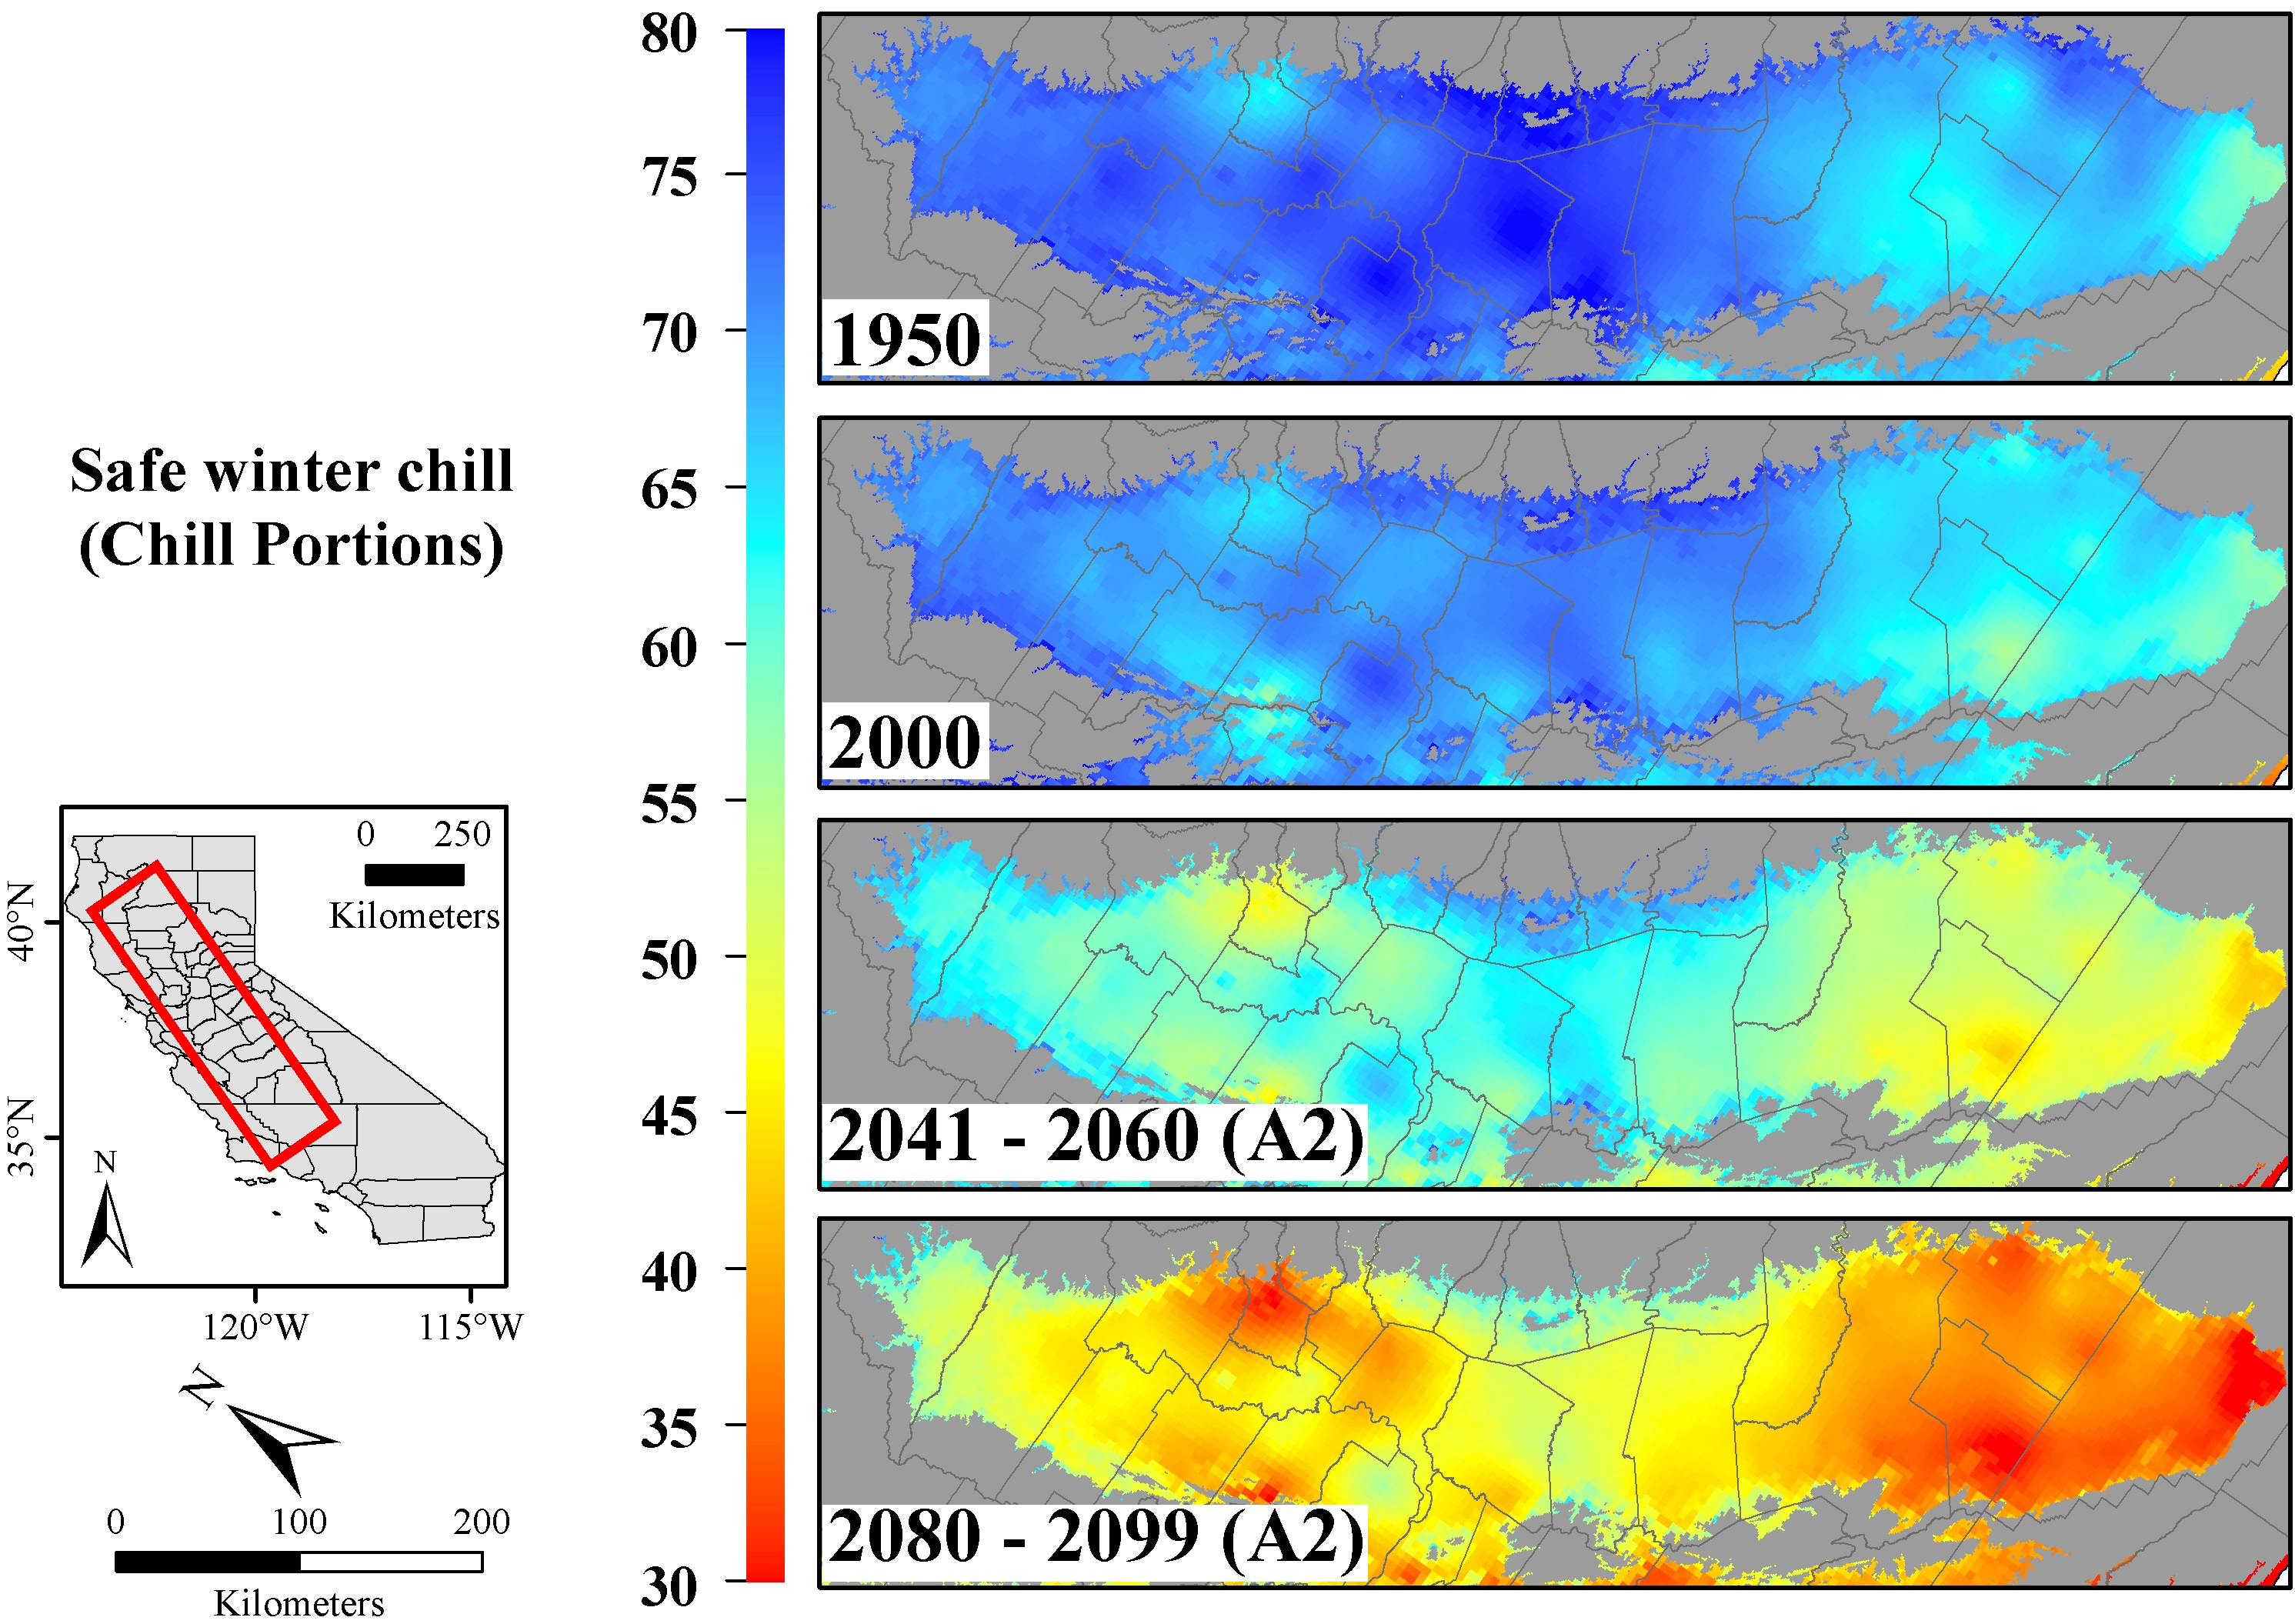
\includegraphics[width=0.9\textwidth,height=\textheight]{pictures/Figure_4_Chill_Portions_Central_Valley_absolute.jpg}
\caption{Winter chill prospects for California's Central Valley}
\end{figure}

This analysis appeared in the journal PLOS ONE \href{https://journals.plos.org/plosone/article?id=10.1371/journal.pone.0006166}{(Luedeling, Zhang, and Girvetz \protect\hyperlink{ref-luedeling_climatic_2009}{2009})} .

\hypertarget{winter-chill-ratios}{%
\subsection{Winter chill ratios}\label{winter-chill-ratios}}

Having figured out how to automate processing steps (in that JSL language), I could move on to greater numbers of stations. The goal was to produce a chill projection for the whole world. I identified a good data source for setting this up in the Global Summary of the Day database (we'll get back to this later). This had useful data for several thousand weather stations (and thousands more of not-so-useful stations, which had to be identified and filtered out). Especially with my fairly poor programming skills, this was a huge endeavor. At some point, the data were being processed on 6 computers, which were running day and night for several weeks. Quite likely, this was not because the analyses were so complex, but because I set things up poorly\ldots{} Anyway, eventually I managed to process data for about 5000 globally distributed weather stations, for which I calculated multiple chill metrics.

This provided an opportunity to compare chill models again. So I calculated, for each weather station in my dataset, the ratio between various chill metrics. Had these ratios been largely constant all over the planet (e.g.~one Chill Portion always corresponds to 10 Chilling Hours), we would have been faily safe using any of the chill models. Unfortunately, this wasn't the case, with enormous variation in chill metric ratios around the world.

\begin{figure}
\centering
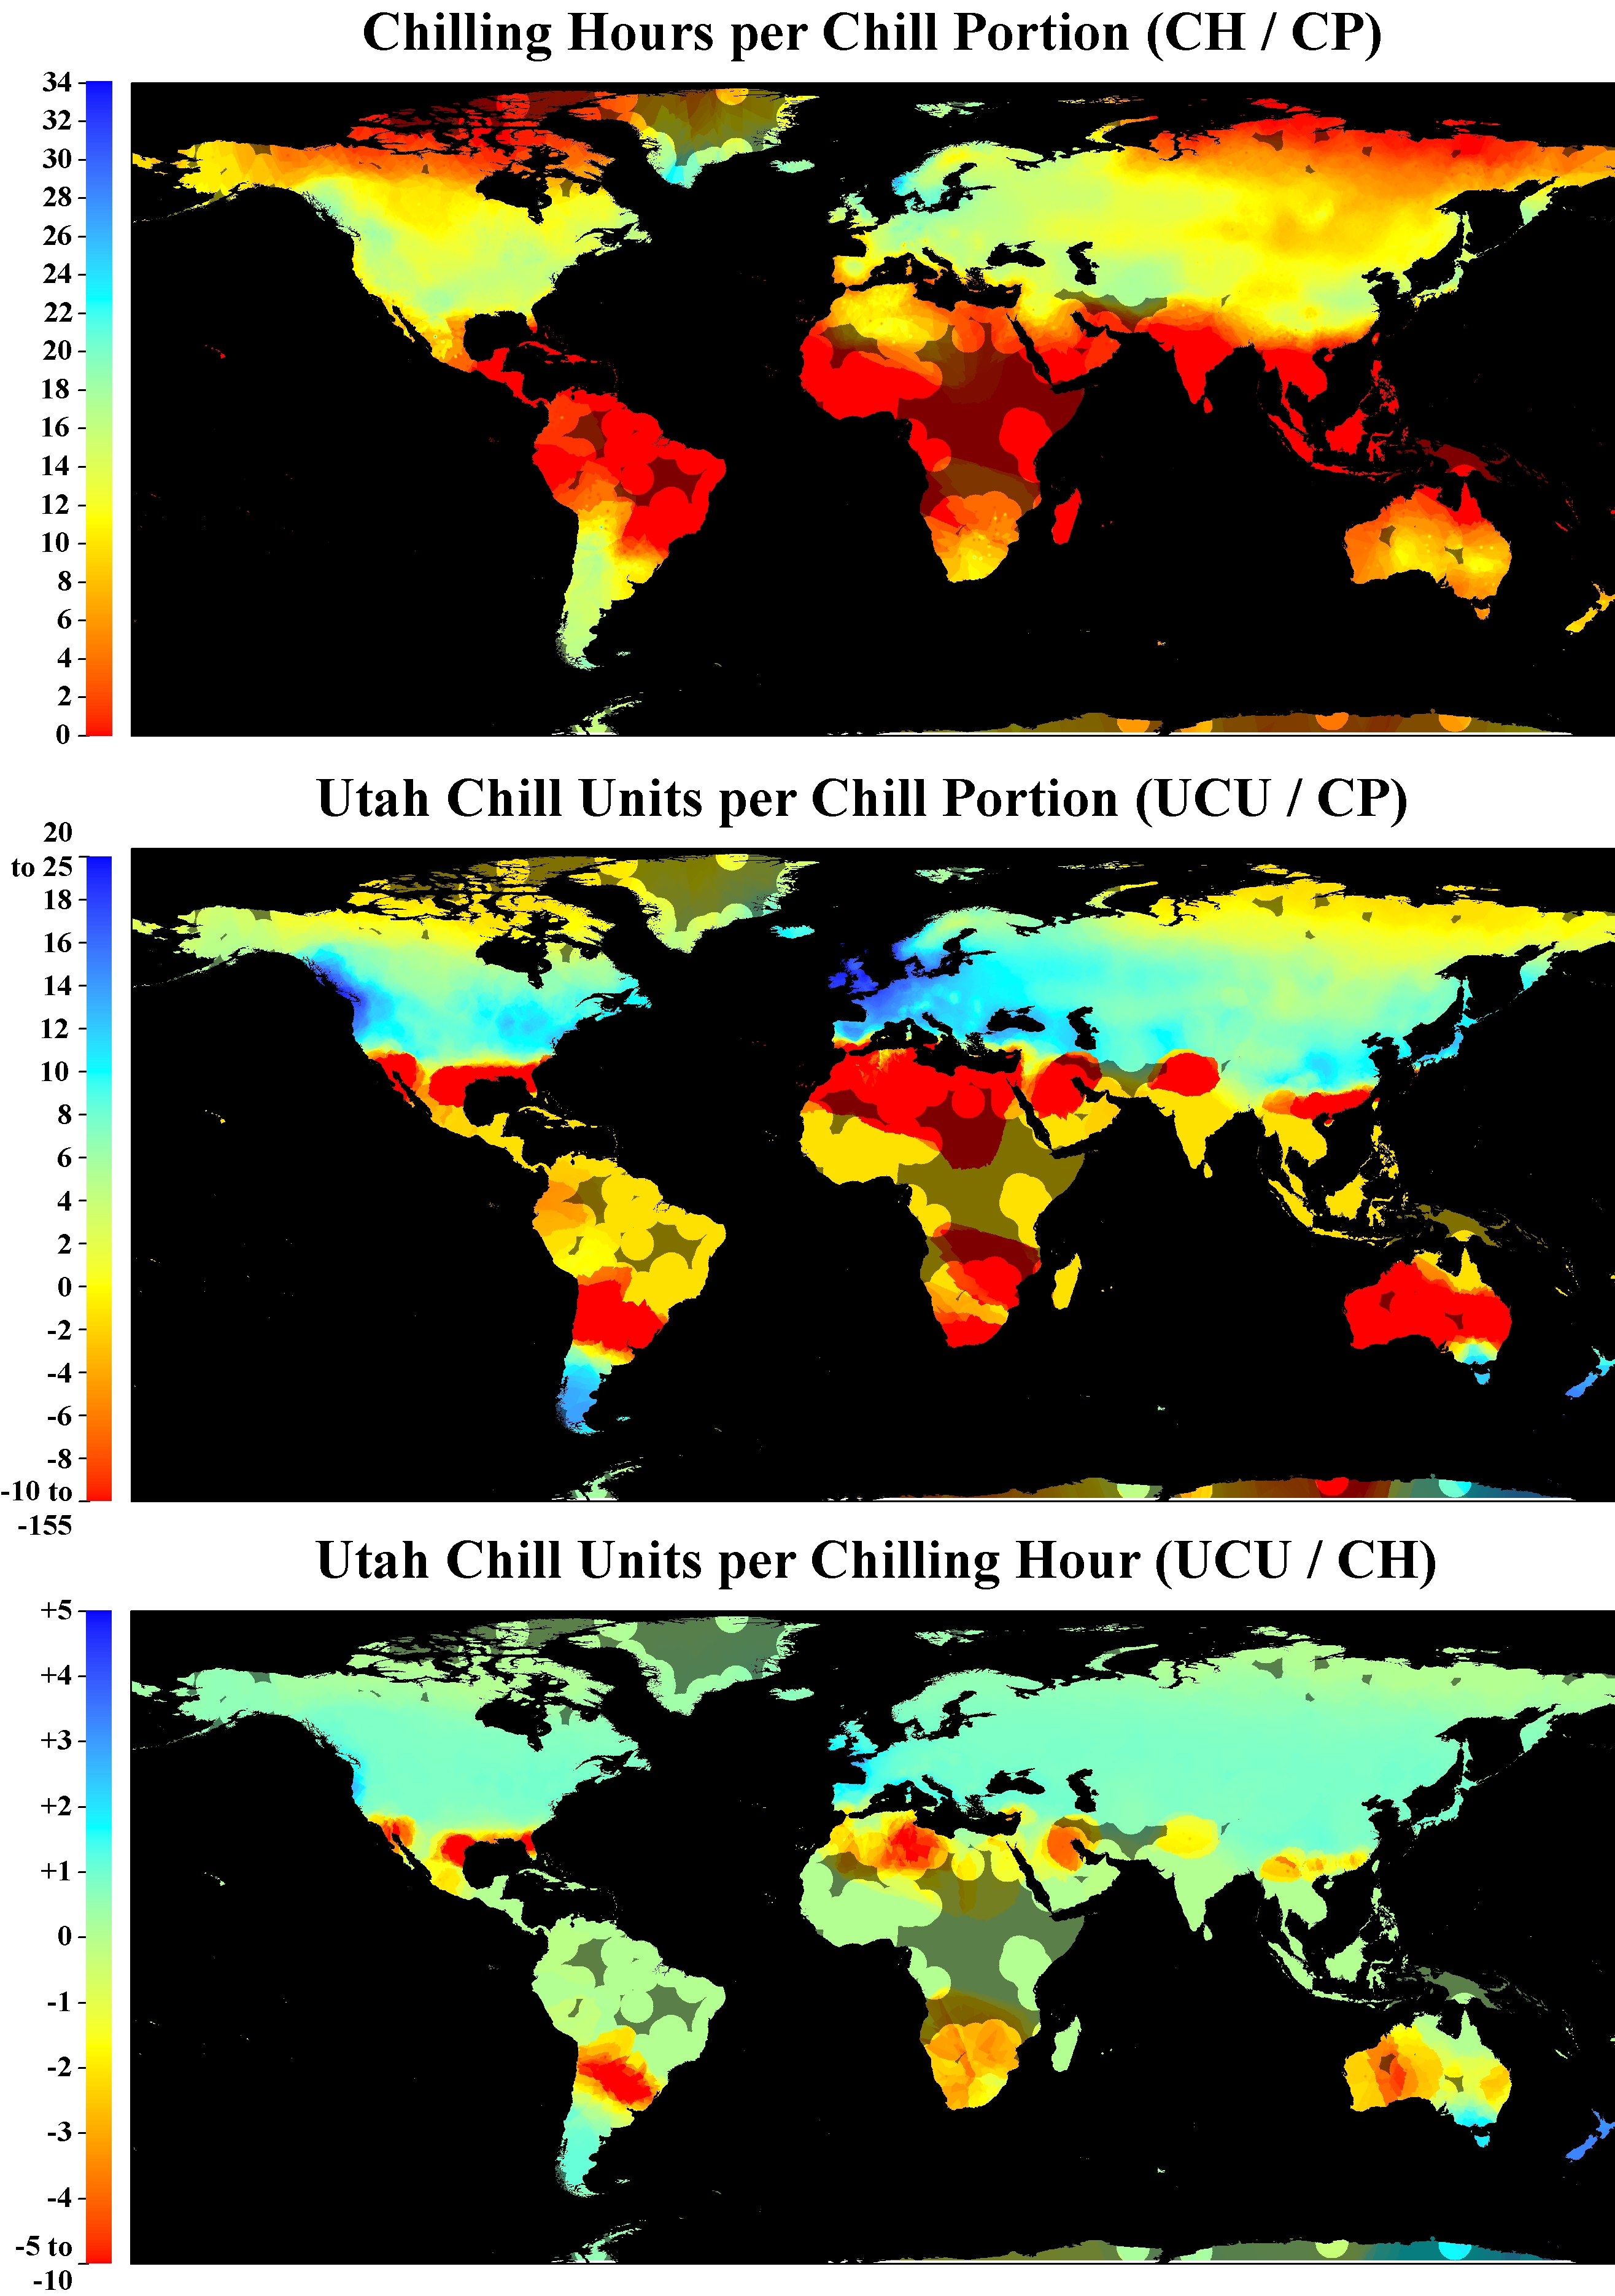
\includegraphics[width=0.9\textwidth,height=\textheight]{pictures/Luedeling_Fig_4_all_ratios_map.jpg}
\caption{Chill metric ratios around the world}
\end{figure}

This study got published in the International Journal of Biometeorology \href{https://link.springer.com/article/10.1007/s00484-010-0352-y}{(Luedeling and Brown \protect\hyperlink{ref-luedeling_global_2011}{2011})}.

\hypertarget{a-global-projection-of-future-winter-chill}{%
\subsection{A global projection of future winter chill}\label{a-global-projection-of-future-winter-chill}}

Based on the same analysis procedures, we were also able to produce a global projection of the likely impacts of climate change on winter chill:

\begin{figure}
\centering
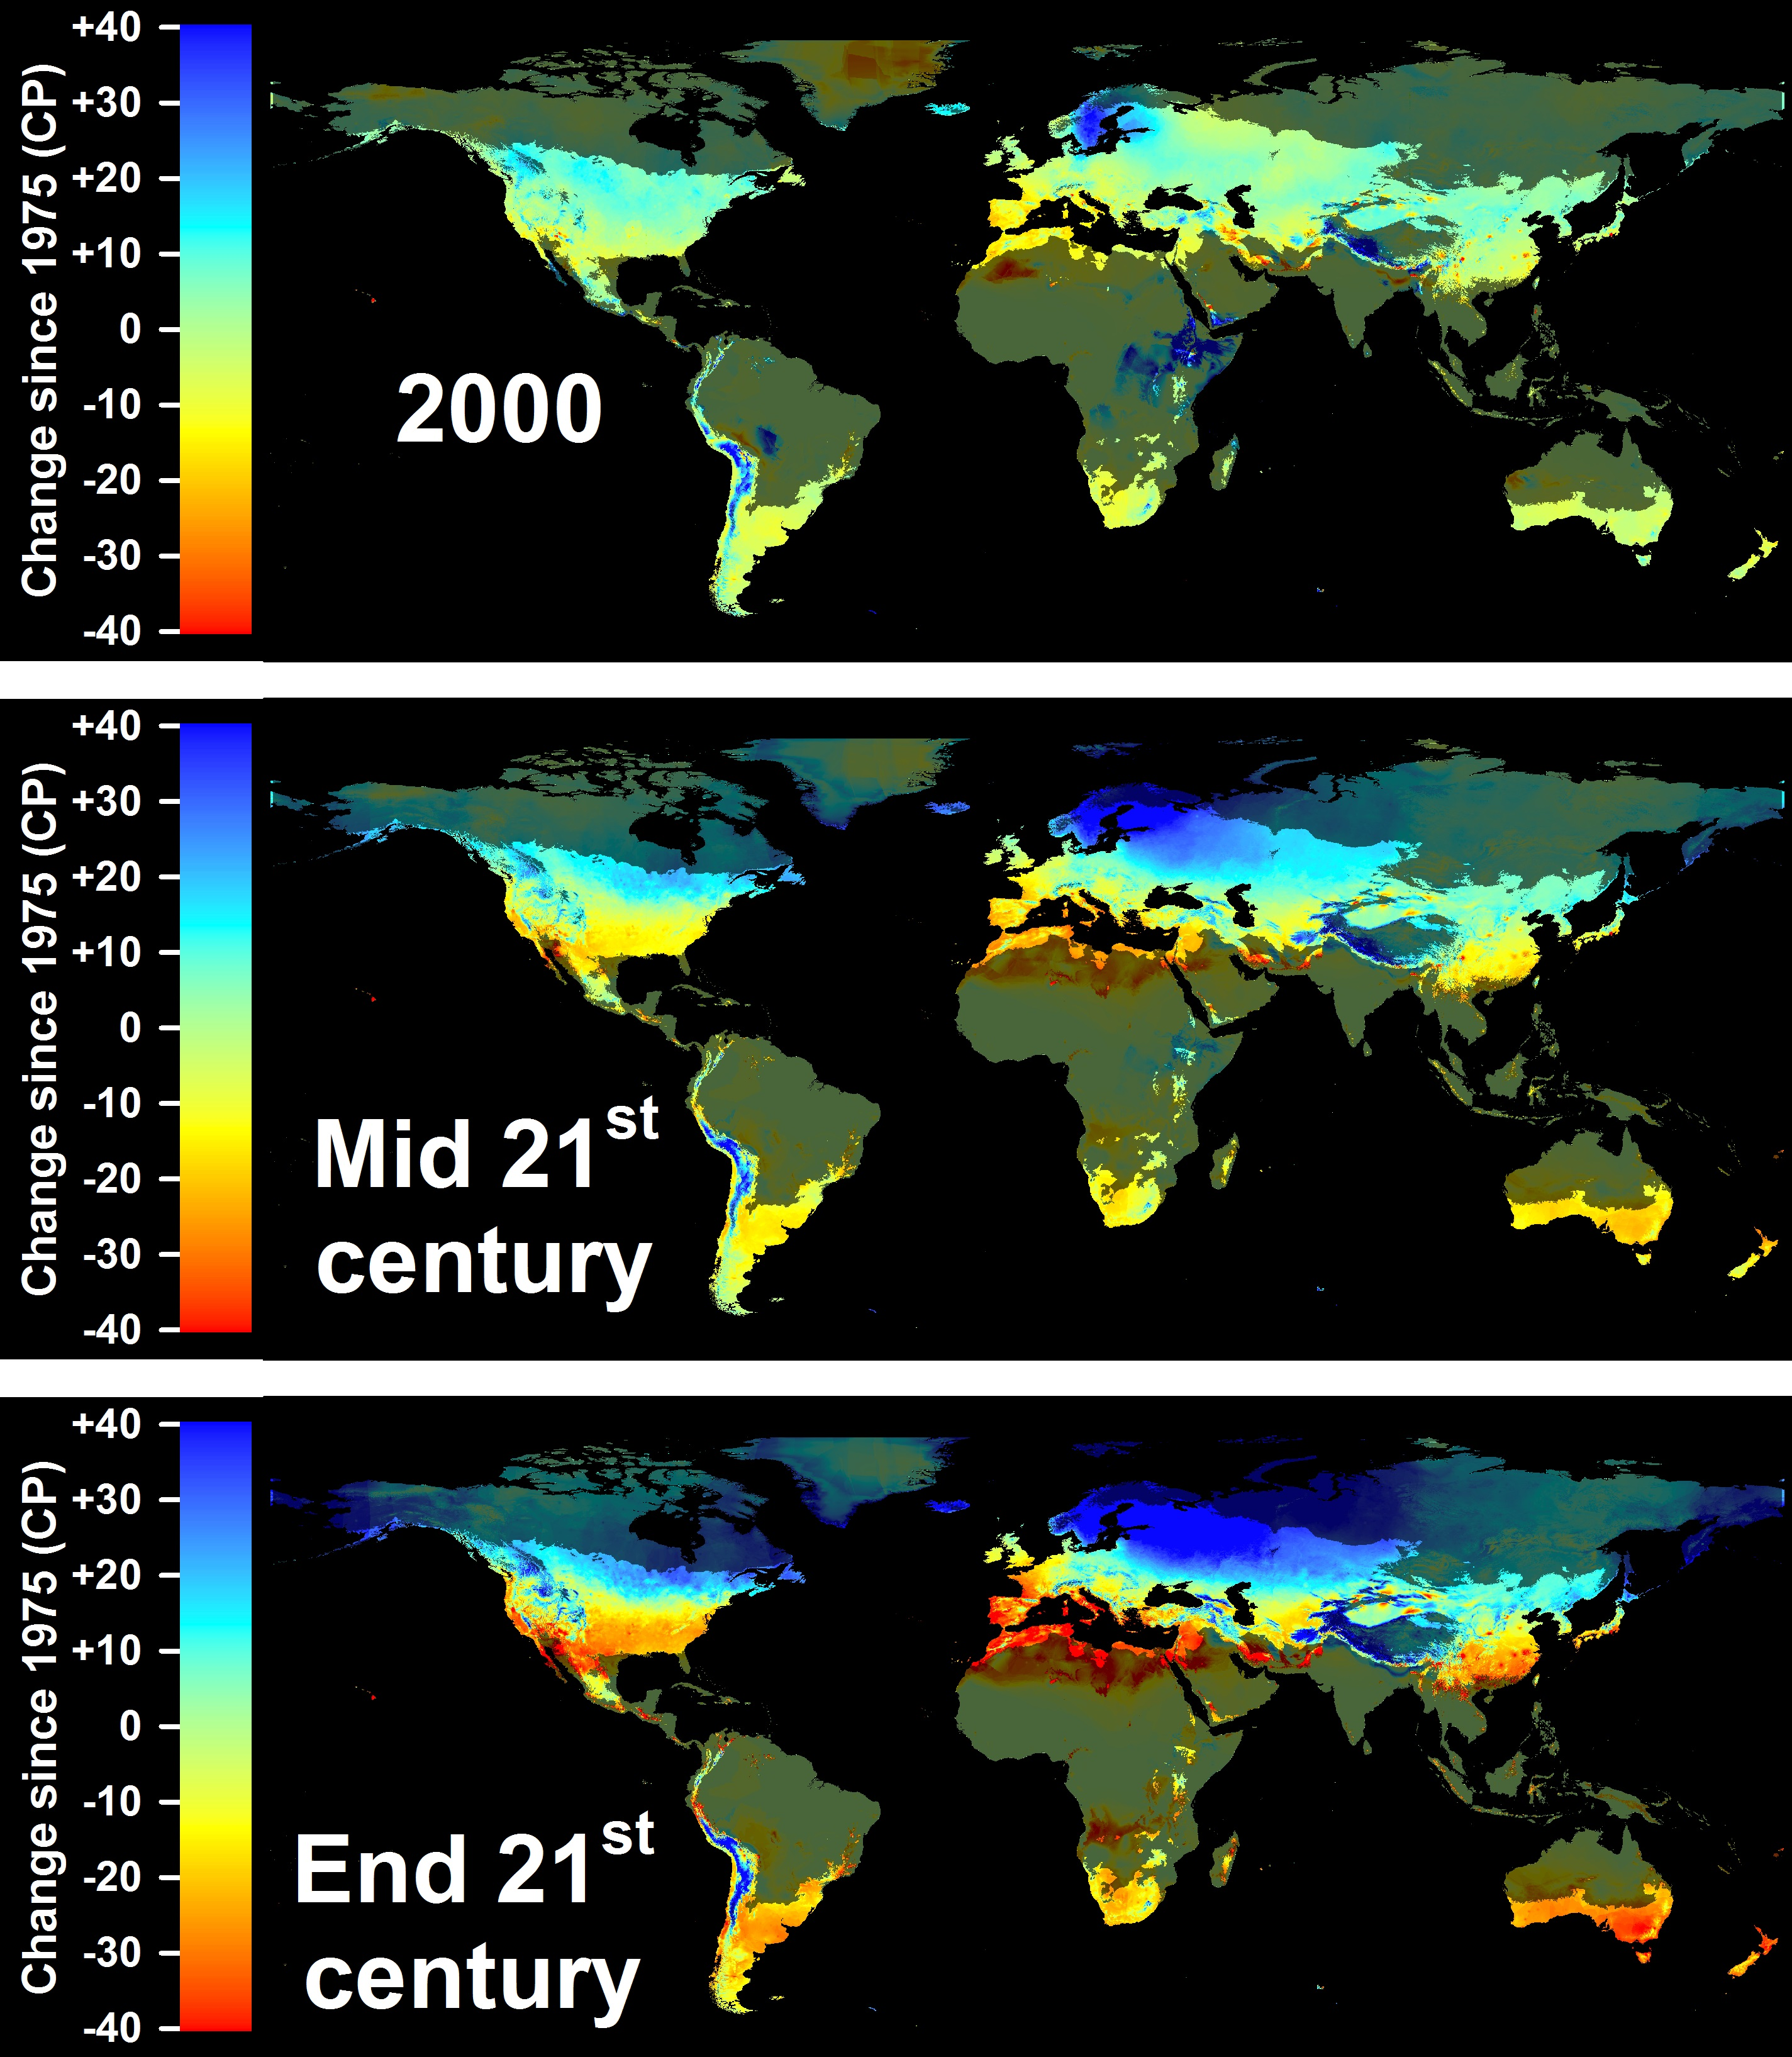
\includegraphics[width=0.9\textwidth,height=\textheight]{pictures/Figure_5_Time_Comp.jpg}
\caption{Projected decline in available winter chill around the world}
\end{figure}

This study was published in PLOS ONE \href{https://journals.plos.org/plosone/article?id=10.1371/journal.pone.0020155}{(Luedeling, Girvetz, et al. \protect\hyperlink{ref-luedeling2011climate}{2011})}.

Especially in the areas shown in red and orange in the lower two maps, fruit and nut production may be quite heavily impacted by declining winter chill. With such dramatic chill losses, it seems unlikely that growers will remain able to grow the tree cultivars they currently rely on. In terms of world regions, the Mediterranean region may be hit particularly hard.

\begin{figure}
\centering
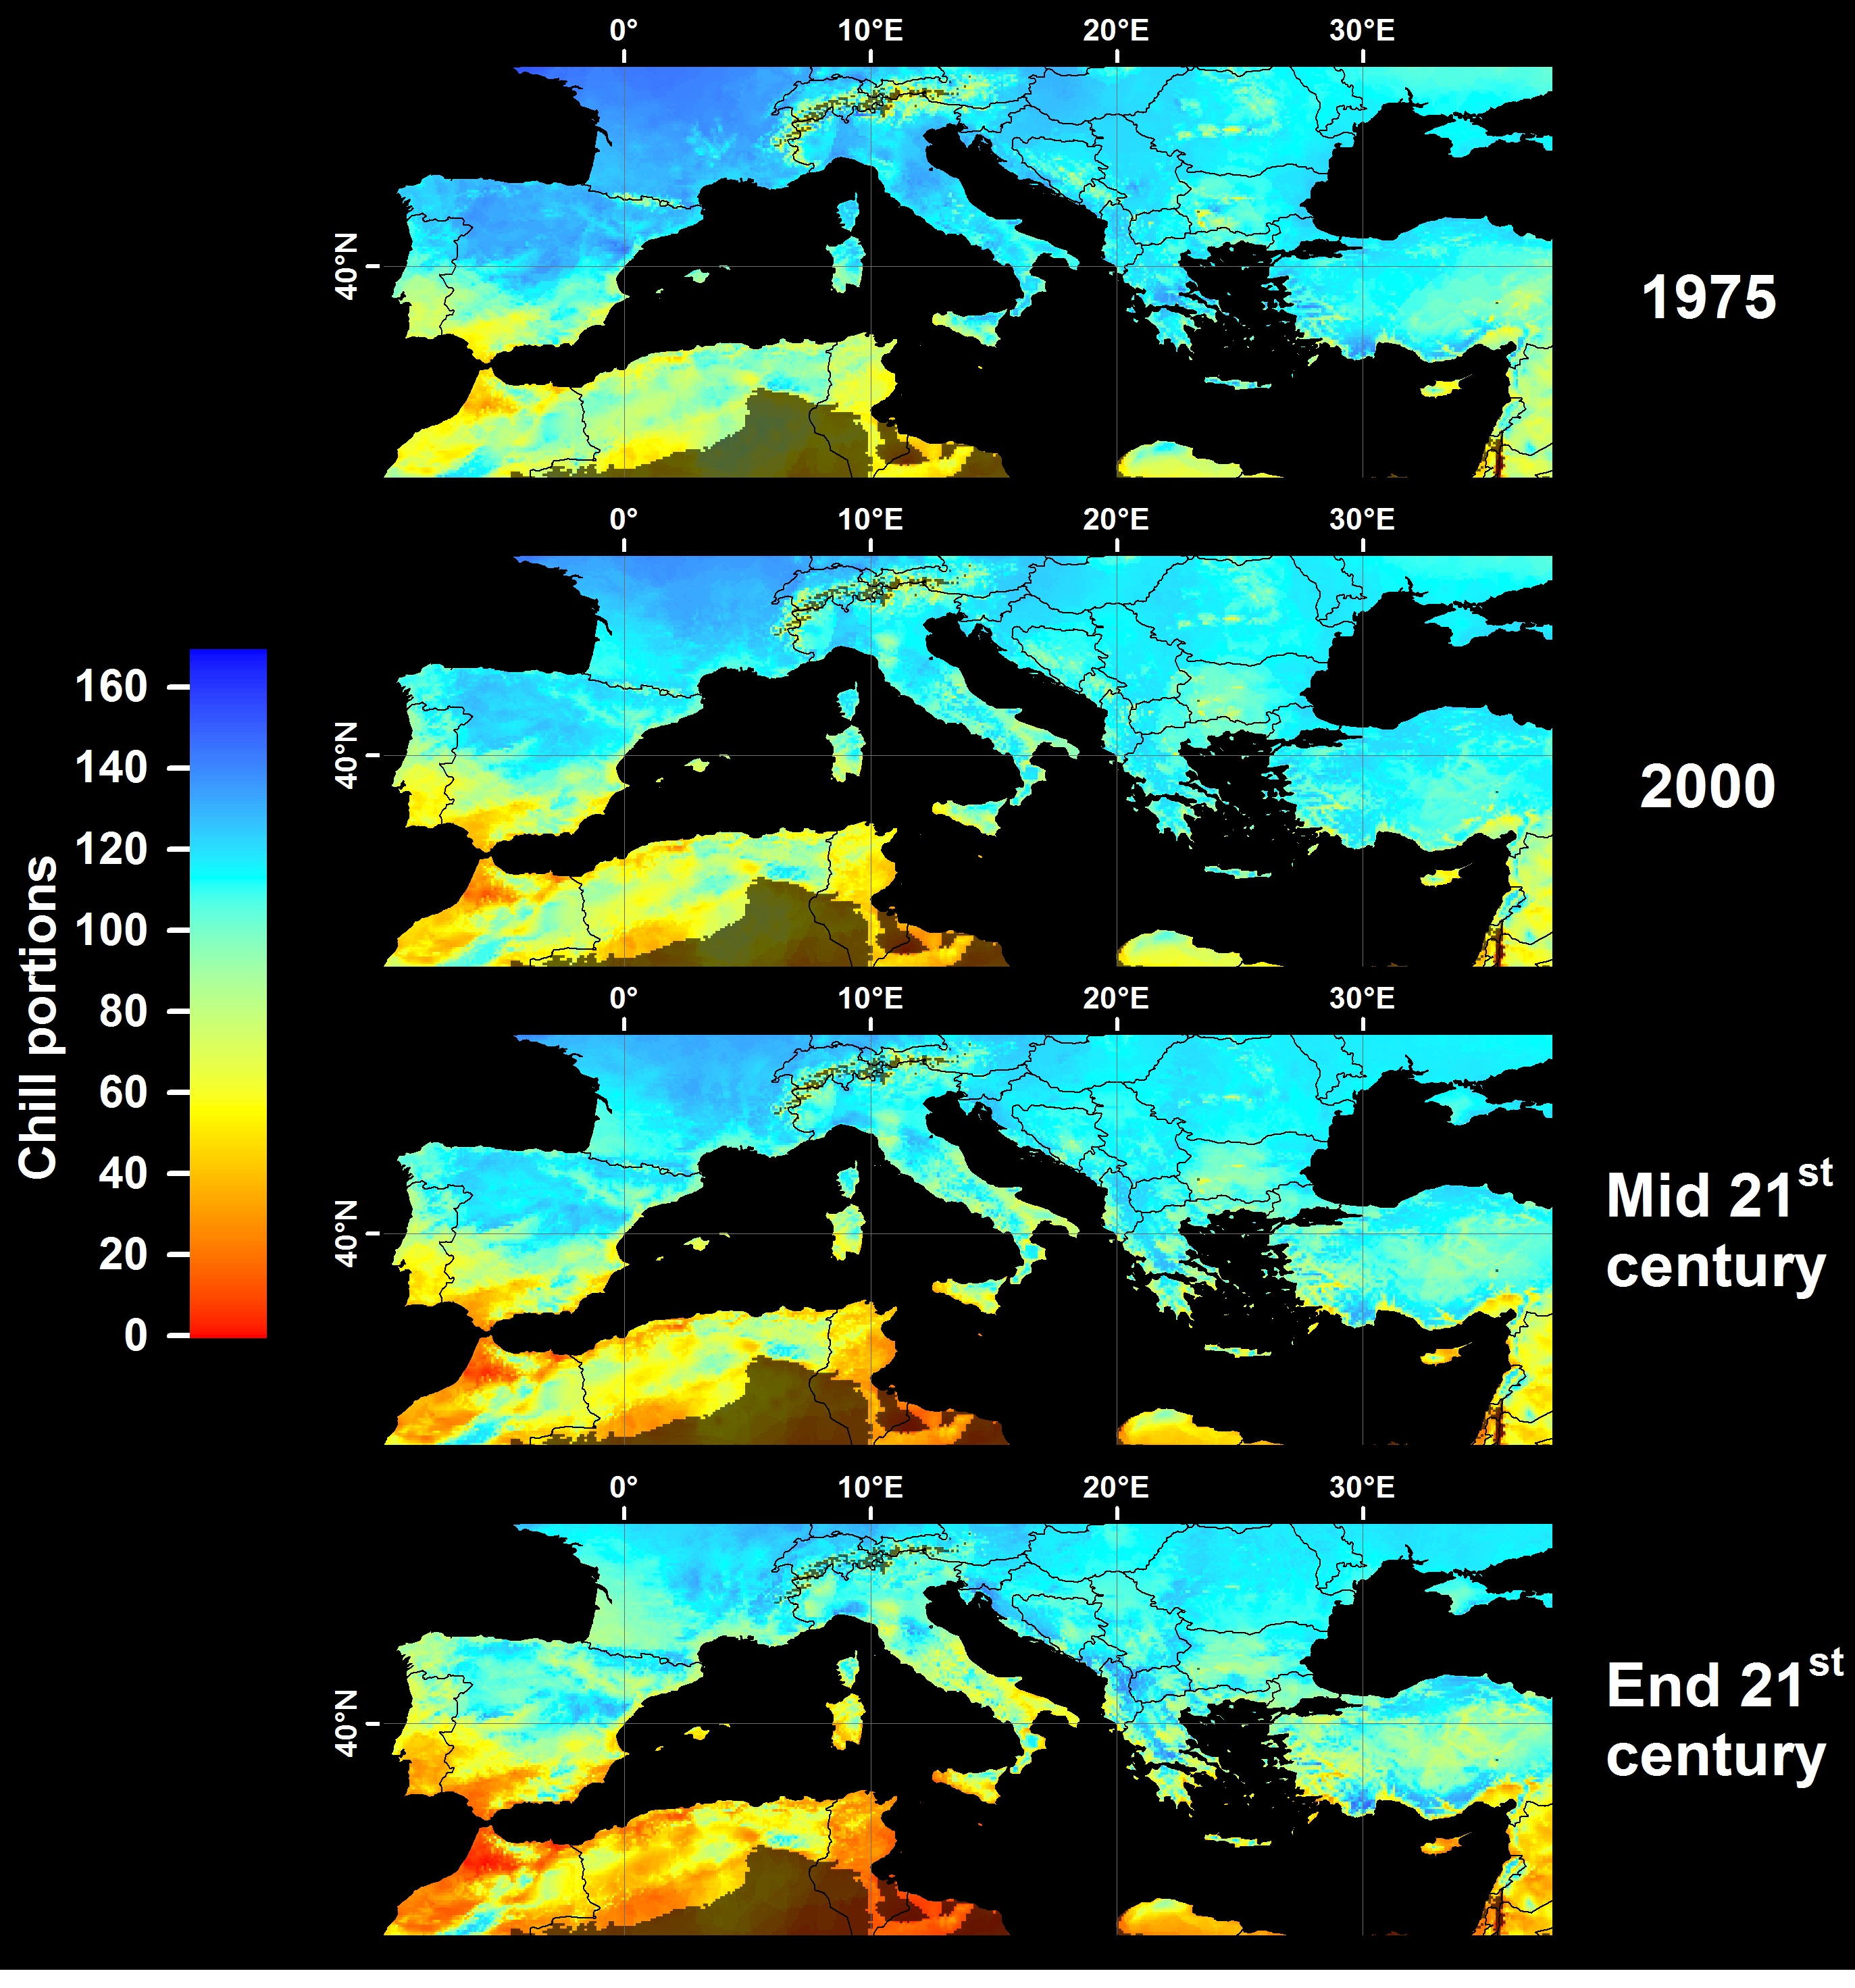
\includegraphics[width=0.9\textwidth,height=\textheight]{pictures/Figure_6_regional_grids_Mediterranean.jpg}
\caption{Winter chill projection for the Mediterranean region}
\end{figure}

This is one of the reasons why we started working with partners in this region, as well as other countries with similar climatic settings (e.g.~South Africa, Chile).

\hypertarget{winter-chill-in-germany}{%
\subsection{Winter chill in Germany}\label{winter-chill-in-germany}}

Germany is not highlighed as particularly vulnerable to chill losses. Analyzing historic chilling trends between 1950, we were able to confirm this impression \href{https://link.springer.com/article/10.1007/s10341-009-0085-4}{(Luedeling, Blanke, and Gebauer \protect\hyperlink{ref-luedeling_auswirkungen_2009}{2009})}.

\begin{figure}
\centering
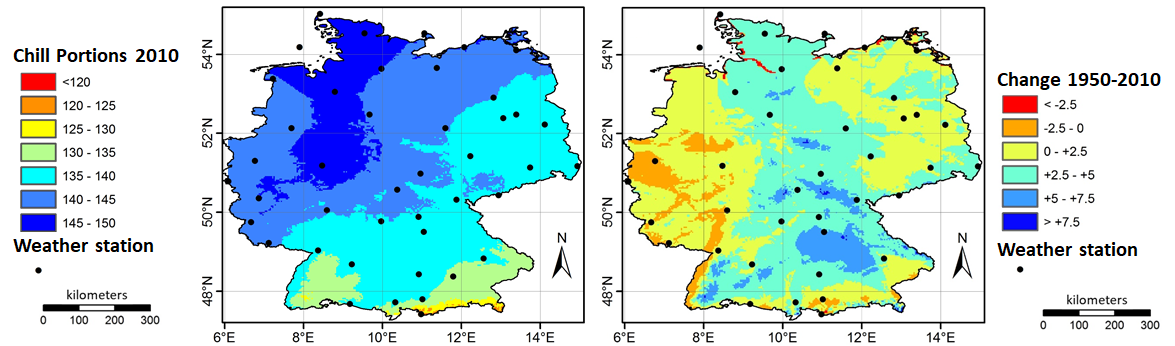
\includegraphics[width=0.9\textwidth,height=\textheight]{pictures/Chilling_Germany.png}
\caption{Winter chill in Germany in 2010, and changes between 1950 and 2010}
\end{figure}

The reason for this lack of major changes is that current winter temperatures in Germany are right in the middle of what appears to be the most effective temperature range for chill accumulation. A little warmer or a little colder therefore doesn't make much of a difference.

\hypertarget{winter-chill-in-tunisia}{%
\subsection{Winter chill in Tunisia}\label{winter-chill-in-tunisia}}

Prospects are quite different for orchards in Tunisia. Here we're close to the warmest margin of the production range for many fruit and nut tree species. We published an assessment of past and future trends in winter chill for an orchard in Central Tunisia in 2018, about 7 years after all the other projection studies shown above. This long break was partly because my day job at the time involved \href{https://www.worldagroforestry.org/}{agroforestry}, \href{https://thesolutionsjournal.com/2016/09/17/decision-focused-agricultural-research/}{decision analysis} and a few other things, but not winter chill. More importantly, however, it took me quite a while to overcome a major challenge of climate change analysis - where to find appropriate information on future climates.

Difficulties in finding future climate data may seem surprising, given the ubiquity of climate change research. In fact, finding data is not difficult, but data that can easily be used for the purposes of chill modeling (of the kind I like doing) still wasn't readily available. For some reason, most future climate projections were mostly disseminated as spatial grids covering various extents. Some datasets were only within my reach as raster files covering the whole planet. At even a moderate spatial resolution of 2.5 arcminutes, each of these grids had a size of about 170 MB. This may not sound like much, but consider that for each climate scenario, we need 12 grids for the mean daily minimum temperature of each month, and another 12 for the maximum temperature (for some weather generators, we need another 12 for rainfall). Consider further that for state-of-the-art climate change scenarios, we should investigate multiple future climate `pathways'. In my earlier studies, we used the so-called SRES emissions scenarios (named after the IPCC \textbf{S}pecial \textbf{R}eport on \textbf{E}missions \textbf{S}cenarios), usually focusing on the three most commonly used scenarios B2, A1B and A2. So now we're already at 72 grids (assuming we don't need rainfall).

Since we still have incomplete understanding on how the global climate system works, many research groups have developed so-called `General Circulation Models' (GCMs; many people also use an alternative long form: `Global Climate Models'), all of which differ slightly in their projections. We currently have no way of deciding which of these models, if any, is right, so the climate science community decided that we should produce \emph{ensemble} forecasts, i.e.~project changes using outputs from all the available models (that are considered credible). The dataset I typically worked with included 20 GCMs. To make matters worse, I typically wanted to project gradual changes over time by including multiple years in an analysis, e.g.~the 2020s, the 2050s and the 2080s. You can probably see where this is headed. When we multiply all these numbers, we realize that we need 4320 grids. The disk space required to store these data (in uncompressed form) is more than 700 GB. This is not impossible to find, but processing this amount of data is cumbersome and time-consuming. Still, I actually managed to set up a data processing structure for this and download all the data to an external hard drive.

Soon after I had set up this structure, the IPCC came up with a new report that introduced the `Representative Concentration Pathways' (RCPs) to replace the SRES scenarios. For a few years, it was still ok to work with the old scenarios, but eventually it got harder and harder to get such studies through the peer-review process. The scenarios simply weren't up to date any more. However, I was not excited by the prospect of downloading another massive dataset and starting all over again\ldots{} What made this particularly difficult for me was that I was based in Kenya then, with fairly poor data transfer rates.

It was only until I started working with colleagues in Tunisia, specifically with \href{https://scholar.google.de/citations?hl=de\&user=DdV9jsAAAAAJ}{Haifa Benmoussa}, who was doing her PhD at the University of Tunis, but collaborated intensively with me on most of her dissertation chapters. In some of these chapters, we discovered that tree crops grown in Central Tunisia, specifically almonds \href{https://www.sciencedirect.com/science/article/pii/S0168192317300734}{(Haı̈fa Benmoussa et al. \protect\hyperlink{ref-benmoussa2017chilling}{2017})} and pistachios \href{https://www.sciencedirect.com/science/article/abs/pii/S0098847217301119}{(Haïfa Benmoussa et al. \protect\hyperlink{ref-benmoussa_performance_2017}{2017})} were highly vulnerable to the impacts of climate change. In order to forecast the future prospects for pistachios and almonds in Tunisia, we needed climate scenarios.

It turned out that in the meantime, some climate scientists had produced a future climate database specifically for Africa - AFRICLIM (Platts, Omeny, and Marchant \protect\hyperlink{ref-platts2015africlim}{2015}), which contained exactly what we needed. Since this database didn't include the whole planet, it was much easier to download and store, and processing the data was much less cumbersome. So I added functions to \texttt{chillR} to implement procedures to sample from the AFRICLIM grids and produce \emph{ensembles} of climate scenarios. I also started putting together a framework to automatically produce the kind of plots that are shown below. Here's the plot we produced for this paper \href{https://link.springer.com/article/10.1007/s00484-018-1628-x}{(Benmoussa et al. \protect\hyperlink{ref-benmoussa2018climate}{2018})}:

\begin{figure}
\centering
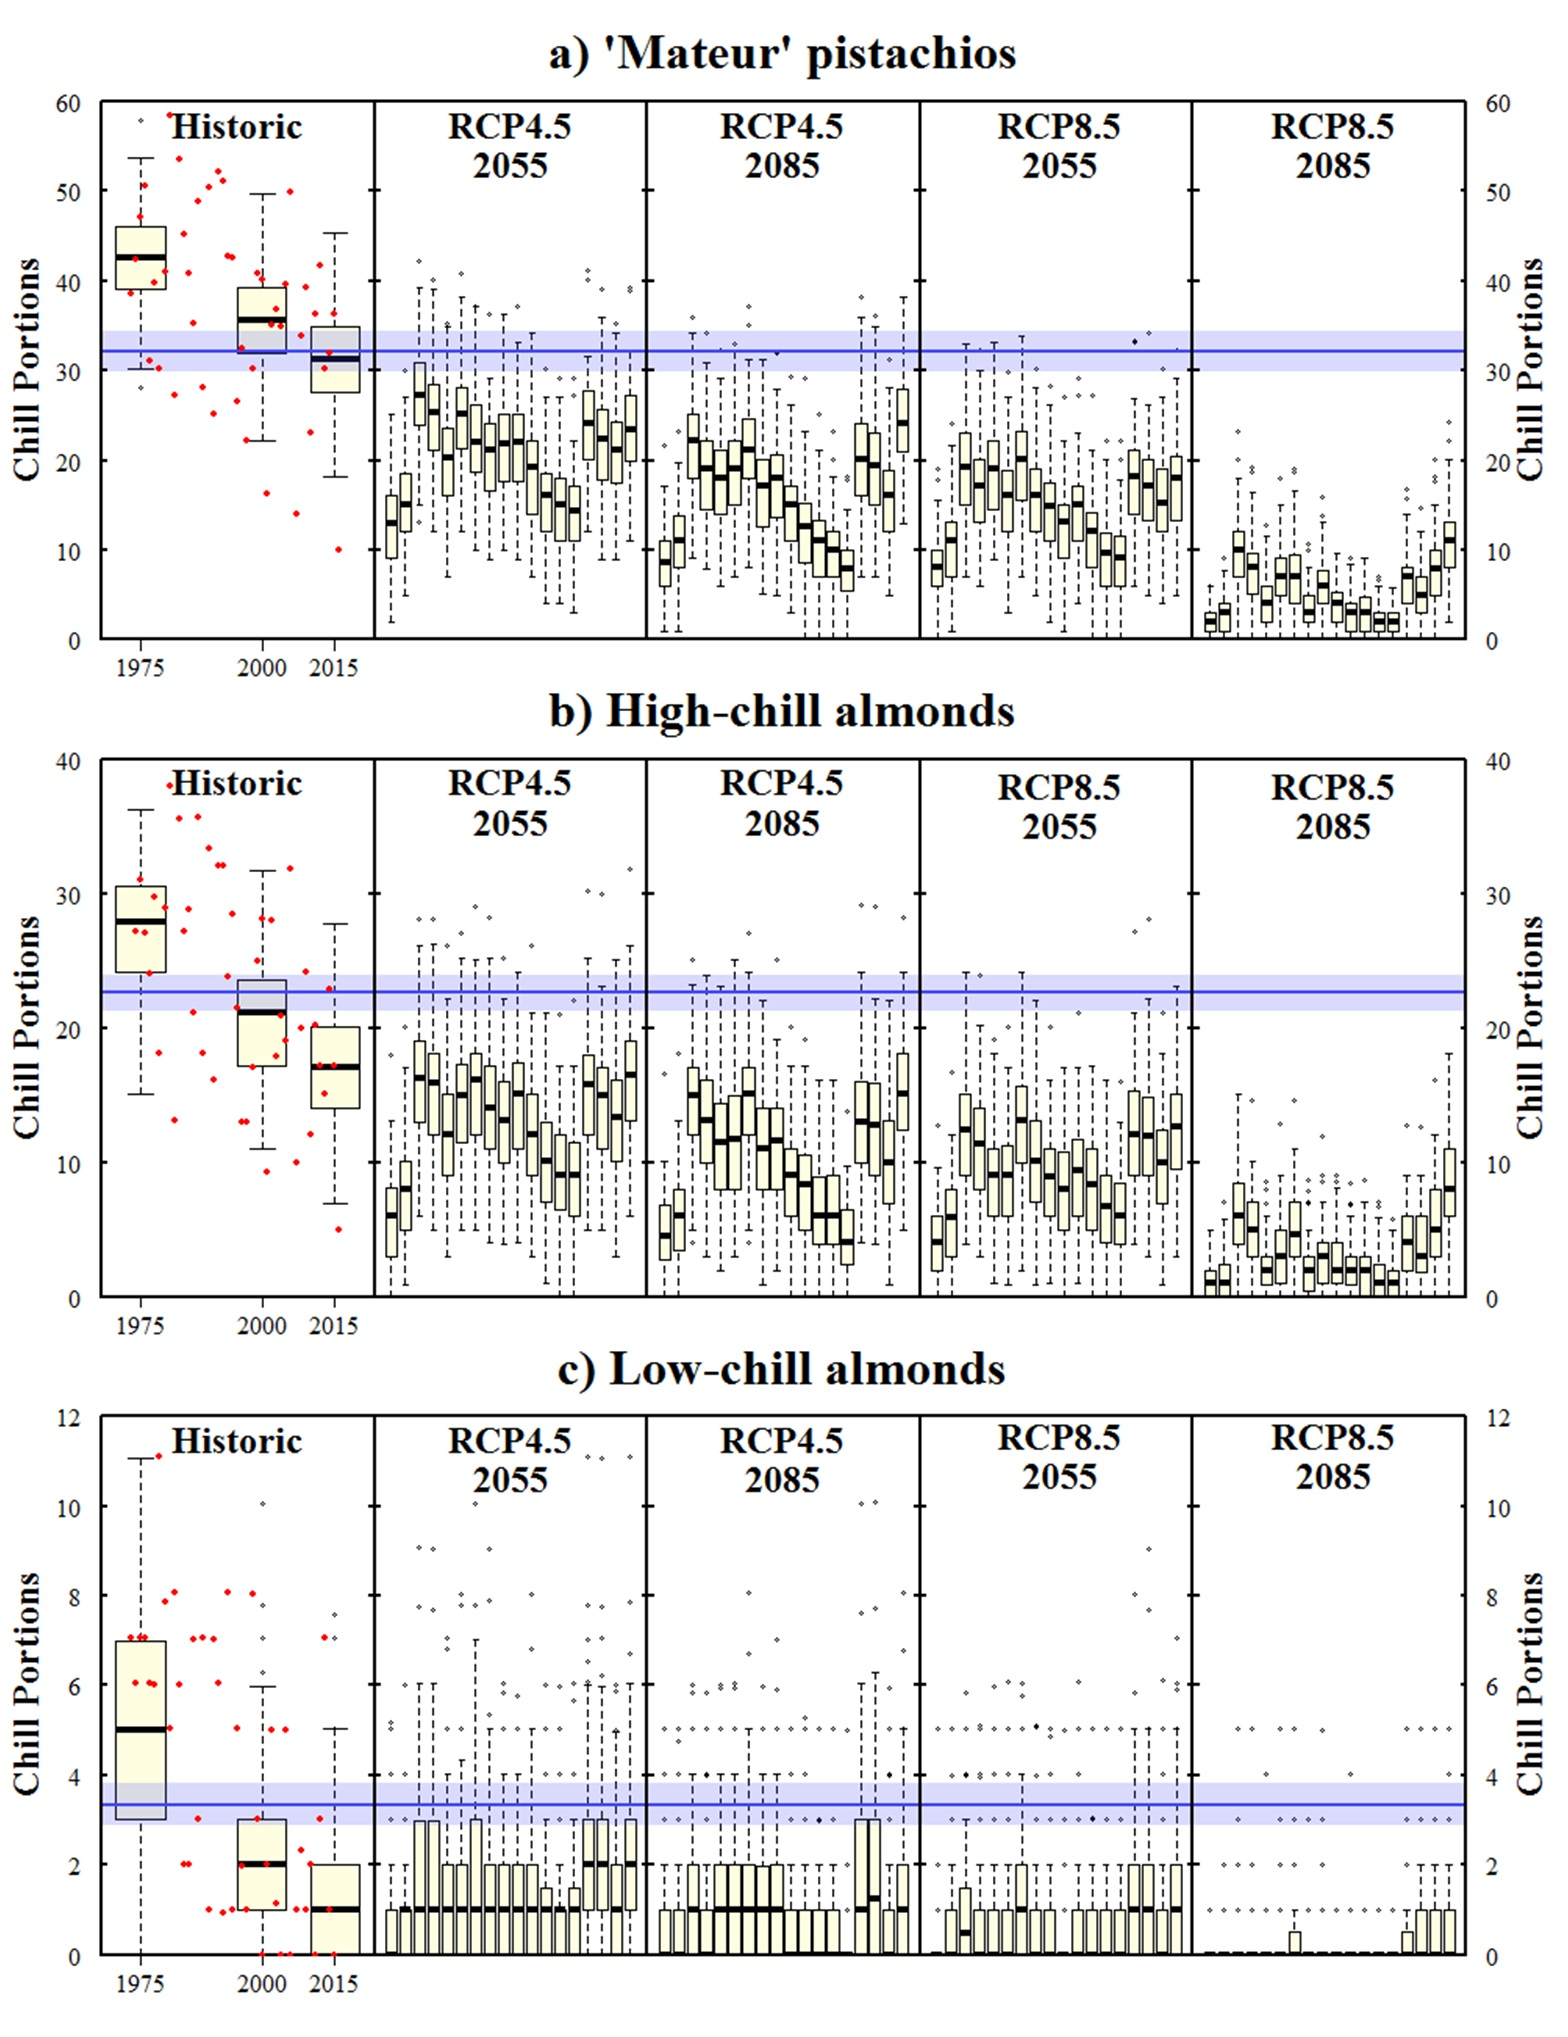
\includegraphics[width=0.9\textwidth,height=\textheight]{pictures/Tunisia_2018_Fig_1.jpg}
\caption{Winter chill analysis for an orchard near Sfax in Central Tunisia. The blue bars indicate approximate chilling requirements of pistachios and two types of almonds}
\end{figure}

If all goes well, you'll be able to produce such a figure by the end of the semester. This figure contains a number of interesting features that you'll learn about in this module. The plots on the left indicate the historic development of chill accumulation at this location. In this, the actually observed values are indicated by red dots. In addition to these dots, the plots also contain boxplots that describe the typical chill distribution at a particular point in time. These were generated with a weather generator that is accessed by \texttt{chillR}. This weather generator is calibrated with observed weather data and provided with an estimate of how various climate metrics differed from the long-term average climate in 1975, 2000 and 2015. With this information, we can generate a large number of artificial yearly weather records that might have occurred at these points in time.

The weather generator was also used to produce future scenarios. Also here, the tool was calibrated with observed weather data, but the scenarios that were added were not derived from the historic record, but extracted from the AFRICLIM database.

Now let's look at what this figure shows, because that it quite alarming. Usually, in a climate change projection, we would now start comparing forecasts for different scenarios, which are often not entirely consistent. Here, we don't have such a problem. It seems very clear that there is not a single future scenario in this analysis, where cultivation of pistachios or high-chill almonds remains viable! This conclusion is based on the assumption that our understanding of how to quantify winter chill isn't totally wrong. It is supported by recent observations in Tunisia, where, after the particularly warm winter of 2015/16, many pistachio trees barely developed any flowers, which resulted in virtually complete crop failure:

\begin{figure}
\centering
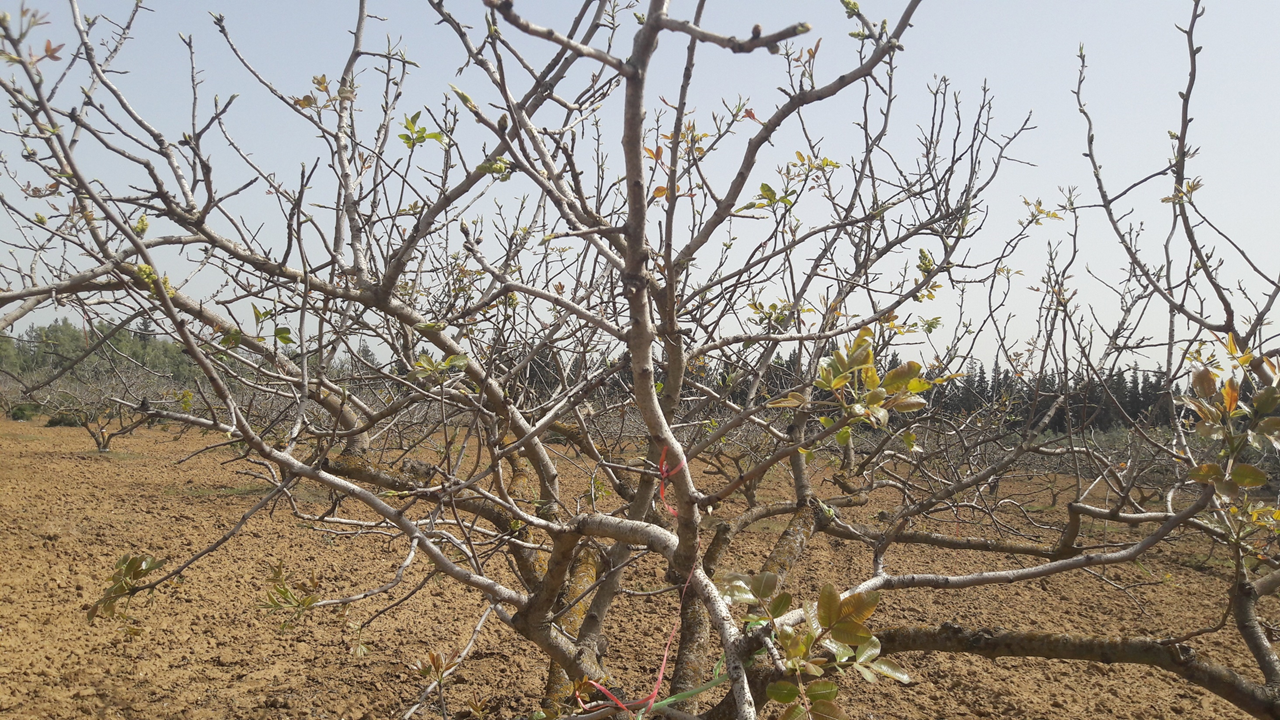
\includegraphics[width=0.9\textwidth,height=\textheight]{pictures/Tunisia_pistachios.png}
\caption{Pistachio tree near Sfax, Central Tunisia, in April of 2016, after a particularly warm winter. This tree clearly didn't fulfill its chilling requirement}
\end{figure}

\hypertarget{winter-chill-in-chile}{%
\subsection{Winter chill in Chile}\label{winter-chill-in-chile}}

AFRICLIM solved the future climate data problem for locations in Africa. However, this dataset fell short of what was needed in order to add climate change projection capability to \texttt{chillR}. First, it was unsatisfying that this dataset only covered Africa. Second, users who are only interested in data for a single location, which is what \texttt{chillR} is designed for, shouldn't have to download a large dataset, before they can run analyses. What was needed was a tool that could quickly access single-location data for weather stations anywhere on the planet.

One of my early sources of climate information was a tool called `ClimateWizard', put together by my friend and collaborator \href{https://scholar.google.de/citations?user=Yh2sQY4AAAAJ\&hl=de}{Evan Girvetz}, who now works for the International Centre for Tropical Agriculture (CIAT) in Nairobi. This tool initially only made gridded data available, but already for the California study cited above \href{https://journals.plos.org/plosone/article?id=10.1371/journal.pone.0006166}{(Luedeling, Zhang, and Girvetz \protect\hyperlink{ref-luedeling_climatic_2009}{2009})}, Evan had written a script to quickly extract information for single locations, which is really all that's needed for single-site studies. Eventually, at CIAT, he made this function available to a wider audience through an application programming interface (API), to allow accessing outputs from 15 climate models for state-of-the-art RCP scenarios.

This tool allowed us, in this case led by \href{https://scholar.google.de/citations?hl=de\&user=ibSma_AAAAAJ}{Eduardo Fernández}, to expand our geographic reach into South America. Focusing on nine locations throughout Chile, Eduardo analyzed past and future chill development across a wide climatic gradient \href{https://link.springer.com/article/10.1007/s10584-019-02608-1}{(Fernandez et al. \protect\hyperlink{ref-fernandez2020prospects}{2020})}.

\begin{figure}
\centering
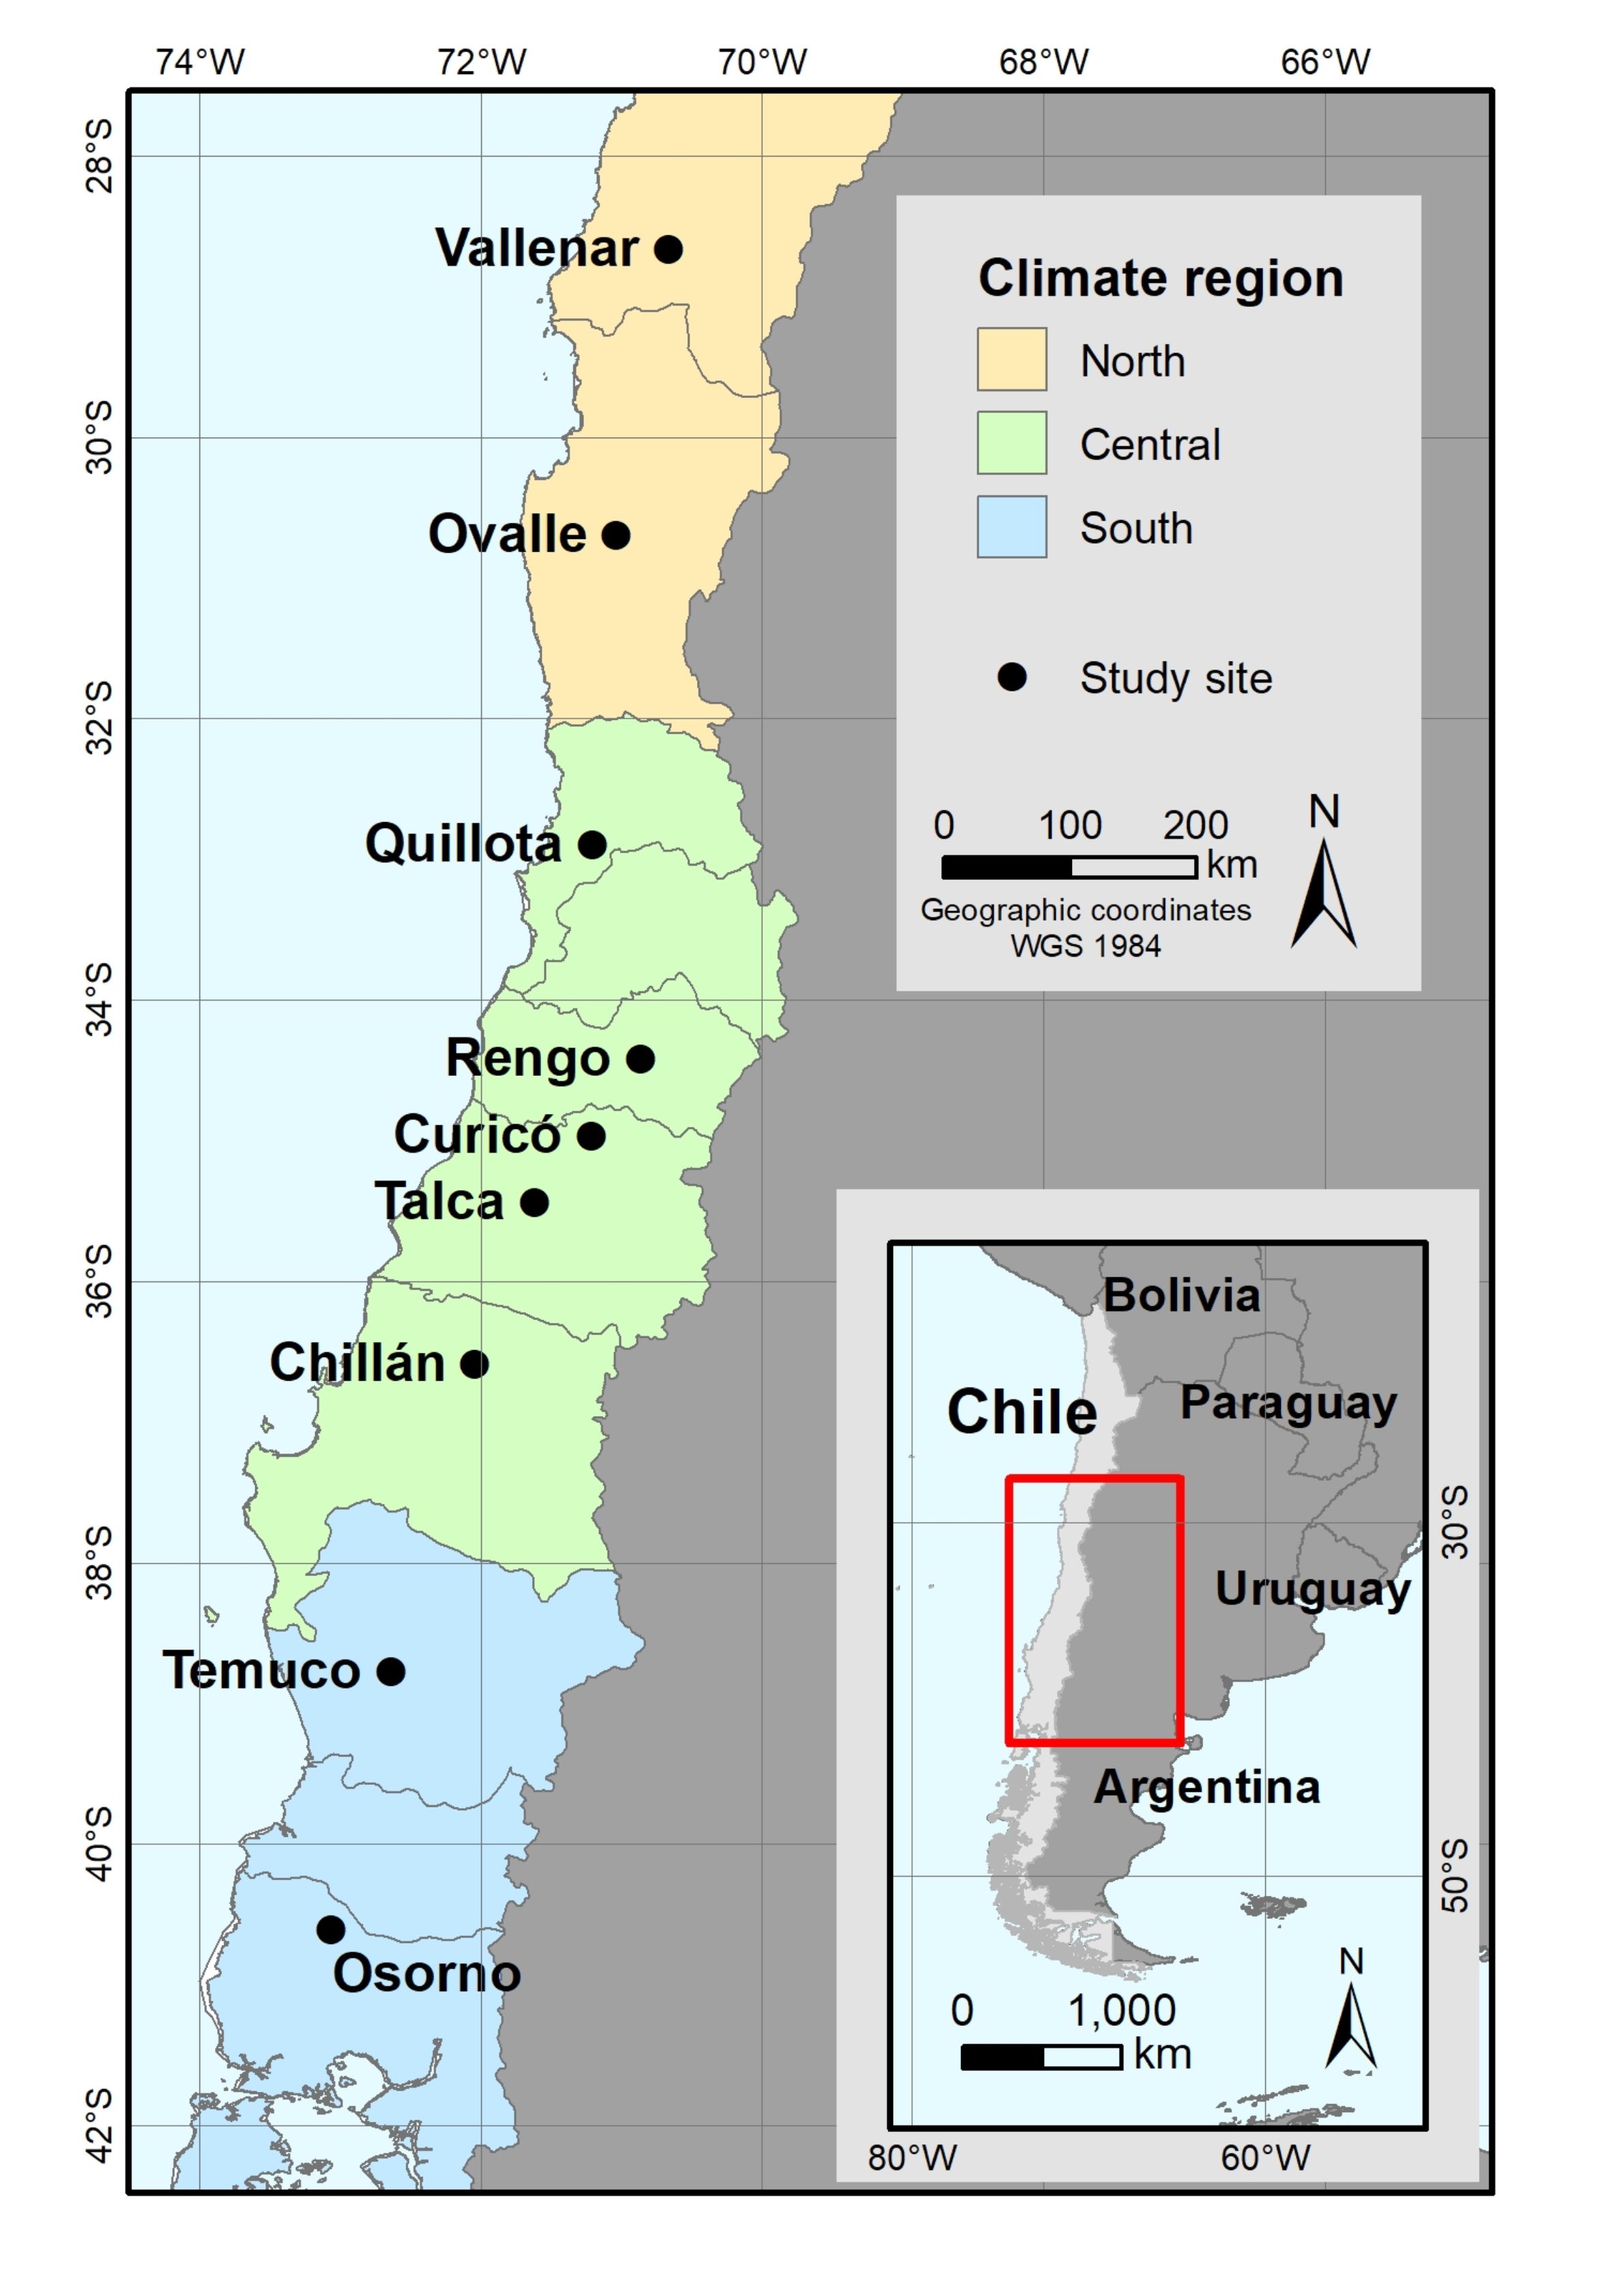
\includegraphics[width=0.9\textwidth,height=\textheight]{pictures/Chile_chill_map.png}
\caption{Map of fruit growing locations in Chile, for which chill accumulation was assessed}
\end{figure}

\begin{figure}
\centering
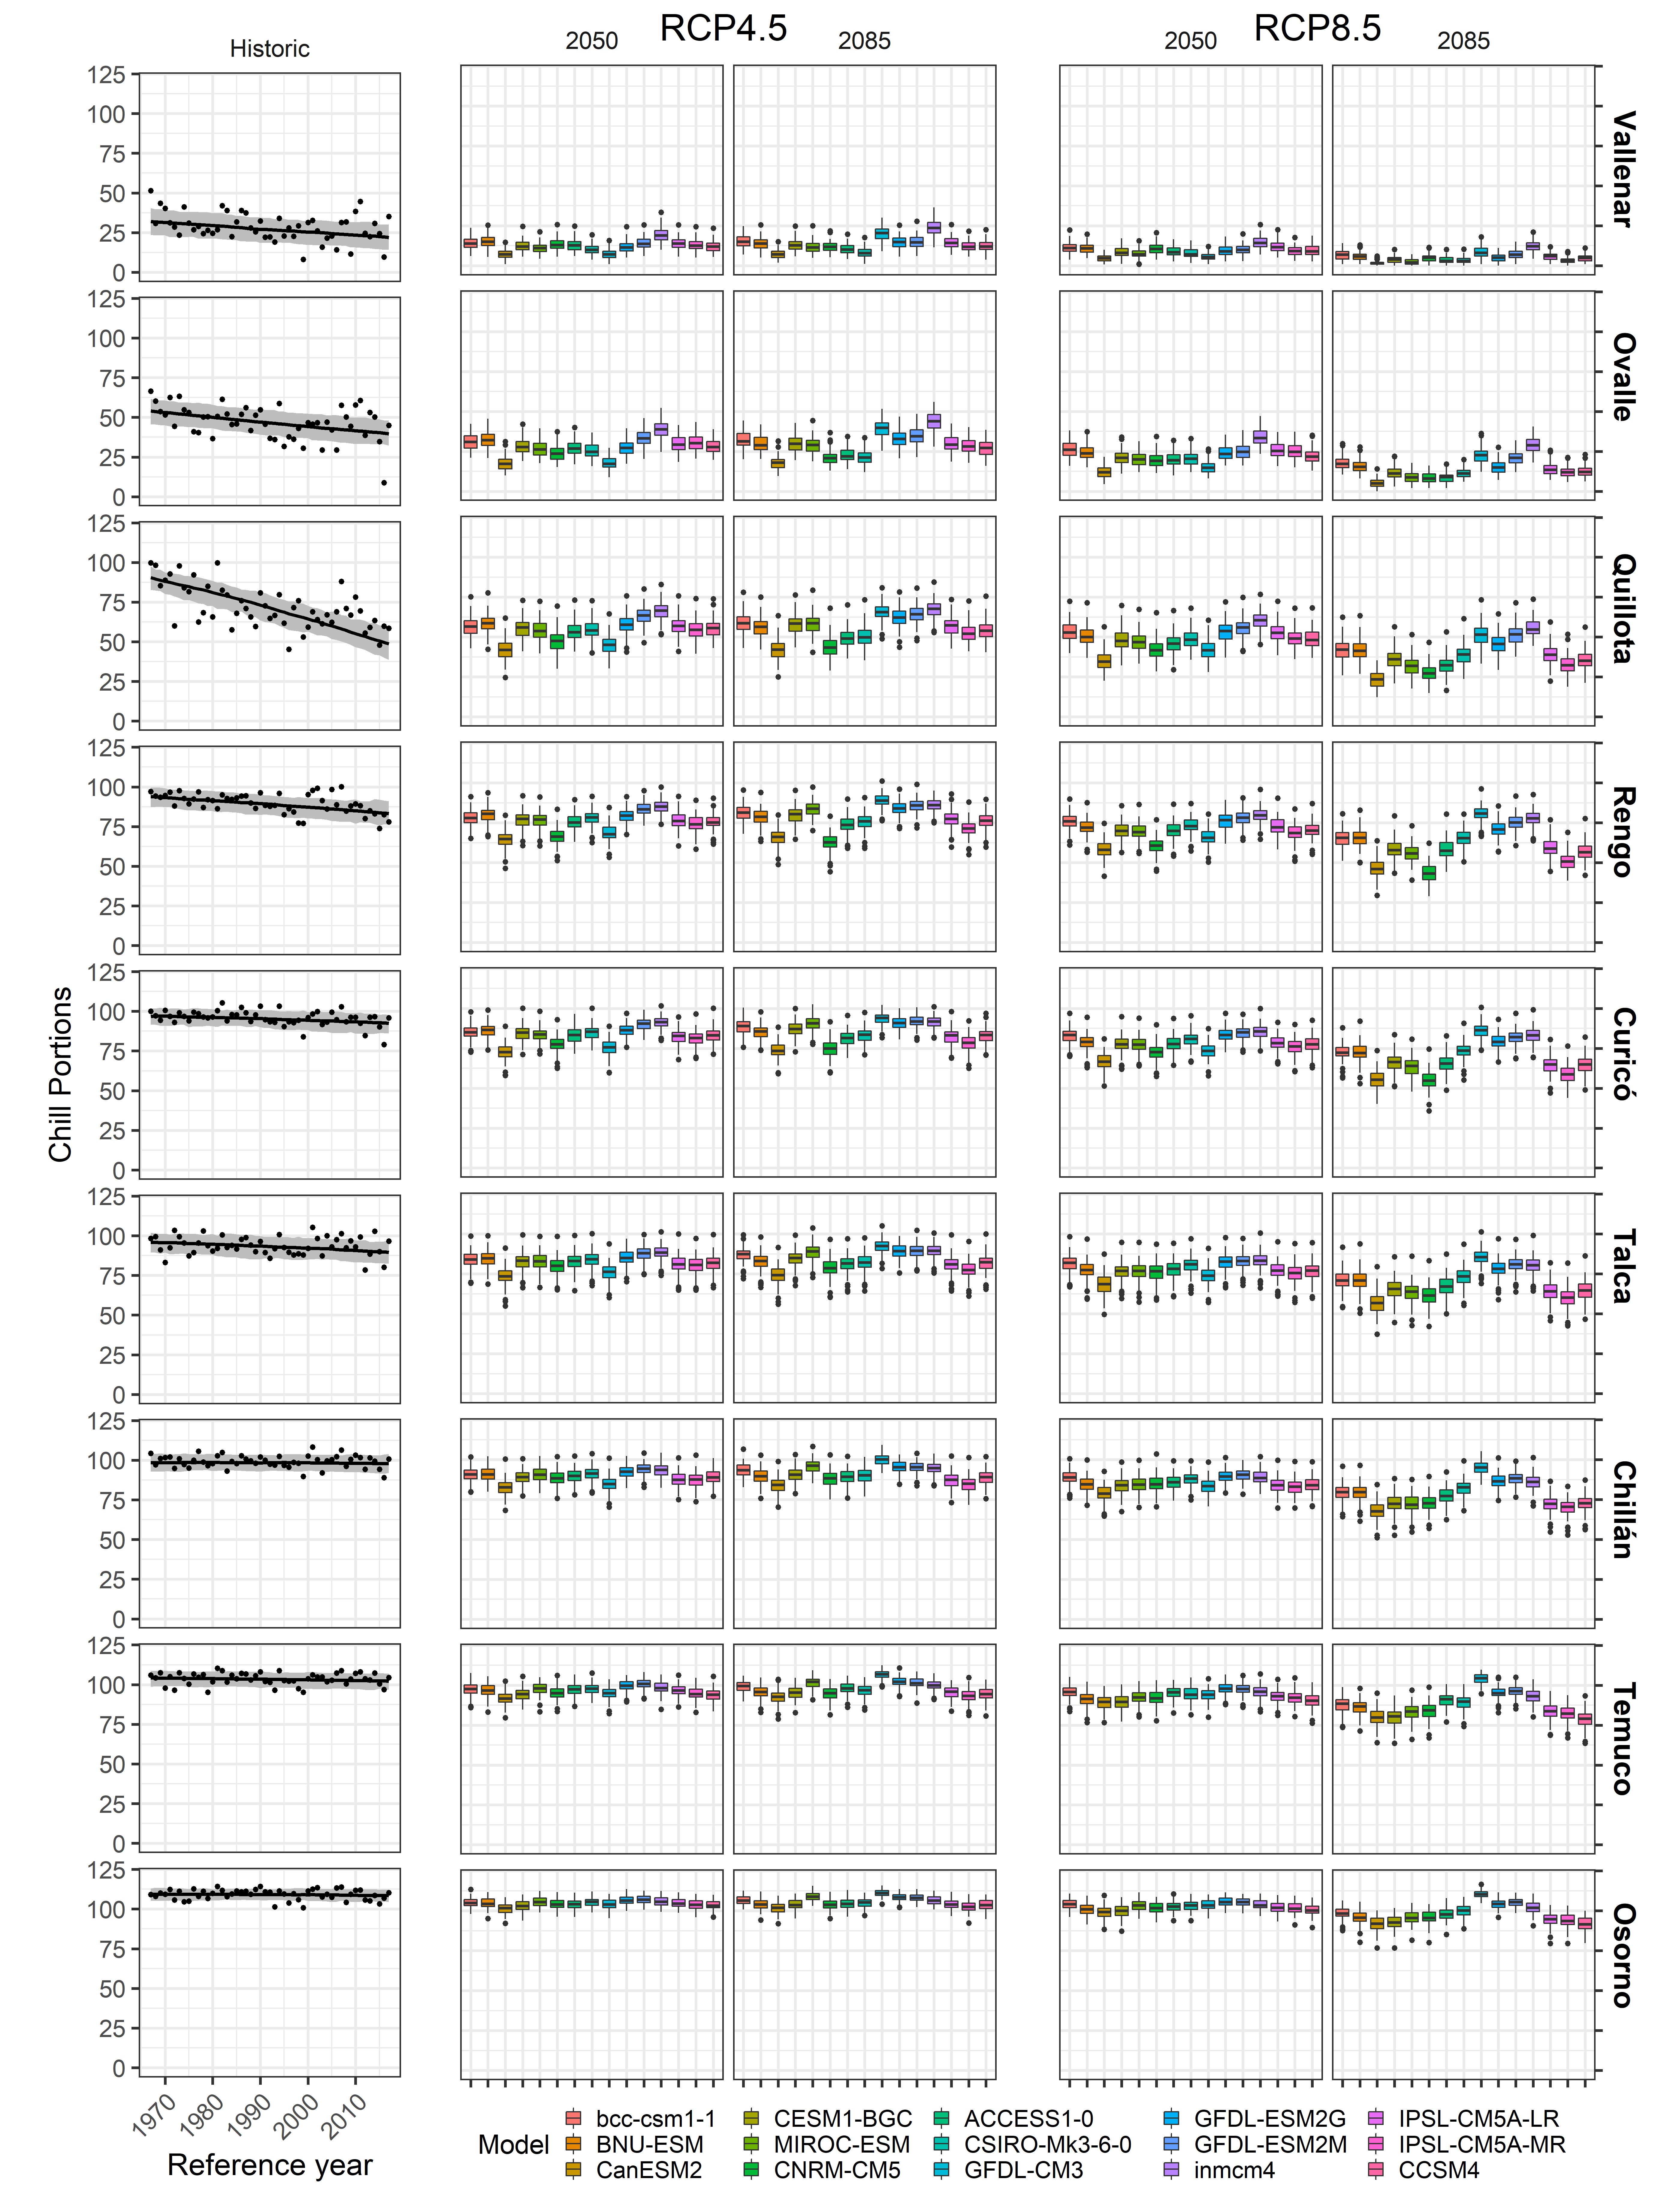
\includegraphics[width=0.9\textwidth,height=\textheight]{pictures/Chile_chill_all.png}
\caption{Assessment of past and future winter chill for 9 locations across Chile}
\end{figure}

Apparently, Eduardo didn't like my plot design, so he redesigned it using the \texttt{ggplot2} package, a powerful plotting package for R. One of the things that we can see here is that with data for many sites, things get a bit too complex to easily grasp. So Eduardo thought of a creative way to extract some key information for each scenario and display it as a heat map:

\begin{figure}
\centering
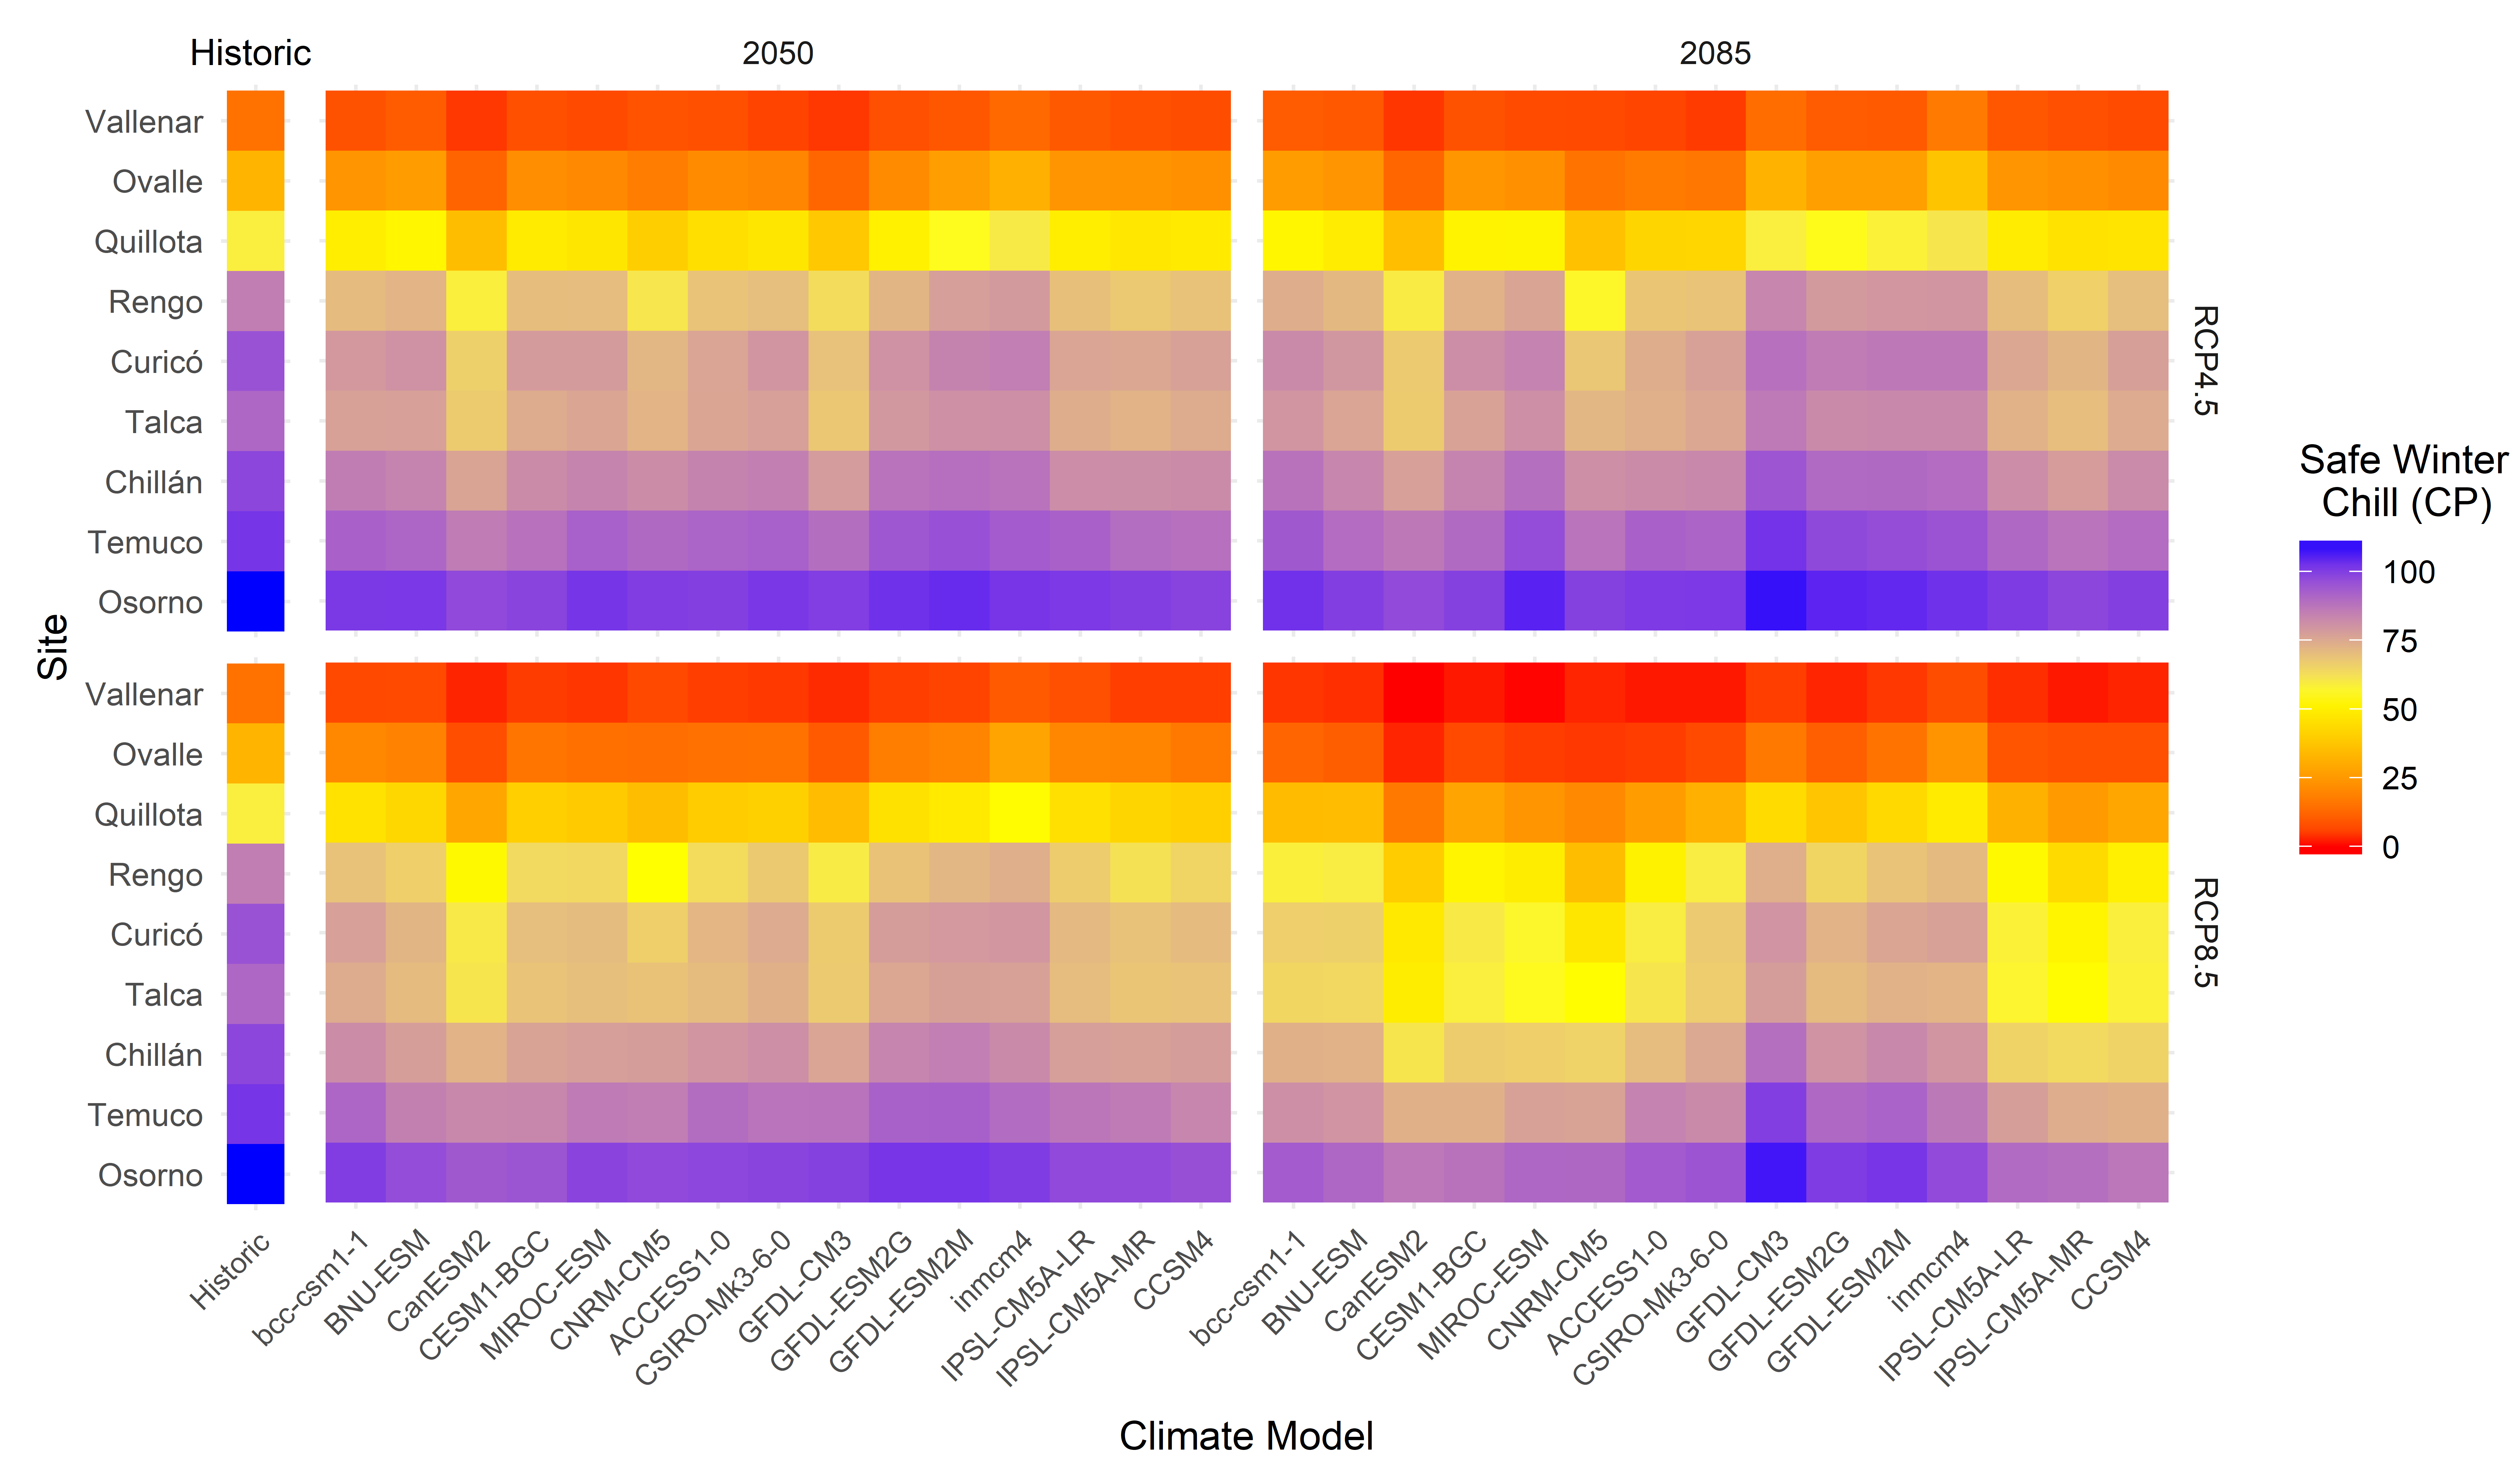
\includegraphics[width=0.9\textwidth,height=\textheight]{pictures/Chile_chill_heatmap.png}
\caption{Heatmap showing Safe Winter Chill (10\% quantile of chill distribution) for nine locations in Chile}
\end{figure}

We see here clearly the north-south gradient in available chill, as well as (less clearly) the tendency for lower chill towards the right panels, especially towards the lower right corner.

\hypertarget{chill-projection-for-patagonia}{%
\subsection{Chill projection for Patagonia}\label{chill-projection-for-patagonia}}

Some locations on our planet may become more hospitable for agriculture, as the climate changes. We used our analysis framework to look into the climatic suitability for fruit and nut trees near agriculture's southern frontier - in Patagonia, in southern Argentina \href{https://rmets.onlinelibrary.wiley.com/doi/pdf/10.1002/joc.6649}{(del Barrio et al. \protect\hyperlink{ref-delclimate}{2020})}.

\begin{figure}
\centering
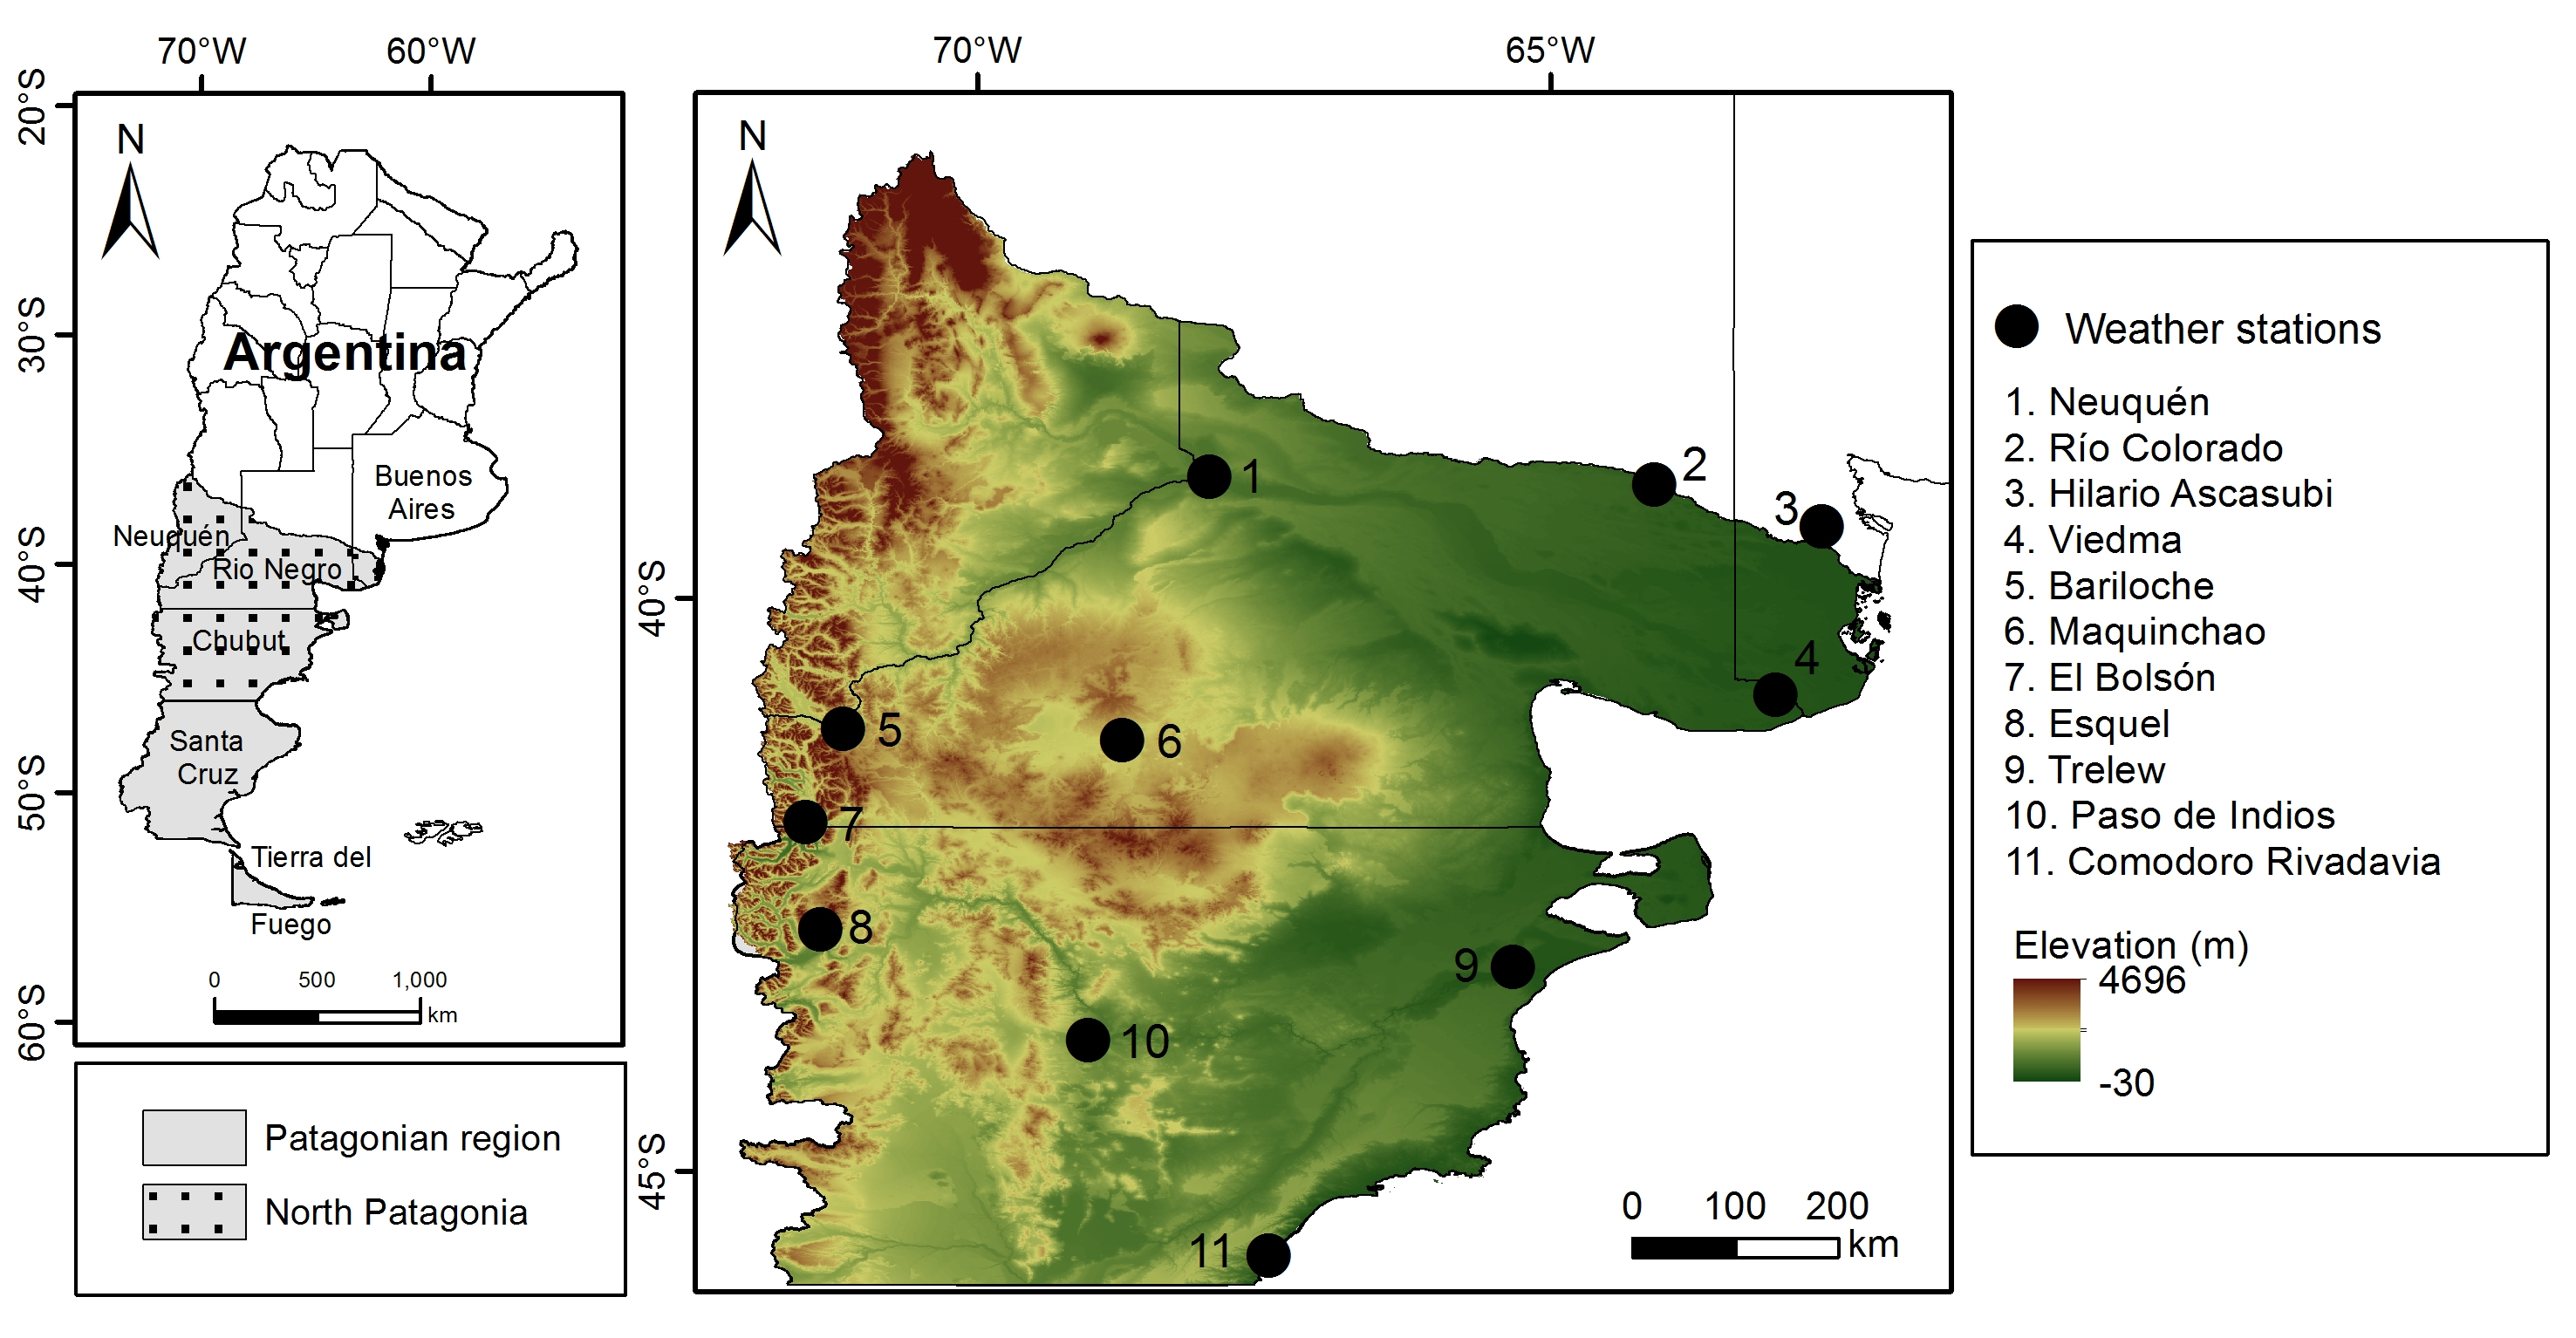
\includegraphics[width=0.9\textwidth,height=\textheight]{pictures/Patagonia_map.png}
\caption{Map of parts of Patagonia in Argentina, showing locations that were analyzed in this study}
\end{figure}

We got weather station records for all the locations shown in the map, used them to calibrate our weather generator and downloaded climate projections from the ClimateWizard database. This then allowed making past and future temperature scenarios for all stations and to compute winter chill and a few other agroclimatic metrics.

Results of the winter chill calculation were not so interesting here, with very little change projected.

\begin{figure}
\centering
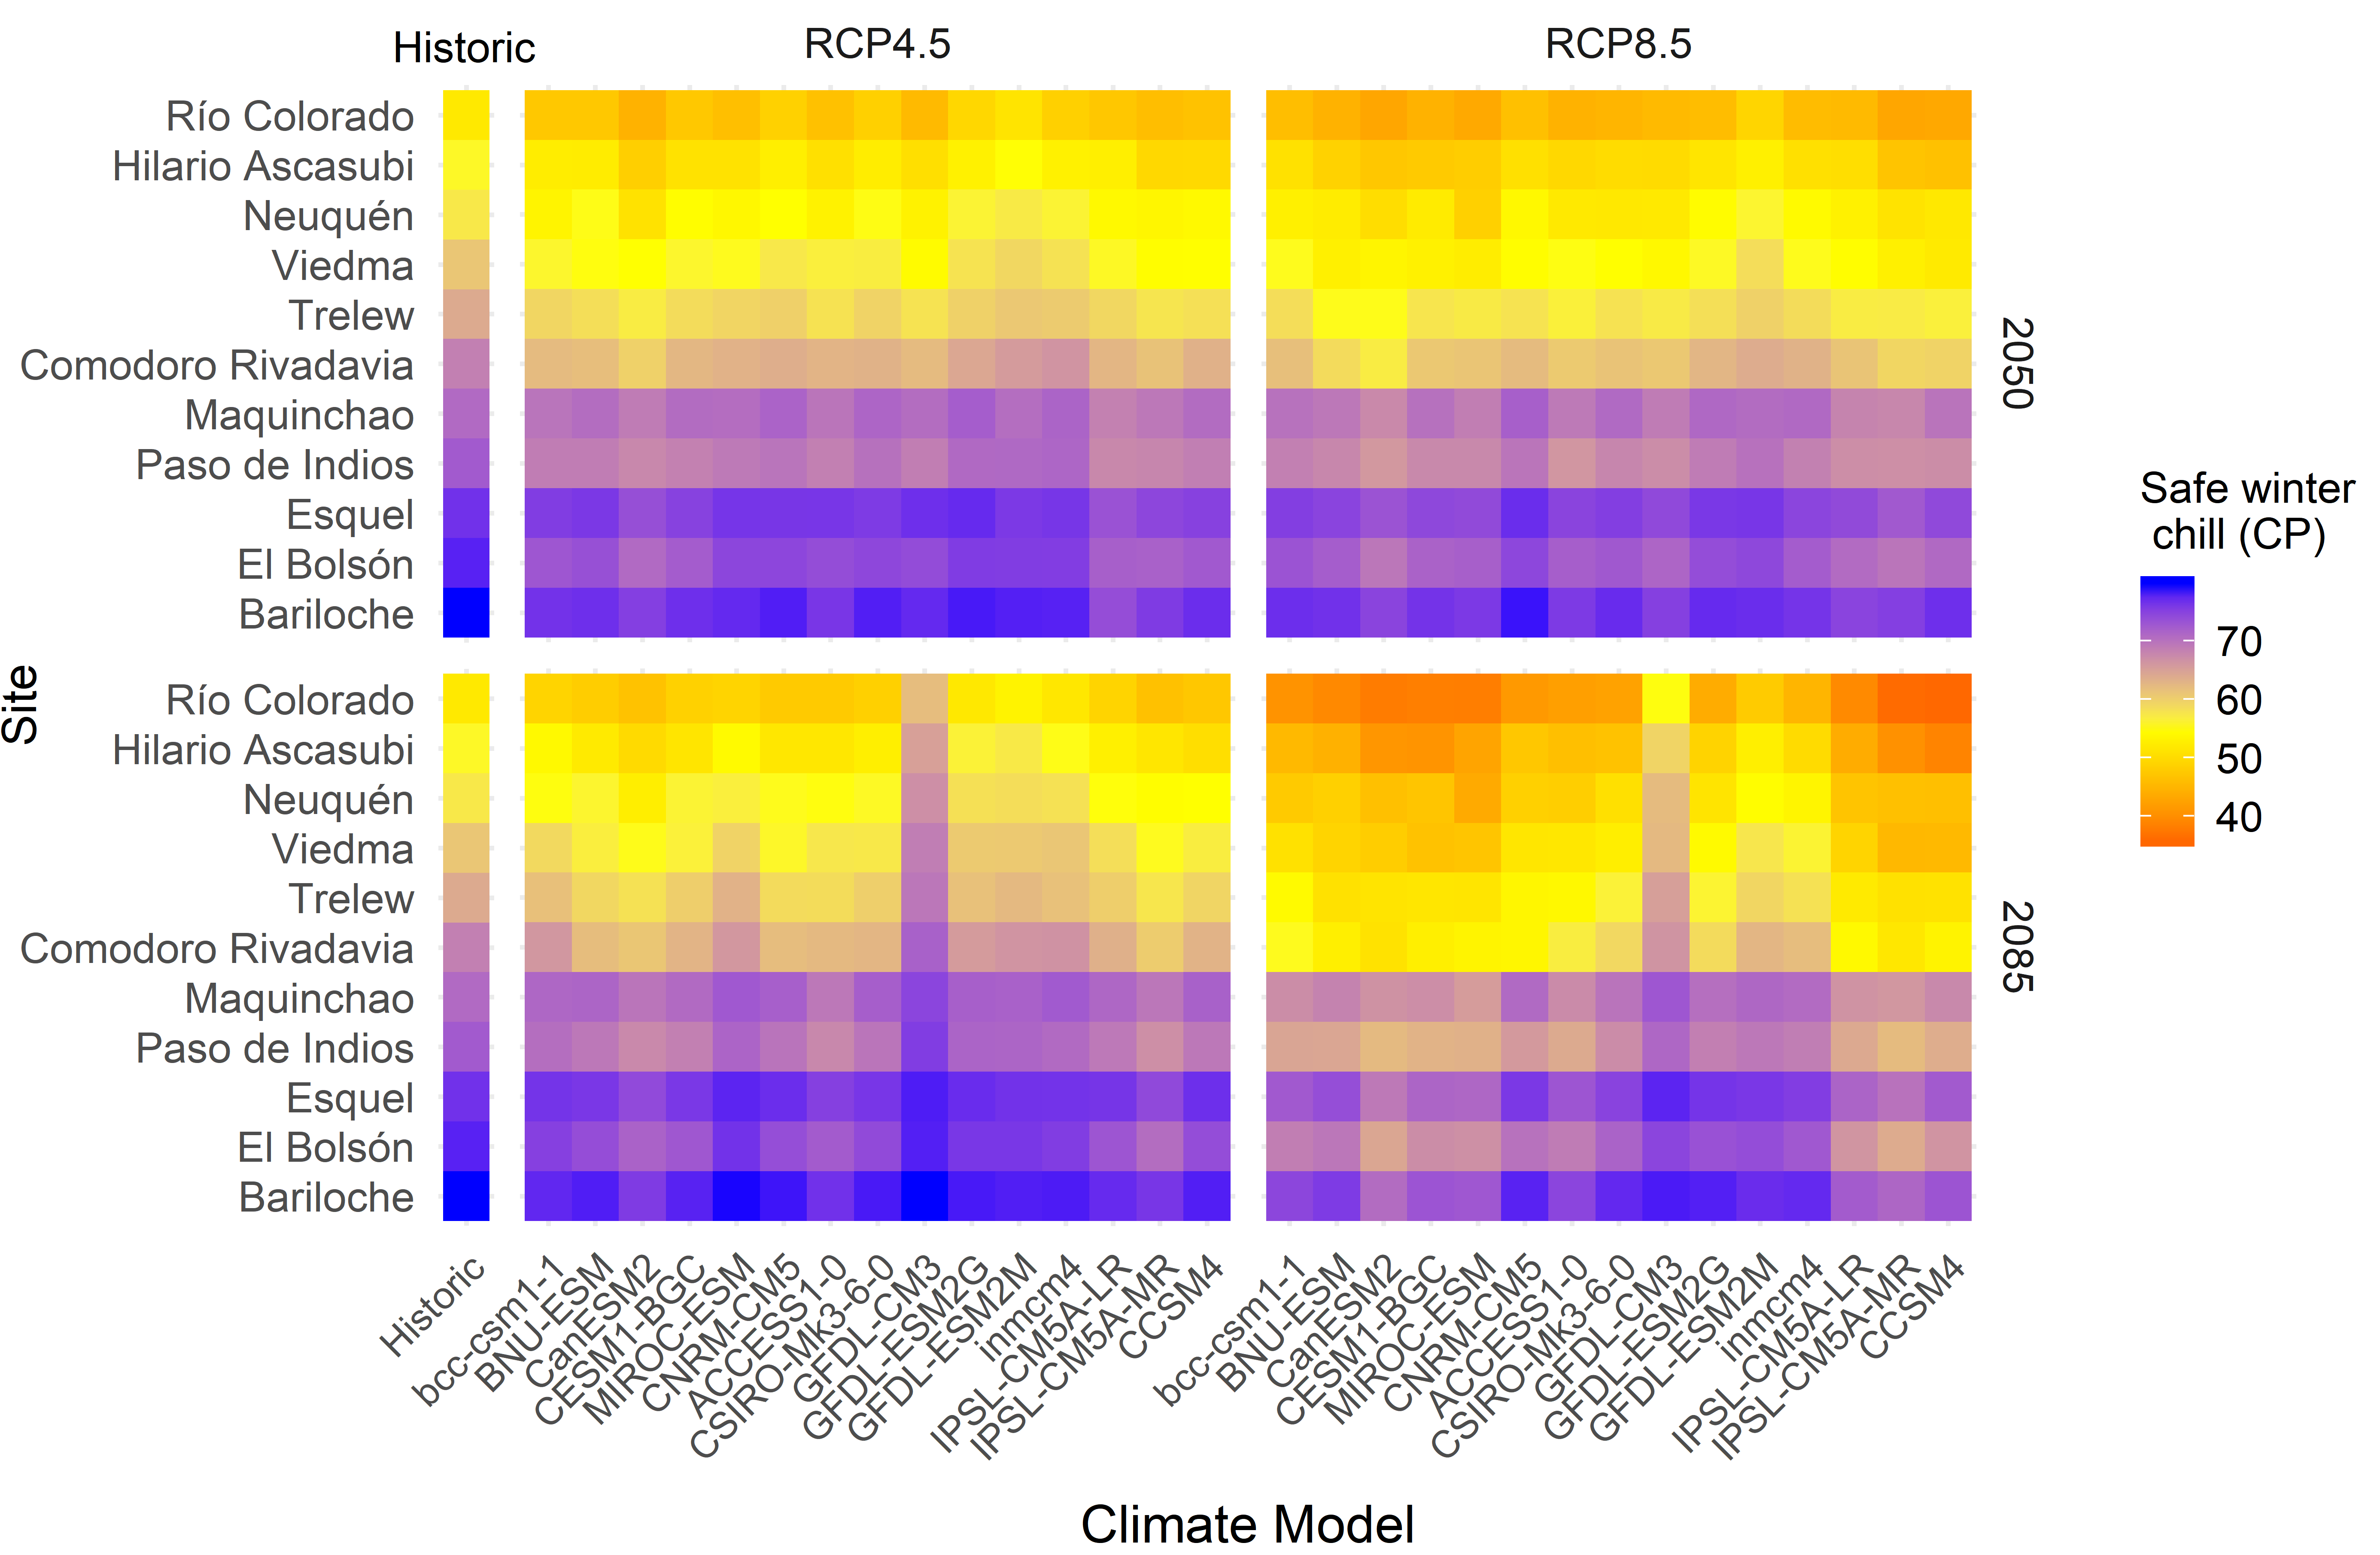
\includegraphics[width=0.9\textwidth,height=\textheight]{pictures/Patagonia_heatmap.png}
\caption{Heatmap showing Safe Winter Chill (10\% quantile of chill distribution) for eleven locations in Patagonia}
\end{figure}

In fact, climate change may have a positive effect on land suitability for fruit trees, because more summer heat will be available:

\begin{figure}
\centering
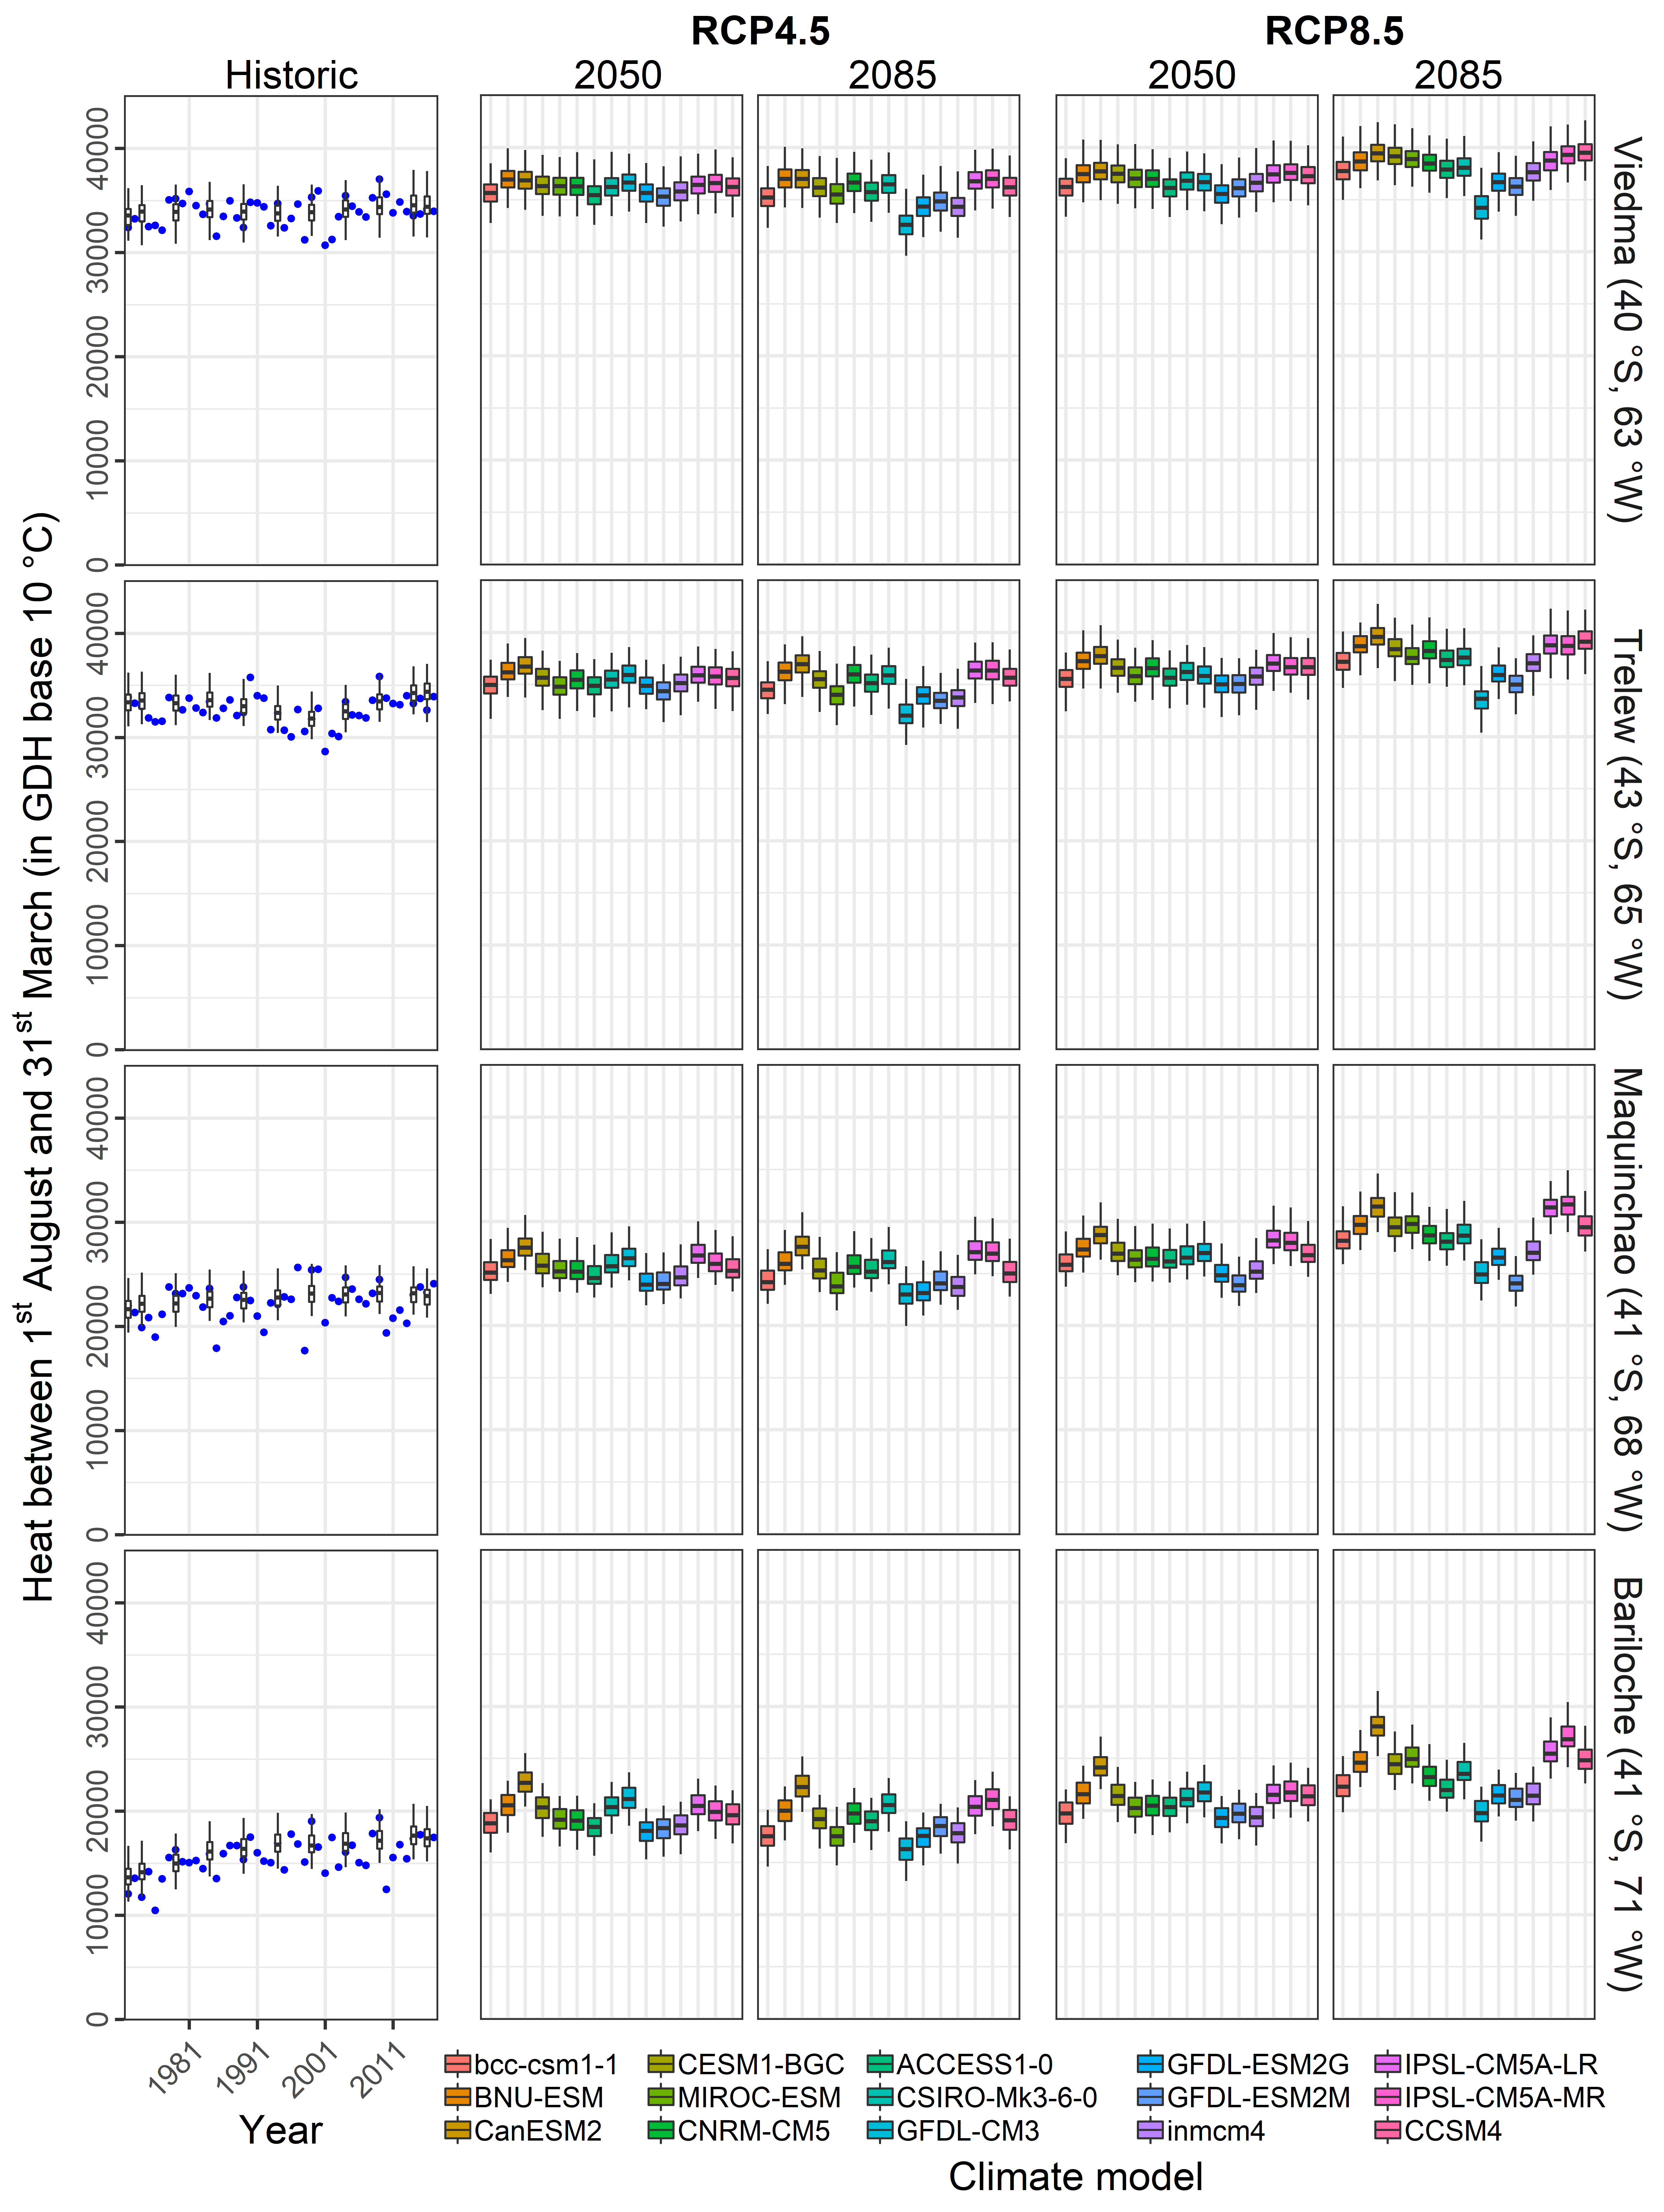
\includegraphics[width=0.9\textwidth,height=\textheight]{pictures/Patagonia_heat.png}
\caption{Past and projected future heat availability for three exemplary locations in Patagonia}
\end{figure}

A further beneficial development is a likely reduction in the number of frost hours:

\begin{figure}
\centering
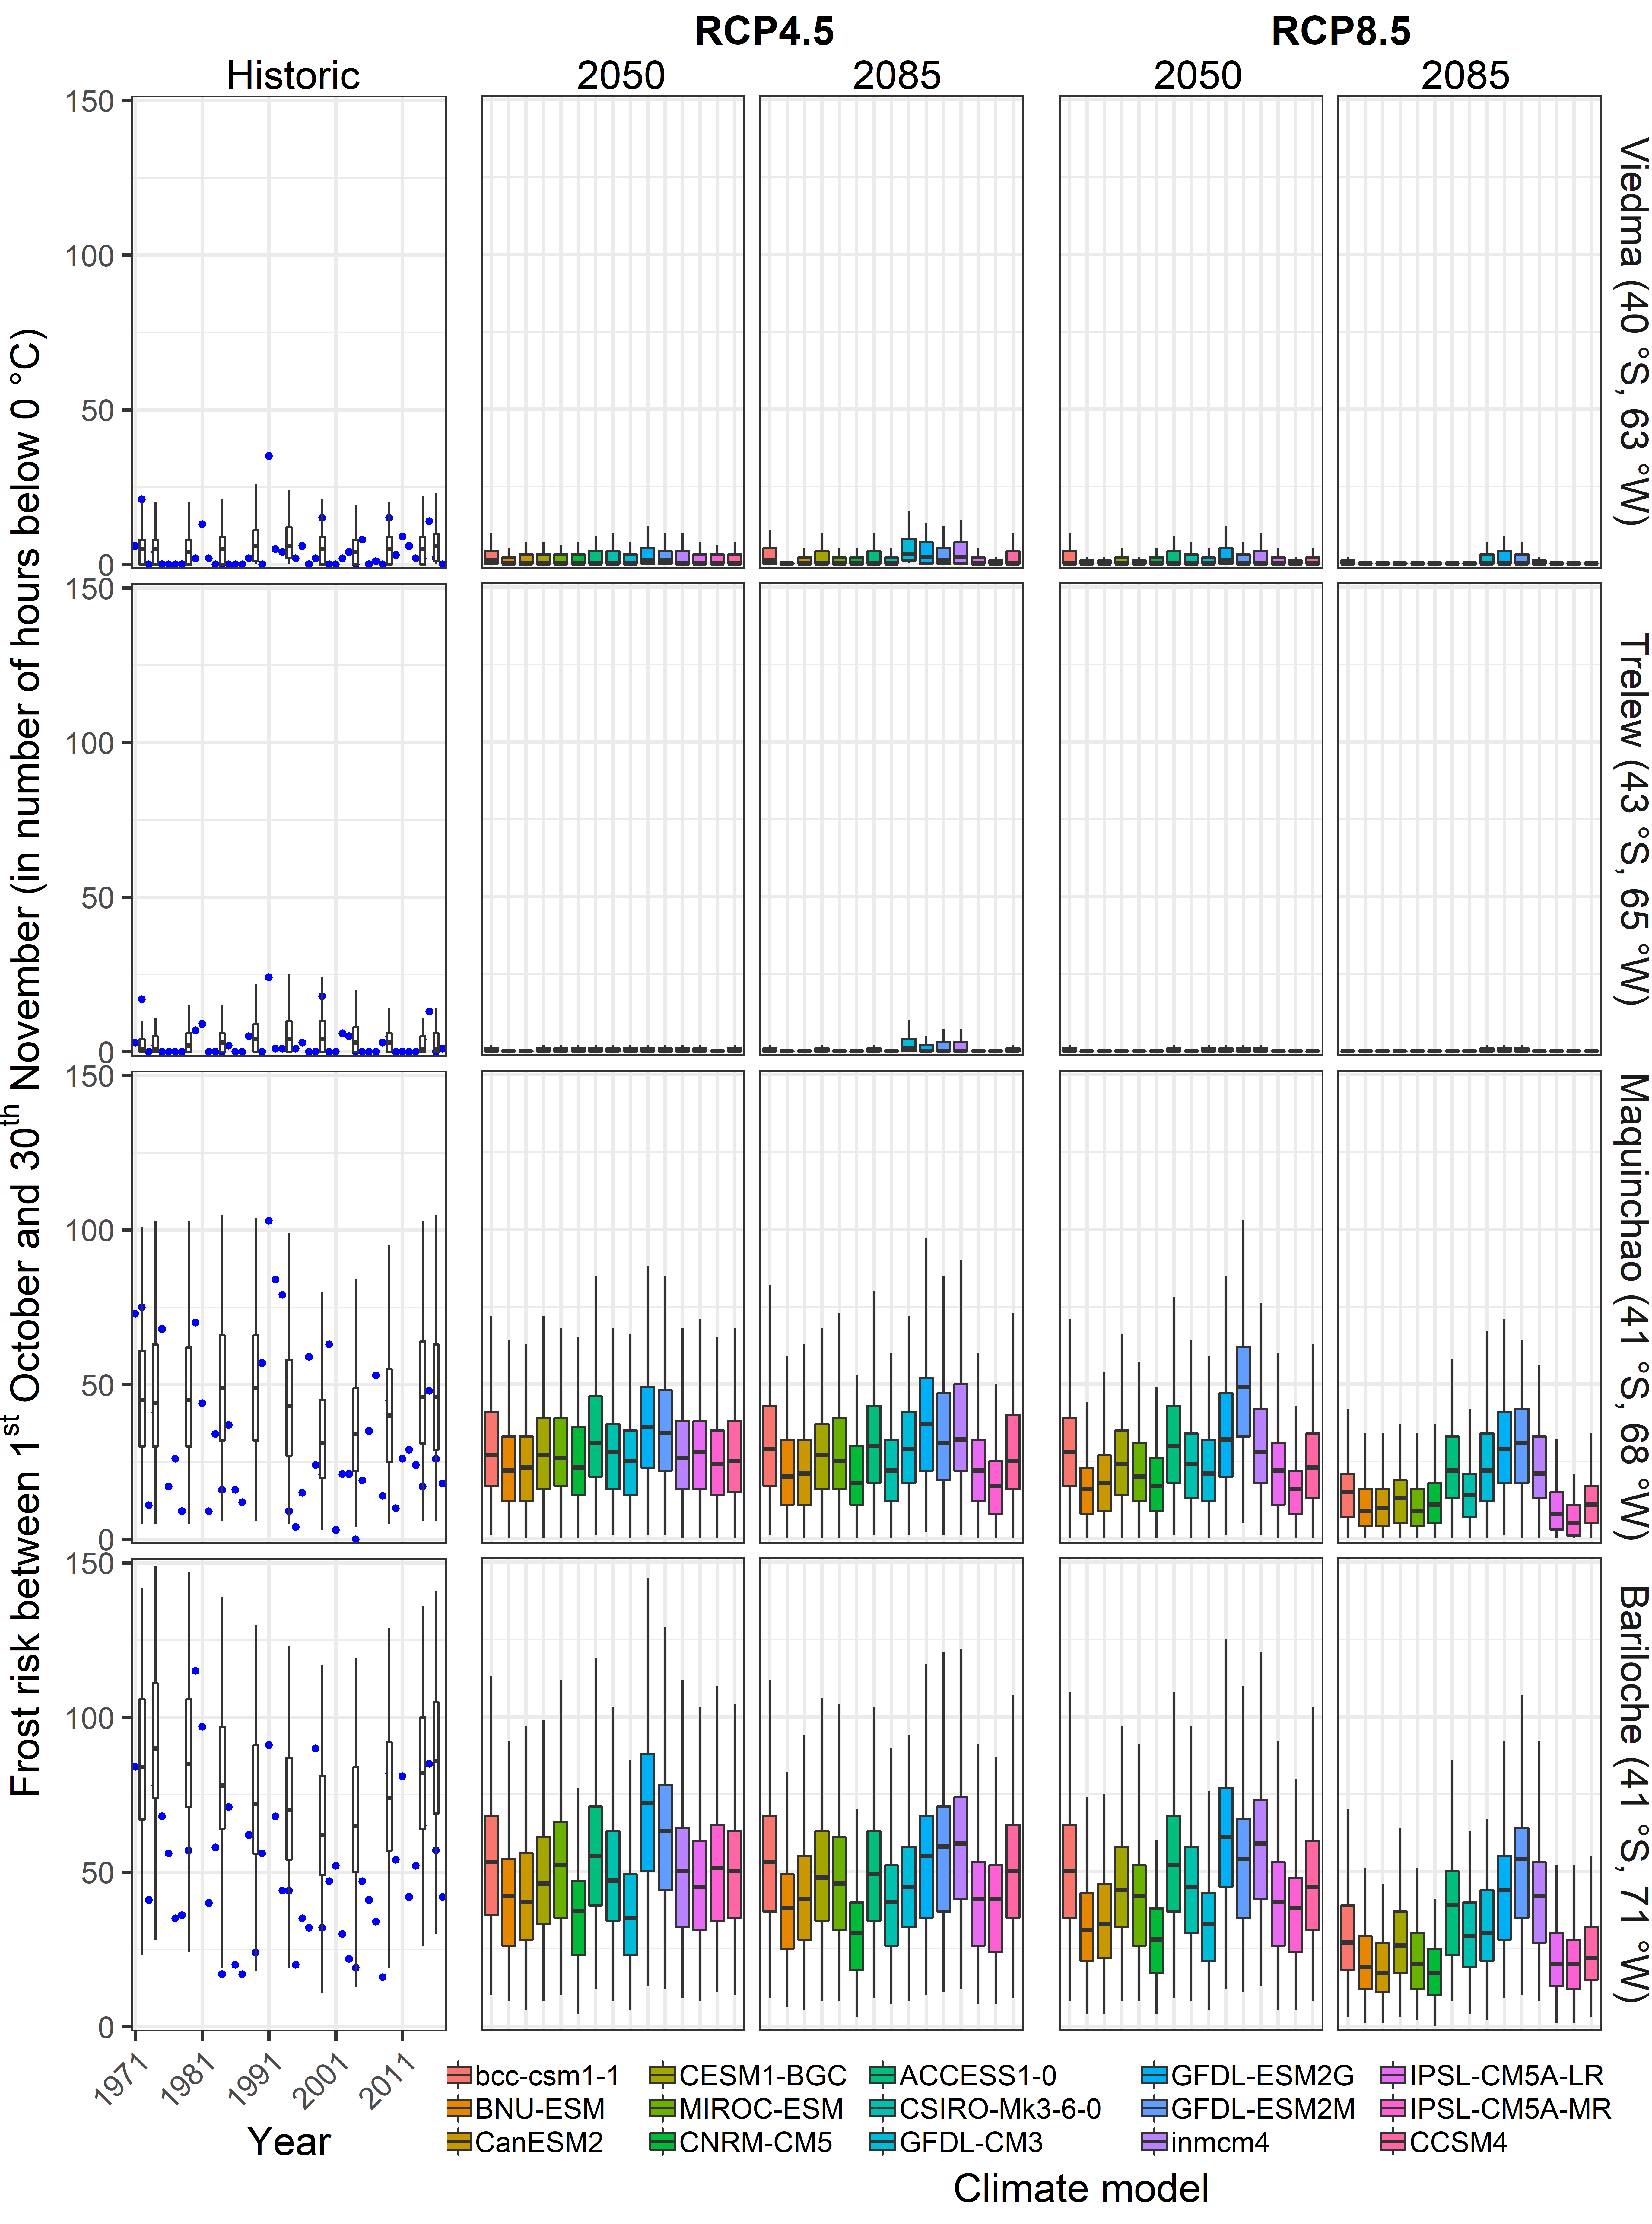
\includegraphics[width=0.9\textwidth,height=\textheight]{pictures/Patagonia_frost.png}
\caption{Past and projected frost risk for three exemplary locations in Patagonia}
\end{figure}

This may all not look very spectacular, but it seems quite likely to me that the small changes we're seeing will promote many locations from a climate that is really too cool for agriculture, especially for fruit trees, to a fairly optimal situation. For a change, some possibly good news related to climate change (though also this will likely come with negative implications for natural ecosystems and possibly other agricultural systems).

\hypertarget{chill-model-comparison}{%
\subsection{Chill model comparison}\label{chill-model-comparison}}

Eduardo Fernandez recently used our climate change analysis framework to compare chill models \href{https://www.sciencedirect.com/science/article/abs/pii/S1161030120301106}{(Fernandez, Whitney, and Luedeling \protect\hyperlink{ref-fernandez2020importance}{2020})}, greatly expanding on my earlier chill model comparisons (Luedeling and Brown \protect\hyperlink{ref-luedeling_global_2011}{2011}). He assembled a collection of 13 approaches to quantify chill accumulation from the literature and applied the models he found to datasets from a number of locations in Germany, Tunisia and Chile (the countries involed in our \href{https://pasitproject.de/}{PASIT} project). Here's a map of the locations:

\begin{figure}
\centering
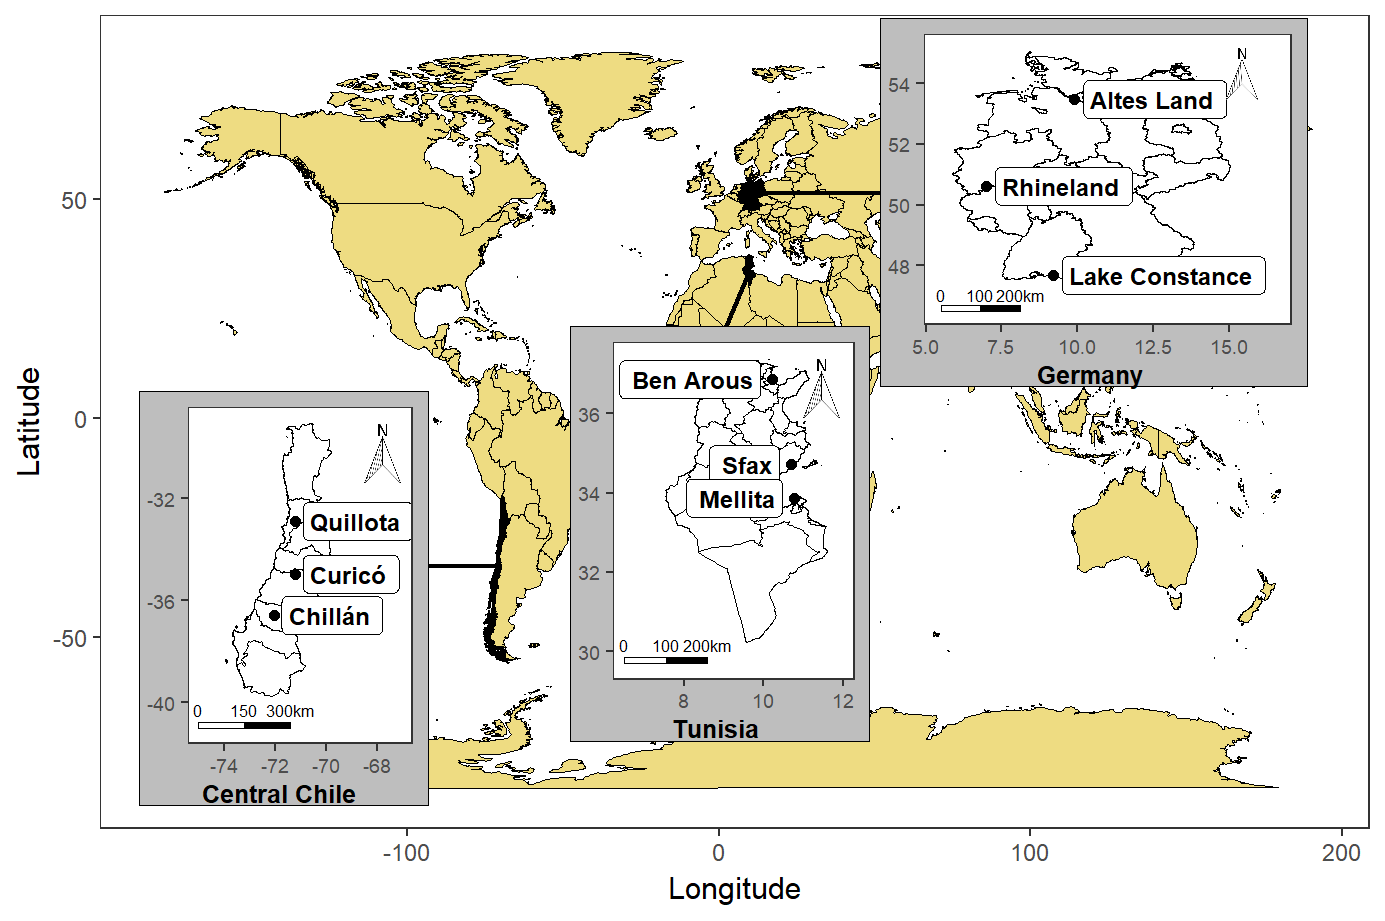
\includegraphics[width=0.9\textwidth,height=\textheight]{pictures/Model_comp_map.png}
\caption{Locations used for comparing predictions by a total of 13 chill models across different climates}
\end{figure}

The expectation was that the models would differ strongly in the extent of changes they predicted. This expectation was not disappointed:

\begin{figure}
\centering
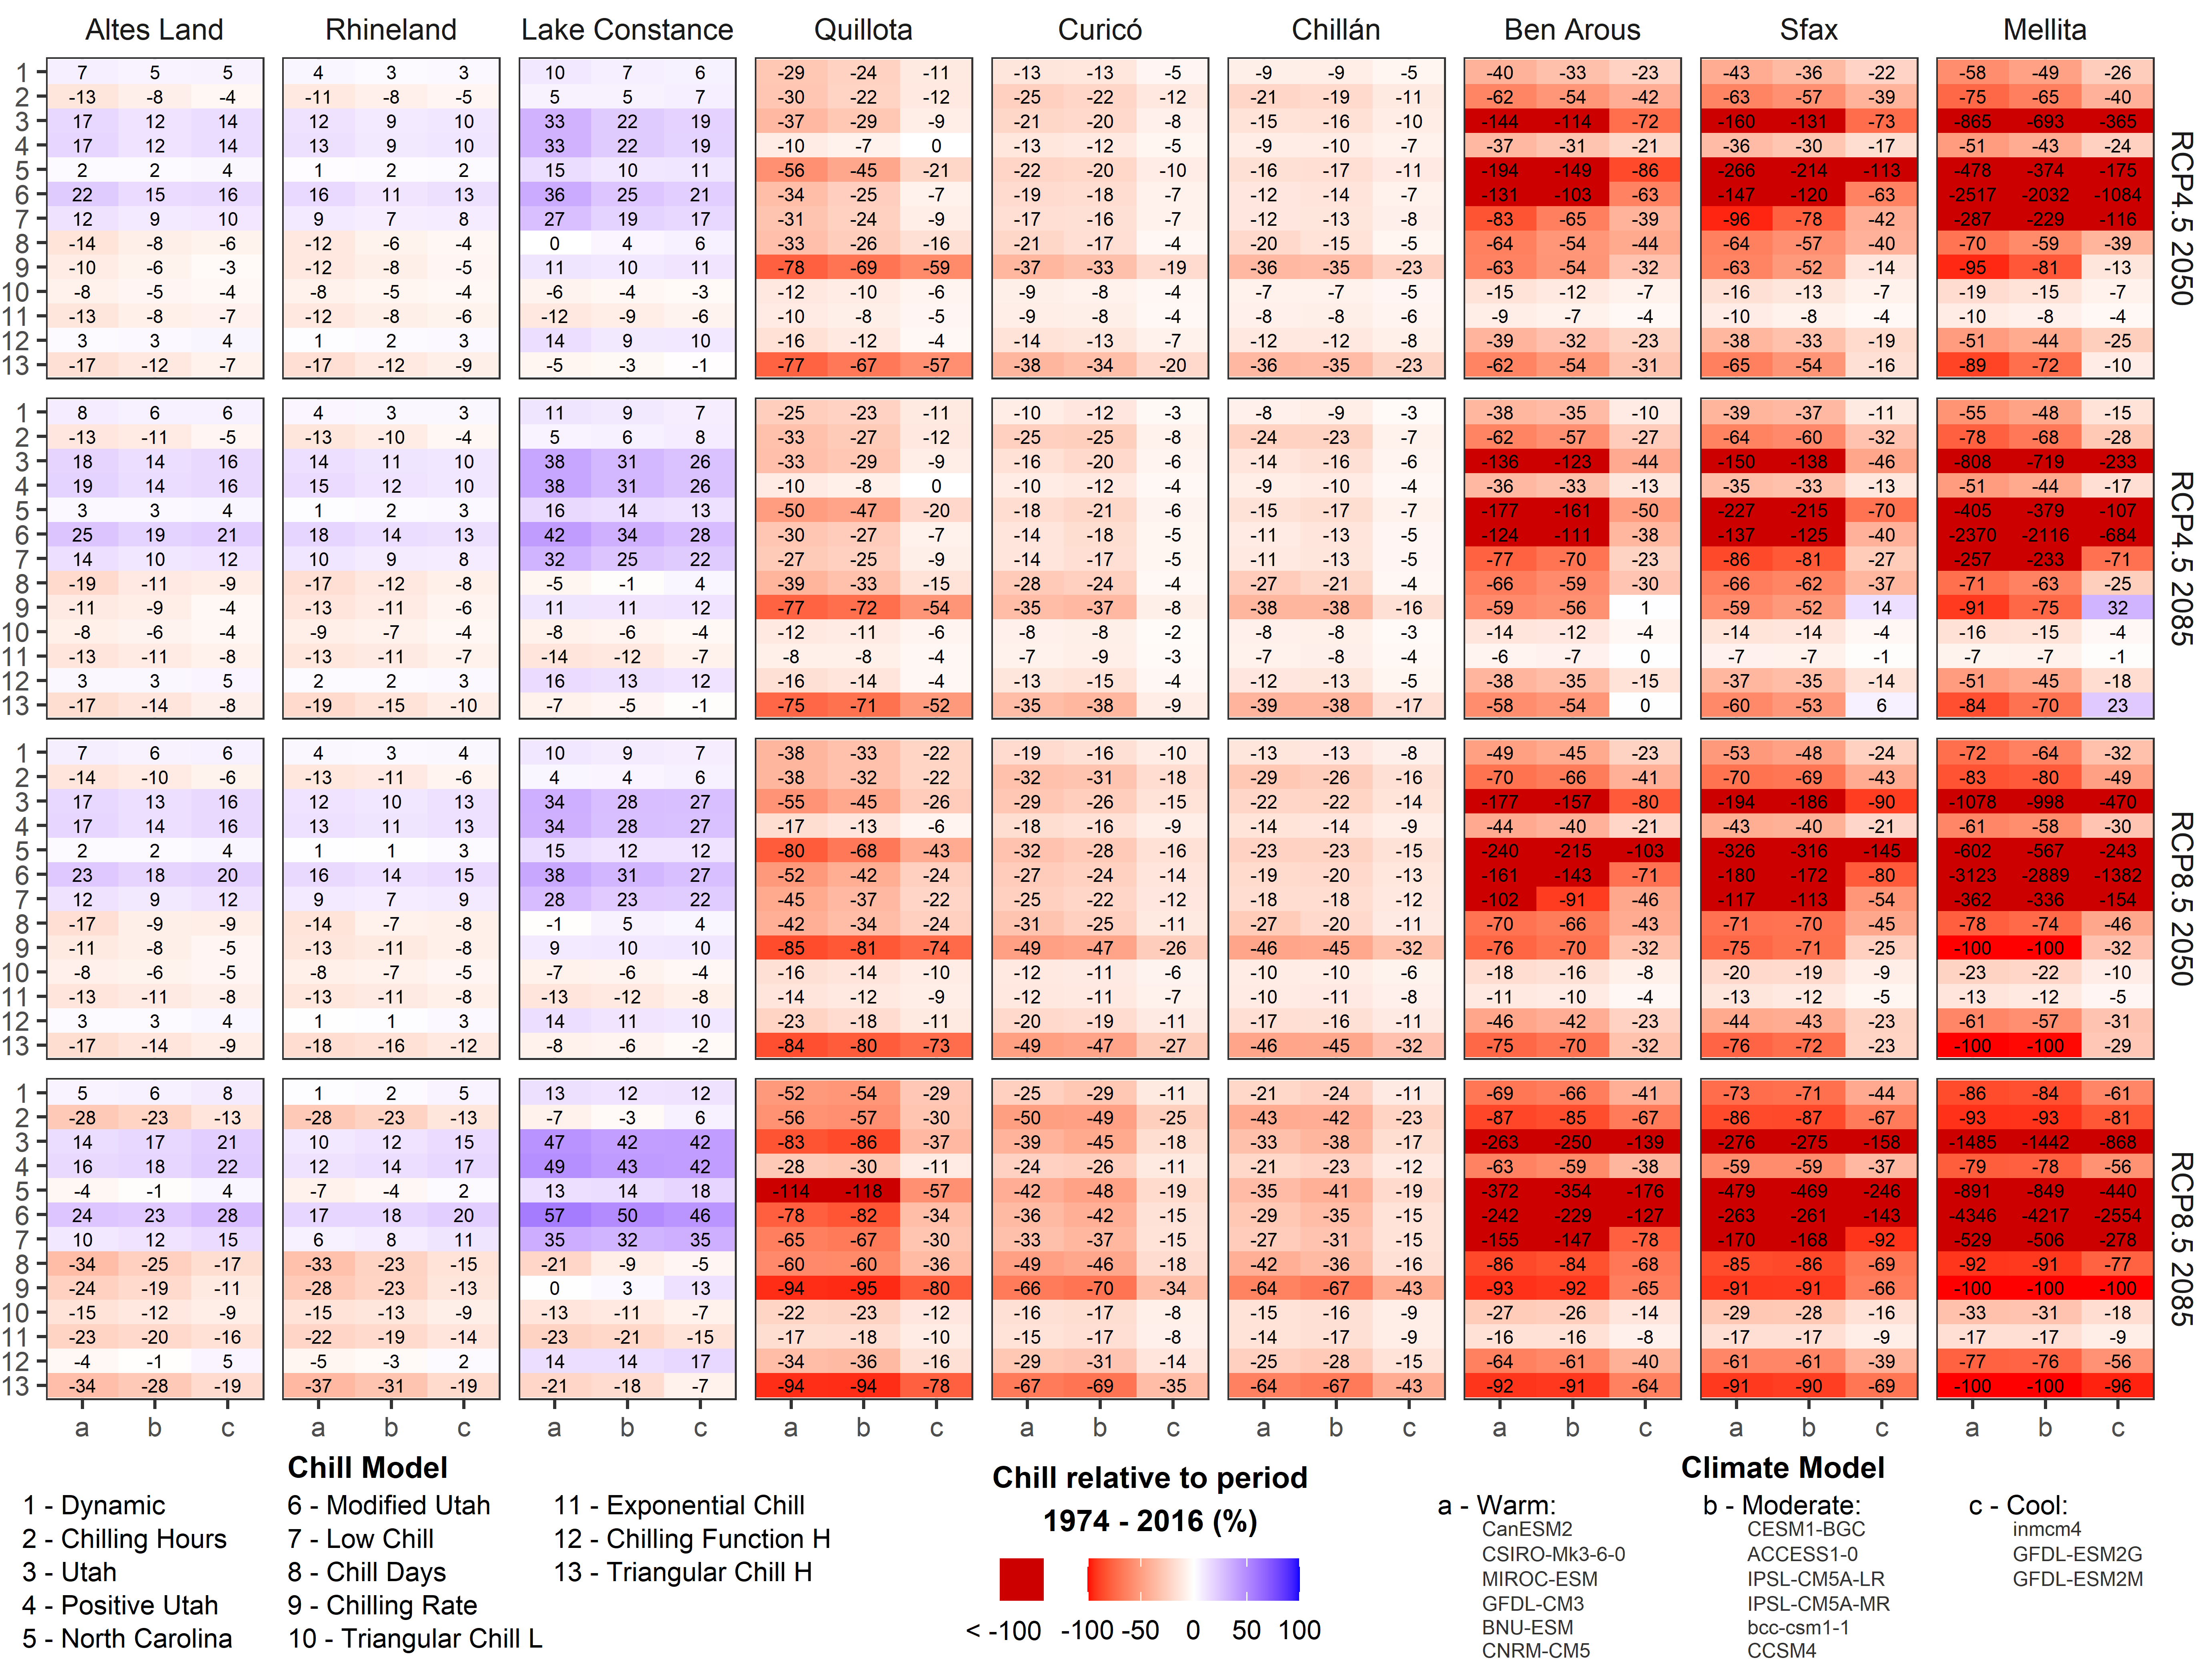
\includegraphics[width=0.9\textwidth,height=\textheight]{pictures/Model_comp_results.png}
\caption{Locations used for comparing predictions by a total of 13 chill models across different climates}
\end{figure}

This figure shows the changes predicted by the 13 models (y-axes) across various sites and climate scenarios. Note that Eduardo already did a lot of data compression here, categorizing the various climate models into three categories (warm, moderate and cool), and summarizing across all models in each of the classes. What we see here should be pretty disturbing for everyone who (like me, a decade ago) simply chooses the most convenient model for predicting something. This analysis reveals massive differences across the models! This can easily be seen by comparing the color distribution across the rows in each of the panels. A set of equivalent models would have produced the same shade of red or blue for each column of the plots in this figure. The result we obtained is far from that, showing huge differences in model predictions. For locations in Tunisia and Chile, this variation mainly concerns the extent of chill losses, with predictions ranging from rather mild to alarming. For locations in Germany, not even the direction of change is clear, with some models predicting increases, others decreases in available chill.

These results clearly indicate that \textbf{model choice matters}! Fortunately, many of these models seem rather arbitrary and can easily be dismissed. Yet there surely is residual uncertainty about which of these models, if any, makes the right calls. This is an active field of research that creative minds can/will make meaningful contributions to in the future.

\hypertarget{chill-projection-for-all-of-tunisia}{%
\subsection{Chill projection for all of Tunisia}\label{chill-projection-for-all-of-tunisia}}

As mentioned above, we projected climate change impacts on winter chill for an orchard near Sfax in Central Tunisia \href{https://link.springer.com/article/10.1007/s00484-018-1628-x}{(Benmoussa et al. \protect\hyperlink{ref-benmoussa2018climate}{2018})}. This is, however, not the most interesting region in the country for growing temperate fruit and nut trees. Despite its rather modest size, Tunisia is a climatically diverse country, with mountains and plains, coastal areas and interior deserts. Historic and future chill availability therefore shows considerable variation within the country.

Led by Haifa Benmoussa, we mapped chill accumulation across Tunisia, based on the framework we've already encountered \href{https://link.springer.com/article/10.1007/s10584-020-02774-7}{(Benmoussa et al. \protect\hyperlink{ref-benmoussa2020severe}{2020})} This analysis was based on 20 weather station locations across Tunisia and neighboring countries. By now, you probably have a pretty good idea of how we did this analysis - we just applied the analysis framework we developed to each of the 20 locations. In addition to the site-specific analysis we had produced earlier, we were now able to interpolate our results to produce chill maps that track chill availability in Tunisia over the past few decades:

\begin{figure}
\centering
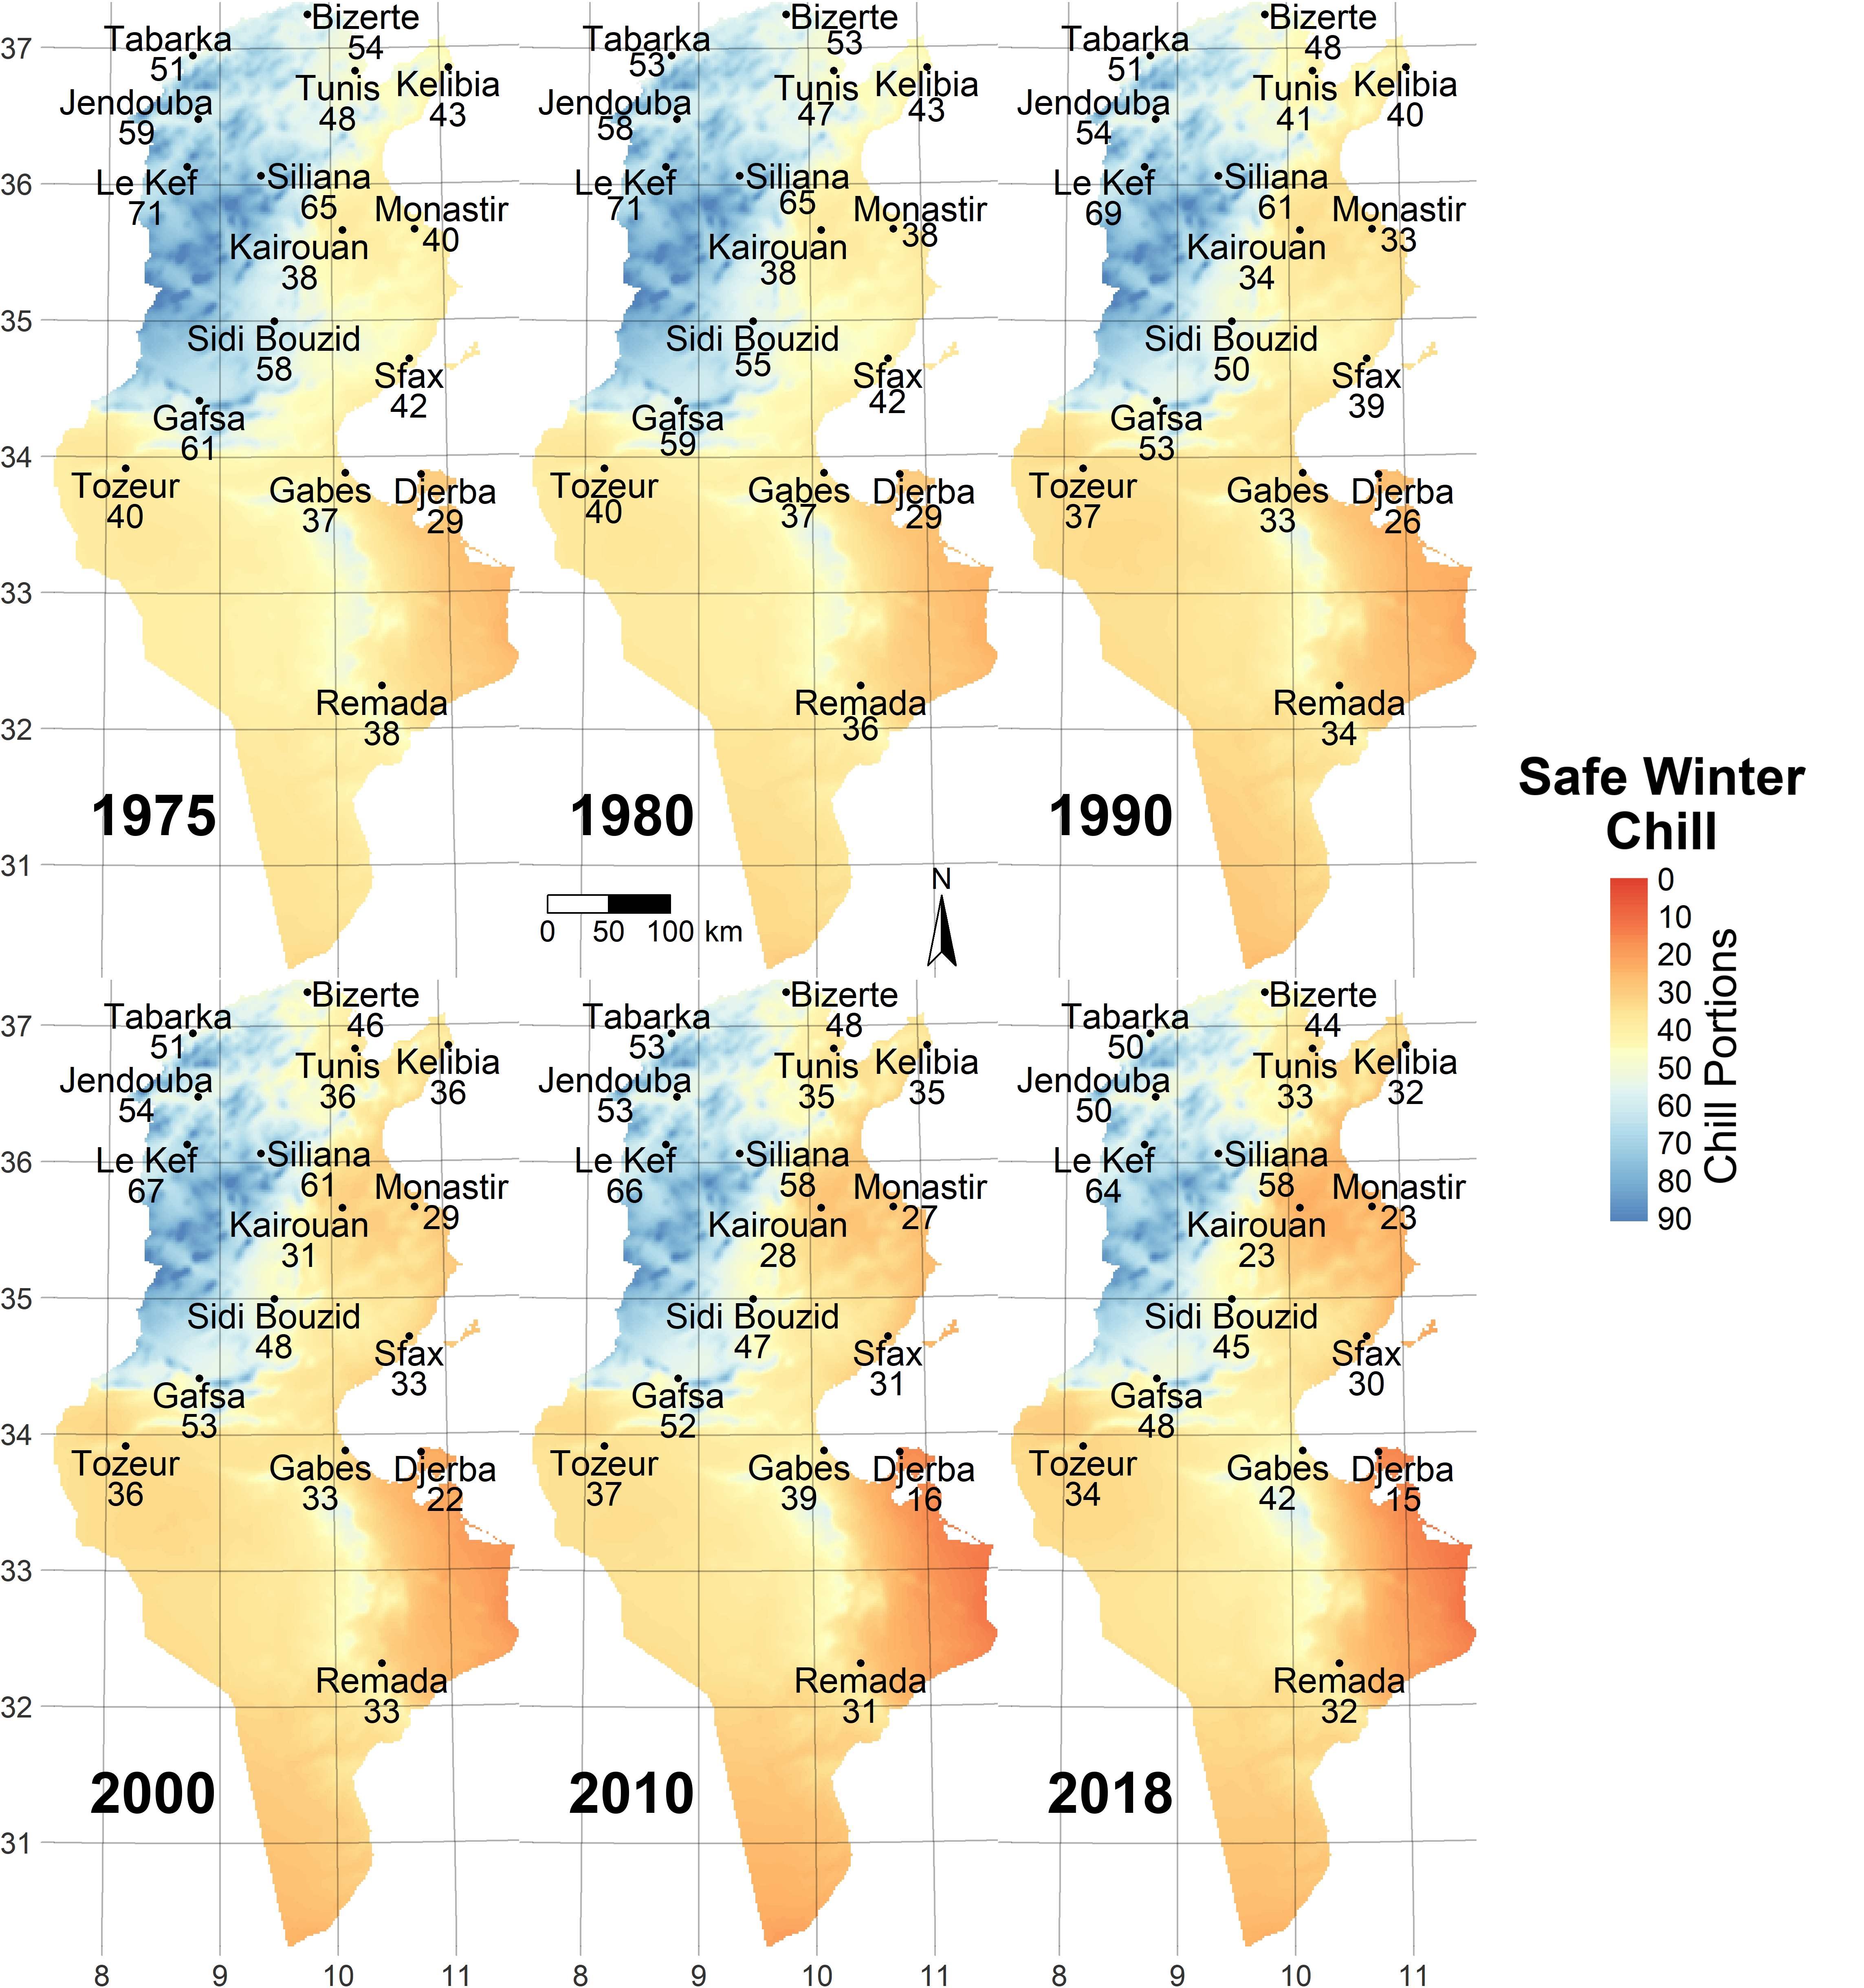
\includegraphics[width=0.9\textwidth,height=\textheight]{pictures/Figure_1_Tunisia_historic.png}
\caption{Chill availability maps for Tunisia for several past scenarios}
\end{figure}

You may wonder here how we managed to interpolate the site-specific results into a map that covers the whole country. Well, this is an area that we may still make some improvements in. The current procedure, which is probably not perfect yet, is that we take the site-specific predictions of Safe Winter Chill (remember that's the 10\textsuperscript{th} percentile of the chill distribution derived from the `replicates' of annual temperature dynamics produced by the weather generator), and interpolate a surface through them (using the Kriging technique). We did the same for the elevations of the locations we modeled chill for. We then fitted a linear model to relate chill accumulation to elevation. Making use of a Digital Elevation Model (DEM), we were able to calculate the difference between the elevation model derived from the weather station elevations and the \emph{true} elevations of each location of the country. Considering that this difference is not yet accounted for by the chill surface that was derived by interpolating chill data for the weather stations, we used the elevation\textasciitilde chill relationship we determined to correct chill predictions.

Was this confusing? Well, there's room for improvement here, and it's pretty clear that the procedure I just described will only work in places with a linear relationship between elevation and chill availability. This seems a fairly reasonable assumption in Tunisia, but it would not work in many cooler locations, such as Germany.

Here's the projection of future chill we produced for Tunisia:

\begin{figure}
\centering
\includegraphics[width=0.9\textwidth,height=\textheight]{pictures/Figure_2_Tunisia_all_scenarios.png}
\caption{Chill availability for Tunisia for various plausible scenarios of future climate}
\end{figure}

What we see here is pretty concerning. The Dynamic Model, which we used to predict chill here, is considered rather credible, and we're seeing massive decreases in Chill Portions, the units the Dynamic Model uses. This is bad news for most of Tunisia! Note that even in the places where we expect substantial winter chill to remain, farmers will likely have to adapt, because the trees they grow are aligned with the climate of the past. Adaptation strategies may involve transitioning to tree cultivars with low chilling requirements (if such cultivars are available).

\hypertarget{revisiting-chill-accumulation-in-oman}{%
\subsection{Revisiting chill accumulation in Oman}\label{revisiting-chill-accumulation-in-oman}}

After a decade of foraging in other parts of the world, let's come back to Oman. I'd long been a bit dissatisfied with the initial work we did there. Note that the first analysis was my first study on chill accumulation. At the time, I did not know about the hazards involved in model choice. I also didn't have proper data on projected future climates then, and the process that converted daily to hourly temperatures was quite a bit less than ideal.

My PhD supervisor and mentor \href{https://scholar.google.de/citations?user=ZNvcJJ8AAAAJ\&hl=de}{Prof.~Dr.~Andreas Bürkert} had pushed me for quite some time to redo the analysis for Oman. With our climate change analysis framework, we could finally do it. Adding some new ideas on how to convert daily into hourly temperatures in a place like the oases of Oman we were interested in (you'll learn about these ideas later in this module), we produced updated assessments of past winter chill and forecasts of future chill for the oases of Al Jabal Al Akhdar. The results have just come out \href{https://link.springer.com/article/10.1007/s10584-020-02862-8}{(Buerkert et al. \protect\hyperlink{ref-buerkert2020revisiting}{2020})}.

\hypertarget{future-studies}{%
\subsection{Future studies?}\label{future-studies}}

Now we've reached the present. By now you should have a pretty good overview of the state of the art in chill modeling (or the modeling of climate change impacts on any temperature-related phenomenon). By the end of this module, you should be able to do such analyses yourself. The next steps will be up to you!

\hypertarget{exercises_past_studies}{%
\section*{\texorpdfstring{\texttt{Exercises} on past chill projections}{Exercises on past chill projections}}\label{exercises_past_studies}}
\addcontentsline{toc}{section}{\texttt{Exercises} on past chill projections}

Please document all results of the following assignments in your \texttt{learning\ logbook}.

\begin{enumerate}
\def\labelenumi{\arabic{enumi})}
\item
  Sketch out three data access and processing challenges that had to be overcome in order to produce chill projections with state-of-the-art methodology.
\item
  Outline, in your understanding, the basic steps that are necessary to make such projections.
\end{enumerate}

\hypertarget{manual-chill-analysis}{%
\chapter{Manual chill analysis}\label{manual-chill-analysis}}

\hypertarget{goals_manual_chill_analysis}{%
\section*{Learning goals for this lesson}\label{goals_manual_chill_analysis}}
\addcontentsline{toc}{section}{Learning goals for this lesson}

\begin{itemize}
\tightlist
\item
  Learn about some basic R operations we need for calculating Chilling Hours
\item
  Be able to calculate Chilling Hours
\item
  Understand what an R function is
\item
  Be able to write your own basic function
\end{itemize}

\hypertarget{computing-chilling-hours-from-hourly-temperature-data}{%
\section{Computing Chilling Hours from hourly temperature data}\label{computing-chilling-hours-from-hourly-temperature-data}}

Basic chill models like the Chilling Hours Model aren't particularly complicated, so it's not so hard to calculate chill manually (at least not if you're familiar with R, or even a spreadsheet program). So we're going to try this here to gain some understanding of what the respective functions in the \texttt{chillR} package do.

One important challenge that most people who want to compute Chilling Hours quickly realize is that we need hourly temperature data. Quite often, this isn't available, and that's already where the problems start. For now, we're going to ignore this problem and work with data that already has an hourly time step. A bit later, we'll talk about ways to make pretty good approximations of hourly temperature data from daily records, for which \texttt{chillR} offers a few neat tools.

Let me first say that I always have to swallow a toad when I use Chilling Hours, because I don't think they are very useful. They are, however, the chill model that is most widely known, they are very easy to explain, and they are not hard to calculate. Since at this point we're absolute beginners in chill modeling, let's start there.

First, we have to get data into R. The most obvious way to achieve this is reading a data table into R with the \texttt{read.table} or \texttt{read.csv} functions. There are also packages that can read in \texttt{.xls} or \texttt{.xlsx} files.

For this initial example, we won't do this, but work with a sample dataset that comes with \texttt{chillR}. The package contains the dataset \texttt{winters\_hours\_gaps}, which was recorded in a walnut orchard near Winters, California, in 2008. You can get some impressions of the settings here:

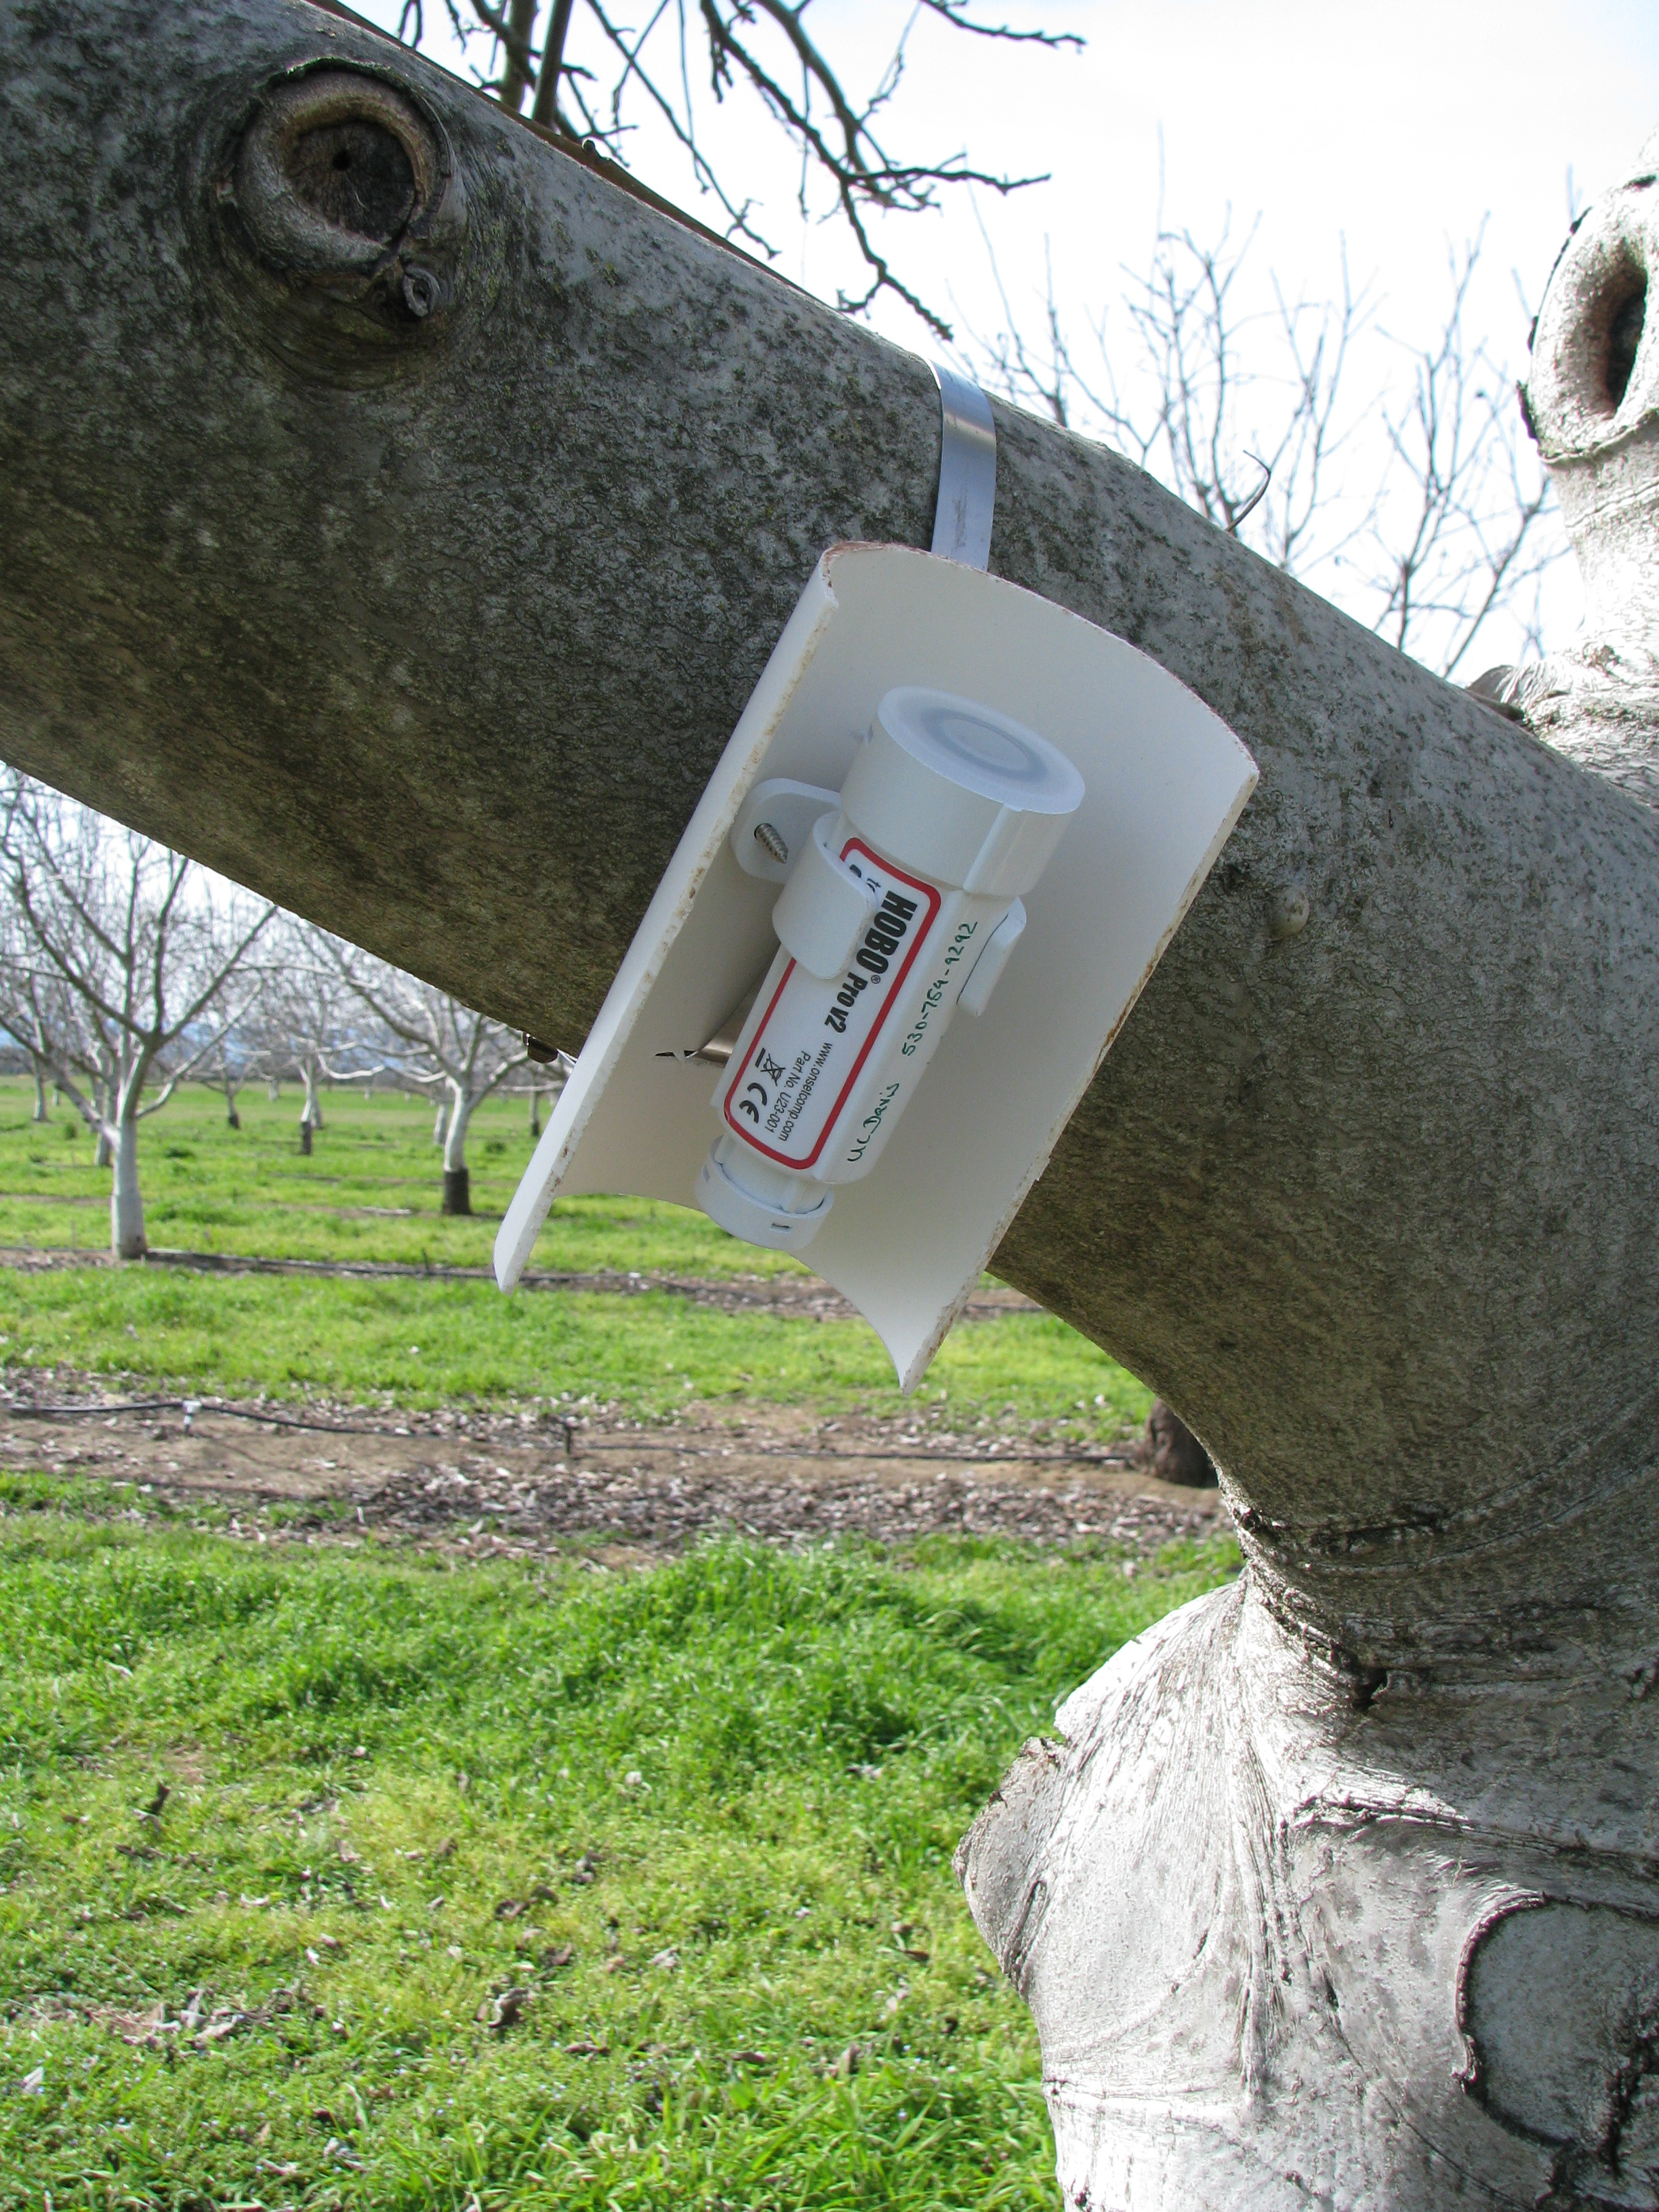
\includegraphics[width=0.33\textwidth,height=\textheight]{pictures/Walnuts_March.JPG} 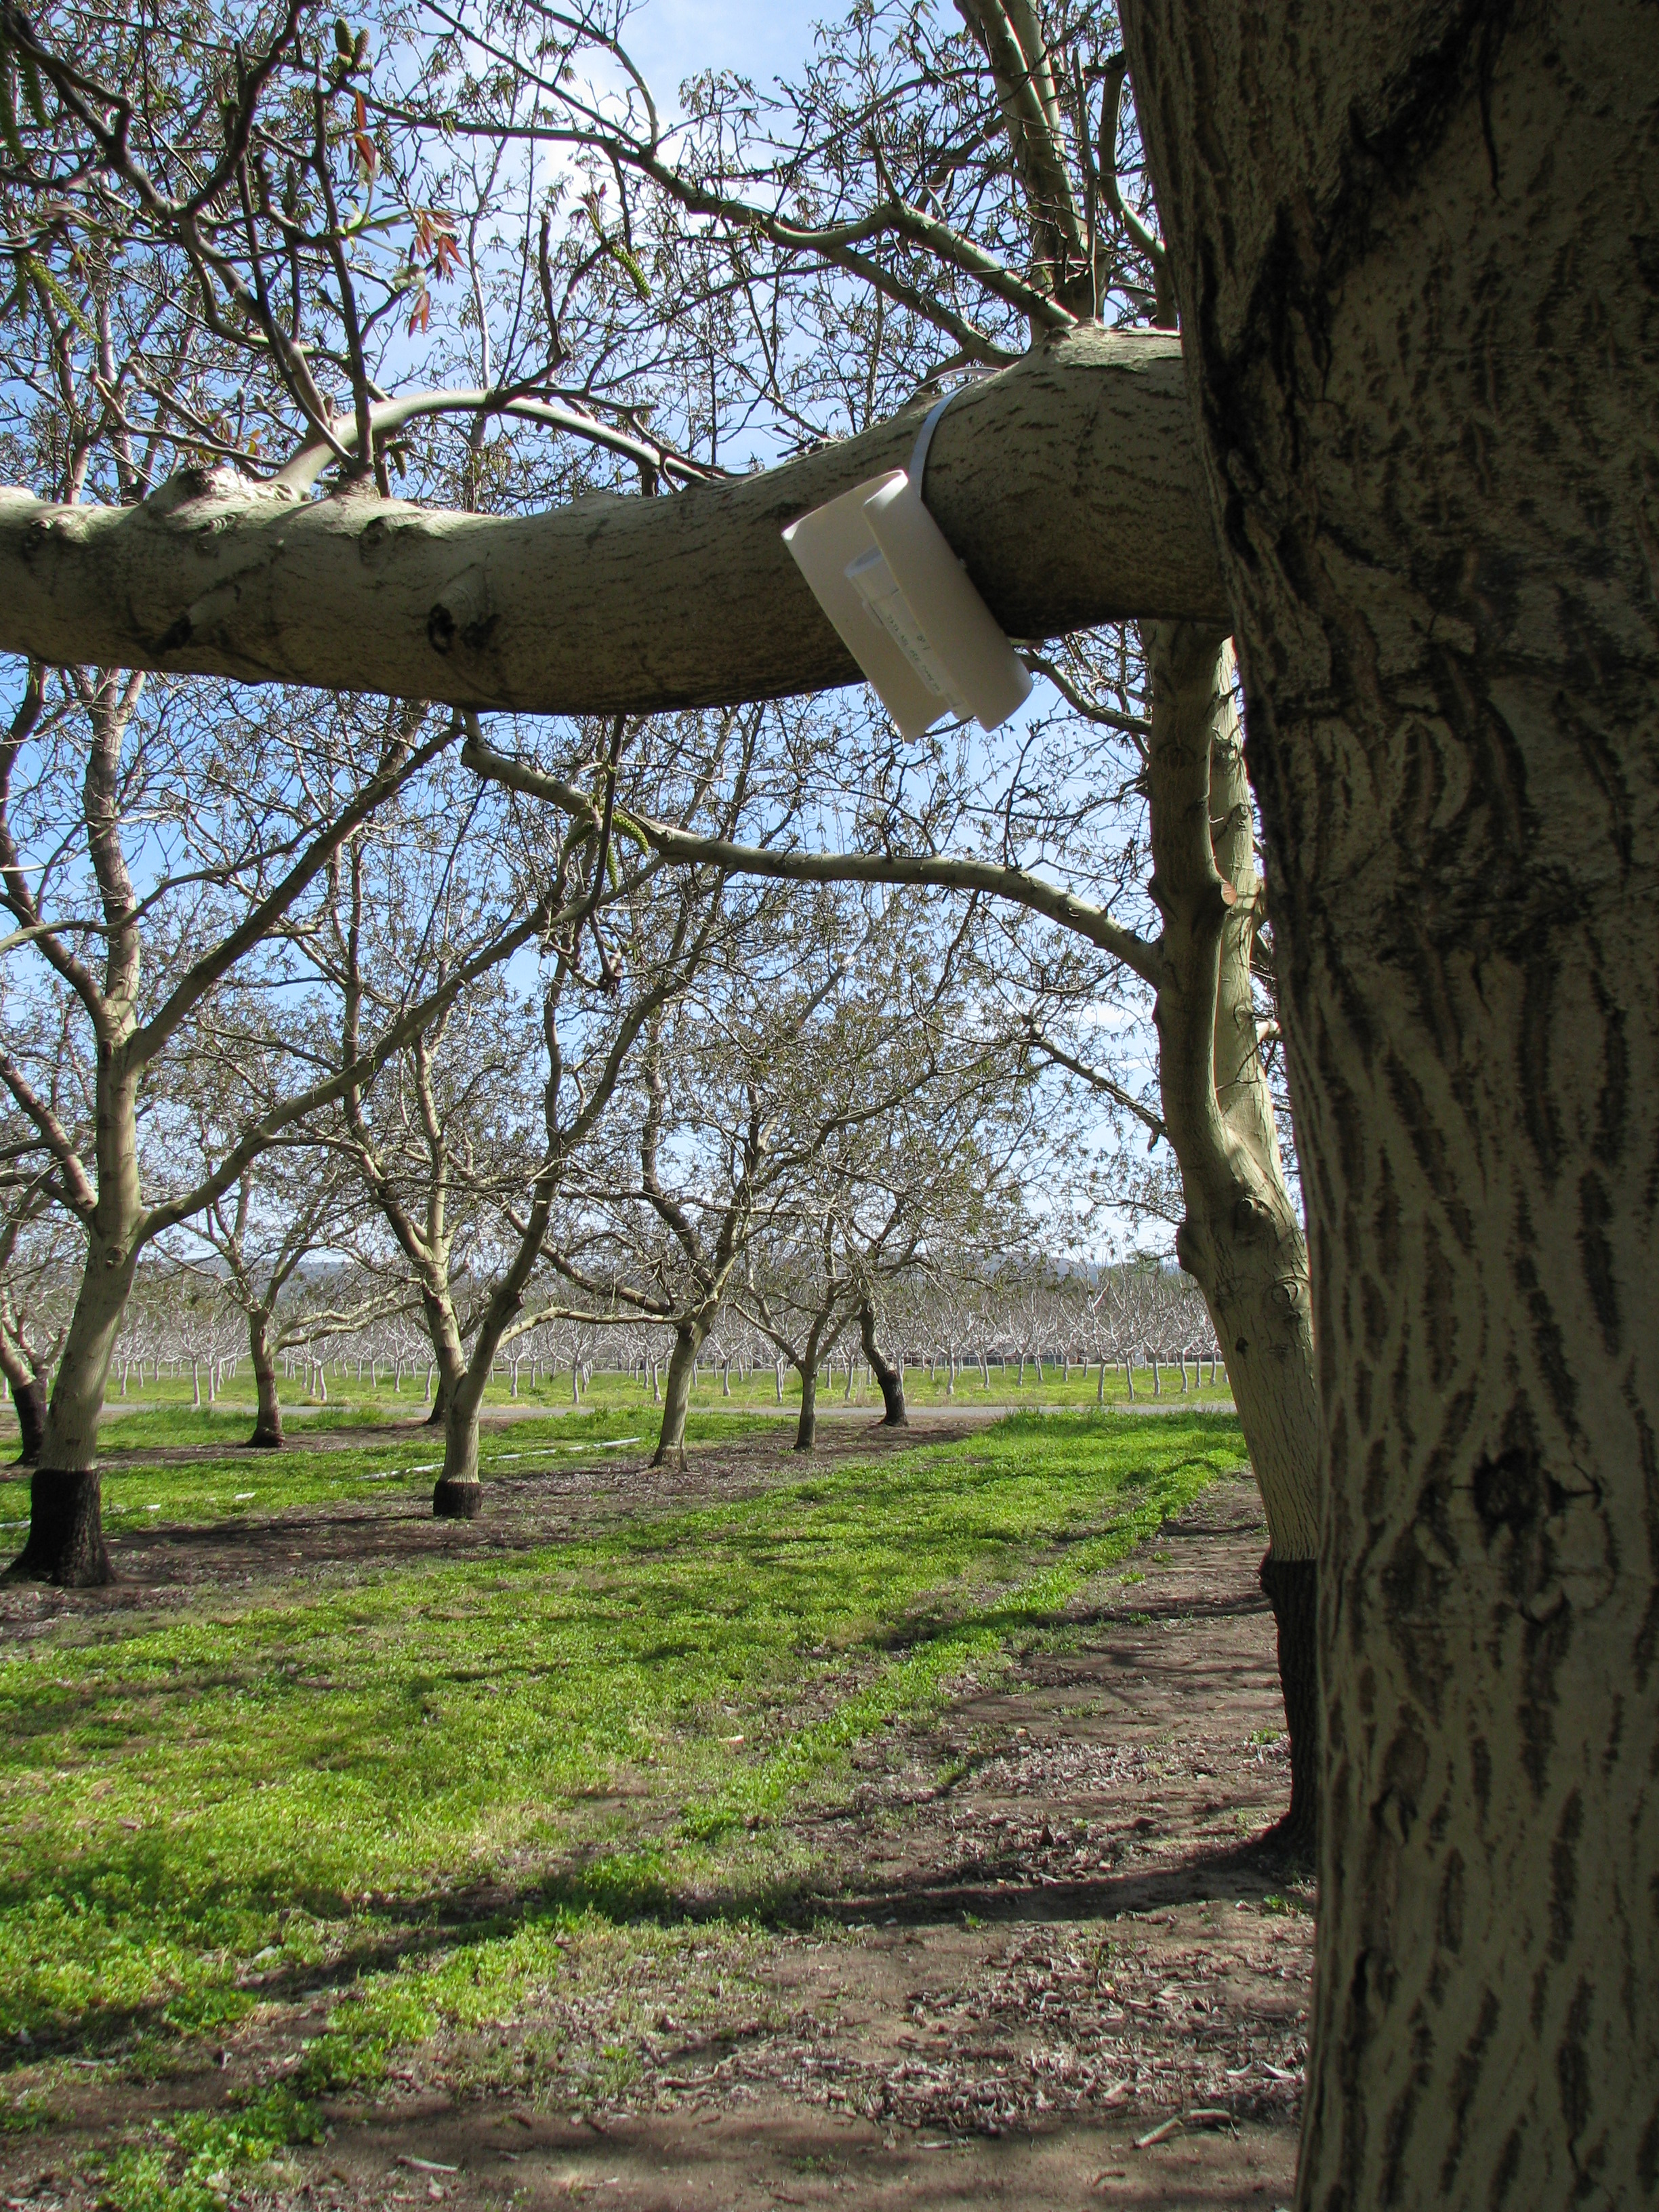
\includegraphics[width=0.33\textwidth,height=\textheight]{pictures/Walnuts_April.JPG} 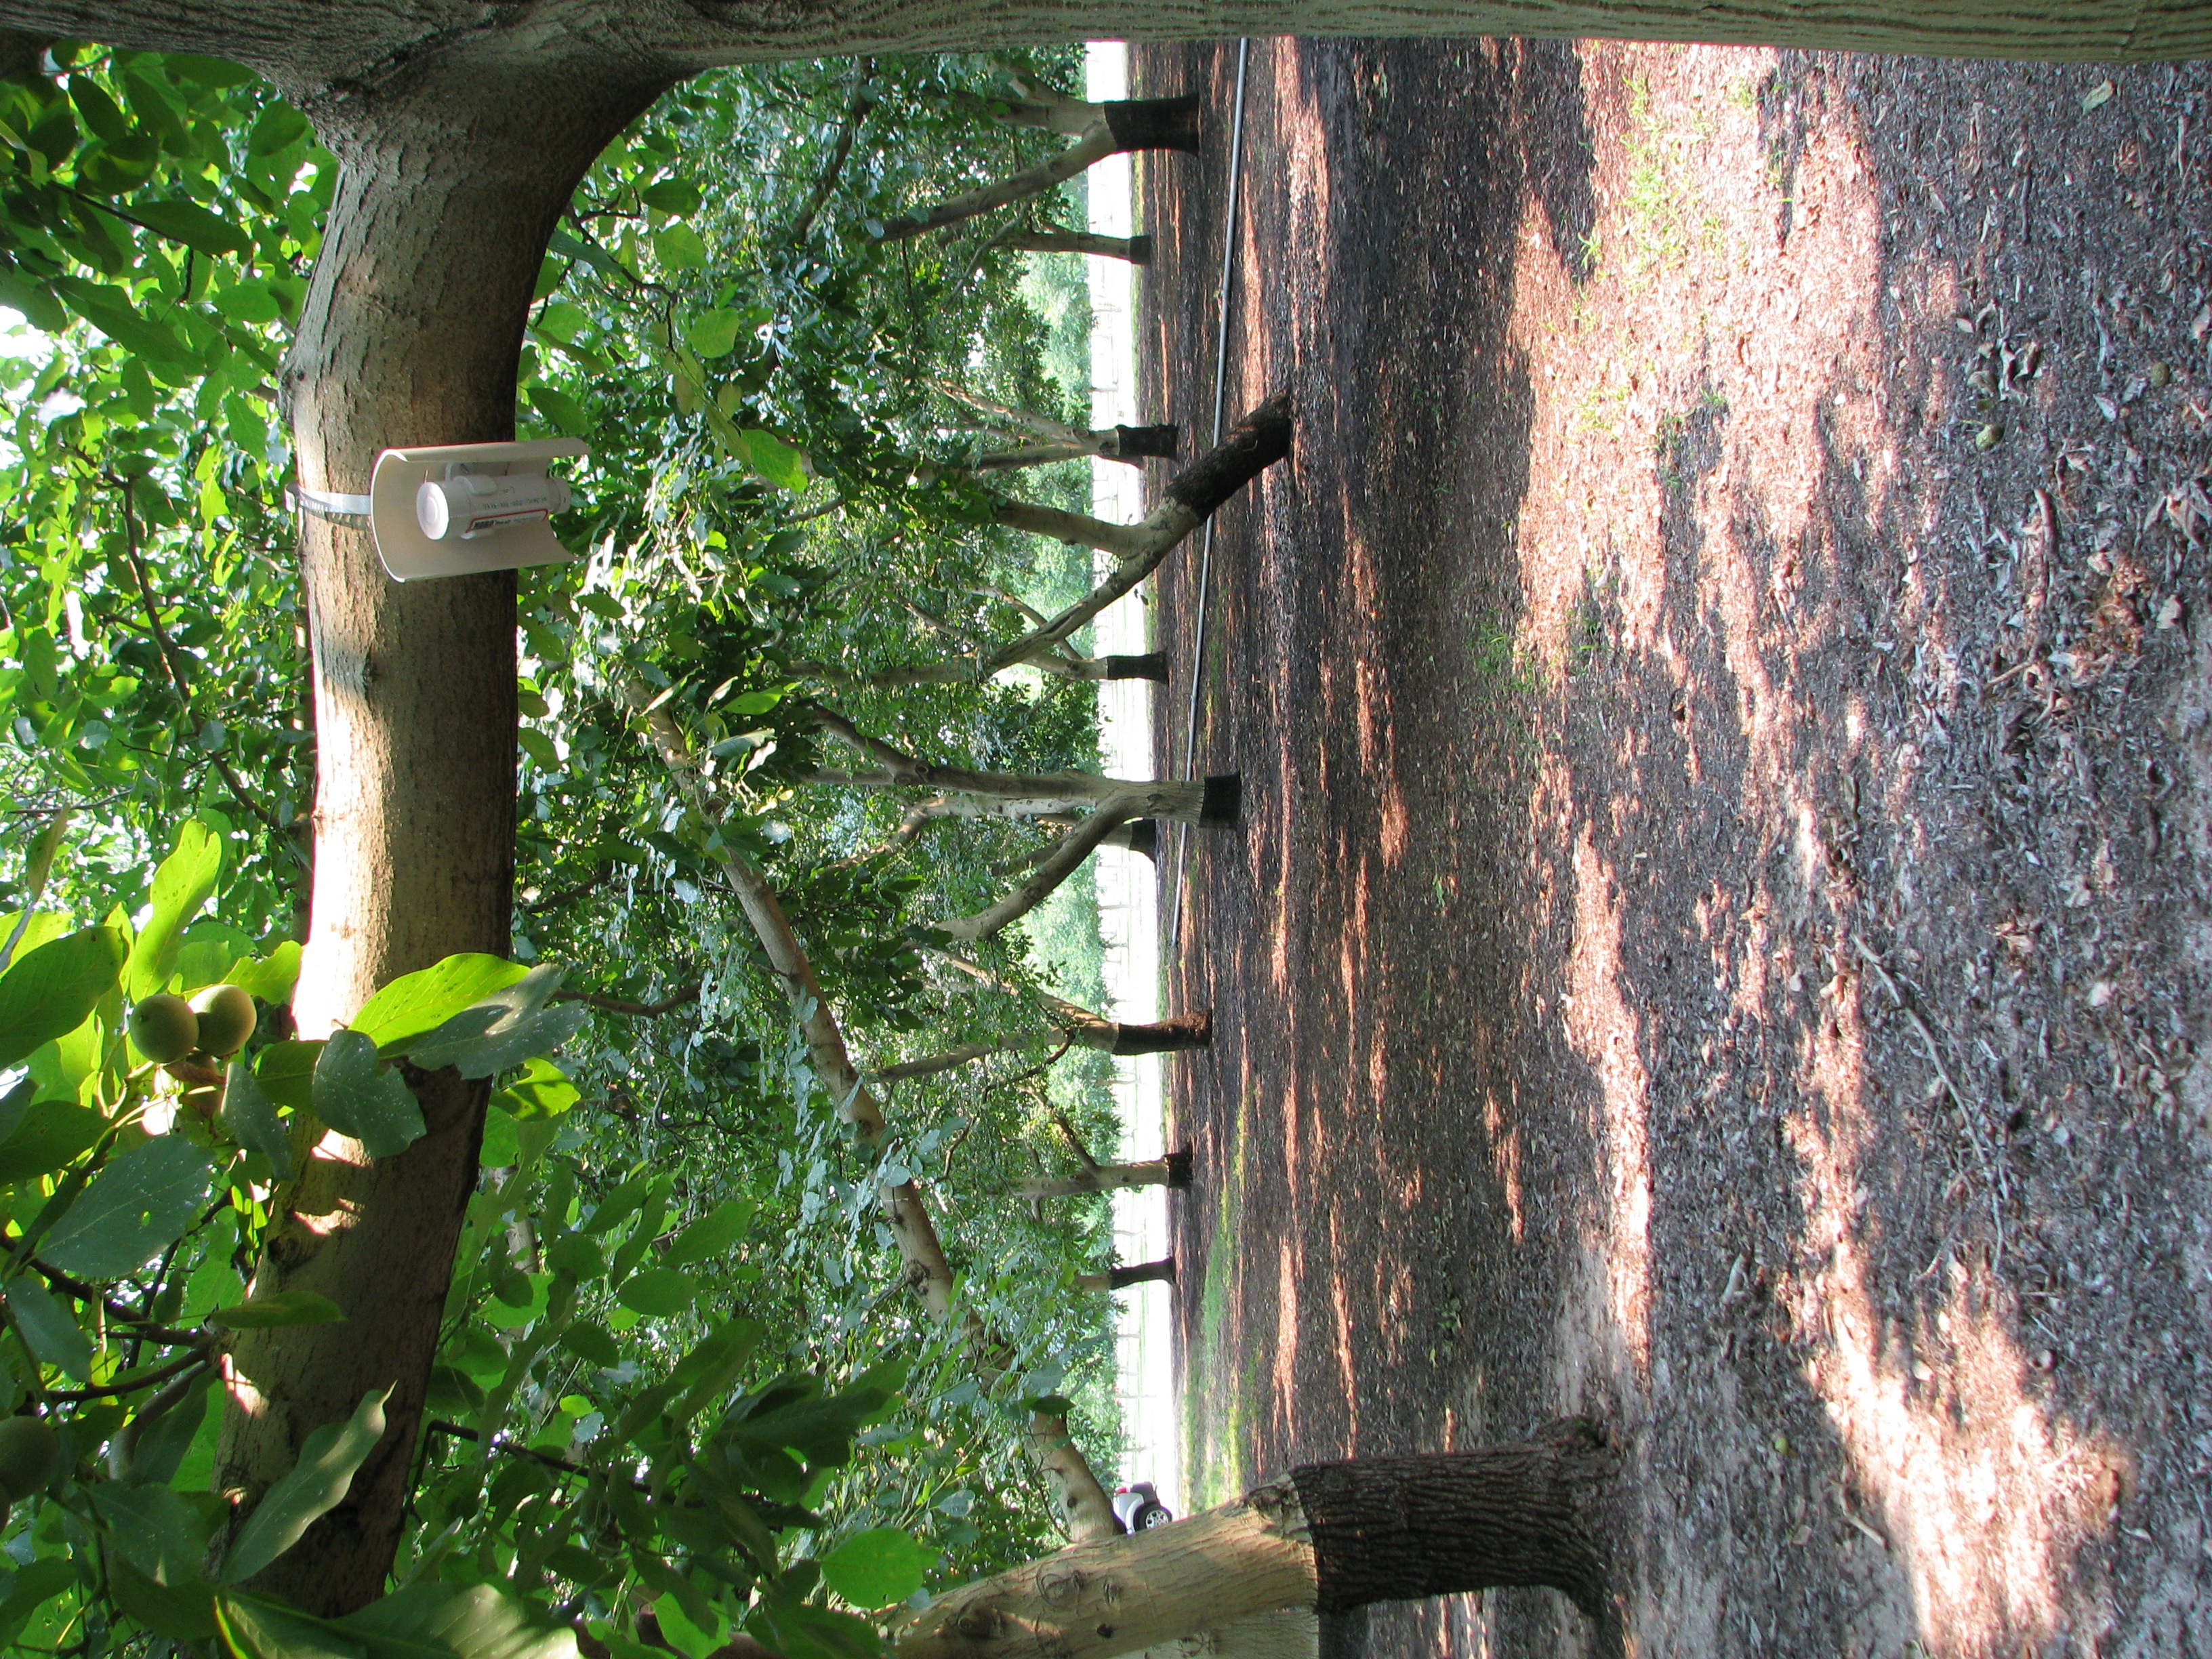
\includegraphics[width=0.33\textwidth,height=\textheight]{pictures/Walnuts_May.JPG}

These three pictures were taken between March and May of 2008. Note how the light conditions change over time. This impacts the daily temperature dynamics, which we'll talk about in one of the next chapters

To gain access to the \texttt{winters\_hours\_gaps} dataset, and to all other functionality in the \texttt{chillR} package, we have to first install and load \texttt{chillR}.

Note that in the call below, the \texttt{install.packages} command is `commented out' by the hashtag (\#). This means that the respective line isn't evaluated. If you haven't installed `chillR' yet, you'll have to run this line without the \#. I'm also loading a couple of additional packages (\texttt{knitr}, \texttt{pander}) that are needed for making the website you're looking at.

\begin{Shaded}
\begin{Highlighting}[]
\CommentTok{#install.packages("chillR")}
\KeywordTok{library}\NormalTok{(chillR)}
\KeywordTok{library}\NormalTok{(knitr)}
\KeywordTok{library}\NormalTok{(pander)}
\KeywordTok{library}\NormalTok{(kableExtra)}
\end{Highlighting}
\end{Shaded}

\begin{verbatim}
## 
## Attaching package: 'kableExtra'
\end{verbatim}

\begin{verbatim}
## The following object is masked from 'package:dplyr':
## 
##     group_rows
\end{verbatim}

\begin{Shaded}
\begin{Highlighting}[]
\KeywordTok{kable}\NormalTok{(Winters_hours_gaps[}\DecValTok{1}\OperatorTok{:}\DecValTok{10}\NormalTok{,])  }\OperatorTok
\StringTok{  }\KeywordTok{kable_styling}\NormalTok{(}\StringTok{"striped"}\NormalTok{, }\DataTypeTok{position =} \StringTok{"left"}\NormalTok{,}\DataTypeTok{font_size =} \DecValTok{10}\NormalTok{)}
\end{Highlighting}
\end{Shaded}

\begingroup\fontsize{10}{12}\selectfont

\begin{tabular}{r|r|r|r|r|r}
\hline
Year & Month & Day & Hour & Temp\_gaps & Temp\\
\hline
2008 & 3 & 3 & 10 & 15.127 & 15.127\\
\hline
2008 & 3 & 3 & 11 & 17.153 & 17.153\\
\hline
2008 & 3 & 3 & 12 & 18.699 & 18.699\\
\hline
2008 & 3 & 3 & 13 & 18.699 & 18.699\\
\hline
2008 & 3 & 3 & 14 & 18.842 & 18.842\\
\hline
2008 & 3 & 3 & 15 & 19.508 & 19.508\\
\hline
2008 & 3 & 3 & 16 & 19.318 & 19.318\\
\hline
2008 & 3 & 3 & 17 & 17.701 & 17.701\\
\hline
2008 & 3 & 3 & 18 & 15.414 & 15.414\\
\hline
2008 & 3 & 3 & 19 & 12.727 & 12.727\\
\hline
\end{tabular}
\endgroup{}

\begin{Shaded}
\begin{Highlighting}[]
\NormalTok{hourtemps<-Winters_hours_gaps[,}\KeywordTok{c}\NormalTok{(}\StringTok{"Year"}\NormalTok{,}\StringTok{"Month"}\NormalTok{,}\StringTok{"Day"}\NormalTok{,}\StringTok{"Hour"}\NormalTok{,}\StringTok{"Temp"}\NormalTok{)]}
\end{Highlighting}
\end{Shaded}

This code loaded \texttt{chillR}, showed us what the \texttt{Winters\_hours\_gaps} dataset looks like (using the \texttt{kable} format, which you don't need in R, but which makes the markdown output prettier - you'll learn later what this means). The dataset contains a column that we don't need (\texttt{Temps\_gaps}, which I added to demonstrate the use of a \texttt{chillR} function that can fill such gaps), so I'm creating a new dataset (\texttt{hourtemps}) that only contains the columns we want.

What we get now is the standard format of an hourly \texttt{chillR} temperature record - with separate columns for \texttt{Year}, \texttt{Month}, \texttt{Day}, \texttt{Hour} and \texttt{Temp}. The last column contains hourly temperatures (without gaps), which we can use to calculate Chilling Hours.

The data format of this dataset is a so-called \texttt{data.frame}, a structure with multiple columns and rows. We can access information in this hourtemps data.frame by referring to it as \texttt{hourtemps{[}rows,column{]}}. Here \texttt{row} can be a number, a range of numbers (e.g.~\texttt{c(1,2,4)}, \texttt{1:5}), or even a name, if you're using the option to assign names to rows (we're not doing that here). \texttt{column} is the same for the columns, except that for this we are using names (e.g.~\texttt{Year}, \texttt{Temp}). If you want all rows (columns), leave the column (row) argument blank. To refer to a row, you can also add the name directly after the data.frame name, separated by a \texttt{\$} sign.

\begin{Shaded}
\begin{Highlighting}[]
\NormalTok{hourtemps[}\DecValTok{3}\NormalTok{,]}
\end{Highlighting}
\end{Shaded}

\begin{verbatim}
##   Year Month Day Hour   Temp
## 3 2008     3   3   12 18.699
\end{verbatim}

\begin{Shaded}
\begin{Highlighting}[]
\NormalTok{hourtemps[}\DecValTok{3}\NormalTok{,}\StringTok{"Temp"}\NormalTok{]}
\end{Highlighting}
\end{Shaded}

\begin{verbatim}
## [1] 18.699
\end{verbatim}

\begin{Shaded}
\begin{Highlighting}[]
\NormalTok{hourtemps}\OperatorTok{$}\NormalTok{Temp[}\DecValTok{1}\OperatorTok{:}\DecValTok{5}\NormalTok{]}
\end{Highlighting}
\end{Shaded}

\begin{verbatim}
## [1] 15.127 17.153 18.699 18.699 18.842
\end{verbatim}

\begin{Shaded}
\begin{Highlighting}[]
\NormalTok{hourtemps[}\DecValTok{1}\OperatorTok{:}\DecValTok{5}\NormalTok{,]}
\end{Highlighting}
\end{Shaded}

\begin{verbatim}
##   Year Month Day Hour   Temp
## 1 2008     3   3   10 15.127
## 2 2008     3   3   11 17.153
## 3 2008     3   3   12 18.699
## 4 2008     3   3   13 18.699
## 5 2008     3   3   14 18.842
\end{verbatim}

To assign new values to R objects, you can use the \texttt{\textless{}-} sign. You already saw an example of this above, where the \texttt{hourtemps} data.frame was defined. You can also use such an assignment to create a new column in a data.frame. To do this, you just assign new values to a column with the name of your choice \texttt{hourtemps{[},"myColumn"{]}\textless{}-NA}. \texttt{NA} means `not available'. It's R's way of saying there's no data here. But let's directly jump to a more useful example that will set us on the path to calculating Chilling Hours.

We've already talked about Chilling Hours, but here's a reminder of what they are: Every hour with temperatures above (and including) 0°C and below (and including) 7.2°C is considered a Chilling Hour.

So what we have to do is check for every hour whether temperatures fall in this range. Such checks can be implemented in R with fairly simple comparison commands (\texttt{\textless{}}, \texttt{\textless{}=}, \texttt{==}, \texttt{=\textgreater{}} and \texttt{\textgreater{}}). These can be applied to single numbers, or to so-called \texttt{vectors}, which are strings of numbers (such as the ones created by the \texttt{c()} command - we already used this above). We can combine multiple such comparisons with the \texttt{\&} command.

\begin{Shaded}
\begin{Highlighting}[]
\DecValTok{1}\OperatorTok{==}\DecValTok{2}
\end{Highlighting}
\end{Shaded}

\begin{verbatim}
## [1] FALSE
\end{verbatim}

\begin{Shaded}
\begin{Highlighting}[]
\DecValTok{1}\OperatorTok{==}\DecValTok{1}
\end{Highlighting}
\end{Shaded}

\begin{verbatim}
## [1] TRUE
\end{verbatim}

\begin{Shaded}
\begin{Highlighting}[]
\KeywordTok{c}\NormalTok{(}\DecValTok{1}\NormalTok{,}\DecValTok{2}\NormalTok{,}\DecValTok{3}\NormalTok{)}\OperatorTok{>}\DecValTok{2}
\end{Highlighting}
\end{Shaded}

\begin{verbatim}
## [1] FALSE FALSE  TRUE
\end{verbatim}

\begin{Shaded}
\begin{Highlighting}[]
\NormalTok{a<-}\DecValTok{1}
\NormalTok{b<-}\DecValTok{2}
\NormalTok{c<-}\DecValTok{3}
\KeywordTok{c}\NormalTok{(a,b,c)}\OperatorTok{>=}\DecValTok{2}
\end{Highlighting}
\end{Shaded}

\begin{verbatim}
## [1] FALSE  TRUE  TRUE
\end{verbatim}

\begin{Shaded}
\begin{Highlighting}[]
\KeywordTok{c}\NormalTok{(a,b,c)}\OperatorTok{>=}\DecValTok{2}\OperatorTok{&}\KeywordTok{c}\NormalTok{(a,b,c)}\OperatorTok{<}\DecValTok{3}
\end{Highlighting}
\end{Shaded}

\begin{verbatim}
## [1] FALSE  TRUE FALSE
\end{verbatim}

So now we want to check if temperatures in a given hour are within the range considered to be effective for chill accumulation by the Chilling Hours Model. We then want to assign this result to a new column \texttt{Chilling\_Hour}.

\begin{Shaded}
\begin{Highlighting}[]
\NormalTok{hourtemps[,}\StringTok{"Chilling_Hour"}\NormalTok{]<-hourtemps}\OperatorTok{$}\NormalTok{Temp}\OperatorTok{>=}\DecValTok{0}\OperatorTok{&}\NormalTok{hourtemps}\OperatorTok{$}\NormalTok{Temp}\OperatorTok{<=}\FloatTok{7.2}

\NormalTok{hourtemps[}\DecValTok{13}\OperatorTok{:}\DecValTok{20}\NormalTok{,]}
\end{Highlighting}
\end{Shaded}

\begin{verbatim}
##    Year Month Day Hour  Temp Chilling_Hour
## 13 2008     3   3   22 9.040         FALSE
## 14 2008     3   3   23 7.920         FALSE
## 15 2008     3   4    0 6.535          TRUE
## 16 2008     3   4    1 6.687          TRUE
## 17 2008     3   4    2 8.767         FALSE
## 18 2008     3   4    3 9.139         FALSE
## 19 2008     3   4    4 6.788          TRUE
## 20 2008     3   4    5 5.076          TRUE
\end{verbatim}

I'm showing you here the rows 13-20 of the dataset, because temperatures only then reached the interesting range. The \texttt{Chilling\_Hour} column now reads \texttt{FALSE} and \texttt{TRUE}, but these values are equivalent to \texttt{0} and \texttt{1}, and we can calculate with them. It's now easy to add up the Chilling Hours of a particular period, which we can do with the \texttt{sum} command.

\begin{Shaded}
\begin{Highlighting}[]
\KeywordTok{sum}\NormalTok{(hourtemps}\OperatorTok{$}\NormalTok{Chilling_Hour[}\DecValTok{13}\OperatorTok{:}\DecValTok{20}\NormalTok{])}
\end{Highlighting}
\end{Shaded}

\begin{verbatim}
## [1] 4
\end{verbatim}

So between the 13\textsuperscript{th} and 20\textsuperscript{th} hour, we had 4 Chilling Hours. With a slightly more complex command, we can calculate chill between actual dates. We'll use the \texttt{which} command to identify the hours in the dataset that correspond to the date we're interested in.

\begin{Shaded}
\begin{Highlighting}[]
\NormalTok{Start_Date<-}\KeywordTok{which}\NormalTok{(hourtemps}\OperatorTok{$}\NormalTok{Year}\OperatorTok{==}\DecValTok{2008} \OperatorTok{&}\StringTok{ }\NormalTok{hourtemps}\OperatorTok{$}\NormalTok{Month}\OperatorTok{==}\DecValTok{10} \OperatorTok{&}
\StringTok{                    }\NormalTok{hourtemps}\OperatorTok{$}\NormalTok{Day}\OperatorTok{==}\DecValTok{1} \OperatorTok{&}\StringTok{ }\NormalTok{hourtemps}\OperatorTok{$}\NormalTok{Hour}\OperatorTok{==}\DecValTok{12}\NormalTok{)}
\NormalTok{End_Date<-}\KeywordTok{which}\NormalTok{(hourtemps}\OperatorTok{$}\NormalTok{Year}\OperatorTok{==}\DecValTok{2008} \OperatorTok{&}\StringTok{ }\NormalTok{hourtemps}\OperatorTok{$}\NormalTok{Month}\OperatorTok{==}\DecValTok{10} \OperatorTok{&}
\StringTok{                  }\NormalTok{hourtemps}\OperatorTok{$}\NormalTok{Day}\OperatorTok{==}\DecValTok{31} \OperatorTok{&}\StringTok{ }\NormalTok{hourtemps}\OperatorTok{$}\NormalTok{Hour}\OperatorTok{==}\DecValTok{12}\NormalTok{)}

\KeywordTok{sum}\NormalTok{(hourtemps}\OperatorTok{$}\NormalTok{Chilling_Hour[Start_Date}\OperatorTok{:}\NormalTok{End_Date])}
\end{Highlighting}
\end{Shaded}

\begin{verbatim}
## [1] 28
\end{verbatim}

So in October of 2008, Winters experienced 28 Chilling Hours.

\hypertarget{our-first-chill-function}{%
\section{Our first chill function}\label{our-first-chill-function}}

The code for calculating Chilling Hours wasn't very complex, and we could easily program it again next time we want to do this. However, this is the simplest chill model, and it's not very good. The other models are more complicated, and we would probably not want to code it again and again. In such situations programmers use functions. A function is a tool that automates a particular procedure. Even up to here, we've already encountered a few functions, including \texttt{read.csv()}, \texttt{c()} and \texttt{sum()}. Now we make one ourselves.

A function consists of a name, some arguments that are passed to the function, and some code that should be executed. We can define is as \texttt{OurFunctionName\ \textless{}-\ function(argument1,\ argument2,\ ...)\ \{ourCode\}}. All the arguments can be used in the function. What's returned is either the last object that's mentioned in the function code or some content specified by the \texttt{return()} function. Here's an example of this for the Chilling Hours calculation:

\begin{Shaded}
\begin{Highlighting}[]
\NormalTok{CH<-}\ControlFlowTok{function}\NormalTok{(hourtemps)}
\NormalTok{\{}
\NormalTok{  hourtemps[,}\StringTok{"Chilling_Hour"}\NormalTok{]<-hourtemps}\OperatorTok{$}\NormalTok{Temp}\OperatorTok{>=}\DecValTok{0}\OperatorTok{&}\NormalTok{hourtemps}\OperatorTok{$}\NormalTok{Temp}\OperatorTok{<=}\FloatTok{7.2}
  \KeywordTok{return}\NormalTok{(hourtemps)}
\NormalTok{\}}
\end{Highlighting}
\end{Shaded}

Now we have a function that adds a column to our dataframe that's called Chilling Hours and indicates whether an hour is a Chilling Hours or not. Here's how we can use this:

\begin{Shaded}
\begin{Highlighting}[]
\KeywordTok{CH}\NormalTok{(hourtemps)[}\DecValTok{13}\OperatorTok{:}\DecValTok{20}\NormalTok{,]  }\CommentTok{# again restricted to rows 13-20,}
\end{Highlighting}
\end{Shaded}

\begin{verbatim}
##    Year Month Day Hour  Temp Chilling_Hour
## 13 2008     3   3   22 9.040         FALSE
## 14 2008     3   3   23 7.920         FALSE
## 15 2008     3   4    0 6.535          TRUE
## 16 2008     3   4    1 6.687          TRUE
## 17 2008     3   4    2 8.767         FALSE
## 18 2008     3   4    3 9.139         FALSE
## 19 2008     3   4    4 6.788          TRUE
## 20 2008     3   4    5 5.076          TRUE
\end{verbatim}

\begin{Shaded}
\begin{Highlighting}[]
                       \CommentTok{# because we don't want to see the whole output here.}
\end{Highlighting}
\end{Shaded}

We can also make more complex functions, e.g.~to calculate the number Chilling Hours between two dates, which we can specify in the \texttt{YEARMODA} format (i.e.~year, month and day, combined in one number).

\begin{Shaded}
\begin{Highlighting}[]
\NormalTok{sum_CH<-}\ControlFlowTok{function}\NormalTok{(hourtemps, Start_YEARMODA, End_YEARMODA)}
\NormalTok{\{}
\NormalTok{  Start_Year<-}\KeywordTok{trunc}\NormalTok{(Start_YEARMODA}\OperatorTok{/}\DecValTok{10000}\NormalTok{)}
\NormalTok{  Start_Month<-}\KeywordTok{trunc}\NormalTok{((Start_YEARMODA}\OperatorTok{-}\NormalTok{Start_Year}\OperatorTok{*}\DecValTok{10000}\NormalTok{)}\OperatorTok{/}\DecValTok{100}\NormalTok{)}
\NormalTok{  Start_Day<-Start_YEARMODA}\OperatorTok{-}\NormalTok{Start_Year}\OperatorTok{*}\DecValTok{10000}\OperatorTok{-}\NormalTok{Start_Month}\OperatorTok{*}\DecValTok{100}
\NormalTok{  Start_Hour<-}\DecValTok{12} \CommentTok{# This could also be flexible, but let's skip this for now}
\NormalTok{  End_Year<-}\KeywordTok{trunc}\NormalTok{(End_YEARMODA}\OperatorTok{/}\DecValTok{10000}\NormalTok{)}
\NormalTok{  End_Month<-}\KeywordTok{trunc}\NormalTok{((End_YEARMODA}\OperatorTok{-}\NormalTok{End_Year}\OperatorTok{*}\DecValTok{10000}\NormalTok{)}\OperatorTok{/}\DecValTok{100}\NormalTok{)}
\NormalTok{  End_Day<-End_YEARMODA}\OperatorTok{-}\NormalTok{End_Year}\OperatorTok{*}\DecValTok{10000}\OperatorTok{-}\NormalTok{End_Month}\OperatorTok{*}\DecValTok{100}
\NormalTok{  End_Hour<-}\DecValTok{12} \CommentTok{# This could also be flexible, but let's skip this for now}

\NormalTok{  Start_Date<-}\KeywordTok{which}\NormalTok{(hourtemps}\OperatorTok{$}\NormalTok{Year}\OperatorTok{==}\NormalTok{Start_Year }\OperatorTok{&}\StringTok{ }\NormalTok{hourtemps}\OperatorTok{$}\NormalTok{Month}\OperatorTok{==}\NormalTok{Start_Month }\OperatorTok{&}
\StringTok{                      }\NormalTok{hourtemps}\OperatorTok{$}\NormalTok{Day}\OperatorTok{==}\NormalTok{Start_Day }\OperatorTok{&}\StringTok{ }\NormalTok{hourtemps}\OperatorTok{$}\NormalTok{Hour}\OperatorTok{==}\NormalTok{Start_Hour)}
\NormalTok{  End_Date<-}\KeywordTok{which}\NormalTok{(hourtemps}\OperatorTok{$}\NormalTok{Year}\OperatorTok{==}\NormalTok{End_Year }\OperatorTok{&}\StringTok{ }\NormalTok{hourtemps}\OperatorTok{$}\NormalTok{Month}\OperatorTok{==}\NormalTok{End_Month }\OperatorTok{&}
\StringTok{                    }\NormalTok{hourtemps}\OperatorTok{$}\NormalTok{Day}\OperatorTok{==}\NormalTok{End_Day }\OperatorTok{&}\StringTok{ }\NormalTok{hourtemps}\OperatorTok{$}\NormalTok{Hour}\OperatorTok{==}\NormalTok{End_Hour)}

\NormalTok{  Chill_hours<-}\KeywordTok{CH}\NormalTok{(hourtemps)}
  
  \KeywordTok{return}\NormalTok{(}\KeywordTok{sum}\NormalTok{(Chill_hours}\OperatorTok{$}\NormalTok{Chilling_Hour[Start_Date}\OperatorTok{:}\NormalTok{End_Date]))}

\NormalTok{\}}
\end{Highlighting}
\end{Shaded}

This function now includes the pretty annoying conversion between YEARMODA format and the separate columns that are required by \texttt{chillR}. This is stuff you wouldn't want to program again and again\ldots{} You see that we're already making use of our \texttt{CH()} function here, to abbreviate the check for whether temperatures during a particular hour are in the `chilling range'.

With one call, we can now compute chill accumulation between two dates. Note that the dataset only goes from 3\textsuperscript{rd} March to 11\textsuperscript{th} November 2008, so use of any dates outside that range will generate an error message. If we want to make a more user-friendly function, we'd now add checks for date validity etc. Maybe we'll do such things later. Here's how we can now calculate Chilling Hours between two dates:

\begin{Shaded}
\begin{Highlighting}[]
\KeywordTok{sum_CH}\NormalTok{(hourtemps,}\DecValTok{20080401}\NormalTok{,}\DecValTok{20081011}\NormalTok{)}
\end{Highlighting}
\end{Shaded}

\begin{verbatim}
## [1] 77
\end{verbatim}

This is basically how functions work, and we'll encounter lots of this throughout this course. \texttt{chillR} contains many small functions that do specific things. These are then used by other functions to achieve bigger and better things, and in the end we can manage to automatically do some pretty complex analyses.

\hypertarget{exercises_manual_chill_analysis}{%
\section*{\texorpdfstring{\texttt{Exercises} on basic chill modeling}{Exercises on basic chill modeling}}\label{exercises_manual_chill_analysis}}
\addcontentsline{toc}{section}{\texttt{Exercises} on basic chill modeling}

Please document all results of the following assignments in your \texttt{learning\ logbook}.

\begin{enumerate}
\def\labelenumi{\arabic{enumi})}
\tightlist
\item
  Write a basic function that calculates warm hours (\textgreater25°C)
\item
  Apply this function to the Winters\_hours\_gaps dataset
\item
  Extend this function, so that it can take start and end dates as inputs and sums up warm hours between these dates
\end{enumerate}

\hypertarget{chill-models}{%
\chapter{Chill models}\label{chill-models}}

\hypertarget{goals_chill_models}{%
\section*{Learning goals for this lesson}\label{goals_chill_models}}
\addcontentsline{toc}{section}{Learning goals for this lesson}

\begin{itemize}
\tightlist
\item
  Learn how to run chill models using \texttt{chillR}
\item
  Learn how to produce your own temperature response model in \texttt{chillR}
\end{itemize}

\hypertarget{chill-models-in-chillr}{%
\section{\texorpdfstring{Chill models in \texttt{chillR}}{Chill models in chillR}}\label{chill-models-in-chillr}}

We already learned how to write a function to calculate Chilling Hours. Unfortunately, you may never have to do that, because \texttt{chillR} already contains such a function. It's called \texttt{Chilling\_Hours()}, and here's what it looks like:

\begin{Shaded}
\begin{Highlighting}[]
\KeywordTok{library}\NormalTok{(chillR)}
\NormalTok{Chilling_Hours}
\end{Highlighting}
\end{Shaded}

\begin{verbatim}
## function (HourTemp, summ = TRUE) 
## {
##     CH_range <- which(HourTemp <= 7.2 & HourTemp >= 0)
##     CH_weights <- rep(0, length(HourTemp))
##     CH_weights[CH_range] <- 1
##     if (summ == TRUE) 
##         return(cumsum(CH_weights))
##     else return(CH_weights)
## }
## <bytecode: 0x000001d2fea850f8>
## <environment: namespace:chillR>
\end{verbatim}

This is a pretty basic function that takes an hourly temperature dataset (\texttt{HourTemp}) as input and determines for each hour if temperatures are below 7.2°C and above 0°C. If the argument \texttt{summ} is \texttt{TRUE}, the function returns the cumulative Chilling Hours that have accumulated by every hour of the record. If this argument is \texttt{FALSE}, we just get a list of 1s and 0s to indicate which hours are Chilling Hours and which ones aren't. The default version of the function is to run it with \texttt{summ==TRUE}, as you can see in the first line of the function. So if you don't specify anything for the \texttt{summ} argument, it will return the cumulative sum of Chilling Hours.

We can easily apply this now to our \texttt{Winters\_hours\_gap} dataset:

\begin{Shaded}
\begin{Highlighting}[]
\KeywordTok{Chilling_Hours}\NormalTok{(Winters_hours_gaps}\OperatorTok{$}\NormalTok{Temp)[}\DecValTok{1}\OperatorTok{:}\DecValTok{100}\NormalTok{]}
\end{Highlighting}
\end{Shaded}

\begin{verbatim}
##   [1]  0  0  0  0  0  0  0  0  0  0  0  0  0  0  1  2  2  2  3  4  5  6  6  6  6  6  6  6  6  6  6  6  6  6  6  6  6  6  6  6  6  6  6  6  6  6  6
##  [48]  6  6  6  6  6  6  6  6  6  6  6  6  6  6  7  8  9 10 11 12 13 14 15 16 16 16 16 16 16 16 16 16 16 16 16 16 16 16 17 18 19 20 21 22 23 24 25
##  [95] 25 25 25 25 25 25
\end{verbatim}

I only returned the first 100 values. The dataset contains 5974 more. The last number in this series is 203.

Chilling Hours are great for an entry-level tutorial on chill modeling, but they're not a particularly credible metric, so I suggest you forget them right away. Let's turn our eyes towards more credible models.

The Utah Model (Richardson, Seeley, and Walker \protect\hyperlink{ref-richardson1974model}{1974}) is somewhat more credible, since it assumes different weights for different temperatures. This model is also implemented in \texttt{chillR}:

\begin{Shaded}
\begin{Highlighting}[]
\NormalTok{Utah_Model}
\end{Highlighting}
\end{Shaded}

\begin{verbatim}
## function (HourTemp, summ = TRUE) 
## return(step_model(HourTemp, df = data.frame(lower = c(-1000, 
##     1.4, 2.4, 9.1, 12.4, 15.9, 18), upper = c(1.4, 2.4, 9.1, 
##     12.4, 15.9, 18, 1000), weight = c(0, 0.5, 1, 0.5, 0, -0.5, 
##     -1)), summ = summ))
## <bytecode: 0x000001d2fef586b0>
## <environment: namespace:chillR>
\end{verbatim}

\begin{Shaded}
\begin{Highlighting}[]
\KeywordTok{Utah_Model}\NormalTok{(Winters_hours_gaps}\OperatorTok{$}\NormalTok{Temp)[}\DecValTok{1}\OperatorTok{:}\DecValTok{100}\NormalTok{]}
\end{Highlighting}
\end{Shaded}

\begin{verbatim}
##   [1]  0.0 -0.5 -1.5 -2.5 -3.5 -4.5 -5.5 -6.0 -6.0 -6.0 -5.5 -5.0 -4.0 -3.0 -2.0 -1.0  0.0  0.5  1.5  2.5  3.5  4.5  5.0  5.0  5.0  4.0  3.0  2.0
##  [29]  1.0  0.0 -1.0 -2.0 -2.5 -2.5 -2.0 -1.5 -1.0 -0.5  0.5  1.0  1.5  2.0  2.0  2.5  3.0  3.5  4.0  4.0  4.0  3.5  2.5  1.5  0.5 -0.5 -1.5 -2.5
##  [57] -3.0 -3.0 -2.5 -1.5 -0.5  0.5  1.5  2.5  3.5  4.5  5.5  6.5  7.5  8.5  9.5 10.0 10.0  9.5  9.0  8.5  8.0  7.5  7.0  6.5  6.5  7.0  7.5  8.5
##  [85]  9.5 10.5 11.5 12.5 13.5 14.5 15.5 16.5 17.5 18.5 19.0 19.0 19.0 18.5 17.5 16.5
\end{verbatim}

In the definition of this model, you see another function called \texttt{step\_model()}. This is also a \texttt{chillR} function, which allows you to define your own model, based on temperature thresholds and weights. You could, for example, use this function to implement various variations of the Utah Model that have been developed for different locations. The function takes as input a \texttt{data.frame} that contains the weights you want to apply to different temperature ranges.

Here's an example of such a \texttt{data.frame}, a function called \texttt{custom()} that implements a chill model based on this, and the application of this function to the \texttt{Winters\_hours\_gaps} dataset:

\begin{Shaded}
\begin{Highlighting}[]
\NormalTok{df<-}\KeywordTok{data.frame}\NormalTok{(}
  \DataTypeTok{lower=}\KeywordTok{c}\NormalTok{(}\OperatorTok{-}\DecValTok{1000}\NormalTok{,}\DecValTok{1}\NormalTok{,}\DecValTok{2}\NormalTok{,}\DecValTok{3}\NormalTok{,}\DecValTok{4}\NormalTok{,}\DecValTok{5}\NormalTok{,}\DecValTok{6}\NormalTok{),}
  \DataTypeTok{upper=}\KeywordTok{c}\NormalTok{(}\DecValTok{1}\NormalTok{,}\DecValTok{2}\NormalTok{,}\DecValTok{3}\NormalTok{,}\DecValTok{4}\NormalTok{,}\DecValTok{5}\NormalTok{,}\DecValTok{6}\NormalTok{,}\DecValTok{1000}\NormalTok{),}
  \DataTypeTok{weight=}\KeywordTok{c}\NormalTok{(}\DecValTok{0}\NormalTok{,}\DecValTok{1}\NormalTok{,}\DecValTok{2}\NormalTok{,}\DecValTok{3}\NormalTok{,}\DecValTok{2}\NormalTok{,}\DecValTok{1}\NormalTok{,}\DecValTok{0}\NormalTok{))}

\KeywordTok{kable}\NormalTok{(df) }\OperatorTok
\StringTok{  }\KeywordTok{kable_styling}\NormalTok{(}\StringTok{"striped"}\NormalTok{, }\DataTypeTok{position =} \StringTok{"left"}\NormalTok{, }\DataTypeTok{font_size =} \DecValTok{10}\NormalTok{)}
\end{Highlighting}
\end{Shaded}

\begingroup\fontsize{10}{12}\selectfont

\begin{tabular}{r|r|r}
\hline
lower & upper & weight\\
\hline
-1000 & 1 & 0\\
\hline
1 & 2 & 1\\
\hline
2 & 3 & 2\\
\hline
3 & 4 & 3\\
\hline
4 & 5 & 2\\
\hline
5 & 6 & 1\\
\hline
6 & 1000 & 0\\
\hline
\end{tabular}
\endgroup{}

\begin{Shaded}
\begin{Highlighting}[]
\NormalTok{custom<-}\ControlFlowTok{function}\NormalTok{(x) }\KeywordTok{step_model}\NormalTok{(x,df)}

\KeywordTok{custom}\NormalTok{(Winters_hours_gaps}\OperatorTok{$}\NormalTok{Temp)[}\DecValTok{1}\OperatorTok{:}\DecValTok{100}\NormalTok{]}
\end{Highlighting}
\end{Shaded}

\begin{verbatim}
##   [1]  0  0  0  0  0  0  0  0  0  0  0  0  0  0  0  0  0  0  0  1  4  7  7  7  7  7  7  7  7  7  7  7  7  7  7  7  7  7  7  7  7  7  7  7  7  7  7
##  [48]  7  7  7  7  7  7  7  7  7  7  7  7  7  7  7  7  7  8 10 13 16 19 22 22 22 22 22 22 22 22 22 22 22 22 22 22 22 22 22 22 23 25 27 29 31 34 37
##  [95] 37 37 37 37 37 37
\end{verbatim}

The Chilling Hours and Utah Models are fairly straightforward. We could probably have calculated these metrics without these functions, though of course the process gets easier with them. What has long been a much greater challenge to dormancy modelers is implementing the `Dynamic Model', which involves pretty complicated equations. The original papers on this model were rather heavy on maths, leaving many horticultural researchers a bit lost. For a long time, the only version of the model that people could easily use was an Excel sheet that was put together a few decades ago. For \texttt{chillR}, I extracted all the equations from this Excel sheet, to make the \texttt{Dynamic\_Model()} function. This is pretty complicated, and a bit of effort was needed to get this right. But the effort was worth it - now we'll never have to deal with these equations again, because we have a function that does all the calculations for us.

\begin{Shaded}
\begin{Highlighting}[]
\KeywordTok{Dynamic_Model}\NormalTok{(Winters_hours_gaps}\OperatorTok{$}\NormalTok{Temp)[}\DecValTok{1}\OperatorTok{:}\DecValTok{100}\NormalTok{]}
\end{Highlighting}
\end{Shaded}

\begin{verbatim}
##   [1] 0.0000000 0.0000000 0.0000000 0.0000000 0.0000000 0.0000000 0.0000000 0.0000000 0.0000000 0.0000000 0.0000000 0.0000000 0.0000000 0.0000000
##  [15] 0.0000000 0.0000000 0.0000000 0.0000000 0.0000000 0.0000000 0.0000000 0.0000000 0.0000000 0.0000000 0.0000000 0.0000000 0.0000000 0.0000000
##  [29] 0.0000000 0.0000000 0.0000000 0.0000000 0.0000000 0.0000000 0.0000000 0.0000000 0.0000000 0.0000000 0.0000000 0.0000000 0.0000000 0.0000000
##  [43] 0.0000000 0.0000000 0.0000000 0.0000000 0.0000000 0.0000000 0.0000000 0.0000000 0.0000000 0.0000000 0.0000000 0.0000000 0.0000000 0.0000000
##  [57] 0.0000000 0.0000000 0.0000000 0.0000000 0.0000000 0.0000000 0.0000000 0.0000000 0.0000000 0.0000000 0.0000000 0.0000000 0.0000000 0.0000000
##  [71] 0.0000000 0.9698435 0.9698435 0.9698435 0.9698435 0.9698435 0.9698435 0.9698435 0.9698435 0.9698435 0.9698435 0.9698435 0.9698435 0.9698435
##  [85] 0.9698435 0.9698435 0.9698435 0.9698435 0.9698435 0.9698435 0.9698435 0.9698435 0.9698435 0.9698435 0.9698435 0.9698435 0.9698435 0.9698435
##  [99] 0.9698435 0.9698435
\end{verbatim}

So \texttt{chillR} has a few functions that can be applied to hourly temperature data. It also has wrapper functions that allow computing chill between specific start and end dates. The \texttt{chilling()} function automatically calculates a few basic metrics for us. Note that we have to use the \texttt{chillR} function \texttt{make\_JDay()} here to add the Julian dates (counts the days of the year) to the dataset for this to work.

\begin{Shaded}
\begin{Highlighting}[]
\NormalTok{output<-}\KeywordTok{chilling}\NormalTok{(}\KeywordTok{make_JDay}\NormalTok{(Winters_hours_gaps),}\DataTypeTok{Start_JDay =} \DecValTok{90}\NormalTok{, }\DataTypeTok{End_JDay =} \DecValTok{100}\NormalTok{)}

\KeywordTok{kable}\NormalTok{(output) }\OperatorTok
\StringTok{  }\KeywordTok{kable_styling}\NormalTok{(}\StringTok{"striped"}\NormalTok{, }\DataTypeTok{position =} \StringTok{"left"}\NormalTok{, }\DataTypeTok{font_size =} \DecValTok{10}\NormalTok{)}
\end{Highlighting}
\end{Shaded}

\begingroup\fontsize{10}{12}\selectfont

\begin{tabular}{l|r|r|r|r|r|r|r|r}
\hline
Season & End\_year & Season\_days & Data\_days & Perc\_complete & Chilling\_Hours & Utah\_Model & Chill\_portions & GDH\\
\hline
2007/2008 & 2008 & 11 & 11 & 100 & 40 & 15.5 & 2.009147 & 2406.52\\
\hline
\end{tabular}
\endgroup{}

So the \texttt{chilling()} function implements the Chilling Hours, Utah and Dynamic Model, and it also calculates Growing Degree Days (GDH). But maybe we don't want all of these, or we want other metrics. In that case, we can make use of the \texttt{tempResponse} function, which is somewhat similar to \texttt{chilling()}, but it takes as input a list of temperature models to be computed.

\begin{Shaded}
\begin{Highlighting}[]
\NormalTok{output<-}\KeywordTok{tempResponse}\NormalTok{(}\KeywordTok{make_JDay}\NormalTok{(Winters_hours_gaps),}\DataTypeTok{Start_JDay =} \DecValTok{90}\NormalTok{, }\DataTypeTok{End_JDay =} \DecValTok{100}\NormalTok{, }\DataTypeTok{models=}\KeywordTok{list}\NormalTok{(}\DataTypeTok{Chill_Portions=}\NormalTok{Dynamic_Model, }\DataTypeTok{GDH=}\NormalTok{GDH))}

\KeywordTok{kable}\NormalTok{(output) }\OperatorTok
\StringTok{  }\KeywordTok{kable_styling}\NormalTok{(}\StringTok{"striped"}\NormalTok{, }\DataTypeTok{position =} \StringTok{"left"}\NormalTok{, }\DataTypeTok{font_size =} \DecValTok{10}\NormalTok{)}
\end{Highlighting}
\end{Shaded}

\begingroup\fontsize{10}{12}\selectfont

\begin{tabular}{l|r|r|r|r|r|r}
\hline
Season & End\_year & Season\_days & Data\_days & Perc\_complete & Chill\_Portions & GDH\\
\hline
2007/2008 & 2008 & 11 & 11 & 100 & 2.009147 & 2406.52\\
\hline
\end{tabular}
\endgroup{}

\hypertarget{exercises_chill_models}{%
\section*{\texorpdfstring{\texttt{Exercises} on chill models}{Exercises on chill models}}\label{exercises_chill_models}}
\addcontentsline{toc}{section}{\texttt{Exercises} on chill models}

Please document all results of the following assignments in your \texttt{learning\ logbook}.

\begin{enumerate}
\def\labelenumi{\arabic{enumi})}
\tightlist
\item
  Run the \texttt{chilling()} function on the \texttt{Winters\_hours\_gap} dataset
\item
  Create your own temperature-weighting chill model using the \texttt{step\_model()} function
\item
  Run this model on the \texttt{Winters\_hours\_gaps} dataset using the \texttt{tempResponse()} function.
\end{enumerate}

\hypertarget{making-hourly-temperatures}{%
\chapter{Making hourly temperatures}\label{making-hourly-temperatures}}

\hypertarget{goals_hourly}{%
\section*{Learning goals for this lesson}\label{goals_hourly}}
\addcontentsline{toc}{section}{Learning goals for this lesson}

\begin{itemize}
\tightlist
\item
  Understand why we often need hourly temperature data and why we need ways of making them out of daily data
\item
  Understand some basic algorithms for making hourly data from daily minimum and maximum temperatures
\item
  Understand how we can make use of observed hourly temperatures to produce our own empirical transfer function that can make hourly from daily data
\item
  Be able to use the respective \texttt{chillR} functions that implement these steps
\end{itemize}

\hypertarget{generating-hourly-temperatures}{%
\section{Generating hourly temperatures}\label{generating-hourly-temperatures}}

Now that we have the Chilling Hours function coded, we can move on to the next problem - we don't usually have hourly temperature data. Most sources only provide daily data, usually including minimum and maximum temperature of the day, from which we can't directly calculate Chilling Hours. This has long been a challenge, and people found a bunch of suboptimal solutions for this. For example, some reseachers calculated Chilling Hours for a certain number of days based on high-resolution data and then related the number of Chilling Hours to the minimum temperature (Crossa-Raynaud \protect\hyperlink{ref-crossa1955effets}{1955}), or they made a more complex regression equation.

When computing became easier, people started assuming that the daily minimum temperature occurred at a certain time of day, and the maximum temperature at another time. For hours between these times, they interpolated linearly, which resulted in a `triangular' daily temperature pattern \href{https://link.springer.com/article/10.1007/s10584-007-9367-8}{(Baldocchi and Wong \protect\hyperlink{ref-baldocchi2008accumulated}{2008})}. Here's what this looks like:

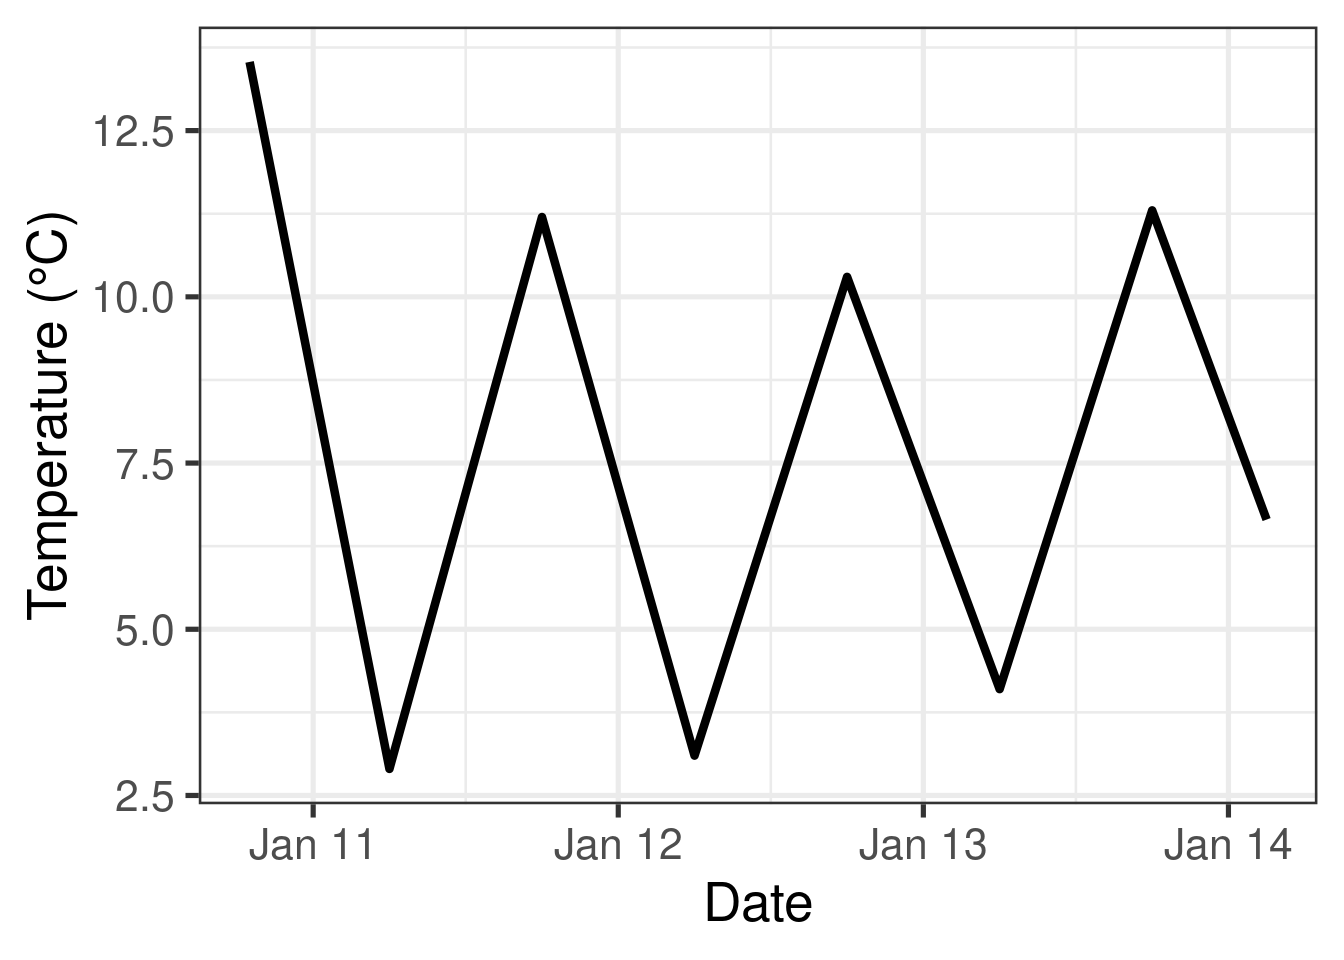
\includegraphics[width=0.8\linewidth,height=0.5\textheight]{Book_files/figure-latex/triangular-1}

This may not be a totally unreasonable approximation, but of course this isn't particularly realistic. The rate of temperature increase in the morning is not the same as the rate of decrease in the evening. Besides, in particular the time of the lowest daily temperature varies considerably throughout the year (unless you're close to the equator), and it would be good to consider this.

\hypertarget{idealized-daily-temperature-curves}{%
\subsection{Idealized daily temperature curves}\label{idealized-daily-temperature-curves}}

A major step forward was taken when Dale E. Linvill from Clemson University in South Carolina (USA) published a paper \href{https://journals.ashs.org/hortsci/view/journals/hortsci/25/1/article-p14.xml}{(Linvill \protect\hyperlink{ref-linvill1990calculating}{1990})} that described the daily temperature curve using a combination of two mathematical equations: a sine curve to describe daytime warming, and a logarithmic decay function for nighttime cooling. The transition points between the two parts were determined by sunrise and sunset, and the duration of the parts was related to daylength. The equations in this paper paved the way for making more realistic daily temperature curves than could easily be constructed before. This of course doesn't mean that all studies that came later used these equations - very far from it! This is mainly because people have either not been aware of these equations, or they were lacking the data processing skills to use them in their work.

One aspect that made Linvill's equations hard to use across different locations was the dependency on sunrise and sunset times. Of course, tables of these times can be produced from observations everywhere, but modelers would greatly benefit from a generic method to determine these. Fortunately, at least for locations without major topographic features, sunrise and sunset times can be calculated based on what we know about the geometry of our solar system. As agricultural scientists, this doesn't come naturally to us, but we can make use of what researchers in other fields have found out. The procedures in \texttt{chillR} rely on equations produced by \href{https://www.mail-archive.com/sundial@uni-koeln.de/msg01050.html}{(Spencer \protect\hyperlink{ref-spencer1971fourier}{1971})} and \href{https://www.sciencedirect.com/science/article/abs/pii/S0196890404001992}{(Almorox, Hontoria, and Benito \protect\hyperlink{ref-almorox2005statistical}{2005})}. Don't ask me now how exactly these equations work, since I don't remember\ldots{} It was enough to figure this out once, in the early days of my chilling analysis career, code it into an R function (or actually first a \texttt{JSL} function, but that's another story) and then just rely on that function for all subsequent work.

Putting together all these functions (\href{https://www.mail-archive.com/sundial@uni-koeln.de/msg01050.html}{(Spencer \protect\hyperlink{ref-spencer1971fourier}{1971})}, \href{https://www.sciencedirect.com/science/article/abs/pii/S0196890404001992}{(Almorox, Hontoria, and Benito \protect\hyperlink{ref-almorox2005statistical}{2005})} and \href{https://journals.ashs.org/hortsci/view/journals/hortsci/25/1/article-p14.xml}{(Linvill \protect\hyperlink{ref-linvill1990calculating}{1990})}) basically worked the same way as what we've just seen with the development of the \texttt{CH()} function and its subsequent embedding in the \texttt{sum\_CH} function - just that the individual components were a bit more complex. The result was a function that can produce credible daily temperature curves based only on the latitude of the location of interest.

The code below provides some use examples of the \texttt{daylength} function, which is involved in producing daily temperature curves. Let's make plots of the sunrise time, sunset time and daylength at Klein-Altendorf (Latitude: 50.4°N) over the course of the year.

\begin{Shaded}
\begin{Highlighting}[]
\KeywordTok{require}\NormalTok{(chillR)}
\KeywordTok{require}\NormalTok{(ggplot2)}
\KeywordTok{require}\NormalTok{(reshape2)}
\NormalTok{Days<-}\KeywordTok{daylength}\NormalTok{(}\DataTypeTok{latitude=}\FloatTok{50.4}\NormalTok{,}\DataTypeTok{JDay=}\DecValTok{1}\OperatorTok{:}\DecValTok{365}\NormalTok{)}
\NormalTok{Days_df<-}\KeywordTok{data.frame}\NormalTok{(}\DataTypeTok{JDay=}\DecValTok{1}\OperatorTok{:}\DecValTok{365}\NormalTok{,}\DataTypeTok{Sunrise=}\NormalTok{Days}\OperatorTok{$}\NormalTok{Sunrise,}\DataTypeTok{Sunset=}\NormalTok{Days}\OperatorTok{$}\NormalTok{Sunset,}\DataTypeTok{Daylength=}\NormalTok{Days}\OperatorTok{$}\NormalTok{Daylength)}
\NormalTok{Days_df<-}\KeywordTok{melt}\NormalTok{(Days_df, }\DataTypeTok{id=}\KeywordTok{c}\NormalTok{(}\StringTok{"JDay"}\NormalTok{)) }
\KeywordTok{ggplot}\NormalTok{(Days_df, }\KeywordTok{aes}\NormalTok{(JDay, value)) }\OperatorTok{+}\StringTok{ }\KeywordTok{geom_line}\NormalTok{(}\DataTypeTok{lwd=}\FloatTok{1.5}\NormalTok{) }\OperatorTok{+}\StringTok{ }\KeywordTok{facet_grid}\NormalTok{(}\DataTypeTok{cols=}\KeywordTok{vars}\NormalTok{(variable)) }\OperatorTok{+}
\StringTok{  }\KeywordTok{ylab}\NormalTok{(}\StringTok{"Time of Day / Daylength (Hours)"}\NormalTok{) }\OperatorTok{+}\StringTok{ }\KeywordTok{theme_bw}\NormalTok{(}\DataTypeTok{base_size =} \DecValTok{20}\NormalTok{)}
\end{Highlighting}
\end{Shaded}

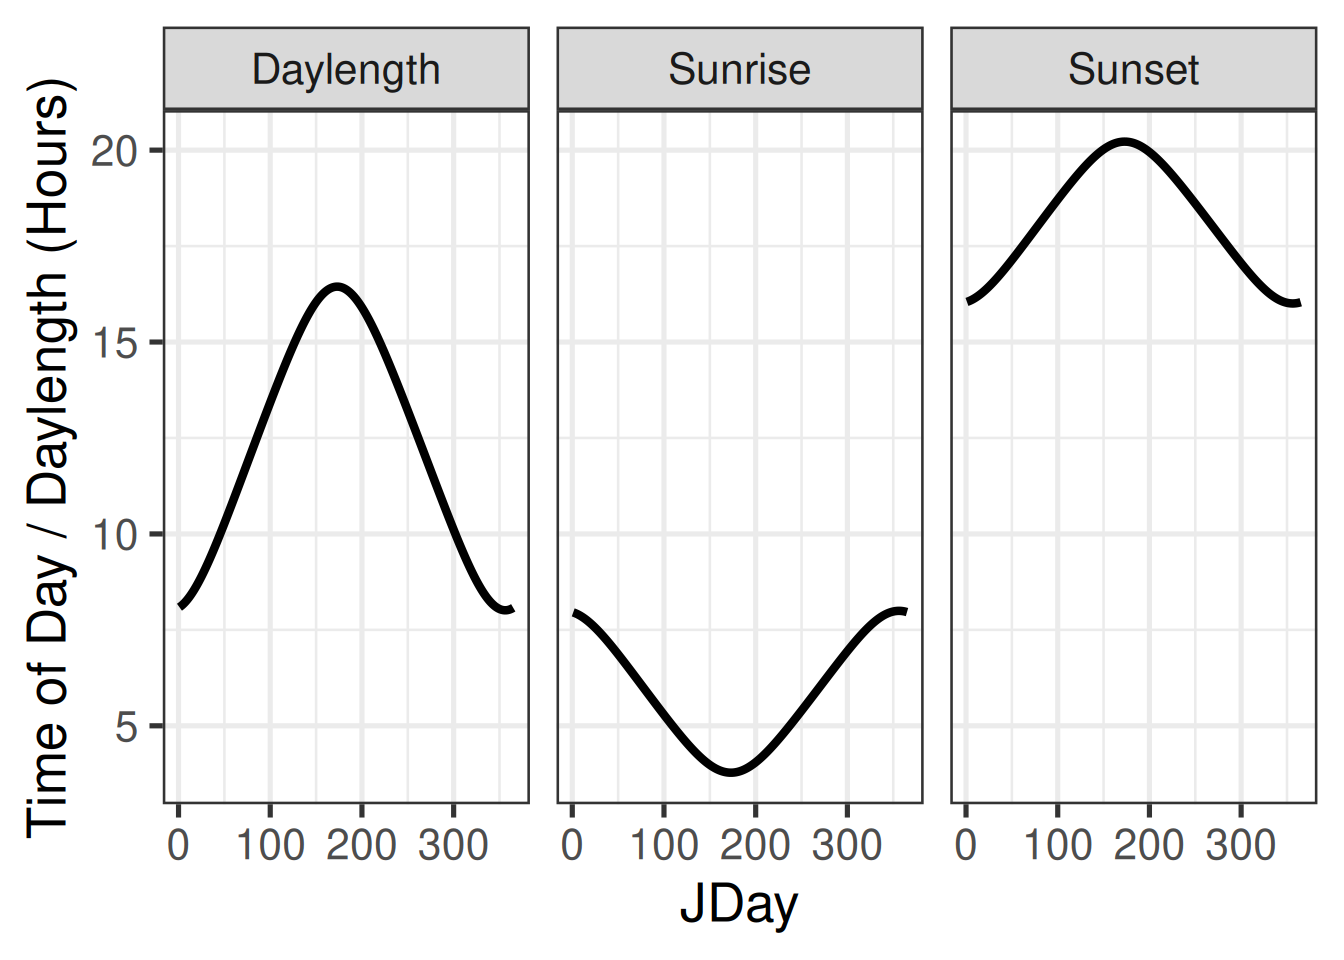
\includegraphics[width=0.8\linewidth,height=0.5\textheight]{Book_files/figure-latex/daily_curves-1}

Here, JDay is the so-called Julian Date, which basically means the Day of the Year. January 1\textsuperscript{st} ist JDay 1, and December 31\textsuperscript{st} either JDay 365 (in normal years) or JDay 366 (in leap years). I'm using the \href{https://ggplot2.tidyverse.org/}{\texttt{ggplot2}} package, which is a really elegant tool for making attractive plots. We'll get to talk a bit more about how this works. The ideal input for this is a data.frame, so I converted the outputs of the \texttt{daylength()} function into a data.frame first. I also had to convert the data.frame, so that the three time series (Sunrise, Sunset and Daylength) were stacked on top of each other. That was accomplished by the \texttt{melt} command of the \texttt{reshape2} package.

These daily dynamics are integrated in the \texttt{stack\_hourly\_temps()} function in \texttt{chillR}. This function takes as input a dataset of daily minimum and maximum temperatures (must have columns called \texttt{Tmin} and \texttt{Tmax}, as well as \texttt{Year}, \texttt{Month} and \texttt{Day}). It also needs to be told the latitude of the place of interest. With these inputs, we can apply the various equations we just discussed and calculate hourly temperatures. Optionally, we can also choose to output, in addition, the sunrise and sunset times.

To illustrate how this works, we'll use another dataset that comes with \texttt{chillR}: \texttt{KA\_weather}. This is a \texttt{data.frame} that contains temperature data for the experimental station of the University of Bonn at Klein-Altendorf. Here are the first 10 rows of the \texttt{KA\_weather} dataset:

\begingroup\fontsize{10}{12}\selectfont

\begin{tabular}{r|r|r|r|r}
\hline
Year & Month & Day & Tmax & Tmin\\
\hline
1998 & 1 & 1 & 8.2 & 5.1\\
\hline
1998 & 1 & 2 & 9.1 & 5.0\\
\hline
1998 & 1 & 3 & 10.4 & 3.3\\
\hline
1998 & 1 & 4 & 8.4 & 4.5\\
\hline
1998 & 1 & 5 & 7.7 & 4.5\\
\hline
1998 & 1 & 6 & 8.1 & 4.4\\
\hline
1998 & 1 & 7 & 12.0 & 6.9\\
\hline
1998 & 1 & 8 & 11.2 & 8.6\\
\hline
1998 & 1 & 9 & 13.9 & 8.5\\
\hline
1998 & 1 & 10 & 14.5 & 3.6\\
\hline
\end{tabular}
\endgroup{}

And this is how we can convert this to hourly temperatures based on the idealized curve:

\texttt{stack\_hourly\_temps(KA\_weather,\ latitude=50.4)}

\begingroup\fontsize{10}{12}\selectfont

\begin{tabular}{r|r|r|r|r|r|r|r}
\hline
Year & Month & Day & Tmax & Tmin & JDay & Hour & Temp\\
\hline
1998 & 1 & 5 & 7.7 & 4.5 & 5 & 3 & 4.854275\\
\hline
1998 & 1 & 5 & 7.7 & 4.5 & 5 & 4 & 4.757002\\
\hline
1998 & 1 & 5 & 7.7 & 4.5 & 5 & 5 & 4.666981\\
\hline
1998 & 1 & 5 & 7.7 & 4.5 & 5 & 6 & 4.583205\\
\hline
1998 & 1 & 5 & 7.7 & 4.5 & 5 & 7 & 4.504863\\
\hline
1998 & 1 & 5 & 7.7 & 4.5 & 5 & 8 & 4.568913\\
\hline
1998 & 1 & 5 & 7.7 & 4.5 & 5 & 9 & 5.383559\\
\hline
1998 & 1 & 5 & 7.7 & 4.5 & 5 & 10 & 6.139624\\
\hline
1998 & 1 & 5 & 7.7 & 4.5 & 5 & 11 & 6.786976\\
\hline
1998 & 1 & 5 & 7.7 & 4.5 & 5 & 12 & 7.282696\\
\hline
1998 & 1 & 5 & 7.7 & 4.5 & 5 & 13 & 7.593916\\
\hline
1998 & 1 & 5 & 7.7 & 4.5 & 5 & 14 & 7.700000\\
\hline
1998 & 1 & 5 & 7.7 & 4.5 & 5 & 15 & 7.593916\\
\hline
1998 & 1 & 5 & 7.7 & 4.5 & 5 & 16 & 7.282696\\
\hline
1998 & 1 & 5 & 7.7 & 4.5 & 5 & 17 & 6.591632\\
\hline
1998 & 1 & 5 & 7.7 & 4.5 & 5 & 18 & 6.167994\\
\hline
1998 & 1 & 5 & 7.7 & 4.5 & 5 & 19 & 5.870540\\
\hline
1998 & 1 & 5 & 7.7 & 4.5 & 5 & 20 & 5.641103\\
\hline
1998 & 1 & 5 & 7.7 & 4.5 & 5 & 21 & 5.454295\\
\hline
1998 & 1 & 5 & 7.7 & 4.5 & 5 & 22 & 5.296730\\
\hline
1998 & 1 & 5 & 7.7 & 4.5 & 5 & 23 & 5.160480\\
\hline
\end{tabular}
\endgroup{}

And here's a plot of the data:

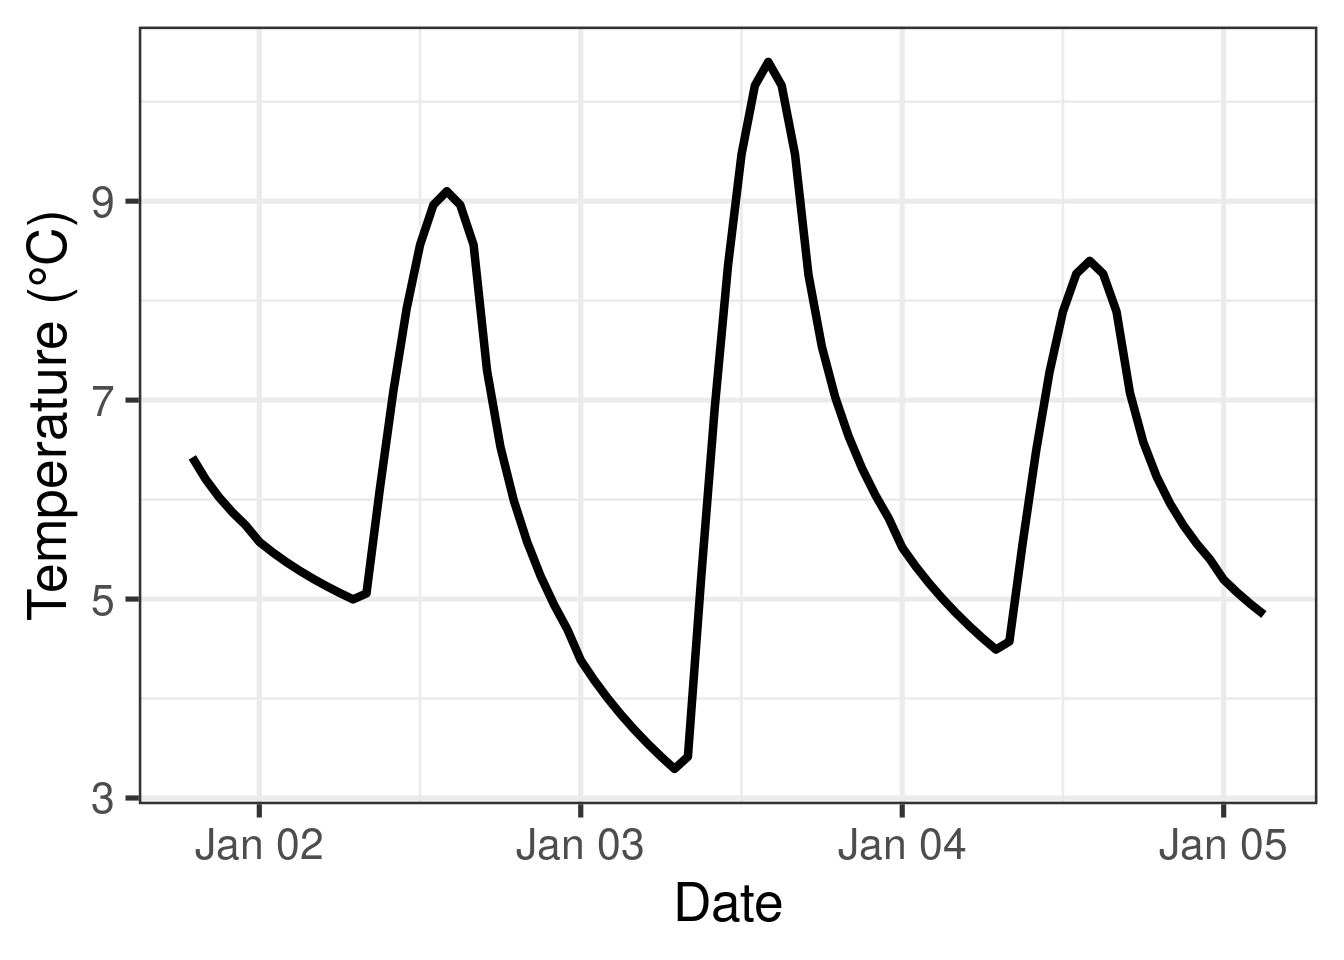
\includegraphics[width=0.8\linewidth,height=0.5\textheight]{Book_files/figure-latex/idealized-1}

\hypertarget{empirical-daily-temperature-curves}{%
\subsection{Empirical daily temperature curves}\label{empirical-daily-temperature-curves}}

There are some locations where idealized daily temperature curves don't work. For instance, some places where temperate fruit trees are grown feature rugged topography, so that trees may be shaded for part of the day. The pictures below show the region where I first started working on winter chill - the Jabal Al Akhdar (the Green Mountain) region in Oman. We investigated several oases in Wadi Muaydin, a deeply incised canyon. Near the top of the canyon, trees get a lot more sunlight than at the bottom of the valley, more than 1000 m below.

\begin{figure}
\centering
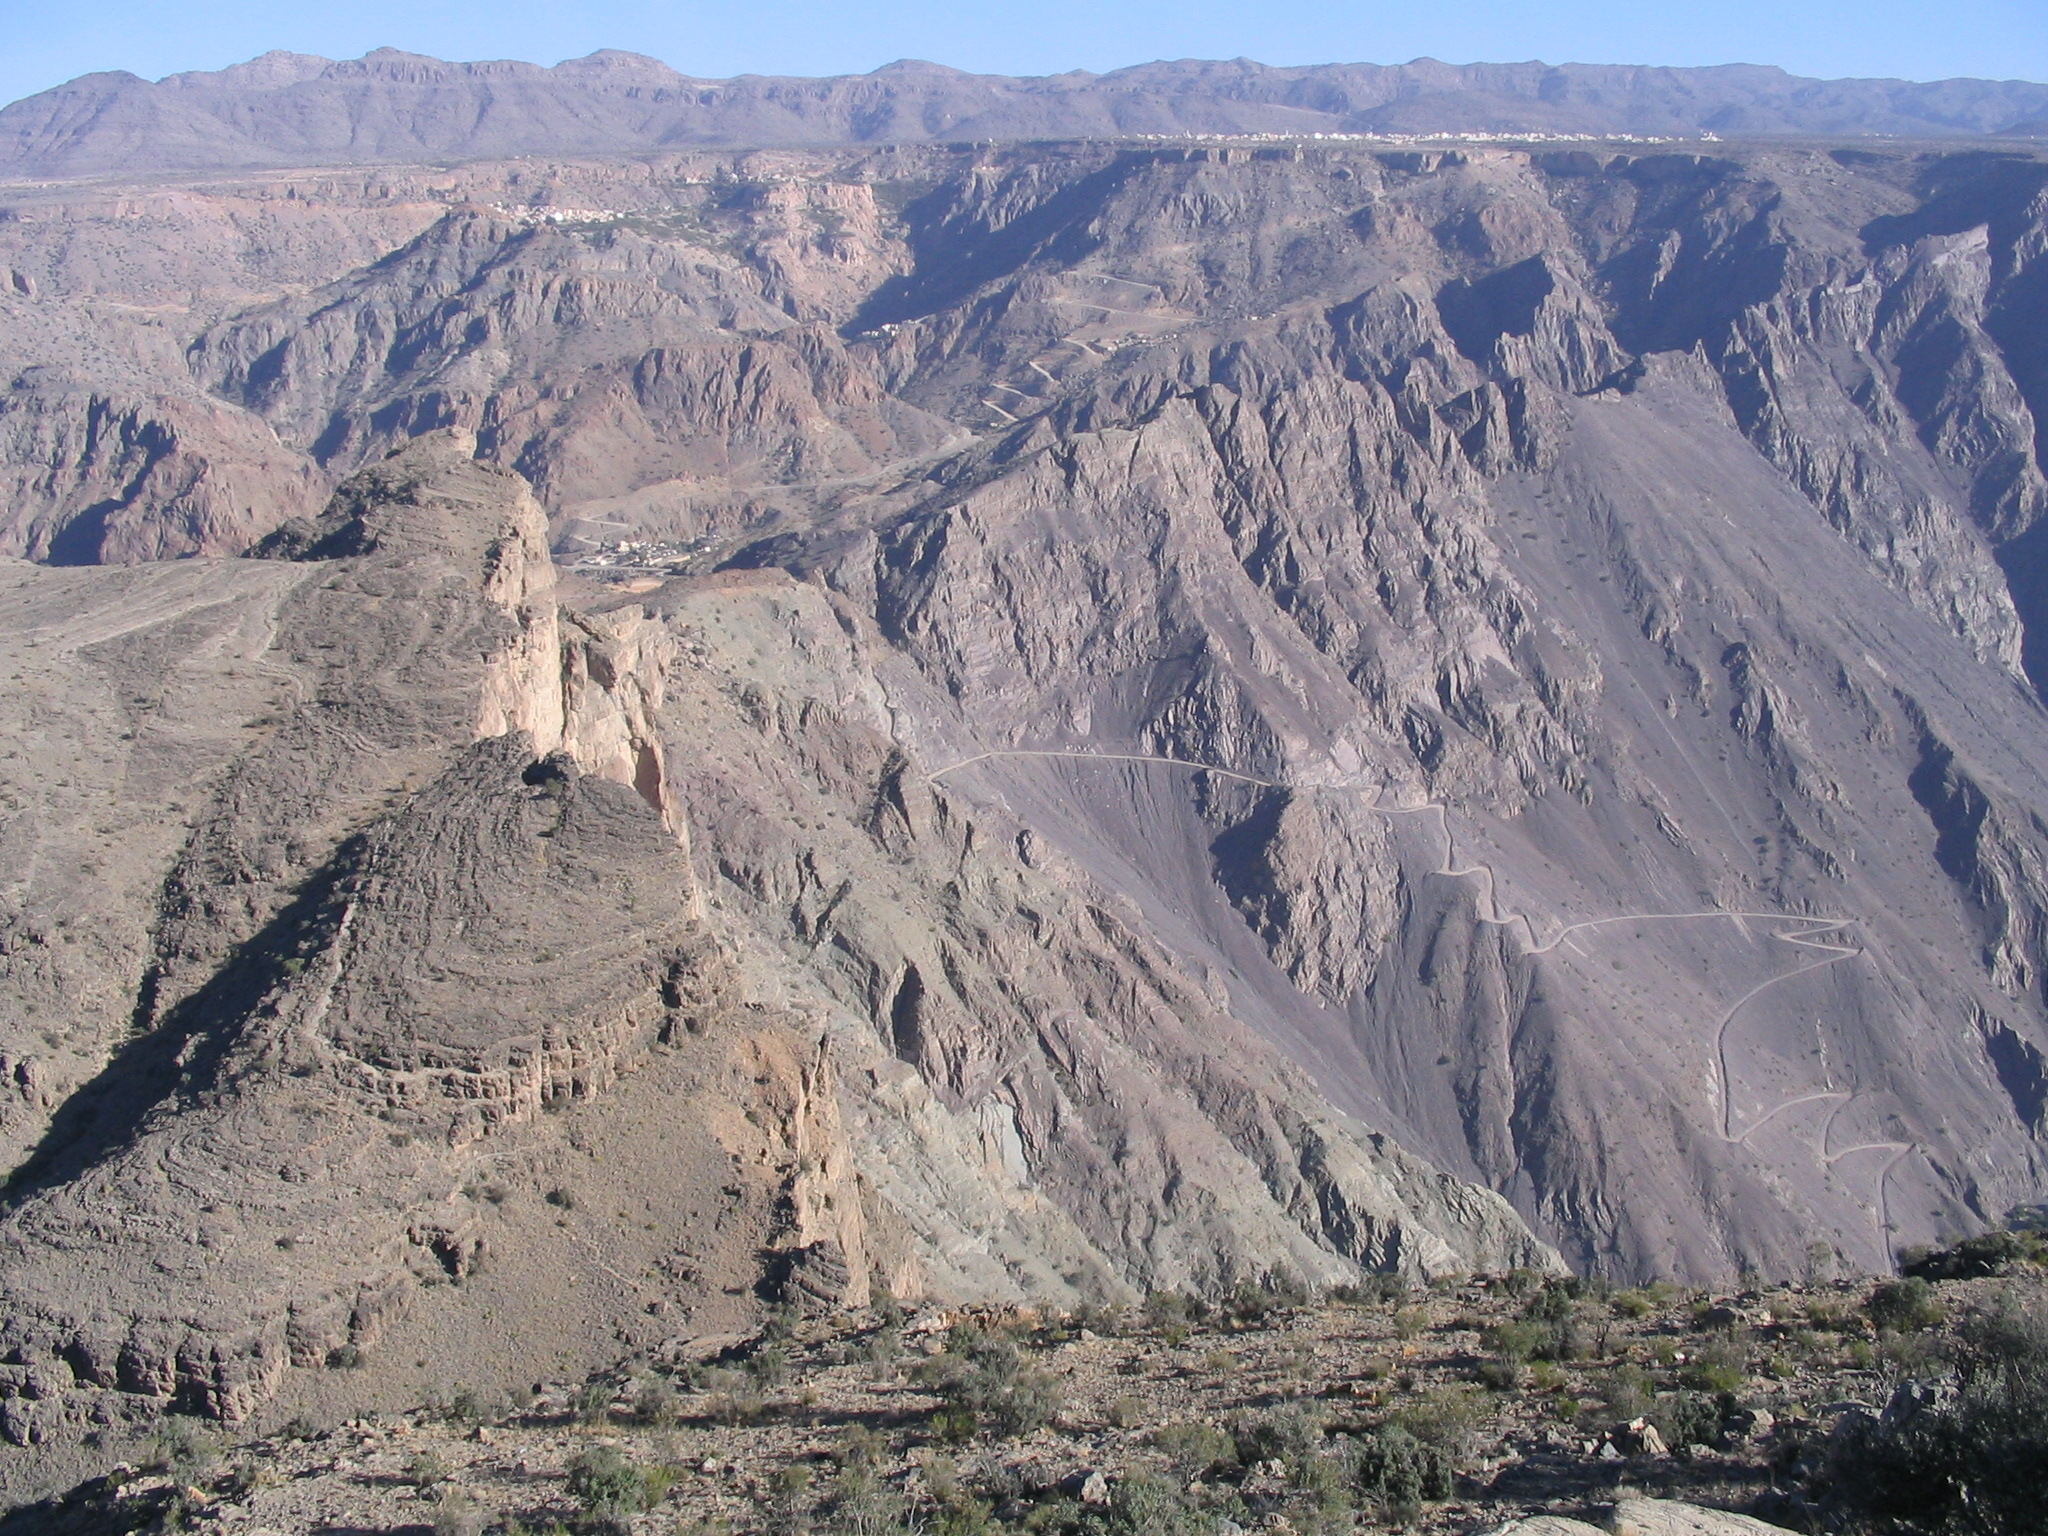
\includegraphics[width=0.9\textwidth,height=\textheight]{pictures/IMG_5403.JPG}
\caption{Overview of Wadi Muaydin - the lowest oasis, Masayrat ar Ruwajah, is at the end of the steep, curvy road you can see disappear at the bottom of the image.}
\end{figure}

\begin{figure}
\centering
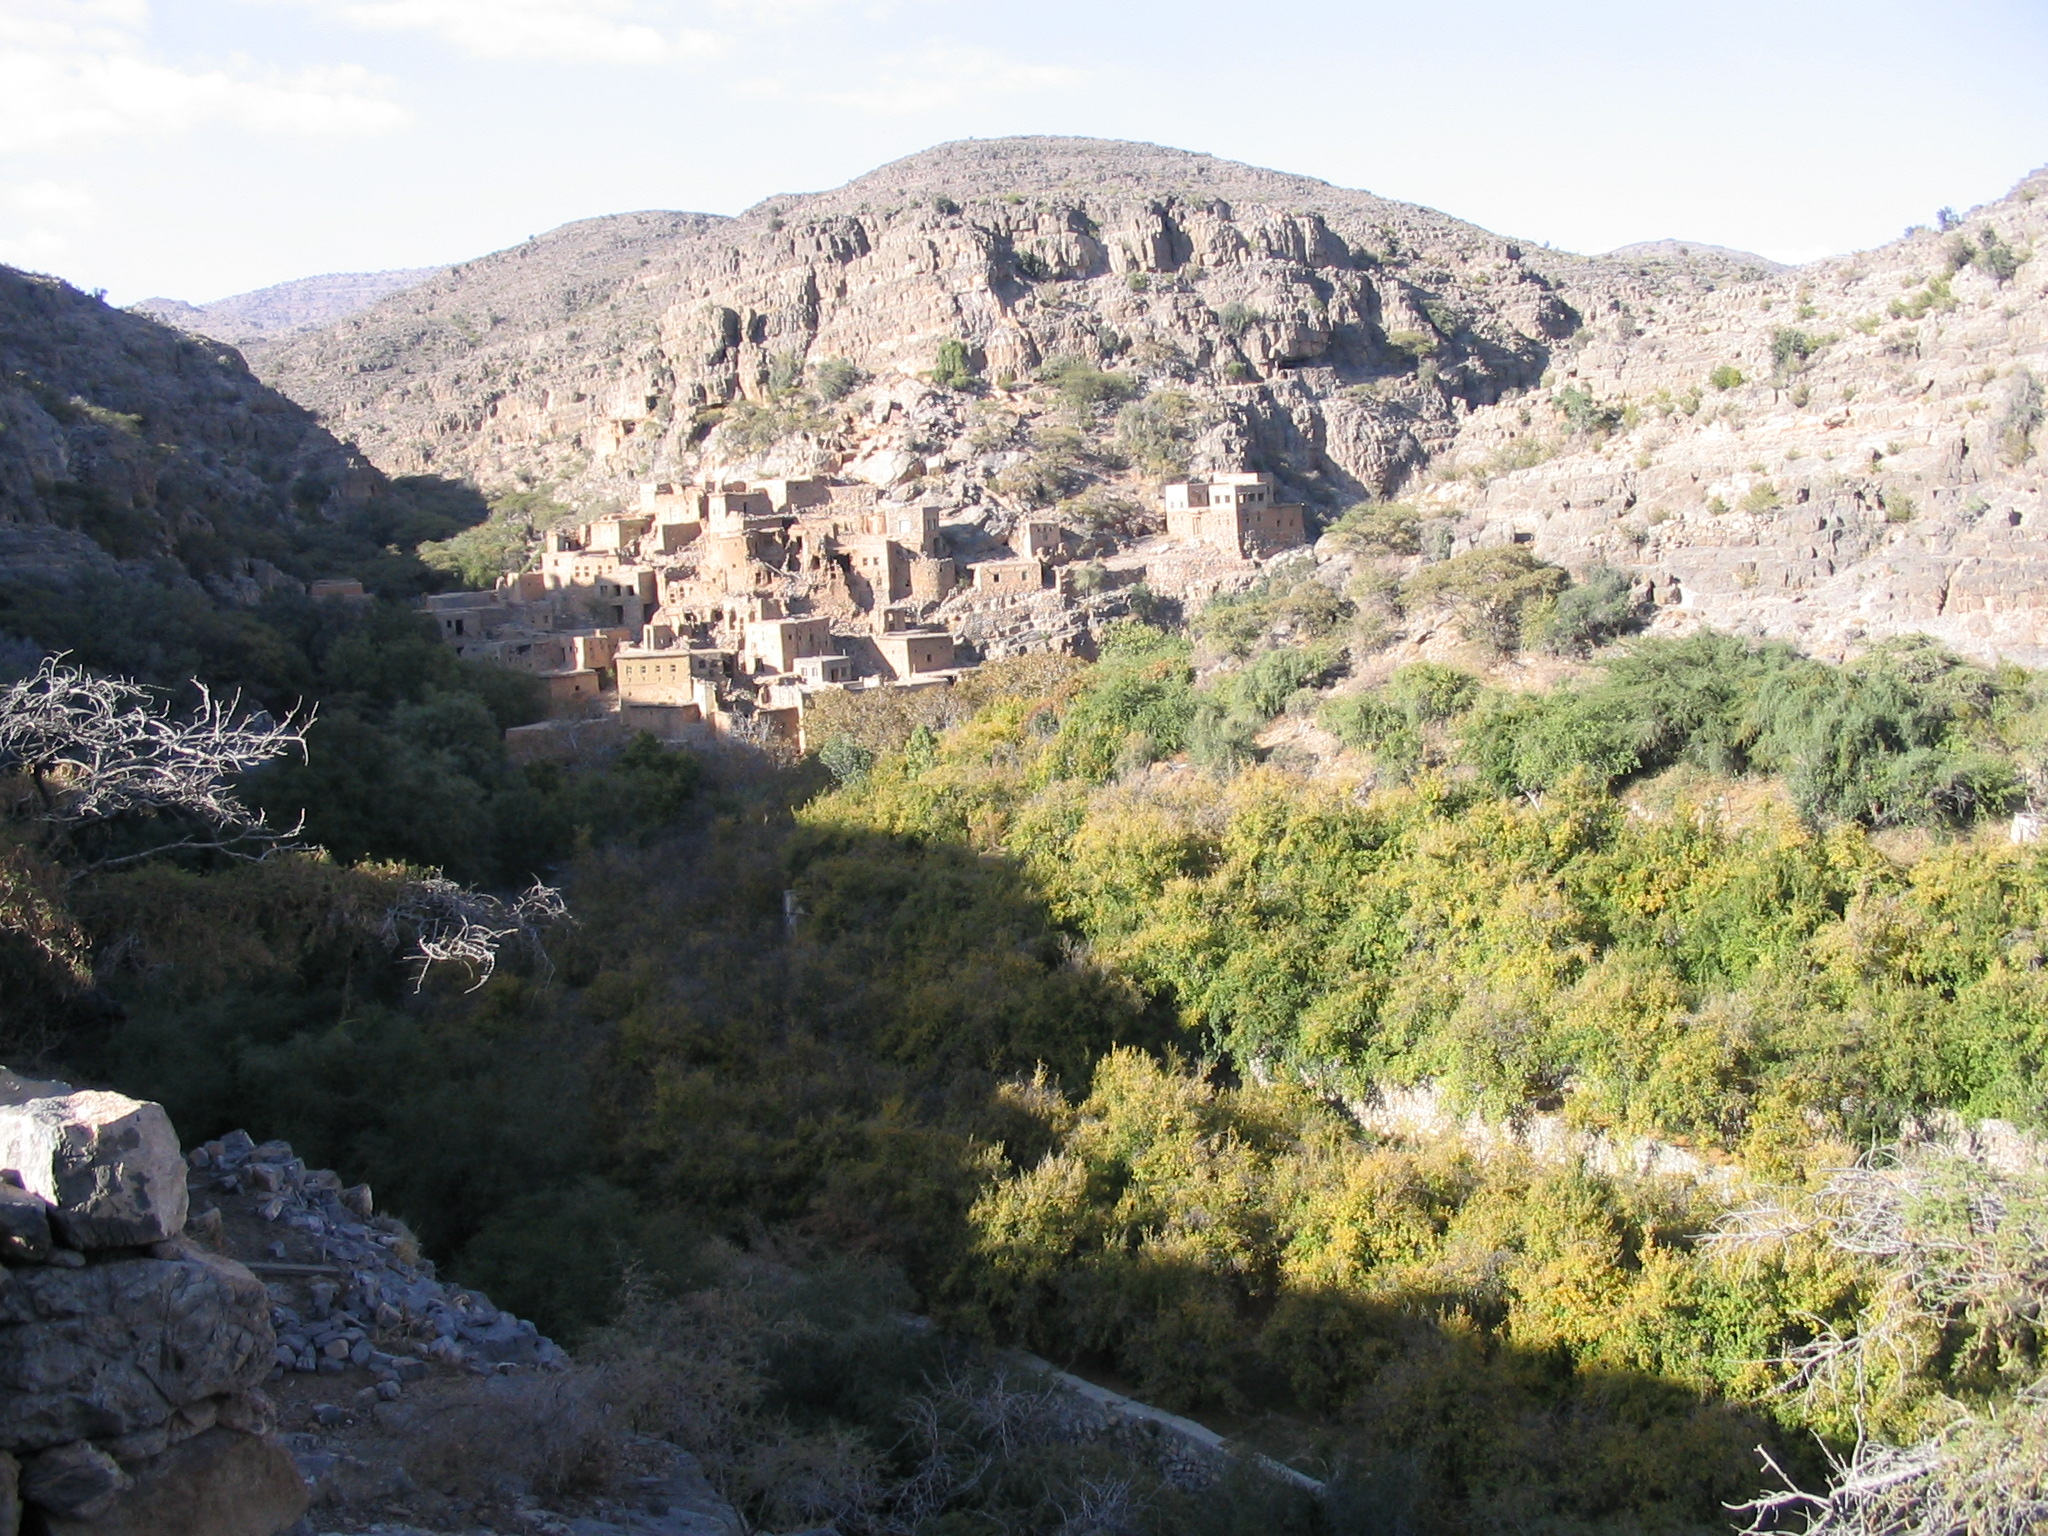
\includegraphics[width=0.9\textwidth,height=\textheight]{pictures/IMG_5573.JPG}
\caption{Impression of the oasis of Wadi Bani Habib (a few kilometers away) illustrating the impact that toppgraphic shading can have.}
\end{figure}

\begin{figure}
\centering
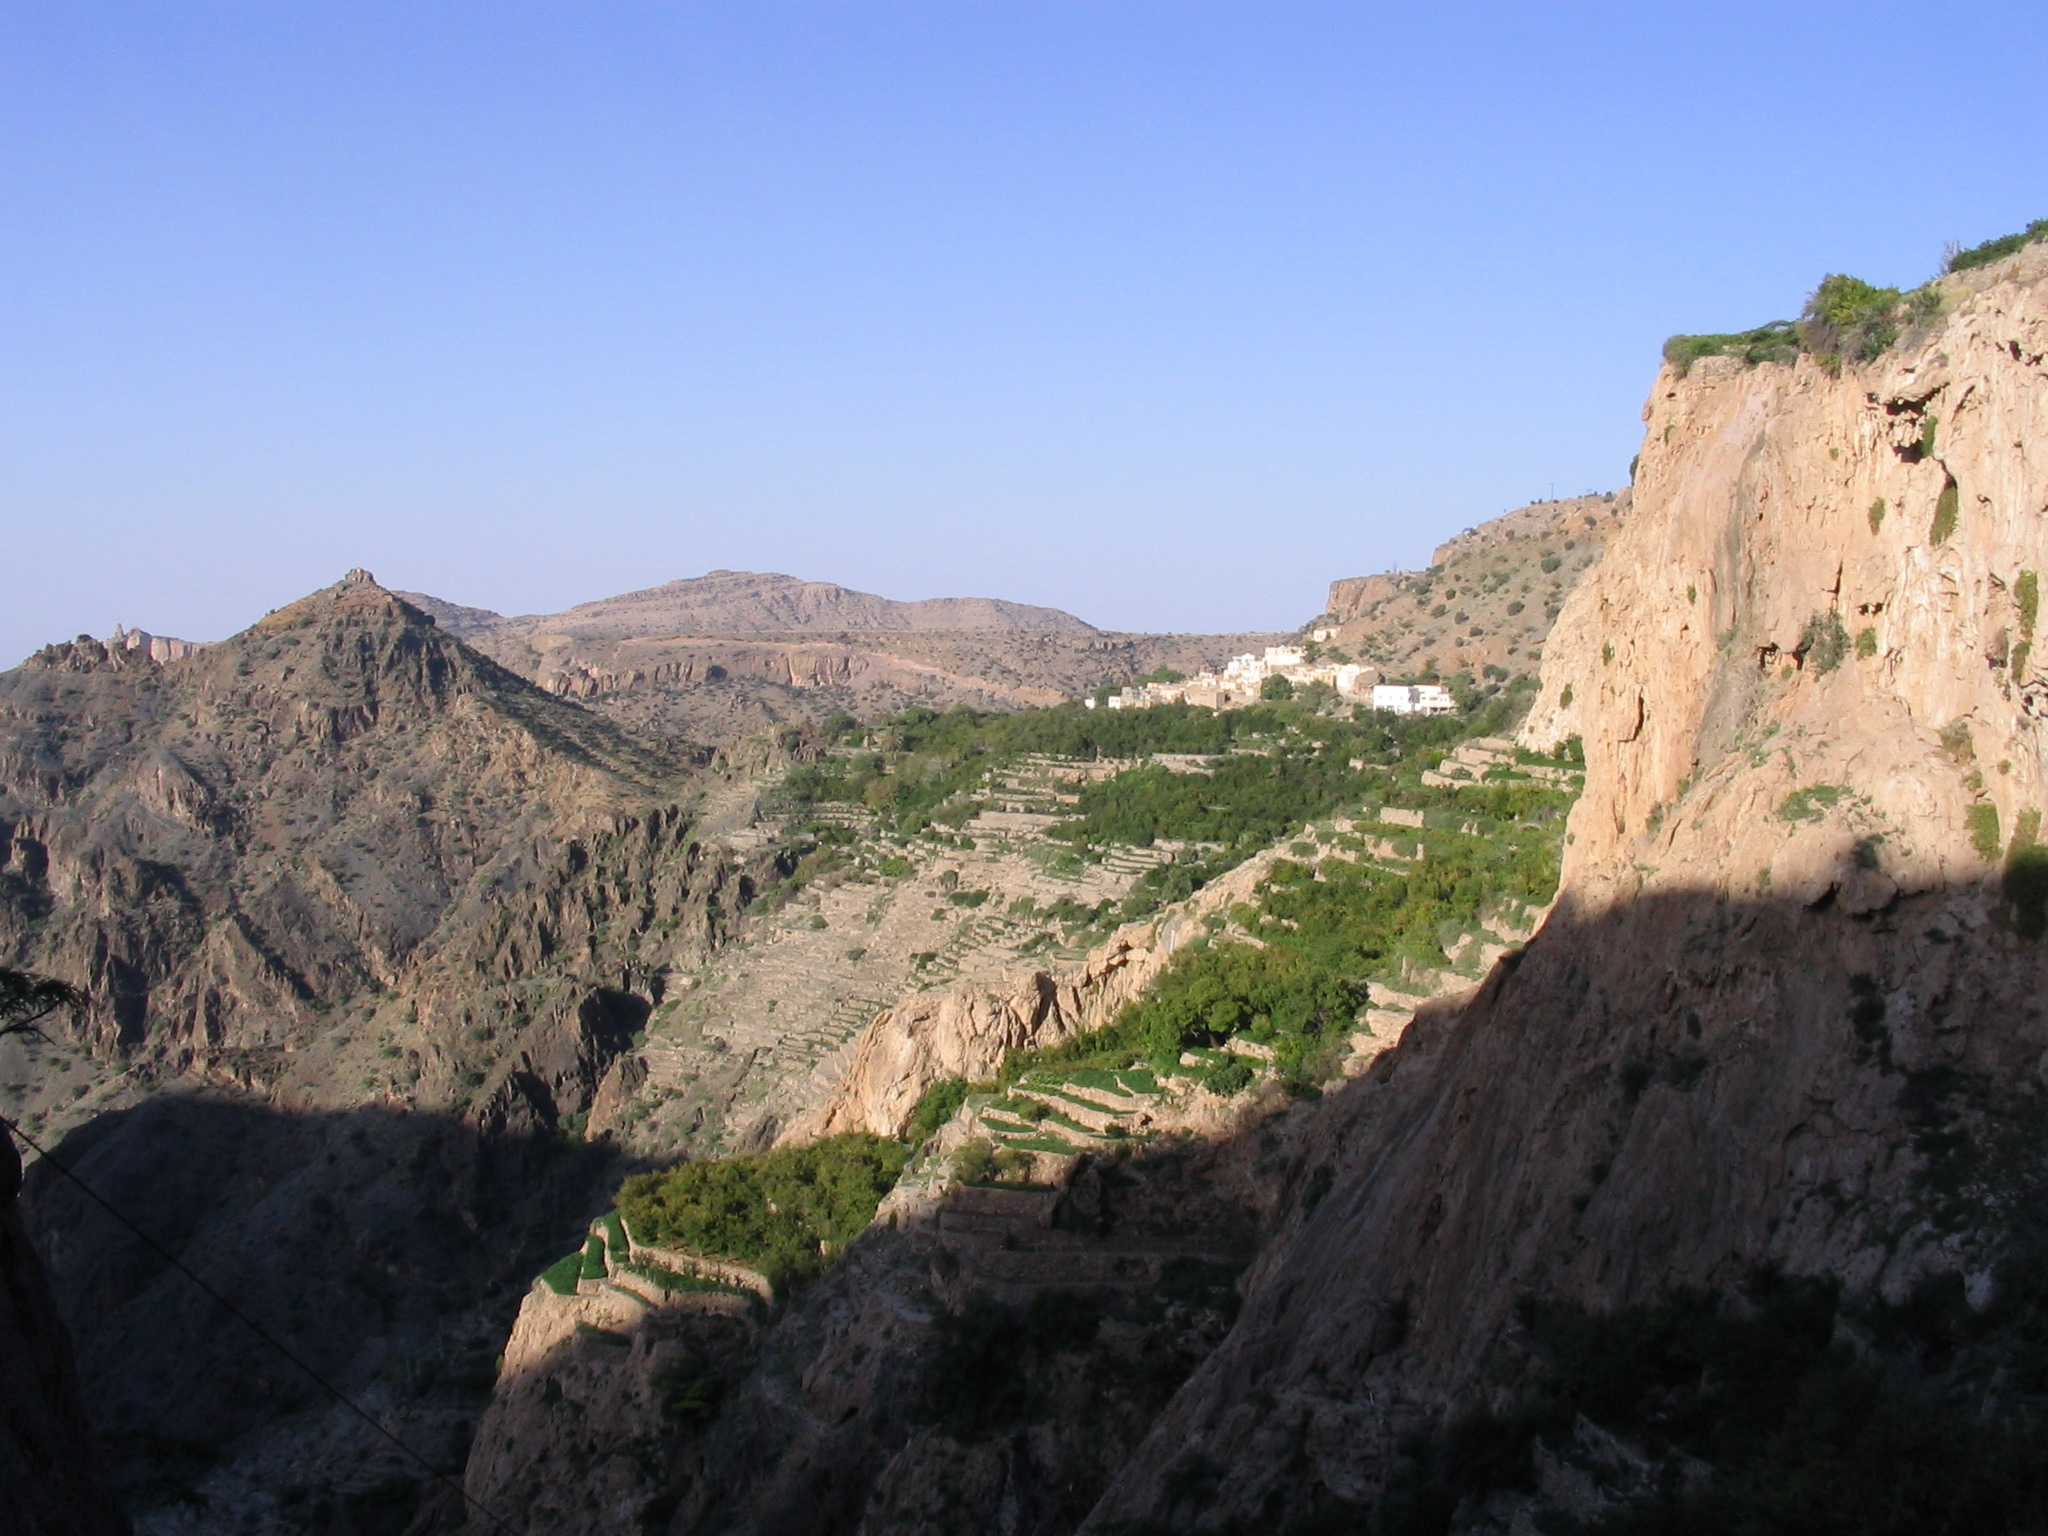
\includegraphics[width=0.9\textwidth,height=\textheight]{pictures/IMG_8487.JPG}
\caption{Terraced oasis fields at Ash Sharayjah. The pomegranates and other temperate tree crops there are already enjoying the morning sun. Trees in the oasis of Qasha', located in the lower left corner of the image, are still hidden in the shadows.}
\end{figure}

Even without such mountains, it seems quite likely that the temperature curve in an orchard, which may feature its own microclimate, with shaded and sunny spots, with dew-covered grass or bare ground etc., may not closely resemble the curve drawn up by Linvill \href{https://journals.ashs.org/hortsci/view/journals/hortsci/25/1/article-p14.xml}{(Linvill \protect\hyperlink{ref-linvill1990calculating}{1990})}.

In our first study on the Omani oases \href{https://link.springer.com/article/10.1007/s10584-009-9581-7}{(Luedeling, Gebauer, and Buerkert \protect\hyperlink{ref-luedeling_climate_2009}{2009})}, we didn't address this issue very well (not even with the idealized daily curve yet), but we recently revisited this location, this time committed to doing this better. Here's what we came up with \href{https://link.springer.com/article/10.1007/s10584-020-02862-8}{(Buerkert et al. \protect\hyperlink{ref-buerkert2020revisiting}{2020})}:

\begin{enumerate}
\def\labelenumi{\arabic{enumi})}
\item
  First we need a dataset of hourly temperature data for the location of interest. This should cover a full year, and ideally multiple years. For the purpose of this exercise, we'll use the \texttt{Winters\_hours\_gaps} dataset, which is included in \texttt{chillR}. I collected this dataset in a walnut orchard near Winters, California. The temperature logger was attached directly to a tree branch, so I wouldn't expect the data to precisely mirror the usual daily temperature curve.
\item
  We now use the \texttt{Empirical\_daily\_temperature\_curve()} function to determine the typical pattern of hourly temperatures at this location. This is done separately for each month of the year (there may still be room for improvement here - this could be continuous and not broken down by months).
\end{enumerate}

\begin{Shaded}
\begin{Highlighting}[]
\NormalTok{empi_curve<-}\KeywordTok{Empirical_daily_temperature_curve}\NormalTok{(Winters_hours_gaps)}
\end{Highlighting}
\end{Shaded}

Let's see what the results look like, in a table and a figure.

\begin{Shaded}
\begin{Highlighting}[]
\KeywordTok{kable}\NormalTok{(empi_curve[}\DecValTok{1}\OperatorTok{:}\DecValTok{48}\NormalTok{,])  }\OperatorTok
\StringTok{  }\KeywordTok{kable_styling}\NormalTok{(}\StringTok{"striped"}\NormalTok{, }\DataTypeTok{position =} \StringTok{"left"}\NormalTok{,}\DataTypeTok{font_size =} \DecValTok{10}\NormalTok{)}
\end{Highlighting}
\end{Shaded}

\begingroup\fontsize{10}{12}\selectfont

\begin{tabular}{r|r|r}
\hline
Month & Hour & Prediction\_coefficient\\
\hline
3 & 0 & 0.1774859\\
\hline
3 & 1 & 0.1550693\\
\hline
3 & 2 & 0.1285651\\
\hline
3 & 3 & 0.1145597\\
\hline
3 & 4 & 0.0696064\\
\hline
3 & 5 & 0.0339583\\
\hline
3 & 6 & 0.0000000\\
\hline
3 & 7 & 0.0313115\\
\hline
3 & 8 & 0.3121959\\
\hline
3 & 9 & 0.4953232\\
\hline
3 & 10 & 0.6819674\\
\hline
3 & 11 & 0.8227423\\
\hline
3 & 12 & 0.9506491\\
\hline
3 & 13 & 0.9662604\\
\hline
3 & 14 & 0.9915996\\
\hline
3 & 15 & 1.0000000\\
\hline
3 & 16 & 0.9490319\\
\hline
3 & 17 & 0.8483098\\
\hline
3 & 18 & 0.6864529\\
\hline
3 & 19 & 0.4945415\\
\hline
3 & 20 & 0.3636642\\
\hline
3 & 21 & 0.2972377\\
\hline
3 & 22 & 0.2360349\\
\hline
3 & 23 & 0.1794802\\
\hline
4 & 0 & 0.1960789\\
\hline
4 & 1 & 0.1407018\\
\hline
4 & 2 & 0.1283250\\
\hline
4 & 3 & 0.0819307\\
\hline
4 & 4 & 0.0541415\\
\hline
4 & 5 & 0.0188241\\
\hline
4 & 6 & 0.0000000\\
\hline
4 & 7 & 0.1697052\\
\hline
4 & 8 & 0.4442722\\
\hline
4 & 9 & 0.5939797\\
\hline
4 & 10 & 0.7363923\\
\hline
4 & 11 & 0.8399804\\
\hline
4 & 12 & 0.9245702\\
\hline
4 & 13 & 0.9770693\\
\hline
4 & 14 & 0.9963131\\
\hline
4 & 15 & 1.0000000\\
\hline
4 & 16 & 0.9568107\\
\hline
4 & 17 & 0.8698369\\
\hline
4 & 18 & 0.7343896\\
\hline
4 & 19 & 0.5330597\\
\hline
4 & 20 & 0.3941038\\
\hline
4 & 21 & 0.3186075\\
\hline
4 & 22 & 0.2594569\\
\hline
4 & 23 & 0.2114486\\
\hline
\end{tabular}
\endgroup{}

\begin{Shaded}
\begin{Highlighting}[]
\KeywordTok{ggplot}\NormalTok{(}\DataTypeTok{data=}\NormalTok{empi_curve[}\DecValTok{1}\OperatorTok{:}\DecValTok{96}\NormalTok{,], }\KeywordTok{aes}\NormalTok{(Hour,Prediction_coefficient))}\OperatorTok{+}\KeywordTok{geom_line}\NormalTok{(}\DataTypeTok{lwd=}\FloatTok{1.3}\NormalTok{, }\DataTypeTok{col=}\StringTok{"red"}\NormalTok{)}\OperatorTok{+}\KeywordTok{facet_grid}\NormalTok{(}\DataTypeTok{rows=}\KeywordTok{vars}\NormalTok{(Month))}\OperatorTok{+}\KeywordTok{xlab}\NormalTok{(}\StringTok{"Hour of the day"}\NormalTok{)}\OperatorTok{+}\KeywordTok{ylab}\NormalTok{(}\StringTok{"Prediction coefficient"}\NormalTok{) }\OperatorTok{+}\StringTok{ }\KeywordTok{theme_bw}\NormalTok{(}\DataTypeTok{base_size=}\DecValTok{20}\NormalTok{)}
\end{Highlighting}
\end{Shaded}

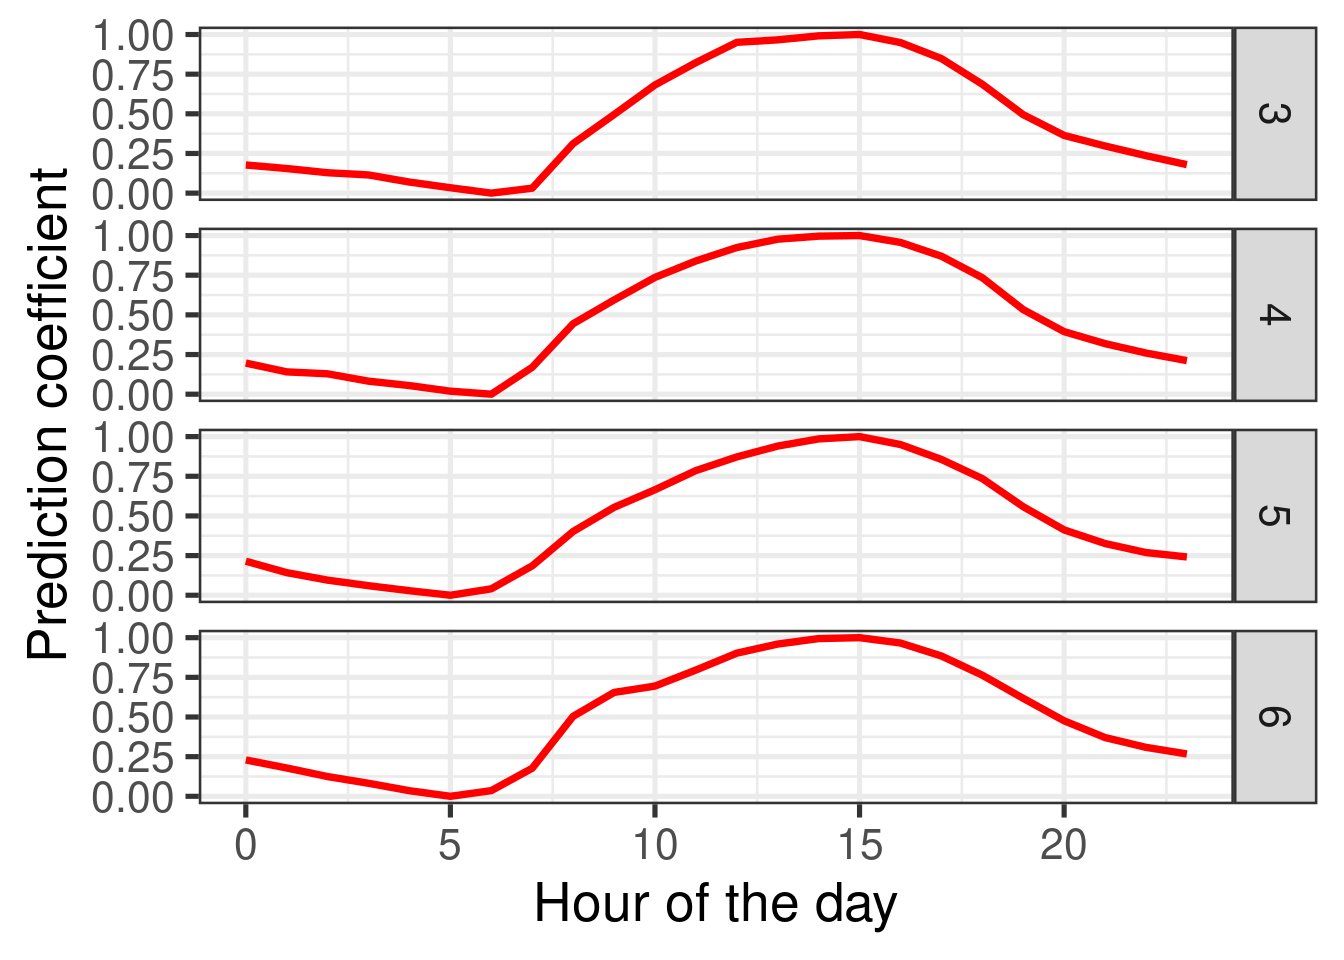
\includegraphics{Book_files/figure-latex/empirical_temperatures_output-1.pdf}

\begin{enumerate}
\def\labelenumi{\arabic{enumi})}
\setcounter{enumi}{2}
\tightlist
\item
  We can now apply this set of coefficients to a daily dataset from the same location, which should give us a reasonable hourly temperature record for this orchard. For this, we can use the \texttt{Empirical\_hourly\_temperatures} function, which requires as inputs a set of hourly coefficients (such as the one we just made), and a daily temperature record (which includes \texttt{Tmin} and \texttt{Tmax} columns). Did I mention that you can always use the \texttt{?} to get help on how to use a function (e.g.~\texttt{?Empirical\_hourly\_temperatures}).
\end{enumerate}

So here's how this works. Note that this also demonstrates use of the \texttt{make\_all\_day\_table} function, which can fill gaps in daily or hourly temperature records and - as in this case - summarize hourly records into daily minimum and maximum temperatures:

\begin{Shaded}
\begin{Highlighting}[]
\NormalTok{coeffs<-}\KeywordTok{Empirical_daily_temperature_curve}\NormalTok{(Winters_hours_gaps)}
\NormalTok{Winters_daily<-}\KeywordTok{make_all_day_table}\NormalTok{(Winters_hours_gaps, }\DataTypeTok{input_timestep=}\StringTok{"hour"}\NormalTok{)}
\NormalTok{Winters_hours<-}\KeywordTok{Empirical_hourly_temperatures}\NormalTok{(Winters_daily,coeffs)}
\end{Highlighting}
\end{Shaded}

This is it really. Let's plot the result to see what it looks like. We can also compare the results to those of the triangular function and the idealized temperature curve. In this example, we also have the actual observed temperatures, so we can use these to validate the results as well.

First, let's simplify the data a bit, so that it gets easier to use:

\begin{Shaded}
\begin{Highlighting}[]
\KeywordTok{require}\NormalTok{(reshape2)}

\NormalTok{Winters_hours<-Winters_hours[,}\KeywordTok{c}\NormalTok{(}\StringTok{"Year"}\NormalTok{,}\StringTok{"Month"}\NormalTok{,}\StringTok{"Day"}\NormalTok{,}\StringTok{"Hour"}\NormalTok{,}\StringTok{"Temp"}\NormalTok{)]}
\KeywordTok{colnames}\NormalTok{(Winters_hours)[}\KeywordTok{ncol}\NormalTok{(Winters_hours)]<-}\StringTok{"Temp_empirical"}
\NormalTok{Winters_ideal<-}\KeywordTok{stack_hourly_temps}\NormalTok{(Winters_daily, }\DataTypeTok{latitude=}\FloatTok{38.5}\NormalTok{)}\OperatorTok{$}\NormalTok{hourtemps}
\NormalTok{Winters_ideal<-Winters_ideal[,}\KeywordTok{c}\NormalTok{(}\StringTok{"Year"}\NormalTok{,}\StringTok{"Month"}\NormalTok{,}\StringTok{"Day"}\NormalTok{,}\StringTok{"Hour"}\NormalTok{,}\StringTok{"Temp"}\NormalTok{)]}
\KeywordTok{colnames}\NormalTok{(Winters_ideal)[}\KeywordTok{ncol}\NormalTok{(Winters_ideal)]<-}\StringTok{"Temp_ideal"}
\end{Highlighting}
\end{Shaded}

Now we make the `triangular' dataset. See if you can understand how this works.

\begin{Shaded}
\begin{Highlighting}[]
\NormalTok{Winters_triangle<-Winters_daily}
\NormalTok{Winters_triangle[,}\StringTok{"Hour"}\NormalTok{]<-}\DecValTok{0}
\NormalTok{Winters_triangle}\OperatorTok{$}\NormalTok{Hour[}\KeywordTok{nrow}\NormalTok{(Winters_triangle)]<-}\DecValTok{23}
\NormalTok{Winters_triangle[,}\StringTok{"Temp"}\NormalTok{]<-}\DecValTok{0}
\NormalTok{Winters_triangle<-}\KeywordTok{make_all_day_table}\NormalTok{(Winters_triangle,}\DataTypeTok{timestep=}\StringTok{"hour"}\NormalTok{)}
\KeywordTok{colnames}\NormalTok{(Winters_triangle)[}\KeywordTok{ncol}\NormalTok{(Winters_triangle)]<-}\StringTok{"Temp_triangular"}

\ControlFlowTok{for}\NormalTok{(i }\ControlFlowTok{in} \DecValTok{2}\OperatorTok{:}\KeywordTok{nrow}\NormalTok{(Winters_triangle))}
\NormalTok{\{}\ControlFlowTok{if}\NormalTok{(}\KeywordTok{is.na}\NormalTok{(Winters_triangle}\OperatorTok{$}\NormalTok{Tmin[i])) Winters_triangle}\OperatorTok{$}\NormalTok{Tmin[i]<-Winters_triangle}\OperatorTok{$}\NormalTok{Tmin[i}\DecValTok{-1}\NormalTok{]}
\ControlFlowTok{if}\NormalTok{(}\KeywordTok{is.na}\NormalTok{(Winters_triangle}\OperatorTok{$}\NormalTok{Tmax[i])) Winters_triangle}\OperatorTok{$}\NormalTok{Tmax[i]<-Winters_triangle}\OperatorTok{$}\NormalTok{Tmax[i}\DecValTok{-1}\NormalTok{]}
\NormalTok{\}}
\NormalTok{Winters_triangle}\OperatorTok{$}\NormalTok{Temp_triangular<-}\OtherTok{NA}

\NormalTok{Winters_triangle}\OperatorTok{$}\NormalTok{Temp_triangular[}\KeywordTok{which}\NormalTok{(Winters_triangle}\OperatorTok{$}\NormalTok{Hour}\OperatorTok{==}\DecValTok{6}\NormalTok{)]<-}
\StringTok{  }\NormalTok{Winters_triangle}\OperatorTok{$}\NormalTok{Tmin[}\KeywordTok{which}\NormalTok{(Winters_triangle}\OperatorTok{$}\NormalTok{Hour}\OperatorTok{==}\DecValTok{6}\NormalTok{)] }
\NormalTok{Winters_triangle}\OperatorTok{$}\NormalTok{Temp_triangular[}\KeywordTok{which}\NormalTok{(Winters_triangle}\OperatorTok{$}\NormalTok{Hour}\OperatorTok{==}\DecValTok{18}\NormalTok{)]<-}
\StringTok{  }\NormalTok{Winters_triangle}\OperatorTok{$}\NormalTok{Tmax[}\KeywordTok{which}\NormalTok{(Winters_triangle}\OperatorTok{$}\NormalTok{Hour}\OperatorTok{==}\DecValTok{18}\NormalTok{)] }
\NormalTok{Winters_triangle}\OperatorTok{$}\NormalTok{Temp_triangular<-}
\StringTok{  }\KeywordTok{interpolate_gaps}\NormalTok{(Winters_triangle}\OperatorTok{$}\NormalTok{Temp_triangular)}\OperatorTok{$}\NormalTok{interp}
\NormalTok{Winters_triangle<-Winters_triangle[,}\KeywordTok{c}\NormalTok{(}\StringTok{"Year"}\NormalTok{,}\StringTok{"Month"}\NormalTok{,}\StringTok{"Day"}\NormalTok{,}\StringTok{"Hour"}\NormalTok{,}\StringTok{"Temp_triangular"}\NormalTok{)]}
\end{Highlighting}
\end{Shaded}

Now we merge all these \texttt{data.frames} so that we can easily display them:

\begin{Shaded}
\begin{Highlighting}[]
\NormalTok{Winters_temps<-}\KeywordTok{merge}\NormalTok{(Winters_hours_gaps,Winters_hours, }\DataTypeTok{by=}\KeywordTok{c}\NormalTok{(}\StringTok{"Year"}\NormalTok{,}\StringTok{"Month"}\NormalTok{,}\StringTok{"Day"}\NormalTok{,}\StringTok{"Hour"}\NormalTok{))}
\NormalTok{Winters_temps<-}\KeywordTok{merge}\NormalTok{(Winters_temps,Winters_triangle, }\DataTypeTok{by=}\KeywordTok{c}\NormalTok{(}\StringTok{"Year"}\NormalTok{,}\StringTok{"Month"}\NormalTok{,}\StringTok{"Day"}\NormalTok{,}\StringTok{"Hour"}\NormalTok{))}
\NormalTok{Winters_temps<-}\KeywordTok{merge}\NormalTok{(Winters_temps,Winters_ideal, }\DataTypeTok{by=}\KeywordTok{c}\NormalTok{(}\StringTok{"Year"}\NormalTok{,}\StringTok{"Month"}\NormalTok{,}\StringTok{"Day"}\NormalTok{,}\StringTok{"Hour"}\NormalTok{))}
\end{Highlighting}
\end{Shaded}

Now we have a dataset with the observed temperatures and the three approximations
(triangular, idealized curve and empirical curve).
To plots this effectively, let's convert the Year, Month, Day and Hour columns into
R's date format and reorganize the \texttt{data.frame} a bit.

\begin{Shaded}
\begin{Highlighting}[]
\NormalTok{Winters_temps[,}\StringTok{"DATE"}\NormalTok{]<-}\KeywordTok{ISOdate}\NormalTok{(Winters_temps}\OperatorTok{$}\NormalTok{Year,Winters_temps}\OperatorTok{$}\NormalTok{Month, Winters_temps}\OperatorTok{$}\NormalTok{Day, Winters_temps}\OperatorTok{$}\NormalTok{Hour)}


\NormalTok{Winters_temps_to_plot<-Winters_temps[,}\KeywordTok{c}\NormalTok{(}\StringTok{"DATE"}\NormalTok{,}\StringTok{"Temp"}\NormalTok{,}\StringTok{"Temp_empirical"}\NormalTok{,}\StringTok{"Temp_triangular"}\NormalTok{,}\StringTok{"Temp_ideal"}\NormalTok{)]}
\NormalTok{Winters_temps_to_plot<-Winters_temps_to_plot[}\DecValTok{100}\OperatorTok{:}\DecValTok{200}\NormalTok{,]}
\NormalTok{Winters_temps_to_plot<-}\KeywordTok{melt}\NormalTok{(Winters_temps_to_plot, }\DataTypeTok{id=}\KeywordTok{c}\NormalTok{(}\StringTok{"DATE"}\NormalTok{)) }
\KeywordTok{colnames}\NormalTok{(Winters_temps_to_plot)<-}\KeywordTok{c}\NormalTok{(}\StringTok{"DATE"}\NormalTok{,}\StringTok{"Method"}\NormalTok{,}\StringTok{"Temperature"}\NormalTok{)}


\KeywordTok{ggplot}\NormalTok{(}\DataTypeTok{data=}\NormalTok{Winters_temps_to_plot, }\KeywordTok{aes}\NormalTok{(DATE,Temperature, }\DataTypeTok{colour=}\NormalTok{Method)) }\OperatorTok{+}
\StringTok{  }\KeywordTok{geom_line}\NormalTok{(}\DataTypeTok{lwd=}\FloatTok{1.3}\NormalTok{) }\OperatorTok{+}\StringTok{ }\KeywordTok{ylab}\NormalTok{(}\StringTok{"Temperature (°C)"}\NormalTok{) }\OperatorTok{+}\StringTok{ }\KeywordTok{xlab}\NormalTok{(}\StringTok{"Date"}\NormalTok{)}
\end{Highlighting}
\end{Shaded}

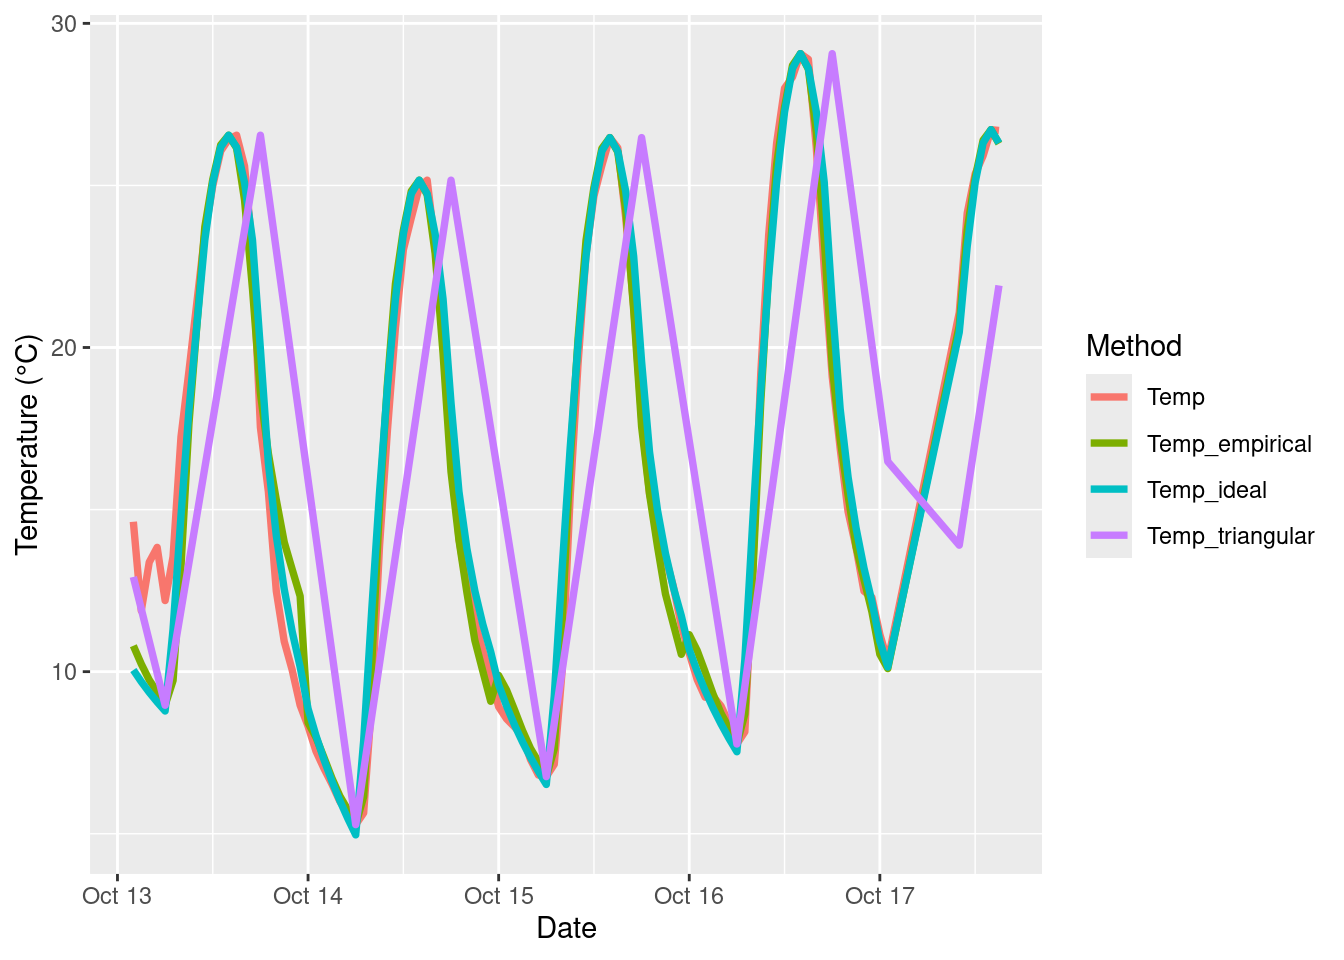
\includegraphics{Book_files/figure-latex/empi_temps_plot_4-1.pdf}

This plots shows that the triangular curve is quite far off the mark. \texttt{Temp\_empirical} and \texttt{Temp\_ideal} look pretty similar and are hard to distinguish.

We can compare these curves a bit more thoroughly by computing, for example, the \emph{Root Mean Square Error}, which is useful for quantifying the correspondence between predicted and observed values. \texttt{chillR} has a function for this:

\begin{Shaded}
\begin{Highlighting}[]
\CommentTok{# here's the RMSE for the triangular method:}
\KeywordTok{RMSEP}\NormalTok{(Winters_temps}\OperatorTok{$}\NormalTok{Temp_triangular,Winters_temps}\OperatorTok{$}\NormalTok{Temp)}
\end{Highlighting}
\end{Shaded}

\begin{verbatim}
## [1] 4.695289
\end{verbatim}

\begin{Shaded}
\begin{Highlighting}[]
\CommentTok{# here's the RMSE for the idealized-curve method:}
\KeywordTok{RMSEP}\NormalTok{(Winters_temps}\OperatorTok{$}\NormalTok{Temp_ideal,Winters_temps}\OperatorTok{$}\NormalTok{Temp)}
\end{Highlighting}
\end{Shaded}

\begin{verbatim}
## [1] 1.576876
\end{verbatim}

\begin{Shaded}
\begin{Highlighting}[]
\CommentTok{# and here's the RMSE for the empirical-curve method:}
\KeywordTok{RMSEP}\NormalTok{(Winters_temps}\OperatorTok{$}\NormalTok{Temp_empirical,Winters_temps}\OperatorTok{$}\NormalTok{Temp)}
\end{Highlighting}
\end{Shaded}

\begin{verbatim}
## [1] 1.410625
\end{verbatim}

As you see, we get an RMSE of 4.7 for the triangular method, an RMSE of 1.58 for the idealized-curve method, and an RMSE of 1.41 for the empirical-curve method. Since this metric should be low, we see that calibrating the prediction function with observed hourly data brought some advantages, in particular when compared with the triangular method.

You may wonder if this makes much of a difference, when we want to model chill accumulation or something like that. Well, you may be able to test that already (spoiler alert: it often matters quite a bit)!

\hypertarget{exercises_hourly}{%
\section*{\texorpdfstring{\texttt{Exercises} on hourly temperatures}{Exercises on hourly temperatures}}\label{exercises_hourly}}
\addcontentsline{toc}{section}{\texttt{Exercises} on hourly temperatures}

Please document all results of the following assignments in your \texttt{learning\ logbook}.

\begin{enumerate}
\def\labelenumi{\arabic{enumi})}
\tightlist
\item
  Choose a location of interest, find out its latitude and produce plots of daily sunrise, sunset and daylength
\item
  Produce an hourly dataset, based on idealized daily curves, for the \texttt{KA\_weather} dataset (included in \texttt{chillR})
\item
  Produce empirical temperature curve parameters for the \texttt{Winters\_hours\_gaps} dataset, and use them to predict hourly values from daily temperatures (this is very similar to the example above, but please make sure you understand what's going on)
\end{enumerate}

\hypertarget{get_temp_data}{%
\chapter{Getting temperature data}\label{get_temp_data}}

\hypertarget{goals_get_temps}{%
\section*{Learning goals for this lesson}\label{goals_get_temps}}
\addcontentsline{toc}{section}{Learning goals for this lesson}

\begin{itemize}
\tightlist
\item
  Appreciate the need for daily temperature data
\item
  Know how to get a list of promising weather stations contained in an international database
\item
  Be able to download weather data using \texttt{chillR} functions
\item
  Know how to convert downloaded data into \texttt{chillR} format
\end{itemize}

\hypertarget{temperature-data-needs}{%
\section{Temperature data needs}\label{temperature-data-needs}}

Obviously, without temperature data we can't do much phenology and chill modeling. This is a pretty critical input to all models we can make or may want to run. It also seems like an easy-to-find resource, doesn't it? Well, you may be surprised by how difficult it is to get such data. While all countries in the world have official weather stations that record precisely the type of information we need, many are very protective of these data. Many national weather services sell such information (the collection of which was likely funded by taxpayer money) at rather high prices. If you only want to do a study on one location, you may be able to shell out that money, but this quickly becomes unrealistic, when you're targeting a larger-scale analysis.

On a personal note, I must say that I find it pretty outrageous that at a time where we should be making every effort to understand the impacts of climate change on our world and to find ways to adapt, weather services are putting up such access barriers. I really wonder how many climate-related studies that have been done turned out less useful than they could have been, had more data been easily and freely available. Well, back to the main story\ldots{}

To be clear, it's of course preferable to have a high-quality dataset collected in the exact place that you want to analyze. If we don't have such data, however, there are a few databases out there that we can draw on as an alternative option. \texttt{chillR} currently has the capability to access one global database, as well as one for California. There is certainly scope for expanding this capability, but let's start working with what's available now.

\hypertarget{the-global-summary-of-the-day-database}{%
\section{The Global Summary of the Day database}\label{the-global-summary-of-the-day-database}}

An invaluable source of temperature data is the \href{https://www.ncei.noaa.gov/}{National Centers for Environmental Information (NCEI)}, formerly the National Climatic Data Center (NCDC) of the \href{https://www.noaa.gov/}{United States National Oceanic and Atmospheric Administration (NOAA)}, in particular their \href{https://www.ncei.noaa.gov/access/search/data-search/global-summary-of-the-day}{Global Summary of the Day (GSOD) database}. That was a pretty long name, so let's stick with the abbreviation \texttt{GSOD}.

Check out the \href{https://www.ncei.noaa.gov/access/search/data-search/global-summary-of-the-day}{GSOD website} to take a look at the interface: \url{https://www.ncei.noaa.gov/access/search/data-search/global-summary-of-the-day}. This interface used to be pretty confusing in the past - and I almost find it more confusing now. Fortunately, if you click on the \texttt{Bulk\ downloads} button, you can get to a place where you can directly access the weather data: \url{https://www.ncei.noaa.gov/data/global-summary-of-the-day/access/}. What we find here is, at first glance, even more inaccessible than the web interface, but at least we can recognize some structure now: All records are stored in separate files for each station and year, with the files named according to a code assigned to the weather stations. You could now download these records by hand, if you wanted to, but this would take a long time (if you want data for many years), and you'd first have to find out what station is of interest to you.

Fortunately, I found a list of all the weather stations somewhere on NOAA's website: \url{ftp://ftp.ncdc.noaa.gov/pub/data/noaa/isd-history.csv}, and I automated the tedious data download and assembling process in \texttt{chillR}. Let's see how this works:

There's a single \texttt{chillR} function, \texttt{handle\_gsod()}, that can take care of all data retrieval steps. Since there are multiple steps involved, we have to use the function's \texttt{action} parameter to tell it what to do:

\hypertarget{actionlist_stations}{%
\subsection{\texorpdfstring{\texttt{action=list\_stations}}{action=list\_stations}}\label{actionlist_stations}}

When used with this action, \texttt{handle\_gsod()} retrieves the station list and sorts them based on their proximity to a set of coordinates we specify. Let's look for stations around Bonn (Latitude= 50.73; Longitude= 7.10). I'll also add a time interval of interest (1990-2020) to narrow the search.

\begin{Shaded}
\begin{Highlighting}[]
\NormalTok{station_list<-}\KeywordTok{handle_gsod}\NormalTok{(}\DataTypeTok{action=}\StringTok{"list_stations"}\NormalTok{,}
                          \DataTypeTok{location=}\KeywordTok{c}\NormalTok{(}\FloatTok{7.10}\NormalTok{,}\FloatTok{50.73}\NormalTok{),}
                          \DataTypeTok{time_interval=}\KeywordTok{c}\NormalTok{(}\DecValTok{1990}\NormalTok{,}\DecValTok{2020}\NormalTok{))}
\end{Highlighting}
\end{Shaded}

\begin{Shaded}
\begin{Highlighting}[]
\KeywordTok{require}\NormalTok{(kableExtra)}

\KeywordTok{kable}\NormalTok{(station_list) }\OperatorTok
\StringTok{  }\KeywordTok{kable_styling}\NormalTok{(}\StringTok{"striped"}\NormalTok{, }\DataTypeTok{position =} \StringTok{"left"}\NormalTok{, }\DataTypeTok{font_size =} \DecValTok{8}\NormalTok{)}
\end{Highlighting}
\end{Shaded}

\begingroup\fontsize{8}{10}\selectfont

\begin{tabular}{l|l|l|r|r|r|r|r|r|r}
\hline
chillR\_code & STATION.NAME & CTRY & Lat & Long & BEGIN & END & distance & Overlap\_years & Perc\_interval\_covered\\
\hline
105170\_99999 & BONN/FRIESDORF(AUT) & GM & 50.70 & 7.15 & 19360102 & 19921231 & 4.86 & 3.00 & 9.77\\
\hline
105180\_99999 & BONN-HARDTHOEHE & GM & 50.70 & 7033.00 & 19750523 & 20031030 & 5.79 & 13.83 & 45.02\\
\hline
105190\_99999 & BONN-ROLEBER & GM & 50733.00 & 7.20 & 20010705 & 20081231 & 7.07 & 7.49 & 24.39\\
\hline
105130\_99999 & KOLN BONN & GM & 50866.00 & 7143.00 & 19310101 & 20200917 & 15.43 & 30.71 & 99.98\\
\hline
105090\_99999 & BUTZWEILERHOF(BAFB) & GM & 50983.00 & 6.90 & 19780901 & 19950823 & 31.47 & 5.64 & 18.37\\
\hline
105020\_99999 & NORVENICH & GM & 50831.00 & 6658.00 & 19730101 & 20200917 & 33.14 & 30.71 & 99.98\\
\hline
105140\_99999 & MENDIG & GM & 50366.00 & 7315.00 & 19730102 & 20070614 & 43.26 & 17.45 & 56.81\\
\hline
105060\_99999 & NUERBURG-BARWEILER & GM & 50367.00 & 6867.00 & 19950401 & 20081231 & 43.63 & 13.75 & 44.77\\
\hline
105080\_99999 & BLANKENHEIM & GM & 50.45 & 6.65 & 19781002 & 19840504 & 44.56 & 0.00 & 0.00\\
\hline
105100\_99999 & NUERBURG & GM & 50333.00 & 6.95 & 19300901 & 19921231 & 45.42 & 3.00 & 9.77\\
\hline
105150\_99999 & BENDORF & GM & 50417.00 & 7583.00 & 19310102 & 20030816 & 48.82 & 13.62 & 44.35\\
\hline
105040\_99999 & EIFEL & GM & 50.65 & 6283.00 & 20040501 & 20040501 & 58.41 & 0.00 & 0.01\\
\hline
105260\_99999 & BAD MARIENBERG & GM & 50667.00 & 7967.00 & 19730101 & 20030816 & 61.65 & 13.62 & 44.35\\
\hline
106130\_99999 & BUCHEL & GM & 50174.00 & 7063.00 & 19730101 & 20200917 & 61.90 & 30.71 & 99.98\\
\hline
105030\_99999 & AACHEN/MERZBRUCK & GM & 50817.00 & 6183.00 & 19780901 & 20030305 & 65.40 & 13.18 & 42.89\\
\hline
104190\_99999 & LUDENSCHEID       \& & GM & 51233.00 & 7.60 & 19270906 & 20030306 & 66.06 & 13.18 & 42.90\\
\hline
104000\_99999 & DUSSELDORF & GM & 51289.00 & 6767.00 & 19310102 & 20200917 & 66.43 & 30.71 & 99.98\\
\hline
106162\_99999 & SIEGERLAND & GM & 50708.00 & 8083.00 & 20040510 & 20200917 & 69.46 & 16.36 & 53.25\\
\hline
104180\_99999 & LUEDENSCHEID & GM & 51.25 & 7.65 & 19940301 & 20081231 & 69.55 & 14.84 & 48.30\\
\hline
104374\_99999 & MONCHENGLADBACH & GM & 51.23 & 6504.00 & 19960715 & 20200917 & 69.61 & 24.18 & 78.70\\
\hline
104030\_99999 & MOENCHENGLADBACH & GM & 51233.00 & 6.50 & 19381001 & 19421031 & 70.05 & 0.00 & 0.00\\
\hline
105010\_99999 & AACHEN & GM & 50783.00 & 6.10 & 19280101 & 20030816 & 70.81 & 13.62 & 44.35\\
\hline
064960\_99999 & ELSENBORN (MIL) & BE & 50467.00 & 6183.00 & 19840501 & 20200917 & 71.21 & 30.71 & 99.98\\
\hline
104090\_99999 & ESSEN/MUELHEIM & GM & 51.40 & 6967.00 & 19300414 & 19431231 & 75.12 & 0.00 & 0.00\\
\hline
104100\_99999 & ESSEN/MULHEIM & GM & 51.40 & 6967.00 & 19310101 & 20030816 & 75.12 & 13.62 & 44.35\\
\hline
\end{tabular}
\endgroup{}

This list contains the 25 closest stations to the location we entered, ordered by their distance to the target coordinates. This distance is shown in the \texttt{distance} column. The \texttt{Overlap\_years} column shows the number of years that are available, and the \texttt{Perc\_interval\_covered} column the percentage of the target interval that is covered. Note that this is only based on the \texttt{BEGIN} and \texttt{END} dates in the table - it's quite possible (and usually the case) that the dataset contains gaps, which sometimes cover almost the entire record.

\hypertarget{actiondownload_weather}{%
\subsection{\texorpdfstring{\texttt{action="download\_weather"}}{action="download\_weather"}}\label{actiondownload_weather}}

When used with this option, the \texttt{handle\_gsod()} function downloads the weather data for a particular station, based on a station-specific \texttt{chillR\_code} (shown in the respective column of the table above). Rather than typing the code manually, we can refer to the code in the station\_list. Let's download the data for the 4\textsuperscript{th} entry in the list, which looks like it covers most of the period we're interested in.

\begin{Shaded}
\begin{Highlighting}[]
\NormalTok{weather<-}\KeywordTok{handle_gsod}\NormalTok{(}\DataTypeTok{action=}\StringTok{"download_weather"}\NormalTok{,}
                     \DataTypeTok{location=}\NormalTok{station_list}\OperatorTok{$}\NormalTok{chillR_code[}\DecValTok{4}\NormalTok{],}
                     \DataTypeTok{time_interval=}\KeywordTok{c}\NormalTok{(}\DecValTok{1990}\NormalTok{,}\DecValTok{2020}\NormalTok{))}
\end{Highlighting}
\end{Shaded}

The result of this operation is a list with two elements. Element 1 (\texttt{weather{[}{[}1{]}{]}}) is an indication of the database the data come from. Element 2 (\texttt{weather{[}{[}2{]}{]}}) is the actual dataset, which we can see here:

\begin{Shaded}
\begin{Highlighting}[]
\KeywordTok{kable}\NormalTok{(weather}\OperatorTok{$}\NormalTok{weather[}\DecValTok{1}\OperatorTok{:}\DecValTok{20}\NormalTok{,]) }\OperatorTok
\StringTok{  }\KeywordTok{kable_styling}\NormalTok{(}\StringTok{"striped"}\NormalTok{, }\DataTypeTok{position =} \StringTok{"left"}\NormalTok{, }\DataTypeTok{font_size =} \DecValTok{8}\NormalTok{)}
\end{Highlighting}
\end{Shaded}

\begingroup\fontsize{8}{10}\selectfont

\begin{tabular}{l|r|r|r|r|r|r|r|r|r|r|r|r|r|r|r|r|r|r|r|r|l|r|l|r|l|r|r|r|r|r}
\hline
DATE & STN... & WBAN & YEAR & MONTH & DAY & TEMP & Count1 & DEWP & Count2 & SLP & Count3 & STP & Count4 & VISIB & Count5 & WDSP & Count6 & MXSPD & GUST & MAX & MaxFlag & MIN & MinFlag & PRCP & PrcpFlag & SNDP & FRSHTT & Year & Month & Day\\
\hline
1990-01-01 12:00:00 & 105130 & 99999 & 1990 & 1 & 1 & 0.0000000 & 24 & 30.1 & 24 & NA & 0 & NA & 0 & 5.3 & 24 & 5.8 & 24 & 8.9 & NA & 1.000000 & * & -1.0000000 & * & 0 & F & NA & 10000 & 1990 & 1 & 1\\
\hline
1990-01-02 12:00:00 & 105130 & 99999 & 1990 & 1 & 2 & 1.0000000 & 24 & 31.8 & 24 & NA & 0 & NA & 0 & 3.6 & 24 & 4.5 & 24 & 9.9 & NA & 2.000000 & * & 0.0000000 & * & 0 & G & NA & 110000 & 1990 & 1 & 2\\
\hline
1990-01-03 12:00:00 & 105130 & 99999 & 1990 & 1 & 3 & 0.7222222 & 24 & 29.9 & 24 & NA & 0 & NA & 0 & 5.9 & 24 & 10.3 & 24 & 15.9 & NA & 2.000000 & * & -0.3888889 & * & 0 & G & NA & 100000 & 1990 & 1 & 3\\
\hline
1990-01-04 12:00:00 & 105130 & 99999 & 1990 & 1 & 4 & -0.0555556 & 24 & 27.2 & 24 & NA & 0 & NA & 0 & 5.2 & 24 & 10.1 & 24 & 17.1 & NA & 2.000000 & * & -1.1111111 & * & 0 & D & NA & 10000 & 1990 & 1 & 4\\
\hline
1990-01-05 12:00:00 & 105130 & 99999 & 1990 & 1 & 5 & 1.5555556 & 24 & 31.8 & 24 & NA & 0 & NA & 0 & 4.4 & 24 & 3.8 & 24 & 6.0 & NA & 3.111111 &  & -1.1111111 &  & 0 & G & NA & 10000 & 1990 & 1 & 5\\
\hline
1990-01-06 12:00:00 & 105130 & 99999 & 1990 & 1 & 6 & 1.3333333 & 24 & 31.1 & 24 & NA & 0 & NA & 0 & 6.6 & 24 & 11.5 & 24 & 15.0 & NA & 2.388889 &  & 0.0000000 & * & 0 & G & NA & 0 & 1990 & 1 & 6\\
\hline
1990-01-07 12:00:00 & 105130 & 99999 & 1990 & 1 & 7 & 1.0555556 & 24 & 29.7 & 24 & NA & 0 & NA & 0 & 6.2 & 24 & 10.7 & 24 & 15.9 & NA & 4.277778 &  & -0.1111111 & * & 0 & D & NA & 0 & 1990 & 1 & 7\\
\hline
1990-01-08 12:00:00 & 105130 & 99999 & 1990 & 1 & 8 & 3.2777778 & 24 & 34.0 & 24 & NA & 0 & NA & 0 & 6.0 & 24 & 7.1 & 24 & 9.9 & NA & 7.000000 & * & -0.1111111 &  & 0 & G & NA & 10000 & 1990 & 1 & 8\\
\hline
1990-01-09 12:00:00 & 105130 & 99999 & 1990 & 1 & 9 & 5.3333333 & 24 & 38.5 & 24 & NA & 0 & NA & 0 & 5.4 & 24 & 5.3 & 24 & 11.1 & NA & 8.000000 &  & 3.7777778 &  & 508 & G & NA & 10000 & 1990 & 1 & 9\\
\hline
1990-01-10 12:00:00 & 105130 & 99999 & 1990 & 1 & 10 & 4.5555556 & 24 & 37.4 & 24 & NA & 0 & NA & 0 & 4.8 & 24 & 5.9 & 24 & 8.0 & NA & 6.000000 &  & 3.0000000 & * & 1016 & G & NA & 10010 & 1990 & 1 & 10\\
\hline
1990-01-11 12:00:00 & 105130 & 99999 & 1990 & 1 & 11 & 5.1666667 & 24 & 35.9 & 24 & NA & 0 & NA & 0 & 8.1 & 24 & 6.4 & 24 & 8.9 & NA & 7.000000 & * & 3.2777778 &  & 254 & G & NA & 10000 & 1990 & 1 & 11\\
\hline
1990-01-12 12:00:00 & 105130 & 99999 & 1990 & 1 & 12 & 1.7777778 & 24 & 31.2 & 24 & NA & 0 & NA & 0 & 7.2 & 24 & 8.7 & 24 & 13.0 & NA & 5.222222 & * & -1.0000000 & * & 0 & G & NA & 0 & 1990 & 1 & 12\\
\hline
1990-01-13 12:00:00 & 105130 & 99999 & 1990 & 1 & 13 & 1.3888889 & 24 & 31.7 & 24 & 1028.1 & 4 & 1015.5 & 4 & 6.2 & 24 & 6.8 & 24 & 11.1 & NA & 4.000000 & * & -1.2777778 &  & 0 & D & NA & 0 & 1990 & 1 & 13\\
\hline
1990-01-14 12:00:00 & 105130 & 99999 & 1990 & 1 & 14 & 3.1666667 & 24 & 35.5 & 24 & NA & 0 & NA & 0 & 5.3 & 24 & 4.7 & 24 & 8.0 & NA & 5.000000 & * & -0.2222222 &  & 0 & C & NA & 10000 & 1990 & 1 & 14\\
\hline
1990-01-15 12:00:00 & 105130 & 99999 & 1990 & 1 & 15 & 4.5555556 & 24 & 37.5 & 24 & NA & 0 & NA & 0 & 6.6 & 24 & 7.4 & 24 & 11.1 & NA & 9.000000 & * & 0.8888889 &  & 1016 & F & NA & 10000 & 1990 & 1 & 15\\
\hline
1990-01-16 12:00:00 & 105130 & 99999 & 1990 & 1 & 16 & 9.9444444 & 24 & 45.0 & 24 & NA & 0 & NA & 0 & 7.8 & 24 & 7.1 & 24 & 14.0 & 27 & 11.000000 &  & 6.2222222 &  & 0 & F & NA & 10000 & 1990 & 1 & 16\\
\hline
1990-01-17 12:00:00 & 105130 & 99999 & 1990 & 1 & 17 & 8.5000000 & 24 & 40.2 & 24 & NA & 0 & NA & 0 & 7.3 & 24 & 10.1 & 24 & 17.1 & 35 & 11.000000 & * & 1.0000000 & * & 0 & G & NA & 10000 & 1990 & 1 & 17\\
\hline
1990-01-18 12:00:00 & 105130 & 99999 & 1990 & 1 & 18 & 2.7222222 & 24 & 32.2 & 24 & NA & 0 & NA & 0 & 7.6 & 24 & 5.8 & 24 & 12.0 & NA & 7.000000 & * & -1.0000000 & * & 254 & G & NA & 0 & 1990 & 1 & 18\\
\hline
1990-01-19 12:00:00 & 105130 & 99999 & 1990 & 1 & 19 & 4.6111111 & 24 & 33.3 & 24 & NA & 0 & NA & 0 & 7.2 & 24 & 7.5 & 24 & 14.0 & NA & 7.111111 &  & 2.0000000 &  & 0 & G & NA & 10000 & 1990 & 1 & 19\\
\hline
1990-01-20 12:00:00 & 105130 & 99999 & 1990 & 1 & 20 & 6.0555556 & 24 & 38.7 & 24 & 1024.9 & 4 & 1012.5 & 4 & 9.1 & 24 & 8.5 & 24 & 14.0 & NA & 8.500000 &  & 4.0000000 &  & 2286 & G & NA & 10000 & 1990 & 1 & 20\\
\hline
\end{tabular}
\endgroup{}

This still looks pretty complicated, and it contains a lot of information we don't need. \texttt{chillR} therefore contains a function to simplify this record. Note, however, that this removes a lot of variables you may be interested in. More importantly, this also removes quality flags, which may indicate that particular records aren't reliable. I've generously ignored this so far, but there's room for improvement here.

\hypertarget{downloaded-weather-as-action-argument}{%
\subsection{\texorpdfstring{downloaded weather as \texttt{action} argument}{downloaded weather as action argument}}\label{downloaded-weather-as-action-argument}}

This way of calling \texttt{handle\_gsod()} serves to clean the dataset and convert it into a format that \texttt{chillR} can easily handle

\begin{Shaded}
\begin{Highlighting}[]
\NormalTok{cleaned_weather<-}\KeywordTok{handle_gsod}\NormalTok{(weather)}
\end{Highlighting}
\end{Shaded}

\begin{Shaded}
\begin{Highlighting}[]
\KeywordTok{kable}\NormalTok{(cleaned_weather}\OperatorTok{$}\NormalTok{weather[}\DecValTok{1}\OperatorTok{:}\DecValTok{20}\NormalTok{,]) }\OperatorTok
\StringTok{  }\KeywordTok{kable_styling}\NormalTok{(}\StringTok{"striped"}\NormalTok{, }\DataTypeTok{position =} \StringTok{"left"}\NormalTok{, }\DataTypeTok{font_size =} \DecValTok{8}\NormalTok{)}
\end{Highlighting}
\end{Shaded}

\begingroup\fontsize{8}{10}\selectfont

\begin{tabular}{r|r|r|r|r|r|r}
\hline
Year & Month & Day & Tmin & Tmax & Tmean & Prec\\
\hline
1990 & 1 & 1 & -1.0000000 & 1.000000 & 0.0000000 & 0.000\\
\hline
1990 & 1 & 2 & 0.0000000 & 2.000000 & 1.0000000 & 0.000\\
\hline
1990 & 1 & 3 & -0.3888889 & 2.000000 & 0.7222222 & 0.000\\
\hline
1990 & 1 & 4 & -1.1111111 & 2.000000 & -0.0555556 & 0.000\\
\hline
1990 & 1 & 5 & -1.1111111 & 3.111111 & 1.5555556 & 0.000\\
\hline
1990 & 1 & 6 & 0.0000000 & 2.388889 & 1.3333333 & 0.000\\
\hline
1990 & 1 & 7 & -0.1111111 & 4.277778 & 1.0555556 & 0.000\\
\hline
1990 & 1 & 8 & -0.1111111 & 7.000000 & 3.2777778 & 0.000\\
\hline
1990 & 1 & 9 & 3.7777778 & 8.000000 & 5.3333333 & 0.508\\
\hline
1990 & 1 & 10 & 3.0000000 & 6.000000 & 4.5555556 & 1.016\\
\hline
1990 & 1 & 11 & 3.2777778 & 7.000000 & 5.1666667 & 0.254\\
\hline
1990 & 1 & 12 & -1.0000000 & 5.222222 & 1.7777778 & 0.000\\
\hline
1990 & 1 & 13 & -1.2777778 & 4.000000 & 1.3888889 & 0.000\\
\hline
1990 & 1 & 14 & -0.2222222 & 5.000000 & 3.1666667 & 0.000\\
\hline
1990 & 1 & 15 & 0.8888889 & 9.000000 & 4.5555556 & 1.016\\
\hline
1990 & 1 & 16 & 6.2222222 & 11.000000 & 9.9444444 & 0.000\\
\hline
1990 & 1 & 17 & 1.0000000 & 11.000000 & 8.5000000 & 0.000\\
\hline
1990 & 1 & 18 & -1.0000000 & 7.000000 & 2.7222222 & 0.254\\
\hline
1990 & 1 & 19 & 2.0000000 & 7.111111 & 4.6111111 & 0.000\\
\hline
1990 & 1 & 20 & 4.0000000 & 8.500000 & 6.0555556 & 2.286\\
\hline
\end{tabular}
\endgroup{}

Note that the reason for many of the strange numbers in these records is that the original database stores them in degrees Fahrenheit, so that they had to be converted to degrees Celsius. That often creates ugly numbers, but it's not hard:

\(Temperature[°C]=(Temperature[°F]-32)\cdot\frac{5}{9}\)

We now have a temperature record in a format that we can easily work with in \texttt{chillR}.

Upon closer inspection, however, you'll notice that this dataset has pretty substantial gaps, including several entire years of missing data. How can we deal with this? Let's find out in the lesson on \protect\hyperlink{filling-gaps-in-temperature-records}{Filling gaps in temperature records}.

Note that \texttt{chillR} has a pretty similar function to download data from the \href{https://cimis.water.ca.gov/}{California Irrigation Management Information System (CIMIS)}.

There's surely room for improvement here. There's a lot more data out there that \texttt{chillR} could have a download function for.

Now let's save the files we generated here, so that we can use them in the upcoming chapters:

\begin{Shaded}
\begin{Highlighting}[]
\KeywordTok{write.csv}\NormalTok{(station_list,}\StringTok{"data/station_list.csv"}\NormalTok{,}\DataTypeTok{row.names=}\OtherTok{FALSE}\NormalTok{)}
\KeywordTok{write.csv}\NormalTok{(weather,}\StringTok{"data/Bonn_weather.csv"}\NormalTok{,}\DataTypeTok{row.names=}\OtherTok{FALSE}\NormalTok{)}
\KeywordTok{write.csv}\NormalTok{(cleaned_weather}\OperatorTok{$}\NormalTok{weather,}\StringTok{"data/Bonn_chillR_weather.csv"}\NormalTok{,}\DataTypeTok{row.names=}\OtherTok{FALSE}\NormalTok{)}
\KeywordTok{write.csv}\NormalTok{(cleaned_weather}\OperatorTok{$}\NormalTok{QC,}\StringTok{"data/Bonn_chillR_QC.csv"}\NormalTok{,}\DataTypeTok{row.names=}\OtherTok{FALSE}\NormalTok{)}
\end{Highlighting}
\end{Shaded}

\hypertarget{exercises_getting}{%
\section*{\texorpdfstring{\texttt{Exercises} on getting temperature data}{Exercises on getting temperature data}}\label{exercises_getting}}
\addcontentsline{toc}{section}{\texttt{Exercises} on getting temperature data}

Please document all results of the following assignments in your \texttt{learning\ logbook}.

\begin{enumerate}
\def\labelenumi{\arabic{enumi})}
\tightlist
\item
  Choose a location of interest and find the 25 closest weather stations using the \texttt{handle\_gsod} function
\item
  Download weather data for the most promising station on the list
\item
  Convert the weather data into \texttt{chillR} format
\end{enumerate}

\hypertarget{filling-gaps-in-temperature-records}{%
\chapter{Filling gaps in temperature records}\label{filling-gaps-in-temperature-records}}

\hypertarget{goals_gaps}{%
\section*{Learning goals for this lesson}\label{goals_gaps}}
\addcontentsline{toc}{section}{Learning goals for this lesson}

\begin{itemize}
\tightlist
\item
  see why having gaps in records can be quite problematic
\item
  learn about (too?) simple ways to fill gaps in daily temperature records
\item
  learn how to use data from auxiliary weather stations to fill gaps in daily temperature records
\item
  learn about a creative way to close gaps in hourly temperature records
\end{itemize}

\hypertarget{gaps}{%
\section{Gaps}\label{gaps}}

There's a lot of weather data out there, but most of it isn't perfect. Lots of things can go wrong when recording temperature data, including malfunctioning equipment, flat batteries, power cuts or lack of maintenance. Data archiving, transmission and storage in a database presents the next hurdle. Many datasets therefore have gaps that can be very annoying when you're trying to model agroclimatic conditions. Many scientific methods don't deal very well with missing data. So we need ways of filling such gaps.

\hypertarget{filling-short-gaps-in-daily-records}{%
\section{Filling short gaps in daily records}\label{filling-short-gaps-in-daily-records}}

Weather records may be largely complete, except for isolated incidences of missing daily minimum or maximum temperatures. In such cases, we may get away with simple linear interpolation. This means, we take the last recorded value before a gaps and the first after the gap and compute the average. We can use equivalent procedures for slightly longer gaps (e.g.~2-3 day), and possibly even a few more (even though we should now be starting to feel a bit uneasy about this). Obviously, the longer the gaps, the more dubious this practice becomes. In case gaps extend to several weeks or even months, linear interpolation, which simply connects the start and end points of the gap by a straight line, may miss important features of the local temperature dynamics. In the extreme case, where we're missing an entire year of data, such linear interpolation would miss entire seasons, producing unacceptable errors. Yet \texttt{chillR} has a function to implement such simple interpolation - \texttt{interpolate\_gaps()}.

\begin{Shaded}
\begin{Highlighting}[]
\KeywordTok{library}\NormalTok{(chillR)}
\NormalTok{weather<-}\KeywordTok{make_all_day_table}\NormalTok{(KA_weather)}
\NormalTok{Tmin_int<-}\KeywordTok{interpolate_gaps}\NormalTok{(KA_weather[,}\StringTok{"Tmin"}\NormalTok{])}
\NormalTok{weather[,}\StringTok{"Tmin"}\NormalTok{]<-Tmin_int}\OperatorTok{$}\NormalTok{interp}
\NormalTok{weather[,}\StringTok{"Tmin_interpolated"}\NormalTok{]<-Tmin_int}\OperatorTok{$}\NormalTok{missing}

\NormalTok{Tmax_int<-}\KeywordTok{interpolate_gaps}\NormalTok{(KA_weather[,}\StringTok{"Tmax"}\NormalTok{])}
\NormalTok{weather[,}\StringTok{"Tmax"}\NormalTok{]<-Tmax_int}\OperatorTok{$}\NormalTok{interp}
\NormalTok{weather[,}\StringTok{"Tmax_interpolated"}\NormalTok{]<-Tmax_int}\OperatorTok{$}\NormalTok{missing}
\end{Highlighting}
\end{Shaded}

The \texttt{fix\_weather()} function in \texttt{chillR} uses the same procedure. If you run this without any arguments (just \texttt{fix\_weather(weather)}), this function assumes you're trying to linearly interpolate all gaps in the \texttt{Tmin} and \texttt{Tmax} columns. If entire days are missing in the records, new lines are added for these days (using the \texttt{make\_all\_day\_table()} function). You can also specify the range of years to apply this procedure for (by specifying \texttt{start\_year} and \texttt{end\_year}), the dates to work on (\texttt{start\_date} and \texttt{end\_date} - these are in Julian days, i.e.~days of the year) and the names of columns you want to work on (needed if these are different from \texttt{Tmin} and \texttt{Tmax})

\begin{Shaded}
\begin{Highlighting}[]
\CommentTok{# add an extra day to the KA_weather dataset that is not connected to the days that are already there.}
\CommentTok{# this creates a large gap, which we can then interpolate}
\NormalTok{KA_weather_gap<-}\KeywordTok{rbind}\NormalTok{(KA_weather,}\KeywordTok{c}\NormalTok{(}\DataTypeTok{Year=}\DecValTok{2011}\NormalTok{,}\DataTypeTok{Month=}\DecValTok{3}\NormalTok{,}\DataTypeTok{Day=}\DecValTok{3}\NormalTok{,}\DataTypeTok{Tmax=}\DecValTok{26}\NormalTok{,}\DataTypeTok{Tmin=}\DecValTok{14}\NormalTok{)) }

\CommentTok{# fill in the gaps between Julian date 300 (late October) and 100 (early April), only returning data between 2000 and 2011}
\NormalTok{fixed_winter_days<-}\KeywordTok{fix_weather}\NormalTok{(KA_weather_gap, }\DataTypeTok{start_year=}\DecValTok{2000}\NormalTok{, }\DataTypeTok{end_year=}\DecValTok{2011}\NormalTok{, }\DataTypeTok{start_date=}\DecValTok{300}\NormalTok{, }\DataTypeTok{end_date=}\DecValTok{100}\NormalTok{)}

\CommentTok{# fill in all gaps}
\NormalTok{fixed_all_days<-}\KeywordTok{fix_weather}\NormalTok{(KA_weather_gap)}
\end{Highlighting}
\end{Shaded}

The \texttt{fix\_weather()} function produces a list with two outputs:

\begin{itemize}
\item
  \texttt{weather}: a \texttt{data.frame} with the interpolated weather data, now including columns \texttt{no\_Tmin} and \texttt{no\_Tmax}, which appear as \texttt{TRUE}, when the respective values were originally missing (\texttt{FALSE} otherwise)
\item
  \texttt{QC}: a quality control object that summarizes how many values were interpolated for each season.
\end{itemize}

Here's how the QC elements look for the two interpolated datasets we just created:

\begin{Shaded}
\begin{Highlighting}[]
\KeywordTok{kable}\NormalTok{(fixed_winter_days}\OperatorTok{$}\NormalTok{QC, }\DataTypeTok{caption=}\StringTok{"Quality control summary produced by *fix_weather()*, with only winter days interpolated"}\NormalTok{) }\OperatorTok
\StringTok{  }\KeywordTok{kable_styling}\NormalTok{(}\StringTok{"striped"}\NormalTok{, }\DataTypeTok{position =} \StringTok{"left"}\NormalTok{, }\DataTypeTok{font_size =} \DecValTok{10}\NormalTok{)}
\end{Highlighting}
\end{Shaded}

\textbackslash begin\{table\}

\textbackslash caption\{\label{tab:unnamed-chunk-7}Quality control summary produced by \emph{fix\_weather()}, with only winter days interpolated\}
\fontsize{10}{12}\selectfont

\begin{tabular}[t]{l|r|r|r|r|r|r|r}
\hline
Season & End\_year & Season\_days & Data\_days & Missing\_Tmin & Missing\_Tmax & Incomplete\_days & Perc\_complete\\
\hline
1999/2000 & 2000 & 166 & 100 & 66 & 66 & 66 & 60.2\\
\hline
2000/2001 & 2001 & 167 & 167 & 0 & 0 & 0 & 100.0\\
\hline
2001/2002 & 2002 & 166 & 166 & 0 & 0 & 0 & 100.0\\
\hline
2002/2003 & 2003 & 166 & 166 & 0 & 0 & 0 & 100.0\\
\hline
2003/2004 & 2004 & 166 & 166 & 0 & 0 & 0 & 100.0\\
\hline
2004/2005 & 2005 & 167 & 167 & 0 & 0 & 0 & 100.0\\
\hline
2005/2006 & 2006 & 166 & 166 & 0 & 0 & 0 & 100.0\\
\hline
2006/2007 & 2007 & 166 & 166 & 0 & 0 & 0 & 100.0\\
\hline
2007/2008 & 2008 & 166 & 166 & 0 & 0 & 0 & 100.0\\
\hline
2008/2009 & 2009 & 167 & 167 & 0 & 0 & 0 & 100.0\\
\hline
2009/2010 & 2010 & 166 & 166 & 0 & 0 & 0 & 100.0\\
\hline
2010/2011 & 2011 & 166 & 128 & 165 & 165 & 165 & 0.6\\
\hline
\end{tabular}

\textbackslash end\{table\}

\begin{Shaded}
\begin{Highlighting}[]
\KeywordTok{kable}\NormalTok{(fixed_all_days}\OperatorTok{$}\NormalTok{QC, }\DataTypeTok{caption=}\StringTok{"Quality control summary produced by *fix_weather()*, with all days interpolated"}\NormalTok{) }\OperatorTok
\StringTok{  }\KeywordTok{kable_styling}\NormalTok{(}\StringTok{"striped"}\NormalTok{, }\DataTypeTok{position =} \StringTok{"left"}\NormalTok{, }\DataTypeTok{font_size =} \DecValTok{10}\NormalTok{)}
\end{Highlighting}
\end{Shaded}

\textbackslash begin\{table\}

\textbackslash caption\{\label{tab:unnamed-chunk-8}Quality control summary produced by \emph{fix\_weather()}, with all days interpolated\}
\fontsize{10}{12}\selectfont

\begin{tabular}[t]{l|r|r|r|r|r|r|r}
\hline
Season & End\_year & Season\_days & Data\_days & Missing\_Tmin & Missing\_Tmax & Incomplete\_days & Perc\_complete\\
\hline
1997/1998 & 1998 & 365 & 365 & 0 & 0 & 0 & 100.0\\
\hline
1998/1999 & 1999 & 365 & 365 & 0 & 0 & 0 & 100.0\\
\hline
1999/2000 & 2000 & 366 & 366 & 0 & 0 & 0 & 100.0\\
\hline
2000/2001 & 2001 & 365 & 365 & 0 & 0 & 0 & 100.0\\
\hline
2001/2002 & 2002 & 365 & 365 & 0 & 0 & 0 & 100.0\\
\hline
2002/2003 & 2003 & 365 & 365 & 0 & 0 & 0 & 100.0\\
\hline
2003/2004 & 2004 & 366 & 366 & 0 & 0 & 0 & 100.0\\
\hline
2004/2005 & 2005 & 365 & 365 & 0 & 0 & 0 & 100.0\\
\hline
2005/2006 & 2006 & 365 & 365 & 0 & 0 & 0 & 100.0\\
\hline
2006/2007 & 2007 & 365 & 365 & 0 & 0 & 0 & 100.0\\
\hline
2007/2008 & 2008 & 366 & 366 & 0 & 0 & 0 & 100.0\\
\hline
2008/2009 & 2009 & 365 & 365 & 0 & 0 & 0 & 100.0\\
\hline
2009/2010 & 2010 & 365 & 365 & 214 & 214 & 214 & 41.4\\
\hline
2010/2011 & 2011 & 365 & 62 & 364 & 364 & 364 & 0.3\\
\hline
\end{tabular}

\textbackslash end\{table\}

As indicated above, linear interpolation is usually acceptable for short gaps in the records, but it gets increasingly less convincing, when the gaps are longer. Here's a quick demonstration of this:

\begin{Shaded}
\begin{Highlighting}[]
\NormalTok{gap_weather<-KA_weather[}\DecValTok{200}\OperatorTok{:}\DecValTok{305}\NormalTok{,]}
\NormalTok{gap_weather[,}\StringTok{"Tmin_observed"}\NormalTok{]<-gap_weather}\OperatorTok{$}\NormalTok{Tmin}
\NormalTok{gap_weather}\OperatorTok{$}\NormalTok{Tmin[}\KeywordTok{c}\NormalTok{(}\DecValTok{2}\NormalTok{,}\DecValTok{4}\OperatorTok{:}\DecValTok{5}\NormalTok{,}\DecValTok{7}\OperatorTok{:}\DecValTok{9}\NormalTok{,}\DecValTok{11}\OperatorTok{:}\DecValTok{14}\NormalTok{,}\DecValTok{16}\OperatorTok{:}\DecValTok{20}\NormalTok{,}\DecValTok{22}\OperatorTok{:}\DecValTok{27}\NormalTok{,}\DecValTok{29}\OperatorTok{:}\DecValTok{35}\NormalTok{,}\DecValTok{37}\OperatorTok{:}\DecValTok{44}\NormalTok{,}\DecValTok{46}\OperatorTok{:}\DecValTok{54}\NormalTok{,}\DecValTok{56}\OperatorTok{:}\DecValTok{65}\NormalTok{,}\DecValTok{67}\OperatorTok{:}\DecValTok{77}\NormalTok{,}\DecValTok{79}\OperatorTok{:}\DecValTok{90}\NormalTok{,}\DecValTok{92}\OperatorTok{:}\DecValTok{104}\NormalTok{)]<-}\OtherTok{NA}
\NormalTok{fixed_gaps<-}\KeywordTok{fix_weather}\NormalTok{(gap_weather)}\OperatorTok{$}\NormalTok{weather}

\KeywordTok{ggplot}\NormalTok{(}\DataTypeTok{data=}\NormalTok{fixed_gaps,}\KeywordTok{aes}\NormalTok{(DATE,Tmin_observed))}\OperatorTok{+}\StringTok{ }\KeywordTok{geom_line}\NormalTok{(}\DataTypeTok{lwd=}\FloatTok{1.3}\NormalTok{) }\OperatorTok{+}\StringTok{ }\KeywordTok{xlab}\NormalTok{(}\StringTok{"Date"}\NormalTok{) }\OperatorTok{+}\StringTok{ }\KeywordTok{ylab}\NormalTok{(}\StringTok{"Daily minimum temperature (°C)"}\NormalTok{) }\OperatorTok{+}
\StringTok{  }\KeywordTok{geom_line}\NormalTok{(}\DataTypeTok{data=}\NormalTok{fixed_gaps,}\KeywordTok{aes}\NormalTok{(DATE,Tmin),}\DataTypeTok{col=}\StringTok{"red"}\NormalTok{,}\DataTypeTok{lwd=}\FloatTok{1.3}\NormalTok{)}
\end{Highlighting}
\end{Shaded}

\includegraphics{Book_files/figure-latex/widening_gaps-1.pdf}

The plot above shows the originally measured values in black and the interpolated values in red. To create gaps in the record for interpolation, I removed values from the original dataset, starting with gaps of length==1 on the left, and ending up with 13 missing values on the right. As you see, temperature dynamics are captured quite well on the left, but no longer very well on the right. Here's how far off we are:

\begin{Shaded}
\begin{Highlighting}[]
\NormalTok{fixed_gaps[,}\StringTok{"error"}\NormalTok{]<-}\KeywordTok{abs}\NormalTok{(fixed_gaps}\OperatorTok{$}\NormalTok{Tmin}\OperatorTok{-}\NormalTok{fixed_gaps}\OperatorTok{$}\NormalTok{Tmin_observed)}

\KeywordTok{ggplot}\NormalTok{(}\DataTypeTok{data=}\NormalTok{fixed_gaps,}\KeywordTok{aes}\NormalTok{(DATE,error))}\OperatorTok{+}\StringTok{ }\KeywordTok{geom_line}\NormalTok{(}\DataTypeTok{lwd=}\FloatTok{1.3}\NormalTok{) }\OperatorTok{+}\StringTok{ }\KeywordTok{xlab}\NormalTok{(}\StringTok{"Date"}\NormalTok{) }\OperatorTok{+}\StringTok{ }\KeywordTok{ylab}\NormalTok{(}\StringTok{"Error introduced by interpolation (°C)"}\NormalTok{) }\OperatorTok{+}
\StringTok{  }\KeywordTok{geom_point}\NormalTok{(}\DataTypeTok{data=}\NormalTok{fixed_gaps[}\KeywordTok{which}\NormalTok{(}\OperatorTok{!}\NormalTok{fixed_gaps}\OperatorTok{$}\NormalTok{no_Tmin),],}\KeywordTok{aes}\NormalTok{(DATE,error),}\DataTypeTok{col=}\StringTok{"red"}\NormalTok{,}\DataTypeTok{cex=}\DecValTok{3}\NormalTok{)}
\end{Highlighting}
\end{Shaded}

\includegraphics{Book_files/figure-latex/gaps_error-1.pdf}

How big the errors get obviously depends on the nature of the dataset - was there a lot of variation during the period of interest, or not? Yet we see a tendency here of errors getting bigger and bigger with increasing gap sizes. Of course for the non-gap points (shown in red in the plot), the error is zero, but especially in the middle of the larger gaps, we can be quite far off from what actually happened.

For large gaps, we need a better procedure!

\hypertarget{filling-long-gaps-in-daily-records}{%
\section{Filling long gaps in daily records}\label{filling-long-gaps-in-daily-records}}

Long gaps in temperature records are a problem - and we can't make this go away entirely. To stress the obvious again: We can't know exactly what the temperatures were in a given location at a particular time, if nobody measured them. But we can make pretty good guesses. For short gaps, linear interpolation may be enough. We could now also experiment with more complex interpolation algorithms, but this is not the direction I want to take here. Instead, let's try to look for additional data that can help us deal with this challenge.

We've already learned about one good source of temperature data, and of course there are lots of other records out there. Chances are that, unless we're working way back in the past, or on a remote island, we can find another weather station that is close enough to be in a climatically comparable setting. Some researchers have identified such stations and then simply used the data from there to fill gaps for the site of interest. This (as far as I understand it) is the preferred way of dealing with gaps in records in the \href{https://cimis.water.ca.gov/}{CIMIS} network in California (at least this used to be the default option on their website).

This may work ok, if the auxiliary station is in a \emph{very} similar climatic setting, but it will already introduce an error, if we're dealing with some elevation differences, or with other landscape features that have climatic effects (e.g.~lakes, sea, forest). Such features, as well as topography, can modulate temperatures at a particular place in a way that makes them poor proxies of temperatures in another location.

\texttt{chillR} contains a function, \texttt{patch\_weather()}, that can fill gaps in a weather record based on a list of weather datasets from auxiliary stations. This function can test for (some) biases, correct data for bias ín mean temperatures, and use the result to fill gaps in the record for the location of interest.

Let's try to fill gaps in the dataset for Bonn that we downloaded in the \protect\hyperlink{get_temp_data}{Getting temperature data} lesson.

\begin{Shaded}
\begin{Highlighting}[]
\NormalTok{Bonn<-}\KeywordTok{read.csv}\NormalTok{(}\StringTok{"data/Bonn_chillR_weather.csv"}\NormalTok{)}

\NormalTok{Bonn_QC<-}\KeywordTok{fix_weather}\NormalTok{(Bonn)}\OperatorTok{$}\NormalTok{QC}

\KeywordTok{kable}\NormalTok{(Bonn_QC, }\DataTypeTok{caption=}\StringTok{"Quality control summary produced by *fix_weather()*"}\NormalTok{) }\OperatorTok
\StringTok{  }\KeywordTok{kable_styling}\NormalTok{(}\StringTok{"striped"}\NormalTok{, }\DataTypeTok{position =} \StringTok{"left"}\NormalTok{, }\DataTypeTok{font_size =} \DecValTok{10}\NormalTok{)}
\end{Highlighting}
\end{Shaded}

\textbackslash begin\{table\}

\textbackslash caption\{\label{tab:unnamed-chunk-9}Quality control summary produced by \emph{fix\_weather()}\}
\fontsize{10}{12}\selectfont

\begin{tabular}[t]{l|r|r|r|r|r|r|r}
\hline
Season & End\_year & Season\_days & Data\_days & Missing\_Tmin & Missing\_Tmax & Incomplete\_days & Perc\_complete\\
\hline
1989/1990 & 1990 & 365 & 365 & 0 & 0 & 0 & 100.0\\
\hline
1990/1991 & 1991 & 365 & 365 & 0 & 0 & 0 & 100.0\\
\hline
1991/1992 & 1992 & 366 & 366 & 0 & 0 & 0 & 100.0\\
\hline
1992/1993 & 1993 & 365 & 365 & 0 & 0 & 0 & 100.0\\
\hline
1993/1994 & 1994 & 365 & 365 & 0 & 0 & 0 & 100.0\\
\hline
1994/1995 & 1995 & 365 & 365 & 0 & 0 & 0 & 100.0\\
\hline
1995/1996 & 1996 & 366 & 366 & 0 & 0 & 0 & 100.0\\
\hline
1996/1997 & 1997 & 365 & 365 & 0 & 0 & 0 & 100.0\\
\hline
1997/1998 & 1998 & 365 & 365 & 4 & 4 & 4 & 98.9\\
\hline
1998/1999 & 1999 & 365 & 365 & 365 & 365 & 365 & 0.0\\
\hline
1999/2000 & 2000 & 366 & 366 & 366 & 366 & 366 & 0.0\\
\hline
2000/2001 & 2001 & 365 & 365 & 365 & 365 & 365 & 0.0\\
\hline
2001/2002 & 2002 & 365 & 365 & 365 & 365 & 365 & 0.0\\
\hline
2002/2003 & 2003 & 365 & 365 & 316 & 316 & 316 & 13.4\\
\hline
2003/2004 & 2004 & 366 & 366 & 366 & 366 & 366 & 0.0\\
\hline
2004/2005 & 2005 & 365 & 365 & 0 & 0 & 0 & 100.0\\
\hline
2005/2006 & 2006 & 365 & 365 & 0 & 0 & 0 & 100.0\\
\hline
2006/2007 & 2007 & 365 & 365 & 0 & 0 & 0 & 100.0\\
\hline
2007/2008 & 2008 & 366 & 366 & 366 & 366 & 366 & 0.0\\
\hline
2008/2009 & 2009 & 365 & 365 & 0 & 0 & 0 & 100.0\\
\hline
2009/2010 & 2010 & 365 & 365 & 0 & 0 & 0 & 100.0\\
\hline
2010/2011 & 2011 & 365 & 365 & 0 & 0 & 0 & 100.0\\
\hline
2011/2012 & 2012 & 366 & 366 & 0 & 0 & 0 & 100.0\\
\hline
2012/2013 & 2013 & 365 & 365 & 0 & 0 & 0 & 100.0\\
\hline
2013/2014 & 2014 & 365 & 365 & 0 & 0 & 0 & 100.0\\
\hline
2014/2015 & 2015 & 365 & 365 & 21 & 21 & 21 & 94.2\\
\hline
2015/2016 & 2016 & 366 & 366 & 0 & 0 & 0 & 100.0\\
\hline
2016/2017 & 2017 & 365 & 365 & 0 & 0 & 0 & 100.0\\
\hline
2017/2018 & 2018 & 365 & 365 & 7 & 7 & 7 & 98.1\\
\hline
2018/2019 & 2019 & 365 & 365 & 0 & 0 & 0 & 100.0\\
\hline
2019/2020 & 2020 & 366 & 366 & 105 & 105 & 105 & 71.3\\
\hline
\end{tabular}

\textbackslash end\{table\}
As you see, this dataset has substantial gaps between 1998 and 2004 and in 2008 (almost all values missing), and some shorter gaps in 2015, 2018 and 2020.

We'll now need data from other weather stations in the neighborhood. To find them, we can again use the \texttt{handle\_gsod()} function:

\begin{Shaded}
\begin{Highlighting}[]
\NormalTok{station_list<-}\KeywordTok{handle_gsod}\NormalTok{(}\DataTypeTok{action=}\StringTok{"list_stations"}\NormalTok{,}\DataTypeTok{location=}\KeywordTok{c}\NormalTok{(}\FloatTok{7.10}\NormalTok{,}\FloatTok{50.73}\NormalTok{),}\DataTypeTok{time_interval=}\KeywordTok{c}\NormalTok{(}\DecValTok{1990}\NormalTok{,}\DecValTok{2020}\NormalTok{))}
\end{Highlighting}
\end{Shaded}

\begin{Shaded}
\begin{Highlighting}[]
\KeywordTok{kable}\NormalTok{(station_list, }\DataTypeTok{caption=}\StringTok{"List of GSOD weather stations close to Bonn"}\NormalTok{) }\OperatorTok
\StringTok{  }\KeywordTok{kable_styling}\NormalTok{(}\StringTok{"striped"}\NormalTok{, }\DataTypeTok{position =} \StringTok{"left"}\NormalTok{, }\DataTypeTok{font_size =} \DecValTok{10}\NormalTok{)}
\end{Highlighting}
\end{Shaded}

\begin{table}

\caption{\label{tab:unnamed-chunk-10}List of GSOD weather stations close to Bonn}
\fontsize{10}{12}\selectfont
\begin{tabular}[t]{l|l|l|r|r|r|r|r|r|r}
\hline
chillR\_code & STATION.NAME & CTRY & Lat & Long & BEGIN & END & distance & Overlap\_years & Perc\_interval\_covered\\
\hline
105170\_99999 & BONN/FRIESDORF(AUT) & GM & 50.70 & 7.15 & 19360102 & 19921231 & 4.86 & 3.00 & 9.77\\
\hline
105180\_99999 & BONN-HARDTHOEHE & GM & 50.70 & 7033.00 & 19750523 & 20031030 & 5.79 & 13.83 & 45.02\\
\hline
105190\_99999 & BONN-ROLEBER & GM & 50733.00 & 7.20 & 20010705 & 20081231 & 7.07 & 7.49 & 24.39\\
\hline
105130\_99999 & KOLN BONN & GM & 50866.00 & 7143.00 & 19310101 & 20200917 & 15.43 & 30.71 & 99.98\\
\hline
105090\_99999 & BUTZWEILERHOF(BAFB) & GM & 50983.00 & 6.90 & 19780901 & 19950823 & 31.47 & 5.64 & 18.37\\
\hline
105020\_99999 & NORVENICH & GM & 50831.00 & 6658.00 & 19730101 & 20200917 & 33.14 & 30.71 & 99.98\\
\hline
105140\_99999 & MENDIG & GM & 50366.00 & 7315.00 & 19730102 & 20070614 & 43.26 & 17.45 & 56.81\\
\hline
105060\_99999 & NUERBURG-BARWEILER & GM & 50367.00 & 6867.00 & 19950401 & 20081231 & 43.63 & 13.75 & 44.77\\
\hline
105080\_99999 & BLANKENHEIM & GM & 50.45 & 6.65 & 19781002 & 19840504 & 44.56 & 0.00 & 0.00\\
\hline
105100\_99999 & NUERBURG & GM & 50333.00 & 6.95 & 19300901 & 19921231 & 45.42 & 3.00 & 9.77\\
\hline
105150\_99999 & BENDORF & GM & 50417.00 & 7583.00 & 19310102 & 20030816 & 48.82 & 13.62 & 44.35\\
\hline
105040\_99999 & EIFEL & GM & 50.65 & 6283.00 & 20040501 & 20040501 & 58.41 & 0.00 & 0.01\\
\hline
105260\_99999 & BAD MARIENBERG & GM & 50667.00 & 7967.00 & 19730101 & 20030816 & 61.65 & 13.62 & 44.35\\
\hline
106130\_99999 & BUCHEL & GM & 50174.00 & 7063.00 & 19730101 & 20200917 & 61.90 & 30.71 & 99.98\\
\hline
105030\_99999 & AACHEN/MERZBRUCK & GM & 50817.00 & 6183.00 & 19780901 & 20030305 & 65.40 & 13.18 & 42.89\\
\hline
104190\_99999 & LUDENSCHEID       \& & GM & 51233.00 & 7.60 & 19270906 & 20030306 & 66.06 & 13.18 & 42.90\\
\hline
104000\_99999 & DUSSELDORF & GM & 51289.00 & 6767.00 & 19310102 & 20200917 & 66.43 & 30.71 & 99.98\\
\hline
106162\_99999 & SIEGERLAND & GM & 50708.00 & 8083.00 & 20040510 & 20200917 & 69.46 & 16.36 & 53.25\\
\hline
104180\_99999 & LUEDENSCHEID & GM & 51.25 & 7.65 & 19940301 & 20081231 & 69.55 & 14.84 & 48.30\\
\hline
104374\_99999 & MONCHENGLADBACH & GM & 51.23 & 6504.00 & 19960715 & 20200917 & 69.61 & 24.18 & 78.70\\
\hline
104030\_99999 & MOENCHENGLADBACH & GM & 51233.00 & 6.50 & 19381001 & 19421031 & 70.05 & 0.00 & 0.00\\
\hline
105010\_99999 & AACHEN & GM & 50783.00 & 6.10 & 19280101 & 20030816 & 70.81 & 13.62 & 44.35\\
\hline
064960\_99999 & ELSENBORN (MIL) & BE & 50467.00 & 6183.00 & 19840501 & 20200917 & 71.21 & 30.71 & 99.98\\
\hline
104090\_99999 & ESSEN/MUELHEIM & GM & 51.40 & 6967.00 & 19300414 & 19431231 & 75.12 & 0.00 & 0.00\\
\hline
104100\_99999 & ESSEN/MULHEIM & GM & 51.40 & 6967.00 & 19310101 & 20030816 & 75.12 & 13.62 & 44.35\\
\hline
\end{tabular}
\end{table}

We can see that many of the listed stations aren't very useful for us, because they only overlap with the record we already have for a few years, in some cases not at all. So it's quite possible that none of these stations can help us fill all the gaps in the temperature data for Bonn. But maybe we can combine data from multiple auxiliary stations to close all the gaps. Stations that look promising are BONN-HARDTHOEHE, BONN-ROLEBER, and NORVENICH. So let's download these and store them in a list.

I'm going to use a `for' loop to do this effectively. A `for' loop does the same operation multiple times, with the inputs to the functions that are run being defined by the arguments of the loop (in this case, the variable \texttt{i} takes on the values from 1 to the number of elements in the \texttt{positions\_in\_station\_list} vector (i.e.~3). For each of these numbers, the function calls in the loop will download weather data, convert it to \texttt{chillR} format (both with the \texttt{handle\_gsod()} function), store it in a new element of the list \texttt{patch\_weather} and assign the weather station name as a name to this list element.

\begin{Shaded}
\begin{Highlighting}[]
\NormalTok{positions_in_station_list<-}\KeywordTok{c}\NormalTok{(}\DecValTok{2}\NormalTok{,}\DecValTok{3}\NormalTok{,}\DecValTok{6}\NormalTok{)}

\NormalTok{patch_weather<-}\KeywordTok{list}\NormalTok{()}
\ControlFlowTok{for}\NormalTok{(i }\ControlFlowTok{in} \DecValTok{1}\OperatorTok{:}\KeywordTok{length}\NormalTok{(positions_in_station_list))}
\NormalTok{  \{patch_weather[[i]]<-}\KeywordTok{handle_gsod}\NormalTok{(}\KeywordTok{handle_gsod}\NormalTok{(}\DataTypeTok{action=}\StringTok{"download_weather"}\NormalTok{,}
                                   \DataTypeTok{location=}\NormalTok{station_list}\OperatorTok{$}\NormalTok{chillR_code[}
\NormalTok{                                     positions_in_station_list[i]],}
                                   \DataTypeTok{time_interval=}\KeywordTok{c}\NormalTok{(}\DecValTok{1990}\NormalTok{,}\DecValTok{2020}\NormalTok{)))}\OperatorTok{$}\NormalTok{weather}
  \KeywordTok{names}\NormalTok{(patch_weather)[i]<-station_list}\OperatorTok{$}\NormalTok{STATION.NAME[}
\NormalTok{    positions_in_station_list[i]]}
\NormalTok{  \}}
\end{Highlighting}
\end{Shaded}

Now we have a list of weather records that are potentially useful for filling gaps in our record for Bonn. We can now use the \texttt{patch\_daily\_temperatures()} function to implement this.

\begin{Shaded}
\begin{Highlighting}[]
\NormalTok{patched<-}\KeywordTok{patch_daily_temperatures}\NormalTok{(}\DataTypeTok{weather =}\NormalTok{ Bonn,}
                                  \DataTypeTok{patch_weather =}\NormalTok{ patch_weather)}
\end{Highlighting}
\end{Shaded}

You can take a look at what happened by looking at the \texttt{statistics} element of the \texttt{patched} object (call \texttt{patched\$statistics}):

\begin{Shaded}
\begin{Highlighting}[]
\KeywordTok{kable}\NormalTok{(patched}\OperatorTok{$}\NormalTok{statistics[[}\DecValTok{1}\NormalTok{]],}
      \DataTypeTok{caption=}\KeywordTok{paste}\NormalTok{(}\StringTok{"Patch statistics for"}\NormalTok{,}
                    \KeywordTok{names}\NormalTok{(patched}\OperatorTok{$}\NormalTok{statistics)[}\DecValTok{1}\NormalTok{])) }\OperatorTok
\StringTok{    }\KeywordTok{kable_styling}\NormalTok{(}\StringTok{"striped"}\NormalTok{, }\DataTypeTok{position =} \StringTok{"left"}\NormalTok{, }\DataTypeTok{font_size =} \DecValTok{10}\NormalTok{)}
\end{Highlighting}
\end{Shaded}

\begin{table}

\caption{\label{tab:unnamed-chunk-11}Patch statistics for BONN-HARDTHOEHE}
\fontsize{10}{12}\selectfont
\begin{tabular}[t]{l|r|r|r|r}
\hline
  & mean\_bias & stdev\_bias & filled & gaps\_remain\\
\hline
Tmin & -1.971 & 2.217 & 534 & 2112\\
\hline
Tmax & 1.318 & 1.442 & 534 & 2112\\
\hline
\end{tabular}
\end{table}

\begin{Shaded}
\begin{Highlighting}[]
\KeywordTok{kable}\NormalTok{(patched}\OperatorTok{$}\NormalTok{statistics[[}\DecValTok{2}\NormalTok{]],}
      \DataTypeTok{caption=}\KeywordTok{paste}\NormalTok{(}\StringTok{"Patch statistics for"}\NormalTok{,}
                    \KeywordTok{names}\NormalTok{(patched}\OperatorTok{$}\NormalTok{statistics)[}\DecValTok{2}\NormalTok{])) }\OperatorTok
\StringTok{    }\KeywordTok{kable_styling}\NormalTok{(}\StringTok{"striped"}\NormalTok{, }\DataTypeTok{position =} \StringTok{"left"}\NormalTok{, }\DataTypeTok{font_size =} \DecValTok{10}\NormalTok{)}
\end{Highlighting}
\end{Shaded}

\begin{table}

\caption{\label{tab:unnamed-chunk-12}Patch statistics for BONN-ROLEBER}
\fontsize{10}{12}\selectfont
\begin{tabular}[t]{l|r|r|r|r}
\hline
  & mean\_bias & stdev\_bias & filled & gaps\_remain\\
\hline
Tmin & -0.868 & 1.777 & 1386 & 726\\
\hline
Tmax & 0.892 & 1.145 & 1386 & 726\\
\hline
\end{tabular}
\end{table}

\begin{Shaded}
\begin{Highlighting}[]
\KeywordTok{kable}\NormalTok{(patched}\OperatorTok{$}\NormalTok{statistics[[}\DecValTok{3}\NormalTok{]],}
      \DataTypeTok{caption=}\KeywordTok{paste}\NormalTok{(}\StringTok{"Patch statistics for"}\NormalTok{,}
                    \KeywordTok{names}\NormalTok{(patched}\OperatorTok{$}\NormalTok{statistics)[}\DecValTok{3}\NormalTok{])) }\OperatorTok
\StringTok{    }\KeywordTok{kable_styling}\NormalTok{(}\StringTok{"striped"}\NormalTok{, }\DataTypeTok{position =} \StringTok{"left"}\NormalTok{, }\DataTypeTok{font_size =} \DecValTok{10}\NormalTok{)}
\end{Highlighting}
\end{Shaded}

\begin{table}

\caption{\label{tab:unnamed-chunk-13}Patch statistics for NORVENICH}
\fontsize{10}{12}\selectfont
\begin{tabular}[t]{l|r|r|r|r}
\hline
  & mean\_bias & stdev\_bias & filled & gaps\_remain\\
\hline
Tmin & -0.372 & 1.310 & 595 & 131\\
\hline
Tmax & 0.137 & 1.172 & 595 & 131\\
\hline
\end{tabular}
\end{table}

Here we see an analysis of how similar the temperature records (separately for \texttt{Tmin} and \texttt{Tmax}) were between each auxiliary station and our station of interest in Bonn, based on days for which both stations had data. Besides the number of days, for which information was taken from each auxiliary station (\texttt{filled}) and the number of gaps that remained afterwards (\texttt{gaps\_remain}), we see two quality statistics:

\begin{enumerate}
\def\labelenumi{\arabic{enumi})}
\tightlist
\item
  the mean bias (\texttt{mean\_bias}), i.e.~the mean temperature difference.
\item
  the standard deviation of the daily differences (\texttt{stdev\_bias}).
\end{enumerate}

The \texttt{mean\_bias} is easy to address by adding or subtracting the respective value, when we transfer daily temperature values from one station to the other. The \texttt{patch\_daily\_temperatures()} function does that for us automatically. We may still want to set some limit to how much we can accept here, but in principle, this can be addressed. What is more problematic is the \texttt{stdev\_bias} metric. This basically indicates the extent of additional (possibly unsystematic) differences between stations. I don't know if this can be adjusted (I haven't figured it out yet), so for now we should treat this as an exclusion criterion (i.e.~if \texttt{stdev\_bias} is above a certain value, we reject the station). Let's set some limits for both metrics, which we can pass as arguments to \texttt{patch\_daily\_temperatures()} (using the \texttt{max\_mean\_bias} and \texttt{max\_stdev\_bias} parameters). Let's cap the \texttt{mean\_bias} at 1 °C and the \texttt{stdev\_bias} at 2°C, and then look at the statistics again.

\begin{Shaded}
\begin{Highlighting}[]
\NormalTok{patched<-}\KeywordTok{patch_daily_temperatures}\NormalTok{(}\DataTypeTok{weather =}\NormalTok{ Bonn,}
                                  \DataTypeTok{patch_weather =}\NormalTok{ patch_weather,}
                                  \DataTypeTok{max_mean_bias =} \DecValTok{1}\NormalTok{,}
                                  \DataTypeTok{max_stdev_bias =} \DecValTok{2}\NormalTok{)}
\end{Highlighting}
\end{Shaded}

\begin{Shaded}
\begin{Highlighting}[]
\KeywordTok{kable}\NormalTok{(patched}\OperatorTok{$}\NormalTok{statistics[[}\DecValTok{1}\NormalTok{]],}
      \DataTypeTok{caption=}\KeywordTok{paste}\NormalTok{(}\StringTok{"Patch statistics for"}\NormalTok{,}
                    \KeywordTok{names}\NormalTok{(patched}\OperatorTok{$}\NormalTok{statistics)[}\DecValTok{1}\NormalTok{])) }\OperatorTok
\StringTok{  }\KeywordTok{kable_styling}\NormalTok{(}\StringTok{"striped"}\NormalTok{, }\DataTypeTok{position =} \StringTok{"left"}\NormalTok{,}\DataTypeTok{font_size =} \DecValTok{10}\NormalTok{)}
\end{Highlighting}
\end{Shaded}

\begin{table}

\caption{\label{tab:unnamed-chunk-15}Patch statistics for BONN-HARDTHOEHE}
\fontsize{10}{12}\selectfont
\begin{tabular}[t]{l|r|r|r|r}
\hline
  & mean\_bias & stdev\_bias & filled & gaps\_remain\\
\hline
Tmin & -1.971 & 2.217 & 0 & 2646\\
\hline
Tmax & 1.318 & 1.442 & 0 & 2646\\
\hline
\end{tabular}
\end{table}

\begin{Shaded}
\begin{Highlighting}[]
\KeywordTok{kable}\NormalTok{(patched}\OperatorTok{$}\NormalTok{statistics[[}\DecValTok{2}\NormalTok{]],}
      \DataTypeTok{caption=}\KeywordTok{paste}\NormalTok{(}\StringTok{"Patch statistics for"}\NormalTok{,}
                    \KeywordTok{names}\NormalTok{(patched}\OperatorTok{$}\NormalTok{statistics)[}\DecValTok{2}\NormalTok{])) }\OperatorTok
\StringTok{  }\KeywordTok{kable_styling}\NormalTok{(}\StringTok{"striped"}\NormalTok{, }\DataTypeTok{position =} \StringTok{"left"}\NormalTok{,}\DataTypeTok{font_size =} \DecValTok{10}\NormalTok{)}
\end{Highlighting}
\end{Shaded}

\begin{table}

\caption{\label{tab:unnamed-chunk-16}Patch statistics for BONN-ROLEBER}
\fontsize{10}{12}\selectfont
\begin{tabular}[t]{l|r|r|r|r}
\hline
  & mean\_bias & stdev\_bias & filled & gaps\_remain\\
\hline
Tmin & -0.956 & 1.729 & 1565 & 1081\\
\hline
Tmax & 1.294 & 0.844 & 0 & 2646\\
\hline
\end{tabular}
\end{table}

\begin{Shaded}
\begin{Highlighting}[]
\KeywordTok{kable}\NormalTok{(patched}\OperatorTok{$}\NormalTok{statistics[[}\DecValTok{3}\NormalTok{]],}
      \DataTypeTok{caption=}\KeywordTok{paste}\NormalTok{(}\StringTok{"Patch statistics for"}\NormalTok{,}
                    \KeywordTok{names}\NormalTok{(patched}\OperatorTok{$}\NormalTok{statistics)[}\DecValTok{3}\NormalTok{])) }\OperatorTok
\StringTok{  }\KeywordTok{kable_styling}\NormalTok{(}\StringTok{"striped"}\NormalTok{, }\DataTypeTok{position =} \StringTok{"left"}\NormalTok{,}\DataTypeTok{font_size =} \DecValTok{10}\NormalTok{)}
\end{Highlighting}
\end{Shaded}

\begin{table}

\caption{\label{tab:unnamed-chunk-17}Patch statistics for NORVENICH}
\fontsize{10}{12}\selectfont
\begin{tabular}[t]{l|r|r|r|r}
\hline
  & mean\_bias & stdev\_bias & filled & gaps\_remain\\
\hline
Tmin & -0.376 & 1.287 & 950 & 131\\
\hline
Tmax & 0.223 & 1.156 & 2515 & 131\\
\hline
\end{tabular}
\end{table}

We can see that all records from BONN-HARDTHOEHE, as well as the \texttt{Tmax} records from BONN-ROLEBER were rejected, because they didn't pass our \texttt{mean\_bias} filter. Still, since the data from NORVENICH are pretty good, we were able to fill 2515 gaps for \texttt{Tmin} and 2515 for \texttt{Tmax}. Only 131 and 131 gaps remain for \texttt{Tmin} and \texttt{Tmax}, respectively.

Let's use the \texttt{fix\_weather()} function to take a look at where the remaining gaps are:

\begin{Shaded}
\begin{Highlighting}[]
\NormalTok{post_patch_stats<-}\KeywordTok{fix_weather}\NormalTok{(patched)}\OperatorTok{$}\NormalTok{QC}

\KeywordTok{kable}\NormalTok{(post_patch_stats,}
      \DataTypeTok{caption=}\StringTok{"Data completeness table for the weather record from Bonn, after applying the patch procedure"}\NormalTok{) }\OperatorTok
\StringTok{  }\KeywordTok{kable_styling}\NormalTok{(}\StringTok{"striped"}\NormalTok{, }\DataTypeTok{position =} \StringTok{"left"}\NormalTok{, }\DataTypeTok{font_size =} \DecValTok{10}\NormalTok{)}
\end{Highlighting}
\end{Shaded}

\begin{table}

\caption{\label{tab:unnamed-chunk-18}Data completeness table for the weather record from Bonn, after applying the patch procedure}
\fontsize{10}{12}\selectfont
\begin{tabular}[t]{l|r|r|r|r|r|r|r}
\hline
Season & End\_year & Season\_days & Data\_days & Missing\_Tmin & Missing\_Tmax & Incomplete\_days & Perc\_complete\\
\hline
1989/1990 & 1990 & 365 & 365 & 0 & 0 & 0 & 100.0\\
\hline
1990/1991 & 1991 & 365 & 365 & 0 & 0 & 0 & 100.0\\
\hline
1991/1992 & 1992 & 366 & 366 & 0 & 0 & 0 & 100.0\\
\hline
1992/1993 & 1993 & 365 & 365 & 0 & 0 & 0 & 100.0\\
\hline
1993/1994 & 1994 & 365 & 365 & 0 & 0 & 0 & 100.0\\
\hline
1994/1995 & 1995 & 365 & 365 & 0 & 0 & 0 & 100.0\\
\hline
1995/1996 & 1996 & 366 & 366 & 0 & 0 & 0 & 100.0\\
\hline
1996/1997 & 1997 & 365 & 365 & 0 & 0 & 0 & 100.0\\
\hline
1997/1998 & 1998 & 365 & 365 & 0 & 0 & 0 & 100.0\\
\hline
1998/1999 & 1999 & 365 & 365 & 1 & 1 & 1 & 99.7\\
\hline
1999/2000 & 2000 & 366 & 366 & 0 & 0 & 0 & 100.0\\
\hline
2000/2001 & 2001 & 365 & 365 & 0 & 0 & 0 & 100.0\\
\hline
2001/2002 & 2002 & 365 & 365 & 0 & 0 & 0 & 100.0\\
\hline
2002/2003 & 2003 & 365 & 365 & 0 & 0 & 0 & 100.0\\
\hline
2003/2004 & 2004 & 366 & 366 & 0 & 0 & 0 & 100.0\\
\hline
2004/2005 & 2005 & 365 & 365 & 0 & 0 & 0 & 100.0\\
\hline
2005/2006 & 2006 & 365 & 365 & 0 & 0 & 0 & 100.0\\
\hline
2006/2007 & 2007 & 365 & 365 & 0 & 0 & 0 & 100.0\\
\hline
2007/2008 & 2008 & 366 & 366 & 0 & 0 & 0 & 100.0\\
\hline
2008/2009 & 2009 & 365 & 365 & 0 & 0 & 0 & 100.0\\
\hline
2009/2010 & 2010 & 365 & 365 & 0 & 0 & 0 & 100.0\\
\hline
2010/2011 & 2011 & 365 & 365 & 0 & 0 & 0 & 100.0\\
\hline
2011/2012 & 2012 & 366 & 366 & 0 & 0 & 0 & 100.0\\
\hline
2012/2013 & 2013 & 365 & 365 & 0 & 0 & 0 & 100.0\\
\hline
2013/2014 & 2014 & 365 & 365 & 0 & 0 & 0 & 100.0\\
\hline
2014/2015 & 2015 & 365 & 365 & 21 & 21 & 21 & 94.2\\
\hline
2015/2016 & 2016 & 366 & 366 & 0 & 0 & 0 & 100.0\\
\hline
2016/2017 & 2017 & 365 & 365 & 0 & 0 & 0 & 100.0\\
\hline
2017/2018 & 2018 & 365 & 365 & 7 & 7 & 7 & 98.1\\
\hline
2018/2019 & 2019 & 365 & 365 & 0 & 0 & 0 & 100.0\\
\hline
2019/2020 & 2020 & 366 & 366 & 102 & 102 & 102 & 72.1\\
\hline
\end{tabular}
\end{table}

We can see that we managed to fill the majority of gaps in the record, including for the entire years that were missing. We now have 1 day of data missing in 1999, 21 in 2015, 7 in 2018 and 4 in 2020. The gap in 2015 is still a bit large, and it consists of a 3-week period in April where we have no data at all. I've looked through the GSOD stations and unfortunately wasn't able to find a good auxiliary record for this gap. We could certainly find data elsewhere, but I suggest we skip this step. For winter chill assessment, mid-April is no longer particularly relevant anyway, so it seems safe to me to fill this gap (and the other remaining short ones) by linear interpolation (using the \texttt{fix\_weather()} function).

\begin{Shaded}
\begin{Highlighting}[]
\NormalTok{Bonn_weather<-}\KeywordTok{fix_weather}\NormalTok{(patched)}
\end{Highlighting}
\end{Shaded}

Now we have a long-term record (from 1990 to 2020) for Bonn, with no more gaps remaining. This seems worth saving:

\begin{Shaded}
\begin{Highlighting}[]
\KeywordTok{write.csv}\NormalTok{(Bonn_weather}\OperatorTok{$}\NormalTok{weather,}\StringTok{"data/Bonn_wheather.csv"}\NormalTok{)}
\end{Highlighting}
\end{Shaded}

Note that I only saved the \texttt{weather} element. This is a data.frame that can easily be saved as a spreadsheet table (\texttt{.csv} file). We can also save lists (including the \texttt{QC} element in this case), but that's a bit more complicated, so let's save this for later.

\hypertarget{filling-gaps-in-hourly-records}{%
\section{Filling gaps in hourly records}\label{filling-gaps-in-hourly-records}}

When it comes to gaps, hourly records are a lot harder to handle, because linear interpolation usually isn't an option. This works for very short gaps only, but it's probably quite obvious that for gaps that extend over multiple days, you can't just connect the start and end points with a straight line. This makes it very hard to make use of hourly records, even when they are available. Since I've come across this problem a few times, I thought of a procedure that can do this (Luedeling \protect\hyperlink{ref-luedeling_interpolating_2018}{2018}).

Sometimes we have actual records of hourly temperatures. While this is preferable, in principle, to deriving hourly data from daily records, it may cause problems when the record isn't complete. An example of such a record is the \texttt{Winters\_hours\_gaps} dataset contained in \texttt{chillR}. This is quite often the case, because temperature loggers can temporarily fail for many reasons. Gaps in such records are even harder to fill than those in daily records, because in this case, linear interpolation is usually not an option for gaps that span more than a couple of hours. Here's an illustration of the error that may arise from this:

\includegraphics{Book_files/figure-latex/hourly_linear-1.pdf}

In this interpolation, some daytime or nighttime cycles were missed entirely, which can lead to substantial errors when calculating agroclimatic metrics, such as chill or heat stress, that are of particular concern during the warmest and coolest parts of the day.

\texttt{chillR}'s \texttt{interpolate\_gaps\_hourly()} function provides an algorithm that can produce credible and continuous hourly records from such a patchy dataset. It combines several of the elements described above, but also adds functionality to derive daily temperature extremes from hourly data that were recorded. Without going into too much detail, here is the rough mode of operation:

\begin{itemize}
\item
  Express temperatures for each hour as a function of daily temperature extremes using the functions of Linvill (\protect\hyperlink{ref-linvill1990calculating}{1990}). According to this idealized curve, all hourly temperatures can be expressed as a function of Tmin and Tmax on the previous, same or next day of the temperature record (depending on which hour is of interest). For a day with a complete record, 24 equations can be set up.
\item
  For each daily temperature extreme, empirically solve the system of all equations that contain the respective Tmin or Tmax variable (this is only attempted, when a minimum of 5 equations are available, to avoid spurious results).
\item
  Close gaps in the resulting dataset of daily Tmin and Tmax using data from proxy stations or, as a last resort, linear interpolation.
\item
  Compute idealized temperature curves from the now continuous record of daily Tmin and Tmax values.
\item
  Calculate the difference between recorded temperatures and this idealized curve.
\item
  Linearly interpolate this difference and add this to the idealized temperature curve.
\end{itemize}

The following code calls this function for the Winters dataset, using daily data from a nearby station of the California Irrigation Management Information System (CIMIS) as a proxy. This is retrieved with the \texttt{handle\_cimis()} function, which works similarly to the \texttt{handle\_gsod()} function described above. Note that the CIMIS database seems to have occasional connectivity problems, and they've at least once made changes to their data storage system that required changes to the \texttt{handle\_cimis} function. So it's possible that the process times out or returns an error.

\begin{Shaded}
\begin{Highlighting}[]
\NormalTok{stations<-}\KeywordTok{handle_cimis}\NormalTok{(}\StringTok{"list_stations"}\NormalTok{,}\DataTypeTok{location=}\KeywordTok{c}\NormalTok{(}\OperatorTok{-}\DecValTok{122}\NormalTok{,}\FloatTok{38.5}\NormalTok{))}
\NormalTok{downloaded_winters<-}\KeywordTok{handle_cimis}\NormalTok{(}\StringTok{"download_weather"}\NormalTok{,stations}\OperatorTok{$}\NormalTok{chillR_code[}\DecValTok{2}\NormalTok{],}
               \DataTypeTok{time_interval =} \KeywordTok{c}\NormalTok{(}\DecValTok{2008}\NormalTok{,}\DecValTok{2008}\NormalTok{))}
\NormalTok{winters_daily<-}\KeywordTok{handle_cimis}\NormalTok{(downloaded_winters)}\OperatorTok{$}\NormalTok{weather}
\end{Highlighting}
\end{Shaded}

Here's what the dataset looks like:

\begingroup\fontsize{10}{12}\selectfont

\begin{tabular}{r|r|r|r|r|r|r}
\hline
Year & Month & Day & Tmin & Tmax & Tmean & Prec\\
\hline
2008 & 1 & 1 & NA & NA & NA & NA\\
\hline
2008 & 1 & 2 & -1.7 & 13.6 & 5.0 & 0.0\\
\hline
2008 & 1 & 3 & 1.5 & 12.2 & 6.9 & 12.0\\
\hline
2008 & 1 & 4 & 8.0 & 11.0 & 9.2 & 132.8\\
\hline
2008 & 1 & 5 & 5.3 & 9.5 & 7.2 & 10.3\\
\hline
\end{tabular}
\endgroup{}

And here is the call of the \texttt{interpolate\_gaps\_hourly()} function:

\begin{Shaded}
\begin{Highlighting}[]
\NormalTok{to_interp<-Winters_hours_gaps}
\NormalTok{to_interp[,}\StringTok{"Temp_recorded"}\NormalTok{]<-to_interp[,}\StringTok{"Temp"}\NormalTok{]}
\NormalTok{to_interp[,}\StringTok{"Temp"}\NormalTok{]<-to_interp[,}\StringTok{"Temp_gaps"}\NormalTok{]}
\NormalTok{interp<-}\KeywordTok{interpolate_gaps_hourly}\NormalTok{(}\DataTypeTok{hourtemps=}\NormalTok{to_interp,}\DataTypeTok{latitude=}\FloatTok{38.5}\NormalTok{,}
                                \DataTypeTok{daily_temps=}\KeywordTok{list}\NormalTok{(}\DataTypeTok{Winters=}\NormalTok{winters_daily))}
\end{Highlighting}
\end{Shaded}

The resulting dataset has two elements: \texttt{\$weather} and \texttt{daily\_patch\_report}. Let's first look at the \texttt{daily\_patch\_report} element:

\begingroup\fontsize{10}{12}\selectfont

\begin{tabular}{r|r|r|r|r|r}
\hline
Var & Proxy & mean\_bias & stdev\_bias & filled & gaps\_remain\\
\hline
Tmin & solved & NA & NA & 193 & 61\\
\hline
Tmin & Winters & -0.484 & 2.108 & 61 & 0\\
\hline
Tmin & interpolated & NA & NA & 0 & 0\\
\hline
Tmax & solved & NA & NA & 202 & 52\\
\hline
Tmax & Winters & -1.732 & 2.374 & 52 & 0\\
\hline
Tmax & interpolated & NA & NA & 0 & 0\\
\hline
\end{tabular}
\endgroup{}

This table contains information on how many gaps in the daily record were filled by solving the system of hourly equations (`solved'), how many Tmin and Tmax values were derived from proxy stations (listed by name, if names were provided in the call to \texttt{interpolate\_gaps\_hourly}; otherwise as station\_x), and how many were filled by linear interpolation (this option can be turned off using the \texttt{interpolate\_remaining} parameter). For proxy stations, it also provides the bias in mean Tmin and Tmax, which has been corrected, as well as the bias in the standard deviation of Tmin and Tmax (which was \emph{not} corrected).

The \texttt{\$weather} element of the interpolation result contains the table of interpolated temperatures.

\begin{table}[H]
\centering\begingroup\fontsize{10}{12}\selectfont

\begin{tabular}{r|r|r|r|r|r}
\hline
Year & Month & Day & Hour & Temp\_gaps & Tmax\_source\\
\hline
2008 & 3 & 4 & 15 & 21.867 & NA\\
\hline
2008 & 3 & 4 & 16 & 21.604 & NA\\
\hline
2008 & 3 & 4 & 17 & 20.079 & NA\\
\hline
2008 & 3 & 4 & 18 & 17.344 & NA\\
\hline
2008 & 3 & 4 & 19 & 13.930 & NA\\
\hline
2008 & 3 & 4 & 20 & 11.929 & NA\\
\hline
2008 & 3 & 4 & 21 & NA & solved\\
\hline
2008 & 3 & 4 & 22 & NA & solved\\
\hline
2008 & 3 & 4 & 23 & NA & solved\\
\hline
2008 & 3 & 5 & 0 & NA & solved\\
\hline
2008 & 3 & 5 & 1 & NA & solved\\
\hline
2008 & 3 & 5 & 2 & NA & solved\\
\hline
2008 & 3 & 5 & 3 & NA & solved\\
\hline
2008 & 3 & 5 & 4 & NA & solved\\
\hline
2008 & 3 & 5 & 5 & NA & solved\\
\hline
2008 & 3 & 5 & 6 & NA & solved\\
\hline
\end{tabular}
\endgroup{}
\end{table}

Here's a plot of part of the data:

\includegraphics{Book_files/figure-latex/hourly_interpolation-1.pdf}

This illustration shows that the \texttt{interpolate\_gaps\_hourly()} function produced a pretty good approximation (red lines) to the actual temperatures (gray line).

\hypertarget{accuracy-assessment}{%
\subsection{Accuracy assessment}\label{accuracy-assessment}}

Since the actual hourly temperatures are known, we can evaluate the accuracy of the predictions produced by the various interpolation methods. A common measure for validating predictions is the Root Mean Square Error of the Prediction (RMSEP):

\[RMSEP=\sqrt{\frac{\sum_{i=1}^n(\hat{y}_i-y_i)^2}{n}}\], with \(\hat{y}_i\) being the observed values, \(y_i\) the predicted values, and \(n\) the number of values.

The RMSEP provides an indication of how far each predicted value deviates, on average, from the actual values. It is, however, quite difficult to interpret RMSEP values alone, because whether they indicate a good or poor model fit depends on how variable the actual values are. For instance, an RMSEP of 5 days for a phenology model (which is close to, but not quite the same as a mean error of 5 days), could indicate a very good model, if observed dates vary by several weeks or months (e.g.~for bloom dates of deciduous trees), but a terrible model, if the phenological stage of interest occurs on the same day every year (e.g.~the `phenological' event of candles lighting up on `festive indoor conifers').

This is why it makes sense to include in such accuracy assessment the variation in observed values. This can be achieved by dividing the standard deviation of the observed data by the RMSEP to calculate the Residual Prediction Deviation (RPD):

\[RPD=\frac{sd_y}{RMSEP}\]
This equation contains the RMSEP as computed above as well as the standard deviation of the observed values from their mean, defined as

\[sd_y=\sqrt{\frac{\sum_{i=1}^n(y_i-\bar{y})^2}{n-1}}\]

, with \(\bar{y}\) being the mean over all observations.

The RPD is more useful than the RMSEP, but its use of the standard deviation can be a problem, when actual values of \(y\) aren't normally distributed (then the standard deviation can be a poor measure of variation). A more robust approach is use the interquartile range instead of the standard deviation. This metric is called the Ratio of Performance to InterQuartile distance (RPIQ):

\[RPIQ=\frac{IQ}{RMSEP}\]

IQ is calculated by subtracting the 75\textsuperscript{th} percentile of the distribution of all \(y\) from the 25\textsuperscript{th} percentile.

\begin{Shaded}
\begin{Highlighting}[]
\KeywordTok{require}\NormalTok{(stats)}
\NormalTok{y<-}\KeywordTok{rnorm}\NormalTok{(}\DecValTok{100}\NormalTok{)}
\NormalTok{IQ<-}\KeywordTok{quantile}\NormalTok{(y)[}\DecValTok{4}\NormalTok{]}\OperatorTok{-}\KeywordTok{quantile}\NormalTok{(}\DecValTok{2}\NormalTok{)[}\DecValTok{2}\NormalTok{]}
\end{Highlighting}
\end{Shaded}

The RPIQ score is a bit harder to evaluate than the RMSEP, with different quality thresholds in use and a very high context dependency. Quite commonly, values above 2 are considered `good' or even `excellent', though some studies use substantially higher thresholds (up to 8 for excellence).

Since the RPIQ makes no assumption about the distribution of \(y\), let's use this for assessing the accuracy of the various interpolation methods. We have a total of four methods to evaluate:

\begin{itemize}
\tightlist
\item
  \textbf{idealized} temperature curves from \textbf{daily} records of Tmin and Tmax, based on records from a nearby weather station
\item
  \textbf{idealized} temperature curves from \textbf{daily} records of Tmin and Tmax, based on records from \textbf{the same location}\\
\item
  \textbf{linear} interpolation of \textbf{hourly} temperatures
\item
  interpolation of \textbf{hourly} temperatures with \textbf{interpolate\_gaps\_hourly}
\end{itemize}

For option 2, we first have to generate a dataset of daily minimum and maximum temperatures from the hourly records. We can do this with the \texttt{make\_all\_day\_table()} function (see documentation for this function for details).

\begin{Shaded}
\begin{Highlighting}[]
\NormalTok{orchard_extremes<-}\KeywordTok{make_all_day_table}\NormalTok{(inter,}\DataTypeTok{timestep=}\StringTok{"day"}\NormalTok{,}
                                     \DataTypeTok{input_timestep =} \StringTok{"hour"}\NormalTok{)}
\end{Highlighting}
\end{Shaded}

Let's first look at the performance of the four methods for the periods that were missing in the hourly temperature record:

\begin{Shaded}
\begin{Highlighting}[]
\NormalTok{winters_hours<-}\KeywordTok{stack_hourly_temps}\NormalTok{(}\KeywordTok{fix_weather}\NormalTok{(winters_daily),}\DataTypeTok{latitude=}\DecValTok{38}\NormalTok{)}\OperatorTok{$}\NormalTok{hourtemps}
\NormalTok{start_hour_winters<-}\KeywordTok{which}\NormalTok{(winters_hours}\OperatorTok{$}\NormalTok{Year}\OperatorTok{==}\NormalTok{inter}\OperatorTok{$}\NormalTok{Year[}\DecValTok{1}\NormalTok{]}\OperatorTok{&}
\StringTok{                    }\NormalTok{winters_hours}\OperatorTok{$}\NormalTok{Month}\OperatorTok{==}\NormalTok{inter}\OperatorTok{$}\NormalTok{Month[}\DecValTok{1}\NormalTok{]}\OperatorTok{&}
\StringTok{                    }\NormalTok{winters_hours}\OperatorTok{$}\NormalTok{Day}\OperatorTok{==}\NormalTok{inter}\OperatorTok{$}\NormalTok{Day[}\DecValTok{1}\NormalTok{]}\OperatorTok{&}
\StringTok{                    }\NormalTok{winters_hours}\OperatorTok{$}\NormalTok{Hour}\OperatorTok{==}\NormalTok{inter}\OperatorTok{$}\NormalTok{Hour[}\DecValTok{1}\NormalTok{])}
\NormalTok{end_hour_winters<-}\KeywordTok{which}\NormalTok{(winters_hours}\OperatorTok{$}\NormalTok{Year}\OperatorTok{==}\NormalTok{inter}\OperatorTok{$}\NormalTok{Year[}\KeywordTok{nrow}\NormalTok{(inter)]}\OperatorTok{&}
\StringTok{                    }\NormalTok{winters_hours}\OperatorTok{$}\NormalTok{Month}\OperatorTok{==}\NormalTok{inter}\OperatorTok{$}\NormalTok{Month[}\KeywordTok{nrow}\NormalTok{(inter)]}\OperatorTok{&}
\StringTok{                    }\NormalTok{winters_hours}\OperatorTok{$}\NormalTok{Day}\OperatorTok{==}\NormalTok{inter}\OperatorTok{$}\NormalTok{Day[}\KeywordTok{nrow}\NormalTok{(inter)]}\OperatorTok{&}
\StringTok{                    }\NormalTok{winters_hours}\OperatorTok{$}\NormalTok{Hour}\OperatorTok{==}\NormalTok{inter}\OperatorTok{$}\NormalTok{Hour[}\KeywordTok{nrow}\NormalTok{(inter)])}

\NormalTok{orchard_hours<-}\KeywordTok{stack_hourly_temps}\NormalTok{(orchard_extremes,}\DataTypeTok{latitude=}\DecValTok{38}\NormalTok{)}\OperatorTok{$}\NormalTok{hourtemps}
\NormalTok{start_hour_orchard<-}\KeywordTok{which}\NormalTok{(orchard_hours}\OperatorTok{$}\NormalTok{Year}\OperatorTok{==}\NormalTok{inter}\OperatorTok{$}\NormalTok{Year[}\DecValTok{1}\NormalTok{]}\OperatorTok{&}
\StringTok{                    }\NormalTok{orchard_hours}\OperatorTok{$}\NormalTok{Month}\OperatorTok{==}\NormalTok{inter}\OperatorTok{$}\NormalTok{Month[}\DecValTok{1}\NormalTok{]}\OperatorTok{&}
\StringTok{                    }\NormalTok{orchard_hours}\OperatorTok{$}\NormalTok{Day}\OperatorTok{==}\NormalTok{inter}\OperatorTok{$}\NormalTok{Day[}\DecValTok{1}\NormalTok{]}\OperatorTok{&}
\StringTok{                    }\NormalTok{orchard_hours}\OperatorTok{$}\NormalTok{Hour}\OperatorTok{==}\NormalTok{inter}\OperatorTok{$}\NormalTok{Hour[}\DecValTok{1}\NormalTok{])}
\NormalTok{end_hour_orchard<-}\KeywordTok{which}\NormalTok{(orchard_hours}\OperatorTok{$}\NormalTok{Year}\OperatorTok{==}\NormalTok{inter}\OperatorTok{$}\NormalTok{Year[}\KeywordTok{nrow}\NormalTok{(inter)]}\OperatorTok{&}
\StringTok{                    }\NormalTok{orchard_hours}\OperatorTok{$}\NormalTok{Month}\OperatorTok{==}\NormalTok{inter}\OperatorTok{$}\NormalTok{Month[}\KeywordTok{nrow}\NormalTok{(inter)]}\OperatorTok{&}
\StringTok{                    }\NormalTok{orchard_hours}\OperatorTok{$}\NormalTok{Day}\OperatorTok{==}\NormalTok{inter}\OperatorTok{$}\NormalTok{Day[}\KeywordTok{nrow}\NormalTok{(inter)]}\OperatorTok{&}
\StringTok{                    }\NormalTok{orchard_hours}\OperatorTok{$}\NormalTok{Hour}\OperatorTok{==}\NormalTok{inter}\OperatorTok{$}\NormalTok{Hour[}\KeywordTok{nrow}\NormalTok{(inter)])}

\NormalTok{observed<-inter}\OperatorTok{$}\NormalTok{Temp_recorded}
\NormalTok{option1<-winters_hours}\OperatorTok{$}\NormalTok{Temp[start_hour_winters}\OperatorTok{:}\NormalTok{end_hour_winters]}
\NormalTok{option2<-orchard_hours}\OperatorTok{$}\NormalTok{Temp[start_hour_orchard}\OperatorTok{:}\NormalTok{end_hour_orchard]}
\NormalTok{option3<-}\KeywordTok{interpolate_gaps}\NormalTok{(inter}\OperatorTok{$}\NormalTok{Temp_gaps)}\OperatorTok{$}\NormalTok{interp}
\NormalTok{option4<-inter}\OperatorTok{$}\NormalTok{Temp}

\NormalTok{eval_table<-eval_table_gaps<-}\KeywordTok{data.frame}\NormalTok{(}\DataTypeTok{Option=}\DecValTok{1}\OperatorTok{:}\DecValTok{4}\NormalTok{,}
                \DataTypeTok{Input_data=}\KeywordTok{c}\NormalTok{(}\StringTok{"daily"}\NormalTok{,}\StringTok{"daily"}\NormalTok{,}\StringTok{"hourly"}\NormalTok{,}\StringTok{"hourly"}\NormalTok{),}
                \DataTypeTok{Interpolation_method=}\KeywordTok{c}\NormalTok{(}\StringTok{"from proxy"}\NormalTok{,}\StringTok{"local extremes"}\NormalTok{,}
                                \StringTok{"linear"}\NormalTok{,}\StringTok{"hourly interpolation"}\NormalTok{),}
                \DataTypeTok{RMSEP=}\OtherTok{NA}\NormalTok{,}\DataTypeTok{RPIQ=}\OtherTok{NA}\NormalTok{)}

\NormalTok{observed_gaps<-observed[}\KeywordTok{which}\NormalTok{(}\KeywordTok{is.na}\NormalTok{(inter}\OperatorTok{$}\NormalTok{Temp_gaps))]}
\NormalTok{option1_gaps<-option1[}\KeywordTok{which}\NormalTok{(}\KeywordTok{is.na}\NormalTok{(inter}\OperatorTok{$}\NormalTok{Temp_gaps))]}
\NormalTok{option2_gaps<-option2[}\KeywordTok{which}\NormalTok{(}\KeywordTok{is.na}\NormalTok{(inter}\OperatorTok{$}\NormalTok{Temp_gaps))]}
\NormalTok{option3_gaps<-option3[}\KeywordTok{which}\NormalTok{(}\KeywordTok{is.na}\NormalTok{(inter}\OperatorTok{$}\NormalTok{Temp_gaps))]}
\NormalTok{option4_gaps<-option4[}\KeywordTok{which}\NormalTok{(}\KeywordTok{is.na}\NormalTok{(inter}\OperatorTok{$}\NormalTok{Temp_gaps))]}

\NormalTok{eval_table_gaps[,}\StringTok{"RMSEP"}\NormalTok{]<-}\KeywordTok{round}\NormalTok{(}\KeywordTok{c}\NormalTok{(}\KeywordTok{RMSEP}\NormalTok{(option1_gaps,observed_gaps),}
                             \KeywordTok{RMSEP}\NormalTok{(option2_gaps,observed_gaps),}
                             \KeywordTok{RMSEP}\NormalTok{(option3_gaps,observed_gaps),}
                             \KeywordTok{RMSEP}\NormalTok{(option4_gaps,observed_gaps)),}\DecValTok{1}\NormalTok{)}

\NormalTok{eval_table_gaps[,}\StringTok{"RPIQ"}\NormalTok{]<-}\KeywordTok{round}\NormalTok{(}\KeywordTok{c}\NormalTok{(}\KeywordTok{RPIQ}\NormalTok{(option1_gaps,observed_gaps),}
                            \KeywordTok{RPIQ}\NormalTok{(option2_gaps,observed_gaps),}
                            \KeywordTok{RPIQ}\NormalTok{(option3_gaps,observed_gaps),}
                            \KeywordTok{RPIQ}\NormalTok{(option4_gaps,observed_gaps)),}\DecValTok{1}\NormalTok{)}

\NormalTok{knitr}\OperatorTok{::}\KeywordTok{kable}\NormalTok{(eval_table_gaps,}\DataTypeTok{row.names =} \OtherTok{FALSE}\NormalTok{)  }\OperatorTok
\StringTok{  }\KeywordTok{kable_styling}\NormalTok{(}\StringTok{"striped"}\NormalTok{, }\DataTypeTok{position =} \StringTok{"left"}\NormalTok{, }\DataTypeTok{font_size =} \DecValTok{10}\NormalTok{)}
\end{Highlighting}
\end{Shaded}

\begingroup\fontsize{10}{12}\selectfont

\begin{tabular}{r|l|l|r|r}
\hline
Option & Input\_data & Interpolation\_method & RMSEP & RPIQ\\
\hline
1 & daily & from proxy & 2.5 & 4.2\\
\hline
2 & daily & local extremes & 2.0 & 5.4\\
\hline
3 & hourly & linear & 5.3 & 2.0\\
\hline
4 & hourly & hourly interpolation & 1.9 & 5.6\\
\hline
\end{tabular}
\endgroup{}

This table shows that the \texttt{interpolate\_gaps\_hourly} function produced the best results, with an RMSEP of 1.9 and an RPIQ of 5.6. It's interesting to note that option 3, where hourly records collected in the orchard were interpolated linearly, produced the worst fit. This highlights that, at least in this case, using an idealized temperature curve to close gaps in daily temperatures from the orchard (option 2) and even from the proxy station (option 1) produced more accurate results. Naturally, the quality of the latter approach will depend on the similarity between weather at the proxy station and in the orchard (in this case, this should be quite similar).

Restricting the comparison to only the gaps in the record is a bit unfair, because of course records produced by option 3 (linear interpolation of hourly records from the orchard) are completely accurate for hours, when temperatures were recorded. So let's also compare the relative performance of the four methods across all hours of the record.

\begin{Shaded}
\begin{Highlighting}[]
\NormalTok{eval_table<-}\KeywordTok{data.frame}\NormalTok{(}\DataTypeTok{Option=}\DecValTok{1}\OperatorTok{:}\DecValTok{4}\NormalTok{,}
                  \DataTypeTok{Input_data=}\KeywordTok{c}\NormalTok{(}\StringTok{"daily"}\NormalTok{,}\StringTok{"daily"}\NormalTok{,}\StringTok{"hourly"}\NormalTok{,}\StringTok{"hourly"}\NormalTok{),}
                  \DataTypeTok{Interpolation_method=}\KeywordTok{c}\NormalTok{(}\StringTok{"from proxy"}\NormalTok{,}\StringTok{"local extremes"}\NormalTok{,}
                                    \StringTok{"linear"}\NormalTok{,}\StringTok{"hourly interpolation"}\NormalTok{),}
                  \DataTypeTok{RMSEP=}\OtherTok{NA}\NormalTok{,}\DataTypeTok{RPIQ=}\OtherTok{NA}\NormalTok{)}

\NormalTok{eval_table[,}\StringTok{"RMSEP"}\NormalTok{]<-}\KeywordTok{round}\NormalTok{(}\KeywordTok{c}\NormalTok{(}\KeywordTok{RMSEP}\NormalTok{(option1,observed),}\KeywordTok{RMSEP}\NormalTok{(option2,observed),}
                       \KeywordTok{RMSEP}\NormalTok{(option3,observed),}\KeywordTok{RMSEP}\NormalTok{(option4,observed)),}\DecValTok{1}\NormalTok{)}

\NormalTok{eval_table[,}\StringTok{"RPIQ"}\NormalTok{]<-}\KeywordTok{round}\NormalTok{(}\KeywordTok{c}\NormalTok{(}\KeywordTok{RPIQ}\NormalTok{(option1,observed),}\KeywordTok{RPIQ}\NormalTok{(option2,observed),}
                       \KeywordTok{RPIQ}\NormalTok{(option3,observed),}\KeywordTok{RPIQ}\NormalTok{(option4,observed)),}\DecValTok{1}\NormalTok{)}

\NormalTok{knitr}\OperatorTok{::}\KeywordTok{kable}\NormalTok{(eval_table,}\DataTypeTok{row.names =} \OtherTok{FALSE}\NormalTok{)  }\OperatorTok
\StringTok{  }\KeywordTok{kable_styling}\NormalTok{(}\StringTok{"striped"}\NormalTok{, }\DataTypeTok{position =} \StringTok{"left"}\NormalTok{,}\DataTypeTok{font_size =} \DecValTok{10}\NormalTok{)}
\end{Highlighting}
\end{Shaded}

\begingroup\fontsize{10}{12}\selectfont

\begin{tabular}{r|l|l|r|r}
\hline
Option & Input\_data & Interpolation\_method & RMSEP & RPIQ\\
\hline
1 & daily & from proxy & 2.5 & 4.3\\
\hline
2 & daily & local extremes & 1.8 & 6.1\\
\hline
3 & hourly & linear & 3.9 & 2.7\\
\hline
4 & hourly & hourly interpolation & 1.4 & 7.5\\
\hline
\end{tabular}
\endgroup{}

The relative performance of the methods on the whole dataset is quite similar to the previous assessment. The quality of the proxy-based idealized temperature curves went down slightly, while all other approaches saw improvements in quality (lower RMSEP and higher RPIQ). The RPIQ values for the two interpolations that were based on local data (options 2 and 4) are very high, especially for option 4, which used the \texttt{interpolate\_gaps\_hourly} function. The RPIQ score for this option almost exceeds the `excellence' threshold for the most conservative RPIQ evaluation scheme that I've come across (8). I find this quite remarkable, given the variable nature of daily temperature fluctuations and the fact that about half of the actually recorded values were removed before running the interpolation.

\textbf{\emph{In conclusion, the \texttt{interpolate\_gaps\_hourly} function provided a very good approximation of hourly temperatures for times, when no values were recorded.}}

\hypertarget{computing-agroclimatic-metrics}{%
\subsection{Computing agroclimatic metrics}\label{computing-agroclimatic-metrics}}

Finally, let's look at the implication of the choice of interpolation method on chill and heat estimates. If we're interested in using the Dynamic Model for winter chill or the Growing Degree Hours model for heat, we can simply calculate this using the \texttt{Dynamic\_Model} and \texttt{GDH()} functions in \texttt{chillR}. For more functionality, see the \texttt{chilling()} and particularly the \texttt{tempResponse()} functions.

Let's first look at the implications of method choice on chill accumulation:

\begin{Shaded}
\begin{Highlighting}[]
\NormalTok{all_chill<-}\KeywordTok{data.frame}\NormalTok{(}\DataTypeTok{DATE=}\NormalTok{inter}\OperatorTok{$}\NormalTok{DATE,}\StringTok{"Obs"}\NormalTok{ =}\StringTok{ }\KeywordTok{Dynamic_Model}\NormalTok{(observed),}
           \StringTok{"Opt1"}\NormalTok{ =}\StringTok{ }\KeywordTok{Dynamic_Model}\NormalTok{(option1),}
           \StringTok{"Opt2"}\NormalTok{ =}\StringTok{ }\KeywordTok{Dynamic_Model}\NormalTok{(option2),}
           \StringTok{"Opt3"}\NormalTok{ =}\StringTok{ }\KeywordTok{Dynamic_Model}\NormalTok{(option3),}
           \StringTok{"Opt4"}\NormalTok{ =}\StringTok{ }\KeywordTok{Dynamic_Model}\NormalTok{(option4))}
\NormalTok{all_chill<-}\KeywordTok{melt}\NormalTok{(all_chill, }\DataTypeTok{id.vars=}\DecValTok{1}\NormalTok{)}

\NormalTok{all_chill[}\KeywordTok{which}\NormalTok{(all_chill}\OperatorTok{$}\NormalTok{variable}\OperatorTok{==}\StringTok{"Obs"}\NormalTok{),}\StringTok{"Method"}\NormalTok{]<-}\StringTok{"Observed temperatures"}
\NormalTok{all_chill[}\KeywordTok{which}\NormalTok{(all_chill}\OperatorTok{$}\NormalTok{variable}\OperatorTok{==}\StringTok{"Opt1"}\NormalTok{),}\StringTok{"Method"}\NormalTok{]<-}\StringTok{"Option 1 - idealized record from proxy data"}
\NormalTok{all_chill[}\KeywordTok{which}\NormalTok{(all_chill}\OperatorTok{$}\NormalTok{variable}\OperatorTok{==}\StringTok{"Opt2"}\NormalTok{),}\StringTok{"Method"}\NormalTok{]<-}\StringTok{"Option 2 - idealized record from daily orchard data"}
\NormalTok{all_chill[}\KeywordTok{which}\NormalTok{(all_chill}\OperatorTok{$}\NormalTok{variable}\OperatorTok{==}\StringTok{"Opt3"}\NormalTok{),}\StringTok{"Method"}\NormalTok{]<-}\StringTok{"Option 3 - linear interpolation of hourly data"}
\NormalTok{all_chill[}\KeywordTok{which}\NormalTok{(all_chill}\OperatorTok{$}\NormalTok{variable}\OperatorTok{==}\StringTok{"Opt4"}\NormalTok{),}\StringTok{"Method"}\NormalTok{]<-}\StringTok{"Option 4 - use of interpolate_gaps_hourly"}
\end{Highlighting}
\end{Shaded}

\includegraphics{Book_files/figure-latex/chill_accumulation-1.pdf}

This figure shows that chill accumulation differed substantially between the options. Both the use of proxy data and the use of linear interpolation of hourly temperatures led to considerable overestimation of chill accumulation.

Here is the same assessment for heat:

\begin{Shaded}
\begin{Highlighting}[]
\NormalTok{all_heat<-}\KeywordTok{data.frame}\NormalTok{(}\DataTypeTok{DATE=}\NormalTok{inter}\OperatorTok{$}\NormalTok{DATE,}\StringTok{"Obs"}\NormalTok{ =}\StringTok{ }\KeywordTok{GDH}\NormalTok{(observed),}
           \StringTok{"Opt1"}\NormalTok{ =}\StringTok{ }\KeywordTok{GDH}\NormalTok{(option1),}
           \StringTok{"Opt2"}\NormalTok{ =}\StringTok{ }\KeywordTok{GDH}\NormalTok{(option2),}
           \StringTok{"Opt3"}\NormalTok{ =}\StringTok{ }\KeywordTok{GDH}\NormalTok{(option3),}
           \StringTok{"Opt4"}\NormalTok{ =}\StringTok{ }\KeywordTok{GDH}\NormalTok{(option4))}
\NormalTok{all_heat<-}\KeywordTok{melt}\NormalTok{(all_heat, }\DataTypeTok{id.vars=}\DecValTok{1}\NormalTok{)}

\NormalTok{all_heat[}\KeywordTok{which}\NormalTok{(all_heat}\OperatorTok{$}\NormalTok{variable}\OperatorTok{==}\StringTok{"Obs"}\NormalTok{),}\StringTok{"Method"}\NormalTok{]<-}\StringTok{"Observed temperatures"}
\NormalTok{all_heat[}\KeywordTok{which}\NormalTok{(all_heat}\OperatorTok{$}\NormalTok{variable}\OperatorTok{==}\StringTok{"Opt1"}\NormalTok{),}\StringTok{"Method"}\NormalTok{]<-}\StringTok{"Option 1 - idealized record from proxy data"}
\NormalTok{all_heat[}\KeywordTok{which}\NormalTok{(all_heat}\OperatorTok{$}\NormalTok{variable}\OperatorTok{==}\StringTok{"Opt2"}\NormalTok{),}\StringTok{"Method"}\NormalTok{]<-}\StringTok{"Option 2 - idealized record from daily orchard data"}
\NormalTok{all_heat[}\KeywordTok{which}\NormalTok{(all_heat}\OperatorTok{$}\NormalTok{variable}\OperatorTok{==}\StringTok{"Opt3"}\NormalTok{),}\StringTok{"Method"}\NormalTok{]<-}\StringTok{"Option 3 - linear interpolation of hourly data"}
\NormalTok{all_heat[}\KeywordTok{which}\NormalTok{(all_heat}\OperatorTok{$}\NormalTok{variable}\OperatorTok{==}\StringTok{"Opt4"}\NormalTok{),}\StringTok{"Method"}\NormalTok{]<-}\StringTok{"Option 4 - use of interpolate_gaps_hourly"}
\end{Highlighting}
\end{Shaded}

\includegraphics{Book_files/figure-latex/heat_accumulation-1.pdf}

This comparison doesn't look quite as bad as for chill accumulation, but also here, option 4 clearly provided the most accurate estimate (it almost coincides with the black line, making the difference hard to see).

This dataset didn't cover the winter season, so the chill numbers aren't too meaningful, but it is nevertheless instructive to compare the total accumulation of chill and heat over the whole temperature record:

\begingroup\fontsize{10}{12}\selectfont

\begin{tabular}{r|l|l|r|r}
\hline
Option & Input\_data & Interpolation\_method & Chill Portions & Growing Degree Hours\\
\hline
0 & observed & none & 12.2 & 72925\\
\hline
1 & daily & from proxy & 20.9 & 66806\\
\hline
2 & daily & local extremes & 12.9 & 72580\\
\hline
3 & hourly & linear & 23.1 & 78256\\
\hline
4 & hourly & hourly interpolation & 12.9 & 72405\\
\hline
\end{tabular}
\endgroup{}

This comparison shows that the choice of interpolation method can have substantial impact on our impression of accumulated chill and heat. The \texttt{interpolate\_gaps\_hourly()} function in \texttt{chillR} outperformed all other methods evaluated here.

\hypertarget{exercises_patching}{%
\section*{\texorpdfstring{\texttt{Exercises} on filling gaps}{Exercises on filling gaps}}\label{exercises_patching}}
\addcontentsline{toc}{section}{\texttt{Exercises} on filling gaps}

Please document all results of the following assignments in your \texttt{learning\ logbook}.

\begin{itemize}
\tightlist
\item
  You already downloaded some weather data in the exercises for the \protect\hyperlink{get_temp_data}{Getting temperatures lesson}. You can keep working with this.
\end{itemize}

\begin{enumerate}
\def\labelenumi{\arabic{enumi})}
\tightlist
\item
  Use \texttt{chillR} functions to find out how many gaps you have in this dataset (even if you have none, please still follow all further steps)
\item
  Create a list of the 25 closest weather stations using the \texttt{handle\_gsod} function
\item
  Identify suitable weather stations for patching gaps
\item
  Download weather data for promising stations, convert them to \texttt{chillR} format and compile them in a list
\item
  Use the \texttt{patch\_daily\_temperatures} function to fill gaps
\item
  Investigate the results - have all gaps been filled?
\item
  If necessary, repeat until you have a dataset you can work with in further analyses
\end{enumerate}

\hypertarget{generating-temperature-scenarios}{%
\chapter{Generating temperature scenarios}\label{generating-temperature-scenarios}}

\hypertarget{goals_temperature_scenarios}{%
\section*{Learning goals for this lesson}\label{goals_temperature_scenarios}}
\addcontentsline{toc}{section}{Learning goals for this lesson}

\begin{itemize}
\tightlist
\item
  Understand what a weather generator is, (roughly) how it works and why it is useful for planning
\item
  Learn how to run the \texttt{temperature\_generation} function included in \texttt{chillR}
\item
  Be able to produce chill profiles for a place of interest using histograms and cumulative distributions
\item
  Understand what Safe Winter Chill is and be able to calculate it
\end{itemize}

\hypertarget{chill-scenarios}{%
\section{Chill scenarios}\label{chill-scenarios}}

A big part of the rationale for what we've been doing so far has been to develop a feeling of the chill availability (or other agroclimatic conditions) at a given site. This information is crucial for orchard managers selecting tree species and cultivars for their orchards. Looking at the historic record has already given us a lot of useful information, but this isn't yet exactly the information that a grower making planting decisions needs. What is really needed is a site-specific agroclimatic characterization that provides an impression of the range of conditions that we can reasonably expect at this location. In other words, we may want to have information on how likely it is for the orchard to experience certain levels of chill, heat or whatever other metric we are interested in.

\hypertarget{risk-assessment-in-orchard-planning}{%
\section{Risk assessment in orchard planning}\label{risk-assessment-in-orchard-planning}}

Since trees live and are (hopefully) productive for many years, they experience many different temperature dynamics during their productive lifetime. For optimal production, trees should fulfill their climatic needs in all of these years. This is why, when we select trees for planting, we need information on the plausible range of `weathers' we can expect. Based on this, we would be able to select trees that safely fulfill their chilling requirements in all plausible weather situations, or we could choose trees that strike a balance between early flowering and the risk of spring frost. All such decisions require information on how likely it is for our orchard to experience certain conditions.

The plausible range of `weathers' we can expect is defined by the local climate, which is the long-term average of the annually observed weather. We can interpret this `climate' as a virtual collection of all possible weather situations for a given location, from which we receive one random draw each year.

\begin{figure}
\centering
\includegraphics{pictures/climate_weather.png}
\caption{Annual weather can be interpreted as a random draw from the plausible distribution of all possible `weathers'.}
\end{figure}

For planning purposes, it would be much more useful to know this virtual distribution of possible `weathers' than just looking at the random samples that happened to be drawn. So far, we've only been able to get these samples - that was the historic analysis of observed chill. In this lesson, we'll try to get to the actual climate, and from there to ways to use this knowledge for producing temperature profiles for locations of interest that facilitate orchard planning.

\hypertarget{weather-generators}{%
\section{Weather generators}\label{weather-generators}}

Our best source of information for characterizing the climate of a given location consists in long-term weather records collected there. Based on such records, we can easily calculate means of monthly temperatures, rainfall extremes, the frequency of frost events and various other metrics. Of course there are varying levels of detail we can choose in characterizing the local climate, and a certain level of sophistication is needed if we want to produce realistic weather records.

Weather generators vary widely in the way they characterize climatic settings. I haven't really reviewed this much, but there would clearly be benefits to understanding in more detail how exactly these weather generators work, in order to make a good decision on which generator to choose. For the purposes of \texttt{chillR}, we depend on the weather generator of choice being implemented in R and being compatible with \texttt{chillR}'s overall structure. So far, I've only identified one weather generator that meets these requirements, from the \href{https://cran.r-project.org/web/packages/RMAWGEN/index.html}{RMAWGEN} package, so I haven't had the luxury or being able to choose. However, I looked at other weather generators before moving the whole framework to R and used the \href{https://sites.google.com/view/lars-wg/}{LARS-WG} tool in some of my earlier analyses (\href{http://link.springer.com/10.1007/s00484-010-0352-y}{(Luedeling and Brown \protect\hyperlink{ref-luedeling_global_2011}{2011})}, \href{https://journals.plos.org/plosone/article?id=10.1371/journal.pone.0020155}{(Luedeling, Girvetz, et al. \protect\hyperlink{ref-luedeling2011climate}{2011})}). That generator uses both temperature and rainfall data, identifying the typical length of dry and wet spells and producing distinct temperature profiles for each of these weather situations. The tool \texttt{chillR} currently uses doesn't do that - it doesn't even need precipitation data - but it also seems to be doing a good job. Having said this, it is somewhat difficult to assess the performance of these tools, so there is probably still room for improvement here.

\hypertarget{weather-generation-in-chillr}{%
\section{\texorpdfstring{Weather generation in \texttt{chillR}}{Weather generation in chillR}}\label{weather-generation-in-chillr}}

So \texttt{chillR} uses the \href{https://cran.r-project.org/web/packages/RMAWGEN/index.html}{RMAWGEN} weather generator. This is the only R-based weather generator I've found so far, so this is what we'll use. It seems pretty reliable, and, after an initial struggle to set it up, I haven't encountered any major problems.

I should first mention that \texttt{chillR} currently can't generate weather in a comprehensive way, but only focuses on temperature. Expanding the capabilities here is a development need!

The \texttt{temperature\_generation} function in \texttt{chillR} first needs to be calibrated with observed weather data, in our case long-term temperature data provided in the chillR format. Based on this, it internally calculates parameters that characterize the local climate. These are then used to simulate a user-specified number or years of synthetic temperature data.

As usual, we'll start working with our Klein-Altendorf dataset (\texttt{KA\_weather}). Besides the temperature data, for which all years have to be complete, the \texttt{temperature\_generation} function needs a bit of additional information:

\begin{itemize}
\tightlist
\item
  years: a vector specifying the years within the observed record that we want to use for climate characterization
\item
  sim\_years: the years we want to simulate. Note that we're not really simulating weather for the specific years we indicate here - this is just for the way years are labeled in the output dataset
\item
  there are a few optional elements, but I only want to highlight one here: \texttt{temperature\_scenario}. We'll need this later. For now, we use the default value, which consists of a lot of zeros. In the first example, this will just generate a warning message - you'll learn later what this is about.
\end{itemize}

So here's how to use the weather generator (just the first line of the code chunk), and to get an impression of how the generated data compare with the observed records.

\begin{Shaded}
\begin{Highlighting}[]
\NormalTok{Temp<-}\KeywordTok{temperature_generation}\NormalTok{(KA_weather,}
                             \DataTypeTok{years=}\KeywordTok{c}\NormalTok{(}\DecValTok{1998}\NormalTok{,}\DecValTok{2005}\NormalTok{),}
                             \DataTypeTok{sim_years =} \KeywordTok{c}\NormalTok{(}\DecValTok{2001}\NormalTok{,}\DecValTok{2100}\NormalTok{))}
    
\NormalTok{Temperatures<-}\KeywordTok{cbind}\NormalTok{(KA_weather[}
  \KeywordTok{which}\NormalTok{(KA_weather}\OperatorTok{$}\NormalTok{Year }\OperatorTok\StringTok{ }\DecValTok{1998}\OperatorTok{:}\DecValTok{2005}\NormalTok{),] ,}\DataTypeTok{Data_source=}\StringTok{"observed"}\NormalTok{)}
\NormalTok{Temperatures<-}\KeywordTok{rbind}\NormalTok{(Temperatures,}
                    \KeywordTok{cbind}\NormalTok{(Temp[[}\DecValTok{1}\NormalTok{]][,}\KeywordTok{c}\NormalTok{(}\StringTok{"Year"}\NormalTok{,}\StringTok{"Month"}\NormalTok{,}\StringTok{"Day"}\NormalTok{,}\StringTok{"Tmin"}\NormalTok{,}\StringTok{"Tmax"}\NormalTok{)],}
                          \DataTypeTok{Data_source=}\StringTok{"simulated"}\NormalTok{))}
\NormalTok{Temperatures[,}\StringTok{"Date"}\NormalTok{]<-}\KeywordTok{as.Date}\NormalTok{(}\KeywordTok{ISOdate}\NormalTok{(}\DecValTok{2000}\NormalTok{,}
\NormalTok{                                       Temperatures}\OperatorTok{$}\NormalTok{Month,}
\NormalTok{                                       Temperatures}\OperatorTok{$}\NormalTok{Day))}
\end{Highlighting}
\end{Shaded}

\begin{Shaded}
\begin{Highlighting}[]
\KeywordTok{ggplot}\NormalTok{(}\DataTypeTok{data=}\NormalTok{Temperatures, }\KeywordTok{aes}\NormalTok{(Date,Tmin)) }\OperatorTok{+}
\StringTok{  }\KeywordTok{geom_smooth}\NormalTok{(}\KeywordTok{aes}\NormalTok{(}\DataTypeTok{colour =} \KeywordTok{factor}\NormalTok{(Year))) }\OperatorTok{+}
\StringTok{  }\KeywordTok{facet_wrap}\NormalTok{(}\KeywordTok{vars}\NormalTok{(Data_source)) }\OperatorTok{+}
\StringTok{  }\KeywordTok{theme_bw}\NormalTok{(}\DataTypeTok{base_size =} \DecValTok{20}\NormalTok{) }\OperatorTok{+}
\StringTok{  }\KeywordTok{theme}\NormalTok{(}\DataTypeTok{legend.position =} \StringTok{"none"}\NormalTok{) }\OperatorTok{+}
\StringTok{  }\KeywordTok{scale_x_date}\NormalTok{(}\DataTypeTok{date_labels =} \StringTok{"%b"}\NormalTok{)}
\end{Highlighting}
\end{Shaded}

\includegraphics{Book_files/figure-latex/weather_generator_set_up_plot-1.pdf}

\begin{Shaded}
\begin{Highlighting}[]
\KeywordTok{ggplot}\NormalTok{(}\DataTypeTok{data=}\NormalTok{Temperatures, }\KeywordTok{aes}\NormalTok{(Date,Tmax)) }\OperatorTok{+}
\StringTok{  }\KeywordTok{geom_smooth}\NormalTok{(}\KeywordTok{aes}\NormalTok{(}\DataTypeTok{colour =} \KeywordTok{factor}\NormalTok{(Year))) }\OperatorTok{+}
\StringTok{  }\KeywordTok{facet_wrap}\NormalTok{(}\KeywordTok{vars}\NormalTok{(Data_source)) }\OperatorTok{+}
\StringTok{  }\KeywordTok{theme_bw}\NormalTok{(}\DataTypeTok{base_size =} \DecValTok{20}\NormalTok{) }\OperatorTok{+}
\StringTok{  }\KeywordTok{theme}\NormalTok{(}\DataTypeTok{legend.position =} \StringTok{"none"}\NormalTok{) }\OperatorTok{+}
\StringTok{  }\KeywordTok{scale_x_date}\NormalTok{(}\DataTypeTok{date_labels =} \StringTok{"%b"}\NormalTok{)}
\end{Highlighting}
\end{Shaded}

\includegraphics{Book_files/figure-latex/weather_generator_set_up_plot-2.pdf}

Note that the previous plot was produced with the \texttt{geom\_smooth} function of ggplot, rather than \texttt{geom\_line}. This removed much of the noise in the dataset, which would otherwise have made this figure hard to read.

As we can see here, the overall temperature dynamics were represented quite well, though it is certainly possible that some nuances of the local weather were missed. In the simulated dataset, we now have 100 years of data, even though we only used 8 years for calibration. The major advantage in this is that based on these 100 years, we can now get a pretty good idea of the frequency of particular temperature-related events. Let's look at the distribution of winter chill for Klein-Altendorf based on this analysis:

\begin{Shaded}
\begin{Highlighting}[]
\NormalTok{chill_observed<-}\KeywordTok{chilling}\NormalTok{(}
  \KeywordTok{stack_hourly_temps}\NormalTok{(}
\NormalTok{    Temperatures[}\KeywordTok{which}\NormalTok{(Temperatures}\OperatorTok{$}\NormalTok{Data_source}\OperatorTok{==}\StringTok{"observed"}\NormalTok{),],}
    \DataTypeTok{latitude =} \FloatTok{50.4}\NormalTok{),}
  \DataTypeTok{Start_JDay =} \DecValTok{305}\NormalTok{,}
  \DataTypeTok{End_JDay =} \DecValTok{59}\NormalTok{)}
\NormalTok{chill_simulated<-}\KeywordTok{chilling}\NormalTok{(}
  \KeywordTok{stack_hourly_temps}\NormalTok{(}
\NormalTok{    Temperatures[}\KeywordTok{which}\NormalTok{(Temperatures}\OperatorTok{$}\NormalTok{Data_source}\OperatorTok{==}\StringTok{"simulated"}\NormalTok{),],}
    \DataTypeTok{latitude =} \FloatTok{50.4}\NormalTok{),}
  \DataTypeTok{Start_JDay =} \DecValTok{305}\NormalTok{,}
  \DataTypeTok{End_JDay =} \DecValTok{59}\NormalTok{)}

\NormalTok{chill_comparison<-}\KeywordTok{cbind}\NormalTok{(chill_observed ,}\DataTypeTok{Data_source=}\StringTok{"observed"}\NormalTok{)}
\NormalTok{chill_comparison<-}\KeywordTok{rbind}\NormalTok{(chill_comparison,}
                        \KeywordTok{cbind}\NormalTok{(chill_simulated ,}\DataTypeTok{Data_source=}\StringTok{"simulated"}\NormalTok{))}

\NormalTok{chill_comparison_full_seasons<-chill_comparison[}
  \KeywordTok{which}\NormalTok{(chill_comparison}\OperatorTok{$}\NormalTok{Perc_complete}\OperatorTok{==}\DecValTok{100}\NormalTok{),]}
\end{Highlighting}
\end{Shaded}

Now we can easily plot the data with ggplot:

\begin{Shaded}
\begin{Highlighting}[]
\KeywordTok{ggplot}\NormalTok{(chill_comparison_full_seasons, }\KeywordTok{aes}\NormalTok{(}\DataTypeTok{x=}\NormalTok{Chill_portions)) }\OperatorTok{+}\StringTok{ }
\StringTok{  }\KeywordTok{geom_histogram}\NormalTok{(}\DataTypeTok{binwidth=}\DecValTok{1}\NormalTok{,}\KeywordTok{aes}\NormalTok{(}\DataTypeTok{fill =} \KeywordTok{factor}\NormalTok{(Data_source))) }\OperatorTok{+}
\StringTok{  }\KeywordTok{theme_bw}\NormalTok{(}\DataTypeTok{base_size =} \DecValTok{20}\NormalTok{) }\OperatorTok{+}
\StringTok{  }\KeywordTok{labs}\NormalTok{(}\DataTypeTok{fill =} \StringTok{"Data source"}\NormalTok{) }\OperatorTok{+}
\StringTok{  }\KeywordTok{xlab}\NormalTok{(}\StringTok{"Chill accumulation (Chill Portions)"}\NormalTok{) }\OperatorTok{+}
\StringTok{  }\KeywordTok{ylab}\NormalTok{(}\StringTok{"Frequency"}\NormalTok{)}
\end{Highlighting}
\end{Shaded}

\includegraphics{Book_files/figure-latex/weather_generator_chill_distribution_plot-1.pdf}

Note that in the code chunk above, we had to manually remove all incomplete winter seasons. Now we have a histogram showing the distribution of chill that it would have been reasonable to expect in Klein-Altendorf betwen 1998 and 2005. These distributions get better with more observations of course.

We can also plot these data as a cumulative distribution function, which makes it easy to extract the risk of falling below a particular level of chill accumulation. We can also directly compute this using the \texttt{quantile} function.

\begin{Shaded}
\begin{Highlighting}[]
\NormalTok{chill_simulations<-chill_comparison_full_seasons[}
  \KeywordTok{which}\NormalTok{(chill_comparison_full_seasons}\OperatorTok{$}\NormalTok{Data_source}\OperatorTok{==}\StringTok{"simulated"}\NormalTok{),]}

\KeywordTok{ggplot}\NormalTok{(chill_simulations, }\KeywordTok{aes}\NormalTok{(}\DataTypeTok{x=}\NormalTok{Chill_portions)) }\OperatorTok{+}
\StringTok{  }\KeywordTok{stat_ecdf}\NormalTok{(}\DataTypeTok{geom =} \StringTok{"step"}\NormalTok{,}\DataTypeTok{lwd=}\FloatTok{1.5}\NormalTok{,}\DataTypeTok{col=}\StringTok{"blue"}\NormalTok{) }\OperatorTok{+}
\StringTok{  }\KeywordTok{ylab}\NormalTok{(}\StringTok{"Cumulative probability"}\NormalTok{) }\OperatorTok{+}
\StringTok{  }\KeywordTok{xlab}\NormalTok{(}\StringTok{"Chill accumulation (in Chill Portions)"}\NormalTok{) }\OperatorTok{+}
\StringTok{  }\KeywordTok{theme_bw}\NormalTok{(}\DataTypeTok{base_size =} \DecValTok{20}\NormalTok{)}
\end{Highlighting}
\end{Shaded}

\includegraphics{Book_files/figure-latex/histogram_steps-1.pdf}

\begin{Shaded}
\begin{Highlighting}[]
\CommentTok{# Here's the amount of chill that is exceeded in 90% of all years.}
\KeywordTok{quantile}\NormalTok{(chill_simulations}\OperatorTok{$}\NormalTok{Chill_portions, }\FloatTok{0.1}\NormalTok{)}
\end{Highlighting}
\end{Shaded}

\begin{verbatim}
##      10% 
## 77.28649
\end{verbatim}

\begin{Shaded}
\begin{Highlighting}[]
\CommentTok{# and here's the 50% confidence interval (25th to 75th percentile)}
\KeywordTok{quantile}\NormalTok{(chill_simulations}\OperatorTok{$}\NormalTok{Chill_portions, }\KeywordTok{c}\NormalTok{(}\FloatTok{0.25}\NormalTok{,}\FloatTok{0.75}\NormalTok{))}
\end{Highlighting}
\end{Shaded}

\begin{verbatim}
##      25%      75% 
## 79.76791 84.23847
\end{verbatim}

Note that the 10\% quantile calculated above is equivalent to what I named `Safe Winter Chill'. The concept is illustrated in the following figure:

\begin{figure}
\centering
\includegraphics{pictures/Figure_2_Boxplots_Davis_chilling_hours_a2.JPG}
\caption{Illustration of the concept of Safe Winter Chill, which is defined as the 10\% quantile of the typical distribution of chill at a particular location. This is best calculated using a weather generator \href{https://dx.plos.org/10.1371/journal.pone.0006166}{(Luedeling, Zhang, and Girvetz \protect\hyperlink{ref-luedeling_climatic_2009}{2009})}}
\end{figure}

You should now be able to understand how the data for this figure were generated (using different tools at the time, but the process was basically the same). The idea behind Safe Winter Chill is that a growers might be able to tolerate a small risk of not meeting a tree's chilling requirement. If we grow a tree with a chilling requirement that corresponds exactly to the Safe Winter Chill of the site, we should expect chill-related problems in about one out of ten years. Whether this is ok will of course depend on the grower's risk tolerance, but it seems a reasonable threshold to use. You can probably see already how we could calculate a similar metric for a grower with a different level of risk tolerance.

\hypertarget{weather_generation_exercises}{%
\section*{\texorpdfstring{\texttt{Exercises} on temperature generation}{Exercises on temperature generation}}\label{weather_generation_exercises}}
\addcontentsline{toc}{section}{\texttt{Exercises} on temperature generation}

Please document all results of the following assignments in your \texttt{learning\ logbook}.

\begin{enumerate}
\def\labelenumi{\arabic{enumi})}
\tightlist
\item
  For the location you chose for your earlier analyses, use \texttt{chillR}'s weather generator to produce 100 years of synthetic temperature data.
\item
  Calculate winter chill (in Chill Portions) for your synthetic weather, and illustrate your results as histograms and cumulative distributions.
\item
  Produce similar plots for the number of freezing hours (\textless0°C) in April (or October, if your site is in the Southern Hemisphere) for your location of interest.
\end{enumerate}

\hypertarget{saving-and-loading-data-and-hiding-this-in-markdown}{%
\chapter{Saving and loading data (and hiding this in markdown)}\label{saving-and-loading-data-and-hiding-this-in-markdown}}

\hypertarget{learning-goals-for-this-lesson-1}{%
\section{Learning Goals for this lesson:}\label{learning-goals-for-this-lesson-1}}

\begin{itemize}
\tightlist
\item
  Learn how to write and read tables
\item
  Learn how to save and load lists of (not-too-complicated) objects
\item
  Learn how to hide such writing and saving from the readers of your markdown document
\end{itemize}

By now you may have noticed that your \texttt{learning\ logbook} is starting to take a bit longer to knit, as you add more code chunks to the file. You may also have noticed that some of the data processing steps we've done took a noticeable length of time. This is because we're now handling quite a bit of data already. In the last lesson we generated 100 years of synthetic hourly weather data. This dataset consisted of approximately 876,000 hours. To get to each hourly temperature, we computed sunrise and sunset times and daylength, we applied the daily temperature curve function, and we computed various chill metrics, including the somewhat complicated Dynamic Model function. All of this adds up!

Maybe up to now we've been patient enough to wait for these results to be calculated each time we knit our \texttt{learning\ logbook}. We may lose our patience, however, when we venture into climate change scenarios, which means that we have to process many times as much data. Calculations can then easily take an hour or so, and we probably won't want to repeat this too many times.

So let's now look at how we can save our results and reload them later.

\hypertarget{saving-and-loading-data}{%
\section{Saving and loading data}\label{saving-and-loading-data}}

\texttt{R} has functions called \texttt{save} and \texttt{load}, which can (probably, I haven't really tried this) help you save and load data. I don't use these, however, because I prefer really simple data formats that allow me to manually open the file for inspection outside R.

For simple \texttt{data.frames} saving can simply be done using the \texttt{write.csv} function. Here's an example for the \texttt{Temperatures} dataset that we generated in the last lesson:

\begin{Shaded}
\begin{Highlighting}[]
\KeywordTok{kable}\NormalTok{(}\KeywordTok{head}\NormalTok{(Temperatures))  }\OperatorTok
\StringTok{  }\KeywordTok{kable_styling}\NormalTok{(}\StringTok{"striped"}\NormalTok{, }\DataTypeTok{position =} \StringTok{"left"}\NormalTok{,}\DataTypeTok{font_size =} \DecValTok{10}\NormalTok{)}
\end{Highlighting}
\end{Shaded}

\begingroup\fontsize{10}{12}\selectfont

\begin{tabular}{r|r|r|r|r|l|l}
\hline
Year & Month & Day & Tmax & Tmin & Data\_source & Date\\
\hline
1998 & 1 & 1 & 8.2 & 5.1 & observed & 2000-01-01\\
\hline
1998 & 1 & 2 & 9.1 & 5.0 & observed & 2000-01-02\\
\hline
1998 & 1 & 3 & 10.4 & 3.3 & observed & 2000-01-03\\
\hline
1998 & 1 & 4 & 8.4 & 4.5 & observed & 2000-01-04\\
\hline
1998 & 1 & 5 & 7.7 & 4.5 & observed & 2000-01-05\\
\hline
1998 & 1 & 6 & 8.1 & 4.4 & observed & 2000-01-06\\
\hline
\end{tabular}
\endgroup{}

\begin{Shaded}
\begin{Highlighting}[]
\KeywordTok{write.csv}\NormalTok{(Temperatures, }\DataTypeTok{file=}\StringTok{"data/Temperatures.csv"}\NormalTok{, }\DataTypeTok{row.names =} \OtherTok{FALSE}\NormalTok{)}
\end{Highlighting}
\end{Shaded}

I set \texttt{row.names=FALSE}, because I don't want the rows to be numbered.

We can load this dataset again by typing the following:

\begin{Shaded}
\begin{Highlighting}[]
\NormalTok{Temperatures<-}\KeywordTok{read_tab}\NormalTok{(}\StringTok{"data/Temperatures.csv"}\NormalTok{)}
\end{Highlighting}
\end{Shaded}

\begin{Shaded}
\begin{Highlighting}[]
\KeywordTok{kable}\NormalTok{(}\KeywordTok{head}\NormalTok{(Temperatures)) }\OperatorTok
\StringTok{  }\KeywordTok{kable_styling}\NormalTok{(}\StringTok{"striped"}\NormalTok{, }\DataTypeTok{position =} \StringTok{"left"}\NormalTok{,}\DataTypeTok{font_size =} \DecValTok{10}\NormalTok{)}
\end{Highlighting}
\end{Shaded}

\begingroup\fontsize{10}{12}\selectfont

\begin{tabular}{r|r|r|r|r|l|l}
\hline
Year & Month & Day & Tmax & Tmin & Data\_source & Date\\
\hline
1998 & 1 & 1 & 8.2 & 5.1 & observed & 2000-01-01\\
\hline
1998 & 1 & 2 & 9.1 & 5.0 & observed & 2000-01-02\\
\hline
1998 & 1 & 3 & 10.4 & 3.3 & observed & 2000-01-03\\
\hline
1998 & 1 & 4 & 8.4 & 4.5 & observed & 2000-01-04\\
\hline
1998 & 1 & 5 & 7.7 & 4.5 & observed & 2000-01-05\\
\hline
1998 & 1 & 6 & 8.1 & 4.4 & observed & 2000-01-06\\
\hline
\end{tabular}
\endgroup{}

Note that in this last call, I didn't use \texttt{R}'s inbuilt \texttt{read.csv} function, but a \texttt{chillR} function called \texttt{read\_tab}. Most likely it did the same thing that \texttt{read.csv} would have done, which is read the comma-separated-values file we just saved. There's a little problem, however, that can easily arise with the \texttt{.csv} format, which uses a comma to separate the values stored in the file. Using \texttt{.csv} files is easy and safe, when you're in an English-typing environment, where people use the \texttt{.} as the decimal symbol. Unfortunately, some of my collaborations involved colleagues from French or Spanish-speaking countries, and even some from Germany, where most local computers use the comma as a decimal symbol. This regularly caused trouble, because on such computers, values in \texttt{.csv} files are - contrary to the name - not separated by commas but by semicolons. \texttt{R} can deal with this, but problems can easily arise when you transfer files between computers with different language settings. The \texttt{read\_tab} function recognizes this (based on the frequency of commas and semicolons in the file), so it should be able to correctly read files from different language regions.

Still, this was relatively easy. Things get a bit more complicated when we want to save objects that are more complex than simple \texttt{data.frames}. We'll be dealing a bit with lists of multiple \texttt{data.frames} soon, so it would be nice to have an option to save such objects. To handle this task, \texttt{chillR} includes functions for writing and reading lists that consist of numbers, character strings and/or data.frames. Let's make a simple list and save it in our \texttt{data} folder:

\begin{Shaded}
\begin{Highlighting}[]
\NormalTok{test_list<-}\KeywordTok{list}\NormalTok{(}\DataTypeTok{Number=}\DecValTok{1}\NormalTok{,}
                \DataTypeTok{String=}\StringTok{"Thanks for using chillR!"}\NormalTok{,}
                \DataTypeTok{DateFrame=}\KeywordTok{data.frame}\NormalTok{(}\DataTypeTok{a=}\KeywordTok{c}\NormalTok{(}\DecValTok{1}\NormalTok{,}\DecValTok{2}\NormalTok{,}\DecValTok{3}\NormalTok{),}\DataTypeTok{b=}\KeywordTok{c}\NormalTok{(}\DecValTok{3}\NormalTok{,}\DecValTok{2}\NormalTok{,}\DecValTok{1}\NormalTok{),}\DataTypeTok{c=}\KeywordTok{c}\NormalTok{(}\DecValTok{5}\NormalTok{,}\DecValTok{4}\NormalTok{,}\DecValTok{3}\NormalTok{)))}

\KeywordTok{save_temperature_scenarios}\NormalTok{(test_list,}\StringTok{"data"}\NormalTok{,}\StringTok{"test_list"}\NormalTok{)}
\end{Highlighting}
\end{Shaded}

In our data folder, we now have three new files:

\begin{itemize}
\tightlist
\item
  test\_list\_1\_Number.csv
\item
  test\_list\_2\_String.csv
\item
  test\_list\_3\_DataFrame.csv
\end{itemize}

Each file contains one of the list elements. We can easily retrieve this information using another \texttt{chillR} function:

\begin{Shaded}
\begin{Highlighting}[]
\NormalTok{test_list<-}\KeywordTok{load_temperature_scenarios}\NormalTok{(}\StringTok{"data"}\NormalTok{,}\StringTok{"test_list"}\NormalTok{)}
\end{Highlighting}
\end{Shaded}

You may have noticed that the name of this function contains `temperature\_scenarios'. This is because the main motivation for writing this function was to not have to repeat the generation of temperature scenarios, which is one of the most time-consuming steps in various \texttt{chillR} workflows. The functions work with other lists as well (except that they currently convert elements consisting of single strings and numbers into mini-data.frames - needs to be fixed).

\hypertarget{hiding-all-this-from-the-readers-of-our-markdown-file}{%
\section{Hiding all this from the readers of our markdown file}\label{hiding-all-this-from-the-readers-of-our-markdown-file}}

After all the lessons we've been through, the calculations in this document already add up to quite a bit of processing time, and we're only getting started with the real calculations. We wouldn't want to re-run all this every time we build the document. So in many cases I only ran the code that you're seeing once and saved the results. When the document is knitted, I simply loaded the saved files. So why is the code still visible, and why don't you see the instructions for loading data?

The answer is that you can have code in a markdown document that is invisible in the end product, but runs anyway. Similarly, you can have code appear in the end product that isn't actually run. You can specify this by using certain options that are added to the header line of a code chunk.

Normal code chunks start with " ```\{r\} ". Options can be added after the r, separated by a comma. I'll only talk about two of them here, but there are \href{https://rmarkdown.rstudio.com/lesson-3.html}{a few more that may also become useful at some point}.

\begin{itemize}
\tightlist
\item
  option ``echo=FALSE'' means that our code block will be run, but we don't see the code or the output in the final document. We'll still see `side effects', such as figures that are produced
\item
  option ``eval=FALSE'' means that the code will be shown in the final document, but it will not be run
\end{itemize}

So when you've saved your results and don't want to run your code again, you can do the following:

. ```\{r, echo=FALSE\}

. load the datasets you want, load packages that you don't want people to know about etc.

. ```

. ```\{r, eval=FALSE\}

. run all kinds of complicated operations that allegedly produced the dataset you just loaded.

. ```

Never mind the leading dots here. They are needed to prevent \texttt{R} from recognizing these as code chunks - then I wouldn't be able to show this to you here. Note that of course when you apply this \emph{saving and loading strategy}, you have to make sure that all required inputs for later code chunks are actually available.

\hypertarget{exercises_saveLoad}{%
\section*{\texorpdfstring{\texttt{Exercises} on saving and loading data}{Exercises on saving and loading data}}\label{exercises_saveLoad}}
\addcontentsline{toc}{section}{\texttt{Exercises} on saving and loading data}

We don't have to do any exercises on this, but make sure you apply this in your \texttt{learning\ logbook}. Otherwise the lessons of the next few sessions will make it very difficult to work with the markdown file.

\hypertarget{historic-temperature-scenarios}{%
\chapter{Historic temperature scenarios}\label{historic-temperature-scenarios}}

\hypertarget{goals_hist_temp_scen}{%
\section*{Learning goals for this lesson}\label{goals_hist_temp_scen}}
\addcontentsline{toc}{section}{Learning goals for this lesson}

\begin{itemize}
\tightlist
\item
  Understand how we can include temperature scenarios while generating synthetic weather
\item
  Be able to produce temperature scenarios with arbitrary change scenarios imposed
\item
  Understand the difference between absolute and relative temperature scenarios and the importance of baselines (for relative scenarios)
\item
  Learn how to produce temperature scenarios that represent past points in time from historic temperature records
\item
  Learn how to produce synthetic temperature scenarios for past points in time and efficiently compute agroclimatic metrics for them
\end{itemize}

\hypertarget{climate-change-scenarios}{%
\section{Climate change scenarios}\label{climate-change-scenarios}}

We recently learned how to use a weather generator accessed by \texttt{chillR} to produce agroclimatic profiles for a given location. We calibrated the weather generator with historically observed temperature data, and the profile we produced was representative of climatic conditions during the period used for calibration. As you may already have guessed, the weather generator can also produce scenarios that represent different climatic conditions. Specifically, the \texttt{temperature\_generation} function contains a parameter called \texttt{temperature\_scenario}, which we can use to send the necessary instructions to the weather generator.

The \texttt{temperature\_scenario} parameter requires a \texttt{data.frame} with columns \texttt{Tmin} and \texttt{Tmax}. Each of these columns should have 12 values that specify changes to the mean minimum and maximum temperatures, respectively, for each month of the year. If we don't specify this parameter, the function uses the default object - a \texttt{data.frame} with zeros for all changes.

Let's see how this works in practice. Our first climate change scenario will be simple. We'll just add arbitrary numbers to all the monthly \(T_{min}\) and \(T_{max}\) values.

\begin{Shaded}
\begin{Highlighting}[]
\CommentTok{# Here's the call from the earlier lesson. We don't have to run this again.}
\NormalTok{Temp<-}\KeywordTok{temperature_generation}\NormalTok{(KA_weather,}\DataTypeTok{years=}\KeywordTok{c}\NormalTok{(}\DecValTok{1998}\NormalTok{,}\DecValTok{2005}\NormalTok{), }\DataTypeTok{sim_years =} \KeywordTok{c}\NormalTok{(}\DecValTok{2001}\NormalTok{,}\DecValTok{2100}\NormalTok{))}
 
\CommentTok{# Now we make a temperature scenario that raises all temperatures by 2°C}
\end{Highlighting}
\end{Shaded}

\begin{Shaded}
\begin{Highlighting}[]
\NormalTok{change_scenario<-}\KeywordTok{data.frame}\NormalTok{(}\DataTypeTok{Tmin=}\KeywordTok{rep}\NormalTok{(}\DecValTok{2}\NormalTok{,}\DecValTok{12}\NormalTok{),}
                            \DataTypeTok{Tmax=}\KeywordTok{rep}\NormalTok{(}\DecValTok{2}\NormalTok{,}\DecValTok{12}\NormalTok{))}

\KeywordTok{kable}\NormalTok{(change_scenario)  }\OperatorTok
\StringTok{  }\KeywordTok{kable_styling}\NormalTok{(}\StringTok{"striped"}\NormalTok{, }\DataTypeTok{position =} \StringTok{"left"}\NormalTok{,}\DataTypeTok{font_size =} \DecValTok{10}\NormalTok{)}
\end{Highlighting}
\end{Shaded}

\begingroup\fontsize{10}{12}\selectfont

\begin{tabular}{r|r}
\hline
Tmin & Tmax\\
\hline
2 & 2\\
\hline
2 & 2\\
\hline
2 & 2\\
\hline
2 & 2\\
\hline
2 & 2\\
\hline
2 & 2\\
\hline
2 & 2\\
\hline
2 & 2\\
\hline
2 & 2\\
\hline
2 & 2\\
\hline
2 & 2\\
\hline
2 & 2\\
\hline
\end{tabular}
\endgroup{}

\begin{Shaded}
\begin{Highlighting}[]
\NormalTok{Temp_}\DecValTok{2}\NormalTok{<-}\KeywordTok{temperature_generation}\NormalTok{(KA_weather,}\DataTypeTok{years=}\KeywordTok{c}\NormalTok{(}\DecValTok{1998}\NormalTok{,}\DecValTok{2005}\NormalTok{),}
                               \DataTypeTok{sim_years =} \KeywordTok{c}\NormalTok{(}\DecValTok{2001}\NormalTok{,}\DecValTok{2100}\NormalTok{),}
                               \DataTypeTok{temperature_scenario =}\NormalTok{ change_scenario)}

\CommentTok{# As before, we'll make a data.frame that contains all}
\CommentTok{# our data, so we can take a look at it.}

\NormalTok{Temperature_scenarios<-}\KeywordTok{cbind}\NormalTok{(}
\NormalTok{  KA_weather[}\KeywordTok{which}\NormalTok{(KA_weather}\OperatorTok{$}\NormalTok{Year }\OperatorTok\StringTok{ }\DecValTok{1998}\OperatorTok{:}\DecValTok{2005}\NormalTok{),],}
  \DataTypeTok{Data_source=}\StringTok{"observed"}\NormalTok{)}

\NormalTok{Temperature_scenarios<-}\KeywordTok{rbind}\NormalTok{(}
\NormalTok{  Temperature_scenarios,}
  \KeywordTok{cbind}\NormalTok{(Temp[[}\DecValTok{1}\NormalTok{]][,}\KeywordTok{c}\NormalTok{(}\StringTok{"Year"}\NormalTok{,}\StringTok{"Month"}\NormalTok{,}\StringTok{"Day"}\NormalTok{,}\StringTok{"Tmin"}\NormalTok{,}\StringTok{"Tmax"}\NormalTok{)],}
        \DataTypeTok{Data_source=}\StringTok{"simulated"}\NormalTok{))}

\NormalTok{Temperature_scenarios<-}\KeywordTok{rbind}\NormalTok{(}
\NormalTok{  Temperature_scenarios,}
  \KeywordTok{cbind}\NormalTok{(Temp_}\DecValTok{2}\NormalTok{[[}\DecValTok{1}\NormalTok{]][,}\KeywordTok{c}\NormalTok{(}\StringTok{"Year"}\NormalTok{,}\StringTok{"Month"}\NormalTok{,}\StringTok{"Day"}\NormalTok{,}\StringTok{"Tmin"}\NormalTok{,}\StringTok{"Tmax"}\NormalTok{)],}
        \DataTypeTok{Data_source=}\StringTok{"Warming_2C"}\NormalTok{))}

\NormalTok{Temperature_scenarios[,}\StringTok{"Date"}\NormalTok{]<-}\KeywordTok{as.Date}\NormalTok{(}\KeywordTok{ISOdate}\NormalTok{(}\DecValTok{2000}\NormalTok{,}
\NormalTok{                                                Temperature_scenarios}\OperatorTok{$}\NormalTok{Month,}
\NormalTok{                                                Temperature_scenarios}\OperatorTok{$}\NormalTok{Day))}
\end{Highlighting}
\end{Shaded}

Since the structure of this dataset is the same as we had in the earlier lesson, we can use identical code to illustrate it (just have to replace the \texttt{data.frame} name.

\begin{Shaded}
\begin{Highlighting}[]
\KeywordTok{ggplot}\NormalTok{(}\DataTypeTok{data=}\NormalTok{Temperature_scenarios, }\KeywordTok{aes}\NormalTok{(Date,Tmin)) }\OperatorTok{+}
\StringTok{  }\KeywordTok{geom_smooth}\NormalTok{(}\KeywordTok{aes}\NormalTok{(}\DataTypeTok{colour =} \KeywordTok{factor}\NormalTok{(Year))) }\OperatorTok{+}
\StringTok{  }\KeywordTok{facet_wrap}\NormalTok{(}\KeywordTok{vars}\NormalTok{(Data_source)) }\OperatorTok{+}
\StringTok{  }\KeywordTok{theme_bw}\NormalTok{(}\DataTypeTok{base_size =} \DecValTok{20}\NormalTok{) }\OperatorTok{+}
\StringTok{  }\KeywordTok{theme}\NormalTok{(}\DataTypeTok{legend.position =} \StringTok{"none"}\NormalTok{) }\OperatorTok{+}
\StringTok{  }\KeywordTok{scale_x_date}\NormalTok{(}\DataTypeTok{date_labels =} \StringTok{"%b"}\NormalTok{)}
\end{Highlighting}
\end{Shaded}

\includegraphics{Book_files/figure-latex/weather_generator_set_up_plot_scenarios-1.pdf}

\begin{Shaded}
\begin{Highlighting}[]
\KeywordTok{ggplot}\NormalTok{(}\DataTypeTok{data=}\NormalTok{Temperature_scenarios, }\KeywordTok{aes}\NormalTok{(Date,Tmax)) }\OperatorTok{+}
\StringTok{  }\KeywordTok{geom_smooth}\NormalTok{(}\KeywordTok{aes}\NormalTok{(}\DataTypeTok{colour =} \KeywordTok{factor}\NormalTok{(Year))) }\OperatorTok{+}
\StringTok{  }\KeywordTok{facet_wrap}\NormalTok{(}\KeywordTok{vars}\NormalTok{(Data_source)) }\OperatorTok{+}
\StringTok{  }\KeywordTok{theme_bw}\NormalTok{(}\DataTypeTok{base_size =} \DecValTok{20}\NormalTok{) }\OperatorTok{+}
\StringTok{  }\KeywordTok{theme}\NormalTok{(}\DataTypeTok{legend.position =} \StringTok{"none"}\NormalTok{) }\OperatorTok{+}
\StringTok{  }\KeywordTok{scale_x_date}\NormalTok{(}\DataTypeTok{date_labels =} \StringTok{"%b"}\NormalTok{)}
\end{Highlighting}
\end{Shaded}

\includegraphics{Book_files/figure-latex/weather_generator_set_up_plot_scenarios-2.pdf}

This was an arbitrary climate scenario. Nobody expects future changes to be so uniformly distributed across all months, and this certainly hasn't happened in the past. This is, however, pretty similar to my first attempt at climate change scenario modeling. Here's the corresponding figure from my first \href{http://link.springer.com/10.1007/s10584-009-9581-7}{chilling paper}.

\begin{figure}
\centering
\includegraphics{pictures/Luedeling_JPG_Figure_10_Future_chilling.JPG}
\caption{Chill scenarios for a mountain oasis in Oman according \href{http://link.springer.com/10.1007/s10584-009-9581-7}{(Luedeling, Gebauer, and Buerkert \protect\hyperlink{ref-luedeling_climate_2009}{2009})}}
\end{figure}

But let's try to make scenarios that are a bit more realistic. For this, we start with scenarios that represent particular years from the historic record. As we discussed already, we could of course simply look at temperatures recorded during a particular year. We may, however, also be interested in what temperature conditions should have been considered \emph{normal} at the time, rather than what actually happened. Such a perspective can make it much easier to identify historic trends, because we can now try to evaluate the gradual shift in climate (the collection of plausible weather) rather than just looking at the random weathers we've been dealt in the past, where trends are often obscured by interannual variation, and possibly by some freaky outliers that distort our trend analysis.

\hypertarget{making-historic-temperature-scenarios}{%
\section{Making historic temperature scenarios}\label{making-historic-temperature-scenarios}}

To make this a meaningful exercise, we'll need a long-term dataset. We've already seen how to get this and prepare it for use in \texttt{chillR}.

\begin{Shaded}
\begin{Highlighting}[]
\CommentTok{# download weather station list for the vicinity of Bonn}
\NormalTok{station_list<-}\KeywordTok{handle_gsod}\NormalTok{(}\DataTypeTok{action=}\StringTok{"list_stations"}\NormalTok{,}\DataTypeTok{location=}\KeywordTok{c}\NormalTok{(}\FloatTok{7.1}\NormalTok{,}\FloatTok{50.8}\NormalTok{))}

\CommentTok{# download weather data for Cologne/Bonn airport}
\NormalTok{Bonn_weather_raw<-}\KeywordTok{handle_gsod}\NormalTok{(}\DataTypeTok{action=}\StringTok{"download_weather"}\NormalTok{,}
                              \DataTypeTok{location=}\NormalTok{station_list}\OperatorTok{$}\NormalTok{chillR_code[}\DecValTok{1}\NormalTok{],}
                              \DataTypeTok{time_interval =} \KeywordTok{c}\NormalTok{(}\DecValTok{1973}\NormalTok{,}\DecValTok{2019}\NormalTok{),}
                              \DataTypeTok{station_list =}\NormalTok{ station_list)}

\CommentTok{# convert weather data to chillR format}
\NormalTok{Bonn_weather<-}\KeywordTok{handle_gsod}\NormalTok{(Bonn_weather_raw)}

\CommentTok{# check record for missing data}
\KeywordTok{fix_weather}\NormalTok{(Bonn_weather)}\OperatorTok{$}\NormalTok{QC}

\CommentTok{# (incidentally almost all gaps are for years covered by the KA_weather dataset)}
\NormalTok{Bonn_patched<-}\KeywordTok{patch_daily_temperatures}\NormalTok{(}
  \DataTypeTok{weather=}\NormalTok{Bonn_weather}\OperatorTok{$}\NormalTok{weather,}
  \DataTypeTok{patch_weather=}\KeywordTok{list}\NormalTok{(KA_weather,Auxiliary_weather}\OperatorTok{$}\NormalTok{weather))}

\CommentTok{# There are still 26 days missing here, out of 47 years -}
\CommentTok{# let's simply interpolate these gaps now}

\NormalTok{Bonn<-}\KeywordTok{fix_weather}\NormalTok{(Bonn_patched)}

\NormalTok{Bonn_temps<-Bonn}\OperatorTok{$}\NormalTok{weather}
\end{Highlighting}
\end{Shaded}

We could now easily run the weather generator to produce weather scenarios that correspond to the \emph{normal} climate between 1973 and 2019. Since temperatures have been gradually rising over this period, the best guess for the year that would best represent this scenario would be the median of the time period, which is 1996. But let's say we're not interested in 1996, but in scenarios representing 1980, 1990, 2000 and 2010. How can we make such scenarios?

The way to address this challenge is to examine the historic temperature record to determine the changes that happened between the year we're interested in and the year our temperature data represent. Let's call this representative year the \textbf{baseline} of our observed temperature data, and the years we want to make simulations for the \textbf{simulation years}.

\texttt{chillR} has a function that helps us make temperature scenarios from temperature records, which is called \texttt{temperature\_scenario\_from\_records}. Here's how we can use it:

\begin{Shaded}
\begin{Highlighting}[]
\NormalTok{scenario_}\DecValTok{1980}\NormalTok{<-}\KeywordTok{temperature_scenario_from_records}\NormalTok{(}\DataTypeTok{weather=}\NormalTok{Bonn_temps,}\DataTypeTok{year=}\DecValTok{1980}\NormalTok{)}
\end{Highlighting}
\end{Shaded}

This scenario contains several elements:

\begin{itemize}
\tightlist
\item
  \texttt{data}: a data.frame specifying \(T_{min}\) and \(T_{max}\) values that are representative of the year of interest
\item
  \texttt{scenario\_year}: the year we're interested in
\item
  \texttt{reference\_year}: for scenarios that describe temperature changes (which is not the case here), this would specify relative to what year these changes are expressed (NA in this case)
\item
  \texttt{scenario\_type}: specifies whether this scenario contains absolute temperatures for the year of interest (true in this case), or whether it expressed changes relative to another year
\item
  \texttt{labels}: contains additional information we can attach to scenarios. In this case, this says ``running mean scenario''. See below for what this means.
\end{itemize}

Here's just the data element:

\begin{Shaded}
\begin{Highlighting}[]
\KeywordTok{kable}\NormalTok{(scenario_}\DecValTok{1980}\OperatorTok{$}\StringTok{'1980'}\OperatorTok{$}\NormalTok{data) }\OperatorTok
\StringTok{  }\KeywordTok{kable_styling}\NormalTok{(}\StringTok{"striped"}\NormalTok{, }\DataTypeTok{position =} \StringTok{"left"}\NormalTok{,}\DataTypeTok{font_size =} \DecValTok{10}\NormalTok{)}
\end{Highlighting}
\end{Shaded}

\begingroup\fontsize{10}{12}\selectfont

\begin{tabular}{r|r}
\hline
Tmin & Tmax\\
\hline
-1.6792115 & 4.374074\\
\hline
-2.3167944 & 5.580546\\
\hline
0.8537634 & 9.763560\\
\hline
2.8043210 & 13.474444\\
\hline
6.8980884 & 18.016248\\
\hline
10.4950617 & 21.370494\\
\hline
12.3964158 & 23.175627\\
\hline
11.8548387 & 23.186141\\
\hline
9.2693827 & 19.827531\\
\hline
5.8487455 & 14.443608\\
\hline
2.2375309 & 9.076790\\
\hline
0.1126643 & 6.024134\\
\hline
\end{tabular}
\endgroup{}

Now it's time to refresh your memory on a warning message we received when we first started running our weather generator. This contained (poorly formatted) the following information:

\begin{itemize}
\tightlist
\item
  \emph{scenario doesn't contain named elements - consider using the following element names: `data', `reference\_year',`scenario\_type',`labels'}
\item
  \emph{setting scenario\_type to `relative'}
\item
  \emph{Reference year missing - can't check if relative temperature scenario is valid}
\end{itemize}

Maybe we can understand now what this meant. Our input for the scenario at that time was simply a \texttt{data.frame}, but we've just seen that scenarios can contain more information. The \texttt{temperature\_generation} recognized this and decided to warn us. This is because all this information has a purpose, and if it's not provided, \texttt{temperature\_generation} has to make some assumptions on what it's supposed to do with the information. The second element of the warning indicates that the \texttt{scenario\_type} was automatically set to `relative'. The function contains some decision rules for deciding whether a temperature scenario specifies absolute or relative temperatures, and here we are informed about what the outcome of that decision was. Finally, we are informed that the reference year is missing. This means that we've specified a relative temperature scenario, but we didn't specify relative to what. In our case, this was simply the year that the historic record represented (e.g.~the median year of the observed record), but this isn't always clear, as we'll see when we start talking about future projections.

Well, in the scenario we just built here, we shouldn't get such warning messages, because now we have a comprehensive list that contains all the information the \texttt{temperature\_generation} function needs. Let's try to run it with our new scenario:

\begin{Shaded}
\begin{Highlighting}[]
\NormalTok{temps_}\DecValTok{1980}\NormalTok{<-}\KeywordTok{temperature_generation}\NormalTok{(}\DataTypeTok{weather=}\NormalTok{Bonn_temps, }\DataTypeTok{years=}\KeywordTok{c}\NormalTok{(}\DecValTok{1973}\NormalTok{,}\DecValTok{2019}\NormalTok{),}
                                   \DataTypeTok{sim_years=}\KeywordTok{c}\NormalTok{(}\DecValTok{2001}\NormalTok{,}\DecValTok{2100}\NormalTok{),}
                                   \DataTypeTok{temperature_scenario =}\NormalTok{ scenario_}\DecValTok{1980}\NormalTok{)}
\end{Highlighting}
\end{Shaded}

We still got a warning message:

\emph{``Absolute temperature scenario specified - calibration weather record only used for simulating temperature variation, but not for the means''}

This means that the weather generator evaluated the calibration dataset with respect to variation of temperatures around the mean temperatures. It then generated a dataset with means (for \(T_{min}\) and \(T_{max}\) of each month) that correspond to the (absolute) temperature scenario we provided, and variation similar to that in the observed record. This is what we wanted, so we're good.

If we want to convert this absolute temperature scenario into a relative scenario, we have to specify a baseline scenario to compare it with. In our case, 1996 is a good choice, because that is the median year of our observed record. So let's make a scenario for that year:

\begin{Shaded}
\begin{Highlighting}[]
\NormalTok{scenario_}\DecValTok{1996}\NormalTok{<-}\KeywordTok{temperature_scenario_from_records}\NormalTok{(}\DataTypeTok{weather=}\NormalTok{Bonn_temps,}\DataTypeTok{year=}\DecValTok{1996}\NormalTok{)}
\end{Highlighting}
\end{Shaded}

This is now also an \emph{absolute temperature scenario}. We can produce a \emph{relative change scenario} by applying the \texttt{temperature\_scenario\_baseline\_adjustment} function:

\begin{Shaded}
\begin{Highlighting}[]
\NormalTok{relative_scenario<-}\KeywordTok{temperature_scenario_baseline_adjustment}\NormalTok{(}
  \DataTypeTok{baseline=}\NormalTok{scenario_}\DecValTok{1996}\NormalTok{,}
  \DataTypeTok{temperature_scenario =}\NormalTok{ scenario_}\DecValTok{1980}\NormalTok{)}
\end{Highlighting}
\end{Shaded}

Now we have a relative change scenario - a list with the following elements:

\begin{itemize}
\tightlist
\item
  \texttt{data}: again a data.frame with \(T_{min}\) and \(T_{max}\) columns, but now containing relative changes between 1996 and 1980 (all negative values, because 1980 was cooler than 1996)
\item
  \texttt{scenario\_year}: still 1980
\item
  \texttt{reference\_year}: now 1996
\item
  \texttt{scenario\_type}: now `relative'
\item
  \texttt{labels}: still `running mean scenario'
\end{itemize}

We can now try to apply this scenario in a similar way to what we did earlier:

\begin{Shaded}
\begin{Highlighting}[]
\NormalTok{temps_}\DecValTok{1980}\NormalTok{<-}\KeywordTok{temperature_generation}\NormalTok{(}\DataTypeTok{weather=}\NormalTok{Bonn_temps, }\DataTypeTok{years=}\KeywordTok{c}\NormalTok{(}\DecValTok{1973}\NormalTok{,}\DecValTok{2019}\NormalTok{),}
                                   \DataTypeTok{sim_years=}\KeywordTok{c}\NormalTok{(}\DecValTok{2001}\NormalTok{,}\DecValTok{2100}\NormalTok{),}
                                   \DataTypeTok{temperature_scenario =}\NormalTok{ relative_scenario)}
\end{Highlighting}
\end{Shaded}

This time we got away without a warning message, because we provided the \texttt{temperature\_generation} function with everything it needed to know.

So let's now make all the scenarios we had in mind. This is facilitated by most of the functions also accepting vectors and lists, rather than just single numbers and \texttt{data.frames}.

\begin{Shaded}
\begin{Highlighting}[]
\NormalTok{all_past_scenarios<-}\KeywordTok{temperature_scenario_from_records}\NormalTok{(}
  \DataTypeTok{weather=}\NormalTok{Bonn_temps,}
  \DataTypeTok{year=}\KeywordTok{c}\NormalTok{(}\DecValTok{1980}\NormalTok{,}\DecValTok{1990}\NormalTok{,}\DecValTok{2000}\NormalTok{,}\DecValTok{2010}\NormalTok{))}

\NormalTok{adjusted_scenarios<-}\KeywordTok{temperature_scenario_baseline_adjustment}\NormalTok{(}
  \DataTypeTok{baseline=}\NormalTok{scenario_}\DecValTok{1996}\NormalTok{,}
  \DataTypeTok{temperature_scenario =}\NormalTok{ all_past_scenarios)}

\NormalTok{all_past_scenario_temps<-}\KeywordTok{temperature_generation}\NormalTok{(}
  \DataTypeTok{weather=}\NormalTok{Bonn_temps,}
  \DataTypeTok{years=}\KeywordTok{c}\NormalTok{(}\DecValTok{1973}\NormalTok{,}\DecValTok{2019}\NormalTok{),}
  \DataTypeTok{sim_years=}\KeywordTok{c}\NormalTok{(}\DecValTok{2001}\NormalTok{,}\DecValTok{2100}\NormalTok{),}
  \DataTypeTok{temperature_scenario =}\NormalTok{ adjusted_scenarios)}
\end{Highlighting}
\end{Shaded}

The \texttt{all\_past\_scenario\_temps} object is a list that now contains 100 years of synthetic weather for all the past scenarios we had in mind.

Let's say we now want to calculate chill accumulation again. We could go back and find all the functions we used before and apply them to each of the four temperature scenarios we just generated. However, we can also apply a \texttt{chillR} function that has already automated all this:

\begin{Shaded}
\begin{Highlighting}[]
\NormalTok{chill_hist_scenario_list<-}\KeywordTok{tempResponse_daily_list}\NormalTok{(all_past_scenario_temps,}
                                                  \DataTypeTok{latitude=}\FloatTok{50.9}\NormalTok{,}
                                                  \DataTypeTok{Start_JDay =} \DecValTok{305}\NormalTok{,}
                                                  \DataTypeTok{End_JDay =} \DecValTok{59}\NormalTok{)}
\end{Highlighting}
\end{Shaded}

\begin{Shaded}
\begin{Highlighting}[]
\NormalTok{scenarios<-}\KeywordTok{names}\NormalTok{(chill_hist_scenario_list)[}\DecValTok{1}\OperatorTok{:}\DecValTok{4}\NormalTok{]}

\NormalTok{all_scenarios<-chill_hist_scenario_list[[scenarios[}\DecValTok{1}\NormalTok{]]]}
\NormalTok{all_scenarios[,}\StringTok{"scenario"}\NormalTok{]<-}\KeywordTok{as.numeric}\NormalTok{(scenarios[}\DecValTok{1}\NormalTok{])}


\ControlFlowTok{for}\NormalTok{ (sc }\ControlFlowTok{in}\NormalTok{ scenarios[}\DecValTok{2}\OperatorTok{:}\DecValTok{4}\NormalTok{])}
\NormalTok{ all_scenarios<-}\KeywordTok{rbind}\NormalTok{(all_scenarios,}
                      \KeywordTok{cbind}\NormalTok{(chill_hist_scenario_list[[sc]],}\DataTypeTok{scenario=}\KeywordTok{as.numeric}\NormalTok{(sc)))}

\NormalTok{all_scenarios<-all_scenarios[}\KeywordTok{which}\NormalTok{(all_scenarios}\OperatorTok{$}\NormalTok{Perc_complete}\OperatorTok{==}\DecValTok{100}\NormalTok{),]}

\CommentTok{# Let's compute the actual 'observed' chill for comparison}
\NormalTok{actual_chill<-}\KeywordTok{tempResponse_daily_list}\NormalTok{(Bonn_temps,}\DataTypeTok{latitude=}\FloatTok{50.9}\NormalTok{,}
                        \DataTypeTok{Start_JDay =} \DecValTok{305}\NormalTok{,}
                        \DataTypeTok{End_JDay =} \DecValTok{59}\NormalTok{)[[}\DecValTok{1}\NormalTok{]]}
\NormalTok{actual_chill<-actual_chill[}\KeywordTok{which}\NormalTok{(actual_chill}\OperatorTok{$}\NormalTok{Perc_complete}\OperatorTok{==}\DecValTok{100}\NormalTok{),]}

\KeywordTok{ggplot}\NormalTok{(}\DataTypeTok{data=}\NormalTok{all_scenarios,}\KeywordTok{aes}\NormalTok{(scenario,Chill_Portions,}
                              \DataTypeTok{fill=}\KeywordTok{factor}\NormalTok{(scenario))) }\OperatorTok{+}
\StringTok{  }\KeywordTok{geom_violin}\NormalTok{() }\OperatorTok{+}
\StringTok{  }\KeywordTok{ylab}\NormalTok{(}\StringTok{"Chill accumulation (Chill Portions)"}\NormalTok{) }\OperatorTok{+}
\StringTok{  }\KeywordTok{xlab}\NormalTok{(}\StringTok{"Scenario year"}\NormalTok{) }\OperatorTok{+}
\StringTok{  }\KeywordTok{theme_bw}\NormalTok{(}\DataTypeTok{base_size=}\DecValTok{15}\NormalTok{) }\OperatorTok{+}
\StringTok{  }\KeywordTok{ylim}\NormalTok{(}\KeywordTok{c}\NormalTok{(}\DecValTok{0}\NormalTok{,}\DecValTok{90}\NormalTok{)) }\OperatorTok{+}
\StringTok{  }\KeywordTok{geom_point}\NormalTok{(}\DataTypeTok{data=}\NormalTok{actual_chill,}
             \KeywordTok{aes}\NormalTok{(End_year,Chill_Portions,}\DataTypeTok{fill=}\StringTok{"blue"}\NormalTok{),}
             \DataTypeTok{col=}\StringTok{"blue"}\NormalTok{,}\DataTypeTok{show.legend =} \OtherTok{FALSE}\NormalTok{) }\OperatorTok{+}
\StringTok{  }\KeywordTok{scale_fill_discrete}\NormalTok{(}\DataTypeTok{name=}\StringTok{"Scenario"}\NormalTok{,}
                      \DataTypeTok{breaks =} \KeywordTok{unique}\NormalTok{(all_scenarios}\OperatorTok{$}\NormalTok{scenario)) }
\end{Highlighting}
\end{Shaded}

\includegraphics{Book_files/figure-latex/condense_chill_list-1.pdf}

Now we have chill distribution scenarios representing the years 1980, 1990, 2000 and 2010. We don't see too much change here, which means we probably won't have to worry about chill deficiencies in Bonn any time soon.

Note that all the annual scenarios so far were based on running means of \(T_{min}\) and \(T_{max}\). This seems appropriate because in times of accelerating climate change, estimating temperatures at any given time via clean mathematical equations seems rather challenging. However, \texttt{chillR} also contains the option of using linear regression to determine these representative temperatures for a particular historic scenario. Let's quickly look at what kind of difference this makes in this case.

\begin{Shaded}
\begin{Highlighting}[]
\NormalTok{temperature_means<-}\KeywordTok{data.frame}\NormalTok{(}\DataTypeTok{Year=}\KeywordTok{min}\NormalTok{(Bonn_temps}\OperatorTok{$}\NormalTok{Year)}\OperatorTok{:}\KeywordTok{max}\NormalTok{(Bonn_temps}\OperatorTok{$}\NormalTok{Year),}
                                \DataTypeTok{Tmin=}\KeywordTok{aggregate}\NormalTok{(Bonn_temps}\OperatorTok{$}\NormalTok{Tmin,}\DataTypeTok{FUN=}\StringTok{"mean"}\NormalTok{,}
                                               \DataTypeTok{by=}\KeywordTok{list}\NormalTok{(Bonn_temps}\OperatorTok{$}\NormalTok{Year))[,}\DecValTok{2}\NormalTok{],}
                              \DataTypeTok{Tmax=}\KeywordTok{aggregate}\NormalTok{(Bonn_temps}\OperatorTok{$}\NormalTok{Tmax,}\DataTypeTok{FUN=}\StringTok{"mean"}\NormalTok{,}
                                             \DataTypeTok{by=}\KeywordTok{list}\NormalTok{(Bonn_temps}\OperatorTok{$}\NormalTok{Year))[,}\DecValTok{2}\NormalTok{])}
\NormalTok{temperature_means[,}\StringTok{"runn_mean_Tmin"}\NormalTok{]<-}\KeywordTok{runn_mean}\NormalTok{(temperature_means}\OperatorTok{$}\NormalTok{Tmin,}\DecValTok{15}\NormalTok{)}
\NormalTok{temperature_means[,}\StringTok{"runn_mean_Tmax"}\NormalTok{]<-}\KeywordTok{runn_mean}\NormalTok{(temperature_means}\OperatorTok{$}\NormalTok{Tmax,}\DecValTok{15}\NormalTok{)}

\NormalTok{Tmin_regression<-}\KeywordTok{lm}\NormalTok{(Tmin}\OperatorTok{~}\NormalTok{Year, temperature_means)}
\NormalTok{temperature_means[,}\StringTok{"regression_Tmin"}\NormalTok{]<-Tmin_regression}\OperatorTok{$}\NormalTok{coefficients[}\DecValTok{1}\NormalTok{]}\OperatorTok{+}
\StringTok{  }\NormalTok{Tmin_regression}\OperatorTok{$}\NormalTok{coefficients[}\DecValTok{2}\NormalTok{]}\OperatorTok{*}\NormalTok{temperature_means}\OperatorTok{$}\NormalTok{Year}

\NormalTok{Tmax_regression<-}\KeywordTok{lm}\NormalTok{(Tmax}\OperatorTok{~}\NormalTok{Year, temperature_means)}
\NormalTok{temperature_means[,}\StringTok{"regression_Tmax"}\NormalTok{]<-Tmax_regression}\OperatorTok{$}\NormalTok{coefficients[}\DecValTok{1}\NormalTok{]}\OperatorTok{+}
\StringTok{  }\NormalTok{Tmax_regression}\OperatorTok{$}\NormalTok{coefficients[}\DecValTok{2}\NormalTok{]}\OperatorTok{*}\NormalTok{temperature_means}\OperatorTok{$}\NormalTok{Year}


\KeywordTok{ggplot}\NormalTok{(temperature_means,}\KeywordTok{aes}\NormalTok{(Year, Tmin)) }\OperatorTok{+}\StringTok{ }
\StringTok{  }\KeywordTok{geom_point}\NormalTok{() }\OperatorTok{+}\StringTok{ }
\StringTok{  }\KeywordTok{geom_line}\NormalTok{(}\DataTypeTok{data=}\NormalTok{temperature_means,}\KeywordTok{aes}\NormalTok{(Year, runn_mean_Tmin),}\DataTypeTok{lwd=}\DecValTok{2}\NormalTok{,}\DataTypeTok{col=}\StringTok{"blue"}\NormalTok{) }\OperatorTok{+}\StringTok{ }
\StringTok{  }\KeywordTok{geom_line}\NormalTok{(}\DataTypeTok{data=}\NormalTok{temperature_means,}\KeywordTok{aes}\NormalTok{(Year, regression_Tmin),}\DataTypeTok{lwd=}\DecValTok{2}\NormalTok{,}\DataTypeTok{col=}\StringTok{"red"}\NormalTok{) }\OperatorTok{+}
\StringTok{  }\KeywordTok{theme_bw}\NormalTok{(}\DataTypeTok{base_size=}\DecValTok{15}\NormalTok{) }\OperatorTok{+}
\StringTok{  }\KeywordTok{ylab}\NormalTok{(}\StringTok{"Mean monthly minimum temperature (°C)"}\NormalTok{)}
\end{Highlighting}
\end{Shaded}

\includegraphics{Book_files/figure-latex/runn_mean_vs_regression-1.pdf}

\begin{Shaded}
\begin{Highlighting}[]
\KeywordTok{ggplot}\NormalTok{(temperature_means,}\KeywordTok{aes}\NormalTok{(Year, Tmax)) }\OperatorTok{+}\StringTok{ }
\StringTok{  }\KeywordTok{geom_point}\NormalTok{() }\OperatorTok{+}\StringTok{ }
\StringTok{  }\KeywordTok{geom_line}\NormalTok{(}\DataTypeTok{data=}\NormalTok{temperature_means,}\KeywordTok{aes}\NormalTok{(Year, runn_mean_Tmax),}\DataTypeTok{lwd=}\DecValTok{2}\NormalTok{,}\DataTypeTok{col=}\StringTok{"blue"}\NormalTok{) }\OperatorTok{+}\StringTok{ }
\StringTok{  }\KeywordTok{geom_line}\NormalTok{(}\DataTypeTok{data=}\NormalTok{temperature_means,}\KeywordTok{aes}\NormalTok{(Year, regression_Tmax),}\DataTypeTok{lwd=}\DecValTok{2}\NormalTok{,}\DataTypeTok{col=}\StringTok{"red"}\NormalTok{) }\OperatorTok{+}
\StringTok{  }\KeywordTok{theme_bw}\NormalTok{(}\DataTypeTok{base_size=}\DecValTok{15}\NormalTok{) }\OperatorTok{+}
\StringTok{  }\KeywordTok{ylab}\NormalTok{(}\StringTok{"Mean monthly maximum temperature (°C)"}\NormalTok{)}
\end{Highlighting}
\end{Shaded}

\includegraphics{Book_files/figure-latex/runn_mean_vs_regression-2.pdf}

We can see that there's a bit of a difference between the running mean function (blue) and the linear regression line (red). Sometimes this can be important, and we should expect the difference to become more pronounced as climate change progresses.

\hypertarget{exercises_historic_scenarios}{%
\section*{\texorpdfstring{\texttt{Exercises} on generating historic temperature scenarios}{Exercises on generating historic temperature scenarios}}\label{exercises_historic_scenarios}}
\addcontentsline{toc}{section}{\texttt{Exercises} on generating historic temperature scenarios}

Please document all results of the following assignments in your \texttt{learning\ logbook}.

\begin{enumerate}
\def\labelenumi{\arabic{enumi})}
\tightlist
\item
  For the location you chose for previous exercises, produce historic temperature scenarios representing several years of the historic record (your choice).
\item
  Produce chill distributions for these scenarios and plot them.
\end{enumerate}

\hypertarget{frost-risk-analysis}{%
\chapter{Frost risk analysis}\label{frost-risk-analysis}}

\hypertarget{goals_frost_risk}{%
\section*{Learning goals for this lesson}\label{goals_frost_risk}}
\addcontentsline{toc}{section}{Learning goals for this lesson}

\begin{itemize}
\tightlist
\item
  Appreciate the danger of spring frost for orchard crops
\item
  Learn how to plot bloom data over time
\item
  Consolidate skills from earlier lessons by defining a temperature response model and applying it to a temperature dataset
\item
  Evaluate frost occurrence at a location
\item
  Plot frost occurrences in relation to bloom dates
\item
  Quantitatively evaluate long-term trends in the risk of frost events during bloom
\end{itemize}

\hypertarget{spring-frost}{%
\section{Spring frost}\label{spring-frost}}

Today we'll look at an application of some of the procedures we looked at. We'll also finally start considering some phenology data today. The challenge we're addressing is the risk of spring frost during flowering. After budbreak, trees are very sensitive to frost, and especially the emerging flowers can be severely damaged by freezing temperatures. As you (should) know, all tree fruits develop from flowers, so severely damaged flowers is bad news. In fact, spring frost events at an unfortunate time can lead to complete crop failure in many orchard crops. The following table illustrates the extent of such losses:

\begin{figure}
\centering
\includegraphics{pictures/frost_damage_Germany.png}
\caption{Area, production and yield of major fruit trees in Germany in 2017 and 2018. Note the dramatic yield difference between these years. In 2017, orchards in much of the country were hit by a major spring frost event, which caused severe damage to tree flowers \href{https://www.destatis.de/DE/Themen/Branchen-Unternehmen/Landwirtschaft-Forstwirtschaft-Fischerei/Obst-Gemuese-Gartenbau/Tabellen/flaechen-erntemengen-marktobstanbau.html}{DESTATIS; Statistisches Bundesamt}.}
\end{figure}

A serious spring frost event in April of 2017, with several consecutive nights of considerable frost (around -5°C) led to strong reductions in the number of viable flowers, which translated into very low final yields. This event caused serious hardship for many fruit growers. Even though this was surely not the first such event ever recorded, it raised concerns about the possible impact of climate change on the risk of frost damage.

In this day and age, whenever an unusual weather event happens, we quickly jump to the conclusion that climate change may be at play. This may often be a correct guess, but of course weather has always been variable, with a certain interannual variation being part of our `normal' climate. A critical question in this context is whether 2017 was a freak outlier event or a harbinger of a `new normal', where growers will suffer increasingly from losses due to spring frost events. This is the question we're trying to address today.

The reason why answering this question is worth a bit of effort is that the risk of spring frost should factor into two important strategic decisions in fruit production:

\begin{itemize}
\tightlist
\item
  Investment in frost protection: Growers can protect themselves from frost damage by choosing among a limited number of frost protection strategies. In most settings, the most effective strategy are frost protection sprinklers, but some growers also use `candles' or wind machines (incl.~in some cases helicopters). Each of these strategies requires investing in infrastructure or other materials (such as candles), which will only produce benefits in years with spring frost events. The profitability of such investments thus depends strongly on the likelihood of such events.
\item
  Cultivar choice: Some tree species or cultivars flower early, and some flower late. Obviously, late-flowering cultivars usually have a lower risk of suffering from spring frost damage than early-flowering ones. However, their fruits may also tend to mature later, at a time when market prices are low, or there may be other reasons for wanting to plant trees with early bloom dates. Also for this decision, knowledge of the risk of spring frost would be very helpful.
\end{itemize}

So let's see how we can address this. We'll be focusing on the experimental station of the University of Bonn at Klein-Altendorf. Here it is:

\begin{Shaded}
\begin{Highlighting}[]
\KeywordTok{library}\NormalTok{(leaflet)}
\KeywordTok{library}\NormalTok{(dplyr)}
\end{Highlighting}
\end{Shaded}

\begin{Shaded}
\begin{Highlighting}[]
\KeywordTok{leaflet}\NormalTok{() }\OperatorTok
\StringTok{  }\KeywordTok{setView}\NormalTok{(}\DataTypeTok{lng=}\FloatTok{6.99}\NormalTok{, }\DataTypeTok{lat=}\FloatTok{50.625}\NormalTok{, }\DataTypeTok{zoom=}\DecValTok{12}\NormalTok{) }\OperatorTok
\StringTok{  }\KeywordTok{addTiles}\NormalTok{() }\OperatorTok
\StringTok{  }\KeywordTok{addMarkers}\NormalTok{(}\DataTypeTok{lng=}\FloatTok{6.99}\NormalTok{, }\DataTypeTok{lat=}\FloatTok{50.625}\NormalTok{, }\DataTypeTok{popup=}\StringTok{"Campus Klein-Altendorf"}\NormalTok{)}
\end{Highlighting}
\end{Shaded}

\begin{figure}
\centering
\includegraphics{Book_files/figure-latex/unnamed-chunk-30-1.pdf}
\caption{\label{fig:unnamed-chunk-30}Location of Campus Klein-Altendorf, an experimental station of the University of Bonn}
\end{figure}

By the way, it took me just about 1 minute to find out, using just an internet search engine, how to include an interactive map in a markdown document. This is how easy it is to get impressive things done in markdown (sometimes)!

One of the remarkable features of this experimental station is that a few generations of technical staff have been diligently recording phenology data since the 1950s. We also have very good weather data for this entire period. Let's use this information and the knowledge we've already gained in this module to produce a state-of-the-art frost risk assessment (focusing for now only on historic data).

Let's first load long-term weather and bloom datasets into R. Since these data aren't included in \texttt{chillR}, we first have to get them from here:

\begin{itemize}
\tightlist
\item
  \href{https://uni-bonn.sciebo.de/s/0NO4Kyq3oTU0wSC}{Bloom data for Alexander Lucas pears}
\item
  \href{https://uni-bonn.sciebo.de/s/6FQh5tWhemQc2qw}{Weather data for Klein-Altendorf}
\end{itemize}

Please download the files and save them in your working directory (if you don't know where this is, you can find out with \texttt{getwd()}).

\begin{Shaded}
\begin{Highlighting}[]
\NormalTok{CKA_Alexander_Lucas<-}\KeywordTok{read.csv}\NormalTok{(}\StringTok{"Alexander_Lucas_bloom_1958_2019.csv"}\NormalTok{)}
\NormalTok{CKA_weather<-}\KeywordTok{read.csv}\NormalTok{(}\StringTok{"TMaxTMin1958-2019_patched.csv"}\NormalTok{)}
\end{Highlighting}
\end{Shaded}

The \texttt{CKA\_weather} dataset looks like the patched weather datasets we've seen before.

\hypertarget{phenology-trend-analysis}{%
\section{Phenology trend analysis}\label{phenology-trend-analysis}}

Here's what the bloom dataset \texttt{CKA\_Alexander\_Lucas} looks like:

\begin{Shaded}
\begin{Highlighting}[]
\KeywordTok{kable}\NormalTok{(CKA_Alexander_Lucas[}\DecValTok{1}\OperatorTok{:}\DecValTok{5}\NormalTok{,]) }\OperatorTok
\StringTok{  }\KeywordTok{kable_styling}\NormalTok{(}\StringTok{"striped"}\NormalTok{, }\DataTypeTok{position =} \StringTok{"left"}\NormalTok{, }\DataTypeTok{font_size =} \DecValTok{10}\NormalTok{)}
\end{Highlighting}
\end{Shaded}

\begingroup\fontsize{10}{12}\selectfont

\begin{tabular}{r|r|r|r}
\hline
Pheno\_year & First\_bloom & Full\_bloom & Last\_bloom\\
\hline
1958 & 19580502 & 19580503 & 19580507\\
\hline
1959 & 19590408 & 19590413 & 19590421\\
\hline
1960 & 19600410 & 19600415 & 19600421\\
\hline
1961 & 19610330 & 19610408 & 19610415\\
\hline
1962 & 19620427 & 19620505 & 19620510\\
\hline
\end{tabular}
\endgroup{}

We'll want to plot this with \texttt{ggplot} again later, and by now you may have a good idea of what type of data structure can most effectively do this. We'll use the \texttt{melt} function of the \texttt{reshape2} package to get our data.frame into the right structure. We'll also calculate our usual \texttt{Year}, \texttt{Month} and \texttt{Day} columns. Finally, we'll use a special \texttt{chillR} function (\texttt{make\_JDay}) that adds the Julian date to the data.frame. The Julian date is simply the day of the year, i.e.~a Julian date of 1 corresponds to \(1^{st}\) January, 2 to \(2^{nd}\) January, and 32 to \(1^{st}\) February etc.

\begin{Shaded}
\begin{Highlighting}[]
\NormalTok{Alexander_Lucas<-}\KeywordTok{melt}\NormalTok{(CKA_Alexander_Lucas,}
                      \DataTypeTok{id.vars =} \StringTok{"Pheno_year"}\NormalTok{,}
                      \DataTypeTok{value.name=}\StringTok{"YEARMODA"}\NormalTok{)}
\NormalTok{Alexander_Lucas}\OperatorTok{$}\NormalTok{Year<-}\KeywordTok{as.numeric}\NormalTok{(}\KeywordTok{substr}\NormalTok{(Alexander_Lucas}\OperatorTok{$}\NormalTok{YEARMODA,}\DecValTok{1}\NormalTok{,}\DecValTok{4}\NormalTok{))}
\NormalTok{Alexander_Lucas}\OperatorTok{$}\NormalTok{Month<-}\KeywordTok{as.numeric}\NormalTok{(}\KeywordTok{substr}\NormalTok{(Alexander_Lucas}\OperatorTok{$}\NormalTok{YEARMODA,}\DecValTok{5}\NormalTok{,}\DecValTok{6}\NormalTok{))}
\NormalTok{Alexander_Lucas}\OperatorTok{$}\NormalTok{Day<-}\KeywordTok{as.numeric}\NormalTok{(}\KeywordTok{substr}\NormalTok{(Alexander_Lucas}\OperatorTok{$}\NormalTok{YEARMODA,}\DecValTok{7}\NormalTok{,}\DecValTok{8}\NormalTok{))}
\NormalTok{Alexander_Lucas<-}\KeywordTok{make_JDay}\NormalTok{(Alexander_Lucas)}

\KeywordTok{kable}\NormalTok{(Alexander_Lucas[}\DecValTok{1}\OperatorTok{:}\DecValTok{5}\NormalTok{,]) }\OperatorTok
\StringTok{  }\KeywordTok{kable_styling}\NormalTok{(}\StringTok{"striped"}\NormalTok{, }\DataTypeTok{position =} \StringTok{"left"}\NormalTok{, }\DataTypeTok{font_size=}\DecValTok{10}\NormalTok{)}
\end{Highlighting}
\end{Shaded}

\begingroup\fontsize{10}{12}\selectfont

\begin{tabular}{r|l|r|r|r|r|r}
\hline
Pheno\_year & variable & YEARMODA & Year & Month & Day & JDay\\
\hline
1958 & First\_bloom & 19580502 & 1958 & 5 & 2 & 122\\
\hline
1959 & First\_bloom & 19590408 & 1959 & 4 & 8 & 98\\
\hline
1960 & First\_bloom & 19600410 & 1960 & 4 & 10 & 101\\
\hline
1961 & First\_bloom & 19610330 & 1961 & 3 & 30 & 89\\
\hline
1962 & First\_bloom & 19620427 & 1962 & 4 & 27 & 117\\
\hline
\end{tabular}
\endgroup{}

We can now plot bloom dates for the historic record:

\begin{Shaded}
\begin{Highlighting}[]
\KeywordTok{ggplot}\NormalTok{(}\DataTypeTok{data=}\NormalTok{Alexander_Lucas,}\KeywordTok{aes}\NormalTok{(Pheno_year,JDay,}\DataTypeTok{col=}\NormalTok{variable)) }\OperatorTok{+}
\StringTok{  }\KeywordTok{geom_line}\NormalTok{() }\OperatorTok{+}
\StringTok{  }\KeywordTok{theme_bw}\NormalTok{(}\DataTypeTok{base_size=}\DecValTok{15}\NormalTok{) }\OperatorTok{+}
\StringTok{  }\KeywordTok{scale_color_discrete}\NormalTok{(}
    \DataTypeTok{name=}\StringTok{"Phenological event"}\NormalTok{,}
    \DataTypeTok{labels=}\KeywordTok{c}\NormalTok{(}\StringTok{"First bloom"}\NormalTok{, }\StringTok{"Full bloom"}\NormalTok{, }\StringTok{"Last bloom"}\NormalTok{)) }\OperatorTok{+}
\StringTok{  }\KeywordTok{xlab}\NormalTok{(}\StringTok{"Phenological year"}\NormalTok{) }\OperatorTok{+}
\StringTok{  }\KeywordTok{ylab}\NormalTok{(}\StringTok{"Julian date (day of the year)"}\NormalTok{)}
\end{Highlighting}
\end{Shaded}

\includegraphics{Book_files/figure-latex/plot_bloom_Alexander_Lucas-1.pdf}

It's a bit hard to see what's going on here, so let's add a regression line. \texttt{ggplot} has a convenient function for this. We can even add a standard error to the line:

\begin{Shaded}
\begin{Highlighting}[]
\KeywordTok{ggplot}\NormalTok{(}\DataTypeTok{data=}\NormalTok{Alexander_Lucas,}\KeywordTok{aes}\NormalTok{(Pheno_year,JDay,}\DataTypeTok{col=}\NormalTok{variable)) }\OperatorTok{+}
\StringTok{  }\KeywordTok{geom_line}\NormalTok{() }\OperatorTok{+}
\StringTok{  }\KeywordTok{theme_bw}\NormalTok{(}\DataTypeTok{base_size=}\DecValTok{15}\NormalTok{) }\OperatorTok{+}
\StringTok{  }\KeywordTok{scale_color_discrete}\NormalTok{(}\DataTypeTok{name=}\StringTok{"Phenological event"}\NormalTok{, }\DataTypeTok{labels=}\KeywordTok{c}\NormalTok{(}\StringTok{"First bloom"}\NormalTok{, }\StringTok{"Full bloom"}\NormalTok{, }\StringTok{"Last bloom"}\NormalTok{)) }\OperatorTok{+}
\StringTok{  }\KeywordTok{xlab}\NormalTok{(}\StringTok{"Phenological year"}\NormalTok{) }\OperatorTok{+}
\StringTok{  }\KeywordTok{ylab}\NormalTok{(}\StringTok{"Julian date (day of the year)"}\NormalTok{) }\OperatorTok{+}
\StringTok{  }\KeywordTok{geom_smooth}\NormalTok{(}\DataTypeTok{method =} \StringTok{"lm"}\NormalTok{)}
\end{Highlighting}
\end{Shaded}

\includegraphics{Book_files/figure-latex/unnamed-chunk-31-1.pdf}

We could also use the \texttt{geom\_smooth} method to display the data.

\begin{Shaded}
\begin{Highlighting}[]
\KeywordTok{ggplot}\NormalTok{(}\DataTypeTok{data=}\NormalTok{Alexander_Lucas,}\KeywordTok{aes}\NormalTok{(Pheno_year,JDay,}\DataTypeTok{col=}\NormalTok{variable)) }\OperatorTok{+}
\StringTok{  }\KeywordTok{geom_smooth}\NormalTok{() }\OperatorTok{+}
\StringTok{  }\KeywordTok{theme_bw}\NormalTok{(}\DataTypeTok{base_size=}\DecValTok{15}\NormalTok{) }\OperatorTok{+}
\StringTok{  }\KeywordTok{scale_color_discrete}\NormalTok{(}
    \DataTypeTok{name=}\StringTok{"Phenological event"}\NormalTok{,}
    \DataTypeTok{labels=}\KeywordTok{c}\NormalTok{(}\StringTok{"First bloom"}\NormalTok{, }\StringTok{"Full bloom"}\NormalTok{, }\StringTok{"Last bloom"}\NormalTok{)) }\OperatorTok{+}
\StringTok{  }\KeywordTok{xlab}\NormalTok{(}\StringTok{"Phenological year"}\NormalTok{) }\OperatorTok{+}
\StringTok{  }\KeywordTok{ylab}\NormalTok{(}\StringTok{"Julian date (day of the year)"}\NormalTok{) }
\end{Highlighting}
\end{Shaded}

\includegraphics{Book_files/figure-latex/unnamed-chunk-32-1.pdf}

Looks like we have a trend here, but how can we be sure? The \href{https://en.wikipedia.org/wiki/Kendall_rank_correlation_coefficient}{Kendall test} is a pretty good tool for testing time series for trends:

\begin{Shaded}
\begin{Highlighting}[]
\KeywordTok{require}\NormalTok{(Kendall)}
\NormalTok{Kendall_first<-}\KeywordTok{Kendall}\NormalTok{(}\DataTypeTok{x=}\NormalTok{Alexander_Lucas}\OperatorTok{$}\NormalTok{Pheno_year[}\KeywordTok{which}\NormalTok{(Alexander_Lucas}\OperatorTok{$}\NormalTok{variable}\OperatorTok{==}\StringTok{"First_bloom"}\NormalTok{)], }\DataTypeTok{y=}\NormalTok{Alexander_Lucas}\OperatorTok{$}\NormalTok{JDay[}\KeywordTok{which}\NormalTok{(Alexander_Lucas}\OperatorTok{$}\NormalTok{variable}\OperatorTok{==}\StringTok{"First_bloom"}\NormalTok{)])}
\NormalTok{Kendall_full<-}\KeywordTok{Kendall}\NormalTok{(}\DataTypeTok{x=}\NormalTok{Alexander_Lucas}\OperatorTok{$}\NormalTok{Pheno_year[}\KeywordTok{which}\NormalTok{(Alexander_Lucas}\OperatorTok{$}\NormalTok{variable}\OperatorTok{==}\StringTok{"Full_bloom"}\NormalTok{)], }\DataTypeTok{y=}\NormalTok{Alexander_Lucas}\OperatorTok{$}\NormalTok{JDay[}\KeywordTok{which}\NormalTok{(Alexander_Lucas}\OperatorTok{$}\NormalTok{variable}\OperatorTok{==}\StringTok{"Full_bloom"}\NormalTok{)])}
\NormalTok{Kendall_last<-}\KeywordTok{Kendall}\NormalTok{(}\DataTypeTok{x=}\NormalTok{Alexander_Lucas}\OperatorTok{$}\NormalTok{Pheno_year[}\KeywordTok{which}\NormalTok{(Alexander_Lucas}\OperatorTok{$}\NormalTok{variable}\OperatorTok{==}\StringTok{"Last_bloom"}\NormalTok{)], }\DataTypeTok{y=}\NormalTok{Alexander_Lucas}\OperatorTok{$}\NormalTok{JDay[}\KeywordTok{which}\NormalTok{(Alexander_Lucas}\OperatorTok{$}\NormalTok{variable}\OperatorTok{==}\StringTok{"Last_bloom"}\NormalTok{)])}

\NormalTok{Kendall_first}
\end{Highlighting}
\end{Shaded}

\begin{verbatim}
## tau = -0.186, 2-sided pvalue =0.03533
\end{verbatim}

\begin{Shaded}
\begin{Highlighting}[]
\NormalTok{Kendall_full}
\end{Highlighting}
\end{Shaded}

\begin{verbatim}
## tau = -0.27, 2-sided pvalue =0.0021401
\end{verbatim}

\begin{Shaded}
\begin{Highlighting}[]
\NormalTok{Kendall_last}
\end{Highlighting}
\end{Shaded}

\begin{verbatim}
## tau = -0.233, 2-sided pvalue =0.0083237
\end{verbatim}

This test is a rank correlation test, which focuses on how often a value increases or decreases from one year to the next. If we overwhelmingly have movement in one direction, as is the case here, we have a significant trend. The 2-sided p-value given here can be interpreted like the usual p values we're used to. In all cases, these values are \textless0.05, so we can be pretty sure that we have a trend here. The \texttt{tau} value is negative, meaning that we have a decreasing (bloom-advancing) trend.

Maybe we're also interested in the strength of the trend. The Kendall test doesn't give us that information, and we may need to assume that our data can be described by some sort of mathematical function. Let's do what most people do and assume a linear model.

\begin{Shaded}
\begin{Highlighting}[]
\NormalTok{linear_trend_first<-}\KeywordTok{lm}\NormalTok{(}
\NormalTok{  Alexander_Lucas}\OperatorTok{$}\NormalTok{JDay[}
    \KeywordTok{which}\NormalTok{(Alexander_Lucas}\OperatorTok{$}\NormalTok{variable}\OperatorTok{==}\StringTok{"First_bloom"}\NormalTok{)]}\OperatorTok{~}
\StringTok{    }\NormalTok{Alexander_Lucas}\OperatorTok{$}\NormalTok{Pheno_year[}
      \KeywordTok{which}\NormalTok{(Alexander_Lucas}\OperatorTok{$}\NormalTok{variable}\OperatorTok{==}\StringTok{"First_bloom"}\NormalTok{)])}
\NormalTok{linear_trend_full<-}\KeywordTok{lm}\NormalTok{(}
\NormalTok{  Alexander_Lucas}\OperatorTok{$}\NormalTok{JDay[}
    \KeywordTok{which}\NormalTok{(Alexander_Lucas}\OperatorTok{$}\NormalTok{variable}\OperatorTok{==}\StringTok{"Full_bloom"}\NormalTok{)]}\OperatorTok{~}
\StringTok{    }\NormalTok{Alexander_Lucas}\OperatorTok{$}\NormalTok{Pheno_year[}
      \KeywordTok{which}\NormalTok{(Alexander_Lucas}\OperatorTok{$}\NormalTok{variable}\OperatorTok{==}\StringTok{"First_bloom"}\NormalTok{)])}
\NormalTok{linear_trend_last<-}\KeywordTok{lm}\NormalTok{(}
\NormalTok{  Alexander_Lucas}\OperatorTok{$}\NormalTok{JDay[}
    \KeywordTok{which}\NormalTok{(Alexander_Lucas}\OperatorTok{$}\NormalTok{variable}\OperatorTok{==}\StringTok{"Last_bloom"}\NormalTok{)]}\OperatorTok{~}
\StringTok{    }\NormalTok{Alexander_Lucas}\OperatorTok{$}\NormalTok{Pheno_year[}
      \KeywordTok{which}\NormalTok{(Alexander_Lucas}\OperatorTok{$}\NormalTok{variable}\OperatorTok{==}\StringTok{"First_bloom"}\NormalTok{)])}

\NormalTok{linear_trend_first}
\end{Highlighting}
\end{Shaded}

\begin{verbatim}
## 
## Call:
## lm(formula = Alexander_Lucas$JDay[which(Alexander_Lucas$variable == 
##     "First_bloom")] ~ Alexander_Lucas$Pheno_year[which(Alexander_Lucas$variable == 
##     "First_bloom")])
## 
## Coefficients:
##                                                                  (Intercept)  
##                                                                     429.1662  
## Alexander_Lucas$Pheno_year[which(Alexander_Lucas$variable == "First_bloom")]  
##                                                                      -0.1618
\end{verbatim}

\begin{Shaded}
\begin{Highlighting}[]
\NormalTok{linear_trend_full}
\end{Highlighting}
\end{Shaded}

\begin{verbatim}
## 
## Call:
## lm(formula = Alexander_Lucas$JDay[which(Alexander_Lucas$variable == 
##     "Full_bloom")] ~ Alexander_Lucas$Pheno_year[which(Alexander_Lucas$variable == 
##     "First_bloom")])
## 
## Coefficients:
##                                                                  (Intercept)  
##                                                                     569.6720  
## Alexander_Lucas$Pheno_year[which(Alexander_Lucas$variable == "First_bloom")]  
##                                                                      -0.2305
\end{verbatim}

\begin{Shaded}
\begin{Highlighting}[]
\NormalTok{linear_trend_last}
\end{Highlighting}
\end{Shaded}

\begin{verbatim}
## 
## Call:
## lm(formula = Alexander_Lucas$JDay[which(Alexander_Lucas$variable == 
##     "Last_bloom")] ~ Alexander_Lucas$Pheno_year[which(Alexander_Lucas$variable == 
##     "First_bloom")])
## 
## Coefficients:
##                                                                  (Intercept)  
##                                                                     485.9785  
## Alexander_Lucas$Pheno_year[which(Alexander_Lucas$variable == "First_bloom")]  
##                                                                      -0.1841
\end{verbatim}

What we have to look at is the second model coefficient, which is -0.16 for first bloom, -0.23 for full bloom and -0.18 for last bloom. Such shifts are often specified per decade, so we'll have to multiply by a factor of 10. Let's collect all our trend results:

\begin{Shaded}
\begin{Highlighting}[]
\NormalTok{phenology_trends<-}
\StringTok{  }\KeywordTok{data.frame}\NormalTok{(}\DataTypeTok{Stage=}\KeywordTok{c}\NormalTok{(}\StringTok{"First bloom"}\NormalTok{, }\StringTok{"Full bloom"}\NormalTok{, }\StringTok{"Last bloom"}\NormalTok{),}
             \DataTypeTok{Kendall_tau=}
               \KeywordTok{c}\NormalTok{(Kendall_first[[}\DecValTok{1}\NormalTok{]][}\DecValTok{1}\NormalTok{],}
\NormalTok{                 Kendall_full[[}\DecValTok{1}\NormalTok{]][}\DecValTok{1}\NormalTok{],}
\NormalTok{                 Kendall_last[[}\DecValTok{1}\NormalTok{]][}\DecValTok{1}\NormalTok{]),}
             \DataTypeTok{Kendall_p  =}
               \KeywordTok{c}\NormalTok{(Kendall_first[[}\DecValTok{2}\NormalTok{]][}\DecValTok{1}\NormalTok{],}
\NormalTok{                 Kendall_full[[}\DecValTok{2}\NormalTok{]][}\DecValTok{1}\NormalTok{],}
\NormalTok{                 Kendall_last[[}\DecValTok{2}\NormalTok{]][}\DecValTok{1}\NormalTok{]),}
             \DataTypeTok{Linear_trend=}
               \KeywordTok{c}\NormalTok{(linear_trend_first[[}\DecValTok{1}\NormalTok{]][}\DecValTok{2}\NormalTok{],}
\NormalTok{                 linear_trend_full[[}\DecValTok{1}\NormalTok{]][}\DecValTok{2}\NormalTok{],}
\NormalTok{                 linear_trend_last[[}\DecValTok{1}\NormalTok{]][}\DecValTok{2}\NormalTok{])}
\NormalTok{             )}

\KeywordTok{kable}\NormalTok{(phenology_trends)  }\OperatorTok
\StringTok{  }\KeywordTok{kable_styling}\NormalTok{(}\StringTok{"striped"}\NormalTok{, }\DataTypeTok{position =} \StringTok{"left"}\NormalTok{, }\DataTypeTok{font_size =} \DecValTok{10}\NormalTok{)}
\end{Highlighting}
\end{Shaded}

\begingroup\fontsize{10}{12}\selectfont

\begin{tabular}{l|r|r|r}
\hline
Stage & Kendall\_tau & Kendall\_p & Linear\_trend\\
\hline
First bloom & -0.1859760 & 0.0353297 & -0.1618443\\
\hline
Full bloom & -0.2702402 & 0.0021401 & -0.2305407\\
\hline
Last bloom & -0.2326350 & 0.0083237 & -0.1840800\\
\hline
\end{tabular}
\endgroup{}

\hypertarget{frost-risk}{%
\section{Frost risk}\label{frost-risk}}

To analyze the frost risk, we first need a frost model. We're going to keep this relatively simple and just count any hour with temperatures \textless0°C as a frost hour. In reality, the story is a bit more complicated, because as buds break out of dormancy, they gradually become more sensitive to frost. Fully dormant buds can withstand rather deep freezes (in many species), and this hardiness gradually diminishes as phenological development resumes in spring. We'll stick to a simple model for now.

We've built simple temperature models before, so this shouldn't be a bit problem for us. As a reminder, we can call up the help file of \texttt{step\_model} for guidance.

\begin{Shaded}
\begin{Highlighting}[]
\NormalTok{frost_df=}\KeywordTok{data.frame}\NormalTok{(}
  \DataTypeTok{lower=}\KeywordTok{c}\NormalTok{(}\OperatorTok{-}\DecValTok{1000}\NormalTok{,}\DecValTok{0}\NormalTok{),}
  \DataTypeTok{upper=}\KeywordTok{c}\NormalTok{(}\DecValTok{0}\NormalTok{,}\DecValTok{1000}\NormalTok{),}
  \DataTypeTok{weight=}\KeywordTok{c}\NormalTok{(}\DecValTok{1}\NormalTok{,}\DecValTok{0}\NormalTok{))}

\NormalTok{frost_model<-}\ControlFlowTok{function}\NormalTok{(x) }\KeywordTok{step_model}\NormalTok{(x,frost_df)}
\end{Highlighting}
\end{Shaded}

Now we can apply this model to the historic record, after converting the temperature record to hourly values:

\begin{Shaded}
\begin{Highlighting}[]
\NormalTok{hourly<-}\KeywordTok{stack_hourly_temps}\NormalTok{(CKA_weather,}\DataTypeTok{latitude=}\FloatTok{50.625}\NormalTok{)}
\NormalTok{frost<-}\KeywordTok{tempResponse}\NormalTok{(hourly,}\DataTypeTok{models=}\KeywordTok{c}\NormalTok{(}\DataTypeTok{frost=}\NormalTok{frost_model))}

\KeywordTok{ggplot}\NormalTok{(frost,}\KeywordTok{aes}\NormalTok{(End_year,frost)) }\OperatorTok{+}
\StringTok{  }\KeywordTok{geom_smooth}\NormalTok{() }\OperatorTok{+}
\StringTok{  }\KeywordTok{geom_point}\NormalTok{() }\OperatorTok{+}
\StringTok{  }\KeywordTok{ylim}\NormalTok{(}\KeywordTok{c}\NormalTok{(}\DecValTok{0}\NormalTok{,}\OtherTok{NA}\NormalTok{)) }\OperatorTok{+}
\StringTok{  }\KeywordTok{ylab}\NormalTok{(}\StringTok{"Frost hours per year"}\NormalTok{) }\OperatorTok{+}
\StringTok{  }\KeywordTok{xlab}\NormalTok{(}\StringTok{"Year"}\NormalTok{)}
\end{Highlighting}
\end{Shaded}

\includegraphics{Book_files/figure-latex/unnamed-chunk-37-1.pdf}

What we see clearly here is that the number of frost hours has decreased quite strongly at Klein-Altendorf. Let's calculate the same statistics as before:

\begin{Shaded}
\begin{Highlighting}[]
\KeywordTok{Kendall}\NormalTok{(}\DataTypeTok{x=}\NormalTok{frost}\OperatorTok{$}\NormalTok{End_year,}\DataTypeTok{y=}\NormalTok{frost}\OperatorTok{$}\NormalTok{frost)}
\end{Highlighting}
\end{Shaded}

\begin{verbatim}
## tau = -0.18, 2-sided pvalue =0.040617
\end{verbatim}

\begin{Shaded}
\begin{Highlighting}[]
\KeywordTok{lm}\NormalTok{(frost}\OperatorTok{$}\NormalTok{frost}\OperatorTok{~}\NormalTok{frost}\OperatorTok{$}\NormalTok{End_year)}
\end{Highlighting}
\end{Shaded}

\begin{verbatim}
## 
## Call:
## lm(formula = frost$frost ~ frost$End_year)
## 
## Coefficients:
##    (Intercept)  frost$End_year  
##      11058.075          -5.147
\end{verbatim}

So on average, assuming a linear decline, we've lost about 5.1 frost hours per year! You can probably see how we could easily make historic scenarios of frost hour numbers using the functions we learned about in previous lessons.

But here we're not really interested in how many frost hours we've had - we want to know if our pear trees have been affected by spring frost. For this we don't need this aggregation for the whole year - we need daily data of frost occurrence that we can then compare with bloom dates. For this, we need a slightly different version of our frost model:

\begin{Shaded}
\begin{Highlighting}[]
\NormalTok{frost_model_no_summ<-}\ControlFlowTok{function}\NormalTok{(x) }\KeywordTok{step_model}\NormalTok{(x, frost_df, }\DataTypeTok{summ=}\OtherTok{FALSE}\NormalTok{)}

\NormalTok{hourly}\OperatorTok{$}\NormalTok{hourtemps[,}\StringTok{"frost"}\NormalTok{]<-}\KeywordTok{frost_model_no_summ}\NormalTok{(hourly}\OperatorTok{$}\NormalTok{hourtemps}\OperatorTok{$}\NormalTok{Temp)}

\NormalTok{Daily_frost_hours<-}\KeywordTok{aggregate}\NormalTok{(hourly}\OperatorTok{$}\NormalTok{hourtemps}\OperatorTok{$}\NormalTok{frost,}
                             \DataTypeTok{by=}\KeywordTok{list}\NormalTok{(hourly}\OperatorTok{$}\NormalTok{hourtemps}\OperatorTok{$}\NormalTok{YEARMODA),}
                             \DataTypeTok{FUN=}\NormalTok{sum)}

\NormalTok{Daily_frost<-}\KeywordTok{make_JDay}\NormalTok{(CKA_weather)}

\NormalTok{Daily_frost[,}\StringTok{"Frost_hours"}\NormalTok{]<-Daily_frost_hours}\OperatorTok{$}\NormalTok{x}
\end{Highlighting}
\end{Shaded}

Here is what just happened: To actually find out whether an individual hour has frost or not, we need a frost model that doesn't automatically add up all frost hours that accumulate. To achieve this, we have to get back into the \texttt{step\_model} function and set the parameter \texttt{summ} to \texttt{FALSE}. We can apply the resulting model directly to the hourly temperatures.

We probably shouldn't plot the data by hour, but rather by day, so we need to summarize the hourly data. This can be achieved with the \texttt{aggregate} function, which can sum up values for all rows in a particular \texttt{data.frame} column that meet certain criteria (the function is actually more general than that, but this is all we need here).

We then take our \texttt{CKA\_weather} \texttt{data.frame}, add Julian dates to it (\texttt{make\_JDay}), and place our daily frost hour data into a new column.

Now we're ready to plot the results. We should find a way to put this into the same plot as our bloom data, so let's try to use the same axes: \texttt{Year} and \texttt{JDay}. We also wanted to show the number of frost hours of course, so let's indicate this by using dots of variable size. Since I couldn't quite figure out how to not show days with 0 frost hours, we should first set the \texttt{Frost\_hours} for the respective days to \texttt{NA}. Here's how this can be achieved with \texttt{ggplot}:

\begin{Shaded}
\begin{Highlighting}[]
\NormalTok{Daily_frost}\OperatorTok{$}\NormalTok{Frost_hours[}\KeywordTok{which}\NormalTok{(Daily_frost}\OperatorTok{$}\NormalTok{Frost_hours}\OperatorTok{==}\DecValTok{0}\NormalTok{)]<-}\OtherTok{NA}

\KeywordTok{ggplot}\NormalTok{(}\DataTypeTok{data=}\NormalTok{Daily_frost,}\KeywordTok{aes}\NormalTok{(Year,JDay,}\DataTypeTok{size=}\NormalTok{Frost_hours)) }\OperatorTok{+}
\StringTok{  }\KeywordTok{geom_point}\NormalTok{(}\DataTypeTok{col=}\StringTok{"light blue"}\NormalTok{,}\DataTypeTok{alpha =} \FloatTok{0.8}\NormalTok{) }\OperatorTok{+}\StringTok{ }
\StringTok{  }\KeywordTok{scale_size}\NormalTok{(}\DataTypeTok{range =} \KeywordTok{c}\NormalTok{(}\DecValTok{0}\NormalTok{, }\DecValTok{3}\NormalTok{),}
             \DataTypeTok{breaks =} \KeywordTok{c}\NormalTok{(}\DecValTok{1}\NormalTok{, }\DecValTok{5}\NormalTok{, }\DecValTok{10}\NormalTok{, }\DecValTok{15}\NormalTok{, }\DecValTok{20}\NormalTok{),}
             \DataTypeTok{labels =} \KeywordTok{c}\NormalTok{(}\StringTok{"1"}\NormalTok{, }\StringTok{"5"}\NormalTok{, }\StringTok{"10"}\NormalTok{, }\StringTok{"15"}\NormalTok{, }\StringTok{"20"}\NormalTok{),}
             \DataTypeTok{name=}\StringTok{"Frost hours"}\NormalTok{) }\OperatorTok{+}
\StringTok{  }\KeywordTok{theme_bw}\NormalTok{(}\DataTypeTok{base_size=}\DecValTok{15}\NormalTok{)}
\end{Highlighting}
\end{Shaded}

\includegraphics{Book_files/figure-latex/unnamed-chunk-40-1.pdf}

And now let's try to plot this in the same figure as the bloom dates:

\begin{Shaded}
\begin{Highlighting}[]
\KeywordTok{ggplot}\NormalTok{(}\DataTypeTok{data=}\NormalTok{Alexander_Lucas,}
       \KeywordTok{aes}\NormalTok{(Pheno_year,JDay,}\DataTypeTok{col=}\NormalTok{variable)) }\OperatorTok{+}
\StringTok{  }\KeywordTok{geom_line}\NormalTok{() }\OperatorTok{+}
\StringTok{  }\KeywordTok{theme_bw}\NormalTok{(}\DataTypeTok{base_size=}\DecValTok{15}\NormalTok{) }\OperatorTok{+}
\StringTok{  }\KeywordTok{scale_color_discrete}\NormalTok{(}
    \DataTypeTok{name=}\StringTok{"Phenological event"}\NormalTok{,}
    \DataTypeTok{labels=}\KeywordTok{c}\NormalTok{(}\StringTok{"First bloom"}\NormalTok{, }\StringTok{"Full bloom"}\NormalTok{, }\StringTok{"Last bloom"}\NormalTok{)) }\OperatorTok{+}
\StringTok{  }\KeywordTok{xlab}\NormalTok{(}\StringTok{"Phenological year"}\NormalTok{) }\OperatorTok{+}
\StringTok{  }\KeywordTok{ylab}\NormalTok{(}\StringTok{"Julian date (day of the year)"}\NormalTok{) }\OperatorTok{+}
\StringTok{  }\KeywordTok{geom_point}\NormalTok{(}\DataTypeTok{data=}\NormalTok{Daily_frost,}
             \KeywordTok{aes}\NormalTok{(Year,JDay,}\DataTypeTok{size=}\NormalTok{Frost_hours),}
             \DataTypeTok{col=}\StringTok{"light blue"}\NormalTok{,}\DataTypeTok{alpha =} \FloatTok{0.8}\NormalTok{) }\OperatorTok{+}\StringTok{ }
\StringTok{  }\KeywordTok{scale_size}\NormalTok{(}\DataTypeTok{range =} \KeywordTok{c}\NormalTok{(}\DecValTok{0}\NormalTok{, }\DecValTok{3}\NormalTok{),}
             \DataTypeTok{breaks =} \KeywordTok{c}\NormalTok{(}\DecValTok{1}\NormalTok{, }\DecValTok{5}\NormalTok{, }\DecValTok{10}\NormalTok{, }\DecValTok{15}\NormalTok{, }\DecValTok{20}\NormalTok{),}
             \DataTypeTok{labels =} \KeywordTok{c}\NormalTok{(}\StringTok{"1"}\NormalTok{, }\StringTok{"5"}\NormalTok{, }\StringTok{"10"}\NormalTok{, }\StringTok{"15"}\NormalTok{, }\StringTok{"20"}\NormalTok{),}
             \DataTypeTok{name=}\StringTok{"Frost hours"}\NormalTok{) }\OperatorTok{+}
\StringTok{  }\KeywordTok{theme_bw}\NormalTok{(}\DataTypeTok{base_size=}\DecValTok{15}\NormalTok{)}
\end{Highlighting}
\end{Shaded}

\includegraphics{Book_files/figure-latex/unnamed-chunk-41-1.pdf}

Hard to see anything here. We're really only interested in spring, so let's only show data for that period:

\begin{Shaded}
\begin{Highlighting}[]
\KeywordTok{ggplot}\NormalTok{(}\DataTypeTok{data=}\NormalTok{Alexander_Lucas,}
       \KeywordTok{aes}\NormalTok{(Pheno_year,JDay,}\DataTypeTok{col=}\NormalTok{variable)) }\OperatorTok{+}
\StringTok{  }\KeywordTok{geom_line}\NormalTok{() }\OperatorTok{+}
\StringTok{  }\KeywordTok{theme_bw}\NormalTok{(}\DataTypeTok{base_size=}\DecValTok{15}\NormalTok{) }\OperatorTok{+}
\StringTok{  }\KeywordTok{scale_color_discrete}\NormalTok{(}
    \DataTypeTok{name=}\StringTok{"Phenological event"}\NormalTok{,}
    \DataTypeTok{labels=}\KeywordTok{c}\NormalTok{(}\StringTok{"First bloom"}\NormalTok{, }\StringTok{"Full bloom"}\NormalTok{, }\StringTok{"Last bloom"}\NormalTok{)) }\OperatorTok{+}
\StringTok{  }\KeywordTok{xlab}\NormalTok{(}\StringTok{"Phenological year"}\NormalTok{) }\OperatorTok{+}
\StringTok{  }\KeywordTok{ylab}\NormalTok{(}\StringTok{"Julian date (day of the year)"}\NormalTok{) }\OperatorTok{+}
\StringTok{  }\KeywordTok{geom_point}\NormalTok{(}\DataTypeTok{data=}\NormalTok{Daily_frost,}
             \KeywordTok{aes}\NormalTok{(Year,JDay,}\DataTypeTok{size=}\NormalTok{Frost_hours),}
             \DataTypeTok{col=}\StringTok{"light blue"}\NormalTok{,}
             \DataTypeTok{alpha =} \FloatTok{0.8}\NormalTok{) }\OperatorTok{+}\StringTok{ }
\StringTok{  }\KeywordTok{scale_size}\NormalTok{(}\DataTypeTok{range =} \KeywordTok{c}\NormalTok{(}\DecValTok{0}\NormalTok{, }\DecValTok{3}\NormalTok{),}
             \DataTypeTok{breaks =} \KeywordTok{c}\NormalTok{(}\DecValTok{1}\NormalTok{, }\DecValTok{5}\NormalTok{, }\DecValTok{10}\NormalTok{, }\DecValTok{15}\NormalTok{, }\DecValTok{20}\NormalTok{),}
             \DataTypeTok{labels =} \KeywordTok{c}\NormalTok{(}\StringTok{"1"}\NormalTok{, }\StringTok{"5"}\NormalTok{, }\StringTok{"10"}\NormalTok{, }\StringTok{"15"}\NormalTok{, }\StringTok{"20"}\NormalTok{),}
             \DataTypeTok{name=}\StringTok{"Frost hours"}\NormalTok{) }\OperatorTok{+}
\StringTok{  }\KeywordTok{theme_bw}\NormalTok{(}\DataTypeTok{base_size=}\DecValTok{15}\NormalTok{) }\OperatorTok{+}
\StringTok{  }\KeywordTok{ylim}\NormalTok{(}\KeywordTok{c}\NormalTok{(}\DecValTok{80}\NormalTok{,}\DecValTok{140}\NormalTok{))}
\end{Highlighting}
\end{Shaded}

\includegraphics{Book_files/figure-latex/unnamed-chunk-42-1.pdf}

Still hard to see. We need a better way to show the bloom dates. Let's try a ribbon for the total bloom duration and a line for full bloom. That requires a bit of restructuring.

\begin{Shaded}
\begin{Highlighting}[]
\NormalTok{Ribbon_Lucas<-}\KeywordTok{dcast}\NormalTok{(}
\NormalTok{  Alexander_Lucas,Pheno_year }\OperatorTok{~}\StringTok{ }\NormalTok{variable, }\DataTypeTok{value.var =} \StringTok{"JDay"}\NormalTok{)}

\KeywordTok{ggplot}\NormalTok{(}\DataTypeTok{data=}\NormalTok{Ribbon_Lucas,}\KeywordTok{aes}\NormalTok{(Pheno_year)) }\OperatorTok{+}
\StringTok{  }\KeywordTok{geom_ribbon}\NormalTok{(}\KeywordTok{aes}\NormalTok{(}\DataTypeTok{ymin =}\NormalTok{ First_bloom, }\DataTypeTok{ymax =}\NormalTok{ Last_bloom),}
              \DataTypeTok{fill =} \StringTok{"light gray"}\NormalTok{) }\OperatorTok{+}
\StringTok{  }\KeywordTok{geom_line}\NormalTok{(}\KeywordTok{aes}\NormalTok{(}\DataTypeTok{y =}\NormalTok{ Full_bloom)) }\OperatorTok{+}
\StringTok{  }\KeywordTok{theme_bw}\NormalTok{(}\DataTypeTok{base_size=}\DecValTok{15}\NormalTok{) }\OperatorTok{+}
\StringTok{  }\KeywordTok{xlab}\NormalTok{(}\StringTok{"Phenological year"}\NormalTok{) }\OperatorTok{+}
\StringTok{  }\KeywordTok{ylab}\NormalTok{(}\StringTok{"Julian date (day of the year)"}\NormalTok{) }\OperatorTok{+}
\StringTok{  }\KeywordTok{geom_point}\NormalTok{(}\DataTypeTok{data=}\NormalTok{Daily_frost,}
             \KeywordTok{aes}\NormalTok{(Year,JDay,}\DataTypeTok{size=}\NormalTok{Frost_hours),}
             \DataTypeTok{col=}\StringTok{"light blue"}\NormalTok{,}
             \DataTypeTok{alpha =} \FloatTok{0.8}\NormalTok{) }\OperatorTok{+}\StringTok{ }
\StringTok{  }\KeywordTok{scale_size}\NormalTok{(}\DataTypeTok{range =} \KeywordTok{c}\NormalTok{(}\DecValTok{0}\NormalTok{, }\DecValTok{3}\NormalTok{),}
             \DataTypeTok{breaks =} \KeywordTok{c}\NormalTok{(}\DecValTok{1}\NormalTok{, }\DecValTok{5}\NormalTok{, }\DecValTok{10}\NormalTok{, }\DecValTok{15}\NormalTok{, }\DecValTok{20}\NormalTok{),}
             \DataTypeTok{labels =} \KeywordTok{c}\NormalTok{(}\StringTok{"1"}\NormalTok{, }\StringTok{"5"}\NormalTok{, }\StringTok{"10"}\NormalTok{, }\StringTok{"15"}\NormalTok{, }\StringTok{"20"}\NormalTok{),}
             \DataTypeTok{name=}\StringTok{"Frost hours"}\NormalTok{) }\OperatorTok{+}
\StringTok{  }\KeywordTok{theme_bw}\NormalTok{(}\DataTypeTok{base_size=}\DecValTok{15}\NormalTok{) }\OperatorTok{+}
\StringTok{  }\KeywordTok{ylim}\NormalTok{(}\KeywordTok{c}\NormalTok{(}\DecValTok{80}\NormalTok{,}\DecValTok{140}\NormalTok{))}
\end{Highlighting}
\end{Shaded}

\includegraphics{Book_files/figure-latex/unnamed-chunk-43-1.pdf}

It's still a bit hard to see when frost events coincided with bloom. Let's try to point this out more clearly by adding color.

\begin{Shaded}
\begin{Highlighting}[]
\CommentTok{# identify frost events that overlap with bloom}
\NormalTok{lookup_dates<-Ribbon_Lucas}
\KeywordTok{row.names}\NormalTok{(lookup_dates)<-lookup_dates}\OperatorTok{$}\NormalTok{Pheno_year}

\NormalTok{Daily_frost[,}\StringTok{"First_bloom"}\NormalTok{]<-}
\StringTok{  }\NormalTok{lookup_dates[}\KeywordTok{as.character}\NormalTok{(Daily_frost}\OperatorTok{$}\NormalTok{Year),}\StringTok{"First_bloom"}\NormalTok{]}
\NormalTok{Daily_frost[,}\StringTok{"Last_bloom"}\NormalTok{]<-}
\StringTok{  }\NormalTok{lookup_dates[}\KeywordTok{as.character}\NormalTok{(Daily_frost}\OperatorTok{$}\NormalTok{Year),}\StringTok{"Last_bloom"}\NormalTok{]}

\NormalTok{Daily_frost[}
  \KeywordTok{which}\NormalTok{(}\OperatorTok{!}\KeywordTok{is.na}\NormalTok{(Daily_frost}\OperatorTok{$}\NormalTok{Frost_hours)),}\StringTok{"Bloom_frost"}\NormalTok{]<-}
\StringTok{  "Before bloom"}
\NormalTok{Daily_frost[}
  \KeywordTok{which}\NormalTok{(Daily_frost}\OperatorTok{$}\NormalTok{JDay}\OperatorTok{>=}\NormalTok{Daily_frost}\OperatorTok{$}\NormalTok{First_bloom),}\StringTok{"Bloom_frost"}\NormalTok{]<-}
\StringTok{  "During bloom"}
\NormalTok{Daily_frost[}
  \KeywordTok{which}\NormalTok{(Daily_frost}\OperatorTok{$}\NormalTok{JDay}\OperatorTok{>}\NormalTok{Daily_frost}\OperatorTok{$}\NormalTok{Last_bloom),}\StringTok{"Bloom_frost"}\NormalTok{]<-}
\StringTok{  "After bloom"}
\NormalTok{Daily_frost[}
  \KeywordTok{which}\NormalTok{(Daily_frost}\OperatorTok{$}\NormalTok{JDay}\OperatorTok{>}\DecValTok{180}\NormalTok{),}\StringTok{"Bloom_frost"}\NormalTok{]<-}
\StringTok{  "Before bloom"}

\KeywordTok{ggplot}\NormalTok{(}\DataTypeTok{data=}\NormalTok{Ribbon_Lucas,}\KeywordTok{aes}\NormalTok{(Pheno_year)) }\OperatorTok{+}
\StringTok{  }\KeywordTok{geom_ribbon}\NormalTok{(}\KeywordTok{aes}\NormalTok{(}\DataTypeTok{ymin =}\NormalTok{ First_bloom, }\DataTypeTok{ymax =}\NormalTok{ Last_bloom),}
              \DataTypeTok{fill =} \StringTok{"light gray"}\NormalTok{) }\OperatorTok{+}
\StringTok{  }\KeywordTok{geom_line}\NormalTok{(}\KeywordTok{aes}\NormalTok{(}\DataTypeTok{y =}\NormalTok{ Full_bloom)) }\OperatorTok{+}
\StringTok{  }\KeywordTok{theme_bw}\NormalTok{(}\DataTypeTok{base_size=}\DecValTok{15}\NormalTok{) }\OperatorTok{+}
\StringTok{  }\KeywordTok{xlab}\NormalTok{(}\StringTok{"Phenological year"}\NormalTok{) }\OperatorTok{+}
\StringTok{  }\KeywordTok{ylab}\NormalTok{(}\StringTok{"Julian date (day of the year)"}\NormalTok{) }\OperatorTok{+}
\StringTok{  }\KeywordTok{geom_point}\NormalTok{(}\DataTypeTok{data=}\NormalTok{Daily_frost,}
             \KeywordTok{aes}\NormalTok{(Year,JDay,}\DataTypeTok{size=}\NormalTok{Frost_hours,}\DataTypeTok{col=}\NormalTok{Bloom_frost),}
             \DataTypeTok{alpha =} \FloatTok{0.8}\NormalTok{) }\OperatorTok{+}\StringTok{ }
\StringTok{  }\KeywordTok{scale_size}\NormalTok{(}\DataTypeTok{range =} \KeywordTok{c}\NormalTok{(}\DecValTok{0}\NormalTok{, }\DecValTok{5}\NormalTok{),}
             \DataTypeTok{breaks =} \KeywordTok{c}\NormalTok{(}\DecValTok{1}\NormalTok{, }\DecValTok{5}\NormalTok{, }\DecValTok{10}\NormalTok{, }\DecValTok{15}\NormalTok{, }\DecValTok{20}\NormalTok{),}
             \DataTypeTok{labels =} \KeywordTok{c}\NormalTok{(}\StringTok{"1"}\NormalTok{, }\StringTok{"5"}\NormalTok{, }\StringTok{"10"}\NormalTok{, }\StringTok{"15"}\NormalTok{, }\StringTok{"20"}\NormalTok{),}
             \DataTypeTok{name=}\StringTok{"Frost hours"}\NormalTok{) }\OperatorTok{+}
\StringTok{  }\KeywordTok{scale_color_manual}\NormalTok{(}
    \DataTypeTok{breaks=}\KeywordTok{c}\NormalTok{(}\StringTok{"Before bloom"}\NormalTok{, }\StringTok{"During bloom"}\NormalTok{, }\StringTok{"After bloom"}\NormalTok{),}
    \DataTypeTok{values=}\KeywordTok{c}\NormalTok{(}\StringTok{"light green"}\NormalTok{,}\StringTok{"red"}\NormalTok{,}\StringTok{"light blue"}\NormalTok{),}
    \DataTypeTok{name=}\StringTok{"Frost timing"}\NormalTok{) }\OperatorTok{+}
\StringTok{  }\KeywordTok{theme_bw}\NormalTok{(}\DataTypeTok{base_size=}\DecValTok{15}\NormalTok{) }\OperatorTok{+}
\StringTok{  }\KeywordTok{ylim}\NormalTok{(}\KeywordTok{c}\NormalTok{(}\DecValTok{80}\NormalTok{,}\DecValTok{140}\NormalTok{))}
\end{Highlighting}
\end{Shaded}

\includegraphics{Book_files/figure-latex/unnamed-chunk-44-1.pdf}

Now let's see if there's been a long-term trend in the number of frost hours during bloom:

\begin{Shaded}
\begin{Highlighting}[]
\NormalTok{Bloom_frost_trend<-}\KeywordTok{aggregate}\NormalTok{(}
\NormalTok{  Daily_frost}\OperatorTok{$}\NormalTok{Frost_hours,}
  \DataTypeTok{by=}\KeywordTok{list}\NormalTok{(Daily_frost}\OperatorTok{$}\NormalTok{Year,Daily_frost}\OperatorTok{$}\NormalTok{Bloom_frost),}
  \DataTypeTok{FUN=}\ControlFlowTok{function}\NormalTok{(x) }\KeywordTok{sum}\NormalTok{(x,}\DataTypeTok{na.rm=}\OtherTok{TRUE}\NormalTok{))}
\KeywordTok{colnames}\NormalTok{(Bloom_frost_trend)<-}\KeywordTok{c}\NormalTok{(}\StringTok{"Year"}\NormalTok{,}\StringTok{"Frost_timing"}\NormalTok{,}\StringTok{"Frost_hours"}\NormalTok{)}

\NormalTok{DuringBloom<-}
\StringTok{  }\NormalTok{Bloom_frost_trend[}\KeywordTok{which}\NormalTok{(Bloom_frost_trend}\OperatorTok{$}\NormalTok{Frost_timing}\OperatorTok{==}\StringTok{"During bloom"}\NormalTok{),]}

\KeywordTok{ggplot}\NormalTok{(}\DataTypeTok{data=}\NormalTok{DuringBloom,}\KeywordTok{aes}\NormalTok{(Year,Frost_hours)) }\OperatorTok{+}
\StringTok{  }\KeywordTok{geom_col}\NormalTok{() }
\end{Highlighting}
\end{Shaded}

\includegraphics{Book_files/figure-latex/unnamed-chunk-45-1.pdf}

It's a bit hard to see whether there's a trend here. Let's do some statistics again:

\begin{Shaded}
\begin{Highlighting}[]
\KeywordTok{Kendall}\NormalTok{(}\DataTypeTok{x=}\NormalTok{DuringBloom}\OperatorTok{$}\NormalTok{Year,}\DataTypeTok{y=}\NormalTok{DuringBloom}\OperatorTok{$}\NormalTok{Frost_hours)}
\end{Highlighting}
\end{Shaded}

\begin{verbatim}
## tau = 0.0631, 2-sided pvalue =0.51859
\end{verbatim}

\begin{Shaded}
\begin{Highlighting}[]
\KeywordTok{lm}\NormalTok{(DuringBloom}\OperatorTok{$}\NormalTok{Frost_hours}\OperatorTok{~}\NormalTok{DuringBloom}\OperatorTok{$}\NormalTok{Year)}
\end{Highlighting}
\end{Shaded}

\begin{verbatim}
## 
## Call:
## lm(formula = DuringBloom$Frost_hours ~ DuringBloom$Year)
## 
## Coefficients:
##      (Intercept)  DuringBloom$Year  
##        -60.82015           0.03198
\end{verbatim}

So the slope of this regression indicates an average increase by 0.03 frost hours during bloom each year. However, the Kendall test did not consider this a significant trend.

\hypertarget{exercises_frost_risk}{%
\section*{\texorpdfstring{\texttt{Exercises} on frost risk analysis}{Exercises on frost risk analysis}}\label{exercises_frost_risk}}
\addcontentsline{toc}{section}{\texttt{Exercises} on frost risk analysis}

Please document all results of the following assignments in your \texttt{learning\ logbook}.

\begin{enumerate}
\def\labelenumi{\arabic{enumi})}
\tightlist
\item
  Download the phenology dataset for the apple cultivar \href{https://uni-bonn.sciebo.de/s/rbCIDSYN9VawCPC}{Roter Boskoop} from Klein-Altendorf.
\item
  Illustrate the development of the bloom period over the duration of the weather record. Use multiple ways to show this - feel free to be creative.
\item
  Evaluate the occurrence of frost events at Klein-Altendorf since 1958. Illustrate this in a plot.
\item
  Produce an illustration of the relationship between spring frost events and the bloom period of `Roter Boskoop'.
\item
  Evaluate how the risk of spring frost for this cultivar has changed over time. Has there been a significant trend?
\end{enumerate}

\hypertarget{future-temperature-scenarios}{%
\chapter{Future temperature scenarios}\label{future-temperature-scenarios}}

\hypertarget{goals_future_temp_scen}{%
\section*{Learning goals for this lesson}\label{goals_future_temp_scen}}
\addcontentsline{toc}{section}{Learning goals for this lesson}

\begin{itemize}
\tightlist
\item
  Learn how to download future temperature projections from the ClimateWizard database
\item
  Be able to produce synthetic temperature scenarios for an ensemble of future climate scenarios
\item
  Transfer knowledge you gained earlier to compute temperature-based agroclimatic metrics for all the historic temperature records, as well as for past and future temperature scenarios
\item
  Learn how to plot all your results in a concise manner
\end{itemize}

\hypertarget{impacts-of-future-climate-change}{%
\section{Impacts of future climate change}\label{impacts-of-future-climate-change}}

There is no doubt that man-made climate change has already affected our climate, and rising temperatures (and other changes) have left noticeable marks on the world's ecological and agricultural systems. Such impacts have been reported in many studies, with lots of solid evidence backing up the conclusions of these reports.

There is of course no credible reason to believe that climate change has already ended. In fact, we're expecting future impacts to be more dramatic than what we've seen so far. This is mainly because atmospheric greenhouse gas concentrations are now higher than they've ever been, since our species appeared on the planet (and in fact many millions of years before). Despite some efforts to mitigate climate change, the world's factories, cars etc. are also still emitting carbon dioxide on the order of 40 Gt CO\textsubscript{2}-eq per year - at or at least close to the all-time peak, with only weak signs of significant slowdown over the coming decades. We also know that near-global ecosystem degradation is gradually chipping away at the buffers, checks and balances that have managed to maintain stable ecosystems to date. To anticipate the future impacts of climate change, we have to keep all these dynamics in mind. It then becomes pretty obvious that we cannot predict with certainty what is going to happen in the future. We don't know to what extent global efforts to curb carbon dioxide emissions or sequester carbon from the atmosphere will be successful. We also don't know how much change the Earth's marine and terrestrial ecosystems will be able to absorb before irreversible and possibly self-reinforcing degradation will set in.

We can't address all uncertainties with \texttt{chillR} of course, but we can accommodate - to some extent - our uncertainty about future climatic conditions. In climate change adaptation research, the challenge is often conceptualized using the concept of exposure, sensitivity and adaptive capacity:

\begin{figure}
\centering
\includegraphics{pictures/adaptation_challenge.png}
\caption{Conceptual framework for evaluating vulnerability and adaptation to climate change \href{https://www.actahort.org/members/showpdf?booknrarnr=1281_58}{(Luedeling \protect\hyperlink{ref-luedeling_IHC_adapt_2020}{2020})}}
\end{figure}

In this concept, \textbf{\emph{exposure}} describes the future conditions we expect, and \textbf{\emph{sensitivity}} is the way the system responds to change. By combining exposure and sensitivity, we can determine the \textbf{\emph{potential impact}} of expected conditions on the system of interest. These aren't necessarily the actual impacts, however, because the system may be able to adapt to some extent. This system attribute is often referred to as \textbf{\emph{adaptive capacity}}. Adaptation actions usually either aim to reduce system sensitivity (e.g.~by choosing different tree cultivars) or to raise adaptive capacity (e.g.~by establishing management options that allow dealing with chill shortfalls).

What exact aspects of this concept we're working on depends a bit on our interpretation of these terms. For the most part, we're looking at exposure, because we're producing scenarios of conditions that orchards will be confronted with in the future. However, our chill models consider - to some extent - the biological response of trees, which we could argue comes close to the concept of sensitivity. Yet we're not fully capturing this sensitivity, so I would place the analyses we're currently doing mostly within the exposure category.

\hypertarget{future-climate-scenarios}{%
\section{Future climate scenarios}\label{future-climate-scenarios}}

We've already learned about future climate scenarios in the introductory materials on climate change. In the last lesson, we looked at how we can make historic chill scenarios, including some technical details that we'll need in this lesson. What is still missing now is a source of information on conditions that climate models predict for the place we're interested in.

Running climate models is pretty complicated, and we certainly won't do that here. This is a science of its own, and getting everything right, from GCM setup, to RCM implementation and downscaling is pretty tricky. In fact, there is probably no agreement on what \emph{is} right. In principle, all the \texttt{chillR} functions work just as well with great future scenarios as they do with deeply flawed ones\ldots{} so if you happen to be collaborating with a world-class climate modeling group, or you have access to state-of-the-art climate scenarios for your region, it may be a good idea to use those data. \texttt{chillR} can't keep track of all downscaling efforts that are going on, or be aware of all regional initiatives. It does, however, include a function that can access a useful database of climate information, the \texttt{ClimateWizard} database, maintained by the Center for Tropical Agriculture (CIAT).

Compared to most other sources of climate information, the \texttt{ClimateWizard} database has a major advantage: It facilitates easy access to point-specific data for climate scenarios produced by multiple climate models. Other data sources may contain more credible models, more models, more scenarios etc., but many only contain \emph{gridded} climate data. This may mean that you first have to download climate data for a whole region, country, continent or planet, only to then extract information for just that one point you're interested in. Given that we need such datasets for \(T_{min}\) and \(T_{max}\) for each month of the year and probably for multiple climate models, RCPs and downscaling methods, data transfer needs quickly become a major bottlenecks. Depending on the data source you select, the hard drive of the computer you're currently using may not be able to store all the information you'd need to download. \texttt{ClimateWizard} does this selection for us, and it only returns information for the coordinates we specified.

The original \texttt{ClimateWizard} tool, developed by \href{https://scholar.google.de/citations?user=Yh2sQY4AAAAJ\&hl=de}{Dr.~Evan Girvetz} is actually a website with a proper user interface, where you can check out future climate scenarios. Rather than this web interface, we'll be accessing the same information via \href{http://climatewizard.ccafs-climate.org/service?lat=9.58\&lon=-74.41\&index=CDD\&scenario=rcp45\&gcm=ACCESS1-0\&range=2041-2060\&baseline=1980-2000\&avg=true}{an API}. This stands for \emph{Application Programming Interface}, which is a tool that provides direct access to the information in a database, without the need to click through various pages on a website. \href{https://github.com/CIAT-DAPA/climate_wizard_api}{The API is described in a github repository, where you can find detailed descriptions}.

Now let's use this tool to download some future data. I should note here that the \texttt{ClimateWizard} service has been down from time to time (including at the time I'm writing this), so the following code doesn't always work.

We'll first look at a small example to familiarize ourselves with the way this function works:

\begin{Shaded}
\begin{Highlighting}[]
\KeywordTok{getClimateWizardData}\NormalTok{(}\DataTypeTok{coordinates=}\KeywordTok{c}\NormalTok{(}\DataTypeTok{longitude=}\FloatTok{10.61}\NormalTok{,}\DataTypeTok{latitude=}\FloatTok{34.93}\NormalTok{),}
   \DataTypeTok{scenario=}\StringTok{"rcp45"}\NormalTok{, }\DataTypeTok{start_year=}\DecValTok{2020}\NormalTok{, }\DataTypeTok{end_year=}\DecValTok{2050}\NormalTok{,}
   \DataTypeTok{metric=}\KeywordTok{c}\NormalTok{(}\StringTok{"CD18"}\NormalTok{,}\StringTok{"R02"}\NormalTok{), }\DataTypeTok{GCMs=}\KeywordTok{c}\NormalTok{(}\StringTok{"bcc-csm1-1"}\NormalTok{,}\StringTok{"BNU-ESM"}\NormalTok{))}
\end{Highlighting}
\end{Shaded}

This code only downloaded data for two GCMs and one RCP scenario. We're accessing two climate metrics:

\begin{itemize}
\tightlist
\item
  ``CD18'' - cooling degree days (\textgreater18°C)
\item
  ``R02'' - the annual number of wet days \textgreater{} 0.2 mm/day
\end{itemize}

We'll get mean values of all years from 2020 to 2050 for a position with longitude=10.61 and latitude=34.93 (somewhere in Tunisia).

These metrics aren't of interest to us, and we'd rather use data from Bonn than Tunisia. Also we'd like to have data for all the climate models in the dataset and for both RCPs (there are only two in the database unfortunately). Finally, since we want to use these data for producing temperature scenarios for our weather generator, we'd like to get information on expected future \(T_{min}\) and \(T_{max}\) values. Since the latter is a pretty standard objective in the context of \texttt{chillR}, the default option for the \texttt{metric} parameter is actually the string \texttt{monthly\_min\_max\_temps}, which instructs the function to download all the information we need for the weather generator.

There is no automated function for downloading multiple RCPs or multiple points in time, but we can easily implement this using \texttt{for} loops. We still have to decide what baseline period we want to use for our analysis.

The weather record from Bonn goes from 1973 to 2019. Unfortunately, the \texttt{ClimateWizard} database requires the baseline period to be a 20-year interval between 1950 and 2005. Since climate has been changing over the 71-year span we have data for, we may want to choose an interval towards the end of this period. Let's therefore select the 31-year interval between 1975 and 2005 (I'm using 31 years, because then the median year is an integer - this isn't necessary, but somehow more aesthetically pleasing than some .5 business). The median year is now 1990.

We'll save the temperature scenarios after download to make sure we don't have to download them again (this takes quite a while).

\begin{Shaded}
\begin{Highlighting}[]
\NormalTok{RCPs<-}\KeywordTok{c}\NormalTok{(}\StringTok{"rcp45"}\NormalTok{,}\StringTok{"rcp85"}\NormalTok{)}
\NormalTok{Times<-}\KeywordTok{c}\NormalTok{(}\DecValTok{2050}\NormalTok{,}\DecValTok{2085}\NormalTok{)}

\ControlFlowTok{for}\NormalTok{(RCP }\ControlFlowTok{in}\NormalTok{ RCPs)}
  \ControlFlowTok{for}\NormalTok{(Time }\ControlFlowTok{in}\NormalTok{ Times)}
\NormalTok{    \{start_year <-}\StringTok{ }\NormalTok{Time}\DecValTok{-15}
\NormalTok{    end_year <-}\StringTok{ }\NormalTok{Time}\OperatorTok{+}\DecValTok{15}
\NormalTok{    clim_scen <-}\KeywordTok{getClimateWizardData}\NormalTok{(}
      \KeywordTok{c}\NormalTok{(}\DataTypeTok{longitude =} \FloatTok{7.143}\NormalTok{,}\DataTypeTok{latitude =} \FloatTok{50.866}\NormalTok{),}
\NormalTok{      RCP,}
\NormalTok{      start_year,}
\NormalTok{      end_year,}
      \DataTypeTok{temperature_generation_scenarios =} \OtherTok{TRUE}\NormalTok{,}
      \DataTypeTok{baseline =}\KeywordTok{c}\NormalTok{(}\DecValTok{1975}\NormalTok{, }\DecValTok{2005}\NormalTok{),}
      \DataTypeTok{metric =} \StringTok{"monthly_min_max_temps"}\NormalTok{,}
      \DataTypeTok{GCMs =} \StringTok{"all"}\NormalTok{)}
    \KeywordTok{save_temperature_scenarios}\NormalTok{(clim_scen,}
                               \StringTok{"data/ClimateWizard"}\NormalTok{,}
                               \KeywordTok{paste0}\NormalTok{(}\StringTok{"Bonn_futures_"}\NormalTok{,Time,}\StringTok{"_"}\NormalTok{,RCP))\}}
\end{Highlighting}
\end{Shaded}

So we selected a period from 1975 to 2005 as the baseline for the future climate data. We could now also restrict the observed weather data used for calibrating the weather generator to the same interval. That would make some sense, but let's say we want to use all of our observed data, which ranges from 1973 to 2019. The median of this period is 1996, which is different from 1990. So we need a baseline adjustment:

\begin{Shaded}
\begin{Highlighting}[]
\NormalTok{scenario_}\DecValTok{1990}\NormalTok{<-}\KeywordTok{temperature_scenario_from_records}\NormalTok{(Bonn_temps,}\DecValTok{1990}\NormalTok{)}
\NormalTok{scenario_}\DecValTok{1996}\NormalTok{<-}\KeywordTok{temperature_scenario_from_records}\NormalTok{(Bonn_temps,}\DecValTok{1996}\NormalTok{)}
\NormalTok{adjustment_scenario<-}\KeywordTok{temperature_scenario_baseline_adjustment}\NormalTok{(scenario_}\DecValTok{1996}\NormalTok{,scenario_}\DecValTok{1990}\NormalTok{)}

\NormalTok{adjustment_scenario}
\end{Highlighting}
\end{Shaded}

\begin{verbatim}
## $`1990`
## $`1990`$data
##           Tmin       Tmax
## 1  -0.99579679 -0.6210091
## 2  -1.86677592 -1.5459190
## 3  -1.20033682 -1.1873413
## 4  -0.68914526 -0.3104731
## 5  -0.68845639 -1.2664810
## 6  -0.37827139 -1.0444977
## 7  -0.02404052 -0.4298024
## 8  -0.43250891 -0.7725862
## 9  -0.46704649 -0.6377817
## 10 -0.10234398  0.4300303
## 11 -0.52482427 -0.1198558
## 12 -0.10439345  0.4106072
## 
## $`1990`$scenario_year
## [1] 1990
## 
## $`1990`$reference_year
## [1] 1996
## 
## $`1990`$scenario_type
## [1] "relative"
## 
## $`1990`$labels
## [1] "running mean scenario"
\end{verbatim}

We see that the reference year is now 1996. This is correct, because this scenario will be used for temperature generation, where we'll use the whole observed record for calibration. This adjustment scenario will have to be applied to all downloaded weather scenarios.

We first need to select the RCPs and scenario years for our analysis:

\begin{Shaded}
\begin{Highlighting}[]
\NormalTok{RCPs<-}\KeywordTok{c}\NormalTok{(}\StringTok{"rcp45"}\NormalTok{,}\StringTok{"rcp85"}\NormalTok{)}
\NormalTok{Times<-}\KeywordTok{c}\NormalTok{(}\DecValTok{2050}\NormalTok{,}\DecValTok{2085}\NormalTok{)}
\end{Highlighting}
\end{Shaded}

Now we load the saved scenarios again. Saving and loading wouldn't be absolutely necessary of course, but it really comes in handy when our computer crashes, we accidentally close RStudio etc. The \texttt{load\_ClimateWizard\_scenarios} function was specifically written to load such scenarios.

We'll also add the baseline adjustment and the temperature generation step here, and then save the generated weather:

\begin{Shaded}
\begin{Highlighting}[]
\ControlFlowTok{for}\NormalTok{(RCP }\ControlFlowTok{in}\NormalTok{ RCPs)}
  \ControlFlowTok{for}\NormalTok{(Time }\ControlFlowTok{in}\NormalTok{ Times)}
\NormalTok{    \{}
\NormalTok{     clim_scen<-}\KeywordTok{load_ClimateWizard_scenarios}\NormalTok{(}
       \StringTok{"data/climateWizard"}\NormalTok{,}
       \KeywordTok{paste0}\NormalTok{(}\StringTok{"Bonn_futures_"}\NormalTok{,Time,}\StringTok{"_"}\NormalTok{,RCP))}
\NormalTok{     clim_scen_adjusted<-}
\StringTok{       }\KeywordTok{temperature_scenario_baseline_adjustment}\NormalTok{(}
         \DataTypeTok{baseline_temperature_scenario=}\NormalTok{adjustment_scenario,}
         \DataTypeTok{temperature_scenario=}\NormalTok{clim_scen)}
\NormalTok{     Temps<-}\KeywordTok{temperature_generation}\NormalTok{(}
       \DataTypeTok{weather=}\NormalTok{Bonn_temps, }
       \DataTypeTok{years=}\KeywordTok{c}\NormalTok{(}\DecValTok{1973}\NormalTok{,}\DecValTok{2019}\NormalTok{),}
       \DataTypeTok{sim_years=}\KeywordTok{c}\NormalTok{(}\DecValTok{2001}\NormalTok{,}\DecValTok{2101}\NormalTok{),}
       \DataTypeTok{temperature_scenario =}\NormalTok{ clim_scen_adjusted)}
     
     \KeywordTok{save_temperature_scenarios}\NormalTok{(}
\NormalTok{       Temps,}
       \StringTok{"data/Weather"}\NormalTok{,}
       \KeywordTok{paste0}\NormalTok{(}\StringTok{"Bonn_"}\NormalTok{,Time,}\StringTok{"_"}\NormalTok{,RCP))}
\NormalTok{  \}}
\end{Highlighting}
\end{Shaded}

This took quite a while, but now we have all the future temperature data we need for our scenario analysis, and all of this is saved to disk. So we don't have to run this code again.

Let's add some historic scenarios though. This is similar to what we've done before. I'll make scenarios corresponding to 1980, 1990, 2000 and 2010.

\begin{Shaded}
\begin{Highlighting}[]
\NormalTok{all_past_scenarios<-}\KeywordTok{temperature_scenario_from_records}\NormalTok{(}
  \DataTypeTok{weather=}\NormalTok{Bonn_temps,}
  \DataTypeTok{year=}\KeywordTok{c}\NormalTok{(}\DecValTok{1980}\NormalTok{,}\DecValTok{1990}\NormalTok{,}\DecValTok{2000}\NormalTok{,}\DecValTok{2010}\NormalTok{))}

\NormalTok{adjusted_scenarios<-}\KeywordTok{temperature_scenario_baseline_adjustment}\NormalTok{(}
  \DataTypeTok{baseline=}\NormalTok{scenario_}\DecValTok{1996}\NormalTok{,}
  \DataTypeTok{temperature_scenario =}\NormalTok{ all_past_scenarios)}

\NormalTok{all_past_scenario_temps<-}\KeywordTok{temperature_generation}\NormalTok{(}
  \DataTypeTok{weather=}\NormalTok{Bonn_temps,}
  \DataTypeTok{years=}\KeywordTok{c}\NormalTok{(}\DecValTok{1973}\NormalTok{,}\DecValTok{2019}\NormalTok{),}
  \DataTypeTok{sim_years=}\KeywordTok{c}\NormalTok{(}\DecValTok{2001}\NormalTok{,}\DecValTok{2101}\NormalTok{),}
  \DataTypeTok{temperature_scenario =}\NormalTok{ adjusted_scenarios)}

\KeywordTok{save_temperature_scenarios}\NormalTok{(}
\NormalTok{  all_past_scenario_temps,}
  \StringTok{"data/Weather"}\NormalTok{,}
  \StringTok{"Bonn_historic"}\NormalTok{)}
\end{Highlighting}
\end{Shaded}

Now all we have to do is follow the steps we used to make our historic scenarios. The \texttt{tempResponse\_daily\_list} function makes this reasonably easy. Let's first make a list of models we want to apply - I'm choosing the Dynamic Model for chill, the Growing Degree Hours model for heat, and a frost model here:

\begin{Shaded}
\begin{Highlighting}[]
\NormalTok{frost_model<-}\ControlFlowTok{function}\NormalTok{(x) }\KeywordTok{step_model}\NormalTok{(x,}\KeywordTok{data.frame}\NormalTok{(}
  \DataTypeTok{lower=}\KeywordTok{c}\NormalTok{(}\OperatorTok{-}\DecValTok{1000}\NormalTok{,}\DecValTok{0}\NormalTok{),}
  \DataTypeTok{upper=}\KeywordTok{c}\NormalTok{(}\DecValTok{0}\NormalTok{,}\DecValTok{1000}\NormalTok{),}
  \DataTypeTok{weight=}\KeywordTok{c}\NormalTok{(}\DecValTok{1}\NormalTok{,}\DecValTok{0}\NormalTok{)))}

\NormalTok{models<-}\KeywordTok{list}\NormalTok{(}\DataTypeTok{Chill_CP=}\NormalTok{Dynamic_Model,}\DataTypeTok{Heat_GDH=}\NormalTok{GDH,}\DataTypeTok{Frost_H=}\NormalTok{frost_model)}
\end{Highlighting}
\end{Shaded}

Now let's first apply these models to the historic data, both the scenarios and the observed temperatures:

\begin{Shaded}
\begin{Highlighting}[]
\NormalTok{Temps<-}\KeywordTok{load_temperature_scenarios}\NormalTok{(}\StringTok{"data/Weather"}\NormalTok{,}\StringTok{"Bonn_historic"}\NormalTok{)}
\NormalTok{chill_past_scenarios<-}\KeywordTok{tempResponse_daily_list}\NormalTok{(}
\NormalTok{  Temps,}
  \DataTypeTok{latitude=}\FloatTok{50.866}\NormalTok{,}
  \DataTypeTok{Start_JDay =} \DecValTok{305}\NormalTok{,}
  \DataTypeTok{End_JDay =} \DecValTok{59}\NormalTok{,}
  \DataTypeTok{models=}\NormalTok{models,}
  \DataTypeTok{misstolerance =} \DecValTok{10}\NormalTok{)}
\NormalTok{chill_observed<-}\KeywordTok{tempResponse_daily_list}\NormalTok{(}
\NormalTok{  Bonn_temps,}
  \DataTypeTok{latitude=}\FloatTok{50.866}\NormalTok{,}
  \DataTypeTok{Start_JDay =} \DecValTok{305}\NormalTok{,}
  \DataTypeTok{End_JDay =} \DecValTok{59}\NormalTok{,}
  \DataTypeTok{models=}\NormalTok{models,}
  \DataTypeTok{misstolerance =} \DecValTok{10}\NormalTok{)}

\KeywordTok{save_temperature_scenarios}\NormalTok{(chill_past_scenarios,}
                           \StringTok{"data/chill"}\NormalTok{,}
                           \StringTok{"Bonn_historic"}\NormalTok{)}
\KeywordTok{save_temperature_scenarios}\NormalTok{(chill_observed,}
                           \StringTok{"data/chill"}\NormalTok{,}
                           \StringTok{"Bonn_observed"}\NormalTok{)}
\end{Highlighting}
\end{Shaded}

We'll later want to plot all our data. In \texttt{chillR}, this is most conveniently done by producing climate scenarios with the \texttt{make\_climate\_scenario} function. The plotting function we'll be using later then simply processes a list of such climate scenarios. Let's start with a historic scenario that contains both the distributions for historic years and the historically observed chill.

\begin{Shaded}
\begin{Highlighting}[]
\NormalTok{chill_past_scenarios<-}\KeywordTok{load_temperature_scenarios}\NormalTok{(}
  \StringTok{"data/chill"}\NormalTok{,}
  \StringTok{"Bonn_historic"}\NormalTok{)}
\NormalTok{chill_observed<-}\KeywordTok{load_temperature_scenarios}\NormalTok{(}
  \StringTok{"data/chill"}\NormalTok{,}
  \StringTok{"Bonn_observed"}\NormalTok{)}

\NormalTok{chills <-}\KeywordTok{make_climate_scenario}\NormalTok{(}
\NormalTok{  chill_past_scenarios,}
  \DataTypeTok{caption =} \StringTok{"Historic"}\NormalTok{,}
  \DataTypeTok{historic_data =}\NormalTok{ chill_observed,}
  \DataTypeTok{time_series =} \OtherTok{TRUE}\NormalTok{)}

\KeywordTok{plot_climate_scenarios}\NormalTok{(}
  \DataTypeTok{climate_scenario_list=}\NormalTok{chills,}
  \DataTypeTok{metric=}\StringTok{"Chill_CP"}\NormalTok{,}
  \DataTypeTok{metric_label=}\StringTok{"Chill (Chill Portions)"}\NormalTok{)}
\end{Highlighting}
\end{Shaded}

\includegraphics{Book_files/figure-latex/load_and_plot_chill_scens-1.pdf}

\begin{verbatim}
## [[1]]
## [1] "time series labels"
\end{verbatim}

Now we run through the same process for all the future climate scenarios. For each one, we add the climate scenario to the \texttt{chills} object (\texttt{make\_climate\_scenario} has an argument \texttt{add\_to}, where we can specify that):

\begin{Shaded}
\begin{Highlighting}[]
\ControlFlowTok{for}\NormalTok{(RCP }\ControlFlowTok{in}\NormalTok{ RCPs)}
  \ControlFlowTok{for}\NormalTok{(Time }\ControlFlowTok{in}\NormalTok{ Times)}
\NormalTok{    \{}
\NormalTok{    Temps<-}\KeywordTok{load_temperature_scenarios}\NormalTok{(}
      \StringTok{"data/Weather"}\NormalTok{,}
      \KeywordTok{paste0}\NormalTok{(}\StringTok{"Bonn_"}\NormalTok{,Time,}\StringTok{"_"}\NormalTok{,RCP))}
\NormalTok{    chill<-}\KeywordTok{tempResponse_daily_list}\NormalTok{(}
\NormalTok{      Temps,}
      \DataTypeTok{latitude=}\FloatTok{50.866}\NormalTok{,}
      \DataTypeTok{Start_JDay =} \DecValTok{305}\NormalTok{,}
      \DataTypeTok{End_JDay =} \DecValTok{59}\NormalTok{,}
      \DataTypeTok{models=}\NormalTok{models,}
      \DataTypeTok{misstolerance =} \DecValTok{10}\NormalTok{)}
    \KeywordTok{save_temperature_scenarios}\NormalTok{(}
\NormalTok{      chill,}
      \StringTok{"data/chill"}\NormalTok{,}
      \KeywordTok{paste0}\NormalTok{(}\StringTok{"Bonn_"}\NormalTok{,Time,}\StringTok{"_"}\NormalTok{,RCP))}
\NormalTok{\}}
\end{Highlighting}
\end{Shaded}

We now load this again, make climate scenario the same way we did for the historic data, and add them to our \texttt{chills} list so that we can easily plot them:

\begin{Shaded}
\begin{Highlighting}[]
\ControlFlowTok{for}\NormalTok{(RCP }\ControlFlowTok{in}\NormalTok{ RCPs)}
  \ControlFlowTok{for}\NormalTok{(Time }\ControlFlowTok{in}\NormalTok{ Times)}
\NormalTok{    \{}
\NormalTok{    chill<-}\KeywordTok{load_temperature_scenarios}\NormalTok{(}
      \StringTok{"data/chill"}\NormalTok{,}
      \KeywordTok{paste0}\NormalTok{(}\StringTok{"Bonn_"}\NormalTok{,Time,}\StringTok{"_"}\NormalTok{,RCP))}
    \ControlFlowTok{if}\NormalTok{(RCP}\OperatorTok{==}\StringTok{"rcp45"}\NormalTok{) RCPcaption <-}\StringTok{ "RCP4.5"}
    \ControlFlowTok{if}\NormalTok{(RCP}\OperatorTok{==}\StringTok{"rcp85"}\NormalTok{) RCPcaption <-}\StringTok{ "RCP8.5"}
    \ControlFlowTok{if}\NormalTok{(Time}\OperatorTok{==}\StringTok{"2050"}\NormalTok{) Time_caption <-}\StringTok{ "2050"}
    \ControlFlowTok{if}\NormalTok{(Time}\OperatorTok{==}\StringTok{"2085"}\NormalTok{) Time_caption <-}\StringTok{ "2085"}
\NormalTok{    chills <-}\KeywordTok{make_climate_scenario}\NormalTok{(}
\NormalTok{      chill,}
      \DataTypeTok{caption =}\KeywordTok{c}\NormalTok{(RCPcaption, Time_caption),}
      \DataTypeTok{add_to =}\NormalTok{ chills)}
\NormalTok{\}}
\end{Highlighting}
\end{Shaded}

Now we have everything we need to plot the results of our climate change analysis:

\begin{Shaded}
\begin{Highlighting}[]
\KeywordTok{plot_climate_scenarios}\NormalTok{(}
  \DataTypeTok{climate_scenario_list=}\NormalTok{chills,}
  \DataTypeTok{metric=}\StringTok{"Chill_CP"}\NormalTok{,}
  \DataTypeTok{metric_label=}\StringTok{"Chill (Chill Portions)"}\NormalTok{,}
  \DataTypeTok{texcex=}\FloatTok{1.5}\NormalTok{)}
\end{Highlighting}
\end{Shaded}

\includegraphics{Book_files/figure-latex/plot_full_climate_scenario_analysis-1.pdf}

\begin{verbatim}
## [[1]]
## [1] "time series labels"
## 
## [[2]]
##    code         Label
## 1     1    bcc-csm1-1
## 2     2       BNU-ESM
## 3     3       CanESM2
## 4     4     CESM1-BGC
## 5     5     MIROC-ESM
## 6     6      CNRM-CM5
## 7     7     ACCESS1-0
## 8     8 CSIRO-Mk3-6-0
## 9     9      GFDL-CM3
## 10   10    GFDL-ESM2G
## 11   11    GFDL-ESM2M
## 12   12        inmcm4
## 13   13  IPSL-CM5A-LR
## 14   14  IPSL-CM5A-MR
## 15   15         CCSM4
## 
## [[3]]
##    code         Label
## 1     1    bcc-csm1-1
## 2     2       BNU-ESM
## 3     3       CanESM2
## 4     4     CESM1-BGC
## 5     5     MIROC-ESM
## 6     6      CNRM-CM5
## 7     7     ACCESS1-0
## 8     8 CSIRO-Mk3-6-0
## 9     9      GFDL-CM3
## 10   10    GFDL-ESM2G
## 11   11    GFDL-ESM2M
## 12   12        inmcm4
## 13   13  IPSL-CM5A-LR
## 14   14  IPSL-CM5A-MR
## 15   15         CCSM4
## 
## [[4]]
##    code         Label
## 1     1    bcc-csm1-1
## 2     2       BNU-ESM
## 3     3       CanESM2
## 4     4     CESM1-BGC
## 5     5     MIROC-ESM
## 6     6      CNRM-CM5
## 7     7     ACCESS1-0
## 8     8 CSIRO-Mk3-6-0
## 9     9      GFDL-CM3
## 10   10    GFDL-ESM2G
## 11   11    GFDL-ESM2M
## 12   12        inmcm4
## 13   13  IPSL-CM5A-LR
## 14   14  IPSL-CM5A-MR
## 15   15         CCSM4
## 
## [[5]]
##    code         Label
## 1     1    bcc-csm1-1
## 2     2       BNU-ESM
## 3     3       CanESM2
## 4     4     CESM1-BGC
## 5     5     MIROC-ESM
## 6     6      CNRM-CM5
## 7     7     ACCESS1-0
## 8     8 CSIRO-Mk3-6-0
## 9     9      GFDL-CM3
## 10   10    GFDL-ESM2G
## 11   11    GFDL-ESM2M
## 12   12        inmcm4
## 13   13  IPSL-CM5A-LR
## 14   14  IPSL-CM5A-MR
## 15   15         CCSM4
\end{verbatim}

\begin{Shaded}
\begin{Highlighting}[]
\KeywordTok{plot_climate_scenarios}\NormalTok{(}
  \DataTypeTok{climate_scenario_list=}\NormalTok{chills,}
  \DataTypeTok{metric=}\StringTok{"Heat_GDH"}\NormalTok{,}
  \DataTypeTok{metric_label=}\StringTok{"Heat (Growing Degree Hours)"}\NormalTok{,}
  \DataTypeTok{texcex=}\FloatTok{1.5}\NormalTok{)}
\end{Highlighting}
\end{Shaded}

\includegraphics{Book_files/figure-latex/plot_full_climate_scenario_analysis-2.pdf}

\begin{verbatim}
## [[1]]
## [1] "time series labels"
## 
## [[2]]
##    code         Label
## 1     1    bcc-csm1-1
## 2     2       BNU-ESM
## 3     3       CanESM2
## 4     4     CESM1-BGC
## 5     5     MIROC-ESM
## 6     6      CNRM-CM5
## 7     7     ACCESS1-0
## 8     8 CSIRO-Mk3-6-0
## 9     9      GFDL-CM3
## 10   10    GFDL-ESM2G
## 11   11    GFDL-ESM2M
## 12   12        inmcm4
## 13   13  IPSL-CM5A-LR
## 14   14  IPSL-CM5A-MR
## 15   15         CCSM4
## 
## [[3]]
##    code         Label
## 1     1    bcc-csm1-1
## 2     2       BNU-ESM
## 3     3       CanESM2
## 4     4     CESM1-BGC
## 5     5     MIROC-ESM
## 6     6      CNRM-CM5
## 7     7     ACCESS1-0
## 8     8 CSIRO-Mk3-6-0
## 9     9      GFDL-CM3
## 10   10    GFDL-ESM2G
## 11   11    GFDL-ESM2M
## 12   12        inmcm4
## 13   13  IPSL-CM5A-LR
## 14   14  IPSL-CM5A-MR
## 15   15         CCSM4
## 
## [[4]]
##    code         Label
## 1     1    bcc-csm1-1
## 2     2       BNU-ESM
## 3     3       CanESM2
## 4     4     CESM1-BGC
## 5     5     MIROC-ESM
## 6     6      CNRM-CM5
## 7     7     ACCESS1-0
## 8     8 CSIRO-Mk3-6-0
## 9     9      GFDL-CM3
## 10   10    GFDL-ESM2G
## 11   11    GFDL-ESM2M
## 12   12        inmcm4
## 13   13  IPSL-CM5A-LR
## 14   14  IPSL-CM5A-MR
## 15   15         CCSM4
## 
## [[5]]
##    code         Label
## 1     1    bcc-csm1-1
## 2     2       BNU-ESM
## 3     3       CanESM2
## 4     4     CESM1-BGC
## 5     5     MIROC-ESM
## 6     6      CNRM-CM5
## 7     7     ACCESS1-0
## 8     8 CSIRO-Mk3-6-0
## 9     9      GFDL-CM3
## 10   10    GFDL-ESM2G
## 11   11    GFDL-ESM2M
## 12   12        inmcm4
## 13   13  IPSL-CM5A-LR
## 14   14  IPSL-CM5A-MR
## 15   15         CCSM4
\end{verbatim}

\begin{Shaded}
\begin{Highlighting}[]
\KeywordTok{plot_climate_scenarios}\NormalTok{(}
  \DataTypeTok{climate_scenario_list=}\NormalTok{chills,}
  \DataTypeTok{metric=}\StringTok{"Frost_H"}\NormalTok{,}
  \DataTypeTok{metric_label=}\StringTok{"Frost hours"}\NormalTok{,}
  \DataTypeTok{texcex=}\FloatTok{1.5}\NormalTok{)}
\end{Highlighting}
\end{Shaded}

\includegraphics{Book_files/figure-latex/plot_full_climate_scenario_analysis-3.pdf}

\begin{verbatim}
## [[1]]
## [1] "time series labels"
## 
## [[2]]
##    code         Label
## 1     1    bcc-csm1-1
## 2     2       BNU-ESM
## 3     3       CanESM2
## 4     4     CESM1-BGC
## 5     5     MIROC-ESM
## 6     6      CNRM-CM5
## 7     7     ACCESS1-0
## 8     8 CSIRO-Mk3-6-0
## 9     9      GFDL-CM3
## 10   10    GFDL-ESM2G
## 11   11    GFDL-ESM2M
## 12   12        inmcm4
## 13   13  IPSL-CM5A-LR
## 14   14  IPSL-CM5A-MR
## 15   15         CCSM4
## 
## [[3]]
##    code         Label
## 1     1    bcc-csm1-1
## 2     2       BNU-ESM
## 3     3       CanESM2
## 4     4     CESM1-BGC
## 5     5     MIROC-ESM
## 6     6      CNRM-CM5
## 7     7     ACCESS1-0
## 8     8 CSIRO-Mk3-6-0
## 9     9      GFDL-CM3
## 10   10    GFDL-ESM2G
## 11   11    GFDL-ESM2M
## 12   12        inmcm4
## 13   13  IPSL-CM5A-LR
## 14   14  IPSL-CM5A-MR
## 15   15         CCSM4
## 
## [[4]]
##    code         Label
## 1     1    bcc-csm1-1
## 2     2       BNU-ESM
## 3     3       CanESM2
## 4     4     CESM1-BGC
## 5     5     MIROC-ESM
## 6     6      CNRM-CM5
## 7     7     ACCESS1-0
## 8     8 CSIRO-Mk3-6-0
## 9     9      GFDL-CM3
## 10   10    GFDL-ESM2G
## 11   11    GFDL-ESM2M
## 12   12        inmcm4
## 13   13  IPSL-CM5A-LR
## 14   14  IPSL-CM5A-MR
## 15   15         CCSM4
## 
## [[5]]
##    code         Label
## 1     1    bcc-csm1-1
## 2     2       BNU-ESM
## 3     3       CanESM2
## 4     4     CESM1-BGC
## 5     5     MIROC-ESM
## 6     6      CNRM-CM5
## 7     7     ACCESS1-0
## 8     8 CSIRO-Mk3-6-0
## 9     9      GFDL-CM3
## 10   10    GFDL-ESM2G
## 11   11    GFDL-ESM2M
## 12   12        inmcm4
## 13   13  IPSL-CM5A-LR
## 14   14  IPSL-CM5A-MR
## 15   15         CCSM4
\end{verbatim}

Now we can see the trends in chill and heat accumulation, as well as in frost hours for Klein-Altendorf. The function didn't only return the plot, but also lists of the climate scenario names for each of the plots. The scenarios are just numbered in the plots to save space.

Note that we're working on a \texttt{ggplot} version of this plot, with more controls options, which will be included in \texttt{chillR} soon.

\hypertarget{exercises_future_scenarios}{%
\section*{\texorpdfstring{\texttt{Exercises} on generating future temperature scenarios}{Exercises on generating future temperature scenarios}}\label{exercises_future_scenarios}}
\addcontentsline{toc}{section}{\texttt{Exercises} on generating future temperature scenarios}

Please document all results of the following assignments in your \texttt{learning\ logbook}.

\begin{enumerate}
\def\labelenumi{\arabic{enumi})}
\tightlist
\item
  Analyze the historic and future impact of climate change on three agroclimatic metrics of your choice, for the location you've chosen for your earlier analyses.
\end{enumerate}

\hypertarget{plot_future}{%
\chapter{Plotting future scenarios}\label{plot_future}}

\hypertarget{goals_future_plots}{%
\section*{Learning goals for this lesson}\label{goals_future_plots}}
\addcontentsline{toc}{section}{Learning goals for this lesson}

\begin{itemize}
\tightlist
\item
  Learn how we can use the \texttt{ggplot2} package to make an appealing illustrations of the chill projection results
\end{itemize}

\hypertarget{making-attractive-plots}{%
\section{Making attractive plots}\label{making-attractive-plots}}

The default function in \texttt{chillR} can produce plots of the output of climate impact projections, but you may not like their design. With the current version of the \texttt{plot\_climate\_scenarios} function, there's not much you can do to change the appearance of the plot. This is mainly because this function was written a while ago, before I became familiar with the \texttt{ggplot2} functions. Today we want to try and reproduce a similar figure using \texttt{ggplot}.

In fact, \href{https://scholar.google.de/citations?hl=de\&user=ibSma_AAAAAJ}{Eduardo Fernandez} is already working on a function to be included soon in \texttt{chillR}. But for now, we can build on his progress so far to make our own plots. I've changed his code a bit to make this easier to follow (and remove some checks that are needed in a function but make is a bit confusing), but the basic ideas are from him.

Let's first (install and) load all needed packages. New ones we're using here are \texttt{ggpmisc} and \texttt{patchwork}.

We'll also load the chill projections from the future scenarios lesson, which we had saved to disk:

\begin{Shaded}
\begin{Highlighting}[]
\KeywordTok{library}\NormalTok{(chillR)}
\KeywordTok{library}\NormalTok{(ggplot2)}
\KeywordTok{library}\NormalTok{(reshape2)}
\KeywordTok{library}\NormalTok{(kableExtra)}
\KeywordTok{library}\NormalTok{(ggpmisc)}
\KeywordTok{library}\NormalTok{(patchwork)}

\NormalTok{chill_past_scenarios<-}\KeywordTok{load_temperature_scenarios}\NormalTok{(}
  \StringTok{"data/chill"}\NormalTok{,}
  \StringTok{"Bonn_historic"}\NormalTok{)}
\NormalTok{chill_observed<-}\KeywordTok{load_temperature_scenarios}\NormalTok{(}
  \StringTok{"data/chill"}\NormalTok{,}
  \StringTok{"Bonn_observed"}\NormalTok{)}

\NormalTok{chills <-}\KeywordTok{make_climate_scenario}\NormalTok{(}
\NormalTok{  chill_past_scenarios,}
  \DataTypeTok{caption =} \StringTok{"Historic"}\NormalTok{,}
  \DataTypeTok{historic_data =}\NormalTok{ chill_observed,}
  \DataTypeTok{time_series =} \OtherTok{TRUE}\NormalTok{)}

\NormalTok{RCPs<-}\KeywordTok{c}\NormalTok{(}\StringTok{"rcp45"}\NormalTok{,}\StringTok{"rcp85"}\NormalTok{)}
\NormalTok{Times<-}\KeywordTok{c}\NormalTok{(}\DecValTok{2050}\NormalTok{,}\DecValTok{2085}\NormalTok{)}

\ControlFlowTok{for}\NormalTok{(RCP }\ControlFlowTok{in}\NormalTok{ RCPs)}
  \ControlFlowTok{for}\NormalTok{(Time }\ControlFlowTok{in}\NormalTok{ Times)}
\NormalTok{  \{ chill<-}\KeywordTok{load_temperature_scenarios}\NormalTok{(}
    \StringTok{"data/chill"}\NormalTok{,}
    \KeywordTok{paste0}\NormalTok{(}\StringTok{"Bonn_"}\NormalTok{,Time,}\StringTok{"_"}\NormalTok{,RCP))}
    \ControlFlowTok{if}\NormalTok{(RCP}\OperatorTok{==}\StringTok{"rcp45"}\NormalTok{) RCPcaption <-}\StringTok{ "RCP4.5"}
    \ControlFlowTok{if}\NormalTok{(RCP}\OperatorTok{==}\StringTok{"rcp85"}\NormalTok{) RCPcaption <-}\StringTok{ "RCP8.5"}
    \ControlFlowTok{if}\NormalTok{(Time}\OperatorTok{==}\StringTok{"2050"}\NormalTok{) Time_caption <-}\StringTok{ "2050"}
    \ControlFlowTok{if}\NormalTok{(Time}\OperatorTok{==}\StringTok{"2085"}\NormalTok{) Time_caption <-}\StringTok{ "2085"}
\NormalTok{    chills <-}\KeywordTok{make_climate_scenario}\NormalTok{(}
\NormalTok{      chill,}
      \DataTypeTok{caption =}\KeywordTok{c}\NormalTok{(RCPcaption, Time_caption),}
      \DataTypeTok{add_to =}\NormalTok{ chills)}
\NormalTok{  \}}
\end{Highlighting}
\end{Shaded}

As you may know by now, \texttt{ggplot} works best with all data arranged in a single \texttt{data.frame} rather than the kind of list we've stored our projection data in. Each row of this \texttt{data.frame} should contain information about the GCM, the RCP and the Year. This is most easily done by looping through the elements of our chill projection list, extracting the needed information and assembling it in a new, long \texttt{data.frame}.

\begin{Shaded}
\begin{Highlighting}[]
\CommentTok{# We'll first process the past scenarios (element 1 of the chills list).}
\CommentTok{# Within the data element, we have a list of multiple data.frames for}
\CommentTok{# the various past scenarios.}
\CommentTok{# Using a 'for' loop, we cycle through all these data.frames.}

\ControlFlowTok{for}\NormalTok{(nam }\ControlFlowTok{in} \KeywordTok{names}\NormalTok{(chills[[}\DecValTok{1}\NormalTok{]]}\OperatorTok{$}\NormalTok{data))}
\NormalTok{  \{}
   \CommentTok{# Extract the data frame.}
\NormalTok{   ch<-chills[[}\DecValTok{1}\NormalTok{]]}\OperatorTok{$}\NormalTok{data[[nam]]}
   \CommentTok{# Add columns for the new information we have to add and fill them.}
\NormalTok{   ch[,}\StringTok{"GCM"}\NormalTok{]<-}\StringTok{"none"}
\NormalTok{   ch[,}\StringTok{"RCP"}\NormalTok{]<-}\StringTok{"none"}
\NormalTok{   ch[,}\StringTok{"Year"}\NormalTok{]<-}\KeywordTok{as.numeric}\NormalTok{(nam)}
   
   \CommentTok{# Now check if this is the first time we've gone through this loop.}
   \CommentTok{# If this is the first time, the ch data.frame becomes the output}
   \CommentTok{# object (past_simulated).}
   \CommentTok{# If it is not the first time ('else'), we add the current data.frame}
   \CommentTok{# to the 'past_simulated' object}
  \ControlFlowTok{if}\NormalTok{(nam}\OperatorTok{==}\KeywordTok{names}\NormalTok{(chills[[}\DecValTok{1}\NormalTok{]]}\OperatorTok{$}\NormalTok{data)[}\DecValTok{1}\NormalTok{])}
\NormalTok{    past_simulated<-ch }\ControlFlowTok{else}
\NormalTok{      past_simulated<-}\KeywordTok{rbind}\NormalTok{(past_simulated,ch)}
\NormalTok{  \}}

\CommentTok{# We add another column called 'Scenario' and label all rows as 'Historic' }
\NormalTok{past_simulated[}\StringTok{"Scenario"}\NormalTok{] <-}\StringTok{ "Historic"}

\KeywordTok{kable}\NormalTok{(past_simulated[}\DecValTok{1}\OperatorTok{:}\DecValTok{5}\NormalTok{,])  }\OperatorTok
\StringTok{  }\KeywordTok{kable_styling}\NormalTok{(}\StringTok{"striped"}\NormalTok{, }\DataTypeTok{position =} \StringTok{"left"}\NormalTok{,}\DataTypeTok{font_size =} \DecValTok{8}\NormalTok{)}
\end{Highlighting}
\end{Shaded}

\begingroup\fontsize{8}{10}\selectfont

\begin{tabular}{l|r|r|r|r|r|r|r|l|l|r|l}
\hline
Season & End\_year & Season\_days & Data\_days & Perc\_complete & Chill\_CP & Heat\_GDH & Frost\_H & GCM & RCP & Year & Scenario\\
\hline
2001/2002 & 2002 & 120 & 120 & 100 & 78.53750 & 3294.417 & 810 & none & none & 1975 & Historic\\
\hline
2002/2003 & 2003 & 120 & 120 & 100 & 75.12687 & 1154.354 & 1110 & none & none & 1975 & Historic\\
\hline
2003/2004 & 2004 & 120 & 120 & 100 & 84.45781 & 1655.088 & 660 & none & none & 1975 & Historic\\
\hline
2004/2005 & 2005 & 121 & 121 & 100 & 87.57291 & 3332.163 & 531 & none & none & 1975 & Historic\\
\hline
2005/2006 & 2006 & 120 & 120 & 100 & 81.24927 & 2098.503 & 736 & none & none & 1975 & Historic\\
\hline
\end{tabular}
\endgroup{}

\begin{Shaded}
\begin{Highlighting}[]
\CommentTok{# We'll want to add the historic observation too, so let's simplify the}
\CommentTok{# pointer to this information for easier use later}

\NormalTok{past_observed <-}\StringTok{ }\NormalTok{chills[[}\DecValTok{1}\NormalTok{]][[}\StringTok{"historic_data"}\NormalTok{]]}

\KeywordTok{kable}\NormalTok{(past_observed[}\DecValTok{1}\OperatorTok{:}\DecValTok{5}\NormalTok{,])  }\OperatorTok
\StringTok{  }\KeywordTok{kable_styling}\NormalTok{(}\StringTok{"striped"}\NormalTok{, }\DataTypeTok{position =} \StringTok{"left"}\NormalTok{,}\DataTypeTok{font_size =} \DecValTok{8}\NormalTok{)}
\end{Highlighting}
\end{Shaded}

\begingroup\fontsize{8}{10}\selectfont

\begin{tabular}{l|r|r|r|r|r|r|r|r}
\hline
Season & End\_year & Season\_days & Data\_days & Interpolated\_days & Perc\_complete & Chill\_CP & Heat\_GDH & Frost\_H\\
\hline
1973/1974 & 1974 & 120 & 120 & 0 & 100.00000 & 84.70846 & 2168.978 & 482\\
\hline
1974/1975 & 1975 & 120 & 120 & 1 & 99.16667 & 89.83543 & 3578.953 & 285\\
\hline
1975/1976 & 1976 & 120 & 120 & 0 & 100.00000 & 81.45090 & 1833.944 & 703\\
\hline
1976/1977 & 1977 & 121 & 121 & 0 & 100.00000 & 83.55815 & 1898.441 & 731\\
\hline
1977/1978 & 1978 & 120 & 120 & 0 & 100.00000 & 78.62553 & 2666.612 & 826\\
\hline
\end{tabular}
\endgroup{}

Now we do the same thing for the future data:

\begin{Shaded}
\begin{Highlighting}[]
\CommentTok{# Extract future data}
\ControlFlowTok{for}\NormalTok{(i }\ControlFlowTok{in} \DecValTok{2}\OperatorTok{:}\KeywordTok{length}\NormalTok{(chills))}
  \ControlFlowTok{for}\NormalTok{(nam }\ControlFlowTok{in} \KeywordTok{names}\NormalTok{(chills[[i]]}\OperatorTok{$}\NormalTok{data))}
\NormalTok{    \{ch<-chills[[i]]}\OperatorTok{$}\NormalTok{data[[nam]]}
\NormalTok{     ch[,}\StringTok{"GCM"}\NormalTok{]<-nam}
\NormalTok{     ch[,}\StringTok{"RCP"}\NormalTok{]<-chills[[i]]}\OperatorTok{$}\NormalTok{caption[}\DecValTok{1}\NormalTok{]}
\NormalTok{     ch[,}\StringTok{"Year"}\NormalTok{]<-chills[[i]]}\OperatorTok{$}\NormalTok{caption[}\DecValTok{2}\NormalTok{]}
     \ControlFlowTok{if}\NormalTok{(i}\OperatorTok{==}\DecValTok{2}\OperatorTok{&}\NormalTok{nam}\OperatorTok{==}\KeywordTok{names}\NormalTok{(chills[[i]]}\OperatorTok{$}\NormalTok{data)[}\DecValTok{1}\NormalTok{])}
\NormalTok{       future_data<-ch }\ControlFlowTok{else}
\NormalTok{         future_data<-}\KeywordTok{rbind}\NormalTok{(future_data,ch)}
\NormalTok{  \}}

\KeywordTok{kable}\NormalTok{(future_data[}\DecValTok{1}\OperatorTok{:}\DecValTok{5}\NormalTok{,])  }\OperatorTok
\StringTok{  }\KeywordTok{kable_styling}\NormalTok{(}\StringTok{"striped"}\NormalTok{, }\DataTypeTok{position =} \StringTok{"left"}\NormalTok{,}\DataTypeTok{font_size =} \DecValTok{8}\NormalTok{)}
\end{Highlighting}
\end{Shaded}

\begingroup\fontsize{8}{10}\selectfont

\begin{tabular}{l|r|r|r|r|r|r|r|l|l|l}
\hline
Season & End\_year & Season\_days & Data\_days & Perc\_complete & Chill\_CP & Heat\_GDH & Frost\_H & GCM & RCP & Year\\
\hline
2001/2002 & 2002 & 120 & 120 & 100 & 81.96654 & 5086.597 & 521 & bcc-csm1-1 & RCP4.5 & 2050\\
\hline
2002/2003 & 2003 & 120 & 120 & 100 & 80.70018 & 2088.017 & 814 & bcc-csm1-1 & RCP4.5 & 2050\\
\hline
2003/2004 & 2004 & 120 & 120 & 100 & 88.43862 & 3028.555 & 408 & bcc-csm1-1 & RCP4.5 & 2050\\
\hline
2004/2005 & 2005 & 121 & 121 & 100 & 86.55337 & 5711.417 & 362 & bcc-csm1-1 & RCP4.5 & 2050\\
\hline
2005/2006 & 2006 & 120 & 120 & 100 & 82.79519 & 3807.269 & 507 & bcc-csm1-1 & RCP4.5 & 2050\\
\hline
\end{tabular}
\endgroup{}

Now our data are in a format that \texttt{ggplot} should be able to work with. We have three metrics in our dataset: \texttt{Chill\_CP}, \texttt{Heat\_GDH} and \texttt{Frost\_H}. We're not going to write an actual function now (though we probably should), but the code should be flexible enough to allow plotting all three metrics without major adjustments. So I'm defining a variable \texttt{metric}, and a variable \texttt{axis\_label} that we can easily adjust later.

The complex plot we're going to produce is difficult (or even impossible) to make as a single \texttt{ggplot} plot, but this is no problem, because we can assemble multiple plots into a compound figure later. Here we'll do this with the \texttt{plot\_layout} function of the \href{https://cran.r-project.org/web/packages/patchwork/patchwork.pdf}{\texttt{patchwork}} package. One problem that arises when we combine figures from multiple plots and we want to use common axes (the y-axis in this case) is that these axes may not be similar. The data in the various plots may span different ranges, so that the automatic selection of reasonable axis settings may lead to different results. Here, we'll use the \texttt{range} function to identify reasonable axis extents that work across all plots.

\begin{Shaded}
\begin{Highlighting}[]
\CommentTok{# Extract the model names}
\CommentTok{#Models <- unique(future_data$GCM)}
  
\NormalTok{metric<-}\StringTok{"Heat_GDH"}
\NormalTok{axis_label<-}\StringTok{"Heat (in GDH)"}

\CommentTok{# get extreme values for the axis scale}

\NormalTok{rng<-}\KeywordTok{range}\NormalTok{(past_observed[[metric]],}
\NormalTok{           past_simulated[[metric]],}
\NormalTok{           future_data[[metric]])  }
\NormalTok{rng}
\end{Highlighting}
\end{Shaded}

\begin{verbatim}
## [1]   517.6156 14339.0605
\end{verbatim}

Now we're ready for our first plot. We'll start with the past scenarios:

\begin{Shaded}
\begin{Highlighting}[]
\NormalTok{past_plot<-}\KeywordTok{ggplot}\NormalTok{() }\OperatorTok{+}
\StringTok{  }\KeywordTok{geom_boxplot}\NormalTok{(}\DataTypeTok{data =}\NormalTok{ past_simulated,}
               \KeywordTok{aes_string}\NormalTok{(}\StringTok{"as.numeric(Year)"}\NormalTok{,metric,}\DataTypeTok{group=}\StringTok{"Year"}\NormalTok{),}
               \DataTypeTok{fill=}\StringTok{"skyblue"}\NormalTok{)}

\NormalTok{past_plot}
\end{Highlighting}
\end{Shaded}

\includegraphics{Book_files/figure-latex/unnamed-chunk-53-1.pdf}

The general layout of this command should be familiar to you by now, but there's one little detail I had to change here. You'll have noticed that in many places in \texttt{ggplot} commands, we can simply write the names of the variables we want to use (as in \texttt{group=Year}). This is a bit unusual, because normally in R we have to place such strings in quotation marks. Otherwise, R thinks these are variable names and - if no such variable is defined - we get an error message. I don't know how the designers of \href{https://cran.r-project.org/web/packages/ggplot2/ggplot2.pdf}{\texttt{ggplot2}}, led by \href{https://scholar.google.de/citations?hl=en\&user=YA43PbsAAAAJ}{Hadley Wickham}, a hero of the R community, managed to make this requirement go away here, but it sure makes life easier - until you're trying to use actual variable names in a \texttt{ggplot2} call. Then we'd actually like to have the distinction between strings and variable names back. Well, we can get it back by using the \texttt{aes\_string} command instead of \texttt{aes}, as you can see in the call above.

As I said earlier, we need to make sure that the y-axis can accommodate not only the data in this plot, but also all future scenarios. We can use the \texttt{rng} range we produced before. I'll also adjust the axis labels (including for the y axis the customized \texttt{axis\_label} we made above):

\begin{Shaded}
\begin{Highlighting}[]
\NormalTok{past_plot<-past_plot }\OperatorTok{+}
\StringTok{  }\KeywordTok{scale_y_continuous}\NormalTok{(}\DataTypeTok{limits =} \KeywordTok{c}\NormalTok{(}\DecValTok{0}\NormalTok{, }\KeywordTok{round}\NormalTok{(rng[}\DecValTok{2}\NormalTok{] }\OperatorTok{+}\StringTok{ }\NormalTok{rng[}\DecValTok{2}\NormalTok{]}\OperatorTok{/}\DecValTok{10}\NormalTok{))) }\OperatorTok{+}
\StringTok{  }\KeywordTok{labs}\NormalTok{(}\DataTypeTok{x =} \StringTok{"Year"}\NormalTok{, }\DataTypeTok{y =}\NormalTok{ axis_label)}

\NormalTok{past_plot}
\end{Highlighting}
\end{Shaded}

\includegraphics{Book_files/figure-latex/unnamed-chunk-54-1.pdf}

Now we already have a fine plot of the past scenarios, but to make sure it is formatted in a similar way as the future data, we still need some adjustments. Here we only have one plot, but for the future scenarios, we'll produce multiple plots, once again using the \texttt{facet\_wrap} function. This will automatically add some design elements to our plot. To ensure we have a consistent layout for the whole figure, we therefore also make this single plot into a facet. We'll also choose our black and white theme again:

\begin{Shaded}
\begin{Highlighting}[]
\NormalTok{past_plot<-past_plot }\OperatorTok{+}
\StringTok{  }\KeywordTok{facet_grid}\NormalTok{(}\OperatorTok{~}\StringTok{ }\NormalTok{Scenario) }\OperatorTok{+}
\StringTok{  }\KeywordTok{theme_bw}\NormalTok{(}\DataTypeTok{base_size =} \DecValTok{15}\NormalTok{) }
  
\NormalTok{past_plot}
\end{Highlighting}
\end{Shaded}

\includegraphics{Book_files/figure-latex/unnamed-chunk-55-1.pdf}

Finally, some finishing touches, related to the facet title (make background disappear and text bold) and the x-axis text (place at an angle, so that all year labels can be displayed properly, even when we change the text size).

\begin{Shaded}
\begin{Highlighting}[]
\NormalTok{past_plot<-past_plot }\OperatorTok{+}\StringTok{  }
\StringTok{  }\KeywordTok{theme}\NormalTok{(}\DataTypeTok{strip.background =} \KeywordTok{element_blank}\NormalTok{(),}
        \DataTypeTok{strip.text =} \KeywordTok{element_text}\NormalTok{(}\DataTypeTok{face =} \StringTok{"bold"}\NormalTok{),}
        \DataTypeTok{axis.text.x =} \KeywordTok{element_text}\NormalTok{(}\DataTypeTok{angle=}\DecValTok{45}\NormalTok{, }\DataTypeTok{hjust=}\DecValTok{1}\NormalTok{)) }

\NormalTok{past_plot}
\end{Highlighting}
\end{Shaded}

\includegraphics{Book_files/figure-latex/unnamed-chunk-56-1.pdf}

This is our plot of past scenarios. Now let's add the actual observations. I'll make them blue, so that they can be distinguished from the outliers in the \texttt{box\_plots}. That one is fairly straightforward:

\begin{Shaded}
\begin{Highlighting}[]
\CommentTok{# add historic data}
\NormalTok{past_plot <-}\StringTok{ }\NormalTok{past_plot }\OperatorTok{+}
\StringTok{  }\KeywordTok{geom_point}\NormalTok{(}\DataTypeTok{data =}\NormalTok{ past_observed,}
             \KeywordTok{aes_string}\NormalTok{(}\StringTok{"End_year"}\NormalTok{,metric),}
             \DataTypeTok{col=}\StringTok{"blue"}\NormalTok{)}

\NormalTok{past_plot}
\end{Highlighting}
\end{Shaded}

\includegraphics{Book_files/figure-latex/unnamed-chunk-57-1.pdf}

Now we have what we needed for the past. The plots for the future an be produced in a largely similar way. To organize things properly, we'll produce one plot for the two scenarios for 2050 first, and then another one for 2085. Then we can display them as two groups of two plots each. I'll save these two plots in a list. This wouldn't really be necessary here, but such a structure would allow us to later add more scenarios, should that seem desirable. Before making the plots in such a list structure, let's first see one being assembled. We'll start with the year (\texttt{y}) 2050

\begin{Shaded}
\begin{Highlighting}[]
\NormalTok{y<-}\DecValTok{2050}

\NormalTok{future_}\DecValTok{2050}\NormalTok{<-}\KeywordTok{ggplot}\NormalTok{(}\DataTypeTok{data=}\NormalTok{ future_data[}\KeywordTok{which}\NormalTok{(future_data}\OperatorTok{$}\NormalTok{Year}\OperatorTok{==}\NormalTok{y),]) }\OperatorTok{+}
\StringTok{      }\KeywordTok{geom_boxplot}\NormalTok{(}\KeywordTok{aes_string}\NormalTok{(}\StringTok{"GCM"}\NormalTok{, metric, }\DataTypeTok{fill=}\StringTok{"GCM"}\NormalTok{))}

\NormalTok{future_}\DecValTok{2050}
\end{Highlighting}
\end{Shaded}

\includegraphics{Book_files/figure-latex/unnamed-chunk-58-1.pdf}
So far, we have both RCPs mixed together here. We also can't read anything on the y-axis. That's no big deal, because the same information is contained in the color scheme, but it sure looks ugly. We'll also add a bit of padding on the side of the plots (with the \texttt{expand} parameter), to ensure that the plot doesn't look too crowded:

\begin{Shaded}
\begin{Highlighting}[]
\NormalTok{future_}\DecValTok{2050}\NormalTok{<-future_}\DecValTok{2050} \OperatorTok{+}
\StringTok{  }\KeywordTok{facet_wrap}\NormalTok{(}\KeywordTok{vars}\NormalTok{(RCP)) }\OperatorTok{+}
\StringTok{   }\KeywordTok{scale_x_discrete}\NormalTok{(}\DataTypeTok{labels =} \OtherTok{NULL}\NormalTok{, }\DataTypeTok{expand =} \KeywordTok{expansion}\NormalTok{(}\DataTypeTok{add =} \DecValTok{1}\NormalTok{)) }
\end{Highlighting}
\end{Shaded}

Also here, we need to adjust the axis limits, so that the future plots can use the same axis as the past plots. I'll also add the scenario year to the plots. For this, I'm using the \texttt{geom\_text\_npc} function from the \href{https://cran.r-project.org/web/packages/ggpmisc/ggpmisc.pdf}{\texttt{ggpmisc}} package:

\begin{Shaded}
\begin{Highlighting}[]
\NormalTok{future_}\DecValTok{2050}\NormalTok{<-future_}\DecValTok{2050} \OperatorTok{+}
\StringTok{  }\KeywordTok{scale_y_continuous}\NormalTok{(}\DataTypeTok{limits =} \KeywordTok{c}\NormalTok{(}\DecValTok{0}\NormalTok{, }\KeywordTok{round}\NormalTok{(}\KeywordTok{round}\NormalTok{(}\FloatTok{1.1}\OperatorTok{*}\NormalTok{rng[}\DecValTok{2}\NormalTok{])))) }\OperatorTok{+}
\StringTok{    }\KeywordTok{geom_text_npc}\NormalTok{(}\KeywordTok{aes}\NormalTok{(}\DataTypeTok{npcx =} \StringTok{"center"}\NormalTok{, }\DataTypeTok{npcy =} \StringTok{"top"}\NormalTok{, }\DataTypeTok{label =}\NormalTok{ Year), }\DataTypeTok{size =} \DecValTok{5}\NormalTok{)}

\NormalTok{future_}\DecValTok{2050}
\end{Highlighting}
\end{Shaded}

\includegraphics{Book_files/figure-latex/unnamed-chunk-60-1.pdf}

Finally, some cosmetics: we again choose the black and white theme, and we'll remove all axis text and titles (they don't add much, and they make the figure look crowded). We'll also remove the y-axis ticks. We then want the legend at the bottom and format the facet title the same way as for the past plot.

\begin{Shaded}
\begin{Highlighting}[]
\NormalTok{future_}\DecValTok{2050}\NormalTok{<-future_}\DecValTok{2050} \OperatorTok{+}
\StringTok{  }\KeywordTok{theme_bw}\NormalTok{(}\DataTypeTok{base_size =} \DecValTok{15}\NormalTok{) }\OperatorTok{+}
\StringTok{  }\KeywordTok{theme}\NormalTok{(}\DataTypeTok{axis.ticks.y =} \KeywordTok{element_blank}\NormalTok{(),}
        \DataTypeTok{axis.text =} \KeywordTok{element_blank}\NormalTok{(),}
        \DataTypeTok{axis.title =} \KeywordTok{element_blank}\NormalTok{(),}
                 \DataTypeTok{legend.position =} \StringTok{"bottom"}\NormalTok{,}
                 \DataTypeTok{legend.margin =} \KeywordTok{margin}\NormalTok{(}\DecValTok{0}\NormalTok{, }\DecValTok{0}\NormalTok{, }\DecValTok{0}\NormalTok{, }\DecValTok{0}\NormalTok{, }\StringTok{"cm"}\NormalTok{),}
                 \DataTypeTok{legend.background =} \KeywordTok{element_rect}\NormalTok{(),}
                 \DataTypeTok{strip.background =} \KeywordTok{element_blank}\NormalTok{(),}
                 \DataTypeTok{strip.text =} \KeywordTok{element_text}\NormalTok{(}\DataTypeTok{face =} \StringTok{"bold"}\NormalTok{),}
                 \DataTypeTok{legend.box.spacing =} \KeywordTok{unit}\NormalTok{(}\DecValTok{0}\NormalTok{, }\StringTok{"cm"}\NormalTok{),}
                 \DataTypeTok{plot.subtitle =} \KeywordTok{element_text}\NormalTok{(}\DataTypeTok{hjust =} \FloatTok{0.5}\NormalTok{, }\DataTypeTok{vjust =} \DecValTok{-1}\NormalTok{, }\DataTypeTok{size =} \DecValTok{15} \OperatorTok{*}\StringTok{ }\FloatTok{1.05}\NormalTok{,}
                                                       \DataTypeTok{face =} \StringTok{"bold"}\NormalTok{)) }

\NormalTok{future_}\DecValTok{2050}
\end{Highlighting}
\end{Shaded}

\includegraphics{Book_files/figure-latex/unnamed-chunk-61-1.pdf}

The legend is still too large, but we'll adjust that later.

Now let's implement the same procedure in a loop, where we make a list of two plots - one for 2050 and one for 2085:

\begin{Shaded}
\begin{Highlighting}[]
\NormalTok{future_plot_list<-}\KeywordTok{list}\NormalTok{()}

\ControlFlowTok{for}\NormalTok{(y }\ControlFlowTok{in} \KeywordTok{c}\NormalTok{(}\DecValTok{2050}\NormalTok{,}\DecValTok{2085}\NormalTok{))}
\NormalTok{\{}
\NormalTok{  future_plot_list[[}\KeywordTok{which}\NormalTok{(y }\OperatorTok{==}\StringTok{ }\KeywordTok{c}\NormalTok{(}\DecValTok{2050}\NormalTok{,}\DecValTok{2085}\NormalTok{))]] <-}
\StringTok{    }\KeywordTok{ggplot}\NormalTok{(}\DataTypeTok{data=}\NormalTok{ future_data[}\KeywordTok{which}\NormalTok{(future_data}\OperatorTok{$}\NormalTok{Year}\OperatorTok{==}\NormalTok{y),]) }\OperatorTok{+}
\StringTok{    }\KeywordTok{geom_boxplot}\NormalTok{(}\KeywordTok{aes_string}\NormalTok{(}\StringTok{"GCM"}\NormalTok{, metric, }\DataTypeTok{fill=}\StringTok{"GCM"}\NormalTok{)) }\OperatorTok{+}
\StringTok{    }\KeywordTok{facet_wrap}\NormalTok{(}\KeywordTok{vars}\NormalTok{(RCP)) }\OperatorTok{+}
\StringTok{    }\KeywordTok{scale_x_discrete}\NormalTok{(}\DataTypeTok{labels =} \OtherTok{NULL}\NormalTok{, }\DataTypeTok{expand =} \KeywordTok{expansion}\NormalTok{(}\DataTypeTok{add =} \DecValTok{1}\NormalTok{)) }\OperatorTok{+}
\StringTok{    }\KeywordTok{scale_y_continuous}\NormalTok{(}\DataTypeTok{limits =} \KeywordTok{c}\NormalTok{(}\DecValTok{0}\NormalTok{, }\KeywordTok{round}\NormalTok{(}\KeywordTok{round}\NormalTok{(}\FloatTok{1.1}\OperatorTok{*}\NormalTok{rng[}\DecValTok{2}\NormalTok{])))) }\OperatorTok{+}
\StringTok{    }\KeywordTok{geom_text_npc}\NormalTok{(}\KeywordTok{aes}\NormalTok{(}\DataTypeTok{npcx =} \StringTok{"center"}\NormalTok{, }\DataTypeTok{npcy =} \StringTok{"top"}\NormalTok{, }\DataTypeTok{label =}\NormalTok{ Year),}
                  \DataTypeTok{size =} \DecValTok{5}\NormalTok{) }\OperatorTok{+}
\StringTok{    }\KeywordTok{theme_bw}\NormalTok{(}\DataTypeTok{base_size =} \DecValTok{15}\NormalTok{) }\OperatorTok{+}
\StringTok{    }\KeywordTok{theme}\NormalTok{(}\DataTypeTok{axis.ticks.y =} \KeywordTok{element_blank}\NormalTok{(),}
          \DataTypeTok{axis.text =} \KeywordTok{element_blank}\NormalTok{(),}
          \DataTypeTok{axis.title =} \KeywordTok{element_blank}\NormalTok{(),}
          \DataTypeTok{legend.position =} \StringTok{"bottom"}\NormalTok{,}
          \DataTypeTok{legend.margin =} \KeywordTok{margin}\NormalTok{(}\DecValTok{0}\NormalTok{, }\DecValTok{0}\NormalTok{, }\DecValTok{0}\NormalTok{, }\DecValTok{0}\NormalTok{, }\StringTok{"cm"}\NormalTok{),}
          \DataTypeTok{legend.background =} \KeywordTok{element_rect}\NormalTok{(),}
          \DataTypeTok{strip.background =} \KeywordTok{element_blank}\NormalTok{(),}
          \DataTypeTok{strip.text =} \KeywordTok{element_text}\NormalTok{(}\DataTypeTok{face =} \StringTok{"bold"}\NormalTok{),}
          \DataTypeTok{legend.box.spacing =} \KeywordTok{unit}\NormalTok{(}\DecValTok{0}\NormalTok{, }\StringTok{"cm"}\NormalTok{),}
          \DataTypeTok{plot.subtitle =} \KeywordTok{element_text}\NormalTok{(}
            \DataTypeTok{hjust =} \FloatTok{0.5}\NormalTok{,}
            \DataTypeTok{vjust =} \DecValTok{-1}\NormalTok{,}
            \DataTypeTok{size =} \DecValTok{15} \OperatorTok{*}\StringTok{ }\FloatTok{1.05}\NormalTok{,}
            \DataTypeTok{face =} \StringTok{"bold"}\NormalTok{)) }
\NormalTok{\}}

\NormalTok{future_plot_list}
\end{Highlighting}
\end{Shaded}

\begin{verbatim}
## [[1]]
\end{verbatim}

\includegraphics{Book_files/figure-latex/unnamed-chunk-62-1.pdf}

\begin{verbatim}
## 
## [[2]]
\end{verbatim}

\includegraphics{Book_files/figure-latex/unnamed-chunk-62-2.pdf}

Putting the plots together now is surprisingly easy. We just use the + sign.

\begin{Shaded}
\begin{Highlighting}[]
\NormalTok{both_plots<-past_plot }\OperatorTok{+}\StringTok{ }\NormalTok{future_plot_list}

\NormalTok{both_plots}
\end{Highlighting}
\end{Shaded}

\includegraphics{Book_files/figure-latex/unnamed-chunk-63-1.pdf}

All the basics are there, but we need a few adjustments, mainly to the legend. For this, we use the \texttt{plot\_layout} function of the \href{https://cran.r-project.org/web/packages/patchwork/patchwork.pdf}{\texttt{patchwork}} package. This supports the production of such patchwork figures, e.g.~by collecting all legends and removing duplicates. This is handy, because we only want one version of the legend drawn. We can also specify the width of the various plots. I'm making a vector \texttt{c(1,1.8,1.8)} (using a slightly more flexible formulation) to specify that the width of each set of future plots should be 1.8 times the width of the past scenario plot.

\begin{Shaded}
\begin{Highlighting}[]
\NormalTok{plot <-}\StringTok{ }\NormalTok{both_plots }\OperatorTok{+}
\StringTok{           }\KeywordTok{plot_layout}\NormalTok{(}\DataTypeTok{guides =} \StringTok{"collect"}\NormalTok{,}
                       \DataTypeTok{widths =} \KeywordTok{c}\NormalTok{(}\DecValTok{1}\NormalTok{,}\KeywordTok{rep}\NormalTok{(}\FloatTok{1.8}\NormalTok{,}\KeywordTok{length}\NormalTok{(future_plot_list))))}
\end{Highlighting}
\end{Shaded}

Now we can't really see the plot any more, so let's place the legend at the bottom. For some reason that probably has to do with the \texttt{patchwork} package, we have to add the corresponding \texttt{theme} call after an \texttt{\&} symbol.

\begin{Shaded}
\begin{Highlighting}[]
\NormalTok{plot<-plot }\OperatorTok{&}\StringTok{ }\KeywordTok{theme}\NormalTok{(}\DataTypeTok{legend.position =} \StringTok{"bottom"}\NormalTok{,}
                 \DataTypeTok{legend.text =} \KeywordTok{element_text}\NormalTok{(}\DataTypeTok{size=}\DecValTok{8}\NormalTok{),}
                 \DataTypeTok{legend.title =} \KeywordTok{element_text}\NormalTok{(}\DataTypeTok{size=}\DecValTok{10}\NormalTok{),}
                 \DataTypeTok{axis.title.x=}\KeywordTok{element_blank}\NormalTok{())}
\end{Highlighting}
\end{Shaded}

After doing this we get\ldots{}

\hypertarget{the-results}{%
\section{The results}\label{the-results}}

Now we have some fairly nice ggplot figures showing a heat analysis for Bonn:

\begin{Shaded}
\begin{Highlighting}[]
\NormalTok{plot}
\end{Highlighting}
\end{Shaded}

\includegraphics{Book_files/figure-latex/unnamed-chunk-66-1.pdf}

That's it. Now we can try the same thing again for the other metrics. If we did everything right, we should be able to do this by just changing the \texttt{metric} and \texttt{axis\_label} variables and running the whole code again. I'll do that now, but I won't show you the whole code:

\includegraphics{Book_files/figure-latex/unnamed-chunk-67-1.pdf}

\includegraphics{Book_files/figure-latex/unnamed-chunk-68-1.pdf}

Finally, a quick demonstration about functions. If we wanted to make a generally applicable function that does all the processing we just set up, we'd still have to put a bit of effort in. We'd have to make sure that the function produces warnings or errors when it's fed with inappropriate inputs, and we'd really have to ensure that it's flexible enough to deal with various types of inputs. But let's assume we only want to use it with data that has the same structure as what we've used so far. Then we can just take all the commands so far and wrap them in a function call:

\begin{Shaded}
\begin{Highlighting}[]
\NormalTok{plot_scenarios_gg<-}\ControlFlowTok{function}\NormalTok{(past_observed,}
\NormalTok{                            past_simulated,}
\NormalTok{                            future_data,}
\NormalTok{                            metric,}
\NormalTok{                            axis_label)}
\NormalTok{\{}
\NormalTok{  rng<-}\KeywordTok{range}\NormalTok{(past_observed[[metric]],}
\NormalTok{             past_simulated[[metric]],}
\NormalTok{             future_data[[metric]])  }
\NormalTok{  past_plot<-}\KeywordTok{ggplot}\NormalTok{() }\OperatorTok{+}
\StringTok{    }\KeywordTok{geom_boxplot}\NormalTok{(}\DataTypeTok{data =}\NormalTok{ past_simulated,}
                 \KeywordTok{aes_string}\NormalTok{(}\StringTok{"as.numeric(Year)"}\NormalTok{,metric,}\DataTypeTok{group=}\StringTok{"Year"}\NormalTok{),}
                 \DataTypeTok{fill=}\StringTok{"skyblue"}\NormalTok{) }\OperatorTok{+}
\StringTok{    }\KeywordTok{scale_y_continuous}\NormalTok{(}\DataTypeTok{limits =} \KeywordTok{c}\NormalTok{(}\DecValTok{0}\NormalTok{, }\KeywordTok{round}\NormalTok{(}\KeywordTok{round}\NormalTok{(}\FloatTok{1.1}\OperatorTok{*}\NormalTok{rng[}\DecValTok{2}\NormalTok{])))) }\OperatorTok{+}
\StringTok{    }\KeywordTok{labs}\NormalTok{(}\DataTypeTok{x =} \StringTok{"Year"}\NormalTok{, }\DataTypeTok{y =}\NormalTok{ axis_label) }\OperatorTok{+}
\StringTok{    }\KeywordTok{facet_grid}\NormalTok{(}\OperatorTok{~}\StringTok{ }\NormalTok{Scenario) }\OperatorTok{+}
\StringTok{    }\KeywordTok{theme_bw}\NormalTok{(}\DataTypeTok{base_size =} \DecValTok{15}\NormalTok{) }\OperatorTok{+}\StringTok{  }
\StringTok{    }\KeywordTok{theme}\NormalTok{(}\DataTypeTok{strip.background =} \KeywordTok{element_blank}\NormalTok{(),}
          \DataTypeTok{strip.text =} \KeywordTok{element_text}\NormalTok{(}\DataTypeTok{face =} \StringTok{"bold"}\NormalTok{),}
          \DataTypeTok{axis.text.x =} \KeywordTok{element_text}\NormalTok{(}\DataTypeTok{angle=}\DecValTok{45}\NormalTok{, }\DataTypeTok{hjust=}\DecValTok{1}\NormalTok{)) }\OperatorTok{+}
\StringTok{    }\KeywordTok{geom_point}\NormalTok{(}\DataTypeTok{data =}\NormalTok{ past_observed,}
               \KeywordTok{aes_string}\NormalTok{(}\StringTok{"End_year"}\NormalTok{,metric),}
               \DataTypeTok{col=}\StringTok{"blue"}\NormalTok{)}
  
\NormalTok{  future_plot_list<-}\KeywordTok{list}\NormalTok{()}
  
  \ControlFlowTok{for}\NormalTok{(y }\ControlFlowTok{in} \KeywordTok{c}\NormalTok{(}\DecValTok{2050}\NormalTok{,}\DecValTok{2085}\NormalTok{))}
\NormalTok{  \{}
\NormalTok{    future_plot_list[[}\KeywordTok{which}\NormalTok{(y }\OperatorTok{==}\StringTok{ }\KeywordTok{c}\NormalTok{(}\DecValTok{2050}\NormalTok{,}\DecValTok{2085}\NormalTok{))]] <-}
\StringTok{      }\KeywordTok{ggplot}\NormalTok{(}\DataTypeTok{data=}\NormalTok{ future_data[}\KeywordTok{which}\NormalTok{(future_data}\OperatorTok{$}\NormalTok{Year}\OperatorTok{==}\NormalTok{y),]) }\OperatorTok{+}
\StringTok{      }\KeywordTok{geom_boxplot}\NormalTok{(}\KeywordTok{aes_string}\NormalTok{(}\StringTok{"GCM"}\NormalTok{, metric, }\DataTypeTok{fill=}\StringTok{"GCM"}\NormalTok{)) }\OperatorTok{+}
\StringTok{      }\KeywordTok{facet_wrap}\NormalTok{(}\KeywordTok{vars}\NormalTok{(RCP)) }\OperatorTok{+}
\StringTok{      }\KeywordTok{scale_x_discrete}\NormalTok{(}\DataTypeTok{labels =} \OtherTok{NULL}\NormalTok{, }\DataTypeTok{expand =} \KeywordTok{expansion}\NormalTok{(}\DataTypeTok{add =} \DecValTok{1}\NormalTok{)) }\OperatorTok{+}
\StringTok{      }\KeywordTok{scale_y_continuous}\NormalTok{(}\DataTypeTok{limits =} \KeywordTok{c}\NormalTok{(}\DecValTok{0}\NormalTok{, }\KeywordTok{round}\NormalTok{(}\KeywordTok{round}\NormalTok{(}\FloatTok{1.1}\OperatorTok{*}\NormalTok{rng[}\DecValTok{2}\NormalTok{])))) }\OperatorTok{+}
\StringTok{      }\KeywordTok{geom_text_npc}\NormalTok{(}\KeywordTok{aes}\NormalTok{(}\DataTypeTok{npcx =} \StringTok{"center"}\NormalTok{, }\DataTypeTok{npcy =} \StringTok{"top"}\NormalTok{, }\DataTypeTok{label =}\NormalTok{ Year),}
                    \DataTypeTok{size =} \DecValTok{5}\NormalTok{) }\OperatorTok{+}
\StringTok{      }\KeywordTok{theme_bw}\NormalTok{(}\DataTypeTok{base_size =} \DecValTok{15}\NormalTok{) }\OperatorTok{+}
\StringTok{      }\KeywordTok{theme}\NormalTok{(}\DataTypeTok{axis.ticks.y =} \KeywordTok{element_blank}\NormalTok{(),}
            \DataTypeTok{axis.text =} \KeywordTok{element_blank}\NormalTok{(),}
            \DataTypeTok{axis.title =} \KeywordTok{element_blank}\NormalTok{(),}
            \DataTypeTok{legend.position =} \StringTok{"bottom"}\NormalTok{,}
            \DataTypeTok{legend.margin =} \KeywordTok{margin}\NormalTok{(}\DecValTok{0}\NormalTok{, }\DecValTok{0}\NormalTok{, }\DecValTok{0}\NormalTok{, }\DecValTok{0}\NormalTok{, }\StringTok{"cm"}\NormalTok{),}
            \DataTypeTok{legend.background =} \KeywordTok{element_rect}\NormalTok{(),}
            \DataTypeTok{strip.background =} \KeywordTok{element_blank}\NormalTok{(),}
            \DataTypeTok{strip.text =} \KeywordTok{element_text}\NormalTok{(}\DataTypeTok{face =} \StringTok{"bold"}\NormalTok{),}
            \DataTypeTok{legend.box.spacing =} \KeywordTok{unit}\NormalTok{(}\DecValTok{0}\NormalTok{, }\StringTok{"cm"}\NormalTok{),}
            \DataTypeTok{plot.subtitle =} \KeywordTok{element_text}\NormalTok{(}\DataTypeTok{hjust =} \FloatTok{0.5}\NormalTok{,}
                                         \DataTypeTok{vjust =} \DecValTok{-1}\NormalTok{,}
                                         \DataTypeTok{size =} \DecValTok{15} \OperatorTok{*}\StringTok{ }\FloatTok{1.05}\NormalTok{,}
                                         \DataTypeTok{face =} \StringTok{"bold"}\NormalTok{)) }
\NormalTok{  \}}
  
\NormalTok{  plot<-}\StringTok{ }\NormalTok{(past_plot }\OperatorTok{+}
\StringTok{            }\NormalTok{future_plot_list }\OperatorTok{+}
\StringTok{            }\KeywordTok{plot_layout}\NormalTok{(}\DataTypeTok{guides =} \StringTok{"collect"}\NormalTok{,}
                        \DataTypeTok{widths =} \KeywordTok{c}\NormalTok{(}\DecValTok{1}\NormalTok{,}\KeywordTok{rep}\NormalTok{(}\FloatTok{1.8}\NormalTok{,}\KeywordTok{length}\NormalTok{(future_plot_list))))}
\NormalTok{        ) }\OperatorTok{&}\StringTok{ }\KeywordTok{theme}\NormalTok{(}\DataTypeTok{legend.position =} \StringTok{"bottom"}\NormalTok{,}
                  \DataTypeTok{legend.text =} \KeywordTok{element_text}\NormalTok{(}\DataTypeTok{size=}\DecValTok{8}\NormalTok{),}
                  \DataTypeTok{legend.title =} \KeywordTok{element_text}\NormalTok{(}\DataTypeTok{size=}\DecValTok{10}\NormalTok{),}
                  \DataTypeTok{axis.title.x=}\KeywordTok{element_blank}\NormalTok{())}
\NormalTok{  plot}
  
\NormalTok{\}}
\end{Highlighting}
\end{Shaded}

Now we can produce the same outputs a bit more quickly:

\begin{Shaded}
\begin{Highlighting}[]
\KeywordTok{plot_scenarios_gg}\NormalTok{(}\DataTypeTok{past_observed=}\NormalTok{past_observed,}
                  \DataTypeTok{past_simulated=}\NormalTok{past_simulated,}
                  \DataTypeTok{future_data=}\NormalTok{future_data,}
                  \DataTypeTok{metric=}\StringTok{"Heat_GDH"}\NormalTok{,}
                  \DataTypeTok{axis_label=}\StringTok{"Heat (in Growing Degree Hours)"}\NormalTok{)}
\end{Highlighting}
\end{Shaded}

\includegraphics{Book_files/figure-latex/unnamed-chunk-70-1.pdf}

\begin{Shaded}
\begin{Highlighting}[]
\KeywordTok{plot_scenarios_gg}\NormalTok{(}\DataTypeTok{past_observed=}\NormalTok{past_observed,}
                  \DataTypeTok{past_simulated=}\NormalTok{past_simulated,}
                  \DataTypeTok{future_data=}\NormalTok{future_data,}
                  \DataTypeTok{metric=}\StringTok{"Chill_CP"}\NormalTok{,}
                  \DataTypeTok{axis_label=}\StringTok{"Chill (in Chill Portions)"}\NormalTok{)}
\end{Highlighting}
\end{Shaded}

\includegraphics{Book_files/figure-latex/unnamed-chunk-70-2.pdf}

\begin{Shaded}
\begin{Highlighting}[]
\KeywordTok{plot_scenarios_gg}\NormalTok{(}\DataTypeTok{past_observed=}\NormalTok{past_observed,}
                  \DataTypeTok{past_simulated=}\NormalTok{past_simulated,}
                  \DataTypeTok{future_data=}\NormalTok{future_data,}
                  \DataTypeTok{metric=}\StringTok{"Frost_H"}\NormalTok{,}
                  \DataTypeTok{axis_label=}\StringTok{"Frost duration (in hours)"}\NormalTok{)}
\end{Highlighting}
\end{Shaded}

\includegraphics{Book_files/figure-latex/unnamed-chunk-70-3.pdf}

\hypertarget{exercises_future_plots}{%
\section*{\texorpdfstring{\texttt{Exercises} on getting temperature data}{Exercises on getting temperature data}}\label{exercises_future_plots}}
\addcontentsline{toc}{section}{\texttt{Exercises} on getting temperature data}

Please document all results of the following assignments in your \texttt{learning\ logbook}.

\begin{enumerate}
\def\labelenumi{\arabic{enumi})}
\tightlist
\item
  Produce similar plots for the weather station you selected for earlier exercises.
\end{enumerate}

\hypertarget{chill_model_comparison}{%
\chapter{Chill model comparison}\label{chill_model_comparison}}

\hypertarget{goals_chill_model}{%
\section*{Learning goals for this lesson}\label{goals_chill_model}}
\addcontentsline{toc}{section}{Learning goals for this lesson}

\begin{itemize}
\tightlist
\item
  Understand and apply the concept of Safe Winter Chill
\item
  Learn how to assess past and future changes in Safe Winter Chill using multiple chill models
\item
  Learn how to illustrate results of such an assessment in a heat map
\item
  Apply lessons learned earlier to plot changes of Safe Winter Chill over time
\item
  Understand how such a plot can be animated using the \texttt{gganimate} package
\end{itemize}

\hypertarget{safe-winter-chill}{%
\section{Safe Winter Chill}\label{safe-winter-chill}}

I already mentioned the concept of Safe Winter Chill, which is defined as the 10\% quantile of the kind of chill distributions we've generated in the previous lessons. For growers, this measure corresponds to the amount of chill that is likely to be exceeded in 90\% of all years. A specific tree cultivar with a chilling requirement that corresponds to Safe Winter Chill can be expected to meet this requirement about 90\% of the time.

Besides practical usefulness, Safe Winter Chill also offers an opportunity for reducing the complexity of our simulation results by computing the 10\% quantiles of each of the distributions we generated. While such a reduction always involves a loss of information, it gives us the opportunity to present our data in different, possibly more attractive, formats. An example of such a format is a heat map, which we'll use here to illustrate differences in the behavior of the various chill models that have been used in the literature (and sometimes in practice).

\hypertarget{chill-metrics}{%
\section{Chill metrics}\label{chill-metrics}}

A list of 13 chill metrics has recently been compiled and published by \href{https://scholar.google.de/citations?hl=de\&user=ibSma_AAAAAJ}{Eduardo Fernandez}, whose \href{https://www.sciencedirect.com/science/article/abs/pii/S1161030120301106}{recent paper (Fernandez, Whitney, and Luedeling \protect\hyperlink{ref-fernandez2020importance}{2020})} provides the blueprint for the present analysis. Eduardo has compiled these models in the \texttt{dormancyR} package, which he has made \href{https://github.com/EduardoFernandezC/dormancyR}{available via GitHub}. Using the \texttt{devtools} package, we can install this directly from github. We also need \texttt{chillR}, because Eduardo did not include in this package the chill models that are already contained in \texttt{chillR}.
Let's install the \texttt{dormancyR} package, load \texttt{dormancyR} and \texttt{chillR} and check what models are available there. We'll also design nicer names for them that we'll use for the plots later.

\begin{Shaded}
\begin{Highlighting}[]
\KeywordTok{library}\NormalTok{(devtools)}
\KeywordTok{install_github}\NormalTok{(}\StringTok{"EduardoFernandezC/dormancyR"}\NormalTok{)}
\KeywordTok{library}\NormalTok{(chillR)}
\end{Highlighting}
\end{Shaded}

\begin{Shaded}
\begin{Highlighting}[]
\NormalTok{hourly_models <-}\StringTok{ }\KeywordTok{list}\NormalTok{(}\DataTypeTok{Chilling_units =}\NormalTok{ chilling_units,}
     \DataTypeTok{Low_chill =}\NormalTok{ low_chill_model,}
     \DataTypeTok{Modified_Utah =}\NormalTok{ modified_utah_model,}
     \DataTypeTok{North_Carolina =}\NormalTok{ north_carolina_model,}
     \DataTypeTok{Positive_Utah =}\NormalTok{ positive_utah_model,}
     \DataTypeTok{Chilling_Hours =}\NormalTok{ Chilling_Hours,}
     \DataTypeTok{Utah_Chill_Units =}\NormalTok{ Utah_Model,}
     \DataTypeTok{Chill_Portions =}\NormalTok{ Dynamic_Model)}
\NormalTok{daily_models<-}\KeywordTok{list}\NormalTok{(}\DataTypeTok{Rate_of_Chill =}\NormalTok{ rate_of_chill,}
                   \DataTypeTok{Chill_Days =}\NormalTok{ chill_days,}
                   \DataTypeTok{Exponential_Chill =}\NormalTok{ exponential_chill,}
                   \DataTypeTok{Triangula_Chill_Haninnen =}\NormalTok{ triangular_chill_}\DecValTok{1}\NormalTok{,}
                   \DataTypeTok{Triangular_Chill_Legave =}\NormalTok{ triangular_chill_}\DecValTok{2}\NormalTok{)}

\NormalTok{metrics<-}\KeywordTok{c}\NormalTok{(}\KeywordTok{names}\NormalTok{(daily_models),}\KeywordTok{names}\NormalTok{(hourly_models))}

\NormalTok{model_labels=}\KeywordTok{c}\NormalTok{(}\StringTok{"Rate of Chill"}\NormalTok{,}
               \StringTok{"Chill Days"}\NormalTok{,}
               \StringTok{"Exponential Chill"}\NormalTok{,}
               \StringTok{"Triangular Chill (Häninnen)"}\NormalTok{,}
               \StringTok{"Triangular Chill (Legave)"}\NormalTok{,}
               \StringTok{"Chilling Units"}\NormalTok{,}
               \StringTok{"Low-Chill Chill Units"}\NormalTok{,}
               \StringTok{"Modified Utah Chill Units"}\NormalTok{,}
               \StringTok{"North Carolina Chill Units"}\NormalTok{,}
               \StringTok{"Positive Utah Chill Units"}\NormalTok{,}
               \StringTok{"Chilling Hours"}\NormalTok{,}
               \StringTok{"Utah Chill Units"}\NormalTok{,}
               \StringTok{"Chill Portions"}\NormalTok{)}

\KeywordTok{kable}\NormalTok{(}\KeywordTok{data.frame}\NormalTok{(}\DataTypeTok{Metric=}\NormalTok{model_labels,}\StringTok{'Function name'}\NormalTok{=metrics))  }\OperatorTok
\StringTok{  }\KeywordTok{kable_styling}\NormalTok{(}\StringTok{"striped"}\NormalTok{, }\DataTypeTok{position =} \StringTok{"left"}\NormalTok{,}\DataTypeTok{font_size =} \DecValTok{10}\NormalTok{)}
\end{Highlighting}
\end{Shaded}

\begingroup\fontsize{10}{12}\selectfont

\begin{tabular}{l|l}
\hline
Metric & Function.name\\
\hline
Rate of Chill & Rate\_of\_Chill\\
\hline
Chill Days & Chill\_Days\\
\hline
Exponential Chill & Exponential\_Chill\\
\hline
Triangular Chill (Häninnen) & Triangula\_Chill\_Haninnen\\
\hline
Triangular Chill (Legave) & Triangular\_Chill\_Legave\\
\hline
Chilling Units & Chilling\_units\\
\hline
Low-Chill Chill Units & Low\_chill\\
\hline
Modified Utah Chill Units & Modified\_Utah\\
\hline
North Carolina Chill Units & North\_Carolina\\
\hline
Positive Utah Chill Units & Positive\_Utah\\
\hline
Chilling Hours & Chilling\_Hours\\
\hline
Utah Chill Units & Utah\_Chill\_Units\\
\hline
Chill Portions & Chill\_Portions\\
\hline
\end{tabular}
\endgroup{}

Now we want to apply all these chill models to our observed temperature record, as well as to the past and future temperature scenarios for Bonn. Fortunately, we saved the temperature data, so that we don't have to run the time-consuming weather generation (and climate data download) again. We can simply load these data. Here's how we do this for the past data (we'll load the future scenarios in a loop later):

\begin{Shaded}
\begin{Highlighting}[]
\NormalTok{Bonn_temps<-}\KeywordTok{read_tab}\NormalTok{(}\StringTok{"data/Bonn_temps.csv"}\NormalTok{)}
\NormalTok{Temps<-}\KeywordTok{load_temperature_scenarios}\NormalTok{(}\StringTok{"data/Weather"}\NormalTok{,}\StringTok{"Bonn_historic"}\NormalTok{)}
\end{Highlighting}
\end{Shaded}

Now we can apply the chill models. We've already seen how we can use models that use hourly temperature data as input. However, some of the models on the list require daily temperature only, so Eduardo wrote the \texttt{tempResponse\_list\_daily} function, which applies similar procedures to daily data. Unlike the \texttt{tempResponse\_daily\_list} function from \texttt{chillR}, this function doesn't include a \texttt{misstolerance} parameter, so we have to manually remove all years with incomplete winter seasons. We save all results in the \texttt{data/chill} folder, using the prefix \texttt{Bonn\_multichill}:

\begin{Shaded}
\begin{Highlighting}[]
\NormalTok{Start_JDay<-}\DecValTok{305}
\NormalTok{End_JDay<-}\DecValTok{59}

\NormalTok{daily_models_past_scenarios<-}\KeywordTok{tempResponse_list_daily}\NormalTok{(}
\NormalTok{  Temps,}
  \DataTypeTok{Start_JDay =}\NormalTok{ Start_JDay,}
  \DataTypeTok{End_JDay =}\NormalTok{ End_JDay,}
  \DataTypeTok{models=}\NormalTok{daily_models)}
\NormalTok{daily_models_past_scenarios<-}\KeywordTok{lapply}\NormalTok{(}
\NormalTok{  daily_models_past_scenarios,}
  \ControlFlowTok{function}\NormalTok{(x) x[}\KeywordTok{which}\NormalTok{(x}\OperatorTok{$}\NormalTok{Perc_complete}\OperatorTok{>}\DecValTok{90}\NormalTok{),])}
\NormalTok{hourly_models_past_scenarios<-}\KeywordTok{tempResponse_daily_list}\NormalTok{(}
\NormalTok{  Temps,}
  \DataTypeTok{latitude=}\FloatTok{50.866}\NormalTok{,}
  \DataTypeTok{Start_JDay =}\NormalTok{ Start_JDay,}
  \DataTypeTok{End_JDay =}\NormalTok{ End_JDay,}
  \DataTypeTok{models=}\NormalTok{hourly_models,}
  \DataTypeTok{misstolerance =} \DecValTok{10}\NormalTok{)}

\NormalTok{past_scenarios<-daily_models_past_scenarios}
\NormalTok{past_scenarios<-}\KeywordTok{lapply}\NormalTok{(}
  \KeywordTok{names}\NormalTok{(past_scenarios),}
  \ControlFlowTok{function}\NormalTok{(x)}
    \KeywordTok{cbind}\NormalTok{(past_scenarios[[x]],}
\NormalTok{          hourly_models_past_scenarios[[x]][,}\KeywordTok{names}\NormalTok{(hourly_models)]))}
\KeywordTok{names}\NormalTok{(past_scenarios)<-}\KeywordTok{names}\NormalTok{(daily_models_past_scenarios)}

\NormalTok{daily_models_observed<-}\KeywordTok{tempResponse_daily}\NormalTok{(}
\NormalTok{  Bonn_temps,}
  \DataTypeTok{Start_JDay =}\NormalTok{ Start_JDay,}
  \DataTypeTok{End_JDay =}\NormalTok{ End_JDay,}
  \DataTypeTok{models=}\NormalTok{daily_models)}
\NormalTok{daily_models_observed<-}
\StringTok{  }\NormalTok{daily_models_observed[}\KeywordTok{which}\NormalTok{(daily_models_observed}\OperatorTok{$}\NormalTok{Perc_complete}\OperatorTok{>}\DecValTok{90}\NormalTok{),]}
\NormalTok{hourly_models_observed<-}\KeywordTok{tempResponse_daily_list}\NormalTok{(}
\NormalTok{  Bonn_temps,}
  \DataTypeTok{latitude=}\FloatTok{50.866}\NormalTok{,}
  \DataTypeTok{Start_JDay =}\NormalTok{ Start_JDay,}
  \DataTypeTok{End_JDay =}\NormalTok{ End_JDay,}
  \DataTypeTok{models=}\NormalTok{hourly_models,}
  \DataTypeTok{misstolerance =} \DecValTok{10}\NormalTok{)}

\NormalTok{past_observed<-}\KeywordTok{cbind}\NormalTok{(}
\NormalTok{  daily_models_observed,}
\NormalTok{  hourly_models_observed[[}\DecValTok{1}\NormalTok{]][,}\KeywordTok{names}\NormalTok{(hourly_models)])}

\KeywordTok{save_temperature_scenarios}\NormalTok{(past_scenarios,}
                           \StringTok{"data/chill"}\NormalTok{,}
                           \StringTok{"Bonn_multichill_historic"}\NormalTok{)}
\KeywordTok{write.csv}\NormalTok{(past_observed,}
          \StringTok{"data/chill/Bonn_multichill_observed.csv"}\NormalTok{,}
          \DataTypeTok{row.names=}\OtherTok{FALSE}\NormalTok{)}
\end{Highlighting}
\end{Shaded}

Now we apply similar procedures to the future data. Since we have four scenarios again here, it makes sense to design this as a loop:

\begin{Shaded}
\begin{Highlighting}[]
\NormalTok{RCPs<-}\KeywordTok{c}\NormalTok{(}\StringTok{"rcp45"}\NormalTok{,}\StringTok{"rcp85"}\NormalTok{)}
\NormalTok{Times<-}\KeywordTok{c}\NormalTok{(}\DecValTok{2050}\NormalTok{,}\DecValTok{2085}\NormalTok{)}

\ControlFlowTok{for}\NormalTok{(RCP }\ControlFlowTok{in}\NormalTok{ RCPs)}
  \ControlFlowTok{for}\NormalTok{(Time }\ControlFlowTok{in}\NormalTok{ Times)}
\NormalTok{    \{}
\NormalTok{    Temps<-}\KeywordTok{load_temperature_scenarios}\NormalTok{(}
      \StringTok{"data/Weather"}\NormalTok{,}
      \KeywordTok{paste0}\NormalTok{(}\StringTok{"Bonn_"}\NormalTok{,Time,}\StringTok{"_"}\NormalTok{,RCP))}

\NormalTok{    daily_models_future_scenarios<-}\KeywordTok{tempResponse_list_daily}\NormalTok{(}
\NormalTok{      Temps,}
      \DataTypeTok{Start_JDay =}\NormalTok{ Start_JDay,}
      \DataTypeTok{End_JDay =}\NormalTok{ End_JDay,}
      \DataTypeTok{models=}\NormalTok{daily_models)}
\NormalTok{    daily_models_future_scenarios<-}\KeywordTok{lapply}\NormalTok{(}
\NormalTok{      daily_models_future_scenarios,}
      \ControlFlowTok{function}\NormalTok{(x) x[}\KeywordTok{which}\NormalTok{(x}\OperatorTok{$}\NormalTok{Perc_complete}\OperatorTok{>}\DecValTok{90}\NormalTok{),])}
\NormalTok{    hourly_models_future_scenarios<-}
\StringTok{      }\KeywordTok{tempResponse_daily_list}\NormalTok{(}
\NormalTok{        Temps,}
        \DataTypeTok{latitude=}\FloatTok{50.866}\NormalTok{,}
        \DataTypeTok{Start_JDay =}\NormalTok{ Start_JDay,}
        \DataTypeTok{End_JDay =}\NormalTok{ End_JDay,}
        \DataTypeTok{models=}\NormalTok{hourly_models,}
        \DataTypeTok{misstolerance =} \DecValTok{10}\NormalTok{)}

\NormalTok{    future_scenarios<-daily_models_future_scenarios}
\NormalTok{    future_scenarios<-}\KeywordTok{lapply}\NormalTok{(}
      \KeywordTok{names}\NormalTok{(future_scenarios),}
      \ControlFlowTok{function}\NormalTok{(x)}
        \KeywordTok{cbind}\NormalTok{(future_scenarios[[x]],}
\NormalTok{              hourly_models_future_scenarios[[x]][,}\KeywordTok{names}\NormalTok{(hourly_models)]))}
    \KeywordTok{names}\NormalTok{(future_scenarios)<-}\KeywordTok{names}\NormalTok{(daily_models_future_scenarios)}
    
\NormalTok{    chill<-future_scenarios}
    \KeywordTok{save_temperature_scenarios}\NormalTok{(}
\NormalTok{      chill,}
      \StringTok{"data/chill"}\NormalTok{,}
      \KeywordTok{paste0}\NormalTok{(}\StringTok{"Bonn_multichill_"}\NormalTok{,Time,}\StringTok{"_"}\NormalTok{,RCP))}
\NormalTok{\}}
\end{Highlighting}
\end{Shaded}

Now all scenarios we want to process and plot have been saved to disk. We can now load them and produce chill scenarios.

\begin{Shaded}
\begin{Highlighting}[]
\NormalTok{chill_past_scenarios<-}\KeywordTok{load_temperature_scenarios}\NormalTok{(}
  \StringTok{"data/chill"}\NormalTok{,}
  \StringTok{"Bonn_multichill_historic"}\NormalTok{)}
\NormalTok{chill_observed<-}\KeywordTok{read_tab}\NormalTok{(}\StringTok{"data/chill/Bonn_multichill_observed.csv"}\NormalTok{)}

\NormalTok{chills <-}\KeywordTok{make_climate_scenario}\NormalTok{(chill_past_scenarios,}
                               \DataTypeTok{caption =} \StringTok{"Historic"}\NormalTok{,}
                               \DataTypeTok{historic_data =}\NormalTok{ chill_observed,}
                               \DataTypeTok{time_series =} \OtherTok{TRUE}\NormalTok{)}

\ControlFlowTok{for}\NormalTok{(RCP }\ControlFlowTok{in}\NormalTok{ RCPs)}
  \ControlFlowTok{for}\NormalTok{(Time }\ControlFlowTok{in}\NormalTok{ Times)}
\NormalTok{    \{}
\NormalTok{    chill<-}\KeywordTok{load_temperature_scenarios}\NormalTok{(}
      \StringTok{"data/chill"}\NormalTok{,}
      \KeywordTok{paste0}\NormalTok{(}\StringTok{"Bonn_multichill_"}\NormalTok{,Time,}\StringTok{"_"}\NormalTok{,RCP))}
    \ControlFlowTok{if}\NormalTok{(RCP}\OperatorTok{==}\StringTok{"rcp45"}\NormalTok{) RCPcaption <-}\StringTok{ "RCP4.5"}
    \ControlFlowTok{if}\NormalTok{(RCP}\OperatorTok{==}\StringTok{"rcp85"}\NormalTok{) RCPcaption <-}\StringTok{ "RCP8.5"}
    \ControlFlowTok{if}\NormalTok{(Time}\OperatorTok{==}\StringTok{"2050"}\NormalTok{) Time_caption <-}\StringTok{ "2050"}
    \ControlFlowTok{if}\NormalTok{(Time}\OperatorTok{==}\StringTok{"2085"}\NormalTok{) Time_caption <-}\StringTok{ "2085"}
\NormalTok{    chills <-}\KeywordTok{make_climate_scenario}\NormalTok{(chill,}
                                   \DataTypeTok{caption =}\KeywordTok{c}\NormalTok{(RCPcaption,Time_caption),}
                                   \DataTypeTok{add_to =}\NormalTok{ chills)}
\NormalTok{\}}
\end{Highlighting}
\end{Shaded}

Now we want to make a heat map of Safe Winter Chill, using the \texttt{ggplot2} functions. This again requires reorganizing our data into a long \texttt{data.frame}. We also have to calculate the 10\% quantiles from the distributions. Since all the chill models have different units, and numeric values differ greatly across the models, we normalize all the results, expressing them as changes relative to a 1975 baseline:

\begin{Shaded}
\begin{Highlighting}[]
\ControlFlowTok{for}\NormalTok{(i }\ControlFlowTok{in} \DecValTok{1}\OperatorTok{:}\KeywordTok{length}\NormalTok{(chills))}
\NormalTok{   \{ch<-chills[[i]]}
    \ControlFlowTok{if}\NormalTok{(ch}\OperatorTok{$}\NormalTok{caption[}\DecValTok{1}\NormalTok{]}\OperatorTok{==}\StringTok{"Historic"}\NormalTok{)}
\NormalTok{      \{GCMs<-}\KeywordTok{rep}\NormalTok{(}\StringTok{"none"}\NormalTok{,}\KeywordTok{length}\NormalTok{(}\KeywordTok{names}\NormalTok{(ch}\OperatorTok{$}\NormalTok{data)))}
\NormalTok{       RCPs<-}\KeywordTok{rep}\NormalTok{(}\StringTok{"none"}\NormalTok{,}\KeywordTok{length}\NormalTok{(}\KeywordTok{names}\NormalTok{(ch}\OperatorTok{$}\NormalTok{data)))}
\NormalTok{       Years<-}\KeywordTok{as.numeric}\NormalTok{(ch}\OperatorTok{$}\NormalTok{labels)}
\NormalTok{       Scenario<-}\KeywordTok{rep}\NormalTok{(}\StringTok{"Historic"}\NormalTok{,}\KeywordTok{length}\NormalTok{(}\KeywordTok{names}\NormalTok{(ch}\OperatorTok{$}\NormalTok{data)))\} }\ControlFlowTok{else}
\NormalTok{         \{GCMs<-}\KeywordTok{names}\NormalTok{(ch}\OperatorTok{$}\NormalTok{data)}
\NormalTok{          RCPs<-}\KeywordTok{rep}\NormalTok{(ch}\OperatorTok{$}\NormalTok{caption[}\DecValTok{1}\NormalTok{],}\KeywordTok{length}\NormalTok{(}\KeywordTok{names}\NormalTok{(ch}\OperatorTok{$}\NormalTok{data)))}
\NormalTok{          Years<-}\KeywordTok{rep}\NormalTok{(}\KeywordTok{as.numeric}\NormalTok{(ch}\OperatorTok{$}\NormalTok{caption[}\DecValTok{2}\NormalTok{]),}\KeywordTok{length}\NormalTok{(}\KeywordTok{names}\NormalTok{(ch}\OperatorTok{$}\NormalTok{data)))}
\NormalTok{          Scenario<-}\KeywordTok{rep}\NormalTok{(}\StringTok{"Future"}\NormalTok{,}\KeywordTok{length}\NormalTok{(}\KeywordTok{names}\NormalTok{(ch}\OperatorTok{$}\NormalTok{data)))\}}
    \ControlFlowTok{for}\NormalTok{(nam }\ControlFlowTok{in} \KeywordTok{names}\NormalTok{(ch}\OperatorTok{$}\NormalTok{data))}
\NormalTok{    \{}\ControlFlowTok{for}\NormalTok{(met }\ControlFlowTok{in}\NormalTok{ metrics)}
\NormalTok{      \{temp_res<-}\KeywordTok{data.frame}\NormalTok{(}\DataTypeTok{Metric=}\NormalTok{met,}
                   \DataTypeTok{GCM=}\NormalTok{GCMs[}\KeywordTok{which}\NormalTok{(nam}\OperatorTok{==}\KeywordTok{names}\NormalTok{(ch}\OperatorTok{$}\NormalTok{data))],}
                   \DataTypeTok{RCP=}\NormalTok{RCPs[}\KeywordTok{which}\NormalTok{(nam}\OperatorTok{==}\KeywordTok{names}\NormalTok{(ch}\OperatorTok{$}\NormalTok{data))],}
                   \DataTypeTok{Year=}\NormalTok{Years[}\KeywordTok{which}\NormalTok{(nam}\OperatorTok{==}\KeywordTok{names}\NormalTok{(ch}\OperatorTok{$}\NormalTok{data))],}
                   \DataTypeTok{Result=}\KeywordTok{quantile}\NormalTok{(ch}\OperatorTok{$}\NormalTok{data[[nam]][,met],}\FloatTok{0.1}\NormalTok{),}
                   \DataTypeTok{Scenario=}\NormalTok{Scenario[}\KeywordTok{which}\NormalTok{(nam}\OperatorTok{==}\KeywordTok{names}\NormalTok{(ch}\OperatorTok{$}\NormalTok{data))])}
      \ControlFlowTok{if}\NormalTok{(i}\OperatorTok{==}\DecValTok{1}\OperatorTok{&}\NormalTok{nam}\OperatorTok{==}\KeywordTok{names}\NormalTok{(ch}\OperatorTok{$}\NormalTok{data)[}\DecValTok{1}\NormalTok{]}\OperatorTok{&}\NormalTok{met}\OperatorTok{==}\NormalTok{metrics[}\DecValTok{1}\NormalTok{])}
\NormalTok{        results<-temp_res }\ControlFlowTok{else}
\NormalTok{          results<-}\KeywordTok{rbind}\NormalTok{(results,temp_res)}
      
\NormalTok{    \}\}\}}

\ControlFlowTok{for}\NormalTok{(met }\ControlFlowTok{in}\NormalTok{ metrics)}
\NormalTok{  results[}\KeywordTok{which}\NormalTok{(results}\OperatorTok{$}\NormalTok{Metric}\OperatorTok{==}\NormalTok{met),}\StringTok{"SWC"}\NormalTok{]<-}
\StringTok{    }\NormalTok{results[}\KeywordTok{which}\NormalTok{(results}\OperatorTok{$}\NormalTok{Metric}\OperatorTok{==}\NormalTok{met),}\StringTok{"Result"}\NormalTok{]}\OperatorTok{/}
\StringTok{      }\NormalTok{results[}\KeywordTok{which}\NormalTok{(results}\OperatorTok{$}\NormalTok{Metric}\OperatorTok{==}\NormalTok{met}\OperatorTok{&}\NormalTok{results}\OperatorTok{$}\NormalTok{Year}\OperatorTok{==}\DecValTok{1975}\NormalTok{),}\StringTok{"Result"}\NormalTok{]}\OperatorTok{-}\DecValTok{1}
\end{Highlighting}
\end{Shaded}

Now we're ready for plotting the results. Since we'll have different panels in this plot and we want axes to be consistent, we need to capture the full range of Safe Winter Chill change values. Then we can make our first heat map plot. Let's start with the future (the ones where the GCM is not `none'). Note that in the aesthetics we're using \texttt{factor} here for the y element. This ensures that the metrics are plotted in the order specified by the \texttt{levels} parameter.

\begin{Shaded}
\begin{Highlighting}[]
\NormalTok{rng =}\StringTok{ }\KeywordTok{range}\NormalTok{(results}\OperatorTok{$}\NormalTok{SWC)}

\NormalTok{p_future<-}\KeywordTok{ggplot}\NormalTok{(results[}\KeywordTok{which}\NormalTok{(}\OperatorTok{!}\NormalTok{results}\OperatorTok{$}\NormalTok{GCM}\OperatorTok{==}\StringTok{"none"}\NormalTok{),],}
                 \KeywordTok{aes}\NormalTok{(GCM, }\DataTypeTok{y=}\KeywordTok{factor}\NormalTok{(Metric, }\DataTypeTok{levels=}\NormalTok{metrics),}
                     \DataTypeTok{fill =}\NormalTok{ SWC)) }\OperatorTok{+}
\StringTok{  }\KeywordTok{geom_tile}\NormalTok{()}

\NormalTok{p_future}
\end{Highlighting}
\end{Shaded}

\includegraphics{Book_files/figure-latex/unnamed-chunk-79-1.pdf}

This plot still combines information for both RCPs and both points in time. Let's show these in separate facets:

\begin{Shaded}
\begin{Highlighting}[]
\NormalTok{p_future <-}
\StringTok{  }\NormalTok{p_future }\OperatorTok{+}
\StringTok{  }\KeywordTok{facet_grid}\NormalTok{(RCP }\OperatorTok{~}\StringTok{ }\NormalTok{Year) }
\NormalTok{p_future}
\end{Highlighting}
\end{Shaded}

\includegraphics{Book_files/figure-latex/unnamed-chunk-80-1.pdf}

Now can start working on the design. Let's choose the black and white scheme and make the axis text a bit smaller. The latter seems reasonable here, because we have a lot of text there, which will be hard to show at full size.

\begin{Shaded}
\begin{Highlighting}[]
\NormalTok{p_future <-}
\StringTok{  }\NormalTok{p_future }\OperatorTok{+}
\StringTok{  }\KeywordTok{theme_bw}\NormalTok{(}\DataTypeTok{base_size =} \DecValTok{15}\NormalTok{) }\OperatorTok{+}
\StringTok{  }\KeywordTok{theme}\NormalTok{(}\DataTypeTok{axis.text =} \KeywordTok{element_text}\NormalTok{(}\DataTypeTok{size=}\DecValTok{8}\NormalTok{))}

\NormalTok{p_future}
\end{Highlighting}
\end{Shaded}

\includegraphics{Book_files/figure-latex/unnamed-chunk-81-1.pdf}

The current color scheme makes it hard to distinguish subtle differences. Let's use a red to blue color ramp with a few intermediate values. The \href{https://cran.r-project.org/web/packages/colorRamps/colorRamps.pdf}{\texttt{colorRamps}} library has a few nice schemes, including the \texttt{matlab.like} color ramp, from which we choose 15 equally spaced values. We'll also show the changes in percent, and set the scale limits to the full range of the data we determined earlier:

\begin{Shaded}
\begin{Highlighting}[]
\KeywordTok{library}\NormalTok{(colorRamps)}
\NormalTok{p_future <-}
\StringTok{  }\NormalTok{p_future }\OperatorTok{+}
\StringTok{  }\KeywordTok{scale_fill_gradientn}\NormalTok{(}\DataTypeTok{colours=}\KeywordTok{matlab.like}\NormalTok{(}\DecValTok{15}\NormalTok{),}
                       \DataTypeTok{labels =}\NormalTok{ scales}\OperatorTok{::}\NormalTok{percent,}
                       \DataTypeTok{limits=}\NormalTok{rng)}
\NormalTok{p_future}
\end{Highlighting}
\end{Shaded}

\includegraphics{Book_files/figure-latex/unnamed-chunk-82-1.pdf}

We still need a few cosmetic adjustments. Let's change the angle of the x-axis labels to 75°, so that the labels are actually readable. We'll also add a nicer title to the legend (note the `backslash n' commands that stand for line breaks), replace the automatic axis labels with the nicer ones we designed above and change the label of the y-axis to ``Chill metric''.

\begin{Shaded}
\begin{Highlighting}[]
\NormalTok{p_future <-}
\StringTok{  }\NormalTok{p_future  }\OperatorTok{+}
\StringTok{  }\KeywordTok{theme}\NormalTok{(}\DataTypeTok{axis.text.x =} \KeywordTok{element_text}\NormalTok{(}\DataTypeTok{angle =} \DecValTok{75}\NormalTok{, }\DataTypeTok{hjust =} \DecValTok{1}\NormalTok{, }\DataTypeTok{vjust =} \DecValTok{1}\NormalTok{)) }\OperatorTok{+}
\StringTok{  }\KeywordTok{labs}\NormalTok{(}\DataTypeTok{fill =} \StringTok{"Change in}\CharTok{\textbackslash{}n}\StringTok{Safe Winter Chill}\CharTok{\textbackslash{}n}\StringTok{since 1975"}\NormalTok{) }\OperatorTok{+}
\StringTok{  }\KeywordTok{scale_y_discrete}\NormalTok{(}\DataTypeTok{labels=}\NormalTok{model_labels) }\OperatorTok{+}
\StringTok{  }\KeywordTok{ylab}\NormalTok{(}\StringTok{"Chill metric"}\NormalTok{)}
\NormalTok{p_future}
\end{Highlighting}
\end{Shaded}

\includegraphics{Book_files/figure-latex/unnamed-chunk-83-1.pdf}

Now we can make the plot of past scenarios. The procedure is largely the same as above, so I'm not going to go through this in such detail. Note that we're moving the x-axis to the top using the \texttt{scale\_x\_continuous(position\ =\ "top")} command.

\begin{Shaded}
\begin{Highlighting}[]
\NormalTok{p_past<-}
\StringTok{  }\KeywordTok{ggplot}\NormalTok{(results[}\KeywordTok{which}\NormalTok{(results}\OperatorTok{$}\NormalTok{GCM}\OperatorTok{==}\StringTok{"none"}\NormalTok{),],}
         \KeywordTok{aes}\NormalTok{(Year, }\DataTypeTok{y=}\KeywordTok{factor}\NormalTok{(Metric, }\DataTypeTok{levels=}\NormalTok{metrics),}
             \DataTypeTok{fill =}\NormalTok{ SWC)) }\OperatorTok{+}
\StringTok{  }\KeywordTok{geom_tile}\NormalTok{()}

\NormalTok{p_past<-}
\StringTok{  }\NormalTok{p_past }\OperatorTok{+}
\StringTok{  }\KeywordTok{theme_bw}\NormalTok{(}\DataTypeTok{base_size =} \DecValTok{15}\NormalTok{) }\OperatorTok{+}
\StringTok{  }\KeywordTok{theme}\NormalTok{(}\DataTypeTok{axis.text =} \KeywordTok{element_text}\NormalTok{(}\DataTypeTok{size=}\DecValTok{8}\NormalTok{))}

\NormalTok{p_past<-}
\StringTok{  }\NormalTok{p_past }\OperatorTok{+}
\StringTok{  }\KeywordTok{scale_fill_gradientn}\NormalTok{(}\DataTypeTok{colours=}\KeywordTok{matlab.like}\NormalTok{(}\DecValTok{15}\NormalTok{),}
                       \DataTypeTok{labels =}\NormalTok{ scales}\OperatorTok{::}\NormalTok{percent,}
                       \DataTypeTok{limits=}\NormalTok{rng)}

\NormalTok{p_past<-}
\StringTok{  }\NormalTok{p_past }\OperatorTok{+}
\StringTok{  }\KeywordTok{scale_x_continuous}\NormalTok{(}\DataTypeTok{position =} \StringTok{"top"}\NormalTok{) }

\NormalTok{p_past<-}
\StringTok{  }\NormalTok{p_past }\OperatorTok{+}
\StringTok{  }\KeywordTok{labs}\NormalTok{(}\DataTypeTok{fill =} \StringTok{"Change in}\CharTok{\textbackslash{}n}\StringTok{Safe Winter Chill}\CharTok{\textbackslash{}n}\StringTok{since 1975"}\NormalTok{) }\OperatorTok{+}
\StringTok{  }\KeywordTok{scale_y_discrete}\NormalTok{(}\DataTypeTok{labels=}\NormalTok{model_labels) }\OperatorTok{+}
\StringTok{  }\KeywordTok{ylab}\NormalTok{(}\StringTok{"Chill metric"}\NormalTok{)}
\end{Highlighting}
\end{Shaded}

Now we can combine the plots. We'll again use the \href{https://cran.r-project.org/web/packages/patchwork/patchwork.pdf}{\texttt{patchwork}} package for this. The layout is a bit different here from last time. Mainly the plots are now on top of each other (\texttt{nrow=2}, with relative heights specified by \texttt{heights=c(1,2)}). The changes to the facet strip now only come in at this stage. It's handy that we can still specify this here, because now we can just write this command once, rather than separately for each of the subplots.

\begin{Shaded}
\begin{Highlighting}[]
\NormalTok{chill_comp_plot<-}
\StringTok{  }\NormalTok{(p_past }\OperatorTok{+}
\StringTok{     }\NormalTok{p_future }\OperatorTok{+}
\StringTok{     }\KeywordTok{plot_layout}\NormalTok{(}\DataTypeTok{guides =} \StringTok{"collect"}\NormalTok{,}\DataTypeTok{nrow=}\DecValTok{2}\NormalTok{, }\DataTypeTok{heights=}\KeywordTok{c}\NormalTok{(}\DecValTok{1}\NormalTok{,}\DecValTok{2}\NormalTok{))) }\OperatorTok{&}
\StringTok{  }\KeywordTok{theme}\NormalTok{(}\DataTypeTok{legend.position =} \StringTok{"right"}\NormalTok{,}\DataTypeTok{strip.background =} \KeywordTok{element_blank}\NormalTok{(),}
        \DataTypeTok{strip.text =} \KeywordTok{element_text}\NormalTok{(}\DataTypeTok{face =} \StringTok{"bold"}\NormalTok{))}

\NormalTok{chill_comp_plot}
\end{Highlighting}
\end{Shaded}

\includegraphics{Book_files/figure-latex/unnamed-chunk-85-1.pdf}

This is it. Note the major differences between the behaviors of the various model. Some models indicate that Safe Winter Chill is increasing, while other say it's decreasing. This is a clear indication that model choice matters!

\hypertarget{an-animated-plot-of-relative-changes-in-safe-winter-chill}{%
\section{An animated plot of relative changes in Safe Winter Chill}\label{an-animated-plot-of-relative-changes-in-safe-winter-chill}}

Finally, let's explore another R package - \href{https://cran.r-project.org/web/packages/gganimate/gganimate.pdf}{\texttt{gganimate}} - which can add a cool feature to figures produced with \href{https://cran.r-project.org/web/packages/ggplot2/ggplot2.pdf}{\texttt{ggplot2}}.

To make use of this, let's produce a simpler representation of the Safe Winter Chill data. For this, let's summarize the results across all the GCMs. We'll also duplicate the historic data and assign one of each of the duplicates to each RCP scenario. This is needed for easily plotting the full time series, disaggregated by RCP.

\begin{Shaded}
\begin{Highlighting}[]
\NormalTok{hist_results<-results[}\KeywordTok{which}\NormalTok{(results}\OperatorTok{$}\NormalTok{GCM}\OperatorTok{==}\StringTok{"none"}\NormalTok{),]}
\NormalTok{hist_results}\OperatorTok{$}\NormalTok{RCP<-}\StringTok{"RCP4.5"}
\NormalTok{hist_results_}\DecValTok{2}\NormalTok{<-hist_results}
\NormalTok{hist_results_}\DecValTok{2}\OperatorTok{$}\NormalTok{RCP<-}\StringTok{"RCP8.5"}
\NormalTok{hist_results<-}\KeywordTok{rbind}\NormalTok{(hist_results,hist_results_}\DecValTok{2}\NormalTok{)}

\NormalTok{future_results<-results[}\KeywordTok{which}\NormalTok{(}\OperatorTok{!}\NormalTok{results}\OperatorTok{$}\NormalTok{GCM}\OperatorTok{==}\StringTok{"none"}\NormalTok{),]}

\NormalTok{GCM_aggregate<-}\KeywordTok{aggregate}\NormalTok{(}
\NormalTok{  future_results}\OperatorTok{$}\NormalTok{SWC,}
  \DataTypeTok{by=}\KeywordTok{list}\NormalTok{(future_results}\OperatorTok{$}\NormalTok{Metric,future_results}\OperatorTok{$}\NormalTok{RCP,future_results}\OperatorTok{$}\NormalTok{Year),}
  \DataTypeTok{FUN=}\NormalTok{mean)}
\KeywordTok{colnames}\NormalTok{(GCM_aggregate)<-}\KeywordTok{c}\NormalTok{(}\StringTok{"Metric"}\NormalTok{,}\StringTok{"RCP"}\NormalTok{,}\StringTok{"Year"}\NormalTok{,}\StringTok{"SWC"}\NormalTok{)}

\NormalTok{RCP_Time_series<-}\KeywordTok{rbind}\NormalTok{(hist_results[,}\KeywordTok{c}\NormalTok{(}\StringTok{"Metric"}\NormalTok{,}\StringTok{"RCP"}\NormalTok{,}\StringTok{"Year"}\NormalTok{,}\StringTok{"SWC"}\NormalTok{)],}
\NormalTok{                       GCM_aggregate)}
\end{Highlighting}
\end{Shaded}

Now we can make a line plot showing changes in Safe Winter Chill over the two RCP scenarios for all of the chill metrics. This is very similar to the procedures above, except that now we're using the \texttt{geom\_line} command rather than \texttt{geom\_tile} (there are some more minor differences).

\begin{Shaded}
\begin{Highlighting}[]
\NormalTok{chill_change_plot<-}
\StringTok{  }\KeywordTok{ggplot}\NormalTok{(}\DataTypeTok{data=}\NormalTok{RCP_Time_series,}
         \KeywordTok{aes}\NormalTok{(}\DataTypeTok{x=}\NormalTok{Year,}\DataTypeTok{y=}\NormalTok{SWC,}\DataTypeTok{col=}\KeywordTok{factor}\NormalTok{(Metric,}\DataTypeTok{levels=}\NormalTok{metrics))) }\OperatorTok{+}
\StringTok{  }\KeywordTok{geom_line}\NormalTok{(}\DataTypeTok{lwd=}\FloatTok{1.3}\NormalTok{) }\OperatorTok{+}
\StringTok{  }\KeywordTok{facet_wrap}\NormalTok{(}\OperatorTok{~}\NormalTok{RCP,}\DataTypeTok{nrow=}\DecValTok{2}\NormalTok{) }\OperatorTok{+}
\StringTok{  }\KeywordTok{theme_bw}\NormalTok{(}\DataTypeTok{base_size=}\DecValTok{15}\NormalTok{) }\OperatorTok{+}
\StringTok{  }\KeywordTok{labs}\NormalTok{(}\DataTypeTok{col =} \StringTok{"Change in}\CharTok{\textbackslash{}n}\StringTok{Safe Winter Chill}\CharTok{\textbackslash{}n}\StringTok{since 1975"}\NormalTok{) }\OperatorTok{+}
\StringTok{  }\KeywordTok{scale_color_discrete}\NormalTok{(}\DataTypeTok{labels=}\NormalTok{model_labels) }\OperatorTok{+}
\StringTok{  }\KeywordTok{scale_y_continuous}\NormalTok{(}\DataTypeTok{labels =}\NormalTok{ scales}\OperatorTok{::}\NormalTok{percent) }\OperatorTok{+}
\StringTok{  }\KeywordTok{theme}\NormalTok{(}\DataTypeTok{strip.background =} \KeywordTok{element_blank}\NormalTok{(),}
        \DataTypeTok{strip.text =} \KeywordTok{element_text}\NormalTok{(}\DataTypeTok{face =} \StringTok{"bold"}\NormalTok{)) }\OperatorTok{+}
\StringTok{  }\KeywordTok{ylab}\NormalTok{(}\StringTok{"Safe Winter Chill"}\NormalTok{)}

\NormalTok{chill_change_plot}
\end{Highlighting}
\end{Shaded}

\includegraphics{Book_files/figure-latex/unnamed-chunk-87-1.pdf}

Now as a final step, we'll convert this into a moving picture using the \texttt{transition\_reveal} function from the \href{https://cran.r-project.org/web/packages/gganimate/gganimate.pdf}{\texttt{gganimate}} package. We'll save the resulting animation.

\begin{Shaded}
\begin{Highlighting}[]
\KeywordTok{library}\NormalTok{(gganimate)}
\NormalTok{chill_change_plot }\OperatorTok{+}\StringTok{ }\KeywordTok{transition_reveal}\NormalTok{(Year)}

\KeywordTok{anim_save}\NormalTok{(}\StringTok{"data/chill_comparison_animation.gif"}\NormalTok{, }\DataTypeTok{animation =} \KeywordTok{last_animation}\NormalTok{())}
\end{Highlighting}
\end{Shaded}

\begin{figure}
\centering
\includegraphics{data/chill_comparison_animation.gif}
\caption{Animation of chill development over time, relative to 1975 and evaluated with 13 chill models (note that this was loaded from the image we just produced - real-time generation did not work in the knitting procedure that produced this book)}
\end{figure}

\hypertarget{exercises_chill_model_comparison}{%
\section*{\texorpdfstring{\texttt{Exercises} on chill model comparison}{Exercises on chill model comparison}}\label{exercises_chill_model_comparison}}
\addcontentsline{toc}{section}{\texttt{Exercises} on chill model comparison}

Please document all results of the following assignments in your \texttt{learning\ logbook}.

\begin{enumerate}
\def\labelenumi{\arabic{enumi})}
\tightlist
\item
  Perform a similar analysis for the location you've chosen for your exercises.
\item
  Make a heat map illustrating past and future changes in Safe Winter Chill, relative to a past scenario, for the 13 chill models used here
\item
  Produce an animated line plot of your results (summarizing Safe Winter Chill across all the GCMs).
\end{enumerate}

\hypertarget{simple_phenology}{%
\chapter{Simple phenology analysis}\label{simple_phenology}}

\hypertarget{goals_simple_phenology}{%
\section*{Learning goals for this lesson}\label{goals_simple_phenology}}
\addcontentsline{toc}{section}{Learning goals for this lesson}

\begin{itemize}
\tightlist
\item
  Understand why phenology modeling is tricky
\item
  Appreciate the dangers of p-hacking
\item
  Appreciate the importance of a causal theory in data analysis
\end{itemize}

\hypertarget{phenology-analysis}{%
\section{Phenology analysis}\label{phenology-analysis}}

Now we've finally reached the point in this module where we seriously start analyzing phenology. We'll use the example of bloom dates of the pear cultivar \emph{Alexander Lucas} that we already worked with in the frost analysis. As you may remember, we have a time series of first, full and last bloom dates recorded at Campus Klein-Altendorf between 1958 and 2019. For this analysis, I'll just use the first bloom dates:

\begin{Shaded}
\begin{Highlighting}[]
\NormalTok{Alex<-}\KeywordTok{read.csv}\NormalTok{(}\StringTok{"data/Alexander_Lucas_bloom_1958_2019.csv"}\NormalTok{)}
\NormalTok{Alex<-}\KeywordTok{melt}\NormalTok{(Alex, }\DataTypeTok{id.vars =} \StringTok{"Pheno_year"}\NormalTok{, }\DataTypeTok{value.name=}\StringTok{"YEARMODA"}\NormalTok{)}
\NormalTok{Alex}\OperatorTok{$}\NormalTok{Year<-}\KeywordTok{as.numeric}\NormalTok{(}\KeywordTok{substr}\NormalTok{(Alex}\OperatorTok{$}\NormalTok{YEARMODA,}\DecValTok{1}\NormalTok{,}\DecValTok{4}\NormalTok{))}
\NormalTok{Alex}\OperatorTok{$}\NormalTok{Month<-}\KeywordTok{as.numeric}\NormalTok{(}\KeywordTok{substr}\NormalTok{(Alex}\OperatorTok{$}\NormalTok{YEARMODA,}\DecValTok{5}\NormalTok{,}\DecValTok{6}\NormalTok{))}
\NormalTok{Alex}\OperatorTok{$}\NormalTok{Day<-}\KeywordTok{as.numeric}\NormalTok{(}\KeywordTok{substr}\NormalTok{(Alex}\OperatorTok{$}\NormalTok{YEARMODA,}\DecValTok{7}\NormalTok{,}\DecValTok{8}\NormalTok{))}
\NormalTok{Alex<-}\KeywordTok{make_JDay}\NormalTok{(Alex)}

\NormalTok{Alex_first<-Alex[}\KeywordTok{which}\NormalTok{(Alex}\OperatorTok{$}\NormalTok{variable}\OperatorTok{==}\StringTok{"First_bloom"}\NormalTok{),]}
\end{Highlighting}
\end{Shaded}

\hypertarget{time-series-analysis}{%
\section{Time series analysis}\label{time-series-analysis}}

The first analysis people often do with such a dataset is a simple analysis over time. Let's first plot the data:

\begin{Shaded}
\begin{Highlighting}[]
\KeywordTok{ggplot}\NormalTok{(Alex_first,}\KeywordTok{aes}\NormalTok{(Pheno_year,JDay)) }\OperatorTok{+}
\StringTok{  }\KeywordTok{geom_point}\NormalTok{() }\OperatorTok{+}
\StringTok{  }\KeywordTok{ylab}\NormalTok{(}\StringTok{"First bloom date (day of the year)"}\NormalTok{) }\OperatorTok{+}
\StringTok{  }\KeywordTok{xlab}\NormalTok{ (}\StringTok{"Year"}\NormalTok{) }\OperatorTok{+}
\StringTok{  }\KeywordTok{theme_bw}\NormalTok{(}\DataTypeTok{base_size=}\DecValTok{15}\NormalTok{)}
\end{Highlighting}
\end{Shaded}

\includegraphics{Book_files/figure-latex/unnamed-chunk-91-1.pdf}

It's a bit hard to see a clear pattern here, but let's check if there is a trend over time. We've already encountered the Kendall test in an earlier lesson, and we can also apply this here:

\begin{Shaded}
\begin{Highlighting}[]
\KeywordTok{library}\NormalTok{(Kendall)}
\KeywordTok{Kendall}\NormalTok{(}\DataTypeTok{x=}\NormalTok{Alex_first}\OperatorTok{$}\NormalTok{Pheno_year,}\DataTypeTok{y=}\NormalTok{Alex_first}\OperatorTok{$}\NormalTok{JDay)}
\end{Highlighting}
\end{Shaded}

\begin{verbatim}
## tau = -0.186, 2-sided pvalue =0.03533
\end{verbatim}

I'm getting a p-value of 0.035. The tau value is negative, so it seems we have a significant trend towards earlier bloom.

To determine how strong this trend is, many researchers use regression analysis, with model coefficients fitted to data. Let's try this. We first assume a linear relationship between time and bloom dates: \[Bloomdate = a \cdot Phenoyear + b\]
To make the code easier to read, I'll name the \texttt{Pheno\_year} \texttt{x} and the Bloom date (\texttt{JDay}) \texttt{y}. I'll also plot the data using \texttt{ggplot}:

\begin{Shaded}
\begin{Highlighting}[]
\NormalTok{x <-}\StringTok{ }\NormalTok{Alex_first}\OperatorTok{$}\NormalTok{Pheno_year}
\NormalTok{y <-}\StringTok{ }\NormalTok{Alex_first}\OperatorTok{$}\NormalTok{JDay}

\KeywordTok{summary}\NormalTok{(}\KeywordTok{lm}\NormalTok{(y }\OperatorTok{~}\StringTok{ }\NormalTok{x))}
\end{Highlighting}
\end{Shaded}

\begin{verbatim}
## 
## Call:
## lm(formula = y ~ x)
## 
## Residuals:
##      Min       1Q   Median       3Q      Max 
## -30.0959  -6.3591  -0.5959   6.6468  20.1238 
## 
## Coefficients:
##              Estimate Std. Error t value Pr(>|t|)   
## (Intercept) 429.16615  142.06000   3.021   0.0037 **
## x            -0.16184    0.07144  -2.266   0.0271 * 
## ---
## Signif. codes:  0 '***' 0.001 '**' 0.01 '*' 0.05 '.' 0.1 ' ' 1
## 
## Residual standard error: 10.07 on 60 degrees of freedom
## Multiple R-squared:  0.0788, Adjusted R-squared:  0.06345 
## F-statistic: 5.133 on 1 and 60 DF,  p-value: 0.0271
\end{verbatim}

\begin{Shaded}
\begin{Highlighting}[]
\KeywordTok{ggplot}\NormalTok{(Alex_first,}\KeywordTok{aes}\NormalTok{(Year,JDay)) }\OperatorTok{+}
\StringTok{  }\KeywordTok{geom_point}\NormalTok{() }\OperatorTok{+}
\StringTok{  }\KeywordTok{geom_smooth}\NormalTok{(}\DataTypeTok{method=}\StringTok{'lm'}\NormalTok{, }\DataTypeTok{formula =}\NormalTok{ y}\OperatorTok{~}\NormalTok{x) }\OperatorTok{+}
\StringTok{  }\KeywordTok{ylab}\NormalTok{(}\StringTok{"First bloom date (day of the year)"}\NormalTok{) }\OperatorTok{+}
\StringTok{  }\KeywordTok{xlab}\NormalTok{ (}\StringTok{"Year"}\NormalTok{) }\OperatorTok{+}
\StringTok{  }\KeywordTok{theme_bw}\NormalTok{(}\DataTypeTok{base_size=}\DecValTok{15}\NormalTok{)}
\end{Highlighting}
\end{Shaded}

\includegraphics{Book_files/figure-latex/unnamed-chunk-93-1.pdf}

If you examine the outputs carefully, you'll see that we're getting a best estimate for the slope of -0.16. We also get a p-value here, but for a time series we're better off using the one returned by the Kendall test. If you look at the diagram, you'll notice that many of the data points are still pretty far from the regression line, with many of them way outside the confidence interval that is shown.

Maybe we can find another model that better describes the data. Many people would now start on a process of gradually making the model more complex, e.g.~by fitting a second-order polynomial, or maybe a third-order polynomial\ldots{} Let's cut this process short and immediately fit a 25th-order polynomial:

\begin{Shaded}
\begin{Highlighting}[]
\KeywordTok{summary}\NormalTok{(}\KeywordTok{lm}\NormalTok{(y }\OperatorTok{~}\StringTok{ }\KeywordTok{poly}\NormalTok{(x,}\DecValTok{25}\NormalTok{)))}
\end{Highlighting}
\end{Shaded}

\begin{verbatim}
## 
## Call:
## lm(formula = y ~ poly(x, 25))
## 
## Residuals:
##      Min       1Q   Median       3Q      Max 
## -13.7311  -4.5098  -0.1227   2.8640  15.4590 
## 
## Coefficients:
##               Estimate Std. Error t value             Pr(>|t|)    
## (Intercept)   107.3387     1.0549 101.753 < 0.0000000000000002 ***
## poly(x, 25)1  -22.8054     8.3063  -2.746              0.00937 ** 
## poly(x, 25)2   -5.8672     8.3063  -0.706              0.48451    
## poly(x, 25)3   14.7725     8.3063   1.778              0.08377 .  
## poly(x, 25)4   -5.3974     8.3063  -0.650              0.51995    
## poly(x, 25)5  -11.6801     8.3063  -1.406              0.16825    
## poly(x, 25)6    2.1928     8.3063   0.264              0.79329    
## poly(x, 25)7   -0.3034     8.3063  -0.037              0.97107    
## poly(x, 25)8    6.0115     8.3063   0.724              0.47391    
## poly(x, 25)9  -22.2895     8.3063  -2.683              0.01094 *  
## poly(x, 25)10   5.9522     8.3063   0.717              0.47825    
## poly(x, 25)11  -6.1217     8.3063  -0.737              0.46590    
## poly(x, 25)12   3.2676     8.3063   0.393              0.69636    
## poly(x, 25)13 -14.8467     8.3063  -1.787              0.08229 .  
## poly(x, 25)14  13.5180     8.3063   1.627              0.11237    
## poly(x, 25)15  10.1544     8.3063   1.222              0.22946    
## poly(x, 25)16 -12.6116     8.3063  -1.518              0.13767    
## poly(x, 25)17  -1.3315     8.3063  -0.160              0.87354    
## poly(x, 25)18  -6.3438     8.3063  -0.764              0.45000    
## poly(x, 25)19  14.9753     8.3063   1.803              0.07978 .  
## poly(x, 25)20   3.4573     8.3063   0.416              0.67972    
## poly(x, 25)21 -29.1997     8.3063  -3.515              0.00121 ** 
## poly(x, 25)22  10.4145     8.3063   1.254              0.21799    
## poly(x, 25)23   2.9898     8.3063   0.360              0.72100    
## poly(x, 25)24 -14.3045     8.3063  -1.722              0.09363 .  
## poly(x, 25)25 -20.9324     8.3063  -2.520              0.01631 *  
## ---
## Signif. codes:  0 '***' 0.001 '**' 0.01 '*' 0.05 '.' 0.1 ' ' 1
## 
## Residual standard error: 8.306 on 36 degrees of freedom
## Multiple R-squared:  0.6237, Adjusted R-squared:  0.3623 
## F-statistic: 2.386 on 25 and 36 DF,  p-value: 0.008421
\end{verbatim}

\begin{Shaded}
\begin{Highlighting}[]
\KeywordTok{ggplot}\NormalTok{(Alex_first,}\KeywordTok{aes}\NormalTok{(Year,JDay)) }\OperatorTok{+}
\StringTok{  }\KeywordTok{geom_point}\NormalTok{() }\OperatorTok{+}
\StringTok{  }\KeywordTok{geom_smooth}\NormalTok{(}\DataTypeTok{method=}\StringTok{'lm'}\NormalTok{, }\DataTypeTok{formula =}\NormalTok{ y }\OperatorTok{~}\StringTok{ }\KeywordTok{poly}\NormalTok{(x,}\DecValTok{25}\NormalTok{)) }\OperatorTok{+}
\StringTok{  }\KeywordTok{ylab}\NormalTok{(}\StringTok{"First bloom date (day of the year)"}\NormalTok{) }\OperatorTok{+}
\StringTok{  }\KeywordTok{xlab}\NormalTok{ (}\StringTok{"Year"}\NormalTok{) }\OperatorTok{+}
\StringTok{  }\KeywordTok{theme_bw}\NormalTok{(}\DataTypeTok{base_size=}\DecValTok{15}\NormalTok{)}
\end{Highlighting}
\end{Shaded}

\includegraphics{Book_files/figure-latex/unnamed-chunk-94-1.pdf}

It's a bit hard now of course to make a clear statement about the temporal trend, since there is no single number for the slope. The slope varies over time, but it can be calculated by taking the first derivative of the complex 25th-order polynomial we computed. But we got a stellar p-value, and almost all of the data points are contained in the confidence interval!

It's probably obvious to you that this is not a useful model. If we make the model equation increasingly more complex, we'll eventually find a structure that can perfectly fit all data points. This is not desirable, however, because we have no reason to expect that there is such a perfect relationship between our independent and dependent variables. Each measurement (such as a bloom date recording) comes with an error, and, more importantly, there may also be other factors in addition to time that affect bloom dates. If we make our model more complex than we can reasonably expect the actual relationship to be, we run the risk of \textbf{overfitting} our model. This means that we may get a very good fit, but our regression equation isn't very useful for explaining the actual process we're trying to model.

In the case of our 25th-order polynomial, we're obviously looking at an overfit. In many other cases, however, overfits aren't quite so easy to detect. The scientific literature is full of studies where authors took the structure of their regression model far beyond what could be considered a reasonable description of the underlying process. Especially in the field of machine-learning, overfitting is a very serious risk, in particular where the learning engines are basically \emph{black boxes} that the analysts may not even fully understand.

\hypertarget{p-hacking}{%
\section{p-hacking}\label{p-hacking}}

A concept that is closely related to overfitting and that also often occurs in machine-learning is that of \emph{p-hacking}, also known as a \emph{fishing expedition}. The idea behind these terms is that when you look at a sufficiently large dataset, with lots of variables, you're bound to find correlations somewhere in this dataset, regardless of whether your data involves actual causal relationships. Screening large datasets for `significant' relationships and then presenting these as meaningful correlations is bad scientific practice \href{https://www.nature.com/news/scientific-method-statistical-errors-1.14700}{(Nuzzo \protect\hyperlink{ref-nuzzo2014scientific}{2014})}! Possibly, such screening can lead to hypotheses that can then be tested through further studies, but we should not rely on this to generate `facts'.

\hypertarget{the-process-that-generates-the-data}{%
\section{The process that generates the data}\label{the-process-that-generates-the-data}}

Many researchers are focused on finding structure in the datasets they work with. While this can often produce useful insights, it can also lead to us neglecting an arguably more important objective of science - to find out how things work! What we really want to understand is \textbf{\emph{the process that generates the data}}, rather than the data themselves.

While this argument may seem like semantics, it involves a change in perspective that can have important implications for how we do research. Rather than digging straight into the numbers, we first need to sit back and think about what may actually be going on in the system we're analyzing. We can then use causal diagrams to sketch out how we think our system works:

\[A \to B\]
With this realization, we quickly come to the conclusion that our analysis so far has been a bit beside the point.

Up to now, we were looking for the following relationship:

\[Time \to Phenology\]
Can this possibly be what's going on here? Can time drive phenology? While I won't completely rule out that trees are somehow able to track the passage of time within their annual cycle, I'm pretty sure they have no idea what the current year is\ldots{}

\hypertarget{an-ecological-theory-to-guide-our-analysis}{%
\section{An ecological theory to guide our analysis}\label{an-ecological-theory-to-guide-our-analysis}}

Before we start on an analysis of the kind we're dealing with here, we should have a theory of what's going on. In this case, this would be an ecological theory about what drives tree phenology. Let's start with a very simple theory: Temperature drives phenology. I guess we already knew this, but it may still be useful to state it explicitly:

\[Temperature \to Phenology\]
As you can see, this theory doesn't involve time. The reason why we were able to find statistical relationships earlier is not that time (as in the calendar year) actually affects phenology - it is that temperatures have been rising over the years, mainly in response to anthropogenic global warming.

\[Time \to Temperature\]
Well, actually this is \[Time \to GreenhouseGasEmissions \to ClimateForcing \to Temperature\]
Since temperature, especially at the local scale, is subject to considerable random variation, this relationship may not be particularly strong. The noise in this relationship can easily keep us from detecting the actual response of tree phenology during our time series.

The full causal diagram of these three variables (without the greenhouse effect part) is \[Time \to Temperature \to Phenology\]

Sometimes we have no data on the intermediate steps in such a diagram. In such cases, we either have to live with a model that doesn't actually get to the direct causal mechanisms in play, or we have to get a bit more creative with our analysis. Fortunately, here we actually do have data on temperature, so we can focus on the direct causal relationship between temperature and phenology.

\hypertarget{temperature-correlations}{%
\section{Temperature correlations}\label{temperature-correlations}}

Now that we clarified that it would make more sense to narrow in on the temperature-phenology relationship, we gained some conceptual clarity, but we are faced with a much greater statistical challenge. In correlating years with bloom dates, we had just two series of numbers to look at, since we had exactly one bloom date per year. Temperature, in contrast, is a variable we can measure at different temporal scales. If we just look at the average annual temperature, the statistical challenge is similar to using just the year number. Let's see if we can find a correlation for this:

\begin{Shaded}
\begin{Highlighting}[]
\NormalTok{temperature<-}\KeywordTok{read.csv}\NormalTok{(}\StringTok{"data/TMaxTMin1958-2019_patched.csv"}\NormalTok{)}

\NormalTok{Tmin<-}\KeywordTok{aggregate}\NormalTok{(temperature}\OperatorTok{$}\NormalTok{Tmin,}\DataTypeTok{by=}\KeywordTok{list}\NormalTok{(temperature}\OperatorTok{$}\NormalTok{Year),}\DataTypeTok{FUN=}\NormalTok{mean)}
\NormalTok{Tmax<-}\KeywordTok{aggregate}\NormalTok{(temperature}\OperatorTok{$}\NormalTok{Tmax,}\DataTypeTok{by=}\KeywordTok{list}\NormalTok{(temperature}\OperatorTok{$}\NormalTok{Year),}\DataTypeTok{FUN=}\NormalTok{mean)}
\NormalTok{Annual_means<-Tmin }\OperatorTok\StringTok{ }\KeywordTok{cbind}\NormalTok{(Tmax[,}\DecValTok{2}\NormalTok{]) }\OperatorTok\StringTok{ }\KeywordTok{cbind}\NormalTok{((Tmin[,}\DecValTok{2}\NormalTok{]}\OperatorTok{+}\NormalTok{Tmax[,}\DecValTok{2}\NormalTok{])}\OperatorTok{/}\DecValTok{2}\NormalTok{)}
\KeywordTok{colnames}\NormalTok{(Annual_means)<-}\KeywordTok{c}\NormalTok{(}\StringTok{"Year"}\NormalTok{,}\StringTok{"Tmin"}\NormalTok{,}\StringTok{"Tmax"}\NormalTok{,}\StringTok{"Tmean"}\NormalTok{)}
\NormalTok{Annual_means<-}\KeywordTok{merge}\NormalTok{(Annual_means,Alex_first)}

\NormalTok{Annual_means_melted<-}\KeywordTok{melt}\NormalTok{(Annual_means[,}\KeywordTok{c}\NormalTok{(}\DecValTok{1}\OperatorTok{:}\DecValTok{4}\NormalTok{,}\DecValTok{10}\NormalTok{)],}\DataTypeTok{id=}\KeywordTok{c}\NormalTok{(}\StringTok{"Year"}\NormalTok{,}\StringTok{"JDay"}\NormalTok{))}

\KeywordTok{ggplot}\NormalTok{(Annual_means_melted,}\KeywordTok{aes}\NormalTok{(}\DataTypeTok{x=}\NormalTok{value,}\DataTypeTok{y=}\NormalTok{JDay)) }\OperatorTok{+}\StringTok{ }\KeywordTok{geom_point}\NormalTok{() }\OperatorTok{+}
\StringTok{  }\KeywordTok{geom_smooth}\NormalTok{(}\DataTypeTok{method=}\StringTok{"lm"}\NormalTok{,}\DataTypeTok{formula=}\NormalTok{y}\OperatorTok{~}\NormalTok{x) }\OperatorTok{+}\StringTok{ }\KeywordTok{facet_wrap}\NormalTok{(}\StringTok{"variable"}\NormalTok{)}
\end{Highlighting}
\end{Shaded}

\includegraphics{Book_files/figure-latex/unnamed-chunk-95-1.pdf}

\begin{Shaded}
\begin{Highlighting}[]
\KeywordTok{summary}\NormalTok{(}\KeywordTok{lm}\NormalTok{(Annual_means}\OperatorTok{$}\NormalTok{JDay }\OperatorTok{~}\StringTok{ }\NormalTok{Annual_means}\OperatorTok{$}\NormalTok{Tmin))}
\end{Highlighting}
\end{Shaded}

\begin{verbatim}
## 
## Call:
## lm(formula = Annual_means$JDay ~ Annual_means$Tmin)
## 
## Residuals:
##      Min       1Q   Median       3Q      Max 
## -25.4960  -6.9227  -0.0472   6.9066  18.4940 
## 
## Coefficients:
##                   Estimate Std. Error t value             Pr(>|t|)    
## (Intercept)        140.288      8.610  16.293 < 0.0000000000000002 ***
## Annual_means$Tmin   -6.020      1.558  -3.864             0.000277 ***
## ---
## Signif. codes:  0 '***' 0.001 '**' 0.01 '*' 0.05 '.' 0.1 ' ' 1
## 
## Residual standard error: 9.385 on 60 degrees of freedom
## Multiple R-squared:  0.1992, Adjusted R-squared:  0.1859 
## F-statistic: 14.93 on 1 and 60 DF,  p-value: 0.0002765
\end{verbatim}

\begin{Shaded}
\begin{Highlighting}[]
\KeywordTok{summary}\NormalTok{(}\KeywordTok{lm}\NormalTok{(Annual_means}\OperatorTok{$}\NormalTok{JDay }\OperatorTok{~}\StringTok{ }\NormalTok{Annual_means}\OperatorTok{$}\NormalTok{Tmax))}
\end{Highlighting}
\end{Shaded}

\begin{verbatim}
## 
## Call:
## lm(formula = Annual_means$JDay ~ Annual_means$Tmax)
## 
## Residuals:
##      Min       1Q   Median       3Q      Max 
## -28.2420  -5.7340   0.3032   5.8515  19.4918 
## 
## Coefficients:
##                   Estimate Std. Error t value             Pr(>|t|)    
## (Intercept)       168.5020    12.9573  13.004 < 0.0000000000000002 ***
## Annual_means$Tmax  -4.3586     0.9198  -4.739            0.0000136 ***
## ---
## Signif. codes:  0 '***' 0.001 '**' 0.01 '*' 0.05 '.' 0.1 ' ' 1
## 
## Residual standard error: 8.947 on 60 degrees of freedom
## Multiple R-squared:  0.2723, Adjusted R-squared:  0.2602 
## F-statistic: 22.45 on 1 and 60 DF,  p-value: 0.00001363
\end{verbatim}

\begin{Shaded}
\begin{Highlighting}[]
\KeywordTok{summary}\NormalTok{(}\KeywordTok{lm}\NormalTok{(Annual_means}\OperatorTok{$}\NormalTok{JDay }\OperatorTok{~}\StringTok{ }\NormalTok{Annual_means}\OperatorTok{$}\NormalTok{Tmean))}
\end{Highlighting}
\end{Shaded}

\begin{verbatim}
## 
## Call:
## lm(formula = Annual_means$JDay ~ Annual_means$Tmean)
## 
## Residuals:
##      Min       1Q   Median       3Q      Max 
## -25.9808  -5.5032   0.3793   6.1267  18.1822 
## 
## Coefficients:
##                    Estimate Std. Error t value             Pr(>|t|)    
## (Intercept)         173.467     12.379  14.013 < 0.0000000000000002 ***
## Annual_means$Tmean   -6.780      1.264  -5.363           0.00000138 ***
## ---
## Signif. codes:  0 '***' 0.001 '**' 0.01 '*' 0.05 '.' 0.1 ' ' 1
## 
## Residual standard error: 8.623 on 60 degrees of freedom
## Multiple R-squared:  0.324,  Adjusted R-squared:  0.3128 
## F-statistic: 28.76 on 1 and 60 DF,  p-value: 0.000001381
\end{verbatim}

There's a relationship here, but this is still not really a convincing analysis. The main reason is that the time period we're calculating the mean temperatures for is the whole year, even though bloom already occurs in spring. Temperatures after this can't possibly affect the bloom date in the year of interest! Then why did we get such convincing results, with exceptionally low \texttt{p} values? Again, the reason is climate change. Temperatures have been rising over time, and phenology has advanced over time, so later years generally feature earlier bloom dates. To get to an analysis that has a chance of actually reflecting a causal relationship, however, we need to restrict the analysis to a range of dates that can plausibly affect bloom dates.

Let's write a quick function to screen for such correlations. To facilitate this, we'll use \texttt{JDay}, i.e.~the day of the year, to express the date.

\begin{Shaded}
\begin{Highlighting}[]
\NormalTok{temps_JDays<-}\KeywordTok{make_JDay}\NormalTok{(temperature)}

\NormalTok{corr_temp_pheno<-}\ControlFlowTok{function}\NormalTok{(start_JDay, }\CommentTok{# the start JDay of the period}
\NormalTok{                          end_JDay, }\CommentTok{# the start JDay of the period}
                          \DataTypeTok{temps_JDay=}\NormalTok{temps_JDays, }\CommentTok{# the temperature dataset}
                          \DataTypeTok{bloom=}\NormalTok{Alex_first) }\CommentTok{# a data.frame with bloom dates}
\NormalTok{\{}
\NormalTok{  temps_JDay[,}\StringTok{"Season"}\NormalTok{]<-temps_JDay}\OperatorTok{$}\NormalTok{Year}
  \ControlFlowTok{if}\NormalTok{(start_JDay}\OperatorTok{>}\NormalTok{end_JDay) temps_JDay}\OperatorTok{$}\NormalTok{Season[}\KeywordTok{which}\NormalTok{(temps_JDay}\OperatorTok{$}\NormalTok{JDay}\OperatorTok{>=}\NormalTok{start_JDay)]<-}
\StringTok{      }\NormalTok{temps_JDay}\OperatorTok{$}\NormalTok{Year[}\KeywordTok{which}\NormalTok{(temps_JDay}\OperatorTok{$}\NormalTok{JDay}\OperatorTok{>=}\NormalTok{start_JDay)]}\OperatorTok{+}\DecValTok{1}
  \ControlFlowTok{if}\NormalTok{(start_JDay}\OperatorTok{>}\NormalTok{end_JDay) sub_temps<-}\KeywordTok{subset}\NormalTok{(temps_JDay,JDay}\OperatorTok{<=}\NormalTok{end_JDay}\OperatorTok{|}\NormalTok{JDay}\OperatorTok{>=}\NormalTok{start_JDay)}
    \ControlFlowTok{if}\NormalTok{(start_JDay}\OperatorTok{<=}\NormalTok{end_JDay) sub_temps<-}\KeywordTok{subset}\NormalTok{(temps_JDay,JDay}\OperatorTok{<=}\NormalTok{end_JDay}\OperatorTok{&}\NormalTok{JDay}\OperatorTok{>=}\NormalTok{start_JDay)}
\NormalTok{  mean_temps<-}\KeywordTok{aggregate}\NormalTok{(sub_temps[,}\KeywordTok{c}\NormalTok{(}\StringTok{"Tmin"}\NormalTok{,}\StringTok{"Tmax"}\NormalTok{)],}\DataTypeTok{by=}\KeywordTok{list}\NormalTok{(sub_temps}\OperatorTok{$}\NormalTok{Season),}\DataTypeTok{FUN=}\NormalTok{mean)}
\NormalTok{  mean_temps[,}\StringTok{"Tmean"}\NormalTok{]<-(mean_temps}\OperatorTok{$}\NormalTok{Tmin}\OperatorTok{+}\NormalTok{mean_temps}\OperatorTok{$}\NormalTok{Tmax)}\OperatorTok{/}\DecValTok{2}
  \KeywordTok{colnames}\NormalTok{(mean_temps)[}\DecValTok{1}\NormalTok{]<-}\KeywordTok{c}\NormalTok{(}\StringTok{"Pheno_year"}\NormalTok{)}
\NormalTok{  temps_bloom<-}\KeywordTok{merge}\NormalTok{(mean_temps,bloom[}\KeywordTok{c}\NormalTok{(}\StringTok{"Pheno_year"}\NormalTok{,}\StringTok{"JDay"}\NormalTok{)])}
  \CommentTok{# Let's just extract the slopes of the regression model for now}
\NormalTok{  slope_Tmin<-}\KeywordTok{summary}\NormalTok{(}\KeywordTok{lm}\NormalTok{(temps_bloom}\OperatorTok{$}\NormalTok{JDay}\OperatorTok{~}\NormalTok{temps_bloom}\OperatorTok{$}\NormalTok{Tmin))}\OperatorTok{$}\NormalTok{coefficients[}\DecValTok{2}\NormalTok{,}\DecValTok{1}\NormalTok{]}
\NormalTok{  slope_Tmean<-}\KeywordTok{summary}\NormalTok{(}\KeywordTok{lm}\NormalTok{(temps_bloom}\OperatorTok{$}\NormalTok{JDay}\OperatorTok{~}\NormalTok{temps_bloom}\OperatorTok{$}\NormalTok{Tmean))}\OperatorTok{$}\NormalTok{coefficients[}\DecValTok{2}\NormalTok{,}\DecValTok{1}\NormalTok{]}
\NormalTok{  slope_Tmax<-}\KeywordTok{summary}\NormalTok{(}\KeywordTok{lm}\NormalTok{(temps_bloom}\OperatorTok{$}\NormalTok{JDay}\OperatorTok{~}\NormalTok{temps_bloom}\OperatorTok{$}\NormalTok{Tmax))}\OperatorTok{$}\NormalTok{coefficients[}\DecValTok{2}\NormalTok{,}\DecValTok{1}\NormalTok{]}
  
  \KeywordTok{c}\NormalTok{(}\DataTypeTok{start_JDay=}\NormalTok{start_JDay,}
    \DataTypeTok{end_JDay=}\NormalTok{end_JDay,}
    \DataTypeTok{length=}\KeywordTok{length}\NormalTok{(}\KeywordTok{unique}\NormalTok{(sub_temps}\OperatorTok{$}\NormalTok{JDay)),}
    \DataTypeTok{slope_Tmin=}\NormalTok{slope_Tmin,}
    \DataTypeTok{slope_Tmean=}\NormalTok{slope_Tmean,}
    \DataTypeTok{slope_Tmax=}\NormalTok{slope_Tmax)}
\NormalTok{\}}

\KeywordTok{corr_temp_pheno}\NormalTok{(}\DecValTok{305}\NormalTok{,}\DecValTok{29}\NormalTok{,temps_JDays,Alex_first)}
\end{Highlighting}
\end{Shaded}

\begin{verbatim}
##  start_JDay    end_JDay      length  slope_Tmin slope_Tmean  slope_Tmax 
##  305.000000   29.000000   91.000000   -1.821312   -2.135616   -2.237499
\end{verbatim}

\begin{Shaded}
\begin{Highlighting}[]
\KeywordTok{corr_temp_pheno}\NormalTok{(}\DecValTok{305}\NormalTok{,}\DecValTok{45}\NormalTok{)}
\end{Highlighting}
\end{Shaded}

\begin{verbatim}
##  start_JDay    end_JDay      length  slope_Tmin slope_Tmean  slope_Tmax 
##  305.000000   45.000000  107.000000   -2.254426   -2.655599   -2.799758
\end{verbatim}

Now we can apply this function to all combinations of days we we find reasonable. Rather than trying all possible values, I'll only use every 5th possible start and end date (that's already enough computing work).

\begin{Shaded}
\begin{Highlighting}[]
\KeywordTok{library}\NormalTok{(colorRamps) }\CommentTok{# for the color scheme we'll use in the plot}

\NormalTok{stJDs<-}\KeywordTok{seq}\NormalTok{(}\DecValTok{1}\NormalTok{,}\DecValTok{366}\NormalTok{,}\DecValTok{10}\NormalTok{)}
\NormalTok{eJDs<-}\KeywordTok{seq}\NormalTok{(}\DecValTok{1}\NormalTok{,}\DecValTok{366}\NormalTok{,}\DecValTok{10}\NormalTok{)}

\ControlFlowTok{for}\NormalTok{(stJD }\ControlFlowTok{in}\NormalTok{ stJDs)}
  \ControlFlowTok{for}\NormalTok{(eJD }\ControlFlowTok{in}\NormalTok{ eJDs)}
\NormalTok{    \{correlations<-}\KeywordTok{corr_temp_pheno}\NormalTok{(stJD,eJD)}
    \ControlFlowTok{if}\NormalTok{(stJD}\OperatorTok{==}\DecValTok{1}\OperatorTok{&}\NormalTok{eJD}\OperatorTok{==}\DecValTok{1}\NormalTok{) corrs<-correlations }\ControlFlowTok{else}
\NormalTok{      corrs<-}\KeywordTok{rbind}\NormalTok{(corrs,correlations)}
\NormalTok{\}}


\NormalTok{slopes<-}\KeywordTok{melt}\NormalTok{(}\KeywordTok{as.data.frame}\NormalTok{(corrs),}\DataTypeTok{id.vars=}\KeywordTok{c}\NormalTok{(}\StringTok{"start_JDay"}\NormalTok{,}\StringTok{"end_JDay"}\NormalTok{,}\StringTok{"length"}\NormalTok{))}

\KeywordTok{ggplot}\NormalTok{(}\DataTypeTok{data=}\NormalTok{slopes, }\KeywordTok{aes}\NormalTok{(}\DataTypeTok{x=}\NormalTok{start_JDay,}\DataTypeTok{y=}\NormalTok{length,}\DataTypeTok{fill=}\NormalTok{value)) }\OperatorTok{+}
\StringTok{  }\KeywordTok{geom_tile}\NormalTok{() }\OperatorTok{+}
\StringTok{  }\KeywordTok{facet_wrap}\NormalTok{(}\KeywordTok{vars}\NormalTok{(variable)) }\OperatorTok{+}
\StringTok{  }\KeywordTok{scale_fill_gradientn}\NormalTok{(}\DataTypeTok{colours=}\KeywordTok{matlab.like}\NormalTok{(}\DecValTok{15}\NormalTok{)) }\OperatorTok{+}
\StringTok{  }\KeywordTok{ylab}\NormalTok{(}\StringTok{"Interval duration (days)"}\NormalTok{) }\OperatorTok{+}\StringTok{ }
\StringTok{  }\KeywordTok{xlab}\NormalTok{(}\StringTok{"Start date of temperature summary interval (Day of year)"}\NormalTok{) }\OperatorTok{+}
\StringTok{  }\KeywordTok{theme_bw}\NormalTok{(}\DataTypeTok{base_size =} \DecValTok{15}\NormalTok{)}
\end{Highlighting}
\end{Shaded}

\includegraphics{Book_files/figure-latex/unnamed-chunk-97-1.pdf}

While this plot can give us an idea about the periods during which temperatures are strongly related to bloom dates, we've actually veered slightly off track again. First, if we now went for the strongest possible influence and declared this as the main driver of bloom dates, we'd be p-hacking again. More importantly, we're again looking for something that's a bit different from what we should actually expect based on our ecological knowledge.

We learned earlier that bloom dates are determined by two separate temperature-dependent processes: chilling and forcing. So we need more than one temperature period! We could now expand our p-hacking exercise to include multiple temperature summary variables. We could then also apply multiple regression, which can automatically identify variables that are correlated with bloom dates.

Such fishing for correlations is a tedious and unsatisfying exercise, and it wouldn't seem particularly enlightened. It's likely to lead to overfits, and it can easily miss important temperature response periods by narrowing in on the phases that are \emph{most strongly} correlated to the outcome variable. So let's not do this and instead take a step back again to think about the theory. Here's what we should actually expect:

\[\substack{Temp_{chilling} \to chill \to\\ Temp_{forcing} \to heat \to} BloomDate\]
We could now start developing equations that describe what we think we know about chilling and forcing. Many colleagues have done this and then fitted the equations they came up with to observed phenology data. I don't want to go into the details here, but I want to point out that most of the chill models we compared in the last lesson come from such exercises. Some of these are clearly way off the mark - and I assume the phenology models they were a part of still did pretty well. This is possible, because most phenology models have quite a few parameters, e.g.~the start and end dates of chilling and forcing periods, the chilling and forcing requirements and the specifications of the temperature response curves during both phases. It's easy for these parameters to compensate for each other, so that we get the right result for the wrong reasons. Such models have also often been fitted through trial and error or through less-than-convincing machine learning algorithms.

So before we build a model, let's see if we can find a bit more information to work with. In the next lesson, we'll combine our ecological knowledge with a machine learning technique to figure out when trees are responsive to temperature.

\hypertarget{exercises_simple_analysis}{%
\section*{\texorpdfstring{\texttt{Exercises} on simple phenology analysis}{Exercises on simple phenology analysis}}\label{exercises_simple_analysis}}
\addcontentsline{toc}{section}{\texttt{Exercises} on simple phenology analysis}

Please document all results of the following assignments in your \texttt{learning\ logbook}.

We're not going to practice any of the analyses we've seen in this lesson, because I don't find them particularly useful\ldots{}

\begin{enumerate}
\def\labelenumi{\arabic{enumi})}
\tightlist
\item
  Provide a brief narrative describing what p-hacking is, and why this is a problematic approach to data analysis.
\item
  Provide a sketch of your causal understanding of the relationship between temperature and bloom dates.
\item
  What do we need to know to build a process-based model from this?
\end{enumerate}

\hypertarget{pls_intro}{%
\chapter{Delineating temperature response phases with PLS regression}\label{pls_intro}}

\hypertarget{goals_PLS_intro}{%
\section*{Learning goals for this lesson}\label{goals_PLS_intro}}
\addcontentsline{toc}{section}{Learning goals for this lesson}

\begin{itemize}
\tightlist
\item
  Understand the difference between simple regression approaches and the challenge to detect signals in noisy datasets
\item
  Fully understand why relating high-resolution temperature records to phenology data is challenging
\item
  Understand roughly what PLS regression does
\item
  Be able to use the \texttt{PLS\_pheno} function in \texttt{chillR}
\item
  Be able to use \texttt{ggplot} to produce a nice figure of PLS results
\end{itemize}

\hypertarget{detecting-temperature-response-phases}{%
\section{Detecting temperature response phases}\label{detecting-temperature-response-phases}}

In the last lesson, we tried - somewhat unsuccessfully - to find simple relationships between temperature during particular periods and phenology. Based on what we already know about phenology, we shouldn't be particularly surprised by this. Spring phenology responds to exposure to chilling temperatures over a considerable period, during which the precise timing of this exposure is probably not important. The same applies to heat. We thus shouldn't expect temperature during a single well-defined period to explain much of the observed variation in bloom or leafing dates. It seems more likely that temperatures during longer periods have an effect, possibly with varying levels of effectiveness. Methods that either fully consider temperatures during particular intervals or completely discard them are then not very promising.

Another major problem is that we may have high-resolution temperature data, e.g.~at daily or even hourly resolution, but we may not have a good way of correlating this to observed phenology. Statistically, this is because we are relating a small number of dependent variables - e.g.~bloom dates, for which we usually just have one value per year - with a large number of independent variables - temperatures on each day, or during each hour, of the dormant season. Ordinary regression procedures don't do well in such settings.

The statistical challenge we are encountering here is not unique, however. Wanting to explain relatively few observations with lots of independent variables is actually a pretty common challenge, for example in remote sensing, and researchers in several disciplines have found ways of dealing with it. Let's take a quick trip to the context where I first encountered promising analysis techniques.

\hypertarget{finding-signals-in-hyperspectral-remote-sensing-data}{%
\section{Finding signals in hyperspectral remote sensing data}\label{finding-signals-in-hyperspectral-remote-sensing-data}}

I first worked with hyperspectral data in the context of a project in California, where we tried to detect \href{https://en.wikipedia.org/wiki/Spider_mite}{spider mite} damage in peaches \href{https://www.sciencedirect.com/science/article/abs/pii/S0303243409000221}{(Luedeling, Hale, et al. \protect\hyperlink{ref-luedeling2009remote}{2009})}. Hyperspectral data often contain spectral reflectance (or absorption) data for radiation at hundreds (even thousands) of spectral wavelengths. Such spectra are then related to properties of particular materials. In our case, we had scored mite damage on 1132 peach leaves, for which we also collected reflectance spectra at wavelengths between 350 and 2500 nm.

The following image shows two distinct reflectance profiles that represent healthy (0\% damage) and heavily affected (90\% damage) leaves. As you can see, the healthy leaves reflected less light at wavelengths around 500 nm and more light in a wide region around 1000 nm. We can easily see that here, but there are also mathematical procedures for detecting the signals caused by a particular property of the material (in this case mite damage).

\begin{figure}
\centering
\includegraphics{pictures/Mites_spectra.png}
\caption{Hyperspectral reflectance spectra of healthy (0\% damage) and highly mite-affected (90\% damage) peach leaves in California. The lines show the averages, the shading illustrates the standard error of the mean \href{https://www.sciencedirect.com/science/article/abs/pii/S0303243409000221}{(Luedeling, Hale, et al. \protect\hyperlink{ref-luedeling2009remote}{2009})}}
\end{figure}

To identify significant wavelengths, we should not look at this as a regression exercise, but rather address the situation as a signal detection problem. There is a lot of noise in such datasets, and we're looking for the signal that is produced by the property we're trying to measure.

There are a number of methods to detect signals, and the blossoming machine learning literature keeps producing new ones. The method I adopted back then, and which we're also going to learn about in this lesson, is Projection-to-Latent-Structures (PLS) regression, also known as Partial Least Squares regression. I prefer the complicated name, because it is more informative about what is going on. In principle, the method identifies latent structures, a sort of principal components, that best describe the variation in the dataset. These latent structures are then used in a regression procedure. I won't talk about the mathematical details here, because that would be boring (and I also never fully understood them\ldots) - what matters is that this is quite effective in identifying signals in noisy datasets, and it works in situations where we have lots of independent variables and just one dependent variable, for which we don't necessarily need a lot of observations.

Here are the PLS results for the peach leaf dataset, relating reflectance to mite damage:

\begin{figure}
\centering
\includegraphics{pictures/mites_PLS.png}
\caption{Coefficients of a PLS model relating mite damage to hyperspectral reflectance data. Particularly prominent wavelengths are marked \href{https://www.sciencedirect.com/science/article/abs/pii/S0303243409000221}{(Luedeling, Hale, et al. \protect\hyperlink{ref-luedeling2009remote}{2009})}}
\end{figure}

We can see here that certain wavelengths are particularly strongly correlated with spider mite damage, so it might be possible to construct some sort of mite detection index by concentrating on wavelengths around 365 nm, 497 nm, 687 nm and so forth. Well, in this case that didn't work so well. Except for cases of extreme damage, we didn't really manage to detect mites. Or as one of my colleagues in the project put it: ``Yes, at some point you can detect mite damage, but at that point, you could also detect mites by driving past the orchard at 60 miles an hour and just looking out of the window''\ldots{}

Well, fortunately, mite detection is not what we're after here. What I want to point out is that the general statistical situation here is quite similar to the situation we're facing when trying to relate high-resolution temperature to tree phenology. We have one dependent variable, just a few observations and lots of independent variables. So let's see if PLS regression can help us with our temperature responses.

\hypertarget{pls-regression-for-phenology-analysis}{%
\section{PLS regression for phenology analysis}\label{pls-regression-for-phenology-analysis}}

I first tried this kind of analysis with leaf emergence data of the walnut cultivar `Payne' in California \href{https://www.sciencedirect.com/science/article/abs/pii/S0168192312000561}{(Luedeling and Gassner \protect\hyperlink{ref-luedeling2012partial}{2012})}. We used PLS regression on a 54-year dataset, from 1953-2007 (with data for 1996 missing), recorded at the University of California at Davis.

We related these leaf emergence dates with mean daily temperature, obtaining the following results:

\begin{figure}
\centering
\includegraphics{pictures/PLS_Payne.png}
\caption{Results of a PLS regression analysis of the relationship between leaf emergence of `Payne' walnuts in Davis, California, and daily mean temperature during the dormant season \href{https://www.sciencedirect.com/science/article/abs/pii/S0168192312000561}{(Luedeling and Gassner \protect\hyperlink{ref-luedeling2012partial}{2012})}}
\end{figure}

This figure shows three versions of the analysis. In the analysis that produced the topmost set of figures, unprocessed daily mean temperatures were related to phenology dates. The results looked a little fuzzy, so I also ran the analysis with an 11-day running mean of temperatures (middle) and also with monthly data (bottom). Each set of plots contains illustrations of two results: the model coefficients, which are comparable to the coefficients of a normal regression model, and the `variable importance in the projection' score (VIP), which indicates how important the contribution of each daily temperature is for the overall regression model. This is often interpreted as a sort of `significance', which is decided on by using a cut-off threshold (often 0.8).

So what do we see here? Basically, the model coefficients illustrate how leaf emergence dates are affected by particularly warm or cool conditions on a certain day. Positive model coefficients indicate a positive relationship between (Julian) leaf emergence dates and temperature, i.e.~warmer than usual temperatures are correlated with later than usual leaf emergence dates. Conversely, negative model coefficients indicate a negative correlation, i.e.~warm temperatures are related to early spring phenology.

When we relate the emerging pattern of model coefficients to our understanding of the dormancy process, we can detect two distinct phases here. Between early November and mid-January, we see a period with positive model coefficients (and high VIP scores), i.e.~warm conditions during this period are related to delayed leaf emergence in spring. This is consistent with what we might expect to be happening during the chilling period, when warm conditions might delay the fulfillment of chilling requirements, which would in turn delay all subsequent development.

Following this period of positive model coefficients, we see a phase with negative coefficients between mid-January and (about) the end of March. Such coefficients are consistent with our expectation for the forcing phase, when warm temperatures would accelerate heat accumulation and thus advance leaf emergence.

After early to mid-April, we see an inconsistent pattern. Given that leaf emergence happens in March to very early April, this is not surprising. Temperatures after this time cannot possibly affect budbreak dates. We also see that temperature response patterns before November are inconsistent. This may indicate that no chill accumulates before the end of October.

We found quite similar patterns for the cultivars `Chandler' and `Franquette':

\begin{figure}
\centering
\includegraphics{pictures/PLS_walnuts.png}
\caption{VIP scores and model coefficients of PLS models relating leaf emergence dates of the walnut cultivars `Payne', `Chandler' and `Franquette' in Davis, California, with mean daily temperatures \href{https://www.sciencedirect.com/science/article/abs/pii/S0168192312000561}{(Luedeling and Gassner \protect\hyperlink{ref-luedeling2012partial}{2012})}}
\end{figure}

As you can see, the model coefficient patterns are a bit less clear here, including brief interruptions of the chilling period for the two other cultivars and lots of variation in heat and chilling responses. What does this mean?

\hypertarget{a-note-of-caution-about-pls-results}{%
\section{A note of caution about PLS results}\label{a-note-of-caution-about-pls-results}}

We always have to keep in mind what PLS is and what it can do. This is a data mining technique that is usually used with a lot larger datasets than what we have here. Remember that in the spider mite example, we had over 1000 leaf samples. The method also works with less data, but we should not expect results to be crystal-clear then. It is thus very important that we don't overinterpret every little feature of the plots that emerges.

In fact, when we're dealing with datasets as small as the ones we usually encounter in phenology analysis, I would strongly advise against using PLS as a data-mining tool, i.e.~to detect patterns in the data. This tool should only be used in conjunction with a theory about how the system works. With this, we can use the PLS results to support or possibly refute certain ideas. In our case, we may start with a strong expectation of finding a chilling period (with positive model coefficients), followed by a forcing period (with negative coefficients). Our results are consistent with our theory, so - together with this theory - the picture that emerges is quite consistent.

\textbf{\emph{Important: always keep in mind that we're using PLS with a very small dataset and we should not place too much emphasis on individual characteristics of the emerging model coefficient patterns}} (unless of course, we have other reasons to believe they are meaningful, or we find them across many similar analyses).

In this context, it is important that we clarify our expectations \emph{before} we run our analysis. It's always possible to interpret random patterns that emerge in some reasonable-sounding way after the fact, but this practice - which is also known as \emph{rationalizing} - isn't particularly sound. It's pretty common, however, in the discussions of machine-learning papers\ldots{}

\hypertarget{pls-analysis-of-alexander-lucas-pears-in-klein-altendorf}{%
\section{PLS analysis of `Alexander Lucas' pears in Klein-Altendorf}\label{pls-analysis-of-alexander-lucas-pears-in-klein-altendorf}}

Now let's try this analysis for ourselves. We'll work with the dataset of pears (cultivar `Alexander Lucas') we already looked at before. We'll start with first bloom, which we first have to convert to Julian dates:

\begin{Shaded}
\begin{Highlighting}[]
\KeywordTok{library}\NormalTok{(chillR)}
\KeywordTok{library}\NormalTok{(kableExtra)}
\NormalTok{Alex<-}\KeywordTok{read_tab}\NormalTok{(}\StringTok{"data/Alexander_Lucas_bloom_1958_2019.csv"}\NormalTok{)}
\NormalTok{Alex_first<-Alex[,}\DecValTok{1}\OperatorTok{:}\DecValTok{2}\NormalTok{]}
\NormalTok{Alex_first[,}\StringTok{"Year"}\NormalTok{]<-}\KeywordTok{substr}\NormalTok{(Alex_first}\OperatorTok{$}\NormalTok{First_bloom,}\DecValTok{1}\NormalTok{,}\DecValTok{4}\NormalTok{)}
\NormalTok{Alex_first[,}\StringTok{"Month"}\NormalTok{]<-}\KeywordTok{substr}\NormalTok{(Alex_first}\OperatorTok{$}\NormalTok{First_bloom,}\DecValTok{5}\NormalTok{,}\DecValTok{6}\NormalTok{)}
\NormalTok{Alex_first[,}\StringTok{"Day"}\NormalTok{]<-}\KeywordTok{substr}\NormalTok{(Alex_first}\OperatorTok{$}\NormalTok{First_bloom,}\DecValTok{7}\NormalTok{,}\DecValTok{8}\NormalTok{)}
\NormalTok{Alex_first<-}\KeywordTok{make_JDay}\NormalTok{(Alex_first)}
\NormalTok{Alex_first<-Alex_first[,}\KeywordTok{c}\NormalTok{(}\StringTok{"Pheno_year"}\NormalTok{,}\StringTok{"JDay"}\NormalTok{)]}
\KeywordTok{colnames}\NormalTok{(Alex_first)<-}\KeywordTok{c}\NormalTok{(}\StringTok{"Year"}\NormalTok{,}\StringTok{"pheno"}\NormalTok{)}

\KeywordTok{kable}\NormalTok{(Alex_first[}\DecValTok{1}\OperatorTok{:}\DecValTok{5}\NormalTok{,]) }\OperatorTok
\StringTok{  }\KeywordTok{kable_styling}\NormalTok{(}\StringTok{"striped"}\NormalTok{, }\DataTypeTok{position =} \StringTok{"left"}\NormalTok{,}\DataTypeTok{font_size =} \DecValTok{8}\NormalTok{)}
\end{Highlighting}
\end{Shaded}

\begingroup\fontsize{8}{10}\selectfont

\begin{tabular}{r|r}
\hline
Year & pheno\\
\hline
1958 & 122\\
\hline
1959 & 98\\
\hline
1960 & 101\\
\hline
1961 & 89\\
\hline
1962 & 117\\
\hline
\end{tabular}
\endgroup{}

The PLS function we'll use is a bit particular about the format of this \texttt{data.frame}, so I had to adjust the \texttt{data.frame} structure a bit and change the column names. Now we need temperature data, which we have also worked with before:

\begin{Shaded}
\begin{Highlighting}[]
\NormalTok{KA_temps<-}\KeywordTok{read_tab}\NormalTok{(}\StringTok{"data/TMaxTMin1958-2019_patched.csv"}\NormalTok{)}
\NormalTok{KA_temps<-}\KeywordTok{make_JDay}\NormalTok{(KA_temps)}

\KeywordTok{kable}\NormalTok{(KA_temps[}\DecValTok{1}\OperatorTok{:}\DecValTok{5}\NormalTok{,])  }\OperatorTok
\StringTok{  }\KeywordTok{kable_styling}\NormalTok{(}\StringTok{"striped"}\NormalTok{, }\DataTypeTok{position =} \StringTok{"left"}\NormalTok{,}\DataTypeTok{font_size =} \DecValTok{8}\NormalTok{)}
\end{Highlighting}
\end{Shaded}

\begingroup\fontsize{8}{10}\selectfont

\begin{tabular}{l|r|r|r|r|r|r|l|l|l|l|r}
\hline
DATE & YEARMODA & Year & Month & Day & Tmin & Tmax & Tmin\_source & Tmax\_source & no\_Tmin & no\_Tmax & JDay\\
\hline
01-01-58 & 19580101 & 1958 & 1 & 1 & 5.0 & 7.50 & NA & NA & FALSE & FALSE & 1\\
\hline
02-01-58 & 19580102 & 1958 & 1 & 2 & 1.5 & 9.00 & NA & NA & FALSE & FALSE & 2\\
\hline
03-01-58 & 19580103 & 1958 & 1 & 3 & -5.5 & 1.10 & NA & NA & FALSE & FALSE & 3\\
\hline
04-01-58 & 19580104 & 1958 & 1 & 4 & -5.5 & 0.50 & NA & NA & FALSE & FALSE & 4\\
\hline
05-01-58 & 19580105 & 1958 & 1 & 5 & 3.5 & 2.75 & NA & NA & FALSE & TRUE & 5\\
\hline
\end{tabular}
\endgroup{}

This \texttt{data.frame} can be more complex, but it needs to conform to the typical structure of \texttt{chillR} temperature datasets, i.e.~it must have columns \texttt{Year}, \texttt{Month}, \texttt{Day}, \texttt{Tmin}, \texttt{Tmax} and in this case also \texttt{JDay}.

With these two inputs, we can now use the \texttt{PLS\_pheno} function from the \texttt{chillR} package. I note here that this function makes use of the \href{https://cran.r-project.org/web/packages/pls/vignettes/pls-manual.pdf}{\texttt{plsr}} package.

The \texttt{PLS\_pheno} function requires as a minimum just a temperature dataset (\texttt{weather\_data}) and a phenology dataset (\texttt{bio\_data}). The result is a list of three objects: \texttt{\$object\_type} - just the string `PLS\_Temp\_pheno', \texttt{\$pheno} - the phenology input data, and \texttt{\$PLS\_summary} - the results we're interested in.

\begin{Shaded}
\begin{Highlighting}[]
\NormalTok{PLS_results<-}\KeywordTok{PLS_pheno}\NormalTok{(KA_temps,Alex_first)}

\KeywordTok{kable}\NormalTok{(PLS_results}\OperatorTok{$}\NormalTok{PLS_summary[}\DecValTok{1}\OperatorTok{:}\DecValTok{5}\NormalTok{,])  }\OperatorTok
\StringTok{  }\KeywordTok{kable_styling}\NormalTok{(}\StringTok{"striped"}\NormalTok{, }\DataTypeTok{position =} \StringTok{"left"}\NormalTok{,}\DataTypeTok{font_size =} \DecValTok{8}\NormalTok{)}
\end{Highlighting}
\end{Shaded}

\begingroup\fontsize{8}{10}\selectfont

\begin{tabular}{r|r|r|r|r|r}
\hline
Date & JDay & Coef & VIP & Tmean & Tstdev\\
\hline
801 & -152 & 0.0826036 & 0.3676590 & 18.32970 & 1.914004\\
\hline
802 & -151 & 0.0932920 & 0.4159775 & 18.30846 & 1.884389\\
\hline
803 & -150 & 0.0940262 & 0.4530441 & 18.27148 & 1.844368\\
\hline
804 & -149 & 0.0899057 & 0.4609463 & 18.23742 & 1.886276\\
\hline
805 & -148 & 0.0643769 & 0.4140336 & 18.19609 & 1.884567\\
\hline
\end{tabular}
\endgroup{}

This summary object contains 6 columns: \texttt{Date}- the calendar day coded as \texttt{MMDD}, \texttt{JDay}- the Julian date, \texttt{Coef}- the PLS model coefficient, \texttt{VIP}- the variable importance in the projection score, \texttt{Tmean} - the mean temperature on the respective day, and \texttt{Tstdev} the standard deviation of temperatures on this day across the whole temperature dataset.

This \texttt{PLS\_results} element can now be plotted with the dedicated plotting function \texttt{plot\_PLS}. Here's what the results of this would look like:

\begin{figure}
\centering
\includegraphics{pictures/PLS_out.png}
\caption{Temperature response pattern of `Alexander Lucas' pears in Klein-Altendorf, as determined by PLS regression and plotted with the standard function in \texttt{chillR}}
\end{figure}

What you see here now is a bit prettier than the figures from the original PLS publication. We have the VIP plot on top, with `important' days highlighted in blue. In the second row, we have the model coefficients, with data for all the days identified as `important' shown in red (when negative) or green (when positive). In the bottom row, we see the temperature dynamics during this time, with the mean temperature across all years shown by the black line, and the standard deviation indicated by the shading, which uses the same color scheme as the model coefficient plot. The gray shading at the left end of the plot shows the full range of observed bloom dates, with the dashed line indicating the mean bloom date.

I hope you like how this figure looks - because you can't really change much in it\ldots{} It was also a lot of work to make this look ok. This is mainly because I put all of this together using the standard plotting functions in R, which (with my programming skills at the time) make it pretty difficult to produce complex figures. Since the sizes of all text elements and many other things had to be specifically modified, the only way to ensure acceptable outputs was to directly write the plot to an image file.

Before we reproduce this using \texttt{ggplot}, let's look at the parameters of the \texttt{PLS\_pheno} function.

\begin{itemize}
\tightlist
\item
  \texttt{split\_month} - the \texttt{PLS\_pheno} function uses temperature data for an entire year, but we can decide when to start this year. The default is 7, which means that the phenological year ends at the end of July.
\item
  \texttt{runn\_mean} - the running mean to be applied to the temperature data before the analysis. We can set this to 1, but then we get a fairly messy temperature response pattern. The default is 11, which has usually worked pretty well.
\item
  \texttt{end\_at\_pheno\_end} - if this is set to \texttt{TRUE} (the default), then temperatures after the latest \texttt{JDay} of the phenology dataset aren't considered in the analysis.
\item
  \texttt{use\_Tmean} - this can be set to \texttt{TRUE}, if your temperature dataset has a \texttt{Tmean} column and you want to use that rather than calculating means from \texttt{Tmin} and \texttt{TMax}.
\item
  \texttt{expl.var}, \texttt{ncomp.fix} and \texttt{crossvalidate} refer to specifics of the PLS analysis, \texttt{return.all} indicates that you also want all the PLS outputs to be returned. Refer to the help function of \texttt{PLS\_pheno} and possibly to the \texttt{plsr} package for more details.
\end{itemize}

So now let's make the same plot in \texttt{ggplot}:

\begin{Shaded}
\begin{Highlighting}[]
\KeywordTok{library}\NormalTok{(ggplot2)}

\NormalTok{PLS_gg<-PLS_results}\OperatorTok{$}\NormalTok{PLS_summary}
\NormalTok{PLS_gg[,}\StringTok{"Month"}\NormalTok{]<-}\KeywordTok{trunc}\NormalTok{(PLS_gg}\OperatorTok{$}\NormalTok{Date}\OperatorTok{/}\DecValTok{100}\NormalTok{)}
\NormalTok{PLS_gg[,}\StringTok{"Day"}\NormalTok{]<-PLS_gg}\OperatorTok{$}\NormalTok{Date}\OperatorTok{-}\NormalTok{PLS_gg}\OperatorTok{$}\NormalTok{Month}\OperatorTok{*}\DecValTok{100}
\NormalTok{PLS_gg[,}\StringTok{"Date"}\NormalTok{]<-}\KeywordTok{ISOdate}\NormalTok{(}\DecValTok{2002}\NormalTok{,PLS_gg}\OperatorTok{$}\NormalTok{Month,PLS_gg}\OperatorTok{$}\NormalTok{Day)}
\NormalTok{PLS_gg[}\KeywordTok{which}\NormalTok{(PLS_gg}\OperatorTok{$}\NormalTok{JDay}\OperatorTok{<=}\DecValTok{0}\NormalTok{),}\StringTok{"Date"}\NormalTok{]<-}
\StringTok{  }\KeywordTok{ISOdate}\NormalTok{(}\DecValTok{2001}\NormalTok{,}
\NormalTok{          PLS_gg}\OperatorTok{$}\NormalTok{Month[}\KeywordTok{which}\NormalTok{(PLS_gg}\OperatorTok{$}\NormalTok{JDay}\OperatorTok{<=}\DecValTok{0}\NormalTok{)],}
\NormalTok{          PLS_gg}\OperatorTok{$}\NormalTok{Day[}\KeywordTok{which}\NormalTok{(PLS_gg}\OperatorTok{$}\NormalTok{JDay}\OperatorTok{<=}\DecValTok{0}\NormalTok{)])}
\NormalTok{PLS_gg[,}\StringTok{"VIP_importance"}\NormalTok{]<-PLS_gg}\OperatorTok{$}\NormalTok{VIP}\OperatorTok{>=}\FloatTok{0.8}
\NormalTok{PLS_gg[,}\StringTok{"VIP_Coeff"}\NormalTok{]<-}\KeywordTok{factor}\NormalTok{(}\KeywordTok{sign}\NormalTok{(PLS_gg}\OperatorTok{$}\NormalTok{Coef)}\OperatorTok{*}\NormalTok{PLS_gg}\OperatorTok{$}\NormalTok{VIP_importance)}

\NormalTok{VIP_plot<-}\StringTok{ }\KeywordTok{ggplot}\NormalTok{(PLS_gg,}\KeywordTok{aes}\NormalTok{(}\DataTypeTok{x=}\NormalTok{Date,}\DataTypeTok{y=}\NormalTok{VIP)) }\OperatorTok{+}
\StringTok{  }\KeywordTok{geom_bar}\NormalTok{(}\DataTypeTok{stat=}\StringTok{'identity'}\NormalTok{,}\KeywordTok{aes}\NormalTok{(}\DataTypeTok{fill=}\NormalTok{VIP}\OperatorTok{>}\FloatTok{0.8}\NormalTok{))}
\NormalTok{VIP_plot <-}\StringTok{ }\NormalTok{VIP_plot }\OperatorTok{+}
\StringTok{  }\KeywordTok{scale_fill_manual}\NormalTok{(}\DataTypeTok{name=}\StringTok{"VIP"}\NormalTok{, }
                    \DataTypeTok{labels =} \KeywordTok{c}\NormalTok{(}\StringTok{"<0.8"}\NormalTok{, }\StringTok{">0.8"}\NormalTok{), }
                    \DataTypeTok{values =} \KeywordTok{c}\NormalTok{(}\StringTok{"FALSE"}\NormalTok{=}\StringTok{"grey"}\NormalTok{, }\StringTok{"TRUE"}\NormalTok{=}\StringTok{"blue"}\NormalTok{)) }\OperatorTok{+}
\StringTok{  }\KeywordTok{theme_bw}\NormalTok{(}\DataTypeTok{base_size=}\DecValTok{15}\NormalTok{) }\OperatorTok{+}
\StringTok{  }\KeywordTok{theme}\NormalTok{(}\DataTypeTok{axis.text.x =} \KeywordTok{element_blank}\NormalTok{(),}
        \DataTypeTok{axis.ticks.x =} \KeywordTok{element_blank}\NormalTok{(),}
        \DataTypeTok{axis.title.x =} \KeywordTok{element_blank}\NormalTok{() )}

\NormalTok{VIP_plot}
\end{Highlighting}
\end{Shaded}

\includegraphics{Book_files/figure-latex/unnamed-chunk-102-1.pdf}

\begin{Shaded}
\begin{Highlighting}[]
\NormalTok{coeff_plot<-}\StringTok{ }\KeywordTok{ggplot}\NormalTok{(PLS_gg,}\KeywordTok{aes}\NormalTok{(}\DataTypeTok{x=}\NormalTok{Date,}\DataTypeTok{y=}\NormalTok{Coef)) }\OperatorTok{+}
\StringTok{  }\KeywordTok{geom_bar}\NormalTok{(}\DataTypeTok{stat=}\StringTok{'identity'}\NormalTok{,}\KeywordTok{aes}\NormalTok{(}\DataTypeTok{fill=}\NormalTok{VIP_Coeff)) }\OperatorTok{+}
\StringTok{  }\KeywordTok{scale_fill_manual}\NormalTok{(}\DataTypeTok{name=}\StringTok{"Effect direction"}\NormalTok{, }
                    \DataTypeTok{labels =} \KeywordTok{c}\NormalTok{(}\StringTok{"Advancing"}\NormalTok{, }\StringTok{"Unimportant"}\NormalTok{,}\StringTok{"Delaying"}\NormalTok{), }
                    \DataTypeTok{values =} \KeywordTok{c}\NormalTok{(}\StringTok{"-1"}\NormalTok{=}\StringTok{"red"}\NormalTok{, }\StringTok{"0"}\NormalTok{=}\StringTok{"grey"}\NormalTok{,}\StringTok{"1"}\NormalTok{=}\StringTok{"dark green"}\NormalTok{)) }\OperatorTok{+}
\StringTok{  }\KeywordTok{theme_bw}\NormalTok{(}\DataTypeTok{base_size=}\DecValTok{15}\NormalTok{) }\OperatorTok{+}
\StringTok{  }\KeywordTok{ylab}\NormalTok{(}\StringTok{"PLS coefficient"}\NormalTok{) }\OperatorTok{+}
\StringTok{  }\KeywordTok{theme}\NormalTok{(}\DataTypeTok{axis.text.x =} \KeywordTok{element_blank}\NormalTok{(),}
        \DataTypeTok{axis.ticks.x =} \KeywordTok{element_blank}\NormalTok{(),}
        \DataTypeTok{axis.title.x =} \KeywordTok{element_blank}\NormalTok{() )}

\NormalTok{coeff_plot}
\end{Highlighting}
\end{Shaded}

\includegraphics{Book_files/figure-latex/unnamed-chunk-102-2.pdf}

\begin{Shaded}
\begin{Highlighting}[]
\NormalTok{temp_plot<-}\StringTok{ }\KeywordTok{ggplot}\NormalTok{(PLS_gg) }\OperatorTok{+}
\StringTok{  }\KeywordTok{geom_ribbon}\NormalTok{(}\KeywordTok{aes}\NormalTok{(}\DataTypeTok{x=}\NormalTok{Date,}\DataTypeTok{ymin=}\NormalTok{Tmean}\OperatorTok{-}\NormalTok{Tstdev,}\DataTypeTok{ymax=}\NormalTok{Tmean}\OperatorTok{+}\NormalTok{Tstdev),}
              \DataTypeTok{fill=}\StringTok{"grey"}\NormalTok{) }\OperatorTok{+}
\StringTok{  }\KeywordTok{geom_ribbon}\NormalTok{(}\KeywordTok{aes}\NormalTok{(}\DataTypeTok{x=}\NormalTok{Date,}\DataTypeTok{ymin=}\NormalTok{Tmean}\OperatorTok{-}\NormalTok{Tstdev}\OperatorTok{*}\NormalTok{(VIP_Coeff}\OperatorTok{==-}\DecValTok{1}\NormalTok{),}
                  \DataTypeTok{ymax=}\NormalTok{Tmean}\OperatorTok{+}\NormalTok{Tstdev}\OperatorTok{*}\NormalTok{(VIP_Coeff}\OperatorTok{==-}\DecValTok{1}\NormalTok{)),}
              \DataTypeTok{fill=}\StringTok{"red"}\NormalTok{) }\OperatorTok{+}
\StringTok{  }\KeywordTok{geom_ribbon}\NormalTok{(}\KeywordTok{aes}\NormalTok{(}\DataTypeTok{x=}\NormalTok{Date,}\DataTypeTok{ymin=}\NormalTok{Tmean}\OperatorTok{-}\NormalTok{Tstdev}\OperatorTok{*}\NormalTok{(VIP_Coeff}\OperatorTok{==}\DecValTok{1}\NormalTok{),}
                  \DataTypeTok{ymax=}\NormalTok{Tmean}\OperatorTok{+}\NormalTok{Tstdev}\OperatorTok{*}\NormalTok{(VIP_Coeff}\OperatorTok{==}\DecValTok{1}\NormalTok{)),}
              \DataTypeTok{fill=}\StringTok{"dark green"}\NormalTok{) }\OperatorTok{+}
\StringTok{  }\KeywordTok{geom_line}\NormalTok{(}\KeywordTok{aes}\NormalTok{(}\DataTypeTok{x=}\NormalTok{Date,}\DataTypeTok{y=}\NormalTok{Tmean)) }\OperatorTok{+}
\StringTok{  }\KeywordTok{theme_bw}\NormalTok{(}\DataTypeTok{base_size=}\DecValTok{15}\NormalTok{) }\OperatorTok{+}
\StringTok{  }\KeywordTok{ylab}\NormalTok{(}\KeywordTok{expression}\NormalTok{(}\KeywordTok{paste}\NormalTok{(T[mean],}\StringTok{" (°C)"}\NormalTok{)))}

\NormalTok{temp_plot}
\end{Highlighting}
\end{Shaded}

\includegraphics{Book_files/figure-latex/unnamed-chunk-102-3.pdf}

\begin{Shaded}
\begin{Highlighting}[]
\KeywordTok{library}\NormalTok{(patchwork)}

\NormalTok{plot<-}\StringTok{ }\NormalTok{(VIP_plot }\OperatorTok{+}
\StringTok{          }\NormalTok{coeff_plot }\OperatorTok{+}
\StringTok{          }\NormalTok{temp_plot }\OperatorTok{+}
\StringTok{          }\KeywordTok{plot_layout}\NormalTok{(}\DataTypeTok{ncol=}\DecValTok{1}\NormalTok{,}
            \DataTypeTok{guides =} \StringTok{"collect"}\NormalTok{)}
\NormalTok{        ) }\OperatorTok{&}\StringTok{ }\KeywordTok{theme}\NormalTok{(}\DataTypeTok{legend.position =} \StringTok{"right"}\NormalTok{,}
                  \DataTypeTok{legend.text =} \KeywordTok{element_text}\NormalTok{(}\DataTypeTok{size=}\DecValTok{8}\NormalTok{),}
                  \DataTypeTok{legend.title =} \KeywordTok{element_text}\NormalTok{(}\DataTypeTok{size=}\DecValTok{10}\NormalTok{),}
                  \DataTypeTok{axis.title.x=}\KeywordTok{element_blank}\NormalTok{())}

\NormalTok{plot}
\end{Highlighting}
\end{Shaded}

\includegraphics{Book_files/figure-latex/unnamed-chunk-102-4.pdf}

That was a bit of work, but now we have code that produces a nice compound figure that shows everything we expect of the outputs of a PLS analysis. So why not make a function from this?

\begin{Shaded}
\begin{Highlighting}[]
\NormalTok{ggplot_PLS<-}\ControlFlowTok{function}\NormalTok{(PLS_results)}
\NormalTok{\{}
  \KeywordTok{library}\NormalTok{(ggplot2)}
\NormalTok{  PLS_gg<-PLS_results}\OperatorTok{$}\NormalTok{PLS_summary}
\NormalTok{  PLS_gg[,}\StringTok{"Month"}\NormalTok{]<-}\KeywordTok{trunc}\NormalTok{(PLS_gg}\OperatorTok{$}\NormalTok{Date}\OperatorTok{/}\DecValTok{100}\NormalTok{)}
\NormalTok{  PLS_gg[,}\StringTok{"Day"}\NormalTok{]<-PLS_gg}\OperatorTok{$}\NormalTok{Date}\OperatorTok{-}\NormalTok{PLS_gg}\OperatorTok{$}\NormalTok{Month}\OperatorTok{*}\DecValTok{100}
\NormalTok{  PLS_gg[,}\StringTok{"Date"}\NormalTok{]<-}\KeywordTok{ISOdate}\NormalTok{(}\DecValTok{2002}\NormalTok{,PLS_gg}\OperatorTok{$}\NormalTok{Month,PLS_gg}\OperatorTok{$}\NormalTok{Day)}
\NormalTok{  PLS_gg[}\KeywordTok{which}\NormalTok{(PLS_gg}\OperatorTok{$}\NormalTok{JDay}\OperatorTok{<=}\DecValTok{0}\NormalTok{),}\StringTok{"Date"}\NormalTok{]<-}
\StringTok{    }\KeywordTok{ISOdate}\NormalTok{(}\DecValTok{2001}\NormalTok{,}
\NormalTok{            PLS_gg}\OperatorTok{$}\NormalTok{Month[}\KeywordTok{which}\NormalTok{(PLS_gg}\OperatorTok{$}\NormalTok{JDay}\OperatorTok{<=}\DecValTok{0}\NormalTok{)],}
\NormalTok{            PLS_gg}\OperatorTok{$}\NormalTok{Day[}\KeywordTok{which}\NormalTok{(PLS_gg}\OperatorTok{$}\NormalTok{JDay}\OperatorTok{<=}\DecValTok{0}\NormalTok{)])}
\NormalTok{  PLS_gg[,}\StringTok{"VIP_importance"}\NormalTok{]<-PLS_gg}\OperatorTok{$}\NormalTok{VIP}\OperatorTok{>=}\FloatTok{0.8}
\NormalTok{  PLS_gg[,}\StringTok{"VIP_Coeff"}\NormalTok{]<-}\KeywordTok{factor}\NormalTok{(}\KeywordTok{sign}\NormalTok{(PLS_gg}\OperatorTok{$}\NormalTok{Coef)}\OperatorTok{*}\NormalTok{PLS_gg}\OperatorTok{$}\NormalTok{VIP_importance)}
  
\NormalTok{  VIP_plot<-}\StringTok{ }\KeywordTok{ggplot}\NormalTok{(PLS_gg,}\KeywordTok{aes}\NormalTok{(}\DataTypeTok{x=}\NormalTok{Date,}\DataTypeTok{y=}\NormalTok{VIP)) }\OperatorTok{+}
\StringTok{  }\KeywordTok{geom_bar}\NormalTok{(}\DataTypeTok{stat=}\StringTok{'identity'}\NormalTok{,}\KeywordTok{aes}\NormalTok{(}\DataTypeTok{fill=}\NormalTok{VIP}\OperatorTok{>}\FloatTok{0.8}\NormalTok{)) }\OperatorTok{+}
\StringTok{  }\KeywordTok{scale_fill_manual}\NormalTok{(}\DataTypeTok{name=}\StringTok{"VIP"}\NormalTok{, }
                    \DataTypeTok{labels =} \KeywordTok{c}\NormalTok{(}\StringTok{"<0.8"}\NormalTok{, }\StringTok{">0.8"}\NormalTok{), }
                    \DataTypeTok{values =} \KeywordTok{c}\NormalTok{(}\StringTok{"FALSE"}\NormalTok{=}\StringTok{"grey"}\NormalTok{, }\StringTok{"TRUE"}\NormalTok{=}\StringTok{"blue"}\NormalTok{)) }\OperatorTok{+}
\StringTok{  }\KeywordTok{theme_bw}\NormalTok{(}\DataTypeTok{base_size=}\DecValTok{15}\NormalTok{) }\OperatorTok{+}
\StringTok{  }\KeywordTok{theme}\NormalTok{(}\DataTypeTok{axis.text.x =} \KeywordTok{element_blank}\NormalTok{(),}
        \DataTypeTok{axis.ticks.x =} \KeywordTok{element_blank}\NormalTok{(),}
        \DataTypeTok{axis.title.x =} \KeywordTok{element_blank}\NormalTok{() )}
  
\NormalTok{  coeff_plot<-}\StringTok{ }\KeywordTok{ggplot}\NormalTok{(PLS_gg,}\KeywordTok{aes}\NormalTok{(}\DataTypeTok{x=}\NormalTok{Date,}\DataTypeTok{y=}\NormalTok{Coef)) }\OperatorTok{+}
\StringTok{  }\KeywordTok{geom_bar}\NormalTok{(}\DataTypeTok{stat=}\StringTok{'identity'}\NormalTok{,}\KeywordTok{aes}\NormalTok{(}\DataTypeTok{fill=}\NormalTok{VIP_Coeff)) }\OperatorTok{+}
\StringTok{  }\KeywordTok{scale_fill_manual}\NormalTok{(}\DataTypeTok{name=}\StringTok{"Effect direction"}\NormalTok{, }
                    \DataTypeTok{labels =} \KeywordTok{c}\NormalTok{(}\StringTok{"Advancing"}\NormalTok{, }\StringTok{"Unimportant"}\NormalTok{,}\StringTok{"Delaying"}\NormalTok{), }
                    \DataTypeTok{values =} \KeywordTok{c}\NormalTok{(}\StringTok{"-1"}\NormalTok{=}\StringTok{"red"}\NormalTok{, }\StringTok{"0"}\NormalTok{=}\StringTok{"grey"}\NormalTok{,}\StringTok{"1"}\NormalTok{=}\StringTok{"dark green"}\NormalTok{)) }\OperatorTok{+}
\StringTok{  }\KeywordTok{theme_bw}\NormalTok{(}\DataTypeTok{base_size=}\DecValTok{15}\NormalTok{) }\OperatorTok{+}
\StringTok{  }\KeywordTok{ylab}\NormalTok{(}\StringTok{"PLS coefficient"}\NormalTok{) }\OperatorTok{+}
\StringTok{  }\KeywordTok{theme}\NormalTok{(}\DataTypeTok{axis.text.x =} \KeywordTok{element_blank}\NormalTok{(),}
        \DataTypeTok{axis.ticks.x =} \KeywordTok{element_blank}\NormalTok{(),}
        \DataTypeTok{axis.title.x =} \KeywordTok{element_blank}\NormalTok{() )}
  
\NormalTok{  temp_plot<-}\StringTok{ }\KeywordTok{ggplot}\NormalTok{(PLS_gg) }\OperatorTok{+}
\StringTok{    }\KeywordTok{geom_ribbon}\NormalTok{(}\KeywordTok{aes}\NormalTok{(}\DataTypeTok{x=}\NormalTok{Date,}\DataTypeTok{ymin=}\NormalTok{Tmean}\OperatorTok{-}\NormalTok{Tstdev,}\DataTypeTok{ymax=}\NormalTok{Tmean}\OperatorTok{+}\NormalTok{Tstdev),}
                \DataTypeTok{fill=}\StringTok{"grey"}\NormalTok{) }\OperatorTok{+}
\StringTok{    }\KeywordTok{geom_ribbon}\NormalTok{(}\KeywordTok{aes}\NormalTok{(}\DataTypeTok{x=}\NormalTok{Date,}\DataTypeTok{ymin=}\NormalTok{Tmean}\OperatorTok{-}\NormalTok{Tstdev}\OperatorTok{*}\NormalTok{(VIP_Coeff}\OperatorTok{==-}\DecValTok{1}\NormalTok{),}
                    \DataTypeTok{ymax=}\NormalTok{Tmean}\OperatorTok{+}\NormalTok{Tstdev}\OperatorTok{*}\NormalTok{(VIP_Coeff}\OperatorTok{==-}\DecValTok{1}\NormalTok{)),}
                \DataTypeTok{fill=}\StringTok{"red"}\NormalTok{) }\OperatorTok{+}
\StringTok{    }\KeywordTok{geom_ribbon}\NormalTok{(}\KeywordTok{aes}\NormalTok{(}\DataTypeTok{x=}\NormalTok{Date,}\DataTypeTok{ymin=}\NormalTok{Tmean}\OperatorTok{-}\NormalTok{Tstdev}\OperatorTok{*}\NormalTok{(VIP_Coeff}\OperatorTok{==}\DecValTok{1}\NormalTok{),}
                    \DataTypeTok{ymax=}\NormalTok{Tmean}\OperatorTok{+}\NormalTok{Tstdev}\OperatorTok{*}\NormalTok{(VIP_Coeff}\OperatorTok{==}\DecValTok{1}\NormalTok{)),}
                \DataTypeTok{fill=}\StringTok{"dark green"}\NormalTok{) }\OperatorTok{+}
\StringTok{    }\KeywordTok{geom_line}\NormalTok{(}\KeywordTok{aes}\NormalTok{(}\DataTypeTok{x=}\NormalTok{Date,}\DataTypeTok{y=}\NormalTok{Tmean)) }\OperatorTok{+}
\StringTok{    }\KeywordTok{theme_bw}\NormalTok{(}\DataTypeTok{base_size=}\DecValTok{15}\NormalTok{) }\OperatorTok{+}
\StringTok{    }\KeywordTok{ylab}\NormalTok{(}\KeywordTok{expression}\NormalTok{(}\KeywordTok{paste}\NormalTok{(T[mean],}\StringTok{" (°C)"}\NormalTok{)))}

  \KeywordTok{library}\NormalTok{(patchwork)}
\NormalTok{  plot<-}\StringTok{ }\NormalTok{(VIP_plot }\OperatorTok{+}
\StringTok{            }\NormalTok{coeff_plot }\OperatorTok{+}
\StringTok{            }\NormalTok{temp_plot }\OperatorTok{+}
\StringTok{            }\KeywordTok{plot_layout}\NormalTok{(}\DataTypeTok{ncol=}\DecValTok{1}\NormalTok{,}
                        \DataTypeTok{guides =} \StringTok{"collect"}\NormalTok{)}
\NormalTok{          ) }\OperatorTok{&}\StringTok{ }\KeywordTok{theme}\NormalTok{(}\DataTypeTok{legend.position =} \StringTok{"right"}\NormalTok{,}
                    \DataTypeTok{legend.text =} \KeywordTok{element_text}\NormalTok{(}\DataTypeTok{size=}\DecValTok{8}\NormalTok{),}
                    \DataTypeTok{legend.title =} \KeywordTok{element_text}\NormalTok{(}\DataTypeTok{size=}\DecValTok{10}\NormalTok{),}
                    \DataTypeTok{axis.title.x=}\KeywordTok{element_blank}\NormalTok{())}

\NormalTok{plot}
\NormalTok{\}}

\KeywordTok{ggplot_PLS}\NormalTok{(PLS_results)}
\end{Highlighting}
\end{Shaded}

\includegraphics{Book_files/figure-latex/unnamed-chunk-103-1.pdf}

Now we have a function that can automatically plot the outputs of a PLS analysis. After solving this technical challenge, we can finally take a look at the results of our analysis\ldots{} which do not look as expected. We see a strong bloom-advancing response to high temperatures in spring, but where is the chilling period? We'll get to this in the next lesson, but maybe you already have some ideas?

\hypertarget{exercises_first_PLS}{%
\section*{\texorpdfstring{\texttt{Exercises} on chill model comparison}{Exercises on chill model comparison}}\label{exercises_first_PLS}}
\addcontentsline{toc}{section}{\texttt{Exercises} on chill model comparison}

Please document all results of the following assignments in your \texttt{learning\ logbook}.

\begin{enumerate}
\def\labelenumi{\arabic{enumi})}
\tightlist
\item
  Briefly explain why you shouldn't take the results of a PLS regression analysis between temperature and phenology at face value. What do you need in addition in order to make sense of such outputs?
\item
  Replicate the PLS analysis for the \emph{Roter Boskoop} dataset that you used in a previous lesson.
\item
  Write down your thoughts on why we're not seeing the temperature response pattern we may have expected. What happened to the chill response?
\end{enumerate}

\hypertarget{pls_reflection}{%
\chapter{Successes and limitations of PLS regression analysis}\label{pls_reflection}}

\hypertarget{goals_PLS_reflection}{%
\section*{Learning goals for this lesson}\label{goals_PLS_reflection}}
\addcontentsline{toc}{section}{Learning goals for this lesson}

\begin{itemize}
\tightlist
\item
  Learn about the mixed success of applying PLS regression in various contexts
\item
  Understand important limitations of PLS regression
\end{itemize}

\hypertarget{pls-regression}{%
\section{PLS regression}\label{pls-regression}}

We learned about Projection-to-Latent-Structures (PLS) regression (also known as Partial Least Squares regression) in the previous lesson. In the context of phenology analysis, we can use this method to correlate high-resolution temperature data (e.g.~daily data) with low-resolution (annual) data on the timing of phenology events. We realized already, however, that in the case of pears at Klein-Altendorf we were only really able to recognize the forcing period (where warm conditions advance bloom), while the chilling face remained obscure. This was a bit disappointing, because the two dormancy phases had emerged quite clearly in the study on walnut leaf emergence in California. Let's look at a few more examples to understand where and when this works - and to try to figure out why.

\hypertarget{pls-examples}{%
\section{PLS examples}\label{pls-examples}}

\hypertarget{grasslands-on-the-tibetan-plateau}{%
\subsection{Grasslands on the Tibetan Plateau}\label{grasslands-on-the-tibetan-plateau}}

In one of our first applications of the PLS methodology, we evaluated the temperature responses of grasslands on the Tibetan Plateau. Specifically, we looked at how the beginning of the growing season has responded to climate change. When we just look at the trend over time, the pattern that emerges is rather confusing, with a fairly clear advancing trend until the late 1990s, followed by a surprising delay in `green up' dates.

\begin{figure}
\centering
\includegraphics{pictures/PLS_Tibet_1.png}
\caption{Beginning of the growing season (BGS) for steppe (A) and meadow (B) vegetation on the Tibetan Plateau between 1982 and 2006, derived from 15-day NDVI composites obtained from the Advanced Very High Resolution Radiometer (AVHRR) sensor. BGS dates advanced markedly between 1982 and the mid 1990s, before retreating significantly after that. Consistent increases in temperature (C and D) indicate that observed changes are not linear responses to temperature. Lines in the graph represent 3-year running means \href{https://www.pnas.org/content/pnas/107/51/22151.full.pdf}{(Yu, Luedeling, and Xu \protect\hyperlink{ref-yu2010winter}{2010})}}
\end{figure}

Similar to what we found for walnuts in California, we detected a conspicuous relationship between warm temperatures in winter and delayed beginning of the growing season in spring.

\begin{figure}
\centering
\includegraphics{pictures/PLS_Tibet_2.png}
\caption{Response of the BGS (A--D) in steppe and meadow vegetation of the Tibetan Plateau between 1982 and 2006 to monthly temperatures, according to PLS regression. The variable importance plots (VIP; C and D) indicate that temperatures in both spring (May and June) and winter (October through March) were important for explaining the response of BGS dates (VIP values above 0.8). Model coefficients (MC) of the centered and scaled data showed that warm winter temperatures delayed spring phenology (positive coefficients), whereas warm spring temperatures advanced the BGS (negative coefficients) for both steppe (A) and meadow (B). Including both effects into phenological models could substantially enhance our understanding of climate-change effects on vegetation at temperate and cold locations \href{https://www.pnas.org/content/pnas/107/51/22151.full.pdf}{(Yu, Luedeling, and Xu \protect\hyperlink{ref-yu2010winter}{2010})}}
\end{figure}

We later added a spatial component to this analysis, investigating vegetation responses to temperature at a pixel-by-pixel level.

\begin{figure}
\centering
\includegraphics{pictures/PLS_Tibet_3.png}
\caption{Correlations of monthly temperatures (left) and precipitation (right) with the beginning of the growing season (BGS) on the Tibetan Plateau, according to Partial Least Squares (PLS) regression. For each variable, pixels for which the variable-importance-in-the-projection score was \textless0.8 are shown in gray. Pixels with insufficient data for PLS analysis are shown in white \href{https://journals.plos.org/plosone/article?id=10.1371/journal.pone.0049230}{(Yu et al. \protect\hyperlink{ref-yu2012seasonal}{2012})}}
\end{figure}

In principle, the temperature response pattern of grasslands is thus similar to what we've seen for walnuts in California. The mechanisms at work here are probably quite different, so we should not jump to conclusions here without adequate knowledge of grassland ecology (which I don't have). These findings are concerning, however, because our initial expectation would probably have been that increasing temperature allows vegetation to get going earlier in the year. Failure of the vegetation to keep up with increasingly available thermal resources indicates a possible mismatch of the established ecosystems with future climatic conditions. Such a mismatch is usually not sustainable, and it may open opportunities for invasive species that are better able to exploit the climatic `resources' that will be available in the future. Well, since I don't know much about what's going on here ecologically, I'll stop speculating here. Let's rather turn our focus back to deciduous trees.

\hypertarget{deciduous-trees}{%
\subsection{Deciduous trees}\label{deciduous-trees}}

In many of the early PLS analyses of tree phenology, I collaborated with \href{https://www.researchgate.net/profile/Liang_Guo10}{Guo Liang}, who was then a PhD student at the Kunming Institute of Botany in China (working in the group of \href{https://scholar.google.de/citations?hl=de\&user=N5w0FYQAAAAJ}{Xu Jianchu}, who also runs the regional office of World Agroforestry that is responsible for East and Central Asia). Guo Liang has since become a Full Professor, now running his own group at Northwest A \& F University of China.

In his first analysis, Guo Liang looked at the phenology of chestnuts grown in Beijing, China. Here are the findings:

\begin{figure}
\centering
\includegraphics{pictures/PLS_chestnut.png}
\caption{Results of Partial Least Squares (PLS) regression correlating first flowering dates for chestnut at Beijing Summer Palace with 11-day running means of daily mean temperatures from the previous July to June. Blue bars in the top panel indicate VIP values greater than 0.8, the threshold for variable importance. In the middle and bottom panels, red color means the model coefficients are negative (and important), while the green color indicates positive (and important) relationships between flowering and temperature. The black line in the bottom figure stands for the mean temperatures, while the gray, green and red areas represent the standard deviation of daily mean temperatures for each day of the year \href{https://www.sciencedirect.com/science/article/abs/pii/S0168192313001627}{(Guo et al. \protect\hyperlink{ref-guo2013response}{2013})}}
\end{figure}

Once again, we can quite clearly see the forcing period - the long period of consistent negative model coefficients from January to May. The chilling period is also somewhat visible, but model coefficients are much less consistent, with many `unimportant' values and even some interruptions.

A similar analysis of cherry phenology from Campus Klein-Altendorf produced quite similar results:

\begin{figure}
\centering
\includegraphics{pictures/PLS_CKA_cherries.png}
\caption{Results of Partial Least Squares (PLS) regression of bloom dates for cv. `Schneiders späte Knorpelkirsche' cherries in Klein-Altendorf, Germany, with 11-day running means of daily mean temperatures. The top panel shows Variable Importance in the Projection (VIP) scores, the middle panel model coefficients of the centered and scaled data, and the bottom panel mean temperatures (black line) and their standard deviation (grey areas). Blue bars in the top panel indicate values above 0.8, the threshold for variable importance. In the middle and bottom figures, data for these dates is shown in red whenever model coefficients are negative, and green when they are positive \href{https://link.springer.com/article/10.1007/s00484-012-0594-y}{(Luedeling, Kunz, and Blanke \protect\hyperlink{ref-luedeling2013identification}{2013})}}
\end{figure}

Also here, we see the pronounced forcing phase, which follows a chilling period that is difficult to delineate.

A common pattern that emerges here is that the forcing phase is clearly visible, while the chilling phase is hard to see. This is disappointing after the very clear pattern we found earlier in California:

\begin{figure}
\centering
\includegraphics{pictures/PLS_Payne_Cali.png}
\caption{Results of a PLS analysis relating leaf emergence dates of `Payne' walnuts in California to mean daily temperature}
\end{figure}

\hypertarget{why-were-not-seeing-the-chilling-phase}{%
\subsection{Why we're not seeing the chilling phase}\label{why-were-not-seeing-the-chilling-phase}}

Does failure of the chilling phase to show up in the output of the PLS regression indicate that the method isn't as useful for this purpose as we initially thought? Well, let's not give up so easily, but rather look at what exactly PLS is sensitive to.

In the spider mite example, PLS regression was sensitive to the amount of reflected radiation that reached the sensor, with greater reflectance at certain wavelengths, and lower reflectance at other wavelengths, indicating mite damage severity. In detecting the forcing phase, PLS responded to temperature, with higher temperatures indicating greater heat accumulation, which was in turn related to early bloom.

In all of these cases, changes in the response variable were monotonically related to changes in the signal, i.e.~the greater the signal, the greater/smaller the response. The following figure illustrates why this doesn't work for chill accumulation. Let's look at the temperature ranges that the chill models respond to and compare this to the temperature range that we can observe at the three study locations during the winter months.

To determine the range of effective temperatures for the various chill models we've already worked with, let's see how much chill they produce at various levels of constant temperatures (I'm ommitting chill days here, because this model doesn't work with constant temperatures):

\begin{Shaded}
\begin{Highlighting}[]
\KeywordTok{library}\NormalTok{(chillR)}
\KeywordTok{library}\NormalTok{(dormancyR)}
\KeywordTok{library}\NormalTok{(ggplot2)}
\KeywordTok{library}\NormalTok{(reshape2)}
\KeywordTok{library}\NormalTok{(kableExtra)}
\KeywordTok{library}\NormalTok{(patchwork)}


\NormalTok{hourly_models <-}\StringTok{ }\KeywordTok{list}\NormalTok{(}\DataTypeTok{Chilling_units =}\NormalTok{ chilling_units,}
     \DataTypeTok{Low_chill =}\NormalTok{ low_chill_model,}
     \DataTypeTok{Modified_Utah =}\NormalTok{ modified_utah_model,}
     \DataTypeTok{North_Carolina =}\NormalTok{ north_carolina_model,}
     \DataTypeTok{Positive_Utah =}\NormalTok{ positive_utah_model,}
     \DataTypeTok{Chilling_Hours =}\NormalTok{ Chilling_Hours,}
     \DataTypeTok{Utah_Chill_Units =}\NormalTok{ Utah_Model,}
     \DataTypeTok{Chill_Portions =}\NormalTok{ Dynamic_Model)}
\NormalTok{daily_models<-}\KeywordTok{list}\NormalTok{(}\DataTypeTok{Rate_of_Chill =}\NormalTok{ rate_of_chill, }
    \DataTypeTok{Exponential_Chill =}\NormalTok{ exponential_chill,}
    \DataTypeTok{Triangula_Chill_Haninnen =}\NormalTok{ triangular_chill_}\DecValTok{1}\NormalTok{,}
    \DataTypeTok{Triangular_Chill_Legave =}\NormalTok{ triangular_chill_}\DecValTok{2}\NormalTok{)}

\NormalTok{metrics<-}\KeywordTok{c}\NormalTok{(}\KeywordTok{names}\NormalTok{(daily_models),}\KeywordTok{names}\NormalTok{(hourly_models))}

\NormalTok{model_labels=}\KeywordTok{c}\NormalTok{(}\StringTok{"Rate of Chill"}\NormalTok{,}
               \StringTok{"Exponential Chill"}\NormalTok{,}
               \StringTok{"Triangular Chill (Häninnen)"}\NormalTok{,}
               \StringTok{"Triangular Chill (Legave)"}\NormalTok{,}
               \StringTok{"Chilling Units"}\NormalTok{,}
               \StringTok{"Low-Chill Chill Units"}\NormalTok{,}
               \StringTok{"Modified Utah Chill Units"}\NormalTok{,}
               \StringTok{"North Carolina Chill Units"}\NormalTok{,}
               \StringTok{"Positive Utah Chill Units"}\NormalTok{,}
               \StringTok{"Chilling Hours"}\NormalTok{,}
               \StringTok{"Utah Chill Units"}\NormalTok{,}
               \StringTok{"Chill Portions"}\NormalTok{)}



\ControlFlowTok{for}\NormalTok{(T }\ControlFlowTok{in} \DecValTok{-20}\OperatorTok{:}\DecValTok{30}\NormalTok{)}
\NormalTok{ \{hourly<-}\KeywordTok{sapply}\NormalTok{(hourly_models, }\ControlFlowTok{function}\NormalTok{(x) }\KeywordTok{x}\NormalTok{(}\KeywordTok{rep}\NormalTok{(T,}\DecValTok{1000}\NormalTok{)))[}\DecValTok{1000}\NormalTok{,]}
\NormalTok{  temp_frame<-}\KeywordTok{data.frame}\NormalTok{(}\DataTypeTok{Tmin=}\KeywordTok{rep}\NormalTok{(T,}\DecValTok{1000}\NormalTok{),}
                         \DataTypeTok{Tmax=}\KeywordTok{rep}\NormalTok{(T,}\DecValTok{1000}\NormalTok{),}
                         \DataTypeTok{Tmean=}\KeywordTok{rep}\NormalTok{(T,}\DecValTok{1000}\NormalTok{))}
\NormalTok{  daily<-}\KeywordTok{sapply}\NormalTok{(daily_models, }\ControlFlowTok{function}\NormalTok{(x) }\KeywordTok{x}\NormalTok{(temp_frame))[}\DecValTok{1000}\NormalTok{,]}
 
  \ControlFlowTok{if}\NormalTok{(T}\OperatorTok{==-}\DecValTok{20}\NormalTok{) sensitivity<-}\KeywordTok{c}\NormalTok{(}\DataTypeTok{T=}\NormalTok{T,daily,hourly) }\ControlFlowTok{else}
\NormalTok{    sensitivity<-}\KeywordTok{rbind}\NormalTok{(sensitivity,}\KeywordTok{c}\NormalTok{(}\DataTypeTok{T=}\NormalTok{T,daily,hourly))}
\NormalTok{\}}

\NormalTok{sensitivity_normal<-}
\StringTok{  }\KeywordTok{as.data.frame}\NormalTok{(}\KeywordTok{cbind}\NormalTok{(sensitivity[,}\DecValTok{1}\NormalTok{],}
                      \KeywordTok{sapply}\NormalTok{(}\DecValTok{2}\OperatorTok{:}\KeywordTok{ncol}\NormalTok{(sensitivity),}
                             \ControlFlowTok{function}\NormalTok{(x)}
\NormalTok{                               sensitivity[,x]}\OperatorTok{/}\KeywordTok{max}\NormalTok{(sensitivity[,x]))))}
\KeywordTok{colnames}\NormalTok{(sensitivity_normal)<-}\KeywordTok{colnames}\NormalTok{(sensitivity)}
\NormalTok{sensitivity_gg<-}\KeywordTok{melt}\NormalTok{(sensitivity_normal,}\DataTypeTok{id.vars=}\StringTok{"T"}\NormalTok{)}
\NormalTok{sensitivity_gg}\OperatorTok{$}\NormalTok{value[}\KeywordTok{which}\NormalTok{(sensitivity_gg}\OperatorTok{$}\NormalTok{value}\OperatorTok{<=}\FloatTok{0.001}\NormalTok{)]<-}\OtherTok{NA}


\NormalTok{chill<-}
\StringTok{  }\KeywordTok{ggplot}\NormalTok{(sensitivity_gg,}\KeywordTok{aes}\NormalTok{(}\DataTypeTok{x=}\NormalTok{T,}\DataTypeTok{y=}\KeywordTok{factor}\NormalTok{(variable),}\DataTypeTok{size=}\NormalTok{value)) }\OperatorTok{+}
\StringTok{  }\KeywordTok{geom_point}\NormalTok{(}\DataTypeTok{col=}\StringTok{"light blue"}\NormalTok{) }\OperatorTok{+}
\StringTok{  }\KeywordTok{scale_y_discrete}\NormalTok{(}\DataTypeTok{labels=}\NormalTok{ model_labels) }\OperatorTok{+}
\StringTok{  }\KeywordTok{ylab}\NormalTok{(}\StringTok{"Chill model"}\NormalTok{) }\OperatorTok{+}
\StringTok{  }\KeywordTok{xlab}\NormalTok{(}\StringTok{"Temperature (assumed constant, °C)"}\NormalTok{) }\OperatorTok{+}
\StringTok{  }\KeywordTok{xlim}\NormalTok{(}\KeywordTok{c}\NormalTok{(}\OperatorTok{-}\DecValTok{30}\NormalTok{,}\DecValTok{40}\NormalTok{)) }\OperatorTok{+}
\StringTok{  }\KeywordTok{theme_bw}\NormalTok{(}\DataTypeTok{base_size=}\DecValTok{15}\NormalTok{) }\OperatorTok{+}
\StringTok{  }\KeywordTok{labs}\NormalTok{(}\DataTypeTok{size =} \StringTok{"Chill }\CharTok{\textbackslash{}n}\StringTok{Weight"}\NormalTok{)}
\end{Highlighting}
\end{Shaded}

\begin{Shaded}
\begin{Highlighting}[]
\NormalTok{chill}
\end{Highlighting}
\end{Shaded}

\includegraphics{Book_files/figure-latex/unnamed-chunk-105-1.pdf}

Now let's summarize winter temperatures at the three locations, for which we've seen phenology responses above: Klein-Altendorf (Germany), Beijing (China) and Davis (California).

\begin{Shaded}
\begin{Highlighting}[]
\NormalTok{KA_temps_JD<-}\KeywordTok{make_JDay}\NormalTok{(}\KeywordTok{read_tab}\NormalTok{(}\StringTok{"data/TMaxTMin1958-2019_patched.csv"}\NormalTok{))}
\NormalTok{temps<-}\KeywordTok{stack_hourly_temps}\NormalTok{(}
\NormalTok{  KA_temps_JD[}\KeywordTok{which}\NormalTok{(KA_temps_JD}\OperatorTok{$}\NormalTok{JDay}\OperatorTok{>}\DecValTok{305}\OperatorTok{|}\NormalTok{KA_temps_JD}\OperatorTok{$}\NormalTok{JDay}\OperatorTok{<}\DecValTok{90}\NormalTok{),],}
  \DataTypeTok{latitude=}\FloatTok{50.6}\NormalTok{)}
\NormalTok{hh<-}\KeywordTok{hist}\NormalTok{(temps}\OperatorTok{$}\NormalTok{hourtemps}\OperatorTok{$}\NormalTok{Temp,}\DataTypeTok{breaks=}\KeywordTok{c}\NormalTok{(}\OperatorTok{-}\DecValTok{30}\OperatorTok{:}\DecValTok{30}\NormalTok{), }\DataTypeTok{plot=}\OtherTok{FALSE}\NormalTok{)}
\NormalTok{hh_df<-}\KeywordTok{data.frame}\NormalTok{(}
  \DataTypeTok{T=}\NormalTok{hh}\OperatorTok{$}\NormalTok{mids,}
  \DataTypeTok{variable=}\StringTok{"Klein-Altendorf, Germany"}\NormalTok{,}
  \DataTypeTok{value=}\NormalTok{hh}\OperatorTok{$}\NormalTok{counts}\OperatorTok{/}\KeywordTok{max}\NormalTok{(hh}\OperatorTok{$}\NormalTok{counts))}
\NormalTok{hh_df}\OperatorTok{$}\NormalTok{value[}\KeywordTok{which}\NormalTok{(hh_df}\OperatorTok{$}\NormalTok{value}\OperatorTok{==}\DecValTok{0}\NormalTok{)]<-}\OtherTok{NA}

\NormalTok{Beijing_temps_JD<-}\KeywordTok{make_JDay}\NormalTok{(}\KeywordTok{read_tab}\NormalTok{(}\StringTok{"data/Beijing_weather.csv"}\NormalTok{))}
\NormalTok{temps<-}\KeywordTok{stack_hourly_temps}\NormalTok{(}
\NormalTok{  Beijing_temps_JD[}\KeywordTok{which}\NormalTok{(Beijing_temps_JD}\OperatorTok{$}\NormalTok{JDay}\OperatorTok{>}\DecValTok{305}\OperatorTok{|}\NormalTok{Beijing_temps_JD}\OperatorTok{$}\NormalTok{JDay}\OperatorTok{<}\DecValTok{90}\NormalTok{),]}
\NormalTok{  ,}\DataTypeTok{latitude=}\FloatTok{39.9}\NormalTok{)}
\NormalTok{hh<-}\KeywordTok{hist}\NormalTok{(temps}\OperatorTok{$}\NormalTok{hourtemps}\OperatorTok{$}\NormalTok{Temp,}\DataTypeTok{breaks=}\KeywordTok{c}\NormalTok{(}\OperatorTok{-}\DecValTok{30}\OperatorTok{:}\DecValTok{30}\NormalTok{), }\DataTypeTok{plot=}\OtherTok{FALSE}\NormalTok{)}
\NormalTok{hh_df_}\DecValTok{2}\NormalTok{<-}\KeywordTok{data.frame}\NormalTok{(}\DataTypeTok{T=}\NormalTok{hh}\OperatorTok{$}\NormalTok{mids,}
                    \DataTypeTok{variable=}\StringTok{"Beijing,}
\StringTok{                    China"}\NormalTok{,}\DataTypeTok{value=}\NormalTok{hh}\OperatorTok{$}\NormalTok{counts}\OperatorTok{/}\KeywordTok{max}\NormalTok{(hh}\OperatorTok{$}\NormalTok{counts))}
\NormalTok{hh_df_}\DecValTok{2}\OperatorTok{$}\NormalTok{value[}\KeywordTok{which}\NormalTok{(hh_df_}\DecValTok{2}\OperatorTok{$}\NormalTok{value}\OperatorTok{==}\DecValTok{0}\NormalTok{)]<-}\OtherTok{NA}

\NormalTok{Davis_temps_JD<-}\KeywordTok{make_JDay}\NormalTok{(}\KeywordTok{read_tab}\NormalTok{(}\StringTok{"data/Davis_weather.csv"}\NormalTok{))}
\NormalTok{temps<-}\KeywordTok{stack_hourly_temps}\NormalTok{(}
\NormalTok{  Davis_temps_JD[}\KeywordTok{which}\NormalTok{(Davis_temps_JD}\OperatorTok{$}\NormalTok{JDay}\OperatorTok{>}\DecValTok{305}\OperatorTok{|}\NormalTok{Davis_temps_JD}\OperatorTok{$}\NormalTok{JDay}\OperatorTok{<}\DecValTok{90}\NormalTok{),],}
  \DataTypeTok{latitude=}\FloatTok{38.5}\NormalTok{)}
\NormalTok{hh<-}\KeywordTok{hist}\NormalTok{(temps}\OperatorTok{$}\NormalTok{hourtemps}\OperatorTok{$}\NormalTok{Temp,}\DataTypeTok{breaks=}\KeywordTok{c}\NormalTok{(}\OperatorTok{-}\DecValTok{30}\OperatorTok{:}\DecValTok{40}\NormalTok{), }\DataTypeTok{plot=}\OtherTok{FALSE}\NormalTok{)}
\NormalTok{hh_df_}\DecValTok{3}\NormalTok{<-}\KeywordTok{data.frame}\NormalTok{(}\DataTypeTok{T=}\NormalTok{hh}\OperatorTok{$}\NormalTok{mids,}
                    \DataTypeTok{variable=}\StringTok{"Davis, California"}\NormalTok{,}
                    \DataTypeTok{value=}\NormalTok{hh}\OperatorTok{$}\NormalTok{counts}\OperatorTok{/}\KeywordTok{max}\NormalTok{(hh}\OperatorTok{$}\NormalTok{counts))}
\NormalTok{hh_df_}\DecValTok{3}\OperatorTok{$}\NormalTok{value[}\KeywordTok{which}\NormalTok{(hh_df_}\DecValTok{3}\OperatorTok{$}\NormalTok{value}\OperatorTok{==}\DecValTok{0}\NormalTok{)]<-}\OtherTok{NA}

\NormalTok{hh_df<-}\KeywordTok{rbind}\NormalTok{(hh_df,hh_df_}\DecValTok{2}\NormalTok{,hh_df_}\DecValTok{3}\NormalTok{)}

\NormalTok{locations<-}
\StringTok{  }\KeywordTok{ggplot}\NormalTok{(}\DataTypeTok{data=}\NormalTok{hh_df,}\KeywordTok{aes}\NormalTok{(}\DataTypeTok{x=}\NormalTok{T,}\DataTypeTok{y=}\NormalTok{variable,}\DataTypeTok{size=}\NormalTok{value)) }\OperatorTok{+}
\StringTok{  }\KeywordTok{geom_point}\NormalTok{(}\DataTypeTok{col=}\StringTok{"coral2"}\NormalTok{) }\OperatorTok{+}
\StringTok{  }\KeywordTok{ylab}\NormalTok{(}\StringTok{"Location"}\NormalTok{) }\OperatorTok{+}
\StringTok{  }\KeywordTok{xlab}\NormalTok{(}\StringTok{"Temperature (between November and March, °C)"}\NormalTok{) }\OperatorTok{+}\StringTok{ }
\StringTok{  }\KeywordTok{xlim}\NormalTok{(}\KeywordTok{c}\NormalTok{(}\OperatorTok{-}\DecValTok{30}\NormalTok{,}\DecValTok{40}\NormalTok{)) }\OperatorTok{+}
\StringTok{  }\KeywordTok{theme_bw}\NormalTok{(}\DataTypeTok{base_size=}\DecValTok{15}\NormalTok{) }\OperatorTok{+}
\StringTok{  }\KeywordTok{labs}\NormalTok{(}\DataTypeTok{size =} \StringTok{"Relative }\CharTok{\textbackslash{}n}\StringTok{frequency"}\NormalTok{)}
\end{Highlighting}
\end{Shaded}

\begin{Shaded}
\begin{Highlighting}[]
\NormalTok{locations}
\end{Highlighting}
\end{Shaded}

\includegraphics{Book_files/figure-latex/unnamed-chunk-107-1.pdf}

To compare the plots, let's combine them in one figure (using the patchwork package):

\begin{Shaded}
\begin{Highlighting}[]
\NormalTok{  plot<-}\StringTok{ }\NormalTok{(chill }\OperatorTok{+}
\StringTok{            }\NormalTok{locations }\OperatorTok{+}
\StringTok{            }\KeywordTok{plot_layout}\NormalTok{(}\DataTypeTok{guides =} \StringTok{"collect"}\NormalTok{,}
                        \DataTypeTok{heights =} \KeywordTok{c}\NormalTok{(}\DecValTok{1}\NormalTok{,}\FloatTok{0.4}\NormalTok{))}
\NormalTok{        ) }\OperatorTok{&}\StringTok{ }\KeywordTok{theme}\NormalTok{(}\DataTypeTok{legend.position =} \StringTok{"right"}\NormalTok{,}
                  \DataTypeTok{legend.text =} \KeywordTok{element_text}\NormalTok{(}\DataTypeTok{size=}\DecValTok{10}\NormalTok{),}
                  \DataTypeTok{legend.title =} \KeywordTok{element_text}\NormalTok{(}\DataTypeTok{size=}\DecValTok{12}\NormalTok{))}

\NormalTok{plot}
\end{Highlighting}
\end{Shaded}

\includegraphics{Book_files/figure-latex/unnamed-chunk-108-1.pdf}

We already realized earlier that some of these models are probably pretty poor. So let's simplify by only plotting chill according to the Dynamic Model:

\begin{Shaded}
\begin{Highlighting}[]
\NormalTok{chill<-}
\StringTok{  }\KeywordTok{ggplot}\NormalTok{(sensitivity_gg[}\KeywordTok{which}\NormalTok{(sensitivity_gg}\OperatorTok{$}\NormalTok{variable}\OperatorTok{==}\StringTok{"Chill_Portions"}\NormalTok{),],}
         \KeywordTok{aes}\NormalTok{(}\DataTypeTok{x=}\NormalTok{T,}\DataTypeTok{y=}\KeywordTok{factor}\NormalTok{(variable),}
             \DataTypeTok{size=}\NormalTok{value)) }\OperatorTok{+}
\StringTok{  }\KeywordTok{geom_point}\NormalTok{(}\DataTypeTok{col=}\StringTok{"light blue"}\NormalTok{) }\OperatorTok{+}
\StringTok{  }\KeywordTok{scale_y_discrete}\NormalTok{(}\DataTypeTok{labels=} \StringTok{"Chill Portions"}\NormalTok{) }\OperatorTok{+}
\StringTok{  }\KeywordTok{ylab}\NormalTok{(}\StringTok{"Chill model"}\NormalTok{) }\OperatorTok{+}
\StringTok{  }\KeywordTok{xlab}\NormalTok{(}\StringTok{"Temperature (assumed constant, °C)"}\NormalTok{) }\OperatorTok{+}
\StringTok{  }\KeywordTok{xlim}\NormalTok{(}\KeywordTok{c}\NormalTok{(}\OperatorTok{-}\DecValTok{30}\NormalTok{,}\DecValTok{40}\NormalTok{)) }\OperatorTok{+}
\StringTok{  }\KeywordTok{theme_bw}\NormalTok{(}\DataTypeTok{base_size=}\DecValTok{15}\NormalTok{) }\OperatorTok{+}
\StringTok{  }\KeywordTok{labs}\NormalTok{(}\DataTypeTok{size =} \StringTok{"Chill }\CharTok{\textbackslash{}n}\StringTok{Weight"}\NormalTok{)}

\NormalTok{  plot<-}\StringTok{ }\NormalTok{(chill }\OperatorTok{+}
\StringTok{            }\NormalTok{locations }\OperatorTok{+}
\StringTok{            }\KeywordTok{plot_layout}\NormalTok{(}\DataTypeTok{guides =} \StringTok{"collect"}\NormalTok{,}
                        \DataTypeTok{heights =} \KeywordTok{c}\NormalTok{(}\FloatTok{0.5}\NormalTok{,}\DecValTok{1}\NormalTok{))}
\NormalTok{        ) }\OperatorTok{&}\StringTok{ }\KeywordTok{theme}\NormalTok{(}\DataTypeTok{legend.position =} \StringTok{"right"}\NormalTok{,}
                  \DataTypeTok{legend.text =} \KeywordTok{element_text}\NormalTok{(}\DataTypeTok{size=}\DecValTok{10}\NormalTok{),}
                  \DataTypeTok{legend.title =} \KeywordTok{element_text}\NormalTok{(}\DataTypeTok{size=}\DecValTok{12}\NormalTok{))}

\NormalTok{plot}
\end{Highlighting}
\end{Shaded}

\includegraphics{Book_files/figure-latex/unnamed-chunk-109-1.pdf}

If we compare the effective chill ranges with winter temperatures at the three locations, we can see that in Klein-Altendorf and Beijing, temperatures are quite often cooler than the effective temperature range for chill accumulation. At Davis, this is rarely the case. Temperatures that are too warm for chill accumulation occur quite frequently at Davis, and occasionally at the other two locations.

This means that at Davis, it is reasonable to expect that warm temperatures in winter reduce chill accumulation. In the other two locations, this is not always the case. When it is relatively cold, warming may actually increase chill. When temperatures are relatively high, however, chill accumulation would be reduced by warming. At these two locations, there is thus no monotonic relationship between temperature and chill accumulation. In such a setting, we shouldn't expect PLS regression to produce clear results.

In the next chapter, we'll learn about a way to overcome this problem.

\hypertarget{exercises_PLS_reflection}{%
\section*{\texorpdfstring{\texttt{Exercises} on chill model comparison}{Exercises on chill model comparison}}\label{exercises_PLS_reflection}}
\addcontentsline{toc}{section}{\texttt{Exercises} on chill model comparison}

Please document all results of the following assignments in your \texttt{learning\ logbook}.

\begin{enumerate}
\def\labelenumi{\arabic{enumi})}
\tightlist
\item
  Briefly explain in what climatic settings we can expect PLS regression to detect the chilling phase - and in what settings this probably won't work.
\item
  How could we overcome this problem?
\end{enumerate}

\hypertarget{pls_chillforce}{%
\chapter{PLS regression with agroclimatic metrics}\label{pls_chillforce}}

\hypertarget{goals_PLS_chillforce}{%
\section*{Learning goals for this lesson}\label{goals_PLS_chillforce}}
\addcontentsline{toc}{section}{Learning goals for this lesson}

\begin{itemize}
\tightlist
\item
  Learn how we can make use of chill and heat models when looking for temperature response phases
\item
  Learn how to produce daily chill accumulation data and plots
\item
  Learn how to run the \texttt{PLS\_chill\_force} function to run a PLS analysis with chilling and forcing data
\item
  Be able to delineate chilling and forcing phases from PLS outputs
\item
  Learn how to produce a complex PLS output figure using \texttt{ggplot}
\end{itemize}

\hypertarget{adjusting-pls-for-use-with-non-monotonic-relationships}{%
\section{Adjusting PLS for use with non-monotonic relationships}\label{adjusting-pls-for-use-with-non-monotonic-relationships}}

As we saw at the end of the previous lesson, the most likely reason why PLS regression failed to pick up the chilling period in relatively cold locations is that there is no monotonic relationship between temperature and chill effectiveness, i.e.~warmer temperatures may either lead to less chill (when it's fairly warm) or more chill (when it's cold). To overcome this problem, we need to convert temperature into something that is monotonically related to chill accumulation. Maybe we can make use of the chill models we already learned about.

If PLS holds its promise to identify chilling periods, it should be responsive to the daily rate of chill accumulation. This brings us back to an old problem - we don't really know how to quantify chill accumulation accurately, and we don't really trust the models we have. But let's swallow these concerns for now and do such an analysis anyway. Note that if you're ever tempted to do such a thing - swallow concerns that you know to be valid - don't hide this from your audience. Clearly and explicitly state what you've done, as well as what problems may be associated with your strategy.

So we'll make this very clear here:

\textbf{\emph{We'll be converting temperature data to chill (and heat) accumulation to run PLS analyses. This strategy assumes that the respective chill and heat models are reasonable approximations of the underlying biology.}}

\hypertarget{pls-analysis-with-chilling-and-forcing-data}{%
\section{PLS analysis with chilling and forcing data}\label{pls-analysis-with-chilling-and-forcing-data}}

The \texttt{chillR} package has a function called \texttt{PLS\_chill\_force} that implements PLS analysis based on daily chill and heat accumulation rates. Let's use this on our dataset of first bloom dates of `Alexander Lucas' pears in Klein-Altendorf.

When you look at the documentation of the \texttt{PLS\_chill\_force} function (e.g.~by typing \texttt{?PLS\_chill\_force}), you'll see that this function requires a daily chill object (\texttt{daily\_chill\_obj}) as an input. This object contains daily chill and heat accumulation rates, as well as mean temperature data. Check out the documentation of \texttt{daily\_chill} for more information on this.

So we'll start by applying the \texttt{daily\_chill} function to produce such a daily chill object. We'll also use a standard function in \texttt{chillR} (\texttt{make\_daily\_chill\_plot2}) to plot daily chill accumulation:

\begin{Shaded}
\begin{Highlighting}[]
\KeywordTok{library}\NormalTok{(chillR)}
\KeywordTok{library}\NormalTok{(kableExtra)}

\NormalTok{temps<-}\KeywordTok{read_tab}\NormalTok{(}\StringTok{"data/TMaxTMin1958-2019_patched.csv"}\NormalTok{)}
\NormalTok{temps_hourly<-}\KeywordTok{stack_hourly_temps}\NormalTok{(temps,}\DataTypeTok{latitude=}\FloatTok{50.6}\NormalTok{)}

\KeywordTok{kable}\NormalTok{(}\KeywordTok{head}\NormalTok{(temps))  }\OperatorTok
\StringTok{  }\KeywordTok{kable_styling}\NormalTok{(}\StringTok{"striped"}\NormalTok{, }\DataTypeTok{position =} \StringTok{"left"}\NormalTok{,}\DataTypeTok{font_size =} \DecValTok{8}\NormalTok{)}
\end{Highlighting}
\end{Shaded}

\begingroup\fontsize{8}{10}\selectfont

\begin{tabular}{l|r|r|r|r|r|r|l|l|l|l}
\hline
DATE & YEARMODA & Year & Month & Day & Tmin & Tmax & Tmin\_source & Tmax\_source & no\_Tmin & no\_Tmax\\
\hline
01-01-58 & 19580101 & 1958 & 1 & 1 & 5.0 & 7.50 & NA & NA & FALSE & FALSE\\
\hline
02-01-58 & 19580102 & 1958 & 1 & 2 & 1.5 & 9.00 & NA & NA & FALSE & FALSE\\
\hline
03-01-58 & 19580103 & 1958 & 1 & 3 & -5.5 & 1.10 & NA & NA & FALSE & FALSE\\
\hline
04-01-58 & 19580104 & 1958 & 1 & 4 & -5.5 & 0.50 & NA & NA & FALSE & FALSE\\
\hline
05-01-58 & 19580105 & 1958 & 1 & 5 & 3.5 & 2.75 & NA & NA & FALSE & TRUE\\
\hline
06-01-58 & 19580106 & 1958 & 1 & 6 & 3.0 & 5.00 & NA & NA & FALSE & FALSE\\
\hline
\end{tabular}
\endgroup{}

\begin{Shaded}
\begin{Highlighting}[]
\NormalTok{daychill<-}\KeywordTok{daily_chill}\NormalTok{(}\DataTypeTok{hourtemps=}\NormalTok{temps_hourly,}
            \DataTypeTok{running_mean=}\DecValTok{1}\NormalTok{,}
            \DataTypeTok{models =} \KeywordTok{list}\NormalTok{(}\DataTypeTok{Chilling_Hours =}\NormalTok{ Chilling_Hours, }\DataTypeTok{Utah_Chill_Units =}\NormalTok{ Utah_Model,}
    \DataTypeTok{Chill_Portions =}\NormalTok{ Dynamic_Model, }\DataTypeTok{GDH =}\NormalTok{ GDH)}
\NormalTok{    )}

\KeywordTok{kable}\NormalTok{(}\KeywordTok{head}\NormalTok{(daychill}\OperatorTok{$}\NormalTok{daily_chill))  }\OperatorTok
\StringTok{  }\KeywordTok{kable_styling}\NormalTok{(}\StringTok{"striped"}\NormalTok{, }\DataTypeTok{position =} \StringTok{"left"}\NormalTok{,}\DataTypeTok{font_size =} \DecValTok{8}\NormalTok{)}
\end{Highlighting}
\end{Shaded}

\begingroup\fontsize{8}{10}\selectfont

\begin{tabular}{r|r|r|r|r|r|r|r|r|l|l}
\hline
YYMMDD & Year & Month & Day & Chilling\_Hours & Utah\_Chill\_Units & Chill\_Portions & GDH & Tmean & no\_Tmin & no\_Tmax\\
\hline
19580101 & 1958 & 1 & 1 & 21 & 24.0 & 0.0000000 & 9.7845629 & 5.391122 & FALSE & FALSE\\
\hline
19580102 & 1958 & 1 & 2 & 16 & 16.0 & 0.4456124 & 12.7330544 & 3.403175 & FALSE & FALSE\\
\hline
19580103 & 1958 & 1 & 3 & 5 & 0.0 & 0.0382879 & 0.0000000 & -2.591869 & FALSE & FALSE\\
\hline
19580104 & 1958 & 1 & 4 & 10 & 3.0 & 0.3292784 & 0.0000000 & -1.671099 & FALSE & FALSE\\
\hline
19580105 & 1958 & 1 & 5 & 24 & 24.0 & 1.3811755 & 0.0000000 & 3.016247 & FALSE & TRUE\\
\hline
19580106 & 1958 & 1 & 6 & 24 & 21.5 & 1.0024244 & 0.4715818 & 3.283823 & FALSE & FALSE\\
\hline
\end{tabular}
\endgroup{}

\begin{Shaded}
\begin{Highlighting}[]
\NormalTok{dc<-}\KeywordTok{make_daily_chill_plot2}\NormalTok{(daychill,}\DataTypeTok{metrics=}\KeywordTok{c}\NormalTok{(}\StringTok{"Chill_Portions"}\NormalTok{),}\DataTypeTok{cumulative=}\OtherTok{FALSE}\NormalTok{,}
   \DataTypeTok{startdate=}\DecValTok{300}\NormalTok{,}\DataTypeTok{enddate=}\DecValTok{30}\NormalTok{,}\DataTypeTok{focusyears=}\KeywordTok{c}\NormalTok{(}\DecValTok{2008}\NormalTok{), }\DataTypeTok{metriclabels=}\StringTok{"Chill Portions"}\NormalTok{)}
\end{Highlighting}
\end{Shaded}

\includegraphics{Book_files/figure-latex/unnamed-chunk-110-1.pdf}

In this plot, we can highlight specific years (with the \texttt{focusyears} parameter). We can also switch to cumulative view to illustrate how chill accumulation in a particular year differs from historic accumulation patterns.

\begin{Shaded}
\begin{Highlighting}[]
\NormalTok{dc<-}\KeywordTok{make_daily_chill_plot2}\NormalTok{(daychill,}\DataTypeTok{metrics=}\KeywordTok{c}\NormalTok{(}\StringTok{"Chill_Portions"}\NormalTok{),}\DataTypeTok{cumulative=}\OtherTok{TRUE}\NormalTok{,}
   \DataTypeTok{startdate=}\DecValTok{300}\NormalTok{,}\DataTypeTok{enddate=}\DecValTok{30}\NormalTok{,}\DataTypeTok{focusyears=}\KeywordTok{c}\NormalTok{(}\DecValTok{2008}\NormalTok{), }\DataTypeTok{metriclabels=}\StringTok{"Chill Portions"}\NormalTok{)}
\end{Highlighting}
\end{Shaded}

\includegraphics{Book_files/figure-latex/unnamed-chunk-111-1.pdf}

One special feature in this plot are the double ticks on the x-axis. These account for the additional day (29\textsuperscript{th} February) that is added to the year in leap years. These leap days make Julian dates not map to precisely to the same calendar dates in each year. The double ticks are an attempt to do justice to this imprecision.

We can now feed this daily chill object to the \texttt{PLS\_chill\_force} function. We'll also need the pear bloom data again:

\begin{Shaded}
\begin{Highlighting}[]
\NormalTok{Alex<-}\KeywordTok{read_tab}\NormalTok{(}\StringTok{"data/Alexander_Lucas_bloom_1958_2019.csv"}\NormalTok{)}
\NormalTok{Alex_first<-Alex[,}\DecValTok{1}\OperatorTok{:}\DecValTok{2}\NormalTok{]}
\NormalTok{Alex_first[,}\StringTok{"Year"}\NormalTok{]<-}\KeywordTok{substr}\NormalTok{(Alex_first}\OperatorTok{$}\NormalTok{First_bloom,}\DecValTok{1}\NormalTok{,}\DecValTok{4}\NormalTok{)}
\NormalTok{Alex_first[,}\StringTok{"Month"}\NormalTok{]<-}\KeywordTok{substr}\NormalTok{(Alex_first}\OperatorTok{$}\NormalTok{First_bloom,}\DecValTok{5}\NormalTok{,}\DecValTok{6}\NormalTok{)}
\NormalTok{Alex_first[,}\StringTok{"Day"}\NormalTok{]<-}\KeywordTok{substr}\NormalTok{(Alex_first}\OperatorTok{$}\NormalTok{First_bloom,}\DecValTok{7}\NormalTok{,}\DecValTok{8}\NormalTok{)}
\NormalTok{Alex_first<-}\KeywordTok{make_JDay}\NormalTok{(Alex_first)}
\NormalTok{Alex_first<-Alex_first[,}\KeywordTok{c}\NormalTok{(}\StringTok{"Pheno_year"}\NormalTok{,}\StringTok{"JDay"}\NormalTok{)]}
\KeywordTok{colnames}\NormalTok{(Alex_first)<-}\KeywordTok{c}\NormalTok{(}\StringTok{"Year"}\NormalTok{,}\StringTok{"pheno"}\NormalTok{)}


\NormalTok{plscf<-}\KeywordTok{PLS_chill_force}\NormalTok{(}\DataTypeTok{daily_chill_obj=}\NormalTok{daychill,}
                       \DataTypeTok{bio_data_frame=}\NormalTok{Alex_first,}
                       \DataTypeTok{split_month=}\DecValTok{6}\NormalTok{,}
                       \DataTypeTok{chill_models =} \StringTok{"Chill_Portions"}\NormalTok{,}
                       \DataTypeTok{heat_models =} \StringTok{"GDH"}\NormalTok{)}

\KeywordTok{kable}\NormalTok{(}\KeywordTok{head}\NormalTok{(plscf}\OperatorTok{$}\NormalTok{Chill_Portions}\OperatorTok{$}\NormalTok{GDH}\OperatorTok{$}\NormalTok{PLS_summary))  }\OperatorTok
\StringTok{  }\KeywordTok{kable_styling}\NormalTok{(}\StringTok{"striped"}\NormalTok{, }\DataTypeTok{position =} \StringTok{"left"}\NormalTok{,}\DataTypeTok{font_size =} \DecValTok{10}\NormalTok{)}
\end{Highlighting}
\end{Shaded}

\begingroup\fontsize{10}{12}\selectfont

\begin{tabular}{r|l|r|r|r|r|r}
\hline
Date & Type & JDay & Coef & VIP & MetricMean & MetricStdev\\
\hline
701 & Chill & -183 & 0.0364497 & 0.4096847 & 0.0334861 & 0.1818502\\
\hline
702 & Chill & -182 & -0.2044458 & 1.3788266 & 0.0336272 & 0.1826187\\
\hline
703 & Chill & -181 & 0.0308293 & 0.5844422 & 0.0501419 & 0.2204081\\
\hline
704 & Chill & -180 & -0.1344992 & 0.6558482 & 0.0672951 & 0.2539240\\
\hline
705 & Chill & -179 & 0.2168785 & 1.7387174 & 0.0831241 & 0.2780621\\
\hline
706 & Chill & -178 & 0.0000000 & 0.0000000 & 0.0000000 & 0.0000000\\
\hline
\end{tabular}
\endgroup{}

We could have specified multiple chill and heat models, and the output would have evaluated all combinations of these models. This is why, to find the results, we have to look at \texttt{plscf\$Chill\_Portions\$GDH\$PLS\_summary}. We can plot the results with the inbuilt function \texttt{plot\_PLS}. Here's how this is done:

\begin{Shaded}
\begin{Highlighting}[]
\KeywordTok{plot_PLS}\NormalTok{(plscf, }\DataTypeTok{PLS_results_path=} \StringTok{"PLS_outputs"}\NormalTok{)}
\end{Highlighting}
\end{Shaded}

Once again, this is a fairly old function that writes an image in a place you can specify. We'll redo this with \texttt{ggplot} later.

\begin{figure}
\centering
\includegraphics{pictures/plscf_Chill_Portions_GDH.png}
\caption{Plot of results from the PLS\_chill\_force procedures, as plotted with \texttt{chillR}'s standard plotting function}
\end{figure}

We'll reproduce this with \texttt{ggplot} soon, but you may already notice that the results don't look very clear quite yet. To a considerable extent, this is because we didn't use a running mean to smooth the chill and heat data. Especially for the Dynamic Model, this is worth considering, because Chill Portions accumulate in a stepwise manner, rather than continuously. Such steps aren't reached every day, which adds a random element to estimations of daily rates. Let's apply an 11-day running mean and plot the results again:

\begin{Shaded}
\begin{Highlighting}[]
\NormalTok{plscf<-}\KeywordTok{PLS_chill_force}\NormalTok{(}\DataTypeTok{daily_chill_obj=}\NormalTok{daychill,}
                       \DataTypeTok{bio_data_frame=}\NormalTok{Alex_first,}
                       \DataTypeTok{split_month=}\DecValTok{6}\NormalTok{,}
                       \DataTypeTok{chill_models =} \StringTok{"Chill_Portions"}\NormalTok{,}
                       \DataTypeTok{heat_models =} \StringTok{"GDH"}\NormalTok{,}
                       \DataTypeTok{runn_means =} \DecValTok{11}\NormalTok{)}
\end{Highlighting}
\end{Shaded}

\begin{figure}
\centering
\includegraphics{pictures/plscf_11_days_Chill_Portions_GDH.png}
\caption{Plot of results from the PLS\_chill\_force procedures, with an 11-day running mean applied to chill and heat inputs, as plotted with \texttt{chillR}'s standard plotting function}
\end{figure}

This looks a lot clearer now. We see two plots here, with the one on the left showing the relationship between bloom dates and chill accumulation, and the one on the right showing the same for heat accumulation. Note that these are plotted in different panels, but they emerged from the same PLS analysis, which thus related bloom dates to a total of 730 independent variables - chill and heat accumulation dates for each calendar day (if you select \texttt{end\_at\_pheno\_end=TRUE}, minus all days after the latest bloom date).

To find the chilling and forcing periods, we should now look for consistent periods of negative model coefficients on both sides of the figure. For the chilling period, we'll look on the left, where the relationship of bloom dates with daily chill accumulation rates is shown, and for the forcing period, we'll look right, where the same is shown for daily heat accumulation rates.

Again, the forcing period is easier to see than the chilling phase. It's approximately between early January and the bloom date (between mid-March and early May). The chilling period is still a bit hard to see, but we can now detect a phase between some point in November or early December and February, where high chill accumulation rates are correlated with early bloom.

In these delineations, I recommend to not focus too narrowly on `important' values, but rather take a broad perspective in evaluating model coefficient dynamics. Always remember that PLS regression with small datasets may struggle to distinguish signals from noise, with random effects easily creeping in. We also need to remember that our chill and heat models aren't perfect and that they don't actually include much knowledge on dormancy physiology.

We'll discuss some more reasons for poor chilling period delineations later.

\hypertarget{delineating-chilling-and-forcing-periods}{%
\section{Delineating chilling and forcing periods}\label{delineating-chilling-and-forcing-periods}}

The precise delineations of chilling and forcing periods are often a bit debatable, and there have often been slight disagreements about the precise dates to use. I would recommend taking both the plot and the detailed results table into account in deciding when periods start and end. More importantly, consider what you know about tree dormancy! Never lose sight of the ecological theory behind your analysis, when you evaluate the results.

My call on the present dataset would be a chilling period between 13\textsuperscript{th} November and 3\textsuperscript{rd} March (Julian dates -48 to 62) and a forcing period between 26\textsuperscript{th} December and the date of bloom (Julian dates -5 to 105.5, which represents the median of all bloom dates). We can illustrate these periods in the plot:

\begin{Shaded}
\begin{Highlighting}[]
\KeywordTok{plot_PLS}\NormalTok{(plscf,}
         \DataTypeTok{PLS_results_path=} \StringTok{"PLS_outputs"}\NormalTok{,}
         \DataTypeTok{add_chill =} \KeywordTok{c}\NormalTok{(}\OperatorTok{-}\DecValTok{48}\NormalTok{,}\DecValTok{62}\NormalTok{),}
         \DataTypeTok{add_heat =} \KeywordTok{c}\NormalTok{(}\OperatorTok{-}\DecValTok{5}\NormalTok{,}\FloatTok{105.5}\NormalTok{))}
\end{Highlighting}
\end{Shaded}

\begin{figure}
\centering
\includegraphics{pictures/PLS_outputs_Chill_Portions_GDH_phases.png}
\caption{Plot of \texttt{PLS\_chill\_force} results, with our delineations of chilling (light blue) and forcing (light red) phases highlighted}
\end{figure}

\hypertarget{ggplotting-the-results}{%
\section{\texorpdfstring{\texttt{ggplot}ting the results}{ggplotting the results}}\label{ggplotting-the-results}}

We've gone through most of what we need here already, when we made the original PLS plots, but let's do this again for the \texttt{PLS\_chill\_force} outputs. The only real change is that we need to split the results according to chill vs.~heat analysis. We'll use \texttt{facet\_wrap} for this.

First we need to prepare the data for \texttt{ggplot}ting:

\begin{Shaded}
\begin{Highlighting}[]
\NormalTok{PLS_gg<-plscf}\OperatorTok{$}\NormalTok{Chill_Portions}\OperatorTok{$}\NormalTok{GDH}\OperatorTok{$}\NormalTok{PLS_summary}
\NormalTok{PLS_gg[,}\StringTok{"Month"}\NormalTok{]<-}\KeywordTok{trunc}\NormalTok{(PLS_gg}\OperatorTok{$}\NormalTok{Date}\OperatorTok{/}\DecValTok{100}\NormalTok{)}
\NormalTok{PLS_gg[,}\StringTok{"Day"}\NormalTok{]<-PLS_gg}\OperatorTok{$}\NormalTok{Date}\OperatorTok{-}\NormalTok{PLS_gg}\OperatorTok{$}\NormalTok{Month}\OperatorTok{*}\DecValTok{100}
\NormalTok{PLS_gg[,}\StringTok{"Date"}\NormalTok{]<-}\KeywordTok{ISOdate}\NormalTok{(}\DecValTok{2002}\NormalTok{,PLS_gg}\OperatorTok{$}\NormalTok{Month,PLS_gg}\OperatorTok{$}\NormalTok{Day)}
\NormalTok{PLS_gg[}\KeywordTok{which}\NormalTok{(PLS_gg}\OperatorTok{$}\NormalTok{JDay}\OperatorTok{<=}\DecValTok{0}\NormalTok{),}\StringTok{"Date"}\NormalTok{]<-}
\StringTok{  }\KeywordTok{ISOdate}\NormalTok{(}\DecValTok{2001}\NormalTok{,}
\NormalTok{          PLS_gg}\OperatorTok{$}\NormalTok{Month[}\KeywordTok{which}\NormalTok{(PLS_gg}\OperatorTok{$}\NormalTok{JDay}\OperatorTok{<=}\DecValTok{0}\NormalTok{)],}
\NormalTok{          PLS_gg}\OperatorTok{$}\NormalTok{Day[}\KeywordTok{which}\NormalTok{(PLS_gg}\OperatorTok{$}\NormalTok{JDay}\OperatorTok{<=}\DecValTok{0}\NormalTok{)])}
\NormalTok{PLS_gg[,}\StringTok{"VIP_importance"}\NormalTok{]<-PLS_gg}\OperatorTok{$}\NormalTok{VIP}\OperatorTok{>=}\FloatTok{0.8}
\NormalTok{PLS_gg[,}\StringTok{"VIP_Coeff"}\NormalTok{]<-}\KeywordTok{factor}\NormalTok{(}\KeywordTok{sign}\NormalTok{(PLS_gg}\OperatorTok{$}\NormalTok{Coef)}\OperatorTok{*}\NormalTok{PLS_gg}\OperatorTok{$}\NormalTok{VIP_importance)}

\NormalTok{chill_start_JDay<-}\OperatorTok{-}\DecValTok{48}
\NormalTok{chill_end_JDay<-}\DecValTok{62}
\NormalTok{heat_start_JDay<-}\OperatorTok{-}\DecValTok{5}
\NormalTok{heat_end_JDay<-}\FloatTok{105.5}

\NormalTok{chill_start_date<-}\KeywordTok{ISOdate}\NormalTok{(}\DecValTok{2001}\NormalTok{,}\DecValTok{12}\NormalTok{,}\DecValTok{31}\NormalTok{)}\OperatorTok{+}\NormalTok{chill_start_JDay}\OperatorTok{*}\DecValTok{24}\OperatorTok{*}\DecValTok{3600}
\NormalTok{chill_end_date<-}\KeywordTok{ISOdate}\NormalTok{(}\DecValTok{2001}\NormalTok{,}\DecValTok{12}\NormalTok{,}\DecValTok{31}\NormalTok{)}\OperatorTok{+}\NormalTok{chill_end_JDay}\OperatorTok{*}\DecValTok{24}\OperatorTok{*}\DecValTok{3600}
\NormalTok{heat_start_date<-}\KeywordTok{ISOdate}\NormalTok{(}\DecValTok{2001}\NormalTok{,}\DecValTok{12}\NormalTok{,}\DecValTok{31}\NormalTok{)}\OperatorTok{+}\NormalTok{heat_start_JDay}\OperatorTok{*}\DecValTok{24}\OperatorTok{*}\DecValTok{3600}
\NormalTok{heat_end_date<-}\KeywordTok{ISOdate}\NormalTok{(}\DecValTok{2001}\NormalTok{,}\DecValTok{12}\NormalTok{,}\DecValTok{31}\NormalTok{)}\OperatorTok{+}\NormalTok{heat_end_JDay}\OperatorTok{*}\DecValTok{24}\OperatorTok{*}\DecValTok{3600}
\end{Highlighting}
\end{Shaded}

This time we'll start with the bottom plot, because that's the most complicated one. It's complicated, because we need to put different labels on the y-axes of the two facets. Since the daily chill accumulation rate is between 0 and \textasciitilde1 Chill Portions, and the heat accumulation rate can reach 300 GDH and more, we also need different scales for the axes. We'll start with the hardest plot, because the way we solve these problems may have implications for how we have to construct the other plots.

\begin{Shaded}
\begin{Highlighting}[]
\KeywordTok{library}\NormalTok{(ggplot2)}

\NormalTok{temp_plot<-}\StringTok{ }\KeywordTok{ggplot}\NormalTok{(PLS_gg,}\DataTypeTok{x=}\NormalTok{Date) }\OperatorTok{+}
\StringTok{  }\KeywordTok{annotate}\NormalTok{(}\StringTok{"rect"}\NormalTok{,}
           \DataTypeTok{xmin =}\NormalTok{ chill_start_date,}
           \DataTypeTok{xmax =}\NormalTok{ chill_end_date,}
           \DataTypeTok{ymin =} \OperatorTok{-}\OtherTok{Inf}\NormalTok{,}
           \DataTypeTok{ymax =} \OtherTok{Inf}\NormalTok{,}
           \DataTypeTok{alpha =} \FloatTok{.1}\NormalTok{,}\DataTypeTok{fill =} \StringTok{"blue"}\NormalTok{) }\OperatorTok{+}
\StringTok{  }\KeywordTok{annotate}\NormalTok{(}\StringTok{"rect"}\NormalTok{,}
           \DataTypeTok{xmin =}\NormalTok{ heat_start_date,}
           \DataTypeTok{xmax =}\NormalTok{ heat_end_date,}
           \DataTypeTok{ymin =} \OperatorTok{-}\OtherTok{Inf}\NormalTok{,}
           \DataTypeTok{ymax =} \OtherTok{Inf}\NormalTok{,}
           \DataTypeTok{alpha =} \FloatTok{.1}\NormalTok{,}\DataTypeTok{fill =} \StringTok{"red"}\NormalTok{) }\OperatorTok{+}
\StringTok{  }\KeywordTok{annotate}\NormalTok{(}\StringTok{"rect"}\NormalTok{,}
           \DataTypeTok{xmin =} \KeywordTok{ISOdate}\NormalTok{(}\DecValTok{2001}\NormalTok{,}\DecValTok{12}\NormalTok{,}\DecValTok{31}\NormalTok{) }\OperatorTok{+}
\StringTok{             }\KeywordTok{min}\NormalTok{(plscf}\OperatorTok{$}\NormalTok{pheno}\OperatorTok{$}\NormalTok{pheno,}\DataTypeTok{na.rm=}\OtherTok{TRUE}\NormalTok{)}\OperatorTok{*}\DecValTok{24}\OperatorTok{*}\DecValTok{3600}\NormalTok{,}
           \DataTypeTok{xmax =} \KeywordTok{ISOdate}\NormalTok{(}\DecValTok{2001}\NormalTok{,}\DecValTok{12}\NormalTok{,}\DecValTok{31}\NormalTok{) }\OperatorTok{+}
\StringTok{             }\KeywordTok{max}\NormalTok{(plscf}\OperatorTok{$}\NormalTok{pheno}\OperatorTok{$}\NormalTok{pheno,}\DataTypeTok{na.rm=}\OtherTok{TRUE}\NormalTok{)}\OperatorTok{*}\DecValTok{24}\OperatorTok{*}\DecValTok{3600}\NormalTok{,}
           \DataTypeTok{ymin =} \OperatorTok{-}\OtherTok{Inf}\NormalTok{,}
           \DataTypeTok{ymax =} \OtherTok{Inf}\NormalTok{,}
           \DataTypeTok{alpha =} \FloatTok{.1}\NormalTok{,}\DataTypeTok{fill =} \StringTok{"black"}\NormalTok{) }\OperatorTok{+}
\StringTok{  }\KeywordTok{geom_vline}\NormalTok{(}\DataTypeTok{xintercept =} \KeywordTok{ISOdate}\NormalTok{(}\DecValTok{2001}\NormalTok{,}\DecValTok{12}\NormalTok{,}\DecValTok{31}\NormalTok{) }\OperatorTok{+}
\StringTok{               }\KeywordTok{median}\NormalTok{(plscf}\OperatorTok{$}\NormalTok{pheno}\OperatorTok{$}\NormalTok{pheno,}\DataTypeTok{na.rm=}\OtherTok{TRUE}\NormalTok{)}\OperatorTok{*}\DecValTok{24}\OperatorTok{*}\DecValTok{3600}\NormalTok{,}
             \DataTypeTok{linetype =} \StringTok{"dashed"}\NormalTok{) }\OperatorTok{+}
\StringTok{  }\KeywordTok{geom_ribbon}\NormalTok{(}\KeywordTok{aes}\NormalTok{(}\DataTypeTok{x=}\NormalTok{Date,}
                  \DataTypeTok{ymin=}\NormalTok{MetricMean }\OperatorTok{-}\StringTok{ }\NormalTok{MetricStdev ,}
                  \DataTypeTok{ymax=}\NormalTok{MetricMean }\OperatorTok{+}\StringTok{ }\NormalTok{MetricStdev ),}
              \DataTypeTok{fill=}\StringTok{"grey"}\NormalTok{) }\OperatorTok{+}
\StringTok{  }\KeywordTok{geom_ribbon}\NormalTok{(}\KeywordTok{aes}\NormalTok{(}\DataTypeTok{x=}\NormalTok{Date,}
                  \DataTypeTok{ymin=}\NormalTok{MetricMean }\OperatorTok{-}\StringTok{ }\NormalTok{MetricStdev }\OperatorTok{*}\StringTok{ }\NormalTok{(VIP_Coeff}\OperatorTok{==-}\DecValTok{1}\NormalTok{),}
                  \DataTypeTok{ymax=}\NormalTok{MetricMean }\OperatorTok{+}\StringTok{ }\NormalTok{MetricStdev }\OperatorTok{*}\StringTok{ }\NormalTok{(VIP_Coeff}\OperatorTok{==-}\DecValTok{1}\NormalTok{)),}
              \DataTypeTok{fill=}\StringTok{"red"}\NormalTok{) }\OperatorTok{+}
\StringTok{  }\KeywordTok{geom_ribbon}\NormalTok{(}\KeywordTok{aes}\NormalTok{(}\DataTypeTok{x=}\NormalTok{Date,}
                  \DataTypeTok{ymin=}\NormalTok{MetricMean }\OperatorTok{-}\StringTok{ }\NormalTok{MetricStdev }\OperatorTok{*}\StringTok{ }\NormalTok{(VIP_Coeff}\OperatorTok{==}\DecValTok{1}\NormalTok{),}
                  \DataTypeTok{ymax=}\NormalTok{MetricMean }\OperatorTok{+}\StringTok{ }\NormalTok{MetricStdev }\OperatorTok{*}\StringTok{ }\NormalTok{(VIP_Coeff}\OperatorTok{==}\DecValTok{1}\NormalTok{)),}
              \DataTypeTok{fill=}\StringTok{"dark green"}\NormalTok{) }\OperatorTok{+}
\StringTok{  }\KeywordTok{geom_line}\NormalTok{(}\KeywordTok{aes}\NormalTok{(}\DataTypeTok{x=}\NormalTok{Date,}\DataTypeTok{y=}\NormalTok{MetricMean ))}

\NormalTok{temp_plot}
\end{Highlighting}
\end{Shaded}

\includegraphics{Book_files/figure-latex/unnamed-chunk-117-1.pdf}

\begin{Shaded}
\begin{Highlighting}[]
\NormalTok{temp_plot<-}\StringTok{ }\NormalTok{temp_plot }\OperatorTok{+}
\StringTok{  }\KeywordTok{facet_wrap}\NormalTok{(}\KeywordTok{vars}\NormalTok{(Type), }\DataTypeTok{scales =} \StringTok{"free_y"}\NormalTok{,}
             \DataTypeTok{strip.position=}\StringTok{"left"}\NormalTok{,}
             \DataTypeTok{labeller =} \KeywordTok{labeller}\NormalTok{(}\DataTypeTok{Type =} \KeywordTok{as_labeller}\NormalTok{(}
               \KeywordTok{c}\NormalTok{(}\DataTypeTok{Chill=}\StringTok{"Chill (CP)"}\NormalTok{,}\DataTypeTok{Heat=}\StringTok{"Heat (GDH)"}\NormalTok{)))) }\OperatorTok{+}
\StringTok{  }\KeywordTok{ggtitle}\NormalTok{(}\StringTok{"Daily chill and heat accumulation rates"}\NormalTok{) }\OperatorTok{+}
\StringTok{  }\KeywordTok{theme_bw}\NormalTok{(}\DataTypeTok{base_size=}\DecValTok{15}\NormalTok{) }\OperatorTok{+}\StringTok{ }
\StringTok{  }\KeywordTok{theme}\NormalTok{(}\DataTypeTok{strip.background =} \KeywordTok{element_blank}\NormalTok{(),}
        \DataTypeTok{strip.placement =} \StringTok{"outside"}\NormalTok{,}
        \DataTypeTok{strip.text.y =} \KeywordTok{element_text}\NormalTok{(}\DataTypeTok{size =}\DecValTok{12}\NormalTok{),}
        \DataTypeTok{plot.title =} \KeywordTok{element_text}\NormalTok{(}\DataTypeTok{hjust =} \FloatTok{0.5}\NormalTok{),}
        \DataTypeTok{axis.title.y=}\KeywordTok{element_blank}\NormalTok{()}
\NormalTok{        )}

\NormalTok{temp_plot}
\end{Highlighting}
\end{Shaded}

\includegraphics{Book_files/figure-latex/unnamed-chunk-117-2.pdf}

I looked around a bit for an honest way to customize the y-axis labels for each facet, but didn't find a viable solution. So I used the facet labels instead and moved them to the left side, using them as y-axis labels. The \texttt{labeller} element in \texttt{facet\_wrap} can easily be customized with text of your choice. I also added a title to the plot.

We can now use the same strategy to make the VIP and model coefficient plots (this is important, because the plots should have similar structures when we combine them later).

\begin{Shaded}
\begin{Highlighting}[]
\NormalTok{VIP_plot<-}\StringTok{ }\KeywordTok{ggplot}\NormalTok{(PLS_gg,}\KeywordTok{aes}\NormalTok{(}\DataTypeTok{x=}\NormalTok{Date,}\DataTypeTok{y=}\NormalTok{VIP)) }\OperatorTok{+}
\StringTok{  }\KeywordTok{annotate}\NormalTok{(}\StringTok{"rect"}\NormalTok{,}
           \DataTypeTok{xmin =}\NormalTok{ chill_start_date,}
           \DataTypeTok{xmax =}\NormalTok{ chill_end_date,}
           \DataTypeTok{ymin =} \OperatorTok{-}\OtherTok{Inf}\NormalTok{,}
           \DataTypeTok{ymax =} \OtherTok{Inf}\NormalTok{,}
           \DataTypeTok{alpha =} \FloatTok{.1}\NormalTok{,}\DataTypeTok{fill =} \StringTok{"blue"}\NormalTok{) }\OperatorTok{+}
\StringTok{  }\KeywordTok{annotate}\NormalTok{(}\StringTok{"rect"}\NormalTok{,}
           \DataTypeTok{xmin =}\NormalTok{ heat_start_date,}
           \DataTypeTok{xmax =}\NormalTok{ heat_end_date,}
           \DataTypeTok{ymin =} \OperatorTok{-}\OtherTok{Inf}\NormalTok{,}
           \DataTypeTok{ymax =} \OtherTok{Inf}\NormalTok{,}
           \DataTypeTok{alpha =} \FloatTok{.1}\NormalTok{,}\DataTypeTok{fill =} \StringTok{"red"}\NormalTok{) }\OperatorTok{+}
\StringTok{  }\KeywordTok{annotate}\NormalTok{(}\StringTok{"rect"}\NormalTok{,}
           \DataTypeTok{xmin =} \KeywordTok{ISOdate}\NormalTok{(}\DecValTok{2001}\NormalTok{,}\DecValTok{12}\NormalTok{,}\DecValTok{31}\NormalTok{) }\OperatorTok{+}
\StringTok{             }\KeywordTok{min}\NormalTok{(plscf}\OperatorTok{$}\NormalTok{pheno}\OperatorTok{$}\NormalTok{pheno,}\DataTypeTok{na.rm=}\OtherTok{TRUE}\NormalTok{)}\OperatorTok{*}\DecValTok{24}\OperatorTok{*}\DecValTok{3600}\NormalTok{,}
           \DataTypeTok{xmax =} \KeywordTok{ISOdate}\NormalTok{(}\DecValTok{2001}\NormalTok{,}\DecValTok{12}\NormalTok{,}\DecValTok{31}\NormalTok{) }\OperatorTok{+}
\StringTok{             }\KeywordTok{max}\NormalTok{(plscf}\OperatorTok{$}\NormalTok{pheno}\OperatorTok{$}\NormalTok{pheno,}\DataTypeTok{na.rm=}\OtherTok{TRUE}\NormalTok{)}\OperatorTok{*}\DecValTok{24}\OperatorTok{*}\DecValTok{3600}\NormalTok{,}
           \DataTypeTok{ymin =} \OperatorTok{-}\OtherTok{Inf}\NormalTok{,}
           \DataTypeTok{ymax =} \OtherTok{Inf}\NormalTok{,}
           \DataTypeTok{alpha =} \FloatTok{.1}\NormalTok{,}\DataTypeTok{fill =} \StringTok{"black"}\NormalTok{) }\OperatorTok{+}
\StringTok{  }\KeywordTok{geom_vline}\NormalTok{(}\DataTypeTok{xintercept =} \KeywordTok{ISOdate}\NormalTok{(}\DecValTok{2001}\NormalTok{,}\DecValTok{12}\NormalTok{,}\DecValTok{31}\NormalTok{) }\OperatorTok{+}
\StringTok{               }\KeywordTok{median}\NormalTok{(plscf}\OperatorTok{$}\NormalTok{pheno}\OperatorTok{$}\NormalTok{pheno,}\DataTypeTok{na.rm=}\OtherTok{TRUE}\NormalTok{)}\OperatorTok{*}\DecValTok{24}\OperatorTok{*}\DecValTok{3600}\NormalTok{,}
             \DataTypeTok{linetype =} \StringTok{"dashed"}\NormalTok{) }\OperatorTok{+}
\StringTok{  }\KeywordTok{geom_bar}\NormalTok{(}\DataTypeTok{stat=}\StringTok{'identity'}\NormalTok{,}\KeywordTok{aes}\NormalTok{(}\DataTypeTok{fill=}\NormalTok{VIP}\OperatorTok{>}\FloatTok{0.8}\NormalTok{))}

\NormalTok{VIP_plot}
\end{Highlighting}
\end{Shaded}

\includegraphics{Book_files/figure-latex/unnamed-chunk-118-1.pdf}

\begin{Shaded}
\begin{Highlighting}[]
\NormalTok{VIP_plot <-}\StringTok{ }\NormalTok{VIP_plot }\OperatorTok{+}\StringTok{ }\KeywordTok{facet_wrap}\NormalTok{(}\KeywordTok{vars}\NormalTok{(Type), }\DataTypeTok{scales=}\StringTok{"free"}\NormalTok{,}
             \DataTypeTok{strip.position=}\StringTok{"left"}\NormalTok{,}
             \DataTypeTok{labeller =} \KeywordTok{labeller}\NormalTok{(}\DataTypeTok{Type =} \KeywordTok{as_labeller}\NormalTok{(}
               \KeywordTok{c}\NormalTok{(}\DataTypeTok{Chill=}\StringTok{"VIP for chill"}\NormalTok{,}\DataTypeTok{Heat=}\StringTok{"VIP for heat"}\NormalTok{)))) }\OperatorTok{+}
\StringTok{  }\KeywordTok{scale_y_continuous}\NormalTok{(}
    \DataTypeTok{limits=}\KeywordTok{c}\NormalTok{(}\DecValTok{0}\NormalTok{,}\KeywordTok{max}\NormalTok{(plscf}\OperatorTok{$}\NormalTok{Chill_Portions}\OperatorTok{$}\NormalTok{GDH}\OperatorTok{$}\NormalTok{PLS_summary}\OperatorTok{$}\NormalTok{VIP))) }\OperatorTok{+}
\StringTok{  }\KeywordTok{ggtitle}\NormalTok{(}\StringTok{"Variable Importance in the Projection (VIP) scores"}\NormalTok{) }\OperatorTok{+}
\StringTok{  }\KeywordTok{theme_bw}\NormalTok{(}\DataTypeTok{base_size=}\DecValTok{15}\NormalTok{) }\OperatorTok{+}\StringTok{ }
\StringTok{  }\KeywordTok{theme}\NormalTok{(}\DataTypeTok{strip.background =} \KeywordTok{element_blank}\NormalTok{(),}
        \DataTypeTok{strip.placement =} \StringTok{"outside"}\NormalTok{,}
        \DataTypeTok{strip.text.y =} \KeywordTok{element_text}\NormalTok{(}\DataTypeTok{size =}\DecValTok{12}\NormalTok{),}
        \DataTypeTok{plot.title =} \KeywordTok{element_text}\NormalTok{(}\DataTypeTok{hjust =} \FloatTok{0.5}\NormalTok{),}
        \DataTypeTok{axis.title.y=}\KeywordTok{element_blank}\NormalTok{()}
\NormalTok{        )}
  
\NormalTok{VIP_plot}
\end{Highlighting}
\end{Shaded}

\includegraphics{Book_files/figure-latex/unnamed-chunk-118-2.pdf}

\begin{Shaded}
\begin{Highlighting}[]
\NormalTok{VIP_plot <-}\StringTok{ }\NormalTok{VIP_plot }\OperatorTok{+}
\StringTok{  }\KeywordTok{scale_fill_manual}\NormalTok{(}\DataTypeTok{name=}\StringTok{"VIP"}\NormalTok{, }
                    \DataTypeTok{labels =} \KeywordTok{c}\NormalTok{(}\StringTok{"<0.8"}\NormalTok{, }\StringTok{">0.8"}\NormalTok{), }
                    \DataTypeTok{values =} \KeywordTok{c}\NormalTok{(}\StringTok{"FALSE"}\NormalTok{=}\StringTok{"grey"}\NormalTok{, }\StringTok{"TRUE"}\NormalTok{=}\StringTok{"blue"}\NormalTok{)) }\OperatorTok{+}
\StringTok{  }\KeywordTok{theme}\NormalTok{(}\DataTypeTok{axis.text.x =} \KeywordTok{element_blank}\NormalTok{(),}
        \DataTypeTok{axis.ticks.x =} \KeywordTok{element_blank}\NormalTok{(),}
        \DataTypeTok{axis.title.x =} \KeywordTok{element_blank}\NormalTok{(),}
        \DataTypeTok{axis.title.y =} \KeywordTok{element_blank}\NormalTok{())}

\NormalTok{VIP_plot}
\end{Highlighting}
\end{Shaded}

\includegraphics{Book_files/figure-latex/unnamed-chunk-118-3.pdf}

\begin{Shaded}
\begin{Highlighting}[]
\NormalTok{coeff_plot<-}\StringTok{ }\KeywordTok{ggplot}\NormalTok{(PLS_gg,}\KeywordTok{aes}\NormalTok{(}\DataTypeTok{x=}\NormalTok{Date,}\DataTypeTok{y=}\NormalTok{Coef)) }\OperatorTok{+}
\StringTok{  }\KeywordTok{annotate}\NormalTok{(}\StringTok{"rect"}\NormalTok{,}
           \DataTypeTok{xmin =}\NormalTok{ chill_start_date,}
           \DataTypeTok{xmax =}\NormalTok{ chill_end_date,}
           \DataTypeTok{ymin =} \OperatorTok{-}\OtherTok{Inf}\NormalTok{,}
           \DataTypeTok{ymax =} \OtherTok{Inf}\NormalTok{,}
           \DataTypeTok{alpha =} \FloatTok{.1}\NormalTok{,}\DataTypeTok{fill =} \StringTok{"blue"}\NormalTok{) }\OperatorTok{+}
\StringTok{  }\KeywordTok{annotate}\NormalTok{(}\StringTok{"rect"}\NormalTok{,}
           \DataTypeTok{xmin =}\NormalTok{ heat_start_date,}
           \DataTypeTok{xmax =}\NormalTok{ heat_end_date,}
           \DataTypeTok{ymin =} \OperatorTok{-}\OtherTok{Inf}\NormalTok{,}
           \DataTypeTok{ymax =} \OtherTok{Inf}\NormalTok{,}
           \DataTypeTok{alpha =} \FloatTok{.1}\NormalTok{,}\DataTypeTok{fill =} \StringTok{"red"}\NormalTok{) }\OperatorTok{+}
\StringTok{  }\KeywordTok{annotate}\NormalTok{(}\StringTok{"rect"}\NormalTok{,}
           \DataTypeTok{xmin =} \KeywordTok{ISOdate}\NormalTok{(}\DecValTok{2001}\NormalTok{,}\DecValTok{12}\NormalTok{,}\DecValTok{31}\NormalTok{) }\OperatorTok{+}
\StringTok{             }\KeywordTok{min}\NormalTok{(plscf}\OperatorTok{$}\NormalTok{pheno}\OperatorTok{$}\NormalTok{pheno,}\DataTypeTok{na.rm=}\OtherTok{TRUE}\NormalTok{)}\OperatorTok{*}\DecValTok{24}\OperatorTok{*}\DecValTok{3600}\NormalTok{,}
           \DataTypeTok{xmax =} \KeywordTok{ISOdate}\NormalTok{(}\DecValTok{2001}\NormalTok{,}\DecValTok{12}\NormalTok{,}\DecValTok{31}\NormalTok{) }\OperatorTok{+}
\StringTok{             }\KeywordTok{max}\NormalTok{(plscf}\OperatorTok{$}\NormalTok{pheno}\OperatorTok{$}\NormalTok{pheno,}\DataTypeTok{na.rm=}\OtherTok{TRUE}\NormalTok{)}\OperatorTok{*}\DecValTok{24}\OperatorTok{*}\DecValTok{3600}\NormalTok{,}
           \DataTypeTok{ymin =} \OperatorTok{-}\OtherTok{Inf}\NormalTok{,}
           \DataTypeTok{ymax =} \OtherTok{Inf}\NormalTok{,}
           \DataTypeTok{alpha =} \FloatTok{.1}\NormalTok{,}\DataTypeTok{fill =} \StringTok{"black"}\NormalTok{) }\OperatorTok{+}
\StringTok{  }\KeywordTok{geom_vline}\NormalTok{(}\DataTypeTok{xintercept =} \KeywordTok{ISOdate}\NormalTok{(}\DecValTok{2001}\NormalTok{,}\DecValTok{12}\NormalTok{,}\DecValTok{31}\NormalTok{) }\OperatorTok{+}
\StringTok{               }\KeywordTok{median}\NormalTok{(plscf}\OperatorTok{$}\NormalTok{pheno}\OperatorTok{$}\NormalTok{pheno,}\DataTypeTok{na.rm=}\OtherTok{TRUE}\NormalTok{)}\OperatorTok{*}\DecValTok{24}\OperatorTok{*}\DecValTok{3600}\NormalTok{,}
             \DataTypeTok{linetype =} \StringTok{"dashed"}\NormalTok{) }\OperatorTok{+}
\StringTok{  }\KeywordTok{geom_bar}\NormalTok{(}\DataTypeTok{stat=}\StringTok{'identity'}\NormalTok{,}\KeywordTok{aes}\NormalTok{(}\DataTypeTok{fill=}\NormalTok{VIP_Coeff))}

\NormalTok{coeff_plot}
\end{Highlighting}
\end{Shaded}

\includegraphics{Book_files/figure-latex/unnamed-chunk-118-4.pdf}

\begin{Shaded}
\begin{Highlighting}[]
\NormalTok{coeff_plot <-}\StringTok{ }\NormalTok{coeff_plot }\OperatorTok{+}\StringTok{ }\KeywordTok{facet_wrap}\NormalTok{(}\KeywordTok{vars}\NormalTok{(Type), }\DataTypeTok{scales=}\StringTok{"free"}\NormalTok{,}
             \DataTypeTok{strip.position=}\StringTok{"left"}\NormalTok{,}
             \DataTypeTok{labeller =} \KeywordTok{labeller}\NormalTok{(}
               \DataTypeTok{Type =} \KeywordTok{as_labeller}\NormalTok{(}
                 \KeywordTok{c}\NormalTok{(}\DataTypeTok{Chill=}\StringTok{"MC for chill"}\NormalTok{,}\DataTypeTok{Heat=}\StringTok{"MC for heat"}\NormalTok{)))) }\OperatorTok{+}
\StringTok{  }\KeywordTok{scale_y_continuous}\NormalTok{(}
    \DataTypeTok{limits=}\KeywordTok{c}\NormalTok{(}\KeywordTok{min}\NormalTok{(plscf}\OperatorTok{$}\NormalTok{Chill_Portions}\OperatorTok{$}\NormalTok{GDH}\OperatorTok{$}\NormalTok{PLS_summary}\OperatorTok{$}\NormalTok{Coef),}
             \KeywordTok{max}\NormalTok{(plscf}\OperatorTok{$}\NormalTok{Chill_Portions}\OperatorTok{$}\NormalTok{GDH}\OperatorTok{$}\NormalTok{PLS_summary}\OperatorTok{$}\NormalTok{Coef))) }\OperatorTok{+}
\StringTok{  }\KeywordTok{ggtitle}\NormalTok{(}\StringTok{"Model coefficients (MC)"}\NormalTok{) }\OperatorTok{+}
\StringTok{  }\KeywordTok{theme_bw}\NormalTok{(}\DataTypeTok{base_size=}\DecValTok{15}\NormalTok{) }\OperatorTok{+}\StringTok{ }
\StringTok{  }\KeywordTok{theme}\NormalTok{(}\DataTypeTok{strip.background =} \KeywordTok{element_blank}\NormalTok{(),}
        \DataTypeTok{strip.placement =} \StringTok{"outside"}\NormalTok{,}
        \DataTypeTok{strip.text.y =} \KeywordTok{element_text}\NormalTok{(}\DataTypeTok{size =}\DecValTok{12}\NormalTok{),}
        \DataTypeTok{plot.title =} \KeywordTok{element_text}\NormalTok{(}\DataTypeTok{hjust =} \FloatTok{0.5}\NormalTok{),}
        \DataTypeTok{axis.title.y=}\KeywordTok{element_blank}\NormalTok{()}
\NormalTok{        )}
  
\NormalTok{coeff_plot }
\end{Highlighting}
\end{Shaded}

\includegraphics{Book_files/figure-latex/unnamed-chunk-118-5.pdf}

\begin{Shaded}
\begin{Highlighting}[]
\NormalTok{coeff_plot <-}\StringTok{ }\NormalTok{coeff_plot }\OperatorTok{+}\StringTok{  }\KeywordTok{scale_fill_manual}\NormalTok{(}\DataTypeTok{name=}\StringTok{"Effect direction"}\NormalTok{, }
                    \DataTypeTok{labels =} \KeywordTok{c}\NormalTok{(}\StringTok{"Advancing"}\NormalTok{, }\StringTok{"Unimportant"}\NormalTok{,}\StringTok{"Delaying"}\NormalTok{), }
                    \DataTypeTok{values =} \KeywordTok{c}\NormalTok{(}\StringTok{"-1"}\NormalTok{=}\StringTok{"red"}\NormalTok{, }\StringTok{"0"}\NormalTok{=}\StringTok{"grey"}\NormalTok{,}\StringTok{"1"}\NormalTok{=}\StringTok{"dark green"}\NormalTok{)) }\OperatorTok{+}
\StringTok{  }\KeywordTok{ylab}\NormalTok{(}\StringTok{"PLS coefficient"}\NormalTok{) }\OperatorTok{+}
\StringTok{  }\KeywordTok{theme}\NormalTok{(}\DataTypeTok{axis.text.x =} \KeywordTok{element_blank}\NormalTok{(),}
        \DataTypeTok{axis.ticks.x =} \KeywordTok{element_blank}\NormalTok{(),}
        \DataTypeTok{axis.title.x =} \KeywordTok{element_blank}\NormalTok{(),}
        \DataTypeTok{axis.title.y =} \KeywordTok{element_blank}\NormalTok{())}

\NormalTok{coeff_plot}
\end{Highlighting}
\end{Shaded}

\includegraphics{Book_files/figure-latex/unnamed-chunk-118-6.pdf}

Now it's time to combine the plots. We'll use the \texttt{patchwork} package again.

\begin{Shaded}
\begin{Highlighting}[]
\KeywordTok{library}\NormalTok{(patchwork)}

\NormalTok{plot<-}\StringTok{ }\NormalTok{(VIP_plot }\OperatorTok{+}
\StringTok{          }\NormalTok{coeff_plot }\OperatorTok{+}
\StringTok{          }\NormalTok{temp_plot }\OperatorTok{+}
\StringTok{          }\KeywordTok{plot_layout}\NormalTok{(}\DataTypeTok{ncol=}\DecValTok{1}\NormalTok{,}
            \DataTypeTok{guides =} \StringTok{"collect"}\NormalTok{)}
\NormalTok{        ) }\OperatorTok{&}\StringTok{ }\KeywordTok{theme}\NormalTok{(}\DataTypeTok{legend.position =} \StringTok{"right"}\NormalTok{,}
                  \DataTypeTok{legend.text =} \KeywordTok{element_text}\NormalTok{(}\DataTypeTok{size=}\DecValTok{8}\NormalTok{),}
                  \DataTypeTok{legend.title =} \KeywordTok{element_text}\NormalTok{(}\DataTypeTok{size=}\DecValTok{10}\NormalTok{),}
                  \DataTypeTok{axis.title.x=}\KeywordTok{element_blank}\NormalTok{())}

\NormalTok{plot}
\end{Highlighting}
\end{Shaded}

\includegraphics{Book_files/figure-latex/unnamed-chunk-119-1.pdf}

Since I like what we've produced here, I'll make a function out of it.

\begin{Shaded}
\begin{Highlighting}[]
\NormalTok{plot_PLS_chill_force<-}\ControlFlowTok{function}\NormalTok{(plscf,}
                               \DataTypeTok{chill_metric=}\StringTok{"Chill_Portions"}\NormalTok{,}
                               \DataTypeTok{heat_metric=}\StringTok{"GDH"}\NormalTok{,}
                               \DataTypeTok{chill_label=}\StringTok{"CP"}\NormalTok{,}
                               \DataTypeTok{heat_label=}\StringTok{"GDH"}\NormalTok{,}
                               \DataTypeTok{chill_phase=}\KeywordTok{c}\NormalTok{(}\OperatorTok{-}\DecValTok{48}\NormalTok{,}\DecValTok{62}\NormalTok{),}
                               \DataTypeTok{heat_phase=}\KeywordTok{c}\NormalTok{(}\OperatorTok{-}\DecValTok{5}\NormalTok{,}\FloatTok{105.5}\NormalTok{))}
\NormalTok{\{}
\NormalTok{  PLS_gg<-plscf[[chill_metric]][[heat_metric]]}\OperatorTok{$}\NormalTok{PLS_summary}
\NormalTok{  PLS_gg[,}\StringTok{"Month"}\NormalTok{]<-}\KeywordTok{trunc}\NormalTok{(PLS_gg}\OperatorTok{$}\NormalTok{Date}\OperatorTok{/}\DecValTok{100}\NormalTok{)}
\NormalTok{  PLS_gg[,}\StringTok{"Day"}\NormalTok{]<-PLS_gg}\OperatorTok{$}\NormalTok{Date}\OperatorTok{-}\NormalTok{PLS_gg}\OperatorTok{$}\NormalTok{Month}\OperatorTok{*}\DecValTok{100}
\NormalTok{  PLS_gg[,}\StringTok{"Date"}\NormalTok{]<-}\KeywordTok{ISOdate}\NormalTok{(}\DecValTok{2002}\NormalTok{,PLS_gg}\OperatorTok{$}\NormalTok{Month,PLS_gg}\OperatorTok{$}\NormalTok{Day)}
\NormalTok{  PLS_gg[}\KeywordTok{which}\NormalTok{(PLS_gg}\OperatorTok{$}\NormalTok{JDay}\OperatorTok{<=}\DecValTok{0}\NormalTok{),}\StringTok{"Date"}\NormalTok{]<-}\KeywordTok{ISOdate}\NormalTok{(}\DecValTok{2001}\NormalTok{,PLS_gg}\OperatorTok{$}\NormalTok{Month[}\KeywordTok{which}\NormalTok{(PLS_gg}\OperatorTok{$}\NormalTok{JDay}\OperatorTok{<=}\DecValTok{0}\NormalTok{)],PLS_gg}\OperatorTok{$}\NormalTok{Day[}\KeywordTok{which}\NormalTok{(PLS_gg}\OperatorTok{$}\NormalTok{JDay}\OperatorTok{<=}\DecValTok{0}\NormalTok{)])}
\NormalTok{  PLS_gg[,}\StringTok{"VIP_importance"}\NormalTok{]<-PLS_gg}\OperatorTok{$}\NormalTok{VIP}\OperatorTok{>=}\FloatTok{0.8}
\NormalTok{  PLS_gg[,}\StringTok{"VIP_Coeff"}\NormalTok{]<-}\KeywordTok{factor}\NormalTok{(}\KeywordTok{sign}\NormalTok{(PLS_gg}\OperatorTok{$}\NormalTok{Coef)}\OperatorTok{*}\NormalTok{PLS_gg}\OperatorTok{$}\NormalTok{VIP_importance)}
  
\NormalTok{  chill_start_date<-}\KeywordTok{ISOdate}\NormalTok{(}\DecValTok{2001}\NormalTok{,}\DecValTok{12}\NormalTok{,}\DecValTok{31}\NormalTok{)}\OperatorTok{+}\NormalTok{chill_phase[}\DecValTok{1}\NormalTok{]}\OperatorTok{*}\DecValTok{24}\OperatorTok{*}\DecValTok{3600}
\NormalTok{  chill_end_date<-}\KeywordTok{ISOdate}\NormalTok{(}\DecValTok{2001}\NormalTok{,}\DecValTok{12}\NormalTok{,}\DecValTok{31}\NormalTok{)}\OperatorTok{+}\NormalTok{chill_phase[}\DecValTok{2}\NormalTok{]}\OperatorTok{*}\DecValTok{24}\OperatorTok{*}\DecValTok{3600}
\NormalTok{  heat_start_date<-}\KeywordTok{ISOdate}\NormalTok{(}\DecValTok{2001}\NormalTok{,}\DecValTok{12}\NormalTok{,}\DecValTok{31}\NormalTok{)}\OperatorTok{+}\NormalTok{heat_phase[}\DecValTok{1}\NormalTok{]}\OperatorTok{*}\DecValTok{24}\OperatorTok{*}\DecValTok{3600}
\NormalTok{  heat_end_date<-}\KeywordTok{ISOdate}\NormalTok{(}\DecValTok{2001}\NormalTok{,}\DecValTok{12}\NormalTok{,}\DecValTok{31}\NormalTok{)}\OperatorTok{+}\NormalTok{heat_phase[}\DecValTok{2}\NormalTok{]}\OperatorTok{*}\DecValTok{24}\OperatorTok{*}\DecValTok{3600}

  
\NormalTok{  temp_plot<-}\StringTok{ }\KeywordTok{ggplot}\NormalTok{(PLS_gg) }\OperatorTok{+}
\StringTok{    }\KeywordTok{annotate}\NormalTok{(}\StringTok{"rect"}\NormalTok{,}
             \DataTypeTok{xmin =}\NormalTok{ chill_start_date,}
             \DataTypeTok{xmax =}\NormalTok{ chill_end_date,}
             \DataTypeTok{ymin =} \OperatorTok{-}\OtherTok{Inf}\NormalTok{,}
             \DataTypeTok{ymax =} \OtherTok{Inf}\NormalTok{,}
             \DataTypeTok{alpha =} \FloatTok{.1}\NormalTok{,}\DataTypeTok{fill =} \StringTok{"blue"}\NormalTok{) }\OperatorTok{+}
\StringTok{    }\KeywordTok{annotate}\NormalTok{(}\StringTok{"rect"}\NormalTok{,}
             \DataTypeTok{xmin =}\NormalTok{ heat_start_date,}
             \DataTypeTok{xmax =}\NormalTok{ heat_end_date,}
             \DataTypeTok{ymin =} \OperatorTok{-}\OtherTok{Inf}\NormalTok{,}
             \DataTypeTok{ymax =} \OtherTok{Inf}\NormalTok{,}
             \DataTypeTok{alpha =} \FloatTok{.1}\NormalTok{,}\DataTypeTok{fill =} \StringTok{"red"}\NormalTok{) }\OperatorTok{+}
\StringTok{    }\KeywordTok{annotate}\NormalTok{(}\StringTok{"rect"}\NormalTok{,}
             \DataTypeTok{xmin =} \KeywordTok{ISOdate}\NormalTok{(}\DecValTok{2001}\NormalTok{,}\DecValTok{12}\NormalTok{,}\DecValTok{31}\NormalTok{) }\OperatorTok{+}\StringTok{ }\KeywordTok{min}\NormalTok{(plscf}\OperatorTok{$}\NormalTok{pheno}\OperatorTok{$}\NormalTok{pheno,}\DataTypeTok{na.rm=}\OtherTok{TRUE}\NormalTok{)}\OperatorTok{*}\DecValTok{24}\OperatorTok{*}\DecValTok{3600}\NormalTok{,}
             \DataTypeTok{xmax =} \KeywordTok{ISOdate}\NormalTok{(}\DecValTok{2001}\NormalTok{,}\DecValTok{12}\NormalTok{,}\DecValTok{31}\NormalTok{) }\OperatorTok{+}\StringTok{ }\KeywordTok{max}\NormalTok{(plscf}\OperatorTok{$}\NormalTok{pheno}\OperatorTok{$}\NormalTok{pheno,}\DataTypeTok{na.rm=}\OtherTok{TRUE}\NormalTok{)}\OperatorTok{*}\DecValTok{24}\OperatorTok{*}\DecValTok{3600}\NormalTok{,}
             \DataTypeTok{ymin =} \OperatorTok{-}\OtherTok{Inf}\NormalTok{,}
             \DataTypeTok{ymax =} \OtherTok{Inf}\NormalTok{,}
             \DataTypeTok{alpha =} \FloatTok{.1}\NormalTok{,}\DataTypeTok{fill =} \StringTok{"black"}\NormalTok{) }\OperatorTok{+}
\StringTok{    }\KeywordTok{geom_vline}\NormalTok{(}\DataTypeTok{xintercept =} \KeywordTok{ISOdate}\NormalTok{(}\DecValTok{2001}\NormalTok{,}\DecValTok{12}\NormalTok{,}\DecValTok{31}\NormalTok{) }\OperatorTok{+}\StringTok{ }\KeywordTok{median}\NormalTok{(plscf}\OperatorTok{$}\NormalTok{pheno}\OperatorTok{$}\NormalTok{pheno,}\DataTypeTok{na.rm=}\OtherTok{TRUE}\NormalTok{)}\OperatorTok{*}\DecValTok{24}\OperatorTok{*}\DecValTok{3600}\NormalTok{, }\DataTypeTok{linetype =} \StringTok{"dashed"}\NormalTok{) }\OperatorTok{+}
\StringTok{    }\KeywordTok{geom_ribbon}\NormalTok{(}\KeywordTok{aes}\NormalTok{(}\DataTypeTok{x=}\NormalTok{Date,}
                    \DataTypeTok{ymin=}\NormalTok{MetricMean }\OperatorTok{-}\StringTok{ }\NormalTok{MetricStdev ,}
                    \DataTypeTok{ymax=}\NormalTok{MetricMean }\OperatorTok{+}\StringTok{ }\NormalTok{MetricStdev ),}
                \DataTypeTok{fill=}\StringTok{"grey"}\NormalTok{) }\OperatorTok{+}
\StringTok{    }\KeywordTok{geom_ribbon}\NormalTok{(}\KeywordTok{aes}\NormalTok{(}\DataTypeTok{x=}\NormalTok{Date,}
                    \DataTypeTok{ymin=}\NormalTok{MetricMean }\OperatorTok{-}\StringTok{ }\NormalTok{MetricStdev }\OperatorTok{*}\StringTok{ }\NormalTok{(VIP_Coeff}\OperatorTok{==-}\DecValTok{1}\NormalTok{),}
                    \DataTypeTok{ymax=}\NormalTok{MetricMean }\OperatorTok{+}\StringTok{ }\NormalTok{MetricStdev }\OperatorTok{*}\StringTok{ }\NormalTok{(VIP_Coeff}\OperatorTok{==-}\DecValTok{1}\NormalTok{)),}
                \DataTypeTok{fill=}\StringTok{"red"}\NormalTok{) }\OperatorTok{+}
\StringTok{    }\KeywordTok{geom_ribbon}\NormalTok{(}\KeywordTok{aes}\NormalTok{(}\DataTypeTok{x=}\NormalTok{Date,}
                    \DataTypeTok{ymin=}\NormalTok{MetricMean }\OperatorTok{-}\StringTok{ }\NormalTok{MetricStdev }\OperatorTok{*}\StringTok{ }\NormalTok{(VIP_Coeff}\OperatorTok{==}\DecValTok{1}\NormalTok{),}
                    \DataTypeTok{ymax=}\NormalTok{MetricMean }\OperatorTok{+}\StringTok{ }\NormalTok{MetricStdev }\OperatorTok{*}\StringTok{ }\NormalTok{(VIP_Coeff}\OperatorTok{==}\DecValTok{1}\NormalTok{)),}
                \DataTypeTok{fill=}\StringTok{"dark green"}\NormalTok{) }\OperatorTok{+}
\StringTok{    }\KeywordTok{geom_line}\NormalTok{(}\KeywordTok{aes}\NormalTok{(}\DataTypeTok{x=}\NormalTok{Date,}\DataTypeTok{y=}\NormalTok{MetricMean )) }\OperatorTok{+}
\StringTok{    }\KeywordTok{facet_wrap}\NormalTok{(}\KeywordTok{vars}\NormalTok{(Type), }\DataTypeTok{scales =} \StringTok{"free_y"}\NormalTok{,}
               \DataTypeTok{strip.position=}\StringTok{"left"}\NormalTok{,}
               \DataTypeTok{labeller =} \KeywordTok{labeller}\NormalTok{(}\DataTypeTok{Type =} \KeywordTok{as_labeller}\NormalTok{(}\KeywordTok{c}\NormalTok{(}\DataTypeTok{Chill=}\KeywordTok{paste0}\NormalTok{(}\StringTok{"Chill ("}\NormalTok{,chill_label,}\StringTok{")"}\NormalTok{),}\DataTypeTok{Heat=}\KeywordTok{paste0}\NormalTok{(}\StringTok{"Heat ("}\NormalTok{,heat_label,}\StringTok{")"}\NormalTok{)) )) ) }\OperatorTok{+}
\StringTok{    }\KeywordTok{ggtitle}\NormalTok{(}\StringTok{"Daily chill and heat accumulation rates"}\NormalTok{) }\OperatorTok{+}
\StringTok{    }\KeywordTok{theme_bw}\NormalTok{(}\DataTypeTok{base_size=}\DecValTok{15}\NormalTok{) }\OperatorTok{+}\StringTok{ }
\StringTok{    }\KeywordTok{theme}\NormalTok{(}\DataTypeTok{strip.background =} \KeywordTok{element_blank}\NormalTok{(),}
          \DataTypeTok{strip.placement =} \StringTok{"outside"}\NormalTok{,}
          \DataTypeTok{strip.text.y =} \KeywordTok{element_text}\NormalTok{(}\DataTypeTok{size =}\DecValTok{12}\NormalTok{),}
          \DataTypeTok{plot.title =} \KeywordTok{element_text}\NormalTok{(}\DataTypeTok{hjust =} \FloatTok{0.5}\NormalTok{),}
          \DataTypeTok{axis.title.y=}\KeywordTok{element_blank}\NormalTok{()}
\NormalTok{          )}
  
\NormalTok{  VIP_plot<-}\StringTok{ }\KeywordTok{ggplot}\NormalTok{(PLS_gg,}\KeywordTok{aes}\NormalTok{(}\DataTypeTok{x=}\NormalTok{Date,}\DataTypeTok{y=}\NormalTok{VIP)) }\OperatorTok{+}
\StringTok{    }\KeywordTok{annotate}\NormalTok{(}\StringTok{"rect"}\NormalTok{,}
             \DataTypeTok{xmin =}\NormalTok{ chill_start_date,}
             \DataTypeTok{xmax =}\NormalTok{ chill_end_date,}
             \DataTypeTok{ymin =} \OperatorTok{-}\OtherTok{Inf}\NormalTok{,}
             \DataTypeTok{ymax =} \OtherTok{Inf}\NormalTok{,}
             \DataTypeTok{alpha =} \FloatTok{.1}\NormalTok{,}\DataTypeTok{fill =} \StringTok{"blue"}\NormalTok{) }\OperatorTok{+}
\StringTok{    }\KeywordTok{annotate}\NormalTok{(}\StringTok{"rect"}\NormalTok{,}
             \DataTypeTok{xmin =}\NormalTok{ heat_start_date,}
             \DataTypeTok{xmax =}\NormalTok{ heat_end_date,}
             \DataTypeTok{ymin =} \OperatorTok{-}\OtherTok{Inf}\NormalTok{,}
             \DataTypeTok{ymax =} \OtherTok{Inf}\NormalTok{,}
             \DataTypeTok{alpha =} \FloatTok{.1}\NormalTok{,}\DataTypeTok{fill =} \StringTok{"red"}\NormalTok{) }\OperatorTok{+}
\StringTok{    }\KeywordTok{annotate}\NormalTok{(}\StringTok{"rect"}\NormalTok{,}
             \DataTypeTok{xmin =} \KeywordTok{ISOdate}\NormalTok{(}\DecValTok{2001}\NormalTok{,}\DecValTok{12}\NormalTok{,}\DecValTok{31}\NormalTok{) }\OperatorTok{+}\StringTok{ }\KeywordTok{min}\NormalTok{(plscf}\OperatorTok{$}\NormalTok{pheno}\OperatorTok{$}\NormalTok{pheno,}\DataTypeTok{na.rm=}\OtherTok{TRUE}\NormalTok{)}\OperatorTok{*}\DecValTok{24}\OperatorTok{*}\DecValTok{3600}\NormalTok{,}
             \DataTypeTok{xmax =} \KeywordTok{ISOdate}\NormalTok{(}\DecValTok{2001}\NormalTok{,}\DecValTok{12}\NormalTok{,}\DecValTok{31}\NormalTok{) }\OperatorTok{+}\StringTok{ }\KeywordTok{max}\NormalTok{(plscf}\OperatorTok{$}\NormalTok{pheno}\OperatorTok{$}\NormalTok{pheno,}\DataTypeTok{na.rm=}\OtherTok{TRUE}\NormalTok{)}\OperatorTok{*}\DecValTok{24}\OperatorTok{*}\DecValTok{3600}\NormalTok{,}
             \DataTypeTok{ymin =} \OperatorTok{-}\OtherTok{Inf}\NormalTok{,}
             \DataTypeTok{ymax =} \OtherTok{Inf}\NormalTok{,}
             \DataTypeTok{alpha =} \FloatTok{.1}\NormalTok{,}\DataTypeTok{fill =} \StringTok{"black"}\NormalTok{) }\OperatorTok{+}
\StringTok{    }\KeywordTok{geom_vline}\NormalTok{(}\DataTypeTok{xintercept =} \KeywordTok{ISOdate}\NormalTok{(}\DecValTok{2001}\NormalTok{,}\DecValTok{12}\NormalTok{,}\DecValTok{31}\NormalTok{) }\OperatorTok{+}\StringTok{ }\KeywordTok{median}\NormalTok{(plscf}\OperatorTok{$}\NormalTok{pheno}\OperatorTok{$}\NormalTok{pheno,}\DataTypeTok{na.rm=}\OtherTok{TRUE}\NormalTok{)}\OperatorTok{*}\DecValTok{24}\OperatorTok{*}\DecValTok{3600}\NormalTok{, }\DataTypeTok{linetype =} \StringTok{"dashed"}\NormalTok{) }\OperatorTok{+}
\StringTok{    }\KeywordTok{geom_bar}\NormalTok{(}\DataTypeTok{stat=}\StringTok{'identity'}\NormalTok{,}\KeywordTok{aes}\NormalTok{(}\DataTypeTok{fill=}\NormalTok{VIP}\OperatorTok{>}\FloatTok{0.8}\NormalTok{)) }\OperatorTok{+}
\StringTok{    }\KeywordTok{facet_wrap}\NormalTok{(}\KeywordTok{vars}\NormalTok{(Type), }\DataTypeTok{scales=}\StringTok{"free"}\NormalTok{,}
               \DataTypeTok{strip.position=}\StringTok{"left"}\NormalTok{,}
               \DataTypeTok{labeller =} \KeywordTok{labeller}\NormalTok{(}\DataTypeTok{Type =} \KeywordTok{as_labeller}\NormalTok{(}\KeywordTok{c}\NormalTok{(}\DataTypeTok{Chill=}\StringTok{"VIP for chill"}\NormalTok{,}\DataTypeTok{Heat=}\StringTok{"VIP for heat"}\NormalTok{) )) ) }\OperatorTok{+}
\StringTok{    }\KeywordTok{scale_y_continuous}\NormalTok{(}\DataTypeTok{limits=}\KeywordTok{c}\NormalTok{(}\DecValTok{0}\NormalTok{,}\KeywordTok{max}\NormalTok{(plscf[[chill_metric]][[heat_metric]]}\OperatorTok{$}\NormalTok{PLS_summary}\OperatorTok{$}\NormalTok{VIP))) }\OperatorTok{+}
\StringTok{    }\KeywordTok{ggtitle}\NormalTok{(}\StringTok{"Variable Importance in the Projection (VIP) scores"}\NormalTok{) }\OperatorTok{+}
\StringTok{    }\KeywordTok{theme_bw}\NormalTok{(}\DataTypeTok{base_size=}\DecValTok{15}\NormalTok{) }\OperatorTok{+}\StringTok{ }
\StringTok{    }\KeywordTok{theme}\NormalTok{(}\DataTypeTok{strip.background =} \KeywordTok{element_blank}\NormalTok{(),}
          \DataTypeTok{strip.placement =} \StringTok{"outside"}\NormalTok{,}
          \DataTypeTok{strip.text.y =} \KeywordTok{element_text}\NormalTok{(}\DataTypeTok{size =}\DecValTok{12}\NormalTok{),}
          \DataTypeTok{plot.title =} \KeywordTok{element_text}\NormalTok{(}\DataTypeTok{hjust =} \FloatTok{0.5}\NormalTok{),}
          \DataTypeTok{axis.title.y=}\KeywordTok{element_blank}\NormalTok{()}
\NormalTok{          ) }\OperatorTok{+}
\StringTok{    }\KeywordTok{scale_fill_manual}\NormalTok{(}\DataTypeTok{name=}\StringTok{"VIP"}\NormalTok{, }
                      \DataTypeTok{labels =} \KeywordTok{c}\NormalTok{(}\StringTok{"<0.8"}\NormalTok{, }\StringTok{">0.8"}\NormalTok{), }
                      \DataTypeTok{values =} \KeywordTok{c}\NormalTok{(}\StringTok{"FALSE"}\NormalTok{=}\StringTok{"grey"}\NormalTok{, }\StringTok{"TRUE"}\NormalTok{=}\StringTok{"blue"}\NormalTok{)) }\OperatorTok{+}
\StringTok{    }\KeywordTok{theme}\NormalTok{(}\DataTypeTok{axis.text.x =} \KeywordTok{element_blank}\NormalTok{(),}
          \DataTypeTok{axis.ticks.x =} \KeywordTok{element_blank}\NormalTok{(),}
          \DataTypeTok{axis.title.x =} \KeywordTok{element_blank}\NormalTok{(),}
          \DataTypeTok{axis.title.y =} \KeywordTok{element_blank}\NormalTok{())}
  
\NormalTok{  coeff_plot<-}\StringTok{ }\KeywordTok{ggplot}\NormalTok{(PLS_gg,}\KeywordTok{aes}\NormalTok{(}\DataTypeTok{x=}\NormalTok{Date,}\DataTypeTok{y=}\NormalTok{Coef)) }\OperatorTok{+}
\StringTok{    }\KeywordTok{annotate}\NormalTok{(}\StringTok{"rect"}\NormalTok{,}
             \DataTypeTok{xmin =}\NormalTok{ chill_start_date,}
             \DataTypeTok{xmax =}\NormalTok{ chill_end_date,}
             \DataTypeTok{ymin =} \OperatorTok{-}\OtherTok{Inf}\NormalTok{,}
             \DataTypeTok{ymax =} \OtherTok{Inf}\NormalTok{,}
             \DataTypeTok{alpha =} \FloatTok{.1}\NormalTok{,}\DataTypeTok{fill =} \StringTok{"blue"}\NormalTok{) }\OperatorTok{+}
\StringTok{    }\KeywordTok{annotate}\NormalTok{(}\StringTok{"rect"}\NormalTok{,}
             \DataTypeTok{xmin =}\NormalTok{ heat_start_date,}
             \DataTypeTok{xmax =}\NormalTok{ heat_end_date,}
             \DataTypeTok{ymin =} \OperatorTok{-}\OtherTok{Inf}\NormalTok{,}
             \DataTypeTok{ymax =} \OtherTok{Inf}\NormalTok{,}
             \DataTypeTok{alpha =} \FloatTok{.1}\NormalTok{,}\DataTypeTok{fill =} \StringTok{"red"}\NormalTok{) }\OperatorTok{+}
\StringTok{    }\KeywordTok{annotate}\NormalTok{(}\StringTok{"rect"}\NormalTok{,}
             \DataTypeTok{xmin =} \KeywordTok{ISOdate}\NormalTok{(}\DecValTok{2001}\NormalTok{,}\DecValTok{12}\NormalTok{,}\DecValTok{31}\NormalTok{) }\OperatorTok{+}\StringTok{ }\KeywordTok{min}\NormalTok{(plscf}\OperatorTok{$}\NormalTok{pheno}\OperatorTok{$}\NormalTok{pheno,}\DataTypeTok{na.rm=}\OtherTok{TRUE}\NormalTok{)}\OperatorTok{*}\DecValTok{24}\OperatorTok{*}\DecValTok{3600}\NormalTok{,}
             \DataTypeTok{xmax =} \KeywordTok{ISOdate}\NormalTok{(}\DecValTok{2001}\NormalTok{,}\DecValTok{12}\NormalTok{,}\DecValTok{31}\NormalTok{) }\OperatorTok{+}\StringTok{ }\KeywordTok{max}\NormalTok{(plscf}\OperatorTok{$}\NormalTok{pheno}\OperatorTok{$}\NormalTok{pheno,}\DataTypeTok{na.rm=}\OtherTok{TRUE}\NormalTok{)}\OperatorTok{*}\DecValTok{24}\OperatorTok{*}\DecValTok{3600}\NormalTok{,}
             \DataTypeTok{ymin =} \OperatorTok{-}\OtherTok{Inf}\NormalTok{,}
             \DataTypeTok{ymax =} \OtherTok{Inf}\NormalTok{,}
             \DataTypeTok{alpha =} \FloatTok{.1}\NormalTok{,}\DataTypeTok{fill =} \StringTok{"black"}\NormalTok{) }\OperatorTok{+}
\StringTok{    }\KeywordTok{geom_vline}\NormalTok{(}\DataTypeTok{xintercept =} \KeywordTok{ISOdate}\NormalTok{(}\DecValTok{2001}\NormalTok{,}\DecValTok{12}\NormalTok{,}\DecValTok{31}\NormalTok{) }\OperatorTok{+}\StringTok{ }\KeywordTok{median}\NormalTok{(plscf}\OperatorTok{$}\NormalTok{pheno}\OperatorTok{$}\NormalTok{pheno,}\DataTypeTok{na.rm=}\OtherTok{TRUE}\NormalTok{)}\OperatorTok{*}\DecValTok{24}\OperatorTok{*}\DecValTok{3600}\NormalTok{, }\DataTypeTok{linetype =} \StringTok{"dashed"}\NormalTok{) }\OperatorTok{+}
\StringTok{    }\KeywordTok{geom_bar}\NormalTok{(}\DataTypeTok{stat=}\StringTok{'identity'}\NormalTok{,}\KeywordTok{aes}\NormalTok{(}\DataTypeTok{fill=}\NormalTok{VIP_Coeff)) }\OperatorTok{+}
\StringTok{    }\KeywordTok{facet_wrap}\NormalTok{(}\KeywordTok{vars}\NormalTok{(Type), }\DataTypeTok{scales=}\StringTok{"free"}\NormalTok{,}
               \DataTypeTok{strip.position=}\StringTok{"left"}\NormalTok{,}
               \DataTypeTok{labeller =} \KeywordTok{labeller}\NormalTok{(}\DataTypeTok{Type =} \KeywordTok{as_labeller}\NormalTok{(}\KeywordTok{c}\NormalTok{(}\DataTypeTok{Chill=}\StringTok{"MC for chill"}\NormalTok{,}\DataTypeTok{Heat=}\StringTok{"MC for heat"}\NormalTok{) )) ) }\OperatorTok{+}
\StringTok{    }\KeywordTok{scale_y_continuous}\NormalTok{(}\DataTypeTok{limits=}\KeywordTok{c}\NormalTok{(}\KeywordTok{min}\NormalTok{(plscf[[chill_metric]][[heat_metric]]}\OperatorTok{$}\NormalTok{PLS_summary}\OperatorTok{$}\NormalTok{Coef),}
                                \KeywordTok{max}\NormalTok{(plscf[[chill_metric]][[heat_metric]]}\OperatorTok{$}\NormalTok{PLS_summary}\OperatorTok{$}\NormalTok{Coef))) }\OperatorTok{+}
\StringTok{    }\KeywordTok{ggtitle}\NormalTok{(}\StringTok{"Model coefficients (MC)"}\NormalTok{) }\OperatorTok{+}
\StringTok{    }\KeywordTok{theme_bw}\NormalTok{(}\DataTypeTok{base_size=}\DecValTok{15}\NormalTok{) }\OperatorTok{+}\StringTok{ }
\StringTok{    }\KeywordTok{theme}\NormalTok{(}\DataTypeTok{strip.background =} \KeywordTok{element_blank}\NormalTok{(),}
          \DataTypeTok{strip.placement =} \StringTok{"outside"}\NormalTok{,}
          \DataTypeTok{strip.text.y =} \KeywordTok{element_text}\NormalTok{(}\DataTypeTok{size =}\DecValTok{12}\NormalTok{),}
          \DataTypeTok{plot.title =} \KeywordTok{element_text}\NormalTok{(}\DataTypeTok{hjust =} \FloatTok{0.5}\NormalTok{),}
          \DataTypeTok{axis.title.y=}\KeywordTok{element_blank}\NormalTok{()}
\NormalTok{          ) }\OperatorTok{+}
\StringTok{    }\KeywordTok{scale_fill_manual}\NormalTok{(}\DataTypeTok{name=}\StringTok{"Effect direction"}\NormalTok{, }
                      \DataTypeTok{labels =} \KeywordTok{c}\NormalTok{(}\StringTok{"Advancing"}\NormalTok{, }\StringTok{"Unimportant"}\NormalTok{,}\StringTok{"Delaying"}\NormalTok{), }
                      \DataTypeTok{values =} \KeywordTok{c}\NormalTok{(}\StringTok{"-1"}\NormalTok{=}\StringTok{"red"}\NormalTok{, }\StringTok{"0"}\NormalTok{=}\StringTok{"grey"}\NormalTok{,}\StringTok{"1"}\NormalTok{=}\StringTok{"dark green"}\NormalTok{)) }\OperatorTok{+}
\StringTok{    }\KeywordTok{ylab}\NormalTok{(}\StringTok{"PLS coefficient"}\NormalTok{) }\OperatorTok{+}
\StringTok{    }\KeywordTok{theme}\NormalTok{(}\DataTypeTok{axis.text.x =} \KeywordTok{element_blank}\NormalTok{(),}
          \DataTypeTok{axis.ticks.x =} \KeywordTok{element_blank}\NormalTok{(),}
          \DataTypeTok{axis.title.x =} \KeywordTok{element_blank}\NormalTok{(),}
          \DataTypeTok{axis.title.y =} \KeywordTok{element_blank}\NormalTok{())}
  
  \KeywordTok{library}\NormalTok{(patchwork)}
  
\NormalTok{  plot<-}\StringTok{ }\NormalTok{(VIP_plot }\OperatorTok{+}
\StringTok{            }\NormalTok{coeff_plot }\OperatorTok{+}
\StringTok{            }\NormalTok{temp_plot }\OperatorTok{+}
\StringTok{            }\KeywordTok{plot_layout}\NormalTok{(}\DataTypeTok{ncol=}\DecValTok{1}\NormalTok{,}
                        \DataTypeTok{guides =} \StringTok{"collect"}\NormalTok{)}
\NormalTok{          ) }\OperatorTok{&}\StringTok{ }\KeywordTok{theme}\NormalTok{(}\DataTypeTok{legend.position =} \StringTok{"right"}\NormalTok{,}
                    \DataTypeTok{legend.text =} \KeywordTok{element_text}\NormalTok{(}\DataTypeTok{size=}\DecValTok{8}\NormalTok{),}
                    \DataTypeTok{legend.title =} \KeywordTok{element_text}\NormalTok{(}\DataTypeTok{size=}\DecValTok{10}\NormalTok{),}
                    \DataTypeTok{axis.title.x=}\KeywordTok{element_blank}\NormalTok{())}

\NormalTok{plot}

\NormalTok{\}}

\KeywordTok{plot_PLS_chill_force}\NormalTok{(plscf)}
\end{Highlighting}
\end{Shaded}

\includegraphics{Book_files/figure-latex/unnamed-chunk-120-1.pdf}

Now that we've automated the plot production, we can easily look at how useful other chill models would be in delineating chilling and forcing periods.

\begin{Shaded}
\begin{Highlighting}[]
\NormalTok{daychill<-}\KeywordTok{daily_chill}\NormalTok{(}\DataTypeTok{hourtemps=}\NormalTok{temps_hourly,}
            \DataTypeTok{running_mean=}\DecValTok{11}\NormalTok{,}
            \DataTypeTok{models =} \KeywordTok{list}\NormalTok{(}\DataTypeTok{Chilling_Hours =}\NormalTok{ Chilling_Hours, }\DataTypeTok{Utah_Chill_Units =}\NormalTok{ Utah_Model,}
    \DataTypeTok{Chill_Portions =}\NormalTok{ Dynamic_Model, }\DataTypeTok{GDH =}\NormalTok{ GDH)}
\NormalTok{    )}

\NormalTok{plscf<-}\KeywordTok{PLS_chill_force}\NormalTok{(}\DataTypeTok{daily_chill_obj=}\NormalTok{daychill,}
                       \DataTypeTok{bio_data_frame=}\NormalTok{Alex_first,}
                       \DataTypeTok{split_month=}\DecValTok{6}\NormalTok{,}
                       \DataTypeTok{chill_models =} \KeywordTok{c}\NormalTok{(}\StringTok{"Chilling_Hours"}\NormalTok{, }\StringTok{"Utah_Chill_Units"}\NormalTok{, }\StringTok{"Chill_Portions"}\NormalTok{),}
                       \DataTypeTok{heat_models =} \KeywordTok{c}\NormalTok{(}\StringTok{"GDH"}\NormalTok{))}

\KeywordTok{plot_PLS_chill_force}\NormalTok{(plscf,}
                     \DataTypeTok{chill_metric=}\StringTok{"Chilling_Hours"}\NormalTok{,}
                     \DataTypeTok{heat_metric=}\StringTok{"GDH"}\NormalTok{,}
                     \DataTypeTok{chill_label=}\StringTok{"CH"}\NormalTok{,}
                     \DataTypeTok{heat_label=}\StringTok{"GDH"}\NormalTok{,}
                     \DataTypeTok{chill_phase=}\KeywordTok{c}\NormalTok{(}\DecValTok{0}\NormalTok{,}\DecValTok{0}\NormalTok{),}
                     \DataTypeTok{heat_phase=}\KeywordTok{c}\NormalTok{(}\DecValTok{0}\NormalTok{,}\DecValTok{0}\NormalTok{))}
\end{Highlighting}
\end{Shaded}

\includegraphics{Book_files/figure-latex/unnamed-chunk-121-1.pdf}

\begin{Shaded}
\begin{Highlighting}[]
\KeywordTok{plot_PLS_chill_force}\NormalTok{(plscf,}
                     \DataTypeTok{chill_metric=}\StringTok{"Utah_Chill_Units"}\NormalTok{,}
                     \DataTypeTok{heat_metric=}\StringTok{"GDH"}\NormalTok{,}
                     \DataTypeTok{chill_label=}\StringTok{"CU"}\NormalTok{,}
                     \DataTypeTok{heat_label=}\StringTok{"GDH"}\NormalTok{,}
                     \DataTypeTok{chill_phase=}\KeywordTok{c}\NormalTok{(}\DecValTok{0}\NormalTok{,}\DecValTok{0}\NormalTok{),}
                     \DataTypeTok{heat_phase=}\KeywordTok{c}\NormalTok{(}\DecValTok{0}\NormalTok{,}\DecValTok{0}\NormalTok{))}
\end{Highlighting}
\end{Shaded}

\includegraphics{Book_files/figure-latex/unnamed-chunk-121-2.pdf}

So the other two common models aren't so great at picking up the chilling period either. We'll reflect on why this is happening later.

\hypertarget{exercises_PLS_chill_force}{%
\section*{\texorpdfstring{\texttt{Exercises} on chill model comparison}{Exercises on chill model comparison}}\label{exercises_PLS_chill_force}}
\addcontentsline{toc}{section}{\texttt{Exercises} on chill model comparison}

Please document all results of the following assignments in your \texttt{learning\ logbook}.

\begin{enumerate}
\def\labelenumi{\arabic{enumi})}
\tightlist
\item
  Repeat the \texttt{PLS\_chill\_force} procedure for the `Roter Boskoop' dataset. Include plots of daily chill and heat accumulation.
\item
  Run \texttt{PLS\_chill\_force} analyses for all three major chill models. Delineate your best estimates of chilling and forcing phases for all of them.
\item
  Plot results for all three analyses, including shaded plot areas for the chilling and forcing periods you estimated.
\end{enumerate}

\hypertarget{pls_chillforce_ex}{%
\chapter{Examples of PLS regression with agroclimatic metrics}\label{pls_chillforce_ex}}

\hypertarget{goals_PLS_chillforce_ex}{%
\section*{Learning goals for this lesson}\label{goals_PLS_chillforce_ex}}
\addcontentsline{toc}{section}{Learning goals for this lesson}

\begin{itemize}
\tightlist
\item
  Get an overview of studies that have been using the PLS approach with agroclimatic metrics
\item
  Get a feeling for the effectiveness of the approach across locations and species
\item
  Start thinking about possible limitations of this approach in delineating temperature response phases
\end{itemize}

\hypertarget{pls-regression-across-species-and-agroclimatic-contexts}{%
\section{PLS regression across species and agroclimatic contexts}\label{pls-regression-across-species-and-agroclimatic-contexts}}

Since 2012, PLS regression using agroclimatic metrics (chill and heat) as inputs has been applied in a bunch of different contexts. The method has been adopted by a few other researchers as well, but I'll restrict the examples for this chapter to the studies that I was involved in.

\hypertarget{chestnut-jujube-and-apricot-in-beijing}{%
\subsection{Chestnut, jujube and apricot in Beijing}\label{chestnut-jujube-and-apricot-in-beijing}}

One of the coldest locations we've used this approach in is Beijing, where, led by Guo Liang we worked with bloom data for \href{https://en.wikipedia.org/wiki/Castanea_mollissima}{Chinese chestnut (\emph{Castanea mollissima})} and \href{https://en.wikipedia.org/wiki/Jujube}{jujube (\emph{Ziziphus jujuba})} to delineate chilling and forcing periods (Guo, Dai, Ranjitkar, et al. \protect\hyperlink{ref-guo2014chilling}{2014}). In another study, we also examined datasets for \href{https://en.wikipedia.org/wiki/Prunus_armeniaca}{apricot (\emph{Prunus armeniaca})} and \href{https://en.wikipedia.org/wiki/Prunus_davidiana}{mountain peach (\emph{Prunus davidiana})}. Here are the results:

\begin{figure}
\centering
\includegraphics{pictures/PLS_chill_force_chestnut.png}
\caption{Results of a PLS analysis based on the relationship between daily chill (quantified with the Dynamic Model) and heat (quantified with the GDH model) accumulation and bloom of \href{https://en.wikipedia.org/wiki/Castanea_mollissima}{\textbf{Chinese chestnut} (\textbf{\emph{Castanea mollissima}})} in Beijing, China \href{https://link.springer.com/article/10.1007/s00484-013-0714-3}{(Guo, Dai, Ranjitkar, et al. \protect\hyperlink{ref-guo2014chilling}{2014})}}
\end{figure}

\begin{figure}
\centering
\includegraphics{pictures/PLS_chill_force_jujube.png}
\caption{Results of a PLS analysis based on the relationship between daily chill (quantified with the Dynamic Model) and heat (quantified with the GDH model) accumulation and bloom of \href{https://en.wikipedia.org/wiki/Jujube}{\textbf{jujube} (\textbf{\emph{Ziziphus jujuba}})} in Beijing, China \href{https://link.springer.com/article/10.1007/s00484-013-0714-3}{(Guo, Dai, Ranjitkar, et al. \protect\hyperlink{ref-guo2014chilling}{2014})}}
\end{figure}

\begin{figure}
\centering
\includegraphics{pictures/PLS_chill_force_mountain_peach_Beijing.png}
\caption{Results of a PLS analysis based on the relationship between daily chill (quantified with the Dynamic Model) and heat (quantified with the GDH model) accumulation and bloom of \href{https://en.wikipedia.org/wiki/Prunus_davidiana}{\textbf{mountain peach} (\textbf{\emph{Prunus davidiana}})} in Beijing, China \href{https://journal.kib.ac.cn/EN/volumn/volumn_1319.shtml\#1}{(Guo, Luedeling, et al. \protect\hyperlink{ref-guo2014differences}{2014})}}
\end{figure}

\begin{figure}
\centering
\includegraphics{pictures/PLS_chill_force_apricot_Beijing.png}
\caption{Results of a PLS analysis based on the relationship between daily chill (quantified with the Dynamic Model) and heat (quantified with the GDH model) accumulation and bloom of \href{https://en.wikipedia.org/wiki/Prunus_armeniaca}{\textbf{apricot} (\textbf{\emph{Prunus armeniaca}})} in Beijing, China \href{https://journal.kib.ac.cn/EN/volumn/volumn_1319.shtml\#1}{(Guo, Luedeling, et al. \protect\hyperlink{ref-guo2014differences}{2014})}}
\end{figure}

For apricots, we also ran PLS regressions with multiple chill metrics, i.e.~Chilling Hours, the Utah Model (Chill Units) and the Dynamic Model (Chill Portions):

\begin{figure}
\centering
\includegraphics{pictures/PLS_chill_force_apricot_3chillmodels.png}
\caption{Results of a PLS analysis based on the relationship between daily chill and heat accumulation and bloom of \href{https://en.wikipedia.org/wiki/Prunus_armeniaca}{\textbf{apricot} (\textbf{\emph{Prunus armeniaca}})} in Beijing, China. Coefficients for heat are not shown here (they are similar to what's shown in the previous figure). Chill accumulation was quantified with the Chilling Hours Model (left), the Utah Model (middle) and the Dynamic Model (right) \href{https://www.sciencedirect.com/science/article/abs/pii/S0304423815301710}{(Guo, Xu, et al. \protect\hyperlink{ref-guo2015statistical}{2015})}}
\end{figure}

In all analyses of phenology records from Beijing, the forcing period was easy to delineate, but the chilling period was difficult to see.

\hypertarget{apples-in-shaanxi-province-china}{%
\subsection{Apples in Shaanxi Province, China}\label{apples-in-shaanxi-province-china}}

Guo Liang also led a study on apple phenology in Shaanxi, one of China's main apple growing provinces:

\begin{figure}
\centering
\includegraphics{pictures/PLS_chill_force_apple_China.png}
\caption{Results of a PLS analysis of the relationship between chill (in Chill Portions) and heat (in GDH) and bloom dates of \textbf{\emph{apple}} in Shaanxi, China \href{https://www.sciencedirect.com/science/article/abs/pii/S0168192319300462?casa_token=FxJzdv0_vDsAAAAA:ZPkcZPW3L6Y2pPEnVHGnwj--22CdA-N0jhUUhH_FfHgNok50k8BVw6TtQ7MzZ79_tlMaI_aoGiAD}{(Guo et al. \protect\hyperlink{ref-guo2019distribution}{2019})}}
\end{figure}

Also here the chilling phase was visible but difficult to delineate.

\hypertarget{cherries-in-klein-altendorf}{%
\subsection{Cherries in Klein-Altendorf}\label{cherries-in-klein-altendorf}}

Winters in Beijing and Shaanxi are rather cold. Let's look at a slightly warmer location - cherries in Klein-Altendorf.

\begin{figure}
\centering
\includegraphics{pictures/PLS_chill_force_cherry_KA.png}
\caption{Results of a PLS analysis of bloom dates of \textbf{\emph{cherries}} `Schneiders späte Knorpelkirsche' in Klein-Altendorf, Germany, based on chill (in Chill Portions) and heat (in GDH) accumulation \href{https://www.sciencedirect.com/science/article/pii/S0168192313001780}{(Luedeling, Guo, et al. \protect\hyperlink{ref-luedeling2013differential}{2013})}}
\end{figure}

Again, it's pretty difficult to see the chilling period.

\hypertarget{apricots-in-the-uk}{%
\subsection{Apricots in the UK}\label{apricots-in-the-uk}}

For apricots in the \href{http://www.nationalfruitcollection.org.uk/}{UK National Fruit Collection at Brogdale Farm} in Faversham, southern England, we can see a clear chill response phase in January and February, but this period is quite a bit later than we would normally expect chill accumulation to start:

\begin{figure}
\centering
\includegraphics{pictures/PLS_chill_force_apricot_UK.png}
\caption{Results of a PLS analysis of \textbf{\emph{apricot}} bloom in the southern UK, based on chill accumulation (in Chill Portions) and heat accumulation (in GDH) \href{https://www.sciencedirect.com/science/article/abs/pii/S0168192317300503}{(Martı́nez-Lüscher et al. \protect\hyperlink{ref-martinez2017delayed}{2017})}}
\end{figure}

\hypertarget{grapevine-in-croatia}{%
\subsection{Grapevine in Croatia}\label{grapevine-in-croatia}}

Grapes also have chilling requirements, so \href{https://scholar.google.es/citations?user=kpIpSXkAAAAJ\&hl}{Johann Martínez-Lüscher}, who also led the UK apricot study, looked into the temperature response of grapes grown in Croatia:

\begin{figure}
\centering
\includegraphics{pictures/PLS_chill_force_grapevine_Croatia.png}
\caption{Results of a PLS analysis of flowering dates of \textbf{\emph{grapevine}} (cv. `Riesling Italico') in Mandicevac, Croatia. Chill was quantified with the Dynamic Model, heat with the Growing Degree hours Model \href{https://www.frontiersin.org/articles/10.3389/fenvs.2016.00048/full}{(Martı́nez-Lüscher et al. \protect\hyperlink{ref-martinez2016sensitivity}{2016})}}
\end{figure}

Here in Croatia, where winters are warmer than in the earlier locations and chill accumulation rates are more variable, we see the chilling period emerging more clearly, with a particularly pronounced bloom response to chill accumulation in December and January. If we choose to be a bit more generous in our interpretation, we can see a chilling period extending from late September to February.

\hypertarget{walnuts-in-california}{%
\subsection{Walnuts in California}\label{walnuts-in-california}}

Let's look at a location with an even warmer winter. For walnuts in California, we could already see the chilling period when working with raw temperatures, and we can also see it clearly when we use agroclimatic metrics:

\begin{figure}
\centering
\includegraphics{pictures/PLS_chill_force_walnut_CA.png}
\caption{Results of a PLS analysis of leaf emergence dates of \textbf{\emph{walnuts}} (cv. `Payne') in Davis, California. Chill was quantified with the Dynamic Model, heat with the Growing Degree Hours Model \href{https://www.sciencedirect.com/science/article/pii/S0168192313001780}{(Luedeling, Guo, et al. \protect\hyperlink{ref-luedeling2013differential}{2013})}}
\end{figure}

Once again, we can see the chilling period pretty clearly in this analysis. As we've seen before, it appears to consist of two parts (what could be the reason for this? May be worth looking into at some point), but we can easily spot a period between mid-October and the end of December, during which bloom dates respond to high chill accumulation rates.

\hypertarget{almonds-in-tunisia}{%
\subsection{Almonds in Tunisia}\label{almonds-in-tunisia}}

Sfax in Central Tunisia is an even warmer location - close to the margin of deciduous nut cultivation. In a study led by \href{https://scholar.google.com/citations?user=DdV9jsAAAAAJ\&hl}{Haïfa Benmoussa}, we evaluated bloom data of a total of 37 almond cultivars. In virtually all cases, we could clearly delineate both the chilling phase and the forcing period. The following three figures show the results.

\begin{figure}
\centering
\includegraphics{pictures/PLS_chill_force_almonds1_Tunisia.png}
\caption{PLS results for \textbf{\emph{almond}} cultivars near Sfax, Tunisia - part 1 \href{https://www.sciencedirect.com/science/article/abs/pii/S0168192317300734}{(Haı̈fa Benmoussa et al. \protect\hyperlink{ref-benmoussa2017chilling}{2017})}}
\end{figure}

\begin{figure}
\centering
\includegraphics{pictures/PLS_chill_force_almonds2_Tunisia.png}
\caption{PLS results for \textbf{\emph{almond}} cultivars near Sfax, Tunisia - part 2 \href{https://www.sciencedirect.com/science/article/abs/pii/S0168192317300734}{(Haı̈fa Benmoussa et al. \protect\hyperlink{ref-benmoussa2017chilling}{2017})}}
\end{figure}

\begin{figure}
\centering
\includegraphics{pictures/PLS_chill_force_almonds3_Tunisia.png}
\caption{PLS results for \textbf{\emph{almond}} cultivars near Sfax, Tunisia - part 3 \href{https://www.sciencedirect.com/science/article/abs/pii/S0168192317300734}{(Haı̈fa Benmoussa et al. \protect\hyperlink{ref-benmoussa2017chilling}{2017})}}
\end{figure}

\hypertarget{pistachios-in-tunisia}{%
\subsection{Pistachios in Tunisia}\label{pistachios-in-tunisia}}

We also evaluated data for pistachios from the same experimental station in the Sfax region of Tunisia. For this crop, we found a long chilling period, with very clear responses to chill accumulation rates. Interestingly, the forcing period was now hard to see:

\begin{figure}
\centering
\includegraphics{pictures/PLS_chill_force_pistachio_Tunisia.png}
\caption{PLS results for \textbf{\emph{pistachios}} near Sfax, Tunisia \href{https://www.sciencedirect.com/science/article/abs/pii/S0098847217301119}{(Haïfa Benmoussa et al. \protect\hyperlink{ref-benmoussa_performance_2017}{2017})}}
\end{figure}

\hypertarget{exercises_PLS_chill_force_ex}{%
\section*{\texorpdfstring{\texttt{Exercises} on examples of PLS regression with agroclimatic metrics}{Exercises on examples of PLS regression with agroclimatic metrics}}\label{exercises_PLS_chill_force_ex}}
\addcontentsline{toc}{section}{\texttt{Exercises} on examples of PLS regression with agroclimatic metrics}

Please document all results of the following assignments in your \texttt{learning\ logbook}.

\begin{enumerate}
\def\labelenumi{\arabic{enumi})}
\tightlist
\item
  Look across all the PLS results presented above. Can you detect a pattern in where chilling and forcing periods could be delineated clearly, and where this attempt failed?
\item
  Can you think about possible reasons for the success or failure of PLS analysis based on agroclimatic metrics (if so, write down your thoughts)?
\end{enumerate}

\hypertarget{pls_chillforce_reflection}{%
\chapter{Why PLS doesn't always work}\label{pls_chillforce_reflection}}

\hypertarget{goals_PLS_chillforce_reflection}{%
\section*{Learning goals for this lesson}\label{goals_PLS_chillforce_reflection}}
\addcontentsline{toc}{section}{Learning goals for this lesson}

\begin{itemize}
\tightlist
\item
  Understand why PLS regression sometimes doesn't perform as expected
\item
  Be able to make temperature response plots for agroclimatic metrics
\item
  Be able to relate temperatures at a study site to temperature responses of models to anticipate whether PLS analysis will be effective
\end{itemize}

\hypertarget{disappointing-pls-performance}{%
\section{Disappointing PLS performance}\label{disappointing-pls-performance}}

As we've seen in the previous chapter, results from PLS regression often don't allow easy delineation of temperature response phases, especially when it comes to the chilling period. This problem didn't really go away after replacing temperatures with agroclimatic metrics in the analysis. In many cases, we saw some short periods that matched the expected pattern, but these often only occurred at the beginning and end of the likely endodormancy phase, with a large gap between them.

To understand what's going on here, we have to remind ourselves of what the analysis procedure we're using can accomplish - and what it can't.

\hypertarget{what-pls-regression-can-find}{%
\section{What PLS regression can find}\label{what-pls-regression-can-find}}

What PLS looks for is responses of a response variable to variation in the input variable. We've already learned earlier that this response should be monotonic, i.e.~the response (bloom date) should be either positively or negatively correlated with the input variables. The sign of this relationship should not change halfway through the range of the input variables.

Another prerequisite for a successful PLS regression, which may seem so obvious that we usually don't pay much attention to it, is that there needs to be meaningful variation in the signal variables in the first place. If the independent variables don't vary, we obviously can't detect a response to variation. In the specific example we're looking at, if chill effectiveness is always more or less the same during a certain period, we can't expect PLS regression to derive much useful information on the temperature response during this phase.

Let's explore whether the reason for poor PLS performance might be low variation in chill accumulation during particular periods, in particular during the winter in cold study locations, such as Klein-Altendorf or Beijing. We'll start by making a plot of the model response to temperature.

I'm only going to work with the Dynamic Model now, but we could of course do similar analyses with other chill models (in case we're still not convinced that the Dynamic Model is superior).

What we'll do now is produce a figure that shows how the Dynamic Model responds to particular daily temperature curves. For simplicity, I'll assume that we have the same minimum and maximum temperature over a longer period and then compute the mean daily chill accumulation rate. This is preferable to a single-day calculation, because the Dynamic Model sometimes takes multiple days to accumulate a Chill Portion.

\begin{Shaded}
\begin{Highlighting}[]
\KeywordTok{library}\NormalTok{(chillR)}

\NormalTok{mon<-}\DecValTok{1} \CommentTok{# Month}
\NormalTok{ndays<-}\DecValTok{31} \CommentTok{# Number of days per month}
\NormalTok{tmin<-}\DecValTok{1}
\NormalTok{tmax<-}\DecValTok{8}
\NormalTok{latitude<-}\DecValTok{50}


\NormalTok{weather<-}\KeywordTok{make_all_day_table}\NormalTok{(}\KeywordTok{data.frame}\NormalTok{(}\DataTypeTok{Year=}\KeywordTok{c}\NormalTok{(}\DecValTok{2001}\NormalTok{,}\DecValTok{2002}\NormalTok{),}
                                         \DataTypeTok{Month=}\KeywordTok{c}\NormalTok{(mon,mon),}
                                         \DataTypeTok{Day=}\KeywordTok{c}\NormalTok{(}\DecValTok{1}\NormalTok{,ndays),}\DataTypeTok{Tmin=}\KeywordTok{c}\NormalTok{(}\DecValTok{0}\NormalTok{,}\DecValTok{0}\NormalTok{),}\DataTypeTok{Tmax=}\KeywordTok{c}\NormalTok{(}\DecValTok{0}\NormalTok{,}\DecValTok{0}\NormalTok{)))}

\NormalTok{weather}\OperatorTok{$}\NormalTok{Tmin<-tmin}
\NormalTok{weather}\OperatorTok{$}\NormalTok{Tmax<-tmax}

\NormalTok{hourly_temps<-}\KeywordTok{stack_hourly_temps}\NormalTok{(weather,}\DataTypeTok{latitude=}\NormalTok{latitude)}

\NormalTok{CPs<-}\KeywordTok{Dynamic_Model}\NormalTok{(hourly_temps}\OperatorTok{$}\NormalTok{hourtemps}\OperatorTok{$}\NormalTok{Temp)}
\NormalTok{daily_CPs<-CPs[}\KeywordTok{length}\NormalTok{(CPs)]}\OperatorTok{/}\KeywordTok{nrow}\NormalTok{(weather)}

\NormalTok{daily_CPs}
\end{Highlighting}
\end{Shaded}

\begin{verbatim}
## [1] 0.7575865
\end{verbatim}

To be able to add flexibility to the code later, let me introduce an alternative way to run a function. So far, we've been running the \texttt{Dynamic\_Model} function by typing \texttt{Dynamic\_Model(...)}. This is easy and straightforward, but assume now that we'd like our function to be able to run different models, and we want to pass the model into our function as a parameter. In such cases, we can use the \texttt{do.call} function: \texttt{do.call(temp\_model,\ list(...))}. The list here contains all the arguments to the temperature model function. In our original case, \texttt{temp\_model} would be equal to \texttt{Dynamic\_Model} (and the list would contain the arguments of the \texttt{Dynamic\_Model} function), but we could now replace it by \texttt{temp\_model=GDH} or a similar expression.

So far we've just been working on one particular Tmin/Tmax combination, and we only generated results for one month. Let's produce such data for each month, and for a wide range of Tmin/Tmax combinations. We'll need a bit of slightly more complicated code here to solve some problems that come up when we try to generalize, such as the need to figure out how many days each month has.

\begin{Shaded}
\begin{Highlighting}[]
\KeywordTok{library}\NormalTok{(chillR)}

\NormalTok{latitude<-}\FloatTok{50.6}

\NormalTok{month_range<-}\KeywordTok{c}\NormalTok{(}\DecValTok{10}\NormalTok{,}\DecValTok{11}\NormalTok{,}\DecValTok{12}\NormalTok{,}\DecValTok{1}\NormalTok{,}\DecValTok{2}\NormalTok{,}\DecValTok{3}\NormalTok{)}

\NormalTok{Tmins=}\KeywordTok{c}\NormalTok{(}\OperatorTok{-}\DecValTok{20}\OperatorTok{:}\DecValTok{20}\NormalTok{)}
\NormalTok{Tmaxs=}\KeywordTok{c}\NormalTok{(}\OperatorTok{-}\DecValTok{15}\OperatorTok{:}\DecValTok{30}\NormalTok{)}

\NormalTok{mins<-}\OtherTok{NA}
\NormalTok{maxs<-}\OtherTok{NA}
\NormalTok{CP<-}\OtherTok{NA}
\NormalTok{month<-}\OtherTok{NA}
\NormalTok{temp_model<-Dynamic_Model}

\ControlFlowTok{for}\NormalTok{(mon }\ControlFlowTok{in}\NormalTok{ month_range)}
\NormalTok{    \{days_month<-}\KeywordTok{as.numeric}\NormalTok{(}\KeywordTok{difftime}\NormalTok{( }\KeywordTok{ISOdate}\NormalTok{(}\DecValTok{2002}\NormalTok{,mon}\OperatorTok{+}\DecValTok{1}\NormalTok{,}\DecValTok{1}\NormalTok{),}
                                           \KeywordTok{ISOdate}\NormalTok{(}\DecValTok{2002}\NormalTok{,mon,}\DecValTok{1}\NormalTok{) ))}
    \ControlFlowTok{if}\NormalTok{(mon}\OperatorTok{==}\DecValTok{12}\NormalTok{) days_month<-}\DecValTok{31}
\NormalTok{    weather<-}\KeywordTok{make_all_day_table}\NormalTok{(}\KeywordTok{data.frame}\NormalTok{(}\DataTypeTok{Year=}\KeywordTok{c}\NormalTok{(}\DecValTok{2001}\NormalTok{,}\DecValTok{2002}\NormalTok{),}
                                         \DataTypeTok{Month=}\KeywordTok{c}\NormalTok{(mon,mon),}
                                         \DataTypeTok{Day=}\KeywordTok{c}\NormalTok{(}\DecValTok{1}\NormalTok{,days_month),}\DataTypeTok{Tmin=}\KeywordTok{c}\NormalTok{(}\DecValTok{0}\NormalTok{,}\DecValTok{0}\NormalTok{),}\DataTypeTok{Tmax=}\KeywordTok{c}\NormalTok{(}\DecValTok{0}\NormalTok{,}\DecValTok{0}\NormalTok{)))}
    \ControlFlowTok{for}\NormalTok{(tmin }\ControlFlowTok{in}\NormalTok{ Tmins)}
      \ControlFlowTok{for}\NormalTok{(tmax }\ControlFlowTok{in}\NormalTok{ Tmaxs)}
        \ControlFlowTok{if}\NormalTok{(tmax}\OperatorTok{>=}\NormalTok{tmin)}
\NormalTok{          \{}
\NormalTok{          weather}\OperatorTok{$}\NormalTok{Tmin<-tmin}
\NormalTok{          weather}\OperatorTok{$}\NormalTok{Tmax<-tmax}
\NormalTok{          hourtemps<-}\KeywordTok{stack_hourly_temps}\NormalTok{(weather,}
                                        \DataTypeTok{latitude=}\NormalTok{latitude)}\OperatorTok{$}\NormalTok{hourtemps}\OperatorTok{$}\NormalTok{Temp}
\NormalTok{          CP<-}\KeywordTok{c}\NormalTok{(CP,}\KeywordTok{do.call}\NormalTok{(Dynamic_Model,}
                           \KeywordTok{list}\NormalTok{(hourtemps))[}\KeywordTok{length}\NormalTok{(hourtemps)]}\OperatorTok{/}\NormalTok{(}\KeywordTok{length}\NormalTok{(hourtemps)}\OperatorTok{/}\DecValTok{24}\NormalTok{))}
\NormalTok{          mins<-}\KeywordTok{c}\NormalTok{(mins,tmin)}
\NormalTok{          maxs<-}\KeywordTok{c}\NormalTok{(maxs,tmax)}
\NormalTok{          month<-}\KeywordTok{c}\NormalTok{(month,mon)}
\NormalTok{        \}}
\NormalTok{    \}}
\NormalTok{results<-}\KeywordTok{data.frame}\NormalTok{(}\DataTypeTok{Month=}\NormalTok{month,}\DataTypeTok{Tmin=}\NormalTok{mins,}\DataTypeTok{Tmax=}\NormalTok{maxs,CP)}
\NormalTok{results<-results[}\OperatorTok{!}\KeywordTok{is.na}\NormalTok{(results}\OperatorTok{$}\NormalTok{Month),]}


\KeywordTok{write.csv}\NormalTok{(results,}\StringTok{"data/model_sensitivity_development.csv"}\NormalTok{,}\DataTypeTok{row.names =} \OtherTok{FALSE}\NormalTok{)}
\end{Highlighting}
\end{Shaded}

\begin{Shaded}
\begin{Highlighting}[]
\KeywordTok{library}\NormalTok{(kableExtra)}
\KeywordTok{kable}\NormalTok{(}\KeywordTok{head}\NormalTok{(results)) }\OperatorTok
\StringTok{  }\KeywordTok{kable_styling}\NormalTok{(}\StringTok{"striped"}\NormalTok{, }\DataTypeTok{position =} \StringTok{"left"}\NormalTok{, }\DataTypeTok{font_size=}\DecValTok{10}\NormalTok{)}
\end{Highlighting}
\end{Shaded}

\begingroup\fontsize{10}{12}\selectfont

\begin{tabular}{r|r|r|r}
\hline
Month & Tmin & Tmax & CP\\
\hline
10 & -20 & -15 & 0\\
\hline
10 & -20 & -14 & 0\\
\hline
10 & -20 & -13 & 0\\
\hline
10 & -20 & -12 & 0\\
\hline
10 & -20 & -11 & 0\\
\hline
10 & -20 & -10 & 0\\
\hline
\end{tabular}
\endgroup{}

\begin{Shaded}
\begin{Highlighting}[]
\NormalTok{latitude<-}\FloatTok{50.6}

\NormalTok{month_range<-}\KeywordTok{c}\NormalTok{(}\DecValTok{10}\NormalTok{,}\DecValTok{11}\NormalTok{,}\DecValTok{12}\NormalTok{,}\DecValTok{1}\NormalTok{,}\DecValTok{2}\NormalTok{,}\DecValTok{3}\NormalTok{)}

\NormalTok{Tmins=}\KeywordTok{c}\NormalTok{(}\OperatorTok{-}\DecValTok{20}\OperatorTok{:}\DecValTok{20}\NormalTok{)}
\NormalTok{Tmaxs=}\KeywordTok{c}\NormalTok{(}\OperatorTok{-}\DecValTok{15}\OperatorTok{:}\DecValTok{30}\NormalTok{)}
\end{Highlighting}
\end{Shaded}

Now we can make a plot of this temperature response curve.

\begin{Shaded}
\begin{Highlighting}[]
\KeywordTok{library}\NormalTok{(ggplot2)}
\KeywordTok{library}\NormalTok{(colorRamps)}

\NormalTok{results}\OperatorTok{$}\NormalTok{Month_names<-}\StringTok{ }\KeywordTok{factor}\NormalTok{(results}\OperatorTok{$}\NormalTok{Month, }\DataTypeTok{levels=}\NormalTok{month_range,}
                             \DataTypeTok{labels=}\NormalTok{month.name[month_range])  }

\NormalTok{DM_sensitivity<-}\KeywordTok{ggplot}\NormalTok{(results,}\KeywordTok{aes}\NormalTok{(}\DataTypeTok{x=}\NormalTok{Tmin,}\DataTypeTok{y=}\NormalTok{Tmax,}\DataTypeTok{fill=}\NormalTok{CP)) }\OperatorTok{+}
\StringTok{  }\KeywordTok{geom_tile}\NormalTok{() }\OperatorTok{+}
\StringTok{  }\KeywordTok{scale_fill_gradientn}\NormalTok{(}\DataTypeTok{colours=}\KeywordTok{alpha}\NormalTok{(}\KeywordTok{matlab.like}\NormalTok{(}\DecValTok{15}\NormalTok{), }\DataTypeTok{alpha =} \FloatTok{.5}\NormalTok{),}
                       \DataTypeTok{name=}\StringTok{"Chill/day (CP)"}\NormalTok{) }\OperatorTok{+}
\StringTok{  }\KeywordTok{ylim}\NormalTok{(}\KeywordTok{min}\NormalTok{(results}\OperatorTok{$}\NormalTok{Tmax),}\KeywordTok{max}\NormalTok{(results}\OperatorTok{$}\NormalTok{Tmax)) }\OperatorTok{+}
\StringTok{  }\KeywordTok{ylim}\NormalTok{(}\KeywordTok{min}\NormalTok{(results}\OperatorTok{$}\NormalTok{Tmin),}\KeywordTok{max}\NormalTok{(results}\OperatorTok{$}\NormalTok{Tmin))}

\NormalTok{DM_sensitivity}
\end{Highlighting}
\end{Shaded}

\includegraphics{Book_files/figure-latex/unnamed-chunk-126-1.pdf}

\begin{Shaded}
\begin{Highlighting}[]
\NormalTok{DM_sensitivity <-}\StringTok{ }\NormalTok{DM_sensitivity }\OperatorTok{+}
\StringTok{  }\KeywordTok{facet_wrap}\NormalTok{(}\KeywordTok{vars}\NormalTok{(Month_names)) }\OperatorTok{+}
\StringTok{  }\KeywordTok{ylim}\NormalTok{(}\KeywordTok{min}\NormalTok{(results}\OperatorTok{$}\NormalTok{Tmax),}\KeywordTok{max}\NormalTok{(results}\OperatorTok{$}\NormalTok{Tmax)) }\OperatorTok{+}
\StringTok{  }\KeywordTok{ylim}\NormalTok{(}\KeywordTok{min}\NormalTok{(results}\OperatorTok{$}\NormalTok{Tmin),}\KeywordTok{max}\NormalTok{(results}\OperatorTok{$}\NormalTok{Tmin))}

\NormalTok{DM_sensitivity}
\end{Highlighting}
\end{Shaded}

\includegraphics{Book_files/figure-latex/unnamed-chunk-126-2.pdf}

(the reason why the colors in the upper plot seem more vibrant than the colors in the legend is that the \texttt{alpha} function in the \texttt{ggplot} call makes the colors transparent - but we're plotting data points for 6 months on top of each other. Six layers of transparent tiles make for pretty vibrant colors.)

Note that this plot is specific to the latitude we entered above, because daily temperature curves are influenced by sunrise and sunset times. We can see clear variation in chill effectiveness across the temperature spectrum, with no chill accumulation at high and low temperatures and a sweet spot in the middle. We also see that there is a fairly steep gradient in chill accumulation rates around the edge of the effective range.

We can get an important indication of the likelihood of PLS regression to work in this climatic situation by plotting temperatures on top of this diagram. This plot is specific to latitude 50.6°N, so we can overlay temperatures for Klein-Altendorf.

\begin{Shaded}
\begin{Highlighting}[]
\NormalTok{temperatures<-}\KeywordTok{read_tab}\NormalTok{(}\StringTok{"data/TMaxTMin1958-2019_patched.csv"}\NormalTok{)}

\NormalTok{temperatures<-temperatures[}\KeywordTok{which}\NormalTok{(temperatures}\OperatorTok{$}\NormalTok{Month }\OperatorTok\StringTok{ }\NormalTok{month_range),]}

\NormalTok{temperatures[}\KeywordTok{which}\NormalTok{(temperatures}\OperatorTok{$}\NormalTok{Tmax}\OperatorTok{<}\NormalTok{temperatures}\OperatorTok{$}\NormalTok{Tmin),}
             \KeywordTok{c}\NormalTok{(}\StringTok{"Tmax"}\NormalTok{,}\StringTok{"Tmin"}\NormalTok{)]<-}\OtherTok{NA}

\NormalTok{temperatures}\OperatorTok{$}\NormalTok{Month_names =}\StringTok{ }\KeywordTok{factor}\NormalTok{(temperatures}\OperatorTok{$}\NormalTok{Month,}
                                  \DataTypeTok{levels=}\KeywordTok{c}\NormalTok{(}\DecValTok{10}\NormalTok{,}\DecValTok{11}\NormalTok{,}\DecValTok{12}\NormalTok{,}\DecValTok{1}\NormalTok{,}\DecValTok{2}\NormalTok{,}\DecValTok{3}\NormalTok{),}
                                  \DataTypeTok{labels=}\KeywordTok{c}\NormalTok{(}\StringTok{"October"}\NormalTok{,}\StringTok{"November"}\NormalTok{,}
                                           \StringTok{"December"}\NormalTok{,}\StringTok{"January"}\NormalTok{,}
                                           \StringTok{"February"}\NormalTok{,}\StringTok{"March"}\NormalTok{)) }

\NormalTok{DM_sensitivity }\OperatorTok{+}
\StringTok{  }\KeywordTok{geom_point}\NormalTok{(}\DataTypeTok{data=}\NormalTok{temperatures,}\KeywordTok{aes}\NormalTok{(}\DataTypeTok{x=}\NormalTok{Tmin,}\DataTypeTok{y=}\NormalTok{Tmax,}\DataTypeTok{fill=}\OtherTok{NULL}\NormalTok{,}
                                   \DataTypeTok{color=}\StringTok{"Temperature"}\NormalTok{),}\DataTypeTok{size=}\FloatTok{0.2}\NormalTok{) }\OperatorTok{+}
\StringTok{  }\KeywordTok{facet_wrap}\NormalTok{(}\KeywordTok{vars}\NormalTok{(Month_names)) }\OperatorTok{+}
\StringTok{  }\KeywordTok{scale_color_manual}\NormalTok{(}\DataTypeTok{values =} \StringTok{"black"}\NormalTok{,}
                     \DataTypeTok{labels =} \StringTok{"Daily temperature }\CharTok{\textbackslash{}n}\StringTok{extremes (°C)"}\NormalTok{,}
                     \DataTypeTok{name=}\StringTok{"Observed at site"}\NormalTok{ ) }\OperatorTok{+}
\StringTok{  }\KeywordTok{guides}\NormalTok{(}\DataTypeTok{fill =} \KeywordTok{guide_colorbar}\NormalTok{(}\DataTypeTok{order =} \DecValTok{1}\NormalTok{),}
         \DataTypeTok{color =} \KeywordTok{guide_legend}\NormalTok{(}\DataTypeTok{order =} \DecValTok{2}\NormalTok{)) }\OperatorTok{+}
\StringTok{  }\KeywordTok{ylab}\NormalTok{(}\StringTok{"Tmax (°C)"}\NormalTok{) }\OperatorTok{+}
\StringTok{  }\KeywordTok{xlab}\NormalTok{(}\StringTok{"Tmin (°C)"}\NormalTok{) }\OperatorTok{+}\StringTok{ }
\StringTok{  }\KeywordTok{theme_bw}\NormalTok{(}\DataTypeTok{base_size=}\DecValTok{15}\NormalTok{) }
\end{Highlighting}
\end{Shaded}

\includegraphics{Book_files/figure-latex/unnamed-chunk-127-1.pdf}

Before we start looking at the results in detail, let's automate this procedure and also generate data for some of the other locations we've seen PLS results for. I'll make two functions: one for producing the model sensitivity data (because that takes a while) and another one for plotting.

\begin{Shaded}
\begin{Highlighting}[]
\NormalTok{Chill_model_sensitivity<-}
\StringTok{  }\ControlFlowTok{function}\NormalTok{(latitude,}
           \DataTypeTok{temp_models=}\KeywordTok{list}\NormalTok{(}\DataTypeTok{Dynamic_Model=}\NormalTok{Dynamic_Model,}\DataTypeTok{GDH=}\NormalTok{GDH),}
           \DataTypeTok{month_range=}\KeywordTok{c}\NormalTok{(}\DecValTok{10}\NormalTok{,}\DecValTok{11}\NormalTok{,}\DecValTok{12}\NormalTok{,}\DecValTok{1}\NormalTok{,}\DecValTok{2}\NormalTok{,}\DecValTok{3}\NormalTok{),}
           \DataTypeTok{Tmins=}\KeywordTok{c}\NormalTok{(}\OperatorTok{-}\DecValTok{10}\OperatorTok{:}\DecValTok{20}\NormalTok{),}
           \DataTypeTok{Tmaxs=}\KeywordTok{c}\NormalTok{(}\OperatorTok{-}\DecValTok{5}\OperatorTok{:}\DecValTok{30}\NormalTok{))}
\NormalTok{  \{}
\NormalTok{  mins<-}\OtherTok{NA}
\NormalTok{  maxs<-}\OtherTok{NA}
\NormalTok{  metrics<-}\KeywordTok{as.list}\NormalTok{(}\KeywordTok{rep}\NormalTok{(}\OtherTok{NA}\NormalTok{,}\KeywordTok{length}\NormalTok{(temp_models)))}
  \KeywordTok{names}\NormalTok{(metrics)<-}\KeywordTok{names}\NormalTok{(temp_models)}
\NormalTok{  month<-}\OtherTok{NA}
 
  \ControlFlowTok{for}\NormalTok{(mon }\ControlFlowTok{in}\NormalTok{ month_range)}
\NormalTok{    \{}
\NormalTok{    days_month<-}\KeywordTok{as.numeric}\NormalTok{(}\KeywordTok{difftime}\NormalTok{( }\KeywordTok{ISOdate}\NormalTok{(}\DecValTok{2002}\NormalTok{,mon}\OperatorTok{+}\DecValTok{1}\NormalTok{,}\DecValTok{1}\NormalTok{),}
                                      \KeywordTok{ISOdate}\NormalTok{(}\DecValTok{2002}\NormalTok{,mon,}\DecValTok{1}\NormalTok{) ))}
    \ControlFlowTok{if}\NormalTok{(mon}\OperatorTok{==}\DecValTok{12}\NormalTok{) days_month<-}\DecValTok{31}
\NormalTok{    weather<-}\KeywordTok{make_all_day_table}\NormalTok{(}\KeywordTok{data.frame}\NormalTok{(}\DataTypeTok{Year=}\KeywordTok{c}\NormalTok{(}\DecValTok{2001}\NormalTok{,}\DecValTok{2002}\NormalTok{),}
                                           \DataTypeTok{Month=}\KeywordTok{c}\NormalTok{(mon,mon),}
                                           \DataTypeTok{Day=}\KeywordTok{c}\NormalTok{(}\DecValTok{1}\NormalTok{,days_month),}
                                           \DataTypeTok{Tmin=}\KeywordTok{c}\NormalTok{(}\DecValTok{0}\NormalTok{,}\DecValTok{0}\NormalTok{),}\DataTypeTok{Tmax=}\KeywordTok{c}\NormalTok{(}\DecValTok{0}\NormalTok{,}\DecValTok{0}\NormalTok{)))}

    
    \ControlFlowTok{for}\NormalTok{(tmin }\ControlFlowTok{in}\NormalTok{ Tmins)}
      \ControlFlowTok{for}\NormalTok{(tmax }\ControlFlowTok{in}\NormalTok{ Tmaxs)}
        \ControlFlowTok{if}\NormalTok{(tmax}\OperatorTok{>=}\NormalTok{tmin)}
\NormalTok{          \{}
\NormalTok{          weather}\OperatorTok{$}\NormalTok{Tmin<-tmin}
\NormalTok{          weather}\OperatorTok{$}\NormalTok{Tmax<-tmax}
\NormalTok{          hourtemps<-}\KeywordTok{stack_hourly_temps}\NormalTok{(weather,}
                                        \DataTypeTok{latitude=}\NormalTok{latitude)}\OperatorTok{$}\NormalTok{hourtemps}\OperatorTok{$}\NormalTok{Temp}
          \ControlFlowTok{for}\NormalTok{(tm }\ControlFlowTok{in} \DecValTok{1}\OperatorTok{:}\KeywordTok{length}\NormalTok{(temp_models))}
\NormalTok{           metrics[[tm]]<-}\KeywordTok{c}\NormalTok{(metrics[[tm]],}
                            \KeywordTok{do.call}\NormalTok{(temp_models[[tm]],}
                                    \KeywordTok{list}\NormalTok{(hourtemps))[}\KeywordTok{length}\NormalTok{(hourtemps)]}\OperatorTok{/}
\StringTok{                              }\NormalTok{(}\KeywordTok{length}\NormalTok{(hourtemps)}\OperatorTok{/}\DecValTok{24}\NormalTok{))}
\NormalTok{          mins<-}\KeywordTok{c}\NormalTok{(mins,tmin)}
\NormalTok{          maxs<-}\KeywordTok{c}\NormalTok{(maxs,tmax)}
\NormalTok{          month<-}\KeywordTok{c}\NormalTok{(month,mon)}
\NormalTok{        \}}
\NormalTok{    \}}
\NormalTok{  results<-}\KeywordTok{cbind}\NormalTok{(}\KeywordTok{data.frame}\NormalTok{(}\DataTypeTok{Month=}\NormalTok{month,}\DataTypeTok{Tmin=}\NormalTok{mins,}\DataTypeTok{Tmax=}\NormalTok{maxs),}
                 \KeywordTok{as.data.frame}\NormalTok{(metrics))}
\NormalTok{  results<-results[}\OperatorTok{!}\KeywordTok{is.na}\NormalTok{(results}\OperatorTok{$}\NormalTok{Month),]}
\NormalTok{\}}


\NormalTok{Chill_sensitivity_temps<-}\ControlFlowTok{function}\NormalTok{(chill_model_sensitivity_table,}
\NormalTok{                                  temperatures,}
\NormalTok{                                  temp_model,}
                                  \DataTypeTok{month_range=}\KeywordTok{c}\NormalTok{(}\DecValTok{10}\NormalTok{,}\DecValTok{11}\NormalTok{,}\DecValTok{12}\NormalTok{,}\DecValTok{1}\NormalTok{,}\DecValTok{2}\NormalTok{,}\DecValTok{3}\NormalTok{),}
                                  \DataTypeTok{Tmins=}\KeywordTok{c}\NormalTok{(}\OperatorTok{-}\DecValTok{10}\OperatorTok{:}\DecValTok{20}\NormalTok{),}
                                  \DataTypeTok{Tmaxs=}\KeywordTok{c}\NormalTok{(}\OperatorTok{-}\DecValTok{5}\OperatorTok{:}\DecValTok{30}\NormalTok{),}
                                  \DataTypeTok{legend_label=}\StringTok{"Chill/day (CP)"}\NormalTok{)}
\NormalTok{\{}
  \KeywordTok{library}\NormalTok{(ggplot2)}
  \KeywordTok{library}\NormalTok{(colorRamps)}

\NormalTok{  cmst<-chill_model_sensitivity_table}
\NormalTok{  cmst<-cmst[}\KeywordTok{which}\NormalTok{(cmst}\OperatorTok{$}\NormalTok{Month }\OperatorTok\StringTok{ }\NormalTok{month_range),]}
\NormalTok{  cmst}\OperatorTok{$}\NormalTok{Month_names<-}\StringTok{ }\KeywordTok{factor}\NormalTok{(cmst}\OperatorTok{$}\NormalTok{Month, }\DataTypeTok{levels=}\NormalTok{month_range,}
                            \DataTypeTok{labels=}\NormalTok{month.name[month_range])  }
  
\NormalTok{  DM_sensitivity<-}
\StringTok{    }\KeywordTok{ggplot}\NormalTok{(cmst,}
           \KeywordTok{aes_string}\NormalTok{(}\DataTypeTok{x=}\StringTok{"Tmin"}\NormalTok{,}\DataTypeTok{y=}\StringTok{"Tmax"}\NormalTok{,}\DataTypeTok{fill=}\NormalTok{temp_model)) }\OperatorTok{+}
\StringTok{    }\KeywordTok{geom_tile}\NormalTok{() }\OperatorTok{+}
\StringTok{    }\KeywordTok{scale_fill_gradientn}\NormalTok{(}\DataTypeTok{colours=}\KeywordTok{alpha}\NormalTok{(}\KeywordTok{matlab.like}\NormalTok{(}\DecValTok{15}\NormalTok{), }\DataTypeTok{alpha =} \FloatTok{.5}\NormalTok{),}
                         \DataTypeTok{name=}\NormalTok{legend_label) }\OperatorTok{+}
\StringTok{    }\KeywordTok{xlim}\NormalTok{(Tmins[}\DecValTok{1}\NormalTok{],Tmins[}\KeywordTok{length}\NormalTok{(Tmins)]) }\OperatorTok{+}
\StringTok{    }\KeywordTok{ylim}\NormalTok{(Tmaxs[}\DecValTok{1}\NormalTok{],Tmaxs[}\KeywordTok{length}\NormalTok{(Tmaxs)])}
  
\NormalTok{  temperatures<-}
\StringTok{    }\NormalTok{temperatures[}\KeywordTok{which}\NormalTok{(temperatures}\OperatorTok{$}\NormalTok{Month }\OperatorTok\StringTok{ }\NormalTok{month_range),]}
\NormalTok{  temperatures[}\KeywordTok{which}\NormalTok{(temperatures}\OperatorTok{$}\NormalTok{Tmax}\OperatorTok{<}\NormalTok{temperatures}\OperatorTok{$}\NormalTok{Tmin),}
               \KeywordTok{c}\NormalTok{(}\StringTok{"Tmax"}\NormalTok{,}\StringTok{"Tmin"}\NormalTok{)]<-}\OtherTok{NA}
\NormalTok{  temperatures}\OperatorTok{$}\NormalTok{Month_names <-}
\StringTok{    }\KeywordTok{factor}\NormalTok{(temperatures}\OperatorTok{$}\NormalTok{Month,}
           \DataTypeTok{levels=}\NormalTok{month_range,}
           \DataTypeTok{labels=}\NormalTok{month.name[month_range])  }
  
\NormalTok{  DM_sensitivity }\OperatorTok{+}
\StringTok{    }\KeywordTok{geom_point}\NormalTok{(}\DataTypeTok{data=}\NormalTok{temperatures,}
               \KeywordTok{aes}\NormalTok{(}\DataTypeTok{x=}\NormalTok{Tmin,}\DataTypeTok{y=}\NormalTok{Tmax,}\DataTypeTok{fill=}\OtherTok{NULL}\NormalTok{,}\DataTypeTok{color=}\StringTok{"Temperature"}\NormalTok{),}
               \DataTypeTok{size=}\FloatTok{0.2}\NormalTok{) }\OperatorTok{+}
\StringTok{    }\KeywordTok{facet_wrap}\NormalTok{(}\KeywordTok{vars}\NormalTok{(Month_names)) }\OperatorTok{+}
\StringTok{    }\KeywordTok{scale_color_manual}\NormalTok{(}\DataTypeTok{values =} \StringTok{"black"}\NormalTok{,}
                       \DataTypeTok{labels =} \StringTok{"Daily temperature }\CharTok{\textbackslash{}n}\StringTok{extremes (°C)"}\NormalTok{,}
                       \DataTypeTok{name=}\StringTok{"Observed at site"}\NormalTok{ ) }\OperatorTok{+}
\StringTok{    }\KeywordTok{guides}\NormalTok{(}\DataTypeTok{fill =} \KeywordTok{guide_colorbar}\NormalTok{(}\DataTypeTok{order =} \DecValTok{1}\NormalTok{),}
           \DataTypeTok{color =} \KeywordTok{guide_legend}\NormalTok{(}\DataTypeTok{order =} \DecValTok{2}\NormalTok{)) }\OperatorTok{+}
\StringTok{    }\KeywordTok{ylab}\NormalTok{(}\StringTok{"Tmax (°C)"}\NormalTok{) }\OperatorTok{+}
\StringTok{    }\KeywordTok{xlab}\NormalTok{(}\StringTok{"Tmin (°C)"}\NormalTok{) }\OperatorTok{+}\StringTok{ }
\StringTok{    }\KeywordTok{theme_bw}\NormalTok{(}\DataTypeTok{base_size=}\DecValTok{15}\NormalTok{)}

\NormalTok{\}}
\end{Highlighting}
\end{Shaded}

To compare the locations, I'll first generate all the model sensitivity data (and save them to file, so I only have to do this once).

\begin{Shaded}
\begin{Highlighting}[]
\NormalTok{Model_sensitivities_CKA<-}
\StringTok{  }\KeywordTok{Chill_model_sensitivity}\NormalTok{(}\DataTypeTok{latitude=}\DecValTok{50}\NormalTok{,}
                          \DataTypeTok{temp_models=}\KeywordTok{list}\NormalTok{(}\DataTypeTok{Dynamic_Model=}\NormalTok{Dynamic_Model,}
                                           \DataTypeTok{GDH=}\NormalTok{GDH),}
                          \DataTypeTok{month_range=}\KeywordTok{c}\NormalTok{(}\DecValTok{10}\OperatorTok{:}\DecValTok{12}\NormalTok{,}\DecValTok{1}\OperatorTok{:}\DecValTok{5}\NormalTok{))}
\KeywordTok{write.csv}\NormalTok{(Model_sensitivities_CKA,}
          \StringTok{"data/Model_sensitivities_CKA.csv"}\NormalTok{,}\DataTypeTok{row.names =} \OtherTok{FALSE}\NormalTok{)}

\NormalTok{Model_sensitivities_Davis<-}
\StringTok{  }\KeywordTok{Chill_model_sensitivity}\NormalTok{(}\DataTypeTok{latitude=}\FloatTok{38.5}\NormalTok{,}
                          \DataTypeTok{temp_models=}\KeywordTok{list}\NormalTok{(}\DataTypeTok{Dynamic_Model=}\NormalTok{Dynamic_Model,}
                                           \DataTypeTok{GDH=}\NormalTok{GDH),}
                          \DataTypeTok{month_range=}\KeywordTok{c}\NormalTok{(}\DecValTok{10}\OperatorTok{:}\DecValTok{12}\NormalTok{,}\DecValTok{1}\OperatorTok{:}\DecValTok{5}\NormalTok{))}
\KeywordTok{write.csv}\NormalTok{(Model_sensitivities_Davis,}
          \StringTok{"data/Model_sensitivities_Davis.csv"}\NormalTok{,}\DataTypeTok{row.names =} \OtherTok{FALSE}\NormalTok{)}

\NormalTok{Model_sensitivities_Beijing<-}
\StringTok{  }\KeywordTok{Chill_model_sensitivity}\NormalTok{(}\DataTypeTok{latitude=}\FloatTok{39.9}\NormalTok{,}
                          \DataTypeTok{temp_models=}\KeywordTok{list}\NormalTok{(}\DataTypeTok{Dynamic_Model=}\NormalTok{Dynamic_Model, }
                                           \DataTypeTok{GDH=}\NormalTok{GDH),}
                          \DataTypeTok{month_range=}\KeywordTok{c}\NormalTok{(}\DecValTok{10}\OperatorTok{:}\DecValTok{12}\NormalTok{,}\DecValTok{1}\OperatorTok{:}\DecValTok{5}\NormalTok{))}
\KeywordTok{write.csv}\NormalTok{(Model_sensitivities_Beijing,}
          \StringTok{"data/Model_sensitivities_Beijing.csv"}\NormalTok{,}\DataTypeTok{row.names =} \OtherTok{FALSE}\NormalTok{)}

\NormalTok{Model_sensitivities_Sfax<-}
\StringTok{  }\KeywordTok{Chill_model_sensitivity}\NormalTok{(}\DataTypeTok{latitude=}\DecValTok{35}\NormalTok{,}
                          \DataTypeTok{temp_models=}\KeywordTok{list}\NormalTok{(}\DataTypeTok{Dynamic_Model=}\NormalTok{Dynamic_Model,}
                                           \DataTypeTok{GDH=}\NormalTok{GDH),}
                          \DataTypeTok{month_range=}\KeywordTok{c}\NormalTok{(}\DecValTok{10}\OperatorTok{:}\DecValTok{12}\NormalTok{,}\DecValTok{1}\OperatorTok{:}\DecValTok{5}\NormalTok{))}
\KeywordTok{write.csv}\NormalTok{(Model_sensitivities_Sfax,}
          \StringTok{"data/Model_sensitivities_Sfax.csv"}\NormalTok{,}\DataTypeTok{row.names =} \OtherTok{FALSE}\NormalTok{)}
\end{Highlighting}
\end{Shaded}

Now we can look at how temperatures during particular months compare to what is effective for chill and heat accumulation at the four locations.

\begin{Shaded}
\begin{Highlighting}[]
\NormalTok{Beijing_weather<-}\KeywordTok{read_tab}\NormalTok{(}\StringTok{"data/Beijing_weather.csv"}\NormalTok{)}
\NormalTok{CKA_temperatures<-}\KeywordTok{read_tab}\NormalTok{(}\StringTok{"data/TMaxTMin1958-2019_patched.csv"}\NormalTok{)}
\NormalTok{Davis_weather<-}\KeywordTok{read_tab}\NormalTok{(}\StringTok{"data/Davis_weather.csv"}\NormalTok{)}
\NormalTok{Sfax_weather<-}\KeywordTok{read_tab}\NormalTok{(}\StringTok{"data/Sfax_weather.csv"}\NormalTok{)}
\end{Highlighting}
\end{Shaded}

We'll start with the coldest location, Beijing, then move to Klein-Altendorf, Davis and Sfax, as progressively warmer growing regions. Note that the output of the \texttt{Chill\_sensitivity\_temps} is a \texttt{ggplot} plot, so we can manipulate it using the \texttt{+} notation. I'll add titles to all plots using the \texttt{ggtitle} function.
Here are the plots for chill accumulation (quantified with the Dynamic Model):

\begin{Shaded}
\begin{Highlighting}[]
\KeywordTok{Chill_sensitivity_temps}\NormalTok{(Model_sensitivities_Beijing,}
\NormalTok{                        Beijing_weather,}
                        \DataTypeTok{temp_model=}\StringTok{"Dynamic_Model"}\NormalTok{,}
                        \DataTypeTok{month_range=}\KeywordTok{c}\NormalTok{(}\DecValTok{10}\NormalTok{,}\DecValTok{11}\NormalTok{,}\DecValTok{12}\NormalTok{,}\DecValTok{1}\NormalTok{,}\DecValTok{2}\NormalTok{,}\DecValTok{3}\NormalTok{),}
                        \DataTypeTok{legend_label=}\StringTok{"Chill per day }\CharTok{\textbackslash{}n}\StringTok{(Chill Portions)"}\NormalTok{) }\OperatorTok{+}
\StringTok{  }\KeywordTok{ggtitle}\NormalTok{(}\StringTok{"Chill model sensitivity at Beijing, China"}\NormalTok{)}
\end{Highlighting}
\end{Shaded}

\includegraphics{Book_files/figure-latex/unnamed-chunk-132-1.pdf}

\begin{Shaded}
\begin{Highlighting}[]
\KeywordTok{Chill_sensitivity_temps}\NormalTok{(Model_sensitivities_CKA,}
\NormalTok{                        CKA_temperatures,}
                        \DataTypeTok{temp_model=}\StringTok{"Dynamic_Model"}\NormalTok{,}
                        \DataTypeTok{month_range=}\KeywordTok{c}\NormalTok{(}\DecValTok{10}\NormalTok{,}\DecValTok{11}\NormalTok{,}\DecValTok{12}\NormalTok{,}\DecValTok{1}\NormalTok{,}\DecValTok{2}\NormalTok{,}\DecValTok{3}\NormalTok{),}
                        \DataTypeTok{legend_label=}\StringTok{"Chill per day }\CharTok{\textbackslash{}n}\StringTok{(Chill Portions)"}\NormalTok{) }\OperatorTok{+}
\StringTok{  }\KeywordTok{ggtitle}\NormalTok{(}\StringTok{"Chill model sensitivity at Klein-Altendorf, Germany"}\NormalTok{)}
\end{Highlighting}
\end{Shaded}

\includegraphics{Book_files/figure-latex/unnamed-chunk-132-2.pdf}

\begin{Shaded}
\begin{Highlighting}[]
\KeywordTok{Chill_sensitivity_temps}\NormalTok{(Model_sensitivities_Davis,}
\NormalTok{                        Davis_weather,}
                        \DataTypeTok{temp_model=}\StringTok{"Dynamic_Model"}\NormalTok{,}
                        \DataTypeTok{month_range=}\KeywordTok{c}\NormalTok{(}\DecValTok{10}\NormalTok{,}\DecValTok{11}\NormalTok{,}\DecValTok{12}\NormalTok{,}\DecValTok{1}\NormalTok{,}\DecValTok{2}\NormalTok{,}\DecValTok{3}\NormalTok{),}
                        \DataTypeTok{legend_label=}\StringTok{"Chill per day }\CharTok{\textbackslash{}n}\StringTok{(Chill Portions)"}\NormalTok{) }\OperatorTok{+}
\StringTok{  }\KeywordTok{ggtitle}\NormalTok{(}\StringTok{"Chill model sensitivity at Davis, California"}\NormalTok{)}
\end{Highlighting}
\end{Shaded}

\includegraphics{Book_files/figure-latex/unnamed-chunk-132-3.pdf}

\begin{Shaded}
\begin{Highlighting}[]
\KeywordTok{Chill_sensitivity_temps}\NormalTok{(Model_sensitivities_Sfax,}
\NormalTok{                        Sfax_weather,}
                        \DataTypeTok{temp_model=}\StringTok{"Dynamic_Model"}\NormalTok{,}
                        \DataTypeTok{month_range=}\KeywordTok{c}\NormalTok{(}\DecValTok{10}\NormalTok{,}\DecValTok{11}\NormalTok{,}\DecValTok{12}\NormalTok{,}\DecValTok{1}\NormalTok{,}\DecValTok{2}\NormalTok{,}\DecValTok{3}\NormalTok{),}
                        \DataTypeTok{legend_label=}\StringTok{"Chill per day }\CharTok{\textbackslash{}n}\StringTok{(Chill Portions)"}\NormalTok{) }\OperatorTok{+}
\StringTok{  }\KeywordTok{ggtitle}\NormalTok{(}\StringTok{"Chill model sensitivity near Sfax, Tunisia"}\NormalTok{)}
\end{Highlighting}
\end{Shaded}

\includegraphics{Book_files/figure-latex/unnamed-chunk-132-4.pdf}

And here are the plots for heat accumulation:

\begin{Shaded}
\begin{Highlighting}[]
\KeywordTok{Chill_sensitivity_temps}\NormalTok{(Model_sensitivities_Davis,}
\NormalTok{                        Beijing_weather,}
                        \DataTypeTok{temp_model=}\StringTok{"GDH"}\NormalTok{,}
                        \DataTypeTok{month_range=}\KeywordTok{c}\NormalTok{(}\DecValTok{12}\NormalTok{,}\DecValTok{1}\OperatorTok{:}\DecValTok{5}\NormalTok{),}
                        \DataTypeTok{legend_label=}\StringTok{"Heat per day }\CharTok{\textbackslash{}n}\StringTok{(GDH)"}\NormalTok{) }\OperatorTok{+}
\StringTok{  }\KeywordTok{ggtitle}\NormalTok{(}\StringTok{"Heat model sensitivity at Beijing, China"}\NormalTok{)}
\end{Highlighting}
\end{Shaded}

\includegraphics{Book_files/figure-latex/unnamed-chunk-133-1.pdf}

\begin{Shaded}
\begin{Highlighting}[]
\KeywordTok{Chill_sensitivity_temps}\NormalTok{(Model_sensitivities_CKA,}
\NormalTok{                        CKA_temperatures,}
                        \DataTypeTok{temp_model=}\StringTok{"GDH"}\NormalTok{,}
                        \DataTypeTok{month_range=}\KeywordTok{c}\NormalTok{(}\DecValTok{12}\NormalTok{,}\DecValTok{1}\OperatorTok{:}\DecValTok{5}\NormalTok{),}
                        \DataTypeTok{legend_label=}\StringTok{"Heat per day }\CharTok{\textbackslash{}n}\StringTok{(GDH)"}\NormalTok{) }\OperatorTok{+}
\StringTok{  }\KeywordTok{ggtitle}\NormalTok{(}\StringTok{"Heat model sensitivity at Klein-Altendorf, Germany"}\NormalTok{)}
\end{Highlighting}
\end{Shaded}

\includegraphics{Book_files/figure-latex/unnamed-chunk-133-2.pdf}

\begin{Shaded}
\begin{Highlighting}[]
\KeywordTok{Chill_sensitivity_temps}\NormalTok{(Model_sensitivities_Davis,}
\NormalTok{                        Davis_weather,}
                        \DataTypeTok{temp_model=}\StringTok{"GDH"}\NormalTok{,}
                        \DataTypeTok{month_range=}\KeywordTok{c}\NormalTok{(}\DecValTok{12}\NormalTok{,}\DecValTok{1}\OperatorTok{:}\DecValTok{5}\NormalTok{),}
                        \DataTypeTok{legend_label=}\StringTok{"Heat per day }\CharTok{\textbackslash{}n}\StringTok{(GDH)"}\NormalTok{) }\OperatorTok{+}
\StringTok{  }\KeywordTok{ggtitle}\NormalTok{(}\StringTok{"Heat model sensitivity at Davis, California"}\NormalTok{)}
\end{Highlighting}
\end{Shaded}

\includegraphics{Book_files/figure-latex/unnamed-chunk-133-3.pdf}

\begin{Shaded}
\begin{Highlighting}[]
\KeywordTok{Chill_sensitivity_temps}\NormalTok{(Model_sensitivities_Sfax,}
\NormalTok{                        Sfax_weather,}
                        \DataTypeTok{temp_model=}\StringTok{"GDH"}\NormalTok{,}
                        \DataTypeTok{month_range=}\KeywordTok{c}\NormalTok{(}\DecValTok{12}\NormalTok{,}\DecValTok{1}\OperatorTok{:}\DecValTok{5}\NormalTok{),}
                        \DataTypeTok{legend_label=}\StringTok{"Heat per day }\CharTok{\textbackslash{}n}\StringTok{(GDH)"}\NormalTok{) }\OperatorTok{+}
\StringTok{  }\KeywordTok{ggtitle}\NormalTok{(}\StringTok{"Heat model sensitivity near Sfax, Tunisia"}\NormalTok{)}
\end{Highlighting}
\end{Shaded}

\includegraphics{Book_files/figure-latex/unnamed-chunk-133-4.pdf}

Now we can look at the response patterns in relation to the sensitivity of chill and heat models. Let's start with the chill model.

\hypertarget{chill-model-sensitivity-vs.-observed-temperature}{%
\section{Chill model sensitivity vs.~observed temperature}\label{chill-model-sensitivity-vs.-observed-temperature}}

Even though we know that chill model sensitivity depends on hourly temperatures, which in turn are influenced by sunset and sunrise times, the sensitivity patterns appear almost identical across all the locations. There are in fact minor differences, but these are not particularly meaningful.

What does differ between the sites is the `location' of observed hourly temperatures in relation to the sensitive periods. This also varied between months of the year.

\hypertarget{beijing-china}{%
\subsection{Beijing, China}\label{beijing-china}}

For Beijing, we can see that observed temperatures in October are quite equally distributed between temperature situations we expect to be effective for chill accumulation and situations that are too warm. Such a setting may generate chill-related signals that may cause a meaningful response in bloom dates.

For the next month, November, the situation looks entirely different. Almost all temperature values are within a temperature range that is highly effective for chill accumulation. Even though temperatures vary considerably, chill accumulation rates are very similar for most days in November. Assuming that our chill model is accurate, all these days would thus create similar chill signals. Without meaningful variation, we should not expect PLS to produce useful results.

In December, January and February, temperatures are even lower, so that now we have many hours that are colder than the effective chill accumulation rate. Assuming that the Dynamic Model accurately captures the chill accumulation behavior at the low-temperature end (which I'm not convinced about), we may see a response here.

March is similar to November, in that temperatures are almost always nearly optimal for chill accumulation.

In summary, conditions in Beijing should allow fairly good identification of chill effects in most months, but probably not in November.

\hypertarget{klein-altendorf-germany}{%
\subsection{Klein-Altendorf, Germany}\label{klein-altendorf-germany}}

Temperatures at Klein-Altendorf are possibly less ideal than those in Beijing for PLS-based delineation of the chilling period. Like in Beijing, we also have both optimal and suboptimal temperatures in many months, but the share of days with suboptimal chill conditions is considerably lower than in Beijing. In October, December, January and February, the majority of all days had almost optimal chill conditions, with relatively few days being either too warm (mainly in October) or too cold for chilling.

In November and March, almost all days are near the optimal chill accumulation range.

Klein-Altendorf may thus be a fairly unpromising location for delineating temperature response phases with PLS regression analysis.

\hypertarget{davis-california}{%
\subsection{Davis, California}\label{davis-california}}

Davis offers more favorable conditions in terms of the distribution of daily temperatures across chill model sensitivity levels, at least for some winter months. In November and March, days are about equally distributed among effective and ineffective chill accumulation settings. In February, most days are optimal, with relatively few low-chill (or zero-chill) days. January and December largely feature optimal conditions for chill accumulation. This may compromise the ability of PLS regression to detect signals.

In summary, Davis offers better conditions than the colder locations, but may still face some limitations to the application of PLS regression to delineate response phases.

\hypertarget{sfax-tunisia}{%
\subsection{Sfax, Tunisia}\label{sfax-tunisia}}

In Sfax, finally, we see temperature settings that favor PLS regression for all months between December and February. Also in November and March, temperature conditions may evoke a chill signal, though the proportion of days during which chill is effectively accumulated is much smaller than in the other months. We should not expect much of a signal in October, when temperatures are consistently too high for chill accumulation.

\hypertarget{heat-model-sensitivity-vs.-observed-temperature}{%
\section{Heat model sensitivity vs.~observed temperature}\label{heat-model-sensitivity-vs.-observed-temperature}}

In comparison to the Dynamic Model, the temperature response of the Growing Degree Hours model is pretty unspectacular. Any day with a minimum temperature above 4°C contributes to heat accumulation, and the warmer it gets, the stronger the response. Between December and May, such days are rare in December, January and February in Beijing, but quite abundant in all other months at this location, and in all months at the other site.

In summary, across our four study sites, we can rarely observe months that would limit the ability of PLS regression to identify heat accumulation phases. This may in part explain why it has generally been easier to delineate the ecodormancy phase (when heat accumulates) than the endodormancy periods (when chill accumulates).

\hypertarget{exercises_PLS_chillforce_reflection}{%
\section*{\texorpdfstring{\texttt{Exercises} on expected PLS responsiveness}{Exercises on expected PLS responsiveness}}\label{exercises_PLS_chillforce_reflection}}
\addcontentsline{toc}{section}{\texttt{Exercises} on expected PLS responsiveness}

Please document all results of the following assignments in your \texttt{learning\ logbook}.

\begin{enumerate}
\def\labelenumi{\arabic{enumi})}
\tightlist
\item
  Produce chill and heat model sensitivity plots for the location you focused on in previous exercises.
\item
  Look at the plots for the agroclimate-based PLS analyses of the `Alexander Lucas' and `Roter Boskoop' datasets. Provide your best estimates of the chilling and forcing phases.
\end{enumerate}

\hypertarget{pls_eval_PLS}{%
\chapter{Evaluating PLS outputs}\label{pls_eval_PLS}}

\hypertarget{goals_PLS_eval}{%
\section*{Learning goals for this lesson}\label{goals_PLS_eval}}
\addcontentsline{toc}{section}{Learning goals for this lesson}

\begin{itemize}
\tightlist
\item
  Understand what we can do with the temperature response phase delineations
\item
  Be able to compute estimates of chill and heat requirements based on the outputs of a PLS analysis
\item
  Be able to make temperature response plots for phenology data
\end{itemize}

\hypertarget{chilling-and-forcing-requirements}{%
\section{Chilling and forcing requirements}\label{chilling-and-forcing-requirements}}

Despite some trouble in delineating chill and heat response periods, we've often been able to identify both dormancy phases. Let's see how we can make use of this information. We'll use the example of our `Alexander Lucas' pears again, for which we'll first draw the PLS response curve.

\begin{Shaded}
\begin{Highlighting}[]
\KeywordTok{library}\NormalTok{(chillR)}
\NormalTok{Alex<-}\KeywordTok{read_tab}\NormalTok{(}\StringTok{"data/Alexander_Lucas_bloom_1958_2019.csv"}\NormalTok{)}
\NormalTok{Alex_first<-Alex[,}\DecValTok{1}\OperatorTok{:}\DecValTok{2}\NormalTok{]}
\NormalTok{Alex_first[,}\StringTok{"Year"}\NormalTok{]<-}\KeywordTok{substr}\NormalTok{(Alex_first}\OperatorTok{$}\NormalTok{First_bloom,}\DecValTok{1}\NormalTok{,}\DecValTok{4}\NormalTok{)}
\NormalTok{Alex_first[,}\StringTok{"Month"}\NormalTok{]<-}\KeywordTok{substr}\NormalTok{(Alex_first}\OperatorTok{$}\NormalTok{First_bloom,}\DecValTok{5}\NormalTok{,}\DecValTok{6}\NormalTok{)}
\NormalTok{Alex_first[,}\StringTok{"Day"}\NormalTok{]<-}\KeywordTok{substr}\NormalTok{(Alex_first}\OperatorTok{$}\NormalTok{First_bloom,}\DecValTok{7}\NormalTok{,}\DecValTok{8}\NormalTok{)}
\NormalTok{Alex_first<-}\KeywordTok{make_JDay}\NormalTok{(Alex_first)}
\NormalTok{Alex_first<-Alex_first[,}\KeywordTok{c}\NormalTok{(}\StringTok{"Pheno_year"}\NormalTok{,}\StringTok{"JDay"}\NormalTok{)]}
\KeywordTok{colnames}\NormalTok{(Alex_first)<-}\KeywordTok{c}\NormalTok{(}\StringTok{"Year"}\NormalTok{,}\StringTok{"pheno"}\NormalTok{)}

\NormalTok{temps<-}\KeywordTok{read_tab}\NormalTok{(}\StringTok{"data/TMaxTMin1958-2019_patched.csv"}\NormalTok{)}
\NormalTok{temps_hourly<-}\KeywordTok{stack_hourly_temps}\NormalTok{(temps,}\DataTypeTok{latitude=}\FloatTok{50.6}\NormalTok{)}

\NormalTok{daychill<-}\KeywordTok{daily_chill}\NormalTok{(}\DataTypeTok{hourtemps=}\NormalTok{temps_hourly,}
            \DataTypeTok{running_mean=}\DecValTok{1}\NormalTok{,}
            \DataTypeTok{models =} \KeywordTok{list}\NormalTok{(}\DataTypeTok{Chilling_Hours =}\NormalTok{ Chilling_Hours,}
                          \DataTypeTok{Utah_Chill_Units =}\NormalTok{ Utah_Model,}
                          \DataTypeTok{Chill_Portions =}\NormalTok{ Dynamic_Model,}
                          \DataTypeTok{GDH =}\NormalTok{ GDH)}
\NormalTok{    )}


\NormalTok{plscf<-}\KeywordTok{PLS_chill_force}\NormalTok{(}\DataTypeTok{daily_chill_obj=}\NormalTok{daychill,}
                       \DataTypeTok{bio_data_frame=}\NormalTok{Alex_first,}
                       \DataTypeTok{split_month=}\DecValTok{6}\NormalTok{,}
                       \DataTypeTok{chill_models =} \StringTok{"Chill_Portions"}\NormalTok{,}
                       \DataTypeTok{heat_models =} \StringTok{"GDH"}\NormalTok{,}
                       \DataTypeTok{runn_means =} \DecValTok{11}\NormalTok{)}
\end{Highlighting}
\end{Shaded}

We'll plot the results using the \texttt{plot\_PLS\_chill\_force} function we produced in \protect\hyperlink{pls_chillforce}{PLS regression with agroclimatic metrics}.

\begin{Shaded}
\begin{Highlighting}[]
\KeywordTok{plot_PLS_chill_force}\NormalTok{(plscf,}
                     \DataTypeTok{chill_metric=}\StringTok{"Chill_Portions"}\NormalTok{,}
                     \DataTypeTok{heat_metric=}\StringTok{"GDH"}\NormalTok{,}
                     \DataTypeTok{chill_label=}\StringTok{"CP"}\NormalTok{,}
                     \DataTypeTok{heat_label=}\StringTok{"GDH"}\NormalTok{,}
                     \DataTypeTok{chill_phase=}\KeywordTok{c}\NormalTok{(}\OperatorTok{-}\DecValTok{48}\NormalTok{,}\DecValTok{62}\NormalTok{),}
                     \DataTypeTok{heat_phase=}\KeywordTok{c}\NormalTok{(}\OperatorTok{-}\DecValTok{5}\NormalTok{,}\FloatTok{105.5}\NormalTok{))}
\end{Highlighting}
\end{Shaded}

\includegraphics{Book_files/figure-latex/unnamed-chunk-137-1.pdf}

I've already indicated here what phases I consider relevant for chilling (light blue) and forcing (light red).

If we accept these periods as chilling and forcing phases, the amount of chill or heat accumulated during these phases should be a reasonable approximation of the tree's agroclimatic needs. We can easily calculate these with the \texttt{tempResponse} function. Of course, chill and heat accumulated during these phases isn't identical across all years of the dataset. It's not entirely clear how to arrive at reliable estimates for chill and heat requirements from this set of values, but I've found it quite reasonable to use the mean accumulation during the delineated periods as our best estimate and the standard deviation to evaluate the error.

\begin{Shaded}
\begin{Highlighting}[]
\NormalTok{chill_phase<-}\KeywordTok{c}\NormalTok{(}\DecValTok{317}\NormalTok{,}\DecValTok{62}\NormalTok{)}
\NormalTok{heat_phase<-}\KeywordTok{c}\NormalTok{(}\DecValTok{360}\NormalTok{,}\FloatTok{105.5}\NormalTok{)}

\NormalTok{chill<-}\KeywordTok{tempResponse}\NormalTok{(}\DataTypeTok{hourtemps =}\NormalTok{ temps_hourly,}
                    \DataTypeTok{Start_JDay =}\NormalTok{ chill_phase[}\DecValTok{1}\NormalTok{],}
                    \DataTypeTok{End_JDay =}\NormalTok{ chill_phase[}\DecValTok{2}\NormalTok{],}
                    \DataTypeTok{models =} \KeywordTok{list}\NormalTok{(}\DataTypeTok{Chill_Portions =}\NormalTok{ Dynamic_Model),}
                    \DataTypeTok{misstolerance=}\DecValTok{10}\NormalTok{)}

\NormalTok{heat<-}\KeywordTok{tempResponse}\NormalTok{(}\DataTypeTok{hourtemps =}\NormalTok{ temps_hourly,}
                    \DataTypeTok{Start_JDay =}\NormalTok{ heat_phase[}\DecValTok{1}\NormalTok{],}
                    \DataTypeTok{End_JDay =}\NormalTok{ heat_phase[}\DecValTok{2}\NormalTok{],}
                    \DataTypeTok{models =} \KeywordTok{list}\NormalTok{(}\DataTypeTok{GDH =}\NormalTok{ GDH))}
\end{Highlighting}
\end{Shaded}

Let's draw quick histograms for good measure and then quantify the chill and heat requirements, plus their errors.

\begin{Shaded}
\begin{Highlighting}[]
\KeywordTok{ggplot}\NormalTok{(}\DataTypeTok{data=}\NormalTok{chill,}\KeywordTok{aes}\NormalTok{(}\DataTypeTok{x=}\NormalTok{Chill_Portions)) }\OperatorTok{+}
\StringTok{  }\KeywordTok{geom_histogram}\NormalTok{() }\OperatorTok{+}
\StringTok{  }\KeywordTok{ggtitle}\NormalTok{(}\StringTok{"Chill accumulation during endodormancy (Chill Portions)"}\NormalTok{) }\OperatorTok{+}
\StringTok{  }\KeywordTok{xlab}\NormalTok{(}\StringTok{"Chill accumulation (Chill Portions)"}\NormalTok{) }\OperatorTok{+}
\StringTok{  }\KeywordTok{ylab}\NormalTok{(}\StringTok{"Frequency between 1958 and 2019"}\NormalTok{) }\OperatorTok{+}
\StringTok{  }\KeywordTok{theme_bw}\NormalTok{(}\DataTypeTok{base_size =} \DecValTok{12}\NormalTok{)}
\end{Highlighting}
\end{Shaded}

\includegraphics{Book_files/figure-latex/unnamed-chunk-139-1.pdf}

\begin{Shaded}
\begin{Highlighting}[]
\KeywordTok{ggplot}\NormalTok{(}\DataTypeTok{data=}\NormalTok{heat,}\KeywordTok{aes}\NormalTok{(}\DataTypeTok{x=}\NormalTok{GDH)) }\OperatorTok{+}
\StringTok{  }\KeywordTok{geom_histogram}\NormalTok{() }\OperatorTok{+}
\StringTok{  }\KeywordTok{ggtitle}\NormalTok{(}\StringTok{"Heat accumulation during ecodormancy (GDH)"}\NormalTok{) }\OperatorTok{+}
\StringTok{  }\KeywordTok{xlab}\NormalTok{(}\StringTok{"Heat accumulation (Growing Degree Hours)"}\NormalTok{) }\OperatorTok{+}
\StringTok{  }\KeywordTok{ylab}\NormalTok{(}\StringTok{"Frequency between 1958 and 2019"}\NormalTok{) }\OperatorTok{+}
\StringTok{  }\KeywordTok{theme_bw}\NormalTok{(}\DataTypeTok{base_size =} \DecValTok{12}\NormalTok{)}
\end{Highlighting}
\end{Shaded}

\includegraphics{Book_files/figure-latex/unnamed-chunk-139-2.pdf}

\begin{Shaded}
\begin{Highlighting}[]
\NormalTok{chill_requirement <-}\StringTok{ }\KeywordTok{mean}\NormalTok{(chill}\OperatorTok{$}\NormalTok{Chill_Portions)}
\NormalTok{chill_req_error <-}\StringTok{ }\KeywordTok{sd}\NormalTok{(chill}\OperatorTok{$}\NormalTok{Chill_Portions)}

\NormalTok{heat_requirement <-}\StringTok{ }\KeywordTok{mean}\NormalTok{(heat}\OperatorTok{$}\NormalTok{GDH)}
\NormalTok{heat_req_error <-}\StringTok{ }\KeywordTok{sd}\NormalTok{(heat}\OperatorTok{$}\NormalTok{GDH)}
\end{Highlighting}
\end{Shaded}

So we find that the chilling requirement (\texttt{chill\_requirement}) is about 72.3 Chill Portions, with an estimated error (\texttt{chill\_req\_error}) of 7.7 CP. The heat requirement (\texttt{heat\_requirement}) is about 3544 Growing Degree Hours, with an estimated error (\texttt{heat\_req\_error}) of 1436 GDH. Compared to other fruit trees, this is a fairly high chilling requirement, while the heat need is quite low.

I should add that we have some ambiguity here regarding the duration of the chilling period especially, and a considerable overlap between the two phases. This may lead to these estimates not being totally reliable here. There have been some discussions about how useful these statistical estimates are. In some cases, they have been pretty close to requirements that were estimated experimentally, while in other cases, there were substantial differences.

Even though some doubts about the accuracy of this method to determine agroclimatic needs remain, it has enabled quick and easy initial estimates of chill and heat requirements, at least for cultivars, for which we have long-term bloom data (coupled with temperature recordings).

The first statistical estimates of chill and heat needs with this method were produced for `Schneider's späte Knorpelkirsche' cherries in Klein-Altendorf \href{https://link.springer.com/article/10.1007/s00484-012-0594-y}{(Luedeling, Kunz, and Blanke \protect\hyperlink{ref-luedeling2013identification}{2013})}. In that study, we just used a temperature-based PLS analysis, but we later also ran similar analyses with PLS regression using agroclimatic metrics \href{https://www.sciencedirect.com/science/article/pii/S0168192313001780}{(Luedeling, Guo, et al. \protect\hyperlink{ref-luedeling2013differential}{2013})}.

\hypertarget{response-to-seasonal-temperature}{%
\section{Response to seasonal temperature}\label{response-to-seasonal-temperature}}

In addition to estimating chill and heat requirements, we can also take a more general look at tree responses to temperature during these delineated phases. While (as I hope you remember) our delineations of chilling and forcing phases were based on the assumption that the agroclimatic models were somewhat accurate, we'll now take a step back and use raw temperatures again. Now that we have a reasonable estimate of the major temperature response phases, let's see if we can explain (part of) the trees' bloom dates just by mean temperature during these periods.

We know that conditions during both the chilling and the forcing phases affect bloom dates, so let's try to illustrate both of these effects in one figure. We now have two independent variables (mean temperature during chilling and mean temperature during forcing), and we have one dependent variable (bloom date). This means we need three dimensions in our plot.

What \texttt{chillR} provides for us is a bit of a black box, but we'll reproduce this ourselves later. The function to look at for this is the \texttt{make\_pheno\_trend\_plot} function. The only inputs we need to provide are a \texttt{data.frame} with weather data, a \texttt{data.frame} with phenology data and the start and end days of the temperature response phases we identified. The other inputs are necessary, because, like many other functions in the package, \texttt{chillR} is currently set up to produce images rather than just plots in R.

\begin{Shaded}
\begin{Highlighting}[]
\NormalTok{chill_phase<-}\KeywordTok{c}\NormalTok{(}\DecValTok{317}\NormalTok{,}\DecValTok{62}\NormalTok{)}
\NormalTok{heat_phase<-}\KeywordTok{c}\NormalTok{(}\DecValTok{360}\NormalTok{,}\DecValTok{106}\NormalTok{) }\CommentTok{# note that the end date here was rounded}
                       \CommentTok{# to an integer number, so that a proper }
                       \CommentTok{# axis label can be generated.}


\NormalTok{mpt<-}\KeywordTok{make_pheno_trend_plot}\NormalTok{(}\DataTypeTok{weather_data_frame =}\NormalTok{ temps,}
                           \DataTypeTok{pheno =}\NormalTok{ Alex_first,}
                           \DataTypeTok{Start_JDay_chill =}\NormalTok{ chill_phase[}\DecValTok{1}\NormalTok{], }
                           \DataTypeTok{End_JDay_chill =}\NormalTok{ chill_phase[}\DecValTok{2}\NormalTok{],}
                           \DataTypeTok{Start_JDay_heat =}\NormalTok{ heat_phase[}\DecValTok{1}\NormalTok{],}
                           \DataTypeTok{End_JDay_heat =}\NormalTok{ heat_phase[}\DecValTok{2}\NormalTok{],}
                           \DataTypeTok{outpath =} \StringTok{"pictures/"}\NormalTok{,}
                           \DataTypeTok{file_name =} \StringTok{"pheno_trend_plot"}\NormalTok{,}
                           \DataTypeTok{plot_title =}
  \StringTok{"Impacts of chilling and forcing temperatures on pear phenology"}\NormalTok{,}
                           \DataTypeTok{image_type =} \StringTok{"png"}\NormalTok{, }
                           \DataTypeTok{colorscheme =} \StringTok{"normal"}\NormalTok{)}
\end{Highlighting}
\end{Shaded}

\begin{figure}
\centering
\includegraphics{pictures/pheno_trend_plot.png}
\caption{Standard \texttt{chillR} output of phenology trend plot for pears `Alexander Lucas' in Klein-Altendorf}
\end{figure}

What we see here is a surface that is interpolated from all bloom dates included in the phenology record, which relates bloom date expectations to temperatures during the chilling phase (x-axis) and the forcing phase (y-axis). The shape of the plotted surface is defined by the array of winter conditions that have been observed since 1958. Apparently, for instance, there have been no years with an average temperature during chilling around -2°C and 4°C during forcing. Hence the plot area remains white in this region.

The array of historically observed conditions is relatively narrow here, with a fairly strong correlation between temperatures during eco- and endodormancy, as indicated by the narrow diagonal shape of the area. Nevertheless, we can already get an idea about the temperature responses. All the blue colors are near the top of the plot, while the red colors are at the bottom. This means that early bloom dates (blue) were mostly associated with a warm forcing phase, while cool conditions during that period were related to late bloom. Evaluating the effect of temperatures during chilling is more difficult here, because of missing data in climatic spaces that would be relevant. We'll look at other examples later that show a clearer response.

Now let's see if we can reproduce this figure using \texttt{ggplot}.

We'll first compute the mean temperatures for the chilling and forcing period. We've done something like this before, in the \protect\hyperlink{simple_phenology}{Simple phenology analysis} chapter. I'll reuse code from there to make a function to summarize temperatures for a particular JDay interval

\begin{Shaded}
\begin{Highlighting}[]
\NormalTok{mean_temp_period<-}\ControlFlowTok{function}\NormalTok{(temps,start_JDay,end_JDay, }\DataTypeTok{end_season =}\NormalTok{ end_JDay)}
\NormalTok{\{ temps_JDay<-}\KeywordTok{make_JDay}\NormalTok{(temps)}
\NormalTok{  temps_JDay[,}\StringTok{"Season"}\NormalTok{]<-temps_JDay}\OperatorTok{$}\NormalTok{Year}
  
  \ControlFlowTok{if}\NormalTok{(start_JDay}\OperatorTok{>}\NormalTok{end_season)}
\NormalTok{    temps_JDay}\OperatorTok{$}\NormalTok{Season[}\KeywordTok{which}\NormalTok{(temps_JDay}\OperatorTok{$}\NormalTok{JDay}\OperatorTok{>=}\NormalTok{start_JDay)]<-}
\StringTok{        }\NormalTok{temps_JDay}\OperatorTok{$}\NormalTok{Year[}\KeywordTok{which}\NormalTok{(temps_JDay}\OperatorTok{$}\NormalTok{JDay}\OperatorTok{>=}\NormalTok{start_JDay)]}\OperatorTok{+}\DecValTok{1}
  
  \ControlFlowTok{if}\NormalTok{(start_JDay}\OperatorTok{>}\NormalTok{end_season)}
\NormalTok{    sub_temps<-}\KeywordTok{subset}\NormalTok{(temps_JDay,JDay}\OperatorTok{<=}\NormalTok{end_JDay}\OperatorTok{|}\NormalTok{JDay}\OperatorTok{>=}\NormalTok{start_JDay)}
  
  \ControlFlowTok{if}\NormalTok{(start_JDay}\OperatorTok{<=}\NormalTok{end_JDay)}
\NormalTok{    sub_temps<-}\KeywordTok{subset}\NormalTok{(temps_JDay,JDay}\OperatorTok{<=}\NormalTok{end_JDay}\OperatorTok{&}\NormalTok{JDay}\OperatorTok{>=}\NormalTok{start_JDay)}
  
\NormalTok{  mean_temps<-}\KeywordTok{aggregate}\NormalTok{(sub_temps[,}\KeywordTok{c}\NormalTok{(}\StringTok{"Tmin"}\NormalTok{,}\StringTok{"Tmax"}\NormalTok{)],}
                        \DataTypeTok{by=}\KeywordTok{list}\NormalTok{(sub_temps}\OperatorTok{$}\NormalTok{Season),}
                        \DataTypeTok{FUN=}\ControlFlowTok{function}\NormalTok{(x) }\KeywordTok{mean}\NormalTok{(x,}\DataTypeTok{na.rm=}\OtherTok{TRUE}\NormalTok{))}
  
\NormalTok{  mean_temps[,}\StringTok{"n_days"}\NormalTok{]<-}\KeywordTok{aggregate}\NormalTok{(sub_temps[,}\StringTok{"Tmin"}\NormalTok{],}
                                   \DataTypeTok{by=}\KeywordTok{list}\NormalTok{(sub_temps}\OperatorTok{$}\NormalTok{Season),}
                                   \DataTypeTok{FUN=}\NormalTok{length)[,}\DecValTok{2}\NormalTok{]}
  
\NormalTok{  mean_temps[,}\StringTok{"Tmean"}\NormalTok{]<-(mean_temps}\OperatorTok{$}\NormalTok{Tmin}\OperatorTok{+}\NormalTok{mean_temps}\OperatorTok{$}\NormalTok{Tmax)}\OperatorTok{/}\DecValTok{2}
\NormalTok{  mean_temps<-mean_temps[,}\KeywordTok{c}\NormalTok{(}\DecValTok{1}\NormalTok{,}\DecValTok{4}\NormalTok{,}\DecValTok{2}\NormalTok{,}\DecValTok{3}\NormalTok{,}\DecValTok{5}\NormalTok{)]}
  \KeywordTok{colnames}\NormalTok{(mean_temps)[}\DecValTok{1}\NormalTok{]<-}\StringTok{"End_year"}
  
  \KeywordTok{return}\NormalTok{(mean_temps)}
\NormalTok{\}}

\NormalTok{mean_temp_chill<-}\KeywordTok{mean_temp_period}\NormalTok{(}\DataTypeTok{temps =}\NormalTok{ temps,}
                                  \DataTypeTok{start_JDay =}\NormalTok{ chill_phase[}\DecValTok{1}\NormalTok{],}
                                  \DataTypeTok{end_JDay =}\NormalTok{ chill_phase[}\DecValTok{2}\NormalTok{],}
                                  \DataTypeTok{end_season =} \DecValTok{60}\NormalTok{)}

\NormalTok{mean_temp_heat<-}\KeywordTok{mean_temp_period}\NormalTok{(}\DataTypeTok{temps =}\NormalTok{ temps,}
                                  \DataTypeTok{start_JDay =}\NormalTok{ heat_phase[}\DecValTok{1}\NormalTok{],}
                                  \DataTypeTok{end_JDay =}\NormalTok{ heat_phase[}\DecValTok{2}\NormalTok{],}
                                  \DataTypeTok{end_season =} \DecValTok{60}\NormalTok{)}
\end{Highlighting}
\end{Shaded}

Note that we have to be a bit careful here that we don't assign heat or chill accumulation to the wrong season. This can easily happen, when the chilling phase begins and ends before the beginning of January. To prevent this, I added the parameter \texttt{end\_season} to the function. If we set this to a JDay of the year that we expect the phenological stage of interest to occur in, we should have no problem with erroneous assignment to seasons.

Now we can combine these two datasets (just the \texttt{Tmean} columns) and merge them with the phenology data. Before that, all incomplete years should be filtered out.

\begin{Shaded}
\begin{Highlighting}[]
\NormalTok{mean_temp_chill<-}
\StringTok{  }\NormalTok{mean_temp_chill[}\KeywordTok{which}\NormalTok{(mean_temp_chill}\OperatorTok{$}\NormalTok{n_days }\OperatorTok{>=}
\StringTok{                          }\KeywordTok{max}\NormalTok{(mean_temp_chill}\OperatorTok{$}\NormalTok{n_days)}\OperatorTok{-}\DecValTok{1}\NormalTok{),]}
\NormalTok{mean_temp_heat<-}
\StringTok{  }\NormalTok{mean_temp_heat[}\KeywordTok{which}\NormalTok{(mean_temp_heat}\OperatorTok{$}\NormalTok{n_days }\OperatorTok{>=}
\StringTok{                         }\KeywordTok{max}\NormalTok{(mean_temp_heat}\OperatorTok{$}\NormalTok{n_days)}\OperatorTok{-}\DecValTok{1}\NormalTok{),]}

\NormalTok{mean_chill<-mean_temp_chill[,}\KeywordTok{c}\NormalTok{(}\StringTok{"End_year"}\NormalTok{,}\StringTok{"Tmean"}\NormalTok{)]}
\KeywordTok{colnames}\NormalTok{(mean_chill)[}\DecValTok{2}\NormalTok{]<-}\StringTok{"Tmean_chill"}

\NormalTok{mean_heat<-mean_temp_heat[,}\KeywordTok{c}\NormalTok{(}\StringTok{"End_year"}\NormalTok{,}\StringTok{"Tmean"}\NormalTok{)]}
\KeywordTok{colnames}\NormalTok{(mean_heat)[}\DecValTok{2}\NormalTok{]<-}\StringTok{"Tmean_heat"}

\NormalTok{phase_Tmeans<-}\KeywordTok{merge}\NormalTok{(mean_chill,mean_heat, }\DataTypeTok{by=}\StringTok{"End_year"}\NormalTok{)}


\NormalTok{pheno<-Alex_first}
\KeywordTok{colnames}\NormalTok{(pheno)[}\DecValTok{1}\NormalTok{]<-}\StringTok{"End_year"}

\NormalTok{Tmeans_pheno<-}\KeywordTok{merge}\NormalTok{(phase_Tmeans,pheno, }\DataTypeTok{by=}\StringTok{"End_year"}\NormalTok{)}

\KeywordTok{kable}\NormalTok{(}\KeywordTok{head}\NormalTok{(Tmeans_pheno)) }\OperatorTok
\StringTok{  }\KeywordTok{kable_styling}\NormalTok{(}\StringTok{"striped"}\NormalTok{, }\DataTypeTok{position =} \StringTok{"left"}\NormalTok{, }\DataTypeTok{font_size=}\DecValTok{10}\NormalTok{)}
\end{Highlighting}
\end{Shaded}

\begingroup\fontsize{10}{12}\selectfont

\begin{tabular}{r|r|r|r}
\hline
End\_year & Tmean\_chill & Tmean\_heat & pheno\\
\hline
1959 & 2.924324 & 4.644144 & 98\\
\hline
1960 & 3.147206 & 4.730539 & 101\\
\hline
1961 & 4.047768 & 5.721875 & 89\\
\hline
1962 & 2.541892 & 2.411712 & 117\\
\hline
1963 & -3.529730 & -1.247297 & 118\\
\hline
1964 & 1.443243 & 2.400000 & 116\\
\hline
\end{tabular}
\endgroup{}

Now we want to interpolate a surface from these data. There are various ways to do this. In spatial contexts, the so-called \href{https://en.wikipedia.org/wiki/Kriging}{Kriging} technique is a widely used interpolation method. Check out the link for more details. \texttt{chillR} uses this technique as implemented in the \href{https://cran.r-project.org/web/packages/fields/index.html}{\texttt{fields}} package (function \texttt{Krig}).

\begin{Shaded}
\begin{Highlighting}[]
\KeywordTok{library}\NormalTok{(fields)}
\NormalTok{k<-}\KeywordTok{Krig}\NormalTok{(}\DataTypeTok{x=}\KeywordTok{as.matrix}\NormalTok{(Tmeans_pheno[,}\KeywordTok{c}\NormalTok{(}\StringTok{"Tmean_chill"}\NormalTok{,}\StringTok{"Tmean_heat"}\NormalTok{)]),}
        \DataTypeTok{Y=}\NormalTok{Tmeans_pheno}\OperatorTok{$}\NormalTok{pheno)}

\NormalTok{pred<-}\KeywordTok{predictSurface}\NormalTok{(k)}
\KeywordTok{colnames}\NormalTok{(pred}\OperatorTok{$}\NormalTok{z)<-pred}\OperatorTok{$}\NormalTok{y}
\KeywordTok{rownames}\NormalTok{(pred}\OperatorTok{$}\NormalTok{z)<-pred}\OperatorTok{$}\NormalTok{x}

\KeywordTok{library}\NormalTok{(reshape2)}
\NormalTok{melted<-}\KeywordTok{melt}\NormalTok{(pred}\OperatorTok{$}\NormalTok{z)}
  
\KeywordTok{library}\NormalTok{(metR)}
\KeywordTok{library}\NormalTok{(colorRamps)}
  
\KeywordTok{colnames}\NormalTok{(melted)<-}\KeywordTok{c}\NormalTok{(}\StringTok{"Tmean_chill"}\NormalTok{,}\StringTok{"Tmean_heat"}\NormalTok{,}\StringTok{"value"}\NormalTok{)}


\KeywordTok{ggplot}\NormalTok{(melted,}
       \KeywordTok{aes}\NormalTok{(}\DataTypeTok{x=}\NormalTok{Tmean_chill,}\DataTypeTok{y=}\NormalTok{Tmean_heat,}\DataTypeTok{z=}\NormalTok{value)) }\OperatorTok{+}
\StringTok{  }\KeywordTok{geom_contour_fill}\NormalTok{(}\DataTypeTok{bins=}\DecValTok{100}\NormalTok{) }\OperatorTok{+}
\StringTok{  }\KeywordTok{scale_fill_gradientn}\NormalTok{(}\DataTypeTok{colours=}\KeywordTok{alpha}\NormalTok{(}\KeywordTok{matlab.like}\NormalTok{(}\DecValTok{15}\NormalTok{)),}
                       \DataTypeTok{name=}\StringTok{"Bloom date }\CharTok{\textbackslash{}n}\StringTok{(day of the year)"}\NormalTok{) }\OperatorTok{+}
\StringTok{  }\KeywordTok{geom_contour}\NormalTok{(}\DataTypeTok{col=}\StringTok{"black"}\NormalTok{)  }\OperatorTok{+}
\StringTok{  }\KeywordTok{geom_point}\NormalTok{(}\DataTypeTok{data=}\NormalTok{Tmeans_pheno,}
             \KeywordTok{aes}\NormalTok{(}\DataTypeTok{x=}\NormalTok{Tmean_chill,}\DataTypeTok{y=}\NormalTok{Tmean_heat,}\DataTypeTok{z=}\OtherTok{NULL}\NormalTok{),}
             \DataTypeTok{size=}\FloatTok{0.7}\NormalTok{) }\OperatorTok{+}
\StringTok{  }\KeywordTok{geom_text_contour}\NormalTok{(}\DataTypeTok{stroke =} \FloatTok{0.2}\NormalTok{) }\OperatorTok{+}
\StringTok{  }\KeywordTok{ylab}\NormalTok{(}\KeywordTok{expression}\NormalTok{(}\KeywordTok{paste}\NormalTok{(}\StringTok{"Forcing phase "}\NormalTok{, T[mean],}\StringTok{" ("}\NormalTok{,degree,}\StringTok{"C)"}\NormalTok{))) }\OperatorTok{+}
\StringTok{  }\KeywordTok{xlab}\NormalTok{(}\KeywordTok{expression}\NormalTok{(}\KeywordTok{paste}\NormalTok{(}\StringTok{"Chilling phase "}\NormalTok{, T[mean],}\StringTok{" ("}\NormalTok{,degree,}\StringTok{"C)"}\NormalTok{)))  }\OperatorTok{+}
\StringTok{  }\KeywordTok{theme_bw}\NormalTok{(}\DataTypeTok{base_size=}\DecValTok{15}\NormalTok{)}
\end{Highlighting}
\end{Shaded}

\includegraphics{Book_files/figure-latex/unnamed-chunk-143-1.pdf}

This now looks remarkably easy, but it took me a while to put all the pieces together. What happened here is that we used the Kriging function and predicted a surface based on the result. The output contained separate elements for the x, y and z values of the surface, which had to be integrated into one \texttt{data.frame} to be useful for \texttt{ggplot}. The \texttt{melt} function of the \href{https://cran.r-project.org/web/packages/reshape2/index.html}{\texttt{reshape2}} package, which we already encountered in earlier chapters, came in handy here. To make a proper plot from these data, we needed the \href{https://cran.r-project.org/web/packages/colorRamps/index.html}{\texttt{colorRamps}} package for nice colors, and the \href{https://cran.r-project.org/web/packages/metR/index.html}{\texttt{metR}} package to place nice labels on the contour lines.

Now that we have the code together to make nice plots, we should make a function from it.

\begin{Shaded}
\begin{Highlighting}[]
\NormalTok{pheno_trend_ggplot<-}\ControlFlowTok{function}\NormalTok{(temps,}
\NormalTok{                             pheno,}
\NormalTok{                             chill_phase,}
\NormalTok{                             heat_phase,}
                             \DataTypeTok{phenology_stage=}\StringTok{"Bloom"}\NormalTok{)}
\NormalTok{\{}
  \KeywordTok{library}\NormalTok{(fields)}
  \KeywordTok{library}\NormalTok{(reshape2)}
  \KeywordTok{library}\NormalTok{(metR)}
  \KeywordTok{library}\NormalTok{(ggplot2)}
  \KeywordTok{library}\NormalTok{(colorRamps)}
  
  \CommentTok{# first, a sub-function (function defined within a function) to}
  \CommentTok{# compute the temperature means}
  
\NormalTok{  mean_temp_period<-}\ControlFlowTok{function}\NormalTok{(temps,}
\NormalTok{                             start_JDay,}
\NormalTok{                             end_JDay, }
                             \DataTypeTok{end_season =}\NormalTok{ end_JDay)}
\NormalTok{    \{ temps_JDay<-}\KeywordTok{make_JDay}\NormalTok{(temps)}
\NormalTok{    temps_JDay[,}\StringTok{"Season"}\NormalTok{]<-temps_JDay}\OperatorTok{$}\NormalTok{Year}
    \ControlFlowTok{if}\NormalTok{(start_JDay}\OperatorTok{>}\NormalTok{end_season)}
\NormalTok{      temps_JDay}\OperatorTok{$}\NormalTok{Season[}\KeywordTok{which}\NormalTok{(temps_JDay}\OperatorTok{$}\NormalTok{JDay}\OperatorTok{>=}\NormalTok{start_JDay)]<-}
\StringTok{      }\NormalTok{temps_JDay}\OperatorTok{$}\NormalTok{Year[}\KeywordTok{which}\NormalTok{(temps_JDay}\OperatorTok{$}\NormalTok{JDay}\OperatorTok{>=}\NormalTok{start_JDay)]}\OperatorTok{+}\DecValTok{1}
    \ControlFlowTok{if}\NormalTok{(start_JDay}\OperatorTok{>}\NormalTok{end_season)}
\NormalTok{      sub_temps<-}\KeywordTok{subset}\NormalTok{(temps_JDay,JDay}\OperatorTok{<=}\NormalTok{end_JDay}\OperatorTok{|}\NormalTok{JDay}\OperatorTok{>=}\NormalTok{start_JDay)}
    \ControlFlowTok{if}\NormalTok{(start_JDay}\OperatorTok{<=}\NormalTok{end_JDay)}
\NormalTok{      sub_temps<-}\KeywordTok{subset}\NormalTok{(temps_JDay,JDay}\OperatorTok{<=}\NormalTok{end_JDay}\OperatorTok{&}\NormalTok{JDay}\OperatorTok{>=}\NormalTok{start_JDay)}
\NormalTok{    mean_temps<-}\KeywordTok{aggregate}\NormalTok{(sub_temps[,}\KeywordTok{c}\NormalTok{(}\StringTok{"Tmin"}\NormalTok{,}\StringTok{"Tmax"}\NormalTok{)],}
                          \DataTypeTok{by=}\KeywordTok{list}\NormalTok{(sub_temps}\OperatorTok{$}\NormalTok{Season),}
                          \DataTypeTok{FUN=}\ControlFlowTok{function}\NormalTok{(x) }\KeywordTok{mean}\NormalTok{(x, }\DataTypeTok{na.rm=}\OtherTok{TRUE}\NormalTok{))}
\NormalTok{    mean_temps[,}\StringTok{"n_days"}\NormalTok{]<-}\KeywordTok{aggregate}\NormalTok{(sub_temps[,}\StringTok{"Tmin"}\NormalTok{],}
                                     \DataTypeTok{by=}\KeywordTok{list}\NormalTok{(sub_temps}\OperatorTok{$}\NormalTok{Season),}
                                     \DataTypeTok{FUN=}\NormalTok{length)[,}\DecValTok{2}\NormalTok{]}
\NormalTok{    mean_temps[,}\StringTok{"Tmean"}\NormalTok{]<-(mean_temps}\OperatorTok{$}\NormalTok{Tmin}\OperatorTok{+}\NormalTok{mean_temps}\OperatorTok{$}\NormalTok{Tmax)}\OperatorTok{/}\DecValTok{2}
\NormalTok{    mean_temps<-mean_temps[,}\KeywordTok{c}\NormalTok{(}\DecValTok{1}\NormalTok{,}\DecValTok{4}\NormalTok{,}\DecValTok{2}\NormalTok{,}\DecValTok{3}\NormalTok{,}\DecValTok{5}\NormalTok{)]}
    \KeywordTok{colnames}\NormalTok{(mean_temps)[}\DecValTok{1}\NormalTok{]<-}\StringTok{"End_year"}
    \KeywordTok{return}\NormalTok{(mean_temps)}
\NormalTok{    \}}
  
\NormalTok{  mean_temp_chill<-}\KeywordTok{mean_temp_period}\NormalTok{(}\DataTypeTok{temps =}\NormalTok{ temps,}
                                    \DataTypeTok{start_JDay =}\NormalTok{ chill_phase[}\DecValTok{1}\NormalTok{],}
                                    \DataTypeTok{end_JDay =}\NormalTok{ chill_phase[}\DecValTok{2}\NormalTok{],}
                                    \DataTypeTok{end_season =}\NormalTok{ heat_phase[}\DecValTok{2}\NormalTok{])}
  
\NormalTok{  mean_temp_heat<-}\KeywordTok{mean_temp_period}\NormalTok{(}\DataTypeTok{temps =}\NormalTok{ temps,}
                                   \DataTypeTok{start_JDay =}\NormalTok{ heat_phase[}\DecValTok{1}\NormalTok{],}
                                   \DataTypeTok{end_JDay =}\NormalTok{ heat_phase[}\DecValTok{2}\NormalTok{],}
                                   \DataTypeTok{end_season =}\NormalTok{ heat_phase[}\DecValTok{2}\NormalTok{])}
  
\NormalTok{  mean_temp_chill<-}
\StringTok{    }\NormalTok{mean_temp_chill[}\KeywordTok{which}\NormalTok{(mean_temp_chill}\OperatorTok{$}\NormalTok{n_days }\OperatorTok{>=}\StringTok{ }
\StringTok{                            }\KeywordTok{max}\NormalTok{(mean_temp_chill}\OperatorTok{$}\NormalTok{n_days)}\OperatorTok{-}\DecValTok{1}\NormalTok{),]}
\NormalTok{  mean_temp_heat<-}
\StringTok{    }\NormalTok{mean_temp_heat[}\KeywordTok{which}\NormalTok{(mean_temp_heat}\OperatorTok{$}\NormalTok{n_days }\OperatorTok{>=}\StringTok{ }
\StringTok{                           }\KeywordTok{max}\NormalTok{(mean_temp_heat}\OperatorTok{$}\NormalTok{n_days)}\OperatorTok{-}\DecValTok{1}\NormalTok{),]}
\NormalTok{  mean_chill<-mean_temp_chill[,}\KeywordTok{c}\NormalTok{(}\StringTok{"End_year"}\NormalTok{,}\StringTok{"Tmean"}\NormalTok{)]}
  \KeywordTok{colnames}\NormalTok{(mean_chill)[}\DecValTok{2}\NormalTok{]<-}\StringTok{"Tmean_chill"}
\NormalTok{  mean_heat<-mean_temp_heat[,}\KeywordTok{c}\NormalTok{(}\StringTok{"End_year"}\NormalTok{,}\StringTok{"Tmean"}\NormalTok{)]}
  \KeywordTok{colnames}\NormalTok{(mean_heat)[}\DecValTok{2}\NormalTok{]<-}\StringTok{"Tmean_heat"}
\NormalTok{  phase_Tmeans<-}\KeywordTok{merge}\NormalTok{(mean_chill,mean_heat, }\DataTypeTok{by=}\StringTok{"End_year"}\NormalTok{)}
  
  \KeywordTok{colnames}\NormalTok{(pheno)<-}\KeywordTok{c}\NormalTok{(}\StringTok{"End_year"}\NormalTok{,}\StringTok{"pheno"}\NormalTok{)}
\NormalTok{  Tmeans_pheno<-}\KeywordTok{merge}\NormalTok{(phase_Tmeans,pheno, }\DataTypeTok{by=}\StringTok{"End_year"}\NormalTok{)}
  
  \CommentTok{# Kriging interpolation}
\NormalTok{  k<-}\KeywordTok{Krig}\NormalTok{(}\DataTypeTok{x=}\KeywordTok{as.matrix}\NormalTok{(Tmeans_pheno[,}\KeywordTok{c}\NormalTok{(}\StringTok{"Tmean_chill"}\NormalTok{,}\StringTok{"Tmean_heat"}\NormalTok{)]),}
          \DataTypeTok{Y=}\NormalTok{Tmeans_pheno}\OperatorTok{$}\NormalTok{pheno)}
\NormalTok{  pred<-}\KeywordTok{predictSurface}\NormalTok{(k)}
  \KeywordTok{colnames}\NormalTok{(pred}\OperatorTok{$}\NormalTok{z)<-pred}\OperatorTok{$}\NormalTok{y}
  \KeywordTok{rownames}\NormalTok{(pred}\OperatorTok{$}\NormalTok{z)<-pred}\OperatorTok{$}\NormalTok{x}
\NormalTok{  melted<-}\KeywordTok{melt}\NormalTok{(pred}\OperatorTok{$}\NormalTok{z)}
  \KeywordTok{colnames}\NormalTok{(melted)<-}\KeywordTok{c}\NormalTok{(}\StringTok{"Tmean_chill"}\NormalTok{,}\StringTok{"Tmean_heat"}\NormalTok{,}\StringTok{"value"}\NormalTok{)}
  
  \KeywordTok{ggplot}\NormalTok{(melted,}\KeywordTok{aes}\NormalTok{(}\DataTypeTok{x=}\NormalTok{Tmean_chill,}\DataTypeTok{y=}\NormalTok{Tmean_heat,}\DataTypeTok{z=}\NormalTok{value)) }\OperatorTok{+}
\StringTok{    }\KeywordTok{geom_contour_fill}\NormalTok{(}\DataTypeTok{bins=}\DecValTok{60}\NormalTok{) }\OperatorTok{+}
\StringTok{    }\KeywordTok{scale_fill_gradientn}\NormalTok{(}\DataTypeTok{colours=}\KeywordTok{alpha}\NormalTok{(}\KeywordTok{matlab.like}\NormalTok{(}\DecValTok{15}\NormalTok{)),}
                         \DataTypeTok{name=}\KeywordTok{paste}\NormalTok{(phenology_stage,}\StringTok{"date }\CharTok{\textbackslash{}n}\StringTok{(day of the year)"}\NormalTok{)) }\OperatorTok{+}
\StringTok{    }\KeywordTok{geom_contour}\NormalTok{(}\DataTypeTok{col=}\StringTok{"black"}\NormalTok{) }\OperatorTok{+}
\StringTok{    }\KeywordTok{geom_text_contour}\NormalTok{(}\DataTypeTok{stroke =} \FloatTok{0.2}\NormalTok{) }\OperatorTok{+}
\StringTok{    }\KeywordTok{geom_point}\NormalTok{(}\DataTypeTok{data=}\NormalTok{Tmeans_pheno,}
               \KeywordTok{aes}\NormalTok{(}\DataTypeTok{x=}\NormalTok{Tmean_chill,}\DataTypeTok{y=}\NormalTok{Tmean_heat,}\DataTypeTok{z=}\OtherTok{NULL}\NormalTok{),}
               \DataTypeTok{size=}\FloatTok{0.7}\NormalTok{)  }\OperatorTok{+}
\StringTok{    }\KeywordTok{ylab}\NormalTok{(}\KeywordTok{expression}\NormalTok{(}\KeywordTok{paste}\NormalTok{(}\StringTok{"Forcing phase "}\NormalTok{, T[mean],}\StringTok{" ("}\NormalTok{,degree,}\StringTok{"C)"}\NormalTok{))) }\OperatorTok{+}
\StringTok{    }\KeywordTok{xlab}\NormalTok{(}\KeywordTok{expression}\NormalTok{(}\KeywordTok{paste}\NormalTok{(}\StringTok{"Chilling phase "}\NormalTok{, T[mean],}\StringTok{" ("}\NormalTok{,degree,}\StringTok{"C)"}\NormalTok{))) }\OperatorTok{+}
\StringTok{    }\KeywordTok{theme_bw}\NormalTok{(}\DataTypeTok{base_size=}\DecValTok{15}\NormalTok{)}
\NormalTok{\}}


\NormalTok{chill_phase<-}\KeywordTok{c}\NormalTok{(}\DecValTok{317}\NormalTok{,}\DecValTok{62}\NormalTok{)}
\NormalTok{heat_phase<-}\KeywordTok{c}\NormalTok{(}\DecValTok{360}\NormalTok{,}\FloatTok{105.5}\NormalTok{)}

\KeywordTok{pheno_trend_ggplot}\NormalTok{(}\DataTypeTok{temps=}\NormalTok{temps,}
                   \DataTypeTok{pheno=}\NormalTok{Alex_first,}
                   \DataTypeTok{chill_phase=}\NormalTok{chill_phase,}
                   \DataTypeTok{heat_phase=}\NormalTok{heat_phase,}
                   \DataTypeTok{phenology_stage=}\StringTok{"Bloom"}\NormalTok{)}
\end{Highlighting}
\end{Shaded}

\includegraphics{Book_files/figure-latex/unnamed-chunk-144-1.pdf}

Now we've automated the whole procedure, so that we never have to bother with the details of the plot production again.

\hypertarget{applying-our-functions-to-california-walnuts}{%
\section{Applying our functions to California walnuts}\label{applying-our-functions-to-california-walnuts}}

Let's use the functions we've produced so far to do a quick analysis of walnuts in California:

\begin{Shaded}
\begin{Highlighting}[]
\NormalTok{Cali_temps<-}\KeywordTok{read_tab}\NormalTok{(}\StringTok{"data/Davis_weather.csv"}\NormalTok{)}
\NormalTok{Walnut_pheno<-}\KeywordTok{read_tab}\NormalTok{(}\StringTok{"data/Davis_Payne_leaf_out.csv"}\NormalTok{)}
\NormalTok{Walnut_pheno[,}\StringTok{"Year"}\NormalTok{]<-}\KeywordTok{as.numeric}\NormalTok{(}\KeywordTok{substr}\NormalTok{(Walnut_pheno}\OperatorTok{$}\NormalTok{Leaf.date,}\DecValTok{7}\NormalTok{,}\DecValTok{8}\NormalTok{))}
\NormalTok{Walnut_pheno}\OperatorTok{$}\NormalTok{Year<-Walnut_pheno}\OperatorTok{$}\NormalTok{Year}\OperatorTok{+}\NormalTok{(}\DecValTok{19}\OperatorTok{+}\NormalTok{(Walnut_pheno}\OperatorTok{$}\NormalTok{Year}\OperatorTok{<}\DecValTok{25}\NormalTok{))}\OperatorTok{*}\DecValTok{100}
\NormalTok{Walnut_pheno[,}\StringTok{"Month"}\NormalTok{]<-}\KeywordTok{as.numeric}\NormalTok{(}\KeywordTok{substr}\NormalTok{(Walnut_pheno}\OperatorTok{$}\NormalTok{Leaf.date,}\DecValTok{4}\NormalTok{,}\DecValTok{5}\NormalTok{))}
\NormalTok{Walnut_pheno[,}\StringTok{"Day"}\NormalTok{]<-}\KeywordTok{as.numeric}\NormalTok{(}\KeywordTok{substr}\NormalTok{(Walnut_pheno}\OperatorTok{$}\NormalTok{Leaf.date,}\DecValTok{1}\NormalTok{,}\DecValTok{2}\NormalTok{))}
\NormalTok{Walnut_pheno<-}\KeywordTok{make_JDay}\NormalTok{(Walnut_pheno)}
\NormalTok{Walnut_pheno<-Walnut_pheno[,}\KeywordTok{c}\NormalTok{(}\StringTok{"Year"}\NormalTok{,}\StringTok{"JDay"}\NormalTok{)]}
\KeywordTok{colnames}\NormalTok{(Walnut_pheno)<-}\KeywordTok{c}\NormalTok{(}\StringTok{"Year"}\NormalTok{,}\StringTok{"pheno"}\NormalTok{)}

\NormalTok{Cali_temps_hourly<-}\KeywordTok{stack_hourly_temps}\NormalTok{(Cali_temps,}\DataTypeTok{latitude=}\FloatTok{38.5}\NormalTok{)}

\NormalTok{Cali_daychill<-}\KeywordTok{daily_chill}\NormalTok{(}\DataTypeTok{hourtemps=}\NormalTok{Cali_temps_hourly,}
            \DataTypeTok{running_mean=}\DecValTok{1}\NormalTok{,}
            \DataTypeTok{models =} \KeywordTok{list}\NormalTok{(}\DataTypeTok{Chilling_Hours =}\NormalTok{ Chilling_Hours,}
                          \DataTypeTok{Utah_Chill_Units =}\NormalTok{ Utah_Model,}
                          \DataTypeTok{Chill_Portions =}\NormalTok{ Dynamic_Model,}
                          \DataTypeTok{GDH =}\NormalTok{ GDH)}
\NormalTok{    )}


\NormalTok{plscf<-}\KeywordTok{PLS_chill_force}\NormalTok{(}\DataTypeTok{daily_chill_obj=}\NormalTok{Cali_daychill,}
                       \DataTypeTok{bio_data_frame=}\NormalTok{Walnut_pheno,}
                       \DataTypeTok{split_month=}\DecValTok{6}\NormalTok{,}
                       \DataTypeTok{chill_models =} \StringTok{"Chill_Portions"}\NormalTok{,}
                       \DataTypeTok{heat_models =} \StringTok{"GDH"}\NormalTok{,}
                       \DataTypeTok{runn_means =} \DecValTok{11}\NormalTok{)}

\KeywordTok{plot_PLS_chill_force}\NormalTok{(plscf,}
                     \DataTypeTok{chill_metric=}\StringTok{"Chill_Portions"}\NormalTok{,}
                     \DataTypeTok{heat_metric=}\StringTok{"GDH"}\NormalTok{,}
                     \DataTypeTok{chill_label=}\StringTok{"CP"}\NormalTok{,}
                     \DataTypeTok{heat_label=}\StringTok{"GDH"}\NormalTok{,}
                     \DataTypeTok{chill_phase=}\KeywordTok{c}\NormalTok{(}\OperatorTok{-}\DecValTok{56}\NormalTok{,}\DecValTok{5}\NormalTok{),}
                     \DataTypeTok{heat_phase=}\KeywordTok{c}\NormalTok{(}\DecValTok{19}\NormalTok{,}\DecValTok{77}\NormalTok{))}
\end{Highlighting}
\end{Shaded}

\includegraphics{Book_files/figure-latex/unnamed-chunk-145-1.pdf}

\begin{Shaded}
\begin{Highlighting}[]
\KeywordTok{pheno_trend_ggplot}\NormalTok{(}\DataTypeTok{temps=}\NormalTok{Cali_temps,}
                   \DataTypeTok{pheno=}\NormalTok{Walnut_pheno,}
                   \DataTypeTok{chill_phase=}\KeywordTok{c}\NormalTok{(}\DecValTok{309}\NormalTok{,}\DecValTok{5}\NormalTok{),}
                   \DataTypeTok{heat_phase=}\KeywordTok{c}\NormalTok{(}\DecValTok{19}\NormalTok{,}\DecValTok{77}\NormalTok{),}
                   \DataTypeTok{phenology_stage=}\StringTok{"Leaf emergence"}\NormalTok{)}
\end{Highlighting}
\end{Shaded}

\includegraphics{Book_files/figure-latex/unnamed-chunk-145-2.pdf}

Here we have a more revealing color pattern. The earliest leaf emergence occurred when the chilling phase was cool, and the forcing phase warm. This is indicated by the blue colors in the top left corner of the plot. The bottom right corner, in contrast, looks red, indicating that a warm chilling phase and a cool forcing phase leads to late bloom.

\hypertarget{exercises_PLS_eval}{%
\section*{\texorpdfstring{\texttt{Exercises} on evaluating PLS regression results}{Exercises on evaluating PLS regression results}}\label{exercises_PLS_eval}}
\addcontentsline{toc}{section}{\texttt{Exercises} on evaluating PLS regression results}

Please document all results of the following assignments in your \texttt{learning\ logbook}.

\begin{enumerate}
\def\labelenumi{\arabic{enumi})}
\tightlist
\item
  Reproduce the analysis for the `Roter Boskoop' dataset.
\item
  We've looked at data from a number of locations so far. How would you expect this surface plot to look like in Beijing? And how should it look in Tunisia?
\end{enumerate}

\hypertarget{pls_chillforce_relimp}{%
\chapter{The relative importance of chill and heat}\label{pls_chillforce_relimp}}

\hypertarget{goals_PLS_chillforce_relimp}{%
\section*{Learning goals for this lesson}\label{goals_PLS_chillforce_relimp}}
\addcontentsline{toc}{section}{Learning goals for this lesson}

\begin{itemize}
\tightlist
\item
  Get an overview of temperature response patterns of temperate tree species across a range of climates
\item
  Become familiar with a general hypothesis of how temperate trees respond to warming during the chilling and forcing phases
\item
  Consider evidence in favor of this hypothesis, as well well as implications for phenology changes in response to climate change
\end{itemize}

\hypertarget{chilling-vs.-forcing-temperatures}{%
\section{Chilling vs.~forcing temperatures}\label{chilling-vs.-forcing-temperatures}}

In the last chapter, we related mean temperatures during the chilling and forcing phases to bloom dates of `Alexander Lucas' pears.

\begin{figure}
\centering
\includegraphics{pictures/Rainbow_Alexander_Lucas_CKA.png}
\caption{Bloom dates of pear `Alexander Lucas' in Klein-Altendorf, as a function of mean temperatures during the chilling and forcing phases}
\end{figure}

We did a similar analysis for leaf emergence dates of the walnut cultivar `Payne' in Davis, California.

\begin{figure}
\centering
\includegraphics{pictures/Rainbow_walnuts_Davis.png}
\caption{Bloom dates of `Payne' walnuts in Davis, California, as a function of mean temperatures during the chilling and forcing phases}
\end{figure}

It was somewhat difficult to detect a clear pattern for the pears in Klein-Altendorf, but the walnut analysis showed a fairly clear pattern, with the earliest leaf emergence dates corresponding to cool conditions during endodormancy and relatively high temperatures during ecodormancy. This is in line with what we know about the dormancy phase, which should be shortened by abundant chill during endodormancy and by lots of heat during ecodormancy. Given what we learned about the temperature chill relationship in the chapter on \protect\hyperlink{pls_chillforce_reflection}{Why PLS doesn't always work}, we should not be surprised to see the kind of temperature response curve that's shown in the plot.

But what do we see in different climatic settings? There have been a number of similar analyses by now, so let's look at what came out of these.

One of the first plots was produced for chestnuts in Beijing:

\begin{figure}
\centering
\includegraphics{pictures/Rainbow_chestnuts.jpg}
\caption{Bloom dates of chestnuts in Beijing, as a function of mean temperatures during the chilling and forcing phases \href{https://www.sciencedirect.com/science/article/abs/pii/S0168192313001627}{(Guo et al. \protect\hyperlink{ref-guo2013response}{2013})}}
\end{figure}

Here you can see the plot for cherries in Klein-Altendorf:

\begin{figure}
\centering
\includegraphics{pictures/Rainbow_cherries_Klein-Altendorf.jpg}
\caption{Bloom dates of cherries `Schneiders späte Knorpelkirsche' in Klein-Altendorf, as a function of mean temperatures during the chilling and forcing phases \href{https://doi.org/10.1016/j.agrformet.2013.06.018}{(Luedeling, Guo, et al. \protect\hyperlink{ref-luedeling2013differential}{2013})}}
\end{figure}

And this is the figure for apricots in the UK:

\begin{figure}
\centering
\includegraphics{pictures/Rainbow_apricots_UK.jpg}
\caption{Bloom dates of apricots in the UK, as a function of mean temperatures during the chilling and forcing phases \href{https://doi.org/10.1016/j.agrformet.2017.02.017}{(Martı́nez-Lüscher et al. \protect\hyperlink{ref-martinez2017delayed}{2017})}}
\end{figure}

\hypertarget{patterns-in-temperature-responses}{%
\section{Patterns in temperature responses}\label{patterns-in-temperature-responses}}

You'll have noticed that the general color scheme is the same, and there's a tendency for the earliest dates to be in the upper left corner and the latest dates at the bottom right. There are also some differences, however, in the appearance of these plots, in particular regarding the slope of the color gradient. Admittedly, these differences didn't come out too clearly in the plots we just looked at, but we can see what's going on when we look at such plots across a climatic gradient.

To explore tree phenology responses along a temperature gradient, we compared apricot bloom data from five locations across China:

\begin{figure}
\centering
\includegraphics{pictures/map_China.jpg}
\caption{Study locations in China used to study phenology responses to temperature across a temperature gradient \href{https://doi.org/10.1016/j.agrformet.2014.10.016}{(Guo, Dai, Wang, et al. \protect\hyperlink{ref-guo2015responses}{2015})}}
\end{figure}

As you can see below, winter temperatures at these five locations are quite different:

\begin{figure}
\centering
\includegraphics{pictures/temperatures_China.jpg}
\caption{Temperature profiles of the study locations in China \href{https://doi.org/10.1016/j.agrformet.2014.10.016}{(Guo, Dai, Wang, et al. \protect\hyperlink{ref-guo2015responses}{2015})}}
\end{figure}

For each of these locations, we found phenology data in the Chinese Phenology database and did similar analyses to what we've looked at so far. I should note that these were different apricot cultivars, which represents a potential source of error. It's hard to display the full color surfaces for all five locations in the same figure, so the following plot only shows the contour lines:

\begin{figure}
\centering
\includegraphics{pictures/contours_China.jpg}
\caption{Bloom dates of apricots in five locations in China, as a function of mean temperatures during the chilling and forcing phases \href{https://doi.org/10.1016/j.agrformet.2014.10.016}{(Guo, Dai, Wang, et al. \protect\hyperlink{ref-guo2015responses}{2015})}}
\end{figure}

With increasing temperature, we see increasingly steep contour lines. While these lines were almost horizontal for Jiamusi, the coldest location, they are approximately diagonal for Guiyang, the warmest site. All other sites fit nicely on the gradient between cold and warm, along which their contour lines show increasingly steep slopes.

What we found here looks like there could be a general pattern in the temperature response of temperate trees. We illustrated this temperature response hypothesis in the following figure (original in grayscale in Guo, Dai, Wang, et al. (\protect\hyperlink{ref-guo2015responses}{2015})):

\begin{figure}
\centering
\includegraphics{pictures/temp_response_hypothesis.jpg}
\caption{Hypothetical response of temperate tree phenology to temperature during the chilling and forcing periods}
\end{figure}

According to this hypothesis, spring phenology of trees growing in cold-winter climates should respond primarily to temperatures during ecodormancy, when buds are responsive to heat. Chill accumulation there, at the left end of this figure, is probably so high, and winter temperatures are so favorable for chill accumulation, that the usual temperature variation during this period has little to no effect. Such a temperature response situation might explain why we've been having such a hard time delineating the chilling period in cold places (note of course that such ambiguous delineations are the basis for these figures).

As endodormancy temperatures increase, conditions during chill accumulation start showing an effect. We're now entering the yellow area in the diagram, where contour lines start bending upwards, indicating that warm chilling periods now add a delaying effect to the still dominant influence of forcing temperatures. As we transition through the yellow region, this delaying effect gets increasingly stronger.

Eventually, with further increases in temperature, we reach a point where temperature conditions during chill accumulation take over as the dominant effect. At this point, we might be in a situation, where temperature increases no longer lead to advancing phenology, but first to stagnation and ultimately even to delays in budbreak dates.

This is only a hypothesis for now, so we should look for ways to test it.

A bit more weight was added to this hypothesis by an analysis done on `Fuji' apples at 4 locations in Shaanxi Province in China.

The temperature gradient here isn't quite as impressive as in the larger-scale study on apricots, but there is still some variation here, and now we're actually working with the same apple cultivar across all four locations:

\begin{figure}
\centering
\includegraphics{pictures/temps_Shaanxi.jpg}
\caption{Study locations in Shaanxi, China \href{https://doi.org/10.1016/j.agrformet.2019.01.038}{(Guo et al. \protect\hyperlink{ref-guo2019distribution}{2019})}}
\end{figure}

Mean temperatures during the chilling season ranged from 2.6°C to 6.0°C, and the overall range of chilling season temperatures ranged from about 1°C to approximately 7°C. Results from the contour analysis indicate that these differences had a distinct impact on the bloom date response to temperature during chilling and forcing:

\begin{figure}
\centering
\includegraphics{pictures/Shaanxi_contours.jpg}
\caption{Bloom date response of `Fuji' apples across four locations in Shaanxi Province, China, to temperatures during the chilling and forcing periods \href{https://doi.org/10.1016/j.agrformet.2019.01.038}{(Guo et al. \protect\hyperlink{ref-guo2019distribution}{2019})}}
\end{figure}

I once enjoyed the privilege of visiting the coldest location, Yan'an, in winter, and I can confirm that it's pretty cold there\ldots{} Accordingly, the contour lines in the diagram are quite close to horizontal. For the warmer sites, especially for Liquan, we see a very different pattern, with a marked bloom-delaying effect of high temperatures during endodormancy.

\hypertarget{the-warm-end-of-the-spectrum}{%
\section{The warm end of the spectrum}\label{the-warm-end-of-the-spectrum}}

So far, all the temperature response curves we looked at, even the whole range of the temperature gradients from China, featured relatively cool conditions. With a bit of imagination, we can easily fit all these locations within our temperature response hypothesis. However, the boldest predictions concern the warmest end of the temperature spectrum, for which we're expecting a net delay in spring phenology in response to warming.

Delayed phenology is not something you find often in the scientific literature, where the expectation of continually advancing bloom and leaf emergence dates is currently dominant. Interestingly, however, even some of the key references on such phenology advances (like this one: Parmesan and Yohe (\protect\hyperlink{ref-parmesan2003globally}{2003})) contain, besides lots of data indicating advancing phenology, also a few records that point in the opposite direction. These could be measurement errors of course, but they may also indicate that something else is going on here. In the context of our line of work, testing the warm end of our hypothetical temperature response curve would require phenology data from a really warm location. Unfortunately, at such warm locations, people usually don't grow temperate fruit trees. Or do they?

Maybe you can imagine that I was quite excited when I was contacted in 2015 by \href{https://scholar.google.com/citations?user=DdV9jsAAAAAJ\&hl}{Haïfa Benmoussa} from Tunisia, who was working with long-term phenology records from this really warm growing region for her PhD. You've already seen some of her results in earlier chapters. What I was most excited about was the prospect of drawing contour lines for trees grown under really warm conditions that might help test our temperature response hypothesis.

Here's what we found for almonds grown in Central Tunisia:

\begin{figure}
\centering
\includegraphics{pictures/rainbow_local_almonds.jpg}
\caption{Temperature response of local almond cultivars in Sfax, Tunisia \href{https://doi.org/10.1016/j.agrformet.2017.02.030}{(Haı̈fa Benmoussa et al. \protect\hyperlink{ref-benmoussa2017chilling}{2017})}}
\end{figure}

These are local almond cultivars, so we can expect them to be pretty well adapted to local temperature conditions. Let's look at some `foreign' cultivars that were imported from cooler locations:

\begin{figure}
\centering
\includegraphics{pictures/rainbow_foreign_almonds.jpg}
\caption{Temperature response of foreign almond cultivars in Sfax, Tunisia \href{https://doi.org/10.1016/j.agrformet.2017.02.030}{(Haı̈fa Benmoussa et al. \protect\hyperlink{ref-benmoussa2017chilling}{2017})}}
\end{figure}

We see variation in temperature response slopes, but the array of cultivars observed here certainly includes some that responded more strongly to temperatures during chilling than during forcing.

Almonds generally have a fairly low chilling requirement, making them suitable for a lot of Mediterranean-climate growing regions, such as California, Spain or Tunisia. The situation is a bit different for pistachios, which are also grown in many of these regions, but grow leaves and flowers much later and are believed to need more chill than almonds.

The colleagues in Sfax have also been collecting phenology data for pistachios, and the contour plots are rather striking:

\begin{figure}
\centering
\includegraphics{pictures/rainbow_pistachios.jpg}
\caption{Temperature response of pistachios in Sfax, Tunisia, to temperatures during the chilling and forcing phases \href{https://doi.org/10.1016/j.envexpbot.2017.05.007}{(Haïfa Benmoussa et al. \protect\hyperlink{ref-benmoussa_performance_2017}{2017})}}
\end{figure}

Here, we actually see the vertical contour lines that our hypothesis predicted!

Have we now proven our hypothesis? Well, no. It's hard to prove anything in science (unless you're in Mathematics). We can only ever hope to \emph{support} our hypotheses, not really prove them (or we can \emph{refute} them sometimes). To really firmly conclude that we've described the temperature response pattern well, we'd need more evidence from more species in more places (lots of opportunities to get involved here).

\hypertarget{implications-of-our-hypothesis}{%
\section{Implications of our hypothesis}\label{implications-of-our-hypothesis}}

If our temperature response hypothesis is correct, we should be looking out for signals in phenology dynamics that are not well aligned with the notion of ever-advancing phenology. We should be expecting strong advances up to a certain point, but with continued warming, we should also expect a slowdown in these advances. Eventually, phenology may stagnate, and at some point, we may even see a shift to noticeable phenology delays. I've seen a few papers that point in this direction, but I don't think there's been a lot of systematic work on this (another opportunity to get involved).

\hypertarget{exercises_PLS_chillforce_relimp}{%
\section*{\texorpdfstring{\texttt{Exercises} on the relative importance of chill and heat}{Exercises on the relative importance of chill and heat}}\label{exercises_PLS_chillforce_relimp}}
\addcontentsline{toc}{section}{\texttt{Exercises} on the relative importance of chill and heat}

Please document all results of the following assignments in your \texttt{learning\ logbook}.

\begin{enumerate}
\def\labelenumi{\arabic{enumi})}
\tightlist
\item
  Describe the temperature response hypothesis outlined in this chapter.
\end{enumerate}

\hypertarget{exp_PLS}{%
\chapter{Experimentally enhanced PLS}\label{exp_PLS}}

\hypertarget{goals_exp_PLS}{%
\section*{Learning goals for this lesson}\label{goals_exp_PLS}}
\addcontentsline{toc}{section}{Learning goals for this lesson}

\begin{itemize}
\tightlist
\item
  Learn how to enhance your phenology records
\item
  Get some insights into work in progress in our lab
\end{itemize}

\hypertarget{enhanced-phenology-data}{%
\section{Enhanced phenology data}\label{enhanced-phenology-data}}

We've learned about the difficulty of working with data from locations such as Klein-Altendorf, where temperature dynamics limit our ability to probe for phenology responses to chill and heat variation (because there is very little variation during certain months). Can we possibly find a way to \emph{enhance} our dataset, so that it becomes more amenable to the kind of analysis we want to do?

Yes, we can! I'm not going to describe the details here yet, because this is work in progress that my team is currently trying to publish. I'm hoping for the manuscript on this topic to get finalized soon, so we can disclose the full details here. For now, this will just be an exclusive oral account for students in this module.

I'll just say here that we've applied various treatments to our trees. Let's load the weather files and the file of flowering date observations for an experiment with apples:

\begin{Shaded}
\begin{Highlighting}[]
\KeywordTok{library}\NormalTok{(chillR)}
\KeywordTok{library}\NormalTok{(lubridate)}
\NormalTok{pheno_data<-}\KeywordTok{read_tab}\NormalTok{(}\StringTok{"data/final_bio_data_S1_S2.csv"}\NormalTok{)}
\NormalTok{weather_data<-}\KeywordTok{read_tab}\NormalTok{(}\StringTok{"data/final_weather_data_S1_S2.csv"}\NormalTok{)}
\end{Highlighting}
\end{Shaded}

We'll need some functions we produced in earlier chapters:

\begin{itemize}
\tightlist
\item
  \texttt{ggplot\_PLS} from the chapter on \protect\hyperlink{pls_intro}{Delineating temperature response phases with PLS regression}
\item
  \texttt{plot\_PLS\_chill\_force} from the chapter on \protect\hyperlink{pls_chillforce}{PLS regression with agroclimatic metrics}
\item
  \texttt{pheno\_trend\_ggplot} from the chapter on \protect\hyperlink{pls_eval_PLS}{Evaluating PLS outputs}
\item
  \texttt{Chill\_model\_sensitivity} from the chapter on \protect\hyperlink{pls_chillforce_reflection}{Why PLS doesn't always work}
\item
  \texttt{Chill\_sensitivity\_temps} from the chapter on \protect\hyperlink{pls_chillforce_reflection}{Why PLS doesn't always work}
\end{itemize}

I'm loading them again now, but you don't need to see this again, so I'm setting the chunk options to
\texttt{echo=FALSE,\ message=FALSE,\ warning=FALSE}.

We'll want to do a PLS analysis, so I have to manipulate the dataset a bit first (I'll explain this in the class).

\begin{Shaded}
\begin{Highlighting}[]
\NormalTok{pheno_data}\OperatorTok{$}\NormalTok{Year<-pheno_data}\OperatorTok{$}\NormalTok{Treatment}\OperatorTok{+}\DecValTok{2000}
\NormalTok{weather_data}\OperatorTok{$}\NormalTok{Year[}\KeywordTok{which}\NormalTok{(weather_data}\OperatorTok{$}\NormalTok{Month}\OperatorTok{<}\DecValTok{6}\NormalTok{)]<-}
\StringTok{  }\NormalTok{weather_data}\OperatorTok{$}\NormalTok{Treatment[}\KeywordTok{which}\NormalTok{(weather_data}\OperatorTok{$}\NormalTok{Month}\OperatorTok{<}\DecValTok{6}\NormalTok{)]}\OperatorTok{+}\DecValTok{2000}
\NormalTok{weather_data}\OperatorTok{$}\NormalTok{Year[}\KeywordTok{which}\NormalTok{(weather_data}\OperatorTok{$}\NormalTok{Month}\OperatorTok{>=}\DecValTok{6}\NormalTok{)]<-}
\StringTok{  }\NormalTok{weather_data}\OperatorTok{$}\NormalTok{Treatment[}\KeywordTok{which}\NormalTok{(weather_data}\OperatorTok{$}\NormalTok{Month}\OperatorTok{>=}\DecValTok{6}\NormalTok{)]}\OperatorTok{+}\DecValTok{1999}

\NormalTok{day_month_from_JDay<-}\ControlFlowTok{function}\NormalTok{(year,JDay)}
\NormalTok{\{}
\NormalTok{  fulldate<-}\KeywordTok{ISOdate}\NormalTok{(year}\DecValTok{-1}\NormalTok{,}\DecValTok{12}\NormalTok{,}\DecValTok{31}\NormalTok{)}\OperatorTok{+}\NormalTok{JDay}\OperatorTok{*}\DecValTok{3600}\OperatorTok{*}\DecValTok{24}
  \KeywordTok{return}\NormalTok{(}\KeywordTok{list}\NormalTok{(}\KeywordTok{day}\NormalTok{(fulldate),}\KeywordTok{month}\NormalTok{(fulldate)))}
\NormalTok{\}}

\NormalTok{weather_data}\OperatorTok{$}\NormalTok{Day<-}\KeywordTok{day_month_from_JDay}\NormalTok{(weather_data}\OperatorTok{$}\NormalTok{Year,weather_data}\OperatorTok{$}\NormalTok{JDay)[[}\DecValTok{1}\NormalTok{]]}
\NormalTok{weather_data}\OperatorTok{$}\NormalTok{Month<-}\KeywordTok{day_month_from_JDay}\NormalTok{(weather_data}\OperatorTok{$}\NormalTok{Year,weather_data}\OperatorTok{$}\NormalTok{JDay)[[}\DecValTok{2}\NormalTok{]]}
\end{Highlighting}
\end{Shaded}

Now we're ready for the PLS analysis:

\begin{Shaded}
\begin{Highlighting}[]
\NormalTok{pls_out<-}\KeywordTok{PLS_pheno}\NormalTok{(}\DataTypeTok{weather_data=}\NormalTok{weather_data,}\DataTypeTok{bio_data =}\NormalTok{ pheno_data)}

\KeywordTok{ggplot_PLS}\NormalTok{(pls_out)}
\end{Highlighting}
\end{Shaded}

\includegraphics{Book_files/figure-latex/unnamed-chunk-149-1.pdf}

This has gotten a lot clearer than what we've seen in chapter \protect\hyperlink{pls_intro}{Delineating temperature response phases with PLS regression} for records from this location.

Let's try the same analysis with agroclimatic metrics (Chill Portions and Growing Degree Hours):

\begin{Shaded}
\begin{Highlighting}[]
\NormalTok{temps_hourly<-}\KeywordTok{stack_hourly_temps}\NormalTok{(weather_data,}\DataTypeTok{latitude=}\FloatTok{50.6}\NormalTok{)}

\NormalTok{daychill<-}\KeywordTok{daily_chill}\NormalTok{(}\DataTypeTok{hourtemps=}\NormalTok{temps_hourly,}
            \DataTypeTok{running_mean=}\DecValTok{1}\NormalTok{,}
            \DataTypeTok{models =} \KeywordTok{list}\NormalTok{(}\DataTypeTok{Chilling_Hours =}\NormalTok{ Chilling_Hours, }\DataTypeTok{Utah_Chill_Units =}\NormalTok{ Utah_Model,}
    \DataTypeTok{Chill_Portions =}\NormalTok{ Dynamic_Model, }\DataTypeTok{GDH =}\NormalTok{ GDH)}
\NormalTok{    )}

\NormalTok{plscf<-}\KeywordTok{PLS_chill_force}\NormalTok{(}\DataTypeTok{daily_chill_obj=}\NormalTok{daychill,}
                       \DataTypeTok{bio_data_frame=}\NormalTok{pheno_data[}\OperatorTok{!}\KeywordTok{is.na}\NormalTok{(pheno_data}\OperatorTok{$}\NormalTok{pheno),],}
                       \DataTypeTok{split_month=}\DecValTok{6}\NormalTok{,}
                       \DataTypeTok{chill_models =} \StringTok{"Chill_Portions"}\NormalTok{,}
                       \DataTypeTok{heat_models =} \StringTok{"GDH"}\NormalTok{,}
                       \DataTypeTok{runn_means =} \DecValTok{11}\NormalTok{)}

\KeywordTok{plot_PLS_chill_force}\NormalTok{(plscf,}
                     \DataTypeTok{chill_metric=}\StringTok{"Chill_Portions"}\NormalTok{,}
                     \DataTypeTok{heat_metric=}\StringTok{"GDH"}\NormalTok{,}
                     \DataTypeTok{chill_label=}\StringTok{"CP"}\NormalTok{,}
                     \DataTypeTok{heat_label=}\StringTok{"GDH"}\NormalTok{,}
                     \DataTypeTok{chill_phase=}\KeywordTok{c}\NormalTok{(}\OperatorTok{-}\DecValTok{76}\NormalTok{,}\DecValTok{10}\NormalTok{),}
                     \DataTypeTok{heat_phase=}\KeywordTok{c}\NormalTok{(}\DecValTok{17}\NormalTok{,}\FloatTok{97.5}\NormalTok{))}
\end{Highlighting}
\end{Shaded}

\includegraphics{Book_files/figure-latex/unnamed-chunk-150-1.pdf}

This is now pretty clear, and we can easily derive chilling and forcing phases. For these we can then calculate the mean chill accumulation and the mean heat accumulation, which approximate the respective requirements.

For reasons I'll explain orally, I'm not using the mean of the chill and heat accumulation during the respective interval, but the median. I'll use the 25\% and 75\% quantiles of the distributions as an estimate of uncertainty.

\begin{Shaded}
\begin{Highlighting}[]
\NormalTok{chill_phase<-}\KeywordTok{c}\NormalTok{(}\DecValTok{290}\NormalTok{,}\DecValTok{10}\NormalTok{)}
\NormalTok{heat_phase<-}\KeywordTok{c}\NormalTok{(}\DecValTok{17}\NormalTok{,}\FloatTok{97.5}\NormalTok{)}

\NormalTok{chill<-}\KeywordTok{tempResponse}\NormalTok{(}\DataTypeTok{hourtemps =}\NormalTok{ temps_hourly,}
                    \DataTypeTok{Start_JDay =}\NormalTok{ chill_phase[}\DecValTok{1}\NormalTok{],}
                    \DataTypeTok{End_JDay =}\NormalTok{ chill_phase[}\DecValTok{2}\NormalTok{],}
                    \DataTypeTok{models =} \KeywordTok{list}\NormalTok{(}\DataTypeTok{Chill_Portions =}\NormalTok{ Dynamic_Model),}
                    \DataTypeTok{misstolerance=}\DecValTok{10}\NormalTok{)}

\NormalTok{heat<-}\KeywordTok{tempResponse}\NormalTok{(}\DataTypeTok{hourtemps =}\NormalTok{ temps_hourly,}
                    \DataTypeTok{Start_JDay =}\NormalTok{ heat_phase[}\DecValTok{1}\NormalTok{],}
                    \DataTypeTok{End_JDay =}\NormalTok{ heat_phase[}\DecValTok{2}\NormalTok{],}
                    \DataTypeTok{models =} \KeywordTok{list}\NormalTok{(}\DataTypeTok{GDH =}\NormalTok{ GDH))}
\NormalTok{chill_requirement <-}\StringTok{ }\KeywordTok{median}\NormalTok{(chill}\OperatorTok{$}\NormalTok{Chill_Portions)}
\NormalTok{chill_req_error <-}\StringTok{ }\KeywordTok{quantile}\NormalTok{(chill}\OperatorTok{$}\NormalTok{Chill_Portions, }\KeywordTok{c}\NormalTok{(}\FloatTok{0.25}\NormalTok{,}\FloatTok{0.75}\NormalTok{))}

\NormalTok{heat_requirement <-}\StringTok{ }\KeywordTok{median}\NormalTok{(heat}\OperatorTok{$}\NormalTok{GDH)}
\NormalTok{heat_req_error <-}\StringTok{ }\KeywordTok{quantile}\NormalTok{(heat}\OperatorTok{$}\NormalTok{GDH, }\KeywordTok{c}\NormalTok{(}\FloatTok{0.25}\NormalTok{,}\FloatTok{0.75}\NormalTok{))}
\end{Highlighting}
\end{Shaded}

So we have a chilling requirement around 48.4 CP, but with a 50\% confidence interval ranging from 34.4 to 59.1 CP. The heat need of this cultivar is estimated as 11870 GDH, with a 50\% confidence interval ranging from 6625 to 16553 GDH.

Let's also look at the temperature range at this location in relation to the temperature sensitivity of the Dynamic Model.

\begin{Shaded}
\begin{Highlighting}[]
\NormalTok{Model_sensitivities_CKA<-}
\StringTok{  }\KeywordTok{Chill_model_sensitivity}\NormalTok{(}\DataTypeTok{latitude=}\FloatTok{50.6}\NormalTok{,}
                          \DataTypeTok{temp_models=}\KeywordTok{list}\NormalTok{(}\DataTypeTok{Dynamic_Model=}\NormalTok{Dynamic_Model,}\DataTypeTok{GDH=}\NormalTok{GDH),}
                          \DataTypeTok{month_range=}\KeywordTok{c}\NormalTok{(}\DecValTok{10}\OperatorTok{:}\DecValTok{12}\NormalTok{,}\DecValTok{1}\OperatorTok{:}\DecValTok{5}\NormalTok{))}
\KeywordTok{write.csv}\NormalTok{(Model_sensitivities_CKA,}
          \StringTok{"data/Model_sensitivities_CKA.csv"}\NormalTok{,}\DataTypeTok{row.names =} \OtherTok{FALSE}\NormalTok{)}
\end{Highlighting}
\end{Shaded}

\begin{Shaded}
\begin{Highlighting}[]
\KeywordTok{Chill_sensitivity_temps}\NormalTok{(Model_sensitivities_CKA,}
\NormalTok{                        weather_data,}
                        \DataTypeTok{temp_model=}\StringTok{"Dynamic_Model"}\NormalTok{,}
                        \DataTypeTok{month_range=}\KeywordTok{c}\NormalTok{(}\DecValTok{10}\NormalTok{,}\DecValTok{11}\NormalTok{,}\DecValTok{12}\NormalTok{,}\DecValTok{1}\NormalTok{,}\DecValTok{2}\NormalTok{,}\DecValTok{3}\NormalTok{),}
                        \DataTypeTok{legend_label=}\StringTok{"Chill per day }\CharTok{\textbackslash{}n}\StringTok{(Chill Portions)"}\NormalTok{) }\OperatorTok{+}
\StringTok{  }\KeywordTok{ggtitle}\NormalTok{(}\StringTok{"Chill model sensitivity at Klein-Altendorf on steroids"}\NormalTok{)}
\end{Highlighting}
\end{Shaded}

\includegraphics{Book_files/figure-latex/unnamed-chunk-154-1.pdf}

This pattern looks a lot more promising. We see that temperature data spans quite a bit of model variation, which is an indication that PLS analysis may capture dormancy dynamics better than in the non-enhanced dataset from Klein-Altendorf.

Let's see if we can see a pattern in the temperature response plot now.

\begin{Shaded}
\begin{Highlighting}[]
\KeywordTok{pheno_trend_ggplot}\NormalTok{(}\DataTypeTok{temps=}\NormalTok{weather_data,}
                   \DataTypeTok{pheno=}\NormalTok{pheno_data[,}\KeywordTok{c}\NormalTok{(}\StringTok{"Year"}\NormalTok{,}\StringTok{"pheno"}\NormalTok{)],}
                   \DataTypeTok{chill_phase=}\NormalTok{chill_phase,}
                   \DataTypeTok{heat_phase=}\NormalTok{heat_phase,}
                   \DataTypeTok{exclude_years=}\NormalTok{pheno_data}\OperatorTok{$}\NormalTok{Year[}\KeywordTok{is.na}\NormalTok{(pheno_data}\OperatorTok{$}\NormalTok{pheno)],}
                   \DataTypeTok{phenology_stage=}\StringTok{"Bloom"}\NormalTok{)}
\end{Highlighting}
\end{Shaded}

\includegraphics{Book_files/figure-latex/unnamed-chunk-155-1.pdf}

Now we can see a fairly clear temperature response pattern for Klein-Altendorf. Some of the points are still a bit off from what we may have expected to see. Here we should note that some of the treatments were quite far from what a tree might experience in an orchard. It seems likely that some of these extraordinary temperature curves were involved in generating the strange patterns.

\hypertarget{exc_exp_PLS}{%
\section*{\texorpdfstring{\texttt{Exercises} on experimental PLS}{Exercises on experimental PLS}}\label{exc_exp_PLS}}
\addcontentsline{toc}{section}{\texttt{Exercises} on experimental PLS}

No exercises today. Maybe you can work on cleaning up your logbook.

\hypertarget{model_validity}{%
\chapter{Making valid tree phenology models}\label{model_validity}}

\hypertarget{goals_model_validity}{%
\section*{Learning goals for this lesson}\label{goals_model_validity}}
\addcontentsline{toc}{section}{Learning goals for this lesson}

\begin{itemize}
\tightlist
\item
  Understand why models should not just be validated based on the output they produce
\item
  Learn the difference between \emph{output} and \emph{process validation}
\item
  Understand what \emph{validation for purpose} means
\item
  Learn what \emph{validity domains} of models are
\item
  Get an idea of what it takes to make models that can be trusted with projections under future temperature conditions
\end{itemize}

\hypertarget{the-modeling-challenge}{%
\section{The modeling challenge}\label{the-modeling-challenge}}

We've already touched on the challenges of modeling winter chill a few times, but so far we've stayed away from the full challenge of modeling the whole dormancy season - and making predictions of budburst dates. Today, we'll start getting into this topic.

I'm not going to systematically review modeling attempts of the past. A major reason for this is that I'm too lazy to do that, but I'm also quite sure that there haven't been many convincing modeling attempts so far. This is largely because several major challenges have stood in the way of generating a good model:

\begin{itemize}
\tightlist
\item
  uncertainty about the temperature response during chilling
\item
  uncertainty about the temperature response during forcing
\item
  uncertainty about possible interactions between chill accumulation and heat requirements
\item
  uncertainty about start and end days of chilling and forcing periods
\end{itemize}

On the other hand, we have experimental or observational evidence on tree responses during dormancy that a model should be able to explain:

\begin{itemize}
\tightlist
\item
  trees respond to chilling for some time, and to forcing later
\item
  it seems likely that low chill accumulation can be compensated by additional heat
\item
  high temperatures appear to cancel previously accumulated chill, to some extent at least
\item
  trees show distinct responses to temperatures occurring in particular temperature cycles
\item
  frost doesn't seem to be effective for chill accumulation
\item
  temperate tree crops can be grown even in fairly warm locations
\item
  \ldots{}
\end{itemize}

There are surely more things we know about trees during dormancy that should also be listed here. Credible models should include mechanisms that allow them, at least in principle, to explain phenomena we see. When models lack mechanisms that might explain important behavior that what we see in orchards, they aren't particularly credible.

Similarly, when models disregard the uncertainties listed above and are based on the assumption that processes that are still quite unclear are perfectly understood, it is difficult to take them very seriously.

In my view, this is true for virtually all full dormancy modeling frameworks so far - at least the ones I'm familiar with.

\hypertarget{validating-models}{%
\section{Validating models}\label{validating-models}}

There have certainly been some models that have been able to produce reasonably accurate predictions of observed bloom dates, but this doesn't necessarily mean that they are actually accurate models. Comparing a model's ability to predict observations that have been made is often used as the only way of validating models, but this is really not enough. I'll distinguish here between \textbf{\emph{output validation}} and \textbf{\emph{process validation}}. In \emph{output validation}, we only look at whether our model can predict what we actually observed. This can then be quantified with various measures, including Root Mean Square Error, Model Efficiency etc. With this validation method, however, we get very little information on whether the model actually did something reasonable. It's quite possible that the model produced \emph{the right results for the wrong reasons}, if we don't bother to look under the hood.

\emph{Process validation} is harder and it requires us to actually know something about the processes involved in the system of interest. I don't know of any formal procedures for doing such a process validation, so we're a bit on our own with this (unless \emph{you} know of a method). What we need to achieve is a comparison of (our) knowledge about the biological processes that are at work with the set of processes that are included in the model. As in the chapter on \protect\hyperlink{simple_phenology}{Simple phenology analysis}, we could consider starting this process with an influence diagram (a drawing with boxes and arrows) or some other schematic representation of our understanding of system dynamics. Or we can start with the kind of lists I showed above, and see if we can convince ourselves that our model covers these issues.

Note that we probably shouldn't be too hard on the poor modelers, because it is awfully difficult to make good models. Sometimes not-so-perfect models are sufficient for the purposes of the people who use the models. But we should always remain critical and look for possible flaws in the products we might want to use.

Another important consideration in model validation is the \emph{purpose} of the model, i.e.~what do we actually want to use the model for. A \textbf{\emph{validation for purpose}} would start with a reflection on what the model should be able to achieve and carefully evaluate whether we can realistically expect it to prove useful in the context we have in mind. This is important, because each model has a certain \textbf{\emph{validity domain}}, i.e.~the range of conditions that the model is capable of making reliable predictions for. To illustrate this point, let's look at a very simple example:

\begin{Shaded}
\begin{Highlighting}[]
\KeywordTok{require}\NormalTok{(ggplot2)}
\NormalTok{dat<-}\KeywordTok{data.frame}\NormalTok{(}\DataTypeTok{x=}\KeywordTok{c}\NormalTok{(}\DecValTok{1}\NormalTok{,}\DecValTok{2}\NormalTok{,}\DecValTok{3}\NormalTok{,}\DecValTok{4}\NormalTok{),}\DataTypeTok{y=}\KeywordTok{c}\NormalTok{(}\FloatTok{2.3}\NormalTok{,}\FloatTok{2.5}\NormalTok{,}\FloatTok{2.7}\NormalTok{,}\FloatTok{2.7}\NormalTok{))}

\KeywordTok{ggplot}\NormalTok{(dat,}\KeywordTok{aes}\NormalTok{(}\DataTypeTok{x=}\NormalTok{x,}\DataTypeTok{y=}\NormalTok{y)) }\OperatorTok{+}
\StringTok{  }\KeywordTok{geom_smooth}\NormalTok{(}\DataTypeTok{method=}\StringTok{"lm"}\NormalTok{,}\DataTypeTok{fullrange =} \OtherTok{TRUE}\NormalTok{) }\OperatorTok{+}
\StringTok{  }\KeywordTok{geom_smooth}\NormalTok{(}\DataTypeTok{method=}\StringTok{"lm"}\NormalTok{,}\DataTypeTok{fullrange =} \OtherTok{FALSE}\NormalTok{,}\DataTypeTok{col=}\StringTok{"dark green"}\NormalTok{) }\OperatorTok{+}
\StringTok{  }\KeywordTok{geom_point}\NormalTok{() }\OperatorTok{+}
\StringTok{  }\KeywordTok{xlim}\NormalTok{(}\KeywordTok{c}\NormalTok{(}\DecValTok{0}\NormalTok{,}\DecValTok{10}\NormalTok{)) }\OperatorTok{+}
\StringTok{  }\KeywordTok{geom_vline}\NormalTok{(}\DataTypeTok{xintercept =} \DecValTok{8}\NormalTok{, }\DataTypeTok{col=}\StringTok{"red"}\NormalTok{) }\OperatorTok{+}
\StringTok{  }\KeywordTok{theme_bw}\NormalTok{(}\DataTypeTok{base_size =} \DecValTok{15}\NormalTok{)}
\end{Highlighting}
\end{Shaded}

\includegraphics{Book_files/figure-latex/unnamed-chunk-156-1.pdf}

In this figure, I've produced a very simple regression model based on measurements of y for x-values between 1 and 4. Can we use this model to predict the value of y for x=8, which is indicated by the red line? My guess is that most readers will have a bad feeling about this task - and for good reasons. The model's \emph{validity domain} is quite tightly circumscribed by the set of values that were used to produce the model - the range shown by the green regression line and the dark shaded area. We really have no way of knowing how the system of interest behaves outside this range. The blue line and the lightly shaded area should normally not even be drawn (and it took setting the \texttt{fullrange} parameter in \texttt{geom\_smooth} to \texttt{TRUE} to make this appear).

Actually, what I just said isn't always strictly true, unless you're a true believer in the frequentist idea of science, where we assume that we know absolutely nothing except what the data tells us. If you're not one of these people, you should have developed an expectation of how the system behaves even before doing the regression. If this expectation leaves you reasonably confident that the response variable you're modeling behaves similarly for x=8 as for x=3, then you may be able to make such predictions. You should then clearly state that you're making this assumption, however, and provide reasons for why this is justified.

Assuming that we have no reason to expect the regression model to be valid outside the range of values used to calibrate it, it is easy to see where we can expect reliable predictions and where we can't. For more complex models, such as crop models or phenology models, this is much harder to see, and questions about \emph{validity domains} are often not adequately addressed.

For us to have confidence in a phenology prediction model, we should expect model performance to be validated under conditions that resemble those we want to make predictions for. This may seem obvious, but it is actually pretty difficult to achieve, when your goal is, for example, to predict phenology responses to climate change. This is a pretty common objective of phenology modeling studies, and I'm not aware of \emph{any} such studies having presented adequate evidence that the models that are applied actually meet this requirement.

The previous chapters have shown that questions about the \emph{validity domain} of phenology models are justified. After all, we expect temperature responses to change as the climate changes, e.g.~from a dominant effect of forcing temperatures to a greater importance of chilling temperatures. It is of course possible to build such models, but most analyses use relatively simple equations to describe phenology changes, which clearly don't allow for changes in temperature response dynamics.

When we can have little confidence that models sufficiently capture the temperature-responsive processes that are going on in our system, it is hard to know what to make of them. Especially when such studies make no attempt to quantify the possible error that results from this omission, we really get very little out of such analyses. They provide numbers we can't trust, and they don't offer information on how reliable they are. Usually we also don't get clear indications of the major assumptions about system biology that were made in producing the models. Such studies, in my opinionated view, are useless at best, and misleading at worst.

\hypertarget{mapping-validity-domains}{%
\section{Mapping validity domains}\label{mapping-validity-domains}}

Let's assume we made a phenology model based on historic phenology observations at Klein-Altendorf, and we wanted to use this model to predict future phenology at the same location. We can map the validity domain of our model by plotting the range of conditions, under which we've made observations.

We can then compare this range with the range of conditions we want to make predictions for, in this case the various future climate scenarios we produced from the ClimateWizard data. We saved all of these data earlier (I hope you did\ldots), so we can just load them now. I'll also convert the data into one long \texttt{data.frame}, with all the attributes (Time horizon, GCM, RCP) stored with each data point.

\begin{Shaded}
\begin{Highlighting}[]
\KeywordTok{require}\NormalTok{(chillR)}
\NormalTok{past_weather<-}\KeywordTok{read_tab}\NormalTok{(}\StringTok{"data/TMaxTMin1958-2019_patched.csv"}\NormalTok{)}
\NormalTok{past_weather}\OperatorTok{$}\NormalTok{RCP_Time<-}\StringTok{"Past"}

\NormalTok{temps_}\DecValTok{50}\NormalTok{_}\DecValTok{45}\NormalTok{<-}\KeywordTok{load_temperature_scenarios}\NormalTok{(}\StringTok{"data/Weather"}\NormalTok{,}\StringTok{"Bonn_2050_rcp45"}\NormalTok{)}
\NormalTok{temps_}\DecValTok{50}\NormalTok{_}\DecValTok{85}\NormalTok{<-}\KeywordTok{load_temperature_scenarios}\NormalTok{(}\StringTok{"data/Weather"}\NormalTok{,}\StringTok{"Bonn_2050_rcp85"}\NormalTok{)}
\NormalTok{temps_}\DecValTok{85}\NormalTok{_}\DecValTok{45}\NormalTok{<-}\KeywordTok{load_temperature_scenarios}\NormalTok{(}\StringTok{"data/Weather"}\NormalTok{,}\StringTok{"Bonn_2085_rcp45"}\NormalTok{)}
\NormalTok{temps_}\DecValTok{85}\NormalTok{_}\DecValTok{85}\NormalTok{<-}\KeywordTok{load_temperature_scenarios}\NormalTok{(}\StringTok{"data/Weather"}\NormalTok{,}\StringTok{"Bonn_2085_rcp85"}\NormalTok{)}

\ControlFlowTok{for}\NormalTok{ (tt }\ControlFlowTok{in} \KeywordTok{names}\NormalTok{(temps_}\DecValTok{50}\NormalTok{_}\DecValTok{45}\NormalTok{))}
\NormalTok{\{temp<-temps_}\DecValTok{50}\NormalTok{_}\DecValTok{45}\NormalTok{[[tt]]}
\NormalTok{ temp}\OperatorTok{$}\NormalTok{GCM<-tt}
\NormalTok{ temp}\OperatorTok{$}\NormalTok{Time<-}\DecValTok{2050}
\NormalTok{ temp}\OperatorTok{$}\NormalTok{RCP<-}\StringTok{"RCP4.5"}
 \ControlFlowTok{if}\NormalTok{(tt}\OperatorTok{==}\KeywordTok{names}\NormalTok{(temps_}\DecValTok{50}\NormalTok{_}\DecValTok{45}\NormalTok{)[}\DecValTok{1}\NormalTok{])}
\NormalTok{   results<-temp }\ControlFlowTok{else}
\NormalTok{     results<-}\KeywordTok{rbind}\NormalTok{(results,temp)}
\NormalTok{  \}}

\ControlFlowTok{for}\NormalTok{ (tt }\ControlFlowTok{in} \KeywordTok{names}\NormalTok{(temps_}\DecValTok{50}\NormalTok{_}\DecValTok{85}\NormalTok{))}
\NormalTok{\{temp<-temps_}\DecValTok{50}\NormalTok{_}\DecValTok{85}\NormalTok{[[tt]]}
\NormalTok{ temp}\OperatorTok{$}\NormalTok{GCM<-tt}
\NormalTok{ temp}\OperatorTok{$}\NormalTok{Time<-}\DecValTok{2050}
\NormalTok{ temp}\OperatorTok{$}\NormalTok{RCP<-}\StringTok{"RCP8.5"}
\NormalTok{ results<-}\KeywordTok{rbind}\NormalTok{(results,temp)}
\NormalTok{\}}
\ControlFlowTok{for}\NormalTok{ (tt }\ControlFlowTok{in} \KeywordTok{names}\NormalTok{(temps_}\DecValTok{85}\NormalTok{_}\DecValTok{45}\NormalTok{))}
\NormalTok{\{temp<-temps_}\DecValTok{85}\NormalTok{_}\DecValTok{45}\NormalTok{[[tt]]}
\NormalTok{ temp}\OperatorTok{$}\NormalTok{GCM<-tt}
\NormalTok{ temp}\OperatorTok{$}\NormalTok{Time<-}\DecValTok{2085}
\NormalTok{ temp}\OperatorTok{$}\NormalTok{RCP<-}\StringTok{"RCP4.5"}
\NormalTok{ results<-}\KeywordTok{rbind}\NormalTok{(results,temp)}
\NormalTok{\}}
\ControlFlowTok{for}\NormalTok{ (tt }\ControlFlowTok{in} \KeywordTok{names}\NormalTok{(temps_}\DecValTok{85}\NormalTok{_}\DecValTok{85}\NormalTok{))}
\NormalTok{\{temp<-temps_}\DecValTok{85}\NormalTok{_}\DecValTok{85}\NormalTok{[[tt]]}
\NormalTok{ temp}\OperatorTok{$}\NormalTok{GCM<-tt}
\NormalTok{ temp}\OperatorTok{$}\NormalTok{Time<-}\DecValTok{2085}
\NormalTok{ temp}\OperatorTok{$}\NormalTok{RCP<-}\StringTok{"RCP8.5"}
\NormalTok{ results<-}\KeywordTok{rbind}\NormalTok{(results,temp)}
\NormalTok{\}}
\NormalTok{results}\OperatorTok{$}\NormalTok{RCP_Time<-}\KeywordTok{paste0}\NormalTok{(results}\OperatorTok{$}\NormalTok{RCP,}\StringTok{"_"}\NormalTok{,results}\OperatorTok{$}\NormalTok{Time)}

\NormalTok{future_months<-}
\StringTok{  }\KeywordTok{aggregate}\NormalTok{(results[,}\KeywordTok{c}\NormalTok{(}\StringTok{"Tmin"}\NormalTok{,}\StringTok{"Tmax"}\NormalTok{)],}
            \DataTypeTok{by=}\KeywordTok{list}\NormalTok{(results}\OperatorTok{$}\NormalTok{RCP_Time,}
\NormalTok{                    results}\OperatorTok{$}\NormalTok{Year,}
\NormalTok{                    results}\OperatorTok{$}\NormalTok{Month),}
            \DataTypeTok{FUN=}\NormalTok{mean)}
\KeywordTok{colnames}\NormalTok{(future_months)[}\DecValTok{1}\OperatorTok{:}\DecValTok{3}\NormalTok{]<-}\KeywordTok{c}\NormalTok{(}\StringTok{"RCP_Time"}\NormalTok{,}\StringTok{"Year"}\NormalTok{,}\StringTok{"Month"}\NormalTok{)}

\NormalTok{past_months<-}
\StringTok{  }\KeywordTok{aggregate}\NormalTok{(past_weather[,}\KeywordTok{c}\NormalTok{(}\StringTok{"Tmin"}\NormalTok{,}\StringTok{"Tmax"}\NormalTok{)],}
            \DataTypeTok{by=}\KeywordTok{list}\NormalTok{(past_weather}\OperatorTok{$}\NormalTok{RCP_Time,}
\NormalTok{                    past_weather}\OperatorTok{$}\NormalTok{Year,}
\NormalTok{                    past_weather}\OperatorTok{$}\NormalTok{Month),}
            \DataTypeTok{FUN=}\NormalTok{mean)}
\KeywordTok{colnames}\NormalTok{(past_months)[}\DecValTok{1}\OperatorTok{:}\DecValTok{3}\NormalTok{]<-}\KeywordTok{c}\NormalTok{(}\StringTok{"RCP_Time"}\NormalTok{,}\StringTok{"Year"}\NormalTok{,}\StringTok{"Month"}\NormalTok{)}

\NormalTok{all_months<-}\KeywordTok{rbind}\NormalTok{(past_months,future_months)}

\NormalTok{all_months}\OperatorTok{$}\NormalTok{month_name<-}\KeywordTok{factor}\NormalTok{(all_months}\OperatorTok{$}\NormalTok{Month,}
                                       \DataTypeTok{levels=}\KeywordTok{c}\NormalTok{(}\DecValTok{6}\OperatorTok{:}\DecValTok{12}\NormalTok{,}\DecValTok{1}\OperatorTok{:}\DecValTok{5}\NormalTok{),}
                                       \DataTypeTok{labels=}\NormalTok{month.name[}\KeywordTok{c}\NormalTok{(}\DecValTok{6}\OperatorTok{:}\DecValTok{12}\NormalTok{,}\DecValTok{1}\OperatorTok{:}\DecValTok{5}\NormalTok{)])}
\end{Highlighting}
\end{Shaded}

The total range of point values can be described with a so-called \emph{convex hull}. This is a polygon that includes all observed values. It is constructed from the smallest possible set of actual observations that still allows enclosing all observations by a polygon connecting all the data points.

Here's how we can plot this with \texttt{ggplot}. Note that I copied the basic code from someone on the internet who likes using \href{https://cran.r-project.org/web/packages/tidyverse/index.html}{\texttt{tidyverse}} notation (i.e.~the `pipeline' notation \texttt{\%\textgreater{}\%}), so we need to load this package here.

\begin{Shaded}
\begin{Highlighting}[]
\KeywordTok{library}\NormalTok{(tidyverse)}

\CommentTok{# Calculate the hulls for each group}
\NormalTok{hull_temps <-}\StringTok{ }\NormalTok{all_months }\OperatorTok
\StringTok{  }\KeywordTok{group_by}\NormalTok{(RCP_Time,month_name) }\OperatorTok
\StringTok{  }\KeywordTok{slice}\NormalTok{(}\KeywordTok{chull}\NormalTok{(Tmin, Tmax))}

\KeywordTok{ggplot}\NormalTok{(hull_temps, }\KeywordTok{aes}\NormalTok{(Tmin, Tmax, }\DataTypeTok{fill =} \KeywordTok{factor}\NormalTok{(RCP_Time))) }\OperatorTok{+}
\StringTok{  }\KeywordTok{geom_polygon}\NormalTok{() }\OperatorTok{+}
\StringTok{  }\KeywordTok{facet_wrap}\NormalTok{(}\KeywordTok{vars}\NormalTok{(month_name)) }\OperatorTok{+}
\StringTok{  }\KeywordTok{scale_fill_manual}\NormalTok{(}\DataTypeTok{name=}\StringTok{"Scenario"}\NormalTok{,}
                    \DataTypeTok{breaks=}\KeywordTok{c}\NormalTok{(}\StringTok{"Past"}\NormalTok{,}
                             \StringTok{"RCP4.5_2050"}\NormalTok{,}
                             \StringTok{"RCP4.5_2085"}\NormalTok{,}
                             \StringTok{"RCP8.5_2050"}\NormalTok{,}
                             \StringTok{"RCP8.5_2085"}\NormalTok{),}
                    \DataTypeTok{values=}\KeywordTok{c}\NormalTok{(}\StringTok{"black"}\NormalTok{,}
                             \KeywordTok{alpha}\NormalTok{(}\StringTok{"light green"}\NormalTok{,}\FloatTok{0.3}\NormalTok{),}
                             \KeywordTok{alpha}\NormalTok{(}\StringTok{"dark green"}\NormalTok{,}\FloatTok{0.3}\NormalTok{),}
                             \KeywordTok{alpha}\NormalTok{(}\StringTok{"coral"}\NormalTok{,}\FloatTok{0.3}\NormalTok{),}
                             \KeywordTok{alpha}\NormalTok{(}\StringTok{"dark red"}\NormalTok{,}\FloatTok{0.3}\NormalTok{))) }\OperatorTok{+}
\StringTok{  }\KeywordTok{theme_bw}\NormalTok{(}\DataTypeTok{base_size =} \DecValTok{15}\NormalTok{)}
\end{Highlighting}
\end{Shaded}

\includegraphics{Book_files/figure-latex/unnamed-chunk-158-1.pdf}

It's hard to see what's going on here, so let's only focus on the dormancy months.

\begin{Shaded}
\begin{Highlighting}[]
\KeywordTok{ggplot}\NormalTok{(hull_temps[}\KeywordTok{which}\NormalTok{(hull_temps}\OperatorTok{$}\NormalTok{Month }\OperatorTok\StringTok{ }\KeywordTok{c}\NormalTok{(}\DecValTok{10}\NormalTok{,}\DecValTok{11}\NormalTok{,}\DecValTok{12}\NormalTok{,}\DecValTok{1}\NormalTok{,}\DecValTok{2}\NormalTok{,}\DecValTok{3}\NormalTok{)),],}
       \KeywordTok{aes}\NormalTok{(Tmin, Tmax, }\DataTypeTok{fill =} \KeywordTok{factor}\NormalTok{(RCP_Time))) }\OperatorTok{+}
\StringTok{  }\KeywordTok{geom_polygon}\NormalTok{() }\OperatorTok{+}
\StringTok{  }\KeywordTok{facet_wrap}\NormalTok{(}\KeywordTok{vars}\NormalTok{(month_name)) }\OperatorTok{+}
\StringTok{  }\KeywordTok{scale_fill_manual}\NormalTok{(}\DataTypeTok{name=}\StringTok{"Scenario"}\NormalTok{,}
                    \DataTypeTok{breaks=}\KeywordTok{c}\NormalTok{(}\StringTok{"Past"}\NormalTok{,}
                             \StringTok{"RCP4.5_2050"}\NormalTok{,}
                             \StringTok{"RCP4.5_2085"}\NormalTok{,}
                             \StringTok{"RCP8.5_2050"}\NormalTok{,}
                             \StringTok{"RCP8.5_2085"}\NormalTok{),}
                    \DataTypeTok{values=}\KeywordTok{c}\NormalTok{(}\StringTok{"black"}\NormalTok{,}
                             \KeywordTok{alpha}\NormalTok{(}\StringTok{"light green"}\NormalTok{,}\FloatTok{0.3}\NormalTok{),}
                             \KeywordTok{alpha}\NormalTok{(}\StringTok{"dark green"}\NormalTok{,}\FloatTok{0.3}\NormalTok{),}
                             \KeywordTok{alpha}\NormalTok{(}\StringTok{"coral"}\NormalTok{,}\FloatTok{0.3}\NormalTok{),}
                             \KeywordTok{alpha}\NormalTok{(}\StringTok{"dark red"}\NormalTok{,}\FloatTok{0.3}\NormalTok{))) }\OperatorTok{+}
\StringTok{  }\KeywordTok{theme_bw}\NormalTok{(}\DataTypeTok{base_size =} \DecValTok{15}\NormalTok{)}
\end{Highlighting}
\end{Shaded}

\includegraphics{Book_files/figure-latex/unnamed-chunk-159-1.pdf}

We see clearly that the data we collected in the past - the data we would presumably use to calibrate a phenology model - only cover a relatively small part of the temperature regime that we should expect in the future. Especially for RCP8.5, we'd be missing a substantial part of the range of expected conditions, if we relied on a model built with data collected in the past. This means that we should \textbf{\emph{not}} use such a model to predict conditions for these future scenarios!

What if we based our model development on our \emph{experimentally enhanced} observations?

\begin{Shaded}
\begin{Highlighting}[]
\NormalTok{enhanced<-}\KeywordTok{read_tab}\NormalTok{(}\StringTok{"data/final_weather_data_S1_S2.csv"}\NormalTok{)}
\NormalTok{enhanced}\OperatorTok{$}\NormalTok{Year<-enhanced}\OperatorTok{$}\NormalTok{Treatment}
\NormalTok{enhanced}\OperatorTok{$}\NormalTok{RCP_Time<-}\StringTok{"Past_enhanced"}


\NormalTok{enhanced_months<-}\KeywordTok{aggregate}\NormalTok{(enhanced[,}\KeywordTok{c}\NormalTok{(}\StringTok{"Tmin"}\NormalTok{,}\StringTok{"Tmax"}\NormalTok{)],}
                           \DataTypeTok{by=}\KeywordTok{list}\NormalTok{(enhanced}\OperatorTok{$}\NormalTok{RCP_Time,}
\NormalTok{                                   enhanced}\OperatorTok{$}\NormalTok{Year,}
\NormalTok{                                   enhanced}\OperatorTok{$}\NormalTok{Month),}\DataTypeTok{FUN=}\NormalTok{mean)}
\KeywordTok{colnames}\NormalTok{(enhanced_months)[}\DecValTok{1}\OperatorTok{:}\DecValTok{3}\NormalTok{]<-}\KeywordTok{c}\NormalTok{(}\StringTok{"RCP_Time"}\NormalTok{,}\StringTok{"Year"}\NormalTok{,}\StringTok{"Month"}\NormalTok{)}

\NormalTok{all_months_enhanced<-}\KeywordTok{rbind}\NormalTok{(enhanced_months,future_months)}

\NormalTok{all_months_enhanced}\OperatorTok{$}\NormalTok{month_name<-}\KeywordTok{factor}\NormalTok{(all_months_enhanced}\OperatorTok{$}\NormalTok{Month,}
                                       \DataTypeTok{levels=}\KeywordTok{c}\NormalTok{(}\DecValTok{6}\OperatorTok{:}\DecValTok{12}\NormalTok{,}\DecValTok{1}\OperatorTok{:}\DecValTok{5}\NormalTok{),}
                                       \DataTypeTok{labels=}\NormalTok{month.name[}\KeywordTok{c}\NormalTok{(}\DecValTok{6}\OperatorTok{:}\DecValTok{12}\NormalTok{,}\DecValTok{1}\OperatorTok{:}\DecValTok{5}\NormalTok{)])}

\KeywordTok{library}\NormalTok{(tidyverse)}

\CommentTok{# Calculate the hulls for each group}
\NormalTok{hull_temps_enhanced <-}\StringTok{ }\NormalTok{all_months_enhanced }\OperatorTok
\StringTok{  }\KeywordTok{group_by}\NormalTok{(RCP_Time,month_name) }\OperatorTok
\StringTok{  }\KeywordTok{slice}\NormalTok{(}\KeywordTok{chull}\NormalTok{(Tmin, Tmax))}

\KeywordTok{ggplot}\NormalTok{(hull_temps_enhanced[}\KeywordTok{which}\NormalTok{(hull_temps_enhanced}\OperatorTok{$}\NormalTok{Month }\OperatorTok\StringTok{ }\KeywordTok{c}\NormalTok{(}\DecValTok{10}\NormalTok{,}\DecValTok{11}\NormalTok{,}\DecValTok{12}\NormalTok{,}\DecValTok{1}\NormalTok{,}\DecValTok{2}\NormalTok{,}\DecValTok{3}\NormalTok{)),],}
       \KeywordTok{aes}\NormalTok{(Tmin, Tmax, }\DataTypeTok{fill =} \KeywordTok{factor}\NormalTok{(RCP_Time))) }\OperatorTok{+}
\StringTok{  }\KeywordTok{geom_polygon}\NormalTok{() }\OperatorTok{+}
\StringTok{  }\KeywordTok{facet_wrap}\NormalTok{(}\KeywordTok{vars}\NormalTok{(month_name)) }\OperatorTok{+}
\StringTok{  }\KeywordTok{scale_fill_manual}\NormalTok{(}\DataTypeTok{name=}\StringTok{"Scenario"}\NormalTok{,}
                    \DataTypeTok{breaks=}\KeywordTok{c}\NormalTok{(}\StringTok{"Past_enhanced"}\NormalTok{,}
                             \StringTok{"RCP4.5_2050"}\NormalTok{,}
                             \StringTok{"RCP4.5_2085"}\NormalTok{,}
                             \StringTok{"RCP8.5_2050"}\NormalTok{,}
                             \StringTok{"RCP8.5_2085"}\NormalTok{),}
                    \DataTypeTok{values=}\KeywordTok{c}\NormalTok{(}\StringTok{"black"}\NormalTok{,}
                             \KeywordTok{alpha}\NormalTok{(}\StringTok{"light green"}\NormalTok{,}\FloatTok{0.3}\NormalTok{),}
                             \KeywordTok{alpha}\NormalTok{(}\StringTok{"dark green"}\NormalTok{,}\FloatTok{0.3}\NormalTok{),}
                             \KeywordTok{alpha}\NormalTok{(}\StringTok{"coral"}\NormalTok{,}\FloatTok{0.3}\NormalTok{),}
                             \KeywordTok{alpha}\NormalTok{(}\StringTok{"dark red"}\NormalTok{,}\FloatTok{0.3}\NormalTok{))) }\OperatorTok{+}
\StringTok{  }\KeywordTok{theme_bw}\NormalTok{(}\DataTypeTok{base_size =} \DecValTok{15}\NormalTok{)}
\end{Highlighting}
\end{Shaded}

\includegraphics{Book_files/figure-latex/unnamed-chunk-160-1.pdf}

This is also not such a great coverage of the scenarios we're expecting, but mainly we've overshot our goal a bit, with much warmer scenarios in the experimental setting than are predicted for the future.

Maybe we need to combine historic conditions with our enhanced treatment.

\begin{Shaded}
\begin{Highlighting}[]
\NormalTok{past_months}\OperatorTok{$}\NormalTok{RCP_Time<-}\StringTok{"Past_combined"}
\NormalTok{enhanced_months}\OperatorTok{$}\NormalTok{RCP_Time<-}\StringTok{"Past_combined"}

\NormalTok{all_months_both<-}\KeywordTok{rbind}\NormalTok{(enhanced_months,past_months,future_months)}

\NormalTok{all_months_both}\OperatorTok{$}\NormalTok{month_name<-}\KeywordTok{factor}\NormalTok{(all_months_both}\OperatorTok{$}\NormalTok{Month,}
                                   \DataTypeTok{levels=}\KeywordTok{c}\NormalTok{(}\DecValTok{6}\OperatorTok{:}\DecValTok{12}\NormalTok{,}\DecValTok{1}\OperatorTok{:}\DecValTok{5}\NormalTok{),}
                                   \DataTypeTok{labels=}\NormalTok{month.name[}\KeywordTok{c}\NormalTok{(}\DecValTok{6}\OperatorTok{:}\DecValTok{12}\NormalTok{,}\DecValTok{1}\OperatorTok{:}\DecValTok{5}\NormalTok{)])}

\NormalTok{hull_temps_both <-}\StringTok{ }\NormalTok{all_months_both }\OperatorTok
\StringTok{  }\KeywordTok{group_by}\NormalTok{(RCP_Time,month_name) }\OperatorTok
\StringTok{  }\KeywordTok{slice}\NormalTok{(}\KeywordTok{chull}\NormalTok{(Tmin, Tmax))}

\KeywordTok{ggplot}\NormalTok{(hull_temps_both[}\KeywordTok{which}\NormalTok{(hull_temps_both}\OperatorTok{$}\NormalTok{Month }\OperatorTok\StringTok{ }\KeywordTok{c}\NormalTok{(}\DecValTok{10}\NormalTok{,}\DecValTok{11}\NormalTok{,}\DecValTok{12}\NormalTok{,}\DecValTok{1}\NormalTok{,}\DecValTok{2}\NormalTok{,}\DecValTok{3}\NormalTok{)),],}
       \KeywordTok{aes}\NormalTok{(Tmin, Tmax, }\DataTypeTok{fill =} \KeywordTok{factor}\NormalTok{(RCP_Time))) }\OperatorTok{+}
\StringTok{  }\KeywordTok{geom_polygon}\NormalTok{() }\OperatorTok{+}
\StringTok{  }\KeywordTok{facet_wrap}\NormalTok{(}\KeywordTok{vars}\NormalTok{(month_name)) }\OperatorTok{+}
\StringTok{  }\KeywordTok{scale_fill_manual}\NormalTok{(}\DataTypeTok{name=}\StringTok{"Scenario"}\NormalTok{,}
                    \DataTypeTok{breaks=}\KeywordTok{c}\NormalTok{(}\StringTok{"Past_combined"}\NormalTok{,}
                             \StringTok{"RCP4.5_2050"}\NormalTok{,}
                             \StringTok{"RCP4.5_2085"}\NormalTok{,}
                             \StringTok{"RCP8.5_2050"}\NormalTok{,}
                             \StringTok{"RCP8.5_2085"}\NormalTok{),}
                    \DataTypeTok{values=}\KeywordTok{c}\NormalTok{(}\StringTok{"black"}\NormalTok{,}
                             \KeywordTok{alpha}\NormalTok{(}\StringTok{"light green"}\NormalTok{,}\FloatTok{0.3}\NormalTok{),}
                             \KeywordTok{alpha}\NormalTok{(}\StringTok{"dark green"}\NormalTok{,}\FloatTok{0.3}\NormalTok{),}
                             \KeywordTok{alpha}\NormalTok{(}\StringTok{"coral"}\NormalTok{,}\FloatTok{0.3}\NormalTok{),}
                             \KeywordTok{alpha}\NormalTok{(}\StringTok{"dark red"}\NormalTok{,}\FloatTok{0.3}\NormalTok{))) }\OperatorTok{+}
\StringTok{  }\KeywordTok{theme_bw}\NormalTok{(}\DataTypeTok{base_size =} \DecValTok{15}\NormalTok{)}
\end{Highlighting}
\end{Shaded}

\includegraphics{Book_files/figure-latex/unnamed-chunk-161-1.pdf}

This is now a pretty good coverage for all months, with the possible exception of October, which wasn't covered by our experiments. If we succeed in producing a model that performs satisfactorily under all conditions covered by the \texttt{Past\_combined} scenarios here, we could confidently expect it to produce accurate forecasts of future phenology. This would then open the door to follow-on studies, e.g.~on future frost risk.

But how do we develop a phenology model and parameterize it with observed phenology? Let's see if we can find the answer in the next chapter on \protect\hyperlink{phenoflex}{The \texttt{PhenoFlex} model}.

\hypertarget{one-last-thought-on-model-validity}{%
\section{One last thought on model validity}\label{one-last-thought-on-model-validity}}

The example of phenology models is fairly straightforward, because we expect phenology to be almost exclusively dependent on temperature. Many other models depend on more factors that are difficult to keep track of. For example, crop models may only have been validated under a certain range of climatic conditions, with effective pest and disease control, for a particular set of crop varieties, for a selection of soils and for mechanized cultivation. Should we use such a model for smallholder systems under marginal soil and climate conditions, where farmers rely on manual cultivation methods? Probably not\ldots{} (yet this is widely done)

\hypertarget{ex_model_validity}{%
\section*{\texorpdfstring{\texttt{Exercises} on making valid tree phenology models}{Exercises on making valid tree phenology models}}\label{ex_model_validity}}
\addcontentsline{toc}{section}{\texttt{Exercises} on making valid tree phenology models}

Please document all results of the following assignments in your \texttt{learning\ logbook}.

\begin{enumerate}
\def\labelenumi{\arabic{enumi})}
\tightlist
\item
  Explain the difference between \emph{output validation} and \emph{process validation}.
\item
  Explain what a \emph{validity domain} is and why it is important to consider this whenever we want to use our model to forecast something.
\item
  What is \emph{validation for purpose}?
\item
  How can we ensure that our model is suitable for the predictions we want to make?
\end{enumerate}

\hypertarget{phenoflex}{%
\chapter{\texorpdfstring{The \texttt{PhenoFlex} model}{The PhenoFlex model}}\label{phenoflex}}

\hypertarget{goals_phenoflex}{%
\section*{Learning goals for this lesson}\label{goals_phenoflex}}
\addcontentsline{toc}{section}{Learning goals for this lesson}

\begin{itemize}
\tightlist
\item
  Get to know the \texttt{PhenoFlex} modeling framework
\item
  Learn how to run \texttt{PhenoFlex}
\item
  Learn how to parameterize \texttt{PhenoFlex} based on spring phenology data
\end{itemize}

\hypertarget{towards-credible-phenology-models}{%
\section{Towards credible phenology models}\label{towards-credible-phenology-models}}

So far, all phenology modeling frameworks that I'm aware of are based on the rather broad concepts of chill and heat accumulation (or only heat accumulation), without including much detail on tree physiology. In the long run, a process-based model that incorporates robust biological knowledge on what happens in trees during dormancy would be desirable. We've explored this objective a bit, and we still have it in mind for future model development, but it doesn't seem like such a model is within easy reach at the moment.

Even with the tools that have been used for phenology modeling so far, there is considerable scope for improving phenology models.

As I mentioned a few times already, the Dynamic Model is currently the front-runner among available chill models - but we're not even using it as intended by the developers. This model was produced for peaches grown under experimental conditions in Israel, and the authors explicitly recommended re-calibrating it before use on other species (and possibly in other locations). This has almost never been done.

I'm not aware of any calls for re-calibrating the most commonly used heat model, the Growing Degree Hours Model, but also there, we really have no good reason to believe that all trees respond in the same way as the peaches in Utah that were used in making this model.

What also remains largely unaddressed in existing phenology modeling frameworks is the possibility that trees can, to some extent, compensate insufficient chill accumulation by additional heat. The `Overlap model' (Pope et al. \protect\hyperlink{ref-pope2014biologically}{2014}) does this to some extent, but it has not tackled the two other issues mentioned above.

\hypertarget{the-phenoflex-framework}{%
\section{The PhenoFlex framework}\label{the-phenoflex-framework}}

PhenoFlex is a new modeling framework developed in a collaboration between \href{http://www.hortibonn.de}{my working group} and \href{https://scholar.google.de/citations?user=M6cyw30AAAAJ\&hl=de}{Prof.~Carsten Urbach}, from the \href{https://www.hiskp.uni-bonn.de/index.php?id=74\&L=1}{Helmholtz-Institut für Strahlen- und Kernphysik}. In some way, we tried following the footsteps of \href{https://scholar.google.com/citations?user=sh6vJt0AAAAJ\&hl=en}{Dr.~Amnon Erez'} group in Israel, where the Dynamic Model was developed. Amnon also found a physicist to collaborate with, \href{https://www.researchgate.net/profile/Svetlana_Fishman}{Dr.~Svetlana Fishman}, who contributed most of the maths to that project.

Working across disciplines often comes with a lot of explaining of disciplinary basics (in all directions), and it often involves some misunderstandings, but the outcomes can be quite rewarding! We could never have developed the PhenoFlex model on our own, and Carsten would never have thought of applying his skills to such a problem. A classic win-win situation!

So here's what this model includes:

\begin{figure}
\centering
\includegraphics{pictures/PhenoFlex_concept.jpg}
\caption{Schematic overview of the PhenoFlex modeling framework}
\end{figure}

We're making use of the basic structure of the Dynamic Model for chill accumulation and the structure of the Growing Degree Hours concept for forcing. The transition between these two dormancy phases is modeled via a sigmoid curve that translates accumulated chill into heat effectiveness. Below a certain critical chill accumulation, heat doesn't accumulate at all. Past this threshold, heat gradually gets more effective, until it reaches full effectiveness.

The source code of the \texttt{PhenoFlex} model is now written in C++, because that apparently allows the code to run faster. We can still run it in R, but to actually see the code, we need to look into the C++ source file. We'll skip this here, because things get a bit more technical there than we need to be here. Let's rather look at how this model can be run.

\hypertarget{running-phenoflex}{%
\section{\texorpdfstring{Running \texttt{PhenoFlex}}{Running PhenoFlex}}\label{running-phenoflex}}

\texttt{chillR} now contains the function \texttt{PhenoFlex}. The default parameters in this function allow us to run the model. Of course, we should first find a plausible set of parameters, before we use it for actual phenology predictions. But let's first see how the model can be run. I'll use an hourly temperature dataset derived from our weather data for Klein-Altendorf to demonstrate this.

\begin{Shaded}
\begin{Highlighting}[]
\KeywordTok{library}\NormalTok{(chillR)}
\KeywordTok{library}\NormalTok{(ggplot2)}
\NormalTok{CKA_weather<-}\KeywordTok{read_tab}\NormalTok{(}\StringTok{"data/TMaxTMin1958-2019_patched.csv"}\NormalTok{)}
\NormalTok{hourtemps <-}\StringTok{ }\KeywordTok{stack_hourly_temps}\NormalTok{(CKA_weather, }\DataTypeTok{latitude=}\FloatTok{50.6}\NormalTok{)}
\end{Highlighting}
\end{Shaded}

We'll set a critical chilling requirement \texttt{yc} and a heat requirement \texttt{zc} and leave all the other parameters as they are in the default model.

The way this model is run is that we first generate a dataset \texttt{iSeason} that contains separate data for each season (the \texttt{mrange} parameter indicates the start and end months of the season). We can then apply the \texttt{PhenoFlex} framework directly, using the temperature column of our dataset. I first selected only the data for the season of interest (2009) for clarity.

\begin{Shaded}
\begin{Highlighting}[]
\NormalTok{yc <-}\StringTok{ }\DecValTok{40}
\NormalTok{zc <-}\StringTok{ }\DecValTok{190}
\NormalTok{iSeason <-}\StringTok{ }\KeywordTok{genSeason}\NormalTok{(hourtemps,}
                     \DataTypeTok{mrange =} \KeywordTok{c}\NormalTok{(}\DecValTok{8}\NormalTok{, }\DecValTok{6}\NormalTok{),}
                     \DataTypeTok{years=}\KeywordTok{c}\NormalTok{(}\DecValTok{2009}\NormalTok{))}

\NormalTok{season_data<-hourtemps}\OperatorTok{$}\NormalTok{hourtemps[iSeason[[}\DecValTok{1}\NormalTok{]],]}

\NormalTok{res <-}\StringTok{ }\KeywordTok{PhenoFlex}\NormalTok{(}\DataTypeTok{temp=}\NormalTok{season_data}\OperatorTok{$}\NormalTok{Temp,}
                 \DataTypeTok{times=}\KeywordTok{c}\NormalTok{(}\DecValTok{1}\OperatorTok{:}\StringTok{ }\KeywordTok{length}\NormalTok{(season_data}\OperatorTok{$}\NormalTok{Temp)),}
                 \DataTypeTok{zc=}\NormalTok{zc, }\DataTypeTok{stopatzc=}\OtherTok{TRUE}\NormalTok{, }\DataTypeTok{yc=}\NormalTok{yc, }\DataTypeTok{basic_output=}\OtherTok{FALSE}\NormalTok{)}
\end{Highlighting}
\end{Shaded}

The \texttt{res} object now contains a lot of information, including daily values for all the variables that are tracked throughout the season (x, y, z and xs). In this notation, x is the precursor to the dormancy-breaking factor (in the Dynamic Model), y is the dormancy-breaking factor (a.k.a. Chill Portion, in the Dynamic Model), z is heat accumulation (according to the Growing Degree Hours model) and xs is the ratio of the formation to the destruction rate of x (again for the Dynamic Model). Finally, the single number \texttt{res\$bloomindex} is the date of bloom (or whatever this particular version of the model predicts). This date is given as the number of the hour in the seasonal temperature dataset that corresponds to bloom. We can convert it by typing \texttt{season\_data\$DATE{[}res\$bloomindex{]}}. In this case, that date is 15-04-09.

We can look in detail at how the various variables change over time by examining the other output elements, e.g.~the accumulation of chill (y) and heat (z) over time:

\begin{Shaded}
\begin{Highlighting}[]
\NormalTok{DBreakDay <-}\StringTok{ }\NormalTok{res}\OperatorTok{$}\NormalTok{bloomindex}
\NormalTok{seasontemps<-hourtemps}\OperatorTok{$}\NormalTok{hourtemps[iSeason[[}\DecValTok{1}\NormalTok{]],]}
\NormalTok{seasontemps[,}\StringTok{"x"}\NormalTok{]<-res}\OperatorTok{$}\NormalTok{x}
\NormalTok{seasontemps[,}\StringTok{"y"}\NormalTok{]<-res}\OperatorTok{$}\NormalTok{y}
\NormalTok{seasontemps[,}\StringTok{"z"}\NormalTok{]<-res}\OperatorTok{$}\NormalTok{z}
\NormalTok{seasontemps<-}\KeywordTok{add_date}\NormalTok{(seasontemps)}

\NormalTok{CR_full<-seasontemps}\OperatorTok{$}\NormalTok{Date[}\KeywordTok{which}\NormalTok{(seasontemps}\OperatorTok{$}\NormalTok{y}\OperatorTok{>=}\NormalTok{yc)[}\DecValTok{1}\NormalTok{]]}
\NormalTok{Bloom<-seasontemps}\OperatorTok{$}\NormalTok{Date[}\KeywordTok{which}\NormalTok{(seasontemps}\OperatorTok{$}\NormalTok{z}\OperatorTok{>=}\NormalTok{zc)[}\DecValTok{1}\NormalTok{]]}

\NormalTok{chillplot<-}\KeywordTok{ggplot}\NormalTok{(}\DataTypeTok{data=}\NormalTok{seasontemps[}\DecValTok{1}\OperatorTok{:}\NormalTok{DBreakDay,],}\KeywordTok{aes}\NormalTok{(}\DataTypeTok{x=}\NormalTok{Date,}\DataTypeTok{y=}\NormalTok{y)) }\OperatorTok{+}
\StringTok{  }\KeywordTok{geom_line}\NormalTok{(}\DataTypeTok{col=}\StringTok{"blue"}\NormalTok{,}\DataTypeTok{lwd=}\FloatTok{1.5}\NormalTok{) }\OperatorTok{+}
\StringTok{  }\KeywordTok{theme_bw}\NormalTok{(}\DataTypeTok{base_size=}\DecValTok{20}\NormalTok{) }\OperatorTok{+}
\StringTok{  }\KeywordTok{geom_hline}\NormalTok{(}\DataTypeTok{yintercept=}\NormalTok{yc,}\DataTypeTok{lty=}\DecValTok{2}\NormalTok{,}\DataTypeTok{col=}\StringTok{"blue"}\NormalTok{,}\DataTypeTok{lwd=}\FloatTok{1.2}\NormalTok{) }\OperatorTok{+}
\StringTok{  }\KeywordTok{geom_vline}\NormalTok{(}\DataTypeTok{xintercept=}\NormalTok{CR_full,}\DataTypeTok{lty=}\DecValTok{3}\NormalTok{,}\DataTypeTok{col=}\StringTok{"blue"}\NormalTok{,}\DataTypeTok{lwd=}\FloatTok{1.2}\NormalTok{) }\OperatorTok{+}
\StringTok{  }\KeywordTok{ylab}\NormalTok{(}\StringTok{"Chill accumulation (y)"}\NormalTok{) }\OperatorTok{+}
\StringTok{  }\KeywordTok{labs}\NormalTok{(}\DataTypeTok{title=}\StringTok{"Chilling"}\NormalTok{) }\OperatorTok{+}
\StringTok{  }\KeywordTok{annotate}\NormalTok{(}\StringTok{"text"}\NormalTok{,}\DataTypeTok{label=}\StringTok{"Chill req. (yc)"}\NormalTok{, }
            \DataTypeTok{x=}\KeywordTok{ISOdate}\NormalTok{(}\DecValTok{2008}\NormalTok{,}\DecValTok{10}\NormalTok{,}\DecValTok{01}\NormalTok{),}
            \DataTypeTok{y=}\NormalTok{yc}\OperatorTok{*}\FloatTok{1.1}\NormalTok{, }\DataTypeTok{col=}\StringTok{"blue"}\NormalTok{,}\DataTypeTok{size=}\DecValTok{5}\NormalTok{)}

\NormalTok{heatplot<-}\KeywordTok{ggplot}\NormalTok{(}\DataTypeTok{data=}\NormalTok{seasontemps[}\DecValTok{1}\OperatorTok{:}\NormalTok{DBreakDay,],}\KeywordTok{aes}\NormalTok{(}\DataTypeTok{x=}\NormalTok{Date,}\DataTypeTok{y=}\NormalTok{z)) }\OperatorTok{+}
\StringTok{  }\KeywordTok{geom_line}\NormalTok{(}\DataTypeTok{col=}\StringTok{"red"}\NormalTok{,}\DataTypeTok{lwd=}\FloatTok{1.5}\NormalTok{) }\OperatorTok{+}
\StringTok{  }\KeywordTok{theme_bw}\NormalTok{(}\DataTypeTok{base_size=}\DecValTok{20}\NormalTok{) }\OperatorTok{+}
\StringTok{  }\KeywordTok{scale_y_continuous}\NormalTok{(}\DataTypeTok{position =} \StringTok{"right"}\NormalTok{) }\OperatorTok{+}
\StringTok{  }\KeywordTok{geom_hline}\NormalTok{(}\DataTypeTok{yintercept=}\NormalTok{zc,}\DataTypeTok{lty=}\DecValTok{2}\NormalTok{,}\DataTypeTok{col=}\StringTok{"red"}\NormalTok{,}\DataTypeTok{lwd=}\FloatTok{1.2}\NormalTok{) }\OperatorTok{+}
\StringTok{  }\KeywordTok{geom_vline}\NormalTok{(}\DataTypeTok{xintercept=}\NormalTok{CR_full,}\DataTypeTok{lty=}\DecValTok{3}\NormalTok{,}\DataTypeTok{col=}\StringTok{"blue"}\NormalTok{,}\DataTypeTok{lwd=}\FloatTok{1.2}\NormalTok{) }\OperatorTok{+}
\StringTok{  }\KeywordTok{geom_vline}\NormalTok{(}\DataTypeTok{xintercept=}\NormalTok{Bloom,}\DataTypeTok{lty=}\DecValTok{3}\NormalTok{,}\DataTypeTok{col=}\StringTok{"red"}\NormalTok{,}\DataTypeTok{lwd=}\FloatTok{1.2}\NormalTok{) }\OperatorTok{+}
\StringTok{  }\KeywordTok{ylab}\NormalTok{(}\StringTok{"Heat accumulation (z)"}\NormalTok{) }\OperatorTok{+}
\StringTok{  }\KeywordTok{labs}\NormalTok{(}\DataTypeTok{title=}\StringTok{"Forcing"}\NormalTok{)  }\OperatorTok{+}
\StringTok{  }\KeywordTok{annotate}\NormalTok{(}\StringTok{"text"}\NormalTok{,}\DataTypeTok{label=}\StringTok{"Heat req. (zc)"}\NormalTok{, }
            \DataTypeTok{x=}\KeywordTok{ISOdate}\NormalTok{(}\DecValTok{2008}\NormalTok{,}\DecValTok{10}\NormalTok{,}\DecValTok{01}\NormalTok{),}
            \DataTypeTok{y=}\NormalTok{zc}\OperatorTok{*}\FloatTok{0.95}\NormalTok{, }\DataTypeTok{col=}\StringTok{"red"}\NormalTok{,}\DataTypeTok{size=}\DecValTok{5}\NormalTok{)}


\KeywordTok{library}\NormalTok{(patchwork)}
\NormalTok{chillplot }\OperatorTok{+}\StringTok{ }\NormalTok{heatplot}
\end{Highlighting}
\end{Shaded}

\includegraphics{Book_files/figure-latex/unnamed-chunk-164-1.pdf}

The dotted lines here show the dates of fulfillment for the critical chill requirement (blue) and the heat requirement (red). You can see that heat accumulation (right plot) starts to rise slowly after the critical chill requirement has been fulfilled, and only really takes off some time after that. This is partly explained by temperatures being pretty low during this time, but it may also be related to the gradual phasing in of heat effectiveness.

Now let's formulate this as a loop, so we can easily get predictions for multiple seasons. I'll only output the bloom dates now, rather than the full details.

\begin{Shaded}
\begin{Highlighting}[]
\NormalTok{yc <-}\StringTok{ }\DecValTok{40}
\NormalTok{zc <-}\StringTok{ }\DecValTok{190}
\NormalTok{seasons<-}\DecValTok{1959}\OperatorTok{:}\DecValTok{2019}

\NormalTok{iSeason <-}\StringTok{ }\KeywordTok{genSeason}\NormalTok{(hourtemps,}
                     \DataTypeTok{mrange =} \KeywordTok{c}\NormalTok{(}\DecValTok{8}\NormalTok{, }\DecValTok{6}\NormalTok{),}
                     \DataTypeTok{years=}\NormalTok{seasons)}
\ControlFlowTok{for}\NormalTok{ (sea }\ControlFlowTok{in} \DecValTok{1}\OperatorTok{:}\KeywordTok{length}\NormalTok{(seasons))}
\NormalTok{\{season_data<-hourtemps}\OperatorTok{$}\NormalTok{hourtemps[iSeason[[sea]],]}
\NormalTok{ res <-}\StringTok{ }\KeywordTok{PhenoFlex}\NormalTok{(}\DataTypeTok{temp=}\NormalTok{season_data}\OperatorTok{$}\NormalTok{Temp,}
                 \DataTypeTok{times=}\KeywordTok{c}\NormalTok{(}\DecValTok{1}\OperatorTok{:}\StringTok{ }\KeywordTok{length}\NormalTok{(season_data}\OperatorTok{$}\NormalTok{Temp)),}
                 \DataTypeTok{zc=}\NormalTok{zc, }\DataTypeTok{stopatzc=}\OtherTok{TRUE}\NormalTok{, }\DataTypeTok{yc=}\NormalTok{yc, }\DataTypeTok{basic_output=}\OtherTok{FALSE}\NormalTok{)}
 \ControlFlowTok{if}\NormalTok{(sea}\OperatorTok{==}\DecValTok{1}\NormalTok{)}
\NormalTok{    results<-season_data}\OperatorTok{$}\NormalTok{DATE[res}\OperatorTok{$}\NormalTok{bloomindex] }\ControlFlowTok{else}
\NormalTok{      results<-}\KeywordTok{c}\NormalTok{(results,season_data}\OperatorTok{$}\NormalTok{DATE[res}\OperatorTok{$}\NormalTok{bloomindex])\}}

\NormalTok{predictions<-}\KeywordTok{data.frame}\NormalTok{(}\DataTypeTok{Season=}\NormalTok{seasons,}\DataTypeTok{Prediction=}\NormalTok{results)}
\NormalTok{predictions}\OperatorTok{$}\NormalTok{Prediction<-}\KeywordTok{ISOdate}\NormalTok{(}\DecValTok{2001}\NormalTok{,}
                                \KeywordTok{substr}\NormalTok{(predictions}\OperatorTok{$}\NormalTok{Prediction,}\DecValTok{4}\NormalTok{,}\DecValTok{5}\NormalTok{),}
                                \KeywordTok{substr}\NormalTok{(predictions}\OperatorTok{$}\NormalTok{Prediction,}\DecValTok{1}\NormalTok{,}\DecValTok{2}\NormalTok{))}

\KeywordTok{ggplot}\NormalTok{(}\DataTypeTok{data=}\NormalTok{predictions,}\KeywordTok{aes}\NormalTok{(}\DataTypeTok{x=}\NormalTok{Season,}\DataTypeTok{y=}\NormalTok{Prediction)) }\OperatorTok{+}
\StringTok{  }\KeywordTok{geom_smooth}\NormalTok{() }\OperatorTok{+}
\StringTok{  }\KeywordTok{geom_point}\NormalTok{() }\OperatorTok{+}
\StringTok{  }\KeywordTok{ylab}\NormalTok{(}\StringTok{"Predicted bloom date"}\NormalTok{) }\OperatorTok{+}
\StringTok{  }\KeywordTok{theme_bw}\NormalTok{(}\DataTypeTok{base_size=}\DecValTok{15}\NormalTok{)}
\end{Highlighting}
\end{Shaded}

\includegraphics{Book_files/figure-latex/unnamed-chunk-165-1.pdf}

So now we can use this model, but we still can't adapt it to the particular tree cultivar we're interested in. One of the benefits of the \texttt{PhenoFlex} framework is that it can be parameterized with observed phenology data. Well, this feature isn't really unique to \texttt{PhenoFlex}, but so far, the procedures used to achieve such parameterization have often remained somewhat obscure. Here, we'll show how this can be done.

\hypertarget{parameterizing-phenoflex}{%
\section{\texorpdfstring{Parameterizing \texttt{PhenoFlex}}{Parameterizing PhenoFlex}}\label{parameterizing-phenoflex}}

The \texttt{PhenoFlex} model has 12 parameters:

\begin{itemize}
\tightlist
\item
  \texttt{yc} - chilling requirement; critical value of y, which defines the end of chill accumulation - default value: 40
\item
  \texttt{zc} - heat requirement; critical value of z, which defines the end of heat accumulation - default value: 190
\item
  \texttt{s1} - slope parameter that determines the transition from the chill accumulation to the heat accumulation period in \texttt{PhenoFlex} - default value: 0.5
\item
  \texttt{Tu} - optimal temperature of the Growing Degree Hours (GDH) model - default value: 25
\item
  \texttt{E0} - time-independent activation energy of forming the PDBF - default value: 3372.8 (as in the widely used version of the Dynamic Model)
\item
  \texttt{E1} - time-independent activation energy of destroying the PDBF - default value: 9900.3 (as in the widely used version of the Dynamic Model)
\item
  \texttt{A0} - amplitude of the (hypothetical) process involved in forming the precursor to the dormancy-breaking factor in the Dynamic Model - default value: 6319.5 (as in the widely used version of the Dynamic Model)
\item
  \texttt{A1} - amplitude of the (hypothetical) process involved in destroying the precursor to the dormancy-breaking factor (PDBF) in the Dynamic Model - default value: 5.939917e+13 (as in the widely used version of the Dynamic Model)
\item
  \texttt{Tf} - transition temperature parameter of the sigmoidal function in the Dynamic Model, involved in converting PDBF to Chill Portions - default value: 4
\item
  \texttt{Tc} - upper threshold in the GDH model - default value: 36
\item
  \texttt{Tb} - base temperature of the GDH model - default value: 4
\item
  \texttt{slope} - slope parameter of the sigmoidal function in the Dynamic Model, which determines what fraction of the PDBF is converted to a Chill Portion - default value: 1.6
\end{itemize}

Fitting a model with so many parameters and with a somewhat complex structure isn't trivial. There is no analytical solution that would allow us to unambiguously compute the `correct' values.

In such situations, we can use empirical solving procedures to determine suitable parameter sets. I'm not a big expert on such solvers, but let me tell you how I understand them. Basically, you start with a set of initial estimates for all parameters. You can also set plausible ranges for all the parameters that the final solution should be within. The solver then uses these initial parameters to predict outcomes. Based on the errors it encounters, it then adjusts these parameters in certain ways until it identifies a parameter set that delivers predictions with reasonable accuracy.

In using solvers, we usually can't be sure that we've actually found the ideal parameter set, because there are many paths the solver can take through the parameter space, and there may be multiple points where the residuals (the prediction errors) reach local minima. This is why it is common to run a solver multiple times with differing sets of initial values, which can sometimes lead to rather different results.

Compared to a simple regression model, this process may seem a bit messy, but such empirical procedures are very commonly applied in many fields of science.

The solving process we use within \texttt{chillR} is called \href{https://en.wikipedia.org/wiki/Simulated_annealing}{Simulated Annealing}. If you're mathematically inclined, check out the Wikipedia link. It's a pretty cool procedure that's commonly used for similar challenges.

We'll use our Alexander Lucas dataset to fit the \texttt{PhenoFlex} model:

\begin{Shaded}
\begin{Highlighting}[]
\NormalTok{CKA_weather<-}\KeywordTok{read_tab}\NormalTok{(}\StringTok{"data/TMaxTMin1958-2019_patched.csv"}\NormalTok{)}
\NormalTok{Alex<-}\KeywordTok{read_tab}\NormalTok{(}\StringTok{"data/Alexander_Lucas_bloom_1958_2019.csv"}\NormalTok{)}
\NormalTok{Alex_first<-Alex[,}\DecValTok{1}\OperatorTok{:}\DecValTok{2}\NormalTok{]}
\NormalTok{Alex_first[,}\StringTok{"Year"}\NormalTok{]<-}\KeywordTok{substr}\NormalTok{(Alex_first}\OperatorTok{$}\NormalTok{First_bloom,}\DecValTok{1}\NormalTok{,}\DecValTok{4}\NormalTok{)}
\NormalTok{Alex_first[,}\StringTok{"Month"}\NormalTok{]<-}\KeywordTok{substr}\NormalTok{(Alex_first}\OperatorTok{$}\NormalTok{First_bloom,}\DecValTok{5}\NormalTok{,}\DecValTok{6}\NormalTok{)}
\NormalTok{Alex_first[,}\StringTok{"Day"}\NormalTok{]<-}\KeywordTok{substr}\NormalTok{(Alex_first}\OperatorTok{$}\NormalTok{First_bloom,}\DecValTok{7}\NormalTok{,}\DecValTok{8}\NormalTok{)}
\NormalTok{Alex_first<-}\KeywordTok{make_JDay}\NormalTok{(Alex_first)}
\NormalTok{Alex_first<-Alex_first[,}\KeywordTok{c}\NormalTok{(}\StringTok{"Pheno_year"}\NormalTok{,}\StringTok{"JDay"}\NormalTok{)]}
\KeywordTok{colnames}\NormalTok{(Alex_first)<-}\KeywordTok{c}\NormalTok{(}\StringTok{"Year"}\NormalTok{,}\StringTok{"pheno"}\NormalTok{)}
\NormalTok{hourtemps <-}\StringTok{ }\KeywordTok{stack_hourly_temps}\NormalTok{(CKA_weather, }\DataTypeTok{latitude=}\FloatTok{50.6}\NormalTok{)}
\end{Highlighting}
\end{Shaded}

We need to start the model with a set of initial parameters, as well as lower and upper bounds for all parameters. Most of these are quite difficult to fit in this case, because they don't correspond to a real-life process we can easily make estimates for. The Dynamic Model in particular contains parameters for the activation energy and amplitude of two temperature-dependent processes that produce and destroy the precursor to chill. These considerations are based on a hypothetical process whose nature we don't understand. This makes it pretty hard to come up with reasonable numbers here. The job isn't made much easier by looking at previous estimates, which feature a wide range of values for these parameters.

I currently don't have very good guidance for estimating many of the values. Other parameters, such as the sensitive temperatures in the Growing Degree Hours model, can be estimated with greater confidence of course. Hopefully, we'll come up with a parameter selection strategy at some point. In the meantime, let's use this set:

\begin{Shaded}
\begin{Highlighting}[]
\CommentTok{# here's the order of the parameters (from the helpfile of the}
\CommentTok{# PhenoFlex_GDHwrapper function)}
\CommentTok{#          yc,  zc,  s1, Tu,    E0,      E1,     A0,         A1,   Tf, Tc, Tb,  slope}
\NormalTok{par <-}\StringTok{   }\KeywordTok{c}\NormalTok{(}\DecValTok{40}\NormalTok{, }\DecValTok{190}\NormalTok{, }\FloatTok{0.5}\NormalTok{, }\DecValTok{25}\NormalTok{, }\FloatTok{3372.8}\NormalTok{,  }\FloatTok{9900.3}\NormalTok{, }\FloatTok{6319.5}\NormalTok{, }\FloatTok{5.939917e13}\NormalTok{,  }\DecValTok{4}\NormalTok{, }\DecValTok{36}\NormalTok{,  }\DecValTok{4}\NormalTok{,  }\FloatTok{1.60}\NormalTok{)}
\NormalTok{upper <-}\StringTok{ }\KeywordTok{c}\NormalTok{(}\DecValTok{41}\NormalTok{, }\DecValTok{200}\NormalTok{, }\FloatTok{1.0}\NormalTok{, }\DecValTok{30}\NormalTok{, }\FloatTok{4000.0}\NormalTok{, }\FloatTok{10000.0}\NormalTok{, }\FloatTok{7000.0}\NormalTok{,       }\DecValTok{6}\NormalTok{.e13, }\DecValTok{10}\NormalTok{, }\DecValTok{40}\NormalTok{, }\DecValTok{10}\NormalTok{, }\FloatTok{50.00}\NormalTok{)}
\NormalTok{lower <-}\StringTok{ }\KeywordTok{c}\NormalTok{(}\DecValTok{38}\NormalTok{, }\DecValTok{180}\NormalTok{, }\FloatTok{0.1}\NormalTok{, }\DecValTok{0}\NormalTok{ , }\FloatTok{3000.0}\NormalTok{,  }\FloatTok{9000.0}\NormalTok{, }\FloatTok{6000.0}\NormalTok{,       }\DecValTok{5}\NormalTok{.e13,  }\DecValTok{0}\NormalTok{,  }\DecValTok{0}\NormalTok{,  }\DecValTok{0}\NormalTok{,  }\FloatTok{0.05}\NormalTok{)}
\end{Highlighting}
\end{Shaded}

To run the fitting procedure, we have to first generate a list of seasons and then feed this into the actual fitter function \texttt{phenologyFitter}. Note that the model function in the fitter isn't \texttt{PhenoFlex} itself, but a wrapper function that just requires the arguments \texttt{x} (the temperature data) and \texttt{par}, which contains the whole set of parameters. This format is needed to run the fitter.

Running such a solver can take a long time, because the algorithm should run through 1000 or more iterations before settling on the final parameter set. This is controlled with the \texttt{maxit} parameter. I've run the procedure with 1000 iterations and saved the parameters, so I don't have to do it again now. If you want to use the resulting parameter set for some real purpose, I'd recommend investing the time to wait for the results. If you're just doing this for the fun of it, you can reduce \texttt{maxit}, maybe to 100.

\begin{Shaded}
\begin{Highlighting}[]
\NormalTok{SeasonList <-}\StringTok{ }\KeywordTok{genSeasonList}\NormalTok{(hourtemps}\OperatorTok{$}\NormalTok{hourtemps, }\DataTypeTok{mrange =} \KeywordTok{c}\NormalTok{(}\DecValTok{8}\NormalTok{, }\DecValTok{6}\NormalTok{), }\DataTypeTok{years=}\KeywordTok{c}\NormalTok{(}\DecValTok{1959}\OperatorTok{:}\DecValTok{2019}\NormalTok{))}

\NormalTok{Fit_res <-}\StringTok{ }\KeywordTok{phenologyFitter}\NormalTok{(}\DataTypeTok{par.guess=}\NormalTok{par, }
                           \DataTypeTok{modelfn =}\NormalTok{ PhenoFlex_GDHwrapper,}
                           \DataTypeTok{bloomJDays=}\NormalTok{Alex_first}\OperatorTok{$}\NormalTok{pheno[}\KeywordTok{which}\NormalTok{(Alex_first}\OperatorTok{$}\NormalTok{Year}\OperatorTok{>}\DecValTok{1958}\NormalTok{)],}
                           \DataTypeTok{SeasonList=}\NormalTok{SeasonList,}
                           \DataTypeTok{lower=}\NormalTok{lower,}
                           \DataTypeTok{upper=}\NormalTok{upper,}
                           \DataTypeTok{control=}\KeywordTok{list}\NormalTok{(}\DataTypeTok{smooth=}\OtherTok{FALSE}\NormalTok{, }\DataTypeTok{verbose=}\OtherTok{FALSE}\NormalTok{, }\DataTypeTok{maxit=}\DecValTok{1000}\NormalTok{,}
                                        \DataTypeTok{nb.stop.improvement=}\DecValTok{5}\NormalTok{))}

\NormalTok{Alex_par<-Fit_res}\OperatorTok{$}\NormalTok{par}

\KeywordTok{write.csv}\NormalTok{(Alex_par,}\StringTok{"data/PhenoFlex_parameters_Alexander_Lucas.csv"}\NormalTok{)}
\end{Highlighting}
\end{Shaded}

Now we may want to visualize model quality. I only saved the model parameters so far (and I don't want to repeat these 1000 iterations), so we may have to reproduce the predictions for this. I'll then calculate the RMSEP, the mean error and the mean absolute error, which are useful measures of model accuracy, and I'll make a couple of plots.

\begin{Shaded}
\begin{Highlighting}[]
\NormalTok{Alex_par<-}\KeywordTok{read_tab}\NormalTok{(}\StringTok{"data/PhenoFlex_parameters_Alexander_Lucas.csv"}\NormalTok{)[,}\DecValTok{2}\NormalTok{]}

\NormalTok{SeasonList <-}\StringTok{ }\KeywordTok{genSeasonList}\NormalTok{(hourtemps}\OperatorTok{$}\NormalTok{hourtemps, }\DataTypeTok{mrange =} \KeywordTok{c}\NormalTok{(}\DecValTok{8}\NormalTok{, }\DecValTok{6}\NormalTok{), }\DataTypeTok{years=}\KeywordTok{c}\NormalTok{(}\DecValTok{1959}\OperatorTok{:}\DecValTok{2019}\NormalTok{))}

\NormalTok{Alex_PhenoFlex_predictions<-Alex_first[}\KeywordTok{which}\NormalTok{(Alex_first}\OperatorTok{$}\NormalTok{Year}\OperatorTok{>}\DecValTok{1958}\NormalTok{),]}

\ControlFlowTok{for}\NormalTok{(y }\ControlFlowTok{in} \DecValTok{1}\OperatorTok{:}\KeywordTok{length}\NormalTok{(Alex_PhenoFlex_predictions}\OperatorTok{$}\NormalTok{Year))}
\NormalTok{   Alex_PhenoFlex_predictions}\OperatorTok{$}\NormalTok{predicted[y]<-}\KeywordTok{PhenoFlex_GDHwrapper}\NormalTok{(SeasonList[[y]],Alex_par)}

\NormalTok{Alex_PhenoFlex_predictions}\OperatorTok{$}\NormalTok{Error<-}
\StringTok{  }\NormalTok{Alex_PhenoFlex_predictions}\OperatorTok{$}\NormalTok{predicted}\OperatorTok{-}\NormalTok{Alex_PhenoFlex_predictions}\OperatorTok{$}\NormalTok{pheno}

\KeywordTok{RMSEP}\NormalTok{(Alex_PhenoFlex_predictions}\OperatorTok{$}\NormalTok{predicted,Alex_PhenoFlex_predictions}\OperatorTok{$}\NormalTok{pheno)}
\end{Highlighting}
\end{Shaded}

\begin{verbatim}
## [1] 4.364944
\end{verbatim}

\begin{Shaded}
\begin{Highlighting}[]
\KeywordTok{mean}\NormalTok{(Alex_PhenoFlex_predictions}\OperatorTok{$}\NormalTok{Error)}
\end{Highlighting}
\end{Shaded}

\begin{verbatim}
## [1] -0.02254098
\end{verbatim}

\begin{Shaded}
\begin{Highlighting}[]
\KeywordTok{mean}\NormalTok{(}\KeywordTok{abs}\NormalTok{(Alex_PhenoFlex_predictions}\OperatorTok{$}\NormalTok{Error))}
\end{Highlighting}
\end{Shaded}

\begin{verbatim}
## [1] 3.081284
\end{verbatim}

\begin{Shaded}
\begin{Highlighting}[]
\KeywordTok{ggplot}\NormalTok{(Alex_PhenoFlex_predictions,}\KeywordTok{aes}\NormalTok{(}\DataTypeTok{x=}\NormalTok{pheno,}\DataTypeTok{y=}\NormalTok{predicted)) }\OperatorTok{+}
\StringTok{  }\KeywordTok{geom_point}\NormalTok{() }\OperatorTok{+}
\StringTok{  }\KeywordTok{geom_abline}\NormalTok{(}\DataTypeTok{intercept=}\DecValTok{0}\NormalTok{, }\DataTypeTok{slope=}\DecValTok{1}\NormalTok{) }\OperatorTok{+}
\StringTok{  }\KeywordTok{theme_bw}\NormalTok{(}\DataTypeTok{base_size =} \DecValTok{15}\NormalTok{) }\OperatorTok{+}
\StringTok{  }\KeywordTok{xlab}\NormalTok{(}\StringTok{"Observed bloom date (Day of the year)"}\NormalTok{) }\OperatorTok{+}
\StringTok{  }\KeywordTok{ylab}\NormalTok{(}\StringTok{"Predicted bloom date (Day of the year)"}\NormalTok{) }\OperatorTok{+}
\StringTok{  }\KeywordTok{ggtitle}\NormalTok{(}\StringTok{"Predicted vs. observed bloom dates"}\NormalTok{)}
\end{Highlighting}
\end{Shaded}

\includegraphics{Book_files/figure-latex/unnamed-chunk-169-1.pdf}

\begin{Shaded}
\begin{Highlighting}[]
\KeywordTok{ggplot}\NormalTok{(Alex_PhenoFlex_predictions,}\KeywordTok{aes}\NormalTok{(Error)) }\OperatorTok{+}
\StringTok{  }\KeywordTok{geom_histogram}\NormalTok{() }\OperatorTok{+}
\StringTok{  }\KeywordTok{ggtitle}\NormalTok{(}\StringTok{"Distribution of prediction errors"}\NormalTok{)}
\end{Highlighting}
\end{Shaded}

\includegraphics{Book_files/figure-latex/unnamed-chunk-169-2.pdf}

The mean error of the predictions is -0.02, the mean absolute error is 3.1 and the RMSEP is 4.4. All of these are very low, indicating very good performance of the \texttt{PhenoFlex} model.

Strictly speaking, we should not validate model performance in this way. We should be using a certain set of observations to calibrate the model and another set to validate it. Ideally, we'd find a set of observations that allow us to \emph{validate for purpose}, i.e., for a climate change study, under particularly warm conditions. We're not going to do this here, but note that this should ideally be done. We have actually done this for the manuscript on this model that is currently under review with a scientific journal.

I'll admit here that in running the solver, I didn't allow for a lot of flexibility in terms of the Dynamic Model parameters. This constrained the temperature response during endodormancy to a shape that is relatively close to that in the the original version of the model. Allowing for much more wiggle room there can lead to quite unrealistic results that do not seem plausible. As I mentioned before, deciding on the right set of initial values and setting appropriate boundaries for the model parameters can be critical, but I don't currently have a lot of good advice on how to select all these values.

We should also now estimate the errors that are involved in our predictions. This can be achieved with the \texttt{bootstrap.phenologyFit} function in \texttt{chillR}. If you want to learn more about this, please refer to the \href{https://cran.r-project.org/web/packages/chillR/vignettes/PhenoFlex.html}{\texttt{chillR} vignette on the \texttt{PhenoFlex} model}.

\hypertarget{conclusions-on-phenoflex}{%
\section{\texorpdfstring{Conclusions on \texttt{PhenoFlex}}{Conclusions on PhenoFlex}}\label{conclusions-on-phenoflex}}

The \texttt{PhenoFlex} framework performed quite convincingly in predicting bloom dates of `Alexander Lucas' pears in Klein-Altendorf. Observed bloom dates were reproduced quite reliably, with prediction errors more or less normally distributed. Prediction errors were homogeneously distributed across the whole spectrum of bloom dates, indicating that the model is equally reliable in predicting early bloom dates as in predicting late flowering.

These characteristics bode well for use of this modeling framework to predict phenology even under future temperature conditions. All the considerations about \emph{validity domains} etc. still hold, but I'd be a lot more confident in this model than in most previous prediction attempts, where models often did not perform as well, and also fell short of incorporating the state of knowledge on temperature responses during dormancy.

\hypertarget{ex_model_phenoflex}{%
\section*{\texorpdfstring{\texttt{Exercises} on making valid tree phenology models}{Exercises on making valid tree phenology models}}\label{ex_model_phenoflex}}
\addcontentsline{toc}{section}{\texttt{Exercises} on making valid tree phenology models}

Please document all results of the following assignments in your \texttt{learning\ logbook}.

\begin{enumerate}
\def\labelenumi{\arabic{enumi})}
\tightlist
\item
  Parameterize the \texttt{PhenoFlex} model for `Roter Boskoop' apples.
\item
  Produce plots of predicted vs.~observed bloom dates and distribution of prediction errors.
\item
  Compute the model performance metrics RMSEP, mean error and mean absolute error.
\end{enumerate}

\hypertarget{phenoflex2}{%
\chapter{\texorpdfstring{The \texttt{PhenoFlex} model - a second look}{The PhenoFlex model - a second look}}\label{phenoflex2}}

\hypertarget{goals_phenoflex2}{%
\section*{Learning goals for this lesson}\label{goals_phenoflex2}}
\addcontentsline{toc}{section}{Learning goals for this lesson}

\begin{itemize}
\tightlist
\item
  Explore the chill and heat responses of our newly parameterized \texttt{PhenoFlex} model for `Alexander Lucas' pears
\item
  Be able to produce temperature response plots for such a model
\end{itemize}

\hypertarget{some-basic-diagnostics-for-our-phenoflex-fit}{%
\section{\texorpdfstring{Some basic diagnostics for our \texttt{PhenoFlex} fit}{Some basic diagnostics for our PhenoFlex fit}}\label{some-basic-diagnostics-for-our-phenoflex-fit}}

Once you've come up with a new model, it's easy to get so excited about it that you forget to look for possible weaknesses. As the saying goes:

\begin{quote}
``Statisticians, like artists, have the bad habit of falling in love with their models''

\hfill --- \href{https://en.wikipedia.org/wiki/George_E._P._Box}{George Box}
\end{quote}

This is not only true for statisticians, but for any kind of modelers. It may actually be a bigger problem for modelers without proper statistics training, who may lack sensitivity for all the things that can go wrong.

So let's examine the \texttt{PhenoFlex} framework a bit, specifically focusing on the parameter set we determined. With a few quick helper functions, we can examine the temperature response curves during chilling and forcing that are described by the fitted parameters.

\begin{Shaded}
\begin{Highlighting}[]
\KeywordTok{library}\NormalTok{(ggplot2)}
\KeywordTok{library}\NormalTok{(tidyr)}
\KeywordTok{require}\NormalTok{(reshape2)}
\KeywordTok{library}\NormalTok{(chillR)}
\end{Highlighting}
\end{Shaded}

\begin{Shaded}
\begin{Highlighting}[]
\NormalTok{apply_const_temp <-}
\StringTok{  }\ControlFlowTok{function}\NormalTok{(temp, A0, A1, E0, E1, Tf, slope, }\DataTypeTok{portions=}\DecValTok{1200}\NormalTok{, }\DataTypeTok{deg_celsius=}\OtherTok{TRUE}\NormalTok{)}
\NormalTok{    \{}
\NormalTok{  temp_vector <-}\StringTok{ }\KeywordTok{rep}\NormalTok{(temp, }\DataTypeTok{times=}\NormalTok{portions)}
\NormalTok{  res <-}\StringTok{ }\NormalTok{chillR}\OperatorTok{::}\KeywordTok{DynModel_driver}\NormalTok{(}\DataTypeTok{temp=}\NormalTok{temp_vector,}
                         \DataTypeTok{A0=}\NormalTok{A0, }\DataTypeTok{A1=}\NormalTok{A1,}
                         \DataTypeTok{E0=}\NormalTok{E0, }\DataTypeTok{E1=}\NormalTok{E1,}
                         \DataTypeTok{Tf=}\NormalTok{Tf,}
                         \DataTypeTok{slope=}\NormalTok{slope,}
                         \DataTypeTok{deg_celsius=}\NormalTok{deg_celsius)}
  \KeywordTok{return}\NormalTok{(}\KeywordTok{invisible}\NormalTok{(res}\OperatorTok{$}\NormalTok{y[}\KeywordTok{length}\NormalTok{(res}\OperatorTok{$}\NormalTok{y)]))}
\NormalTok{\}}

\NormalTok{gen_bell <-}\StringTok{ }\ControlFlowTok{function}\NormalTok{(par, }\DataTypeTok{temp_values=}\KeywordTok{seq}\NormalTok{(}\OperatorTok{-}\DecValTok{5}\NormalTok{, }\DecValTok{20}\NormalTok{, }\FloatTok{0.1}\NormalTok{)) \{}
\NormalTok{  E0 <-}\StringTok{ }\NormalTok{par[}\DecValTok{5}\NormalTok{]}
\NormalTok{  E1 <-}\StringTok{ }\NormalTok{par[}\DecValTok{6}\NormalTok{]}
\NormalTok{  A0 <-}\StringTok{ }\NormalTok{par[}\DecValTok{7}\NormalTok{]}
\NormalTok{  A1 <-}\StringTok{ }\NormalTok{par[}\DecValTok{8}\NormalTok{]}
\NormalTok{  Tf <-}\StringTok{ }\NormalTok{par[}\DecValTok{9}\NormalTok{]}
\NormalTok{  slope <-}\StringTok{ }\NormalTok{par[}\DecValTok{12}\NormalTok{]}

\NormalTok{  y <-}\StringTok{ }\KeywordTok{c}\NormalTok{()}
  \ControlFlowTok{for}\NormalTok{(i }\ControlFlowTok{in} \KeywordTok{seq_along}\NormalTok{(temp_values)) \{}
\NormalTok{    y[i] <-}\StringTok{ }\KeywordTok{apply_const_temp}\NormalTok{(}\DataTypeTok{temp=}\NormalTok{temp_values[i],}
                             \DataTypeTok{A0=}\NormalTok{A0, }\DataTypeTok{A1=}\NormalTok{A1, }\DataTypeTok{E0=}\NormalTok{E0, }\DataTypeTok{E1=}\NormalTok{E1, }\DataTypeTok{Tf=}\NormalTok{Tf, }\DataTypeTok{slope=}\NormalTok{slope)}
\NormalTok{  \}}
  \KeywordTok{return}\NormalTok{(}\KeywordTok{invisible}\NormalTok{(y))}
\NormalTok{\}}

\NormalTok{GDH_response<-}\ControlFlowTok{function}\NormalTok{(T, par)}
\NormalTok{\{Tb<-par[}\DecValTok{11}\NormalTok{]}
\NormalTok{ Tu<-par[}\DecValTok{4}\NormalTok{]}
\NormalTok{ Tc<-par[}\DecValTok{10}\NormalTok{]}
\NormalTok{ GDH_weight <-}\StringTok{ }\KeywordTok{rep}\NormalTok{(}\DecValTok{0}\NormalTok{, }\KeywordTok{length}\NormalTok{(T))}
\NormalTok{ GDH_weight[}\KeywordTok{which}\NormalTok{(T }\OperatorTok{>=}\StringTok{ }\NormalTok{Tb }\OperatorTok{&}\StringTok{ }\NormalTok{T }\OperatorTok{<=}\StringTok{ }\NormalTok{Tu)] <-}
\StringTok{   }\DecValTok{1}\OperatorTok{/}\DecValTok{2} \OperatorTok{*}\StringTok{ }\NormalTok{(}\DecValTok{1} \OperatorTok{+}\StringTok{ }\KeywordTok{cos}\NormalTok{(pi }\OperatorTok{+}\StringTok{ }\NormalTok{pi }\OperatorTok{*}\StringTok{ }\NormalTok{(T[}\KeywordTok{which}\NormalTok{(T }\OperatorTok{>=}\StringTok{ }\NormalTok{Tb }\OperatorTok{&}\StringTok{ }\NormalTok{T }\OperatorTok{<=}\StringTok{ }\NormalTok{Tu)] }\OperatorTok{-}\StringTok{ }\NormalTok{Tb)}\OperatorTok{/}\NormalTok{(Tu }\OperatorTok{-}\StringTok{ }\NormalTok{Tb)))}
\NormalTok{ GDH_weight[}\KeywordTok{which}\NormalTok{(T }\OperatorTok{>}\StringTok{ }\NormalTok{Tu }\OperatorTok{&}\StringTok{ }\NormalTok{T }\OperatorTok{<=}\StringTok{ }\NormalTok{Tc)] <-}
\StringTok{   }\NormalTok{(}\DecValTok{1} \OperatorTok{+}\StringTok{ }\KeywordTok{cos}\NormalTok{(pi}\OperatorTok{/}\DecValTok{2} \OperatorTok{+}\StringTok{ }\NormalTok{pi}\OperatorTok{/}\DecValTok{2} \OperatorTok{*}\StringTok{ }\NormalTok{(T[}\KeywordTok{which}\NormalTok{(T }\OperatorTok{>}\StringTok{  }\NormalTok{Tu }\OperatorTok{&}\StringTok{ }\NormalTok{T }\OperatorTok{<=}\StringTok{ }\NormalTok{Tc)] }\OperatorTok{-}\NormalTok{Tu)}\OperatorTok{/}\NormalTok{(Tc }\OperatorTok{-}\StringTok{ }\NormalTok{Tu)))}
  \KeywordTok{return}\NormalTok{(GDH_weight)}
\NormalTok{\}}
\end{Highlighting}
\end{Shaded}

The \texttt{gen\_bell} function here produces the chill effectiveness curve, and the \texttt{GDH\_response} function illustrates heat effectiveness.

Now let's apply these functions to the parameter set we determined for our `Alexander Lucas' pears. I'll explore the temperature response in the range from -5 to 30°C, at a resolution of 0.1°C. I'll first load the parameter set we saved in the last chapter on \protect\hyperlink{phenoflex}{The \texttt{PhenoFlex} model}.

\begin{Shaded}
\begin{Highlighting}[]
\NormalTok{Alex_par<-}\KeywordTok{read_tab}\NormalTok{(}\StringTok{"data/PhenoFlex_parameters_Alexander_Lucas.csv"}\NormalTok{)[,}\DecValTok{2}\NormalTok{]}

\NormalTok{temp_values=}\KeywordTok{seq}\NormalTok{(}\OperatorTok{-}\DecValTok{5}\NormalTok{, }\DecValTok{30}\NormalTok{, }\FloatTok{0.1}\NormalTok{)}

\NormalTok{temp_response<-}\KeywordTok{data.frame}\NormalTok{(}\DataTypeTok{Temperature=}\NormalTok{temp_values,}
                          \DataTypeTok{Chill_response=}\KeywordTok{gen_bell}\NormalTok{(Alex_par, temp_values),}
                          \DataTypeTok{Heat_response=}\KeywordTok{GDH_response}\NormalTok{(temp_values,Alex_par))}

\NormalTok{melted_response<-}\KeywordTok{melt}\NormalTok{(temp_response,}\DataTypeTok{id.vars=}\StringTok{"Temperature"}\NormalTok{)}

\KeywordTok{ggplot}\NormalTok{(melted_response,}\KeywordTok{aes}\NormalTok{(}\DataTypeTok{x=}\NormalTok{Temperature,}\DataTypeTok{y=}\NormalTok{value)) }\OperatorTok{+}
\StringTok{  }\KeywordTok{geom_line}\NormalTok{(}\DataTypeTok{size=}\DecValTok{2}\NormalTok{,}\KeywordTok{aes}\NormalTok{(}\DataTypeTok{col=}\NormalTok{variable)) }\OperatorTok{+}
\StringTok{  }\KeywordTok{ylab}\NormalTok{(}\StringTok{"Temperature response (arbitrary units)"}\NormalTok{) }\OperatorTok{+}
\StringTok{  }\KeywordTok{xlab}\NormalTok{(}\StringTok{"Temperature (°C)"}\NormalTok{) }\OperatorTok{+}
\StringTok{  }\KeywordTok{facet_wrap}\NormalTok{(}\KeywordTok{vars}\NormalTok{(variable),}\DataTypeTok{scales=}\StringTok{"free"}\NormalTok{,}
             \DataTypeTok{labeller =} \KeywordTok{labeller}\NormalTok{(}\DataTypeTok{variable=}\KeywordTok{c}\NormalTok{(}\DataTypeTok{Chill_response=}\KeywordTok{c}\NormalTok{(}\StringTok{"Chill response"}\NormalTok{),}
                                 \DataTypeTok{Heat_response=}\KeywordTok{c}\NormalTok{(}\StringTok{"Heat response"}\NormalTok{)))) }\OperatorTok{+}
\StringTok{  }\KeywordTok{scale_color_manual}\NormalTok{(}\DataTypeTok{values =} \KeywordTok{c}\NormalTok{(}\StringTok{"Chill_response"}\NormalTok{ =}\StringTok{ "blue"}\NormalTok{, }\StringTok{"Heat_response"}\NormalTok{ =}\StringTok{ "red"}\NormalTok{)) }\OperatorTok{+}
\StringTok{  }\KeywordTok{theme_bw}\NormalTok{(}\DataTypeTok{base_size =} \DecValTok{15}\NormalTok{) }\OperatorTok{+}
\StringTok{  }\KeywordTok{theme}\NormalTok{(}\DataTypeTok{legend.position =} \StringTok{"none"}\NormalTok{)}
\end{Highlighting}
\end{Shaded}

\includegraphics{Book_files/figure-latex/unnamed-chunk-173-1.pdf}

These response curves seem pretty sensible to me. During chilling, we see peak effectiveness around 2-3°C, and a rapid decline in chill effectiveness around 6°C. Interestingly, we also see a small effect of slight frost temperatures (which is quite reasonable, especially when we consider that tree temperature and air temperature aren't necessarily similar). Note that this response curve assumes constant temperatures over extended periods, which is not something we'd usually see in an orchard.

The heat response also looks quite plausible. I wouldn't place large bets on the accuracy of the final drop-off point, however, because temperatures around 30°C have probably never (or at least very rarely) been observed during dormancy.

\hypertarget{temperature-response-of-the-phenoflex-components}{%
\section{\texorpdfstring{Temperature response of the \texttt{PhenoFlex} components}{Temperature response of the PhenoFlex components}}\label{temperature-response-of-the-phenoflex-components}}

When we evaluated the temperature response of the Dynamic Model in chapter \protect\hyperlink{pls_chillforce_reflection}{Why PLS doesn't always work}, we didn't just work with assumptions of constant temperatures, but we tested temperature responses for days with particular combinations of daily minimum and maximum temperatures. Let's also do this here. \texttt{PhenoFlex} works a bit differently from the models we called earlier, so I'm not using the function we made in the chapter on \protect\hyperlink{pls_chillforce_reflection}{Why PLS doesn't always work} here. The code is largely similar though:

\begin{Shaded}
\begin{Highlighting}[]
\NormalTok{latitude<-}\FloatTok{50.6}

\NormalTok{month_range<-}\KeywordTok{c}\NormalTok{(}\DecValTok{10}\NormalTok{,}\DecValTok{11}\NormalTok{,}\DecValTok{12}\NormalTok{,}\DecValTok{1}\NormalTok{,}\DecValTok{2}\NormalTok{,}\DecValTok{3}\NormalTok{)}

\NormalTok{Tmins=}\KeywordTok{c}\NormalTok{(}\OperatorTok{-}\DecValTok{20}\OperatorTok{:}\DecValTok{20}\NormalTok{)}
\NormalTok{Tmaxs=}\KeywordTok{c}\NormalTok{(}\OperatorTok{-}\DecValTok{15}\OperatorTok{:}\DecValTok{30}\NormalTok{)}

\NormalTok{mins<-}\OtherTok{NA}
\NormalTok{maxs<-}\OtherTok{NA}
\NormalTok{chill_eff<-}\OtherTok{NA}
\NormalTok{heat_eff<-}\OtherTok{NA}
\NormalTok{month<-}\OtherTok{NA}

\NormalTok{simulation_par<-Alex_par}

\ControlFlowTok{for}\NormalTok{(mon }\ControlFlowTok{in}\NormalTok{ month_range)}
\NormalTok{    \{days_month<-}\KeywordTok{as.numeric}\NormalTok{(}\KeywordTok{difftime}\NormalTok{( }\KeywordTok{ISOdate}\NormalTok{(}\DecValTok{2002}\NormalTok{,mon}\OperatorTok{+}\DecValTok{1}\NormalTok{,}\DecValTok{1}\NormalTok{),}
                                           \KeywordTok{ISOdate}\NormalTok{(}\DecValTok{2002}\NormalTok{,mon,}\DecValTok{1}\NormalTok{) ))}
    \ControlFlowTok{if}\NormalTok{(mon}\OperatorTok{==}\DecValTok{12}\NormalTok{) days_month<-}\DecValTok{31}
\NormalTok{    weather<-}\KeywordTok{make_all_day_table}\NormalTok{(}\KeywordTok{data.frame}\NormalTok{(}\DataTypeTok{Year=}\KeywordTok{c}\NormalTok{(}\DecValTok{2001}\NormalTok{,}\DecValTok{2002}\NormalTok{),}
                                         \DataTypeTok{Month=}\KeywordTok{c}\NormalTok{(mon,mon),}
                                         \DataTypeTok{Day=}\KeywordTok{c}\NormalTok{(}\DecValTok{1}\NormalTok{,days_month),}\DataTypeTok{Tmin=}\KeywordTok{c}\NormalTok{(}\DecValTok{0}\NormalTok{,}\DecValTok{0}\NormalTok{),}\DataTypeTok{Tmax=}\KeywordTok{c}\NormalTok{(}\DecValTok{0}\NormalTok{,}\DecValTok{0}\NormalTok{)))}
    \ControlFlowTok{for}\NormalTok{(tmin }\ControlFlowTok{in}\NormalTok{ Tmins)}
      \ControlFlowTok{for}\NormalTok{(tmax }\ControlFlowTok{in}\NormalTok{ Tmaxs)}
        \ControlFlowTok{if}\NormalTok{(tmax}\OperatorTok{>=}\NormalTok{tmin)}
\NormalTok{          \{}
\NormalTok{          weather}\OperatorTok{$}\NormalTok{Tmin<-tmin}
\NormalTok{          weather}\OperatorTok{$}\NormalTok{Tmax<-tmax}
\NormalTok{          hourtemps<-}\KeywordTok{stack_hourly_temps}\NormalTok{(weather,}
                                        \DataTypeTok{latitude=}\NormalTok{latitude)}\OperatorTok{$}\NormalTok{hourtemps}\OperatorTok{$}\NormalTok{Temp}
\NormalTok{          chill_eff<-}\KeywordTok{c}\NormalTok{(chill_eff,}
                       \KeywordTok{PhenoFlex}\NormalTok{(}\DataTypeTok{temp=}\NormalTok{hourtemps,}
                                 \DataTypeTok{times=}\KeywordTok{c}\NormalTok{(}\DecValTok{1}\OperatorTok{:}\StringTok{ }\KeywordTok{length}\NormalTok{(hourtemps)),}
                                 \DataTypeTok{A0=}\NormalTok{simulation_par[}\DecValTok{7}\NormalTok{],}
                                 \DataTypeTok{A1=}\NormalTok{simulation_par[}\DecValTok{8}\NormalTok{],}
                                 \DataTypeTok{E0=}\NormalTok{simulation_par[}\DecValTok{5}\NormalTok{],}
                                 \DataTypeTok{E1=}\NormalTok{simulation_par[}\DecValTok{6}\NormalTok{],}
                                 \DataTypeTok{Tf=}\NormalTok{simulation_par[}\DecValTok{9}\NormalTok{],}
                                 \DataTypeTok{slope=}\NormalTok{simulation_par[}\DecValTok{12}\NormalTok{],}
                                 \DataTypeTok{deg_celsius=}\OtherTok{TRUE}\NormalTok{,}
                                 \DataTypeTok{basic_output=}\OtherTok{FALSE}\NormalTok{)}\OperatorTok{$}\NormalTok{y[}\KeywordTok{length}\NormalTok{(hourtemps)]}\OperatorTok{/}
\StringTok{                                         }\NormalTok{(}\KeywordTok{length}\NormalTok{(hourtemps)}\OperatorTok{/}\DecValTok{24}\NormalTok{))}
\NormalTok{          heat_eff<-}\KeywordTok{c}\NormalTok{(heat_eff,}
                      \KeywordTok{cumsum}\NormalTok{(}\KeywordTok{GDH_response}\NormalTok{(hourtemps,}
\NormalTok{                                          simulation_par))[}\KeywordTok{length}\NormalTok{(hourtemps)]}\OperatorTok{/}
\StringTok{                                                 }\NormalTok{(}\KeywordTok{length}\NormalTok{(hourtemps)}\OperatorTok{/}\DecValTok{24}\NormalTok{))}
\NormalTok{          mins<-}\KeywordTok{c}\NormalTok{(mins,tmin)}
\NormalTok{          maxs<-}\KeywordTok{c}\NormalTok{(maxs,tmax)}
\NormalTok{          month<-}\KeywordTok{c}\NormalTok{(month,mon)}
\NormalTok{        \}}
\NormalTok{    \}}
\NormalTok{results<-}\KeywordTok{data.frame}\NormalTok{(}\DataTypeTok{Month=}\NormalTok{month,}\DataTypeTok{Tmin=}\NormalTok{mins,}\DataTypeTok{Tmax=}\NormalTok{maxs,}\DataTypeTok{Chill_eff=}\NormalTok{chill_eff,}\DataTypeTok{Heat_eff=}\NormalTok{heat_eff)}
\NormalTok{results<-results[}\OperatorTok{!}\KeywordTok{is.na}\NormalTok{(results}\OperatorTok{$}\NormalTok{Month),]}


\KeywordTok{write.csv}\NormalTok{(results,}\StringTok{"data/model_sensitivity_PhenoFlex.csv"}\NormalTok{)}
\end{Highlighting}
\end{Shaded}

For the plotting part, we can use the \texttt{Chill\_sensitivity\_temps} function we produced in the \protect\hyperlink{pls_chillforce_reflection}{Why PLS doesn't always work} chapter. With this, we're now ready to make the temperature response plots:

\begin{Shaded}
\begin{Highlighting}[]
\NormalTok{Model_sensitivities_PhenoFlex<-}
\StringTok{  }\KeywordTok{read.csv}\NormalTok{(}\StringTok{"data/model_sensitivity_PhenoFlex.csv"}\NormalTok{)}
\NormalTok{CKA_weather<-}\KeywordTok{read_tab}\NormalTok{(}\StringTok{"data/TMaxTMin1958-2019_patched.csv"}\NormalTok{)}


\KeywordTok{Chill_sensitivity_temps}\NormalTok{(Model_sensitivities_PhenoFlex,}
\NormalTok{                        CKA_weather,}
                        \DataTypeTok{temp_model=}\StringTok{"Chill_eff"}\NormalTok{,}
                        \DataTypeTok{month_range=}\KeywordTok{c}\NormalTok{(}\DecValTok{10}\NormalTok{,}\DecValTok{11}\NormalTok{,}\DecValTok{12}\NormalTok{,}\DecValTok{1}\NormalTok{,}\DecValTok{2}\NormalTok{,}\DecValTok{3}\NormalTok{),}
                        \DataTypeTok{Tmins=}\KeywordTok{c}\NormalTok{(}\OperatorTok{-}\DecValTok{20}\OperatorTok{:}\DecValTok{20}\NormalTok{),}
                        \DataTypeTok{Tmaxs=}\KeywordTok{c}\NormalTok{(}\OperatorTok{-}\DecValTok{15}\OperatorTok{:}\DecValTok{30}\NormalTok{),}
                        \DataTypeTok{legend_label=}\StringTok{"Chill per day }\CharTok{\textbackslash{}n}\StringTok{(arbitrary)"}\NormalTok{) }\OperatorTok{+}
\StringTok{  }\KeywordTok{ggtitle}\NormalTok{(}\StringTok{"PhenoFlex chill efficiency ('Alexander Lucas')"}\NormalTok{)}
\end{Highlighting}
\end{Shaded}

\includegraphics{Book_files/figure-latex/unnamed-chunk-176-1.pdf}

If you compare the chill response plot for this version of the \texttt{PhenoFlex} model with the response plot for the ordinary Dynamic Model (shown in \protect\hyperlink{pls_chillforce_reflection}{Why PLS doesn't always work}), you'll notice that the response is quite different. Unlike what's contained in the ordinary Dynamic Model, we have a pretty sharp drop in chill efficiency when daily maximum temperatures exceed a particular threshold. Interestingly, this threshold is somewhat higher, around 10°C for days that also include deep freezes than for days with higher minimum temperatures. Such days don't really occur in Klein-Altendorf, so this may not matter, but it's still an interesting feature. Overall, it seems like the effective temperature range is quite well aligned with what's shown in the constant-temperature response plot above. One thing I find puzzling here is the strange light blue ring above the main efficiency zone. No idea where this comes from\ldots{}

\begin{Shaded}
\begin{Highlighting}[]
\KeywordTok{Chill_sensitivity_temps}\NormalTok{(Model_sensitivities_PhenoFlex,}
\NormalTok{                        CKA_weather,}
                        \DataTypeTok{temp_model=}\StringTok{"Heat_eff"}\NormalTok{,}
                        \DataTypeTok{month_range=}\KeywordTok{c}\NormalTok{(}\DecValTok{10}\NormalTok{,}\DecValTok{11}\NormalTok{,}\DecValTok{12}\NormalTok{,}\DecValTok{1}\NormalTok{,}\DecValTok{2}\NormalTok{,}\DecValTok{3}\NormalTok{),}
                        \DataTypeTok{Tmins=}\KeywordTok{c}\NormalTok{(}\OperatorTok{-}\DecValTok{20}\OperatorTok{:}\DecValTok{20}\NormalTok{),}
                        \DataTypeTok{Tmaxs=}\KeywordTok{c}\NormalTok{(}\OperatorTok{-}\DecValTok{15}\OperatorTok{:}\DecValTok{30}\NormalTok{),}
                        \DataTypeTok{legend_label=}\StringTok{"Heat per day }\CharTok{\textbackslash{}n}\StringTok{(arbitrary)"}\NormalTok{) }\OperatorTok{+}
\StringTok{  }\KeywordTok{ggtitle}\NormalTok{(}\StringTok{"PhenoFlex heat efficiency ('Alexander Lucas')"}\NormalTok{)}
\end{Highlighting}
\end{Shaded}

\includegraphics{Book_files/figure-latex/unnamed-chunk-177-1.pdf}

The heat response is much less interesting and very similar, at least in shape, to that of the ordinary Growing Degree Hours model. This is not surprising, since the constant-temperature plot above only indicated a drop-off in heat effectiveness at very high temperatures that don't occur in Klein-Altendorf during the winter months.

\hypertarget{overall-impression}{%
\section{Overall impression}\label{overall-impression}}

Deciding whether this cultivar-specific parameterization of the \texttt{PhenoFlex} framework is actually accurate remains difficult. We've seen that the model was pretty good at predicting observed values, but this is only one of the criteria we should be using to judge model quality. We also know that, in principle, the model describes the best of our knowledge on how tree phenology responds to temperature during endo- and ecodormancy (because this knowledge was used in building the model).

The \texttt{PhenoFlex} model has 12 parameters, and we used it to predict 61 years of phenology data, with pretty good agreement between observed and predicted values. Given the much greater number of observations compared to parameters, it is unlikely that such a good fit is a statistical artefact. We do have to concede, however, that using a solver to fit parameters runs the risk of incurring problems that are similar to what can result from \emph{p-hacking}.

The only way to guard against \emph{random} results that provide good fits is to take a good look at our results, evaluate them in light of our expectations and decide if we can consider them plausible. In this case, I see good reasons for making this call. The chill efficiency curve points to an effective range of chilling conditions that is close to what most researchers and growers have considered effective in the past. I'll admit that I'm a bit surprised that we ended up at a temperature range that is pretty close to what the original Chilling Hours model predicted (not quite the same though, and in contrast to the Chilling Hours model, we do find some variation in chill effectiveness within the effective range).

Overall, I'm pretty happy with the performance!

\hypertarget{caveats-and-assumptions}{%
\section{Caveats and assumptions}\label{caveats-and-assumptions}}

I want to repeat here that the parameter ranges we allowed for the model fit were quite restricted and may not have allowed the model to roam freely. Even though the effective ranges for chill and heat accumulation differed considerably from the original Dynamic Model, we have to acknowledge that this may have influenced the results.

We still have a few assumptions in this model. One such assumption concerns the start date of chill accumulation. We don't set this explicitly, but we assume chill accumulation begins whenever the first chill starts to accrue. Another assumption obviously concerns the general nature of chill and heat accumulation dynamics, which we expect to follow the patterns dictated by the Dynamic and Growing Degree Hours models. Finally, we assume both of these processes to follow the same rules all throughout the respective seasons. I'm not aware of anyone having challenged (or acknowledged) this assumption in the past, but it is still worth stating it here.

A last caveat concerns the chill and heat units the model produces. Since the entire temperature response curves are fitted, the numbers of chill and heat units can't be compared between analyses, crops or locations. This is clearly suboptimal, because it greatly complicates the production of chill or heat maps that aren't specific to a particular cultivar.

\hypertarget{outlook}{%
\section{Outlook}\label{outlook}}

There's a lot that still needs be done with this model. It needs to be tested, we need better guidance for parameter choice, we should think of ways to standardize the chill and heat units, and we should use it in lots of contexts, across climate zones. We should also explore the usefulness of the \texttt{PhenoFlex} framework in the context of future phenology projections, frost risk assessments etc.

There is no shortage of things to do\ldots{} wanna help?

\hypertarget{ex_phenoflex2}{%
\section*{\texorpdfstring{\texttt{Exercises} on basic \texttt{PhenoFlex} diagnostics}{Exercises on basic PhenoFlex diagnostics}}\label{ex_phenoflex2}}
\addcontentsline{toc}{section}{\texttt{Exercises} on basic \texttt{PhenoFlex} diagnostics}

Please document all results of the following assignments in your \texttt{learning\ logbook}.

\begin{enumerate}
\def\labelenumi{\arabic{enumi})}
\tightlist
\item
  Make chill and heat response plots for the `Alexander Lucas' \texttt{PhenoFlex} model for the location you did the earlier analyses for.
\end{enumerate}

\hypertarget{major_concepts}{%
\chapter{Major concepts}\label{major_concepts}}

\hypertarget{goals_major_concepts}{%
\section*{Learning goals for this lesson}\label{goals_major_concepts}}
\addcontentsline{toc}{section}{Learning goals for this lesson}

\begin{itemize}
\tightlist
\item
  Reflect on what we've learned in this module
\item
  Revisit major concepts we've encountered along the way
\end{itemize}

\hypertarget{key-insights}{%
\section{Key insights}\label{key-insights}}

\hypertarget{tree-dormancy-1}{%
\subsection{Tree dormancy}\label{tree-dormancy-1}}

\begin{itemize}
\tightlist
\item
  Most woody perennials that evolved in cold-winter climates fall dormant in winter
\item
  To resume active growth, they need to fulfill a chill and a heat requirement
\item
  The chill accumulation period is called \emph{endodormancy}, the heat accumulation phase \emph{ecodormancy}
\item
  Many factors appear to be involved in dormancy release, including intercellular communication, carbohydrate storage and transport, plant hormones and up- and downregulation of genes
\item
  We don't currently have full understanding of all this, and there are no convincing process-based models.
\end{itemize}

\hypertarget{climate-change}{%
\subsection{Climate change}\label{climate-change}}

\begin{itemize}
\tightlist
\item
  Our planet is warming, and this will change temperature and (probably) precipitation regimes everywhere
\item
  We don't know exactly what will happen, but climate scientists have a good enough understanding to make process-based models of the global climate system
\item
  Global climate models differ, so we should use outputs of multiple models to project future conditions
\item
  The intensity of future warming will depend on atmospheric greenhouse gas concentrations. Since these can't be known in advance, we use distinct scenarios - Representative Concentration Pathways (RCPs) at present - to cover the range of possibilities
\item
  To mitigate climate change, we must cut our greenhouse gas emissions, particularly in the energy sector!
\end{itemize}

\hypertarget{phenology-modeling}{%
\subsection{Phenology modeling}\label{phenology-modeling}}

\begin{itemize}
\tightlist
\item
  Phenology modeling is difficult, because there's still a lot we don't understand
\item
  There are a number of chill and heat accumulation models, which (especially the chill models) deliver dramatically different estimates of temperature effects on phenology
\item
  The frontrunners among models are the Dynamic Model for chill accumulation and the Growing Degree Hour Model for heat accumulation
\item
  There are some full modeling frameworks that predict future phenology from temperature data, but these have severe shortcomings and typically ignore uncertainties.
\end{itemize}

\hypertarget{phenology-responses-to-global-warming}{%
\subsection{Phenology responses to global warming}\label{phenology-responses-to-global-warming}}

\begin{itemize}
\tightlist
\item
  So far, most plant species in most places have responded to increasing temperatures with phenology advances
\item
  Given what we've learned about tree dormancy, this trend may not continue unabated in a progressively warming future
\item
  Where temperatures are high enough to compromise chill accumulation during endodormancy, phenology advances may be slowed, halted or even reversed
\item
  This hypothesis makes sense based on first principles, and it appears to be supported by some data, but it needs to be validated further
\end{itemize}

\hypertarget{the-phenoflex-modeling-framework}{%
\subsection{\texorpdfstring{The \texttt{PhenoFlex} modeling framework}{The PhenoFlex modeling framework}}\label{the-phenoflex-modeling-framework}}

\begin{itemize}
\tightlist
\item
  The \texttt{PhenoFlex} model combines the best available chill and heat models into a comprehensive framework that allows predicting the timing of spring phases
\item
  \texttt{PhenoFlex} can be parameterized based on long-term phenology data
\item
  Parameterization is achieved through use of an empirical fitting algorithm (\emph{Simulated Annealing})
\item
  The model allows characterizing cultivar-specific temperature response functions
\item
  First results are very promising
\item
  Among the limitations of \texttt{PhenoFlex} are the difficulty to generalize results across multiple species, and the risk of the fitting procedure returning poor parameter sets
\end{itemize}

\hypertarget{major-concepts-weve-encountered}{%
\section{Major concepts we've encountered}\label{major-concepts-weve-encountered}}

\hypertarget{reproducibility-and-transparency}{%
\subsection{Reproducibility and transparency}\label{reproducibility-and-transparency}}

Science should be reproducible and transparent. This is often not fully achievable, when we run experiments in the real world, but it is usually possible in modeling studies. We should try to document precisely what we've done, and we should make reproducible code available to our colleagues, together with the raw data we used.

\hypertarget{tools}{%
\subsection{Tools}\label{tools}}

We recommended using Github, R and RStudio. Within R, we used a number of add-on packages to improve our workflow. To communicate among the participants within this module, and between instructor and participants, we used Slack. I don't know if these will be the tools for you later in your career, but I'm sure you'll benefit from adopting certain tools. Keep looking out for ways to optimize your workflows and become more efficient.

\hypertarget{automate-and-move-on}{%
\subsection{Automate and move on}\label{automate-and-move-on}}

Especially in the kind of research we talked about in this module, but also in many other places in science and business, we keep doing the same tasks over and over again. This is repetitive and boring, and it tends to steal time we could be using for other, more interesting tasks. Learn how to automate repetitive steps, so that you can free up time for creative work. This can also allow you to easily generate similar results from lots of contexts, which might lead to insights that isolated case studies don't offer.

\hypertarget{the-power-of-r}{%
\subsection{The power of R}\label{the-power-of-r}}

I hope this module made you curious about the vast array of methods and tools that R and the associated packages have to offer. Advanced statistics, spatial analysis, animated figures, interactive apps, websites, blogs - all these can be produced with R. This is so much more than just the statistics program it often gets introduced as! And all these functions are free! In my opinion, learning R is one of the most rewarding investments you can make on your path to a scientific career.

\hypertarget{curiosity-and-interdisciplinarity}{%
\subsection{Curiosity and interdisciplinarity}\label{curiosity-and-interdisciplinarity}}

Spending your whole career in a narrow sub-field of a field may make you an expert in the thing you learned, but it may not put you in a great position to introduce new ideas that may propel your field forward. Of course this can still happen, but there's lots of evidence that experience outside your field of specialization can provide the necessary inspiration that allows you to make a major contribution. So remain curious and retain the freedom to roam outside your field whenever you find something else interesting. Don't specialize too strongly too early, or you may miss out on many rewarding experiences!

\hypertarget{uncertainty}{%
\subsection{Uncertainty}\label{uncertainty}}

Uncertainty is an integral part of every real-life issue. All our equations and models are just approximation of what's really going on out there. We shouldn't ignore this uncertainty, but try to embrace it, try to quantify it and communicate it whenever we can. This is still quite rarely done in science, constituting a major limitation to the use of most studies for supporting actual real-world decisions.

\hypertarget{ensembles}{%
\subsubsection{Ensembles}\label{ensembles}}

Sometimes, as in the case of climate change, uncertainty arises from us not precisely knowing which of a set of scenarios will come true, which analysis method works best, or which of a number of models describes our system most accurately. In such cases, we can consider doing \emph{ensemble} analyses, i.e.~we use all of the options and present the population of results that emerges. This often requires quite a bit of computation, and it isn't always realistic, but we should try whenever we can (and the ability to automate processes makes this \emph{a lot} easier).

\hypertarget{remaining-uncertainties}{%
\subsubsection{Remaining uncertainties}\label{remaining-uncertainties}}

In addition to the type of uncertainty that can be addressed by an ensemble approach, there is a good deal of additional uncertainty that is related to the real world being more complicated than models can ever be. Figuring out these uncertainties isn't about calculating standard deviations etc. - it is about taking a hard look at the system of interest, recalling everything we've learned about the system, and looking for risks and uncertainties we haven't captured yet. And it is about figuring out how to improve our study to capture as much of this as possible (or \emph{reasonable}).

\hypertarget{p-hacking-1}{%
\subsection{p-hacking}\label{p-hacking-1}}

p-hacking refers to the systematic analysis of lots of variables in large datasets, looking for relationships that happen to be `significant'. This process can easily produce significant results by accident, turning up relationships that aren't meaningful or generally valid. The p-hacking approach is usually devoid of any real systems understanding, but based exclusively on number-crunching. If often involves no serious thoughts about which hypotheses are worth testing, and it is therefore unlikely to lead to real insights into the way the system works.

\hypertarget{the-dangers-of-machine-learning}{%
\subsection{The dangers of machine learning}\label{the-dangers-of-machine-learning}}

Machine-learning is particularly prone to p-hacking, because the machine that is doing the learning usually lacks proper training in agriculture, ecology or whatever field it is applied to. It also often involves learning algorithms that model users may not fully understand, so that the `learning' can easily go wrong. There are of course also real machine-learning experts, who know exactly what they're doing, but I often get the impression that many researchers who use machine-learning techniques simply learned how to use the tools, but are unaware of what can go wrong.

\hypertarget{rationalizing}{%
\subsection{Rationalizing}\label{rationalizing}}

An unfortunate practice in science is the production of statistics based on data, followed by the conjuring up of stories that explain the results. A creative mind can invent evidence to support whatever statistics throw our way. Whether such arguments are actually valid is usually hard to tell. This practice is called \emph{rationalizing}, as in `making something (appear) rational', when it really isn't, and we would have been able to produce just as compelling explanations for the opposite results.

\hypertarget{overfitting}{%
\subsection{Overfitting}\label{overfitting}}

One thing that can easily go wrong with p-hacking and machine-learning, but also when fitting functions to a dataset, is overfitting. This happens when we use models to describe a process that are much more complex, and have many more degrees of freedom, than the actual process. This allows making models that fit nicely (or even perfectly) to our data, but do not have anything to do with the process we're trying to study.

\hypertarget{the-process-that-generated-the-data}{%
\subsection{The process that generated the data}\label{the-process-that-generated-the-data}}

When building models in science, we should not strive to make models that describe our data. We should make models that describe \emph{the process that generated the data}. This is the biological or ecological process we're studying, and we should use all our knowledge of that process to generate the model. If the model then fits poorly, we should think about what's wrong with our understanding, rather than adopting a different type of equation just because it fits better. If we can't think of an ecological explanation for a model's functional form, we should drop that model!

\hypertarget{the-importance-of-theory}{%
\subsection{The importance of theory}\label{the-importance-of-theory}}

All research should be guided by a theory of what's going on. This is critical for orienting our work and our results in the larger universe of our discipline. Without a theory, statistical analyses are like poking around in the dark without knowing what to look for. With a proper theory, we can formulate hypotheses and expectations, and we can evaluate our results against these. If results are aligned with what we expected to see, we can take them as support of our conceptual understanding. If not, we get valuable food for thought that allows us to refine our hypothesis. This is what the scientific process is all about. The scientific method doesn't work without a guiding theory.

\hypertarget{conceptual-modeling}{%
\subsection{Conceptual modeling}\label{conceptual-modeling}}

Research should start with a conceptual model that expresses our understanding of the target system and our expectation of what should happen in a particular experiment or situation. This is our representation of the theory that guides our research. It can be expressed in graphical form or in writing, but it should spell out, as explicitly as possible, what we believe going into the experiment, what assumptions we are making, and what we expect the results of our research to be. This concept should then be updated, if necessary, after we've concluded our experiments or analyses.

\hypertarget{consistency-with-existing-theory-and-prior-knowledge}{%
\subsection{Consistency with existing theory and prior knowledge}\label{consistency-with-existing-theory-and-prior-knowledge}}

Each study produces certain results, and researchers have often been tempted to draw sweeping conclusions from the results of isolated studies. Never forget to consider the body of research that has already been compiled when you draw your conclusions. A single study with unusual results cannot easily overturn decades of research that produced different findings. It is still possible, of course, to overturn the established state of knowledge, but this will require strong reasoning and careful consideration of contradictory findings, rather than just one additional datapoint that doesn't fit the big picture.

\hypertarget{model-validity-and-model-validation}{%
\subsection{Model validity and model validation}\label{model-validity-and-model-validation}}

Whenever we generate a model, we should take steps to validate it. To do this properly, we should be aware of several key concepts.

\hypertarget{output-vs.-process-validation}{%
\subsubsection{Output vs.~process validation}\label{output-vs.-process-validation}}

Most often when models are validated, we are only presented with the models' predictions, which are compared to what has been observed in reality. It is certainly important for models to pass this test - models that cannot explain reality at all are not useful. However, in addition to this \emph{output validation}, we should also undertake \emph{process validation} whenever we can. This involves producing a conceptual model of our system and then looking at whether the processes we find important are actually implemented in the model. We can of course use what's in the model to update our own ideas about system processes - we are always allowed to learn from anyone and anything that can teach us something - but we should not give up our idea of what's important too easily. If we get the impression that a model produces accurate results for the wrong reasons, e.g.~despite something really important not being in the model, we should consider rejecting it, even if predictions are closely aligned with observations.

\hypertarget{validity-domains}{%
\subsubsection{Validity domains}\label{validity-domains}}

When using a model for predictions, we need to make ourselves aware first, under what conditions we can expect predictions to be valid. Most often, this will be directly determined by the conditions that were used to produce the model. If a model is developed in a certain range of climate conditions, we should be very hesitant when using it in a different climate. The same applies to strong differences in socioeconomic or cultural settings between training and application conditions. To appreciate the range of conditions the model can be applied in, we should attempt to map the model's \emph{validity domain}. It may often be unrealistic to expect a model to have been calibrated under exactly the right conditions. In such situations, we shouldn't be too hard on modelers who slightly stretch the validity domain. But we should always ask ourselves whether we've stretched it too far, and whether we can still trust our predictions. And we may sometimes have to reject the use of models in particular circumstances (even though others may have used them in such a context before).

\hypertarget{validation-for-purpose}{%
\subsubsection{Validation for purpose}\label{validation-for-purpose}}

In validating models, we need to keep in mind the context of the prediction we're hoping to make, and we should try to validate the model in a situation that resembles that context. E.g. if we aim to make climate change impact assessments, we shouldn't just test our model based on data from the past, but try to find a validation dataset that was collected under warmer conditions. If we want to predict yield of the next year, we should validate our model by predicting yields for years that we have no other data for. In general, we should choose our validation dataset in such a way that it truly resembles the prediction challenge we're planning to take on.

\hypertarget{our-role-in-research}{%
\subsection{Our role in research}\label{our-role-in-research}}

The concepts of theories, hypotheses, predictions etc. are core ingredients of science. They are the basis of the scientific method. Yet many researchers believe that our prior knowledge, beliefs and expectations shouldn't be allowed to interfere with the scientific process. Scientists, they may say, are supposed to be strictly \emph{objective}, rather than using their \emph{subjective} judgment. This is a major debate in science that has been going on for centuries. Personally, I am convinced that injecting science with a researcher's subjective knowledge, a.k.a. expertise or professional judgment, usually makes science better, not worse. This should at least be the case, where scientists remain critical of their own knowledge, strive to make all their assumptions explicit and continually question what they firmly believe to be true. Developing a mindset that allows us to consistently apply such behavior may be a more important step to becoming a mature researcher than staying abreast with all the fancy analysis methods our field has to offer.

\hypertarget{ex_majorconcepts}{%
\section*{\texorpdfstring{\texttt{Exercises} on major concepts}{Exercises on major concepts}}\label{ex_majorconcepts}}
\addcontentsline{toc}{section}{\texttt{Exercises} on major concepts}

None\ldots{} you're done!

If you're a student entitled to getting credit for this course, let me have your learning logbook.

\textbf{\emph{Thanks for staying with the program to the very end!}}

\hypertarget{refs}{%
\chapter*{References}\label{refs}}
\addcontentsline{toc}{chapter}{References}

\hypertarget{refs}{}
\leavevmode\hypertarget{ref-almorox2005statistical}{}%
Almorox, J, C Hontoria, and M Benito. 2005. ``Statistical Validation of Daylength Definitions for Estimation of Global Solar Radiation in Toledo, Spain.'' \emph{Energy Conversion and Management} 46 (9-10): 1465--71. \url{https://doi.org/doi.org/10.1016/j.enconman.2004.07.007}.

\leavevmode\hypertarget{ref-baldocchi2008accumulated}{}%
Baldocchi, Dennis, and Simon Wong. 2008. ``Accumulated Winter Chill Is Decreasing in the Fruit Growing Regions of California.'' \emph{Climatic Change} 87 (1): 153--66. \url{https://doi.org/10.1007/s10584-007-9367-8}.

\leavevmode\hypertarget{ref-benmoussa2017chilling}{}%
Benmoussa, Haı̈fa, Mohamed Ghrab, Mehdi Ben Mimoun, and Eike Luedeling. 2017. ``Chilling and Heat Requirements for Local and Foreign Almond (\emph{Prunus dulcis} Mill.) Cultivars in a Warm Mediterranean Location Based on 30 Years of Phenology Records.'' \emph{Agricultural and Forest Meteorology} 239: 34--46. \url{https://doi.org/10.1016/j.agrformet.2017.02.030}.

\leavevmode\hypertarget{ref-benmoussa2020severe}{}%
Benmoussa, Haı̈fa, Eike Luedeling, Mohamed Ghrab, and Mehdi Ben Mimoun. 2020. ``Severe Winter Chill Decline Impacts Tunisian Fruit and Nut Orchards.'' \emph{Climatic Change} 162: 1249--67. \url{https://doi.org/10.1007/s10584-020-02774-7}.

\leavevmode\hypertarget{ref-benmoussa2018climate}{}%
Benmoussa, Haı̈fa, Mehdi Ben Mimoun, Mohamed Ghrab, and Eike Luedeling. 2018. ``Climate Change Threatens Central Tunisian Nut Orchards.'' \emph{International Journal of Biometeorology} 62 (12): 2245--55. \url{https://doi.org/10.1007/s00484-018-1628-x}.

\leavevmode\hypertarget{ref-benmoussa_performance_2017}{}%
Benmoussa, Haïfa, Eike Luedeling, Mohamed Ghrab, Jihène Ben Yahmed, and Mehdi Ben Mimoun. 2017. ``Performance of Pistachio (\emph{Pistacia vera} L.) in Warming Mediterranean Orchards.'' \emph{Environmental and Experimental Botany} 140 (August): 76--85. \url{https://doi.org/10.1016/j.envexpbot.2017.05.007}.

\leavevmode\hypertarget{ref-buerkert2020revisiting}{}%
Buerkert, Andreas, Eduardo Fernandez, Beke Tietjen, and Eike Luedeling. 2020. ``Revisiting Climate Change Effects on Winter Chill in Mountain Oases of Northern Oman.'' \emph{Climatic Change} 162: 1399--1417. \url{https://doi.org/10.1007/s10584-020-02862-8}.

\leavevmode\hypertarget{ref-crossa1955effets}{}%
Crossa-Raynaud, P. 1955. \emph{Effets Des Hivers Doux Sur Le Comportement Des Arbres Fruitiers à Feuilles Caduques: Observations Faites En Tunisie à La Suite de L'hiver 1954-1955}. Impr. La Rapide.

\leavevmode\hypertarget{ref-delclimate}{}%
del Barrio, Ricardo, Eduardo Fernandez, Andrea S Brendel, Cory Whitney, Jose A Campoy, and Eike Luedeling. 2020. ``Climate Change Impacts on Agriculture's Southern Frontier--Perspectives for Farming in North Patagonia.'' \emph{International Journal of Climatology} 41 (1): 726--42. \url{https://doi.org/doi.org/10.1002/joc.6649}.

\leavevmode\hypertarget{ref-ExcelDM}{}%
Erez, A, and S Fishman. 1997. \emph{Dynamic Model Chilling Portions (Excel Worksheet)}. \url{http://ucanr.edu/sites/fruittree/files/49319.xls}.

\leavevmode\hypertarget{ref-fadon2020conceptual}{}%
Fadón, Erica, Eduardo Fernandez, Helen Behn, and Eike Luedeling. 2020. ``A Conceptual Framework for Winter Dormancy in Deciduous Trees.'' \emph{Agronomy} 10 (2): 241. \url{https://doi.org/10.3390/agronomy10020241}.

\leavevmode\hypertarget{ref-fernandez2020prospects}{}%
Fernandez, Eduardo, Cory Whitney, Italo F Cuneo, and Eike Luedeling. 2020. ``Prospects of Decreasing Winter Chill for Deciduous Fruit Production in Chile Throughout the 21st Century.'' \emph{Climatic Change}, 423--39. \url{https://doi.org/10.1007/s10584-019-02608-1}.

\leavevmode\hypertarget{ref-fernandez2020importance}{}%
Fernandez, Eduardo, Cory Whitney, and Eike Luedeling. 2020. ``The Importance of Chill Model Selection---a Multi-Site Analysis.'' \emph{European Journal of Agronomy} 119: 126103. \url{https://doi.org/10.1016/j.eja.2020.126103}.

\leavevmode\hypertarget{ref-guo2013response}{}%
Guo, Liang, Junhu Dai, Sailesh Ranjitkar, Jianchu Xu, and Eike Luedeling. 2013. ``Response of Chestnut Phenology in China to Climate Variation and Change.'' \emph{Agricultural and Forest Meteorology} 180: 164--72. \url{https://doi.org/10.1016/j.agrformet.2013.06.004}.

\leavevmode\hypertarget{ref-guo2014chilling}{}%
Guo, Liang, Junhu Dai, Sailesh Ranjitkar, Haiying Yu, Jianchu Xu, and Eike Luedeling. 2014. ``Chilling and Heat Requirements for Flowering in Temperate Fruit Trees.'' \emph{International Journal of Biometeorology} 58 (6): 1195--1206. \url{https://doi.org/10.1007/s00484-013-0714-3}.

\leavevmode\hypertarget{ref-guo2015responses}{}%
Guo, Liang, Junhu Dai, Mingcheng Wang, Jianchu Xu, and Eike Luedeling. 2015. ``Responses of Spring Phenology in Temperate Zone Trees to Climate Warming: A Case Study of Apricot Flowering in China.'' \emph{Agricultural and Forest Meteorology} 201: 1--7. \url{https://doi.org/10.1016/j.agrformet.2014.10.016}.

\leavevmode\hypertarget{ref-guo2014differences}{}%
Guo, Liang, E Luedeling, Jun-Hu Dai, and Jian-Chu Xu. 2014. ``Differences in Heat Requirements of Flower and Leaf Buds Make Hysteranthous Trees Bloom Before Leaf Unfolding.'' \emph{Plant Diversity and Resources} 36 (2): 245--53. \url{https://doi.org/10.7677/ynzwyj201413081}.

\leavevmode\hypertarget{ref-guo2019distribution}{}%
Guo, Liang, Jinghong Wang, Mingjun Li, Lu Liu, Jianchu Xu, Jimin Cheng, Chengcheng Gang, et al. 2019. ``Distribution Margins as Natural Laboratories to Infer Species' Flowering Responses to Climate Warming and Implications for Frost Risk.'' \emph{Agricultural and Forest Meteorology} 268: 299--307. \url{https://doi.org/10.1016/j.agrformet.2019.01.038}.

\leavevmode\hypertarget{ref-guo2015statistical}{}%
Guo, Liang, Jianchu Xu, Junhu Dai, Jimin Cheng, and Eike Luedeling. 2015. ``Statistical Identification of Chilling and Heat Requirements for Apricot Flower Buds in Beijing, China.'' \emph{Scientia Horticulturae} 195: 138--44. \url{https://doi.org/10.1016/j.scienta.2015.09.006}.

\leavevmode\hypertarget{ref-linvill1990calculating}{}%
Linvill, Dale E. 1990. ``Calculating Chilling Hours and Chill Units from Daily Maximum and Minimum Temperature Observations.'' \emph{HortScience} 25 (1): 14--16. \url{https://doi.org/10.21273/HORTSCI.25.1.14}.

\leavevmode\hypertarget{ref-luedeling_IHC_adapt_2020}{}%
Luedeling, Eike. 2020. ``The Challenge of Warming Winters -- Do We Understand Tree Dormancy Enough to Prepare Deciduous Orchards in Warm Places?'' \emph{Acta Horticulturae} 1281: 441--47. \url{https://doi.org/10.17660/ActaHortic.2020.1281.58}.

\leavevmode\hypertarget{ref-luedeling_interpolating_2018}{}%
---------. 2018. ``Interpolating Hourly Temperatures for Computing Agroclimatic Metrics.'' \emph{International Journal of Biometeorology} 62 (10): 1799--1807. \url{https://doi.org/10.1007/s00484-018-1582-7}.

\leavevmode\hypertarget{ref-luedeling_auswirkungen_2009}{}%
Luedeling, Eike, Michael Blanke, and Jens Gebauer. 2009. ``Auswirkungen Des Klimawandels Auf Die Verfügbarkeit von Kältewirkung (Chilling) Für Obstgehölze in Deutschland.'' \emph{Erwerbs-Obstbau} 51 (3): 81--94. \url{https://doi.org/10.1007/s10341-009-0085-4}.

\leavevmode\hypertarget{ref-luedeling_global_2011}{}%
Luedeling, Eike, and Patrick H. Brown. 2011. ``A Global Analysis of the Comparability of Winter Chill Models for Fruit and Nut Trees.'' \emph{International Journal of Biometeorology} 55 (3): 411--21. \url{https://doi.org/10.1007/s00484-010-0352-y}.

\leavevmode\hypertarget{ref-luedeling2012partial}{}%
Luedeling, Eike, and Anja Gassner. 2012. ``Partial Least Squares Regression for Analyzing Walnut Phenology in California.'' \emph{Agricultural and Forest Meteorology} 158: 43--52. \url{https://doi.org/10.1016/j.agrformet.2011.10.020}.

\leavevmode\hypertarget{ref-luedeling_climate_2009}{}%
Luedeling, Eike, Jens Gebauer, and Andreas Buerkert. 2009. ``Climate Change Effects on Winter Chill for Tree Crops with Chilling Requirements on the Arabian Peninsula.'' \emph{Climatic Change} 96 (1-2): 219--37. \url{https://doi.org/10.1007/s10584-009-9581-7}.

\leavevmode\hypertarget{ref-luedeling2011climate}{}%
Luedeling, Eike, Evan H Girvetz, Mikhail A Semenov, and Patrick H Brown. 2011. ``Climate Change Affects Winter Chill for Temperate Fruit and Nut Trees.'' \emph{PloS One} 6 (5): e20155. \url{https://journals.plos.org/plosone/article?id=10.1371/journal.pone.0020155}.

\leavevmode\hypertarget{ref-luedeling2013differential}{}%
Luedeling, Eike, Liang Guo, Junhu Dai, Charles Leslie, and Michael M Blanke. 2013. ``Differential Responses of Trees to Temperature Variation During the Chilling and Forcing Phases.'' \emph{Agricultural and Forest Meteorology} 181: 33--42. \url{https://doi.org/10.1016/j.agrformet.2013.06.018}.

\leavevmode\hypertarget{ref-luedeling2009remote}{}%
Luedeling, Eike, Adam Hale, Minghua Zhang, Walter J Bentley, and L Cecil Dharmasri. 2009. ``Remote Sensing of Spider Mite Damage in California Peach Orchards.'' \emph{International Journal of Applied Earth Observation and Geoinformation} 11 (4): 244--55. \url{https://doi.org/10.1016/j.jag.2009.03.002}.

\leavevmode\hypertarget{ref-luedeling2013identification}{}%
Luedeling, Eike, Achim Kunz, and Michael M Blanke. 2013. ``Identification of Chilling and Heat Requirements of Cherry Trees---a Statistical Approach.'' \emph{International Journal of Biometeorology} 57 (5): 679--89. \url{https://doi.org/10.1007/s00484-012-0594-y}.

\leavevmode\hypertarget{ref-luedeling_climatic_2009}{}%
Luedeling, Eike, Minghua Zhang, and Evan H. Girvetz. 2009. ``Climatic Changes Lead to Declining Winter Chill for Fruit and Nut Trees in California During 1950--2099.'' Edited by Samuel P. Hazen. \emph{PLoS ONE} 4 (7): e6166. \url{https://doi.org/10.1371/journal.pone.0006166}.

\leavevmode\hypertarget{ref-luedeling_sensitivity_2009}{}%
Luedeling, Eike, Minghua Zhang, Volker Luedeling, and Evan H. Girvetz. 2009. ``Sensitivity of Winter Chill Models for Fruit and Nut Trees to Climatic Changes Expected in California's Central Valley.'' \emph{Agriculture, Ecosystems \& Environment} 133 (1-2): 23--31. \url{https://doi.org/10.1016/j.agee.2009.04.016}.

\leavevmode\hypertarget{ref-luedeling2009validation}{}%
Luedeling, Eike, Minghua Zhang, Gale McGranahan, and Charles Leslie. 2009. ``Validation of Winter Chill Models Using Historic Records of Walnut Phenology.'' \emph{Agricultural and Forest Meteorology} 149 (11): 1854--64.

\leavevmode\hypertarget{ref-martinez2017delayed}{}%
Martı́nez-Lüscher, Johann, Paul Hadley, Matthew Ordidge, Xiangming Xu, and Eike Luedeling. 2017. ``Delayed Chilling Appears to Counteract Flowering Advances of Apricot in Southern UK.'' \emph{Agricultural and Forest Meteorology} 237: 209--18. \url{https://doi.org/10.1016/j.agrformet.2017.02.017}.

\leavevmode\hypertarget{ref-martinez2016sensitivity}{}%
Martı́nez-Lüscher, Johann, Tefide Kizildeniz, Višnja Vučetić, Zhanwu Dai, Eike Luedeling, Cornelis van Leeuwen, Eric Gomès, et al. 2016. ``Sensitivity of Grapevine Phenology to Water Availability, Temperature and CO\(_2\) Concentration.'' \emph{Frontiers in Environmental Science} 4: 48. \url{https://doi.org/10.3389/fenvs.2016.00048}.

\leavevmode\hypertarget{ref-nuzzo2014scientific}{}%
Nuzzo, Regina. 2014. ``Scientific Method: Statistical Errors.'' \emph{Nature News} 506 (7487): 150. \url{https://doi.org/10.1038/506150a}.

\leavevmode\hypertarget{ref-parmesan2003globally}{}%
Parmesan, Camille, and Gary Yohe. 2003. ``A Globally Coherent Fingerprint of Climate Change Impacts Across Natural Systems.'' \emph{Nature} 421 (6918): 37--42. \url{https://doi.org/doi.org/10.1038/nature01286}.

\leavevmode\hypertarget{ref-platts2015africlim}{}%
Platts, Philip John, Peter Omeny, and Robert Marchant. 2015. ``AFRICLIM: High-Resolution Climate Projections for Ecological Applications in Africa.'' \emph{African Journal of Ecology}, 103--8. \url{https://doi.org/10.1111/aje.12180}.

\leavevmode\hypertarget{ref-pope2014biologically}{}%
Pope, KS, David Da Silva, PH Brown, and TM DeJong. 2014. ``A Biologically Based Approach to Modeling Spring Phenology in Temperate Deciduous Trees.'' \emph{Agricultural and Forest Meteorology} 198: 15--23. \url{https://doi.org/10.1016/j.agrformet.2014.07.009}.

\leavevmode\hypertarget{ref-richardson1974model}{}%
Richardson, EA, SD Seeley, and DR Walker. 1974. ``A Model for Estimating the Completion of Rest for "Redhaven" and "Elberta" Peach Trees.'' \emph{HortScience} 9 (4): 331--32.

\leavevmode\hypertarget{ref-spencer1971fourier}{}%
Spencer, JW. 1971. ``Fourier Series Reprensentation of the Position of the Sun.'' \emph{Search} 2 (5): 172.

\leavevmode\hypertarget{ref-yu2010winter}{}%
Yu, Haiying, Eike Luedeling, and Jianchu Xu. 2010. ``Winter and Spring Warming Result in Delayed Spring Phenology on the Tibetan Plateau.'' \emph{Proceedings of the National Academy of Sciences} 107 (51): 22151--6. \url{https://doi.org/10.1073/pnas.1012490107}.

\leavevmode\hypertarget{ref-yu2012seasonal}{}%
Yu, Haiying, Jianchu Xu, Erick Okuto, and Eike Luedeling. 2012. ``Seasonal Response of Grasslands to Climate Change on the Tibetan Plateau.'' \emph{PLoS One} 7 (11): e49230. \url{https://doi.org/10.1371/journal.pone.0049230}.

\end{document}
